\documentclass[twoside]{book}

% Packages required by doxygen
\usepackage{calc}
\usepackage{doxygen}
\usepackage{graphicx}
\usepackage[utf8]{inputenc}
\usepackage{makeidx}
\usepackage{multicol}
\usepackage{multirow}
\usepackage{textcomp}
\usepackage[table]{xcolor}

% Font selection
\usepackage[T1]{fontenc}
\usepackage{mathptmx}
\usepackage[scaled=.90]{helvet}
\usepackage{courier}
\usepackage{amssymb}
\usepackage{sectsty}
\renewcommand{\familydefault}{\sfdefault}
\allsectionsfont{%
  \fontseries{bc}\selectfont%
  \color{darkgray}%
}
\renewcommand{\DoxyLabelFont}{%
  \fontseries{bc}\selectfont%
  \color{darkgray}%
}

% Page & text layout
\usepackage{geometry}
\geometry{%
  a4paper,%
  top=2.5cm,%
  bottom=2.5cm,%
  left=2.5cm,%
  right=2.5cm%
}
\tolerance=750
\hfuzz=15pt
\hbadness=750
\setlength{\emergencystretch}{15pt}
\setlength{\parindent}{0cm}
\setlength{\parskip}{0.2cm}
\makeatletter
\renewcommand{\paragraph}{%
  \@startsection{paragraph}{4}{0ex}{-1.0ex}{1.0ex}{%
    \normalfont\normalsize\bfseries\SS@parafont%
  }%
}
\renewcommand{\subparagraph}{%
  \@startsection{subparagraph}{5}{0ex}{-1.0ex}{1.0ex}{%
    \normalfont\normalsize\bfseries\SS@subparafont%
  }%
}
\makeatother

% Headers & footers
\usepackage{fancyhdr}
\pagestyle{fancyplain}
\fancyhead[LE]{\fancyplain{}{\bfseries\thepage}}
\fancyhead[CE]{\fancyplain{}{}}
\fancyhead[RE]{\fancyplain{}{\bfseries\leftmark}}
\fancyhead[LO]{\fancyplain{}{\bfseries\rightmark}}
\fancyhead[CO]{\fancyplain{}{}}
\fancyhead[RO]{\fancyplain{}{\bfseries\thepage}}
\fancyfoot[LE]{\fancyplain{}{}}
\fancyfoot[CE]{\fancyplain{}{}}
\fancyfoot[RE]{\fancyplain{}{\bfseries\scriptsize Generated on Thu Jul 6 2017 00\-:49\-:18 for G\-F\-X\-L by Doxygen }}
\fancyfoot[LO]{\fancyplain{}{\bfseries\scriptsize Generated on Thu Jul 6 2017 00\-:49\-:18 for G\-F\-X\-L by Doxygen }}
\fancyfoot[CO]{\fancyplain{}{}}
\fancyfoot[RO]{\fancyplain{}{}}
\renewcommand{\footrulewidth}{0.4pt}
\renewcommand{\chaptermark}[1]{%
  \markboth{#1}{}%
}
\renewcommand{\sectionmark}[1]{%
  \markright{\thesection\ #1}%
}

% Indices & bibliography
\usepackage{natbib}
\usepackage[titles]{tocloft}
\setcounter{tocdepth}{3}
\setcounter{secnumdepth}{5}
\makeindex

% Hyperlinks (required, but should be loaded last)
\usepackage{ifpdf}
\ifpdf
  \usepackage[pdftex,pagebackref=true]{hyperref}
\else
  \usepackage[ps2pdf,pagebackref=true]{hyperref}
\fi
\hypersetup{%
  colorlinks=true,%
  linkcolor=blue,%
  citecolor=blue,%
  unicode%
}

% Custom commands
\newcommand{\clearemptydoublepage}{%
  \newpage{\pagestyle{empty}\cleardoublepage}%
}


%===== C O N T E N T S =====

\begin{document}

% Titlepage & ToC
\hypersetup{pageanchor=false}
\pagenumbering{roman}
\begin{titlepage}
\vspace*{7cm}
\begin{center}%
{\Large G\-F\-X\-L }\\
\vspace*{1cm}
{\large Generated by Doxygen 1.8.6}\\
\vspace*{0.5cm}
{\small Thu Jul 6 2017 00:49:18}\\
\end{center}
\end{titlepage}
\clearemptydoublepage
\tableofcontents
\clearemptydoublepage
\pagenumbering{arabic}
\hypersetup{pageanchor=true}

%--- Begin generated contents ---
\chapter{Todo List}
\label{todo}
\hypertarget{todo}{}

\begin{DoxyRefList}
\item[\label{todo__todo000013}%
\hypertarget{todo__todo000013}{}%
Class \hyperlink{classgfx_1_1buffer}{gfx\-:\-:buffer} ]Review those settings that may get overriden; perhaps they chould be removed as user-\/settable settings because the presence of pure virtual functions in this class means it can never be instantiated and so the idea that you could hack your own use of this class is a dead end. If it is removed, perhaps it would be useful to move the settings mutators into a protected interface for derived classes.

Also, maybe reduce the settings interface and separate the static-\/dynamic-\/stream from the draw-\/read-\/copy.  
\item[\label{todo__todo000010}%
\hypertarget{todo__todo000010}{}%
Member \hyperlink{classgfx_1_1buffer_a08cffdcb5184e6ff8fec0df1ad817163}{gfx\-:\-:buffer\-:\-:add\-\_\-blocks} (G\-Lsizeiptr const more\-\_\-blocks)]The copying functionality, as implemented, is wrong. Either fix the loop or remove the copying. 
\begin{DoxyParams}{Parameters}
{\em more\-\_\-blocks} & The number of blocks to add to the buffer  \\
\hline
\end{DoxyParams}

\item[\label{todo__todo000012}%
\hypertarget{todo__todo000012}{}%
Member \hyperlink{classgfx_1_1buffer_afafe95bbac44b4392e48f04cbffb16a9}{gfx\-:\-:buffer\-:\-:attribute\-\_\-offset} (G\-Luint index) const ]Review for deprecation or removal 
\begin{DoxyParams}{Parameters}
{\em index} & The index of the attribute to get the offset of  \\
\hline
\end{DoxyParams}

\item[\label{todo__todo000009}%
\hypertarget{todo__todo000009}{}%
Member \hyperlink{classgfx_1_1buffer_a9c4e3ba0b7794299c80cd400bd6625f8}{gfx\-:\-:buffer\-:\-:blocks} (G\-Lsizeiptr const blocks)]The copying functionality, as implemented, is wrong. Either fix the loop or remove the copying. 
\begin{DoxyParams}{Parameters}
{\em blocks} & The number of blocks the buffer now has  \\
\hline
\end{DoxyParams}

\item[\label{todo__todo000011}%
\hypertarget{todo__todo000011}{}%
Member \hyperlink{classgfx_1_1buffer_a7019485ae327de1d5d5525185196ff43}{gfx\-:\-:buffer\-:\-:upload\-\_\-data} ()]There is no check to see if you have actually specified the data format. This means, internally, the stride member has not been correctly specified and so the upload will send Open\-G\-L an unpredictable number of bytes (usually 0 but in more complex use cases it could be anything depending on the lifetime of the particular buffer). It also doesn't check to see if you have even loaded any data into the buffer client-\/ side or if the buffer is \char`\"{}dirty\char`\"{}. Though that is not quite as bad, it certainly isn't very helpful for the user.  
\item[\label{todo__todo000015}%
\hypertarget{todo__todo000015}{}%
Member \hyperlink{classgfx_1_1camera_a209884984c107ef76442b6408dc4f822}{gfx\-:\-:camera\-:\-:upload\-\_\-uniform} (program \&prgm, std\-::string const \&name)]Fix this uniform problem 
\begin{DoxyParams}{Parameters}
{\em prgm} & The program to upload the uniform to \\
\hline
{\em name} & The name of the camera variable in the shader source  \\
\hline
\end{DoxyParams}

\item[\label{todo__todo000006}%
\hypertarget{todo__todo000006}{}%
Class \hyperlink{classgfx_1_1context}{gfx\-:\-:context} ]Review interaction with the window class. The way in which the two interact is obscure; it is possible that some Open\-G\-L settings need to be saved in order to make this all work correctly. 
\item[\label{todo__todo000003}%
\hypertarget{todo__todo000003}{}%
Member \hyperlink{classgfx_1_1context_aa16d73f975660c691ec1b23d2b357838}{gfx\-:\-:context\-:\-:major\-\_\-version} () const ]Why do we even need this? Review for removal. \begin{DoxyReturn}{Returns}
The major version number of the context. 
\end{DoxyReturn}

\begin{DoxyExceptions}{Exceptions}
{\em std\-::logic\-\_\-error} & Calling this function on a context that is not the active one generates a standard logic error. \\
\hline
{\em std\-::runtime\-\_\-error} & If, for some reason, the query fails, a standard runtime error will be thrwon.  \\
\hline
\end{DoxyExceptions}

\item[\label{todo__todo000004}%
\hypertarget{todo__todo000004}{}%
Member \hyperlink{classgfx_1_1context_a42b72fb029aab81096e576b3a8a7de52}{gfx\-:\-:context\-:\-:minor\-\_\-version} () const ]Why do we even need this? Review for removal. \begin{DoxyReturn}{Returns}
The minor version number of the context. 
\end{DoxyReturn}

\begin{DoxyExceptions}{Exceptions}
{\em std\-::logic\-\_\-error} & Calling this function on a context that is not the active one generates a standard logic error. \\
\hline
{\em std\-::runtime\-\_\-error} & If, for some reason, the query fails, a standard runtime error will be thrwon.  \\
\hline
\end{DoxyExceptions}

\item[\label{todo__todo000005}%
\hypertarget{todo__todo000005}{}%
Member \hyperlink{classgfx_1_1context_ab8ca4b7f55d6a658f08db1078781e4ba}{gfx\-:\-:context\-:\-:version} () const ]Why do we even need this? Review for removal. If it is kept, then change the return type to a \hyperlink{classgfx_1_1version}{version} object. \begin{DoxyReturn}{Returns}
The version number of the context, represented as a vec2 
\end{DoxyReturn}

\begin{DoxyExceptions}{Exceptions}
{\em std\-::logic\-\_\-error} & Calling this function on a context that is not the active one generates a standard logic error. \\
\hline
{\em std\-::runtime\-\_\-error} & If, for some reason, the query fails, a standard runtime error will be thrwon.  \\
\hline
\end{DoxyExceptions}

\item[\label{todo__todo000002}%
\hypertarget{todo__todo000002}{}%
Member \hyperlink{classgfx_1_1context_a02588dfb533acd93bab925211bb48273}{gfx\-:\-:context\-:\-:$\sim$context} ()]Review the 'zombie flag'.  
\item[\label{todo__todo000019}%
\hypertarget{todo__todo000019}{}%
Member \hyperlink{classgfx_1_1light_a7b974f1340562d8740192b2ff0d62f93}{gfx\-:\-:light\-:\-:upload\-\_\-uniform} (program \&prgm, std\-::string const \&name)]The uniform class and programs aren't smart enough, yet, for this to work properly. Some shenanigans using an updated info and type system is needed.  
\item[\label{todo__todo000020}%
\hypertarget{todo__todo000020}{}%
Member \hyperlink{classgfx_1_1point__light_a9549403e263927018c000f857cb1e718}{gfx\-:\-:point\-\_\-light\-:\-:upload\-\_\-uniform} (program \&prgm, std\-::string const \&name)]The uniform class and programs aren't smart enough, yet, for this to work properly. Some shenanigans using an updated info and type system is needed.  
\item[\label{todo__todo000016}%
\hypertarget{todo__todo000016}{}%
Member \hyperlink{classgfx_1_1process__cam_abf4a9226e8d0907b70f3eadc2b4229a5}{gfx\-:\-:process\-\_\-cam\-:\-:update\-\_\-view} ()]My internal comments indicate that this is totally broken. So fix it.  
\item[\label{todo__todo000026}%
\hypertarget{todo__todo000026}{}%
Member \hyperlink{classgfx_1_1program_ab925e8e749e08329b745635c388c3428}{gfx\-:\-:program\-:\-:compile} ()]Review this function's implementation, as it should be impossible for the program to think it has a vertex shader but the path is an empty string. 
\begin{DoxyExceptions}{Exceptions}
{\em \hyperlink{classgfx_1_1compilation__error}{gfx\-::compilation\-\_\-error}} & If the program thinks it has a particular shader stage but the path is somehow empty, a compilation error is thrown.  \\
\hline
\end{DoxyExceptions}

\item[\label{todo__todo000017}%
\hypertarget{todo__todo000017}{}%
Class \hyperlink{classgfx_1_1proj__cam}{gfx\-:\-:proj\-\_\-cam} ]Ummm, chouldn't proj\-\_\-changed just be view\-\_\-changed? Review this.  
\item[\label{todo__todo000018}%
\hypertarget{todo__todo000018}{}%
Member \hyperlink{classgfx_1_1proj__cam_1_1settings_aae956f82f4b9b48f667381e1f1a7ecd6}{gfx\-:\-:proj\-\_\-cam\-:\-:settings\-:\-:field\-\_\-of\-\_\-view} (d\-\_\-angle const \&fov\-\_\-vert)]Should this use the vertical field of view? I feel like the horizontal fov is more useful.  
\item[\label{todo__todo000024}%
\hypertarget{todo__todo000024}{}%
Class \hyperlink{classgfx_1_1sphere__light}{gfx\-:\-:sphere\-\_\-light} ]Derive or look up the mathematics on how to do this in the shader.  
\item[\label{todo__todo000021}%
\hypertarget{todo__todo000021}{}%
Member \hyperlink{classgfx_1_1sphere__light_a357d9e69656557f7055bfbe6e6952498}{gfx\-:\-:sphere\-\_\-light\-:\-:upload\-\_\-uniform} (program \&prgm, std\-::string const \&name)]The uniform class and programs aren't smart enough, yet, for this to work properly. Some shenanigans using an updated info and type system is needed.  
\item[\label{todo__todo000025}%
\hypertarget{todo__todo000025}{}%
Class \hyperlink{classgfx_1_1spot__light}{gfx\-:\-:spot\-\_\-light} ]This is even more complex than the sphere light mathematically. Gonna take some work.  
\item[\label{todo__todo000022}%
\hypertarget{todo__todo000022}{}%
Member \hyperlink{classgfx_1_1spot__light_adde12a9e73e9f00044894af91008c869}{gfx\-:\-:spot\-\_\-light\-:\-:upload\-\_\-uniform} (program \&prgm, std\-::string const \&name)]The uniform class and programs aren't smart enough, yet, for this to work properly. Some shenanigans using an updated info and type system is needed.  
\item[\label{todo__todo000023}%
\hypertarget{todo__todo000023}{}%
Member \hyperlink{classgfx_1_1sun__light_a786c5ed1b4b222b38143e7d521459236}{gfx\-:\-:sun\-\_\-light\-:\-:upload\-\_\-uniform} (program \&prgm, std\-::string const \&name)]The uniform class and programs aren't smart enough, yet, for this to work properly. Some shenanigans using an updated info and type system is needed.  
\item[\label{todo__todo000029}%
\hypertarget{todo__todo000029}{}%
Member \hyperlink{classgfx_1_1texture__1D_a3b5351295c03e9a29f8e8291d57078bf}{gfx\-:\-:texture\-\_\-1\-D\-:\-:load\-\_\-data} ()]Does this take into account the pxiel formatting options are all?  
\item[\label{todo__todo000028}%
\hypertarget{todo__todo000028}{}%
Member \hyperlink{classgfx_1_1texture__1D_a74147fa5a5b6a8a849936fe34bacf9d0}{gfx\-:\-:texture\-\_\-1\-D\-:\-:pixels} () const ]Review this name. Not sold on it.  
\item[\label{todo__todo000030}%
\hypertarget{todo__todo000030}{}%
Member \hyperlink{classgfx_1_1texture__1D_ab137e982a9faaa001b7ac7d1c087a1ce}{gfx\-:\-:texture\-\_\-1\-D\-:\-:use} ()]This function is not very \char`\"{}intelligent\char`\"{}, it assumes things about what texture bindings the texture should use (specifically it assigns this texture to binding 0). This is a relative of the uniform problem over in lights and cameras. These issues must be resolved.  
\item[\label{todo__todo000027}%
\hypertarget{todo__todo000027}{}%
Member \hyperlink{classgfx_1_1texture__1D_a20e9b9e4ff10e2ce94c457dd3de14984}{gfx\-:\-:texture\-\_\-1\-D\-:\-:$\sim$texture\-\_\-1\-D} ()]It doesn't free Open\-G\-L resources, foo'!  
\item[\label{todo__todo000033}%
\hypertarget{todo__todo000033}{}%
Member \hyperlink{classgfx_1_1texture__2D_ace41d30890b6fa0526b1e3a1b8c5f257}{gfx\-:\-:texture\-\_\-2\-D\-:\-:load\-\_\-data} ()]Does this take into account the pxiel formatting options are all?  
\item[\label{todo__todo000032}%
\hypertarget{todo__todo000032}{}%
Member \hyperlink{classgfx_1_1texture__2D_aaaa730b58b577b595d2bf09825084229}{gfx\-:\-:texture\-\_\-2\-D\-:\-:pixels} () const ]Review this name. Not sold on it.  
\item[\label{todo__todo000034}%
\hypertarget{todo__todo000034}{}%
Member \hyperlink{classgfx_1_1texture__2D_ae65a78bcf166c199034d00e3c2b4fcea}{gfx\-:\-:texture\-\_\-2\-D\-:\-:use} ()]This function is not very \char`\"{}intelligent\char`\"{}, it assumes things about what texture bindings the texture should use (specifically it assigns this texture to binding 0). This is a relative of the uniform problem over in lights and cameras. These issues must be resolved.  
\item[\label{todo__todo000031}%
\hypertarget{todo__todo000031}{}%
Member \hyperlink{classgfx_1_1texture__2D_a276827f3418a15f5d8e9cc858f770dd5}{gfx\-:\-:texture\-\_\-2\-D\-:\-:$\sim$texture\-\_\-2\-D} ()]It doesn't free Open\-G\-L resources, foo'!  
\item[\label{todo__todo000007}%
\hypertarget{todo__todo000007}{}%
Member \hyperlink{classgfx_1_1video__system_ac7264db27125bc83be5b5c8a24dfbd2d}{gfx\-:\-:video\-\_\-system\-:\-:attach\-\_\-context} (window const \&window, context \&context)]Review this function and it's relation to \hyperlink{classgfx_1_1context_a7994d7183d5febf0b66f8e574d172180}{gfx\-:\-:context's constructor} as they seem to do the same thing; this functionality should most likely be merged into that function instead. 
\item[\label{todo__todo000008}%
\hypertarget{todo__todo000008}{}%
Member \hyperlink{classgfx_1_1window_1_1settings__3D_a993d9801b5cd6d911cab12c42093f103}{gfx\-:\-:window\-:\-:settings\-\_\-3\-D\-:\-:framebuffer\-\_\-bits} (unsigned int b)]Review this function for what it actually does and how that effects contexts. 
\end{DoxyRefList}
\chapter{Hierarchical Index}
\section{Class Hierarchy}
This inheritance list is sorted roughly, but not completely, alphabetically\-:\begin{DoxyCompactList}
\item \contentsline{section}{gfx\-:\-:bit\-\_\-t}{\pageref{classgfx_1_1bit__t}}{}
\begin{DoxyCompactList}
\item \contentsline{section}{gfx\-:\-:R}{\pageref{classgfx_1_1R}}{}
\begin{DoxyCompactList}
\item \contentsline{section}{gfx\-:\-:eight\-\_\-bit\-\_\-t}{\pageref{classgfx_1_1eight__bit__t}}{}
\item \contentsline{section}{gfx\-:\-:sixteen\-\_\-bit\-\_\-t}{\pageref{classgfx_1_1sixteen__bit__t}}{}
\end{DoxyCompactList}
\item \contentsline{section}{gfx\-:\-:Rf}{\pageref{classgfx_1_1Rf}}{}
\begin{DoxyCompactList}
\item \contentsline{section}{gfx\-:\-:sixteen\-\_\-bit\-\_\-t}{\pageref{classgfx_1_1sixteen__bit__t}}{}
\item \contentsline{section}{gfx\-:\-:thirty\-\_\-two\-\_\-bit\-\_\-t}{\pageref{classgfx_1_1thirty__two__bit__t}}{}
\end{DoxyCompactList}
\item \contentsline{section}{gfx\-:\-:R\-G}{\pageref{classgfx_1_1RG}}{}
\begin{DoxyCompactList}
\item \contentsline{section}{gfx\-:\-:eight\-\_\-bit\-\_\-t}{\pageref{classgfx_1_1eight__bit__t}}{}
\item \contentsline{section}{gfx\-:\-:sixteen\-\_\-bit\-\_\-t}{\pageref{classgfx_1_1sixteen__bit__t}}{}
\end{DoxyCompactList}
\item \contentsline{section}{gfx\-:\-:R\-G\-B}{\pageref{classgfx_1_1RGB}}{}
\begin{DoxyCompactList}
\item \contentsline{section}{gfx\-:\-:eight\-\_\-bit\-\_\-t}{\pageref{classgfx_1_1eight__bit__t}}{}
\item \contentsline{section}{gfx\-:\-:five\-\_\-bit\-\_\-t}{\pageref{classgfx_1_1five__bit__t}}{}
\item \contentsline{section}{gfx\-:\-:four\-\_\-bit\-\_\-t}{\pageref{classgfx_1_1four__bit__t}}{}
\item \contentsline{section}{gfx\-:\-:sixteen\-\_\-bit\-\_\-t}{\pageref{classgfx_1_1sixteen__bit__t}}{}
\item \contentsline{section}{gfx\-:\-:ten\-\_\-bit\-\_\-t}{\pageref{classgfx_1_1ten__bit__t}}{}
\item \contentsline{section}{gfx\-:\-:twelve\-\_\-bit\-\_\-t}{\pageref{classgfx_1_1twelve__bit__t}}{}
\end{DoxyCompactList}
\item \contentsline{section}{gfx\-:\-:R\-G\-B\-A}{\pageref{classgfx_1_1RGBA}}{}
\begin{DoxyCompactList}
\item \contentsline{section}{gfx\-:\-:eight\-\_\-bit\-\_\-t}{\pageref{classgfx_1_1eight__bit__t}}{}
\item \contentsline{section}{gfx\-:\-:four\-\_\-bit\-\_\-t}{\pageref{classgfx_1_1four__bit__t}}{}
\item \contentsline{section}{gfx\-:\-:sixteen\-\_\-bit\-\_\-t}{\pageref{classgfx_1_1sixteen__bit__t}}{}
\item \contentsline{section}{gfx\-:\-:twelve\-\_\-bit\-\_\-t}{\pageref{classgfx_1_1twelve__bit__t}}{}
\item \contentsline{section}{gfx\-:\-:two\-\_\-bit\-\_\-t}{\pageref{classgfx_1_1two__bit__t}}{}
\end{DoxyCompactList}
\item \contentsline{section}{gfx\-:\-:R\-G\-B\-Af}{\pageref{classgfx_1_1RGBAf}}{}
\begin{DoxyCompactList}
\item \contentsline{section}{gfx\-:\-:sixteen\-\_\-bit\-\_\-t}{\pageref{classgfx_1_1sixteen__bit__t}}{}
\item \contentsline{section}{gfx\-:\-:thirty\-\_\-two\-\_\-bit\-\_\-t}{\pageref{classgfx_1_1thirty__two__bit__t}}{}
\end{DoxyCompactList}
\item \contentsline{section}{gfx\-:\-:R\-G\-B\-Ai}{\pageref{classgfx_1_1RGBAi}}{}
\begin{DoxyCompactList}
\item \contentsline{section}{gfx\-:\-:eight\-\_\-bit\-\_\-t}{\pageref{classgfx_1_1eight__bit__t}}{}
\item \contentsline{section}{gfx\-:\-:sixteen\-\_\-bit\-\_\-t}{\pageref{classgfx_1_1sixteen__bit__t}}{}
\item \contentsline{section}{gfx\-:\-:thirty\-\_\-two\-\_\-bit\-\_\-t}{\pageref{classgfx_1_1thirty__two__bit__t}}{}
\end{DoxyCompactList}
\item \contentsline{section}{gfx\-:\-:R\-G\-B\-Asn}{\pageref{classgfx_1_1RGBAsn}}{}
\begin{DoxyCompactList}
\item \contentsline{section}{gfx\-:\-:eight\-\_\-bit\-\_\-t}{\pageref{classgfx_1_1eight__bit__t}}{}
\item \contentsline{section}{gfx\-:\-:sixteen\-\_\-bit\-\_\-t}{\pageref{classgfx_1_1sixteen__bit__t}}{}
\end{DoxyCompactList}
\item \contentsline{section}{gfx\-:\-:R\-G\-B\-Aui}{\pageref{classgfx_1_1RGBAui}}{}
\begin{DoxyCompactList}
\item \contentsline{section}{gfx\-:\-:eight\-\_\-bit\-\_\-t}{\pageref{classgfx_1_1eight__bit__t}}{}
\item \contentsline{section}{gfx\-:\-:sixteen\-\_\-bit\-\_\-t}{\pageref{classgfx_1_1sixteen__bit__t}}{}
\item \contentsline{section}{gfx\-:\-:thirty\-\_\-two\-\_\-bit\-\_\-t}{\pageref{classgfx_1_1thirty__two__bit__t}}{}
\end{DoxyCompactList}
\item \contentsline{section}{gfx\-:\-:R\-G\-Bf}{\pageref{classgfx_1_1RGBf}}{}
\begin{DoxyCompactList}
\item \contentsline{section}{gfx\-:\-:sixteen\-\_\-bit\-\_\-t}{\pageref{classgfx_1_1sixteen__bit__t}}{}
\item \contentsline{section}{gfx\-:\-:thirty\-\_\-two\-\_\-bit\-\_\-t}{\pageref{classgfx_1_1thirty__two__bit__t}}{}
\end{DoxyCompactList}
\item \contentsline{section}{gfx\-:\-:R\-G\-Bi}{\pageref{classgfx_1_1RGBi}}{}
\begin{DoxyCompactList}
\item \contentsline{section}{gfx\-:\-:eight\-\_\-bit\-\_\-t}{\pageref{classgfx_1_1eight__bit__t}}{}
\item \contentsline{section}{gfx\-:\-:sixteen\-\_\-bit\-\_\-t}{\pageref{classgfx_1_1sixteen__bit__t}}{}
\item \contentsline{section}{gfx\-:\-:thirty\-\_\-two\-\_\-bit\-\_\-t}{\pageref{classgfx_1_1thirty__two__bit__t}}{}
\end{DoxyCompactList}
\item \contentsline{section}{gfx\-:\-:R\-G\-Bsn}{\pageref{classgfx_1_1RGBsn}}{}
\begin{DoxyCompactList}
\item \contentsline{section}{gfx\-:\-:eight\-\_\-bit\-\_\-t}{\pageref{classgfx_1_1eight__bit__t}}{}
\item \contentsline{section}{gfx\-:\-:sixteen\-\_\-bit\-\_\-t}{\pageref{classgfx_1_1sixteen__bit__t}}{}
\end{DoxyCompactList}
\item \contentsline{section}{gfx\-:\-:R\-G\-Bui}{\pageref{classgfx_1_1RGBui}}{}
\begin{DoxyCompactList}
\item \contentsline{section}{gfx\-:\-:eight\-\_\-bit\-\_\-t}{\pageref{classgfx_1_1eight__bit__t}}{}
\item \contentsline{section}{gfx\-:\-:sixteen\-\_\-bit\-\_\-t}{\pageref{classgfx_1_1sixteen__bit__t}}{}
\item \contentsline{section}{gfx\-:\-:thirty\-\_\-two\-\_\-bit\-\_\-t}{\pageref{classgfx_1_1thirty__two__bit__t}}{}
\end{DoxyCompactList}
\item \contentsline{section}{gfx\-:\-:R\-Gf}{\pageref{classgfx_1_1RGf}}{}
\begin{DoxyCompactList}
\item \contentsline{section}{gfx\-:\-:sixteen\-\_\-bit\-\_\-t}{\pageref{classgfx_1_1sixteen__bit__t}}{}
\item \contentsline{section}{gfx\-:\-:thirty\-\_\-two\-\_\-bit\-\_\-t}{\pageref{classgfx_1_1thirty__two__bit__t}}{}
\end{DoxyCompactList}
\item \contentsline{section}{gfx\-:\-:R\-Gi}{\pageref{classgfx_1_1RGi}}{}
\begin{DoxyCompactList}
\item \contentsline{section}{gfx\-:\-:eight\-\_\-bit\-\_\-t}{\pageref{classgfx_1_1eight__bit__t}}{}
\item \contentsline{section}{gfx\-:\-:sixteen\-\_\-bit\-\_\-t}{\pageref{classgfx_1_1sixteen__bit__t}}{}
\item \contentsline{section}{gfx\-:\-:thirty\-\_\-two\-\_\-bit\-\_\-t}{\pageref{classgfx_1_1thirty__two__bit__t}}{}
\end{DoxyCompactList}
\item \contentsline{section}{gfx\-:\-:R\-Gsn}{\pageref{classgfx_1_1RGsn}}{}
\begin{DoxyCompactList}
\item \contentsline{section}{gfx\-:\-:eight\-\_\-bit\-\_\-t}{\pageref{classgfx_1_1eight__bit__t}}{}
\item \contentsline{section}{gfx\-:\-:sixteen\-\_\-bit\-\_\-t}{\pageref{classgfx_1_1sixteen__bit__t}}{}
\end{DoxyCompactList}
\item \contentsline{section}{gfx\-:\-:R\-Gui}{\pageref{classgfx_1_1RGui}}{}
\begin{DoxyCompactList}
\item \contentsline{section}{gfx\-:\-:eight\-\_\-bit\-\_\-t}{\pageref{classgfx_1_1eight__bit__t}}{}
\item \contentsline{section}{gfx\-:\-:sixteen\-\_\-bit\-\_\-t}{\pageref{classgfx_1_1sixteen__bit__t}}{}
\item \contentsline{section}{gfx\-:\-:thirty\-\_\-two\-\_\-bit\-\_\-t}{\pageref{classgfx_1_1thirty__two__bit__t}}{}
\end{DoxyCompactList}
\item \contentsline{section}{gfx\-:\-:Ri}{\pageref{classgfx_1_1Ri}}{}
\begin{DoxyCompactList}
\item \contentsline{section}{gfx\-:\-:eight\-\_\-bit\-\_\-t}{\pageref{classgfx_1_1eight__bit__t}}{}
\item \contentsline{section}{gfx\-:\-:sixteen\-\_\-bit\-\_\-t}{\pageref{classgfx_1_1sixteen__bit__t}}{}
\item \contentsline{section}{gfx\-:\-:thirty\-\_\-two\-\_\-bit\-\_\-t}{\pageref{classgfx_1_1thirty__two__bit__t}}{}
\end{DoxyCompactList}
\item \contentsline{section}{gfx\-:\-:Rsn}{\pageref{classgfx_1_1Rsn}}{}
\begin{DoxyCompactList}
\item \contentsline{section}{gfx\-:\-:eight\-\_\-bit\-\_\-t}{\pageref{classgfx_1_1eight__bit__t}}{}
\item \contentsline{section}{gfx\-:\-:sixteen\-\_\-bit\-\_\-t}{\pageref{classgfx_1_1sixteen__bit__t}}{}
\end{DoxyCompactList}
\item \contentsline{section}{gfx\-:\-:Rui}{\pageref{classgfx_1_1Rui}}{}
\begin{DoxyCompactList}
\item \contentsline{section}{gfx\-:\-:eight\-\_\-bit\-\_\-t}{\pageref{classgfx_1_1eight__bit__t}}{}
\item \contentsline{section}{gfx\-:\-:sixteen\-\_\-bit\-\_\-t}{\pageref{classgfx_1_1sixteen__bit__t}}{}
\item \contentsline{section}{gfx\-:\-:thirty\-\_\-two\-\_\-bit\-\_\-t}{\pageref{classgfx_1_1thirty__two__bit__t}}{}
\end{DoxyCompactList}
\end{DoxyCompactList}
\item \contentsline{section}{gfx\-:\-:block\-\_\-spec}{\pageref{classgfx_1_1block__spec}}{}
\item \contentsline{section}{gfx\-:\-:buffer}{\pageref{classgfx_1_1buffer}}{}
\begin{DoxyCompactList}
\item \contentsline{section}{gfx\-:\-:uniform\-\_\-buffer}{\pageref{classgfx_1_1uniform__buffer}}{}
\item \contentsline{section}{gfx\-:\-:vertex\-\_\-buffer}{\pageref{classgfx_1_1vertex__buffer}}{}
\end{DoxyCompactList}
\item \contentsline{section}{gfx\-:\-:comparison\-\_\-function\-\_\-t}{\pageref{classgfx_1_1comparison__function__t}}{}
\begin{DoxyCompactList}
\item \contentsline{section}{gfx\-:\-:always\-\_\-t}{\pageref{classgfx_1_1always__t}}{}
\item \contentsline{section}{gfx\-:\-:equal\-\_\-t}{\pageref{classgfx_1_1equal__t}}{}
\item \contentsline{section}{gfx\-:\-:greater\-\_\-or\-\_\-equal\-\_\-t}{\pageref{classgfx_1_1greater__or__equal__t}}{}
\item \contentsline{section}{gfx\-:\-:greater\-\_\-t}{\pageref{classgfx_1_1greater__t}}{}
\item \contentsline{section}{gfx\-:\-:less\-\_\-or\-\_\-equal\-\_\-t}{\pageref{classgfx_1_1less__or__equal__t}}{}
\item \contentsline{section}{gfx\-:\-:less\-\_\-t}{\pageref{classgfx_1_1less__t}}{}
\item \contentsline{section}{gfx\-:\-:never\-\_\-t}{\pageref{classgfx_1_1never__t}}{}
\item \contentsline{section}{gfx\-:\-:not\-\_\-equal\-\_\-t}{\pageref{classgfx_1_1not__equal__t}}{}
\end{DoxyCompactList}
\item \contentsline{section}{gfx\-:\-:context}{\pageref{classgfx_1_1context}}{}
\item \contentsline{section}{gfx\-:\-:filter\-\_\-t}{\pageref{classgfx_1_1filter__t}}{}
\begin{DoxyCompactList}
\item \contentsline{section}{gfx\-:\-:mag\-\_\-filter\-\_\-t}{\pageref{classgfx_1_1mag__filter__t}}{}
\begin{DoxyCompactList}
\item \contentsline{section}{gfx\-:\-:linear\-\_\-t}{\pageref{classgfx_1_1linear__t}}{}
\item \contentsline{section}{gfx\-:\-:nearest\-\_\-t}{\pageref{classgfx_1_1nearest__t}}{}
\end{DoxyCompactList}
\item \contentsline{section}{gfx\-:\-:min\-\_\-filter\-\_\-t}{\pageref{classgfx_1_1min__filter__t}}{}
\begin{DoxyCompactList}
\item \contentsline{section}{gfx\-:\-:linear\-\_\-mipmap\-\_\-nearest\-\_\-t}{\pageref{classgfx_1_1linear__mipmap__nearest__t}}{}
\item \contentsline{section}{gfx\-:\-:linear\-\_\-mipmap\-\_\-t}{\pageref{classgfx_1_1linear__mipmap__t}}{}
\item \contentsline{section}{gfx\-:\-:linear\-\_\-t}{\pageref{classgfx_1_1linear__t}}{}
\item \contentsline{section}{gfx\-:\-:nearest\-\_\-mipmap\-\_\-linear\-\_\-t}{\pageref{classgfx_1_1nearest__mipmap__linear__t}}{}
\item \contentsline{section}{gfx\-:\-:nearest\-\_\-mipmap\-\_\-t}{\pageref{classgfx_1_1nearest__mipmap__t}}{}
\item \contentsline{section}{gfx\-:\-:nearest\-\_\-t}{\pageref{classgfx_1_1nearest__t}}{}
\end{DoxyCompactList}
\end{DoxyCompactList}
\item logic\-\_\-error\begin{DoxyCompactList}
\item \contentsline{section}{gfx\-:\-:binding\-\_\-error}{\pageref{classgfx_1_1binding__error}}{}
\item \contentsline{section}{gfx\-:\-:compilation\-\_\-error}{\pageref{classgfx_1_1compilation__error}}{}
\item \contentsline{section}{gfx\-:\-:initialization\-\_\-error}{\pageref{classgfx_1_1initialization__error}}{}
\item \contentsline{section}{gfx\-:\-:unformatted\-\_\-error}{\pageref{classgfx_1_1unformatted__error}}{}
\item \contentsline{section}{gfx\-:\-:version\-\_\-error}{\pageref{classgfx_1_1version__error}}{}
\end{DoxyCompactList}
\item \contentsline{section}{gfx\-:\-:orientable}{\pageref{classgfx_1_1orientable}}{}
\begin{DoxyCompactList}
\item \contentsline{section}{gfx\-:\-:primitive}{\pageref{classgfx_1_1primitive}}{}
\begin{DoxyCompactList}
\item \contentsline{section}{gfx\-:\-:box}{\pageref{classgfx_1_1box}}{}
\item \contentsline{section}{gfx\-:\-:sphere}{\pageref{classgfx_1_1sphere}}{}
\end{DoxyCompactList}
\end{DoxyCompactList}
\item \contentsline{section}{gfx\-:\-:program}{\pageref{classgfx_1_1program}}{}
\item \contentsline{section}{gfx\-:\-:window\-:\-:setings\-\_\-3\-D}{\pageref{classgfx_1_1window_1_1setings__3D}}{}
\item \contentsline{section}{gfx\-:\-:video\-\_\-system\-:\-:settings}{\pageref{classgfx_1_1video__system_1_1settings}}{}
\item \contentsline{section}{gfx\-:\-:context\-:\-:settings}{\pageref{classgfx_1_1context_1_1settings}}{}
\item \contentsline{section}{gfx\-:\-:spot\-\_\-light\-:\-:settings}{\pageref{classgfx_1_1spot__light_1_1settings}}{}
\item \contentsline{section}{gfx\-:\-:process\-\_\-cam\-:\-:settings}{\pageref{classgfx_1_1process__cam_1_1settings}}{}
\item \contentsline{section}{gfx\-:\-:texture\-\_\-1\-D\-:\-:settings}{\pageref{classgfx_1_1texture__1D_1_1settings}}{}
\item \contentsline{section}{gfx\-:\-:sun\-\_\-light\-:\-:settings}{\pageref{classgfx_1_1sun__light_1_1settings}}{}
\item \contentsline{section}{gfx\-:\-:orientable\-:\-:settings}{\pageref{classgfx_1_1orientable_1_1settings}}{}
\begin{DoxyCompactList}
\item \contentsline{section}{gfx\-:\-:primitive\-:\-:settings}{\pageref{classgfx_1_1primitive_1_1settings}}{}
\begin{DoxyCompactList}
\item \contentsline{section}{gfx\-:\-:box\-:\-:settings}{\pageref{classgfx_1_1box_1_1settings}}{}
\item \contentsline{section}{gfx\-:\-:sphere\-:\-:settings}{\pageref{classgfx_1_1sphere_1_1settings}}{}
\end{DoxyCompactList}
\end{DoxyCompactList}
\item \contentsline{section}{gfx\-:\-:ortho\-\_\-cam\-:\-:settings}{\pageref{classgfx_1_1ortho__cam_1_1settings}}{}
\item \contentsline{section}{gfx\-:\-:program\-:\-:settings}{\pageref{classgfx_1_1program_1_1settings}}{}
\item \contentsline{section}{gfx\-:\-:proj\-\_\-cam\-:\-:settings}{\pageref{classgfx_1_1proj__cam_1_1settings}}{}
\item \contentsline{section}{gfx\-:\-:point\-\_\-light\-:\-:settings}{\pageref{classgfx_1_1point__light_1_1settings}}{}
\item \contentsline{section}{gfx\-:\-:buffer\-:\-:settings}{\pageref{classgfx_1_1buffer_1_1settings}}{}
\begin{DoxyCompactList}
\item \contentsline{section}{gfx\-:\-:uniform\-\_\-buffer\-:\-:settings}{\pageref{classgfx_1_1uniform__buffer_1_1settings}}{}
\item \contentsline{section}{gfx\-:\-:vertex\-\_\-buffer\-:\-:settings}{\pageref{classgfx_1_1vertex__buffer_1_1settings}}{}
\end{DoxyCompactList}
\item \contentsline{section}{gfx\-:\-:surface\-:\-:settings}{\pageref{classgfx_1_1surface_1_1settings}}{}
\item \contentsline{section}{gfx\-:\-:window\-:\-:settings}{\pageref{classgfx_1_1window_1_1settings}}{}
\item \contentsline{section}{gfx\-:\-:texture\-\_\-2\-D\-:\-:settings}{\pageref{classgfx_1_1texture__2D_1_1settings}}{}
\item \contentsline{section}{gfx\-:\-:sphere\-\_\-light\-:\-:settings}{\pageref{classgfx_1_1sphere__light_1_1settings}}{}
\item \contentsline{section}{gfx\-:\-:window\-:\-:settings\-\_\-3\-D}{\pageref{classgfx_1_1window_1_1settings__3D}}{}
\item \contentsline{section}{gfx\-:\-:surface}{\pageref{classgfx_1_1surface}}{}
\item \contentsline{section}{gfx\-:\-:texture\-\_\-1\-D}{\pageref{classgfx_1_1texture__1D}}{}
\item \contentsline{section}{gfx\-:\-:texture\-\_\-2\-D}{\pageref{classgfx_1_1texture__2D}}{}
\item \contentsline{section}{gfx\-:\-:uniform}{\pageref{classgfx_1_1uniform}}{}
\begin{DoxyCompactList}
\item \contentsline{section}{gfx\-:\-:camera}{\pageref{classgfx_1_1camera}}{}
\begin{DoxyCompactList}
\item \contentsline{section}{gfx\-:\-:ortho\-\_\-cam}{\pageref{classgfx_1_1ortho__cam}}{}
\item \contentsline{section}{gfx\-:\-:process\-\_\-cam}{\pageref{classgfx_1_1process__cam}}{}
\item \contentsline{section}{gfx\-:\-:proj\-\_\-cam}{\pageref{classgfx_1_1proj__cam}}{}
\end{DoxyCompactList}
\item \contentsline{section}{gfx\-:\-:light}{\pageref{classgfx_1_1light}}{}
\begin{DoxyCompactList}
\item \contentsline{section}{gfx\-:\-:point\-\_\-light}{\pageref{classgfx_1_1point__light}}{}
\item \contentsline{section}{gfx\-:\-:sphere\-\_\-light}{\pageref{classgfx_1_1sphere__light}}{}
\item \contentsline{section}{gfx\-:\-:spot\-\_\-light}{\pageref{classgfx_1_1spot__light}}{}
\item \contentsline{section}{gfx\-:\-:sun\-\_\-light}{\pageref{classgfx_1_1sun__light}}{}
\end{DoxyCompactList}
\end{DoxyCompactList}
\item \contentsline{section}{gfx\-:\-:uniformable}{\pageref{classgfx_1_1uniformable}}{}
\item \contentsline{section}{gfx\-:\-:version}{\pageref{classgfx_1_1version}}{}
\item \contentsline{section}{gfx\-:\-:video\-\_\-system}{\pageref{classgfx_1_1video__system}}{}
\item \contentsline{section}{gfx\-:\-:window}{\pageref{classgfx_1_1window}}{}
\item \contentsline{section}{gfx\-:\-:wrap\-\_\-mode\-\_\-t}{\pageref{classgfx_1_1wrap__mode__t}}{}
\begin{DoxyCompactList}
\item \contentsline{section}{gfx\-:\-:clamp\-\_\-to\-\_\-border\-\_\-t}{\pageref{classgfx_1_1clamp__to__border__t}}{}
\item \contentsline{section}{gfx\-:\-:clamp\-\_\-to\-\_\-edge\-\_\-t}{\pageref{classgfx_1_1clamp__to__edge__t}}{}
\item \contentsline{section}{gfx\-:\-:mirrored\-\_\-repeat\-\_\-t}{\pageref{classgfx_1_1mirrored__repeat__t}}{}
\item \contentsline{section}{gfx\-:\-:repeat\-\_\-t}{\pageref{classgfx_1_1repeat__t}}{}
\end{DoxyCompactList}
\end{DoxyCompactList}

\chapter{Class Index}
\section{Class List}
Here are the classes, structs, unions and interfaces with brief descriptions\-:\begin{DoxyCompactList}
\item\contentsline{section}{\hyperlink{classgfx_1_1always__t}{gfx\-::always\-\_\-t} \\*Selector for the always comparison function }{\pageref{classgfx_1_1always__t}}{}
\item\contentsline{section}{\hyperlink{classgfx_1_1binding__error}{gfx\-::binding\-\_\-error} }{\pageref{classgfx_1_1binding__error}}{}
\item\contentsline{section}{\hyperlink{classgfx_1_1bit__t}{gfx\-::bit\-\_\-t} \\*The base class for channel format selectors }{\pageref{classgfx_1_1bit__t}}{}
\item\contentsline{section}{\hyperlink{classgfx_1_1block__spec}{gfx\-::block\-\_\-spec} \\*Describes an ordered block of memory }{\pageref{classgfx_1_1block__spec}}{}
\item\contentsline{section}{\hyperlink{classgfx_1_1box}{gfx\-::box} \\*A six sided volume with all sides perpendicular to adjacent sides }{\pageref{classgfx_1_1box}}{}
\item\contentsline{section}{\hyperlink{classgfx_1_1buffer}{gfx\-::buffer} \\*A base class that provides the interface to deal with Open\-G\-L buffers }{\pageref{classgfx_1_1buffer}}{}
\item\contentsline{section}{\hyperlink{classgfx_1_1camera}{gfx\-::camera} \\*A base class for cameras }{\pageref{classgfx_1_1camera}}{}
\item\contentsline{section}{\hyperlink{classgfx_1_1clamp__to__border__t}{gfx\-::clamp\-\_\-to\-\_\-border\-\_\-t} \\*Selector for clamp to border sampling }{\pageref{classgfx_1_1clamp__to__border__t}}{}
\item\contentsline{section}{\hyperlink{classgfx_1_1clamp__to__edge__t}{gfx\-::clamp\-\_\-to\-\_\-edge\-\_\-t} \\*Selector for clamp to edge sampling }{\pageref{classgfx_1_1clamp__to__edge__t}}{}
\item\contentsline{section}{\hyperlink{classgfx_1_1comparison__function__t}{gfx\-::comparison\-\_\-function\-\_\-t} \\*Base class for comparison function selectors }{\pageref{classgfx_1_1comparison__function__t}}{}
\item\contentsline{section}{\hyperlink{classgfx_1_1compilation__error}{gfx\-::compilation\-\_\-error} }{\pageref{classgfx_1_1compilation__error}}{}
\item\contentsline{section}{\hyperlink{classgfx_1_1context}{gfx\-::context} \\*Represents an Open\-G\-L rendering context }{\pageref{classgfx_1_1context}}{}
\item\contentsline{section}{\hyperlink{classgfx_1_1eight__bit__t}{gfx\-::eight\-\_\-bit\-\_\-t} \\*Selects for eight bit channel formats }{\pageref{classgfx_1_1eight__bit__t}}{}
\item\contentsline{section}{\hyperlink{classgfx_1_1equal__t}{gfx\-::equal\-\_\-t} \\*Selector for the equal to comparison function }{\pageref{classgfx_1_1equal__t}}{}
\item\contentsline{section}{\hyperlink{classgfx_1_1filter__t}{gfx\-::filter\-\_\-t} \\*Base class for interpolation filter selectors }{\pageref{classgfx_1_1filter__t}}{}
\item\contentsline{section}{\hyperlink{classgfx_1_1five__bit__t}{gfx\-::five\-\_\-bit\-\_\-t} \\*Selects for five bit channel formats }{\pageref{classgfx_1_1five__bit__t}}{}
\item\contentsline{section}{\hyperlink{classgfx_1_1four__bit__t}{gfx\-::four\-\_\-bit\-\_\-t} \\*Selects for tour bit channel formats }{\pageref{classgfx_1_1four__bit__t}}{}
\item\contentsline{section}{\hyperlink{classgfx_1_1greater__or__equal__t}{gfx\-::greater\-\_\-or\-\_\-equal\-\_\-t} \\*Selector for the greater than or equal to comparison function }{\pageref{classgfx_1_1greater__or__equal__t}}{}
\item\contentsline{section}{\hyperlink{classgfx_1_1greater__t}{gfx\-::greater\-\_\-t} \\*Selector for the greater than comparison function }{\pageref{classgfx_1_1greater__t}}{}
\item\contentsline{section}{\hyperlink{classgfx_1_1initialization__error}{gfx\-::initialization\-\_\-error} }{\pageref{classgfx_1_1initialization__error}}{}
\item\contentsline{section}{\hyperlink{classgfx_1_1less__or__equal__t}{gfx\-::less\-\_\-or\-\_\-equal\-\_\-t} \\*Selector for the less than or equal to comparison function }{\pageref{classgfx_1_1less__or__equal__t}}{}
\item\contentsline{section}{\hyperlink{classgfx_1_1less__t}{gfx\-::less\-\_\-t} \\*Selector for the less than comparison function }{\pageref{classgfx_1_1less__t}}{}
\item\contentsline{section}{\hyperlink{classgfx_1_1light}{gfx\-::light} \\*A representation of a simple light }{\pageref{classgfx_1_1light}}{}
\item\contentsline{section}{\hyperlink{classgfx_1_1linear__mipmap__nearest__t}{gfx\-::linear\-\_\-mipmap\-\_\-nearest\-\_\-t} \\*Selector for linear image and nearest mipmap filtering }{\pageref{classgfx_1_1linear__mipmap__nearest__t}}{}
\item\contentsline{section}{\hyperlink{classgfx_1_1linear__mipmap__t}{gfx\-::linear\-\_\-mipmap\-\_\-t} \\*Selector for linear image filtering and mipmapping }{\pageref{classgfx_1_1linear__mipmap__t}}{}
\item\contentsline{section}{\hyperlink{classgfx_1_1linear__t}{gfx\-::linear\-\_\-t} \\*Selector for linear filtering }{\pageref{classgfx_1_1linear__t}}{}
\item\contentsline{section}{\hyperlink{classgfx_1_1mag__filter__t}{gfx\-::mag\-\_\-filter\-\_\-t} \\*Selector for magnification filtering }{\pageref{classgfx_1_1mag__filter__t}}{}
\item\contentsline{section}{\hyperlink{classgfx_1_1min__filter__t}{gfx\-::min\-\_\-filter\-\_\-t} \\*Selector for minification filtering }{\pageref{classgfx_1_1min__filter__t}}{}
\item\contentsline{section}{\hyperlink{classgfx_1_1mirrored__repeat__t}{gfx\-::mirrored\-\_\-repeat\-\_\-t} \\*Selector for mirrored repeat sampling }{\pageref{classgfx_1_1mirrored__repeat__t}}{}
\item\contentsline{section}{\hyperlink{classgfx_1_1nearest__mipmap__linear__t}{gfx\-::nearest\-\_\-mipmap\-\_\-linear\-\_\-t} \\*Selector for nearest image and linear mipmap filtering }{\pageref{classgfx_1_1nearest__mipmap__linear__t}}{}
\item\contentsline{section}{\hyperlink{classgfx_1_1nearest__mipmap__t}{gfx\-::nearest\-\_\-mipmap\-\_\-t} \\*Selector for nearest mipmap filtering }{\pageref{classgfx_1_1nearest__mipmap__t}}{}
\item\contentsline{section}{\hyperlink{classgfx_1_1nearest__t}{gfx\-::nearest\-\_\-t} \\*Selector for nearest filtering }{\pageref{classgfx_1_1nearest__t}}{}
\item\contentsline{section}{\hyperlink{classgfx_1_1never__t}{gfx\-::never\-\_\-t} \\*Selector for the never comparison function }{\pageref{classgfx_1_1never__t}}{}
\item\contentsline{section}{\hyperlink{classgfx_1_1not__equal__t}{gfx\-::not\-\_\-equal\-\_\-t} \\*Selector for the not equal to comparison function }{\pageref{classgfx_1_1not__equal__t}}{}
\item\contentsline{section}{\hyperlink{classgfx_1_1orientable}{gfx\-::orientable} \\*A base class for any object that can be oriented in 3-\/space }{\pageref{classgfx_1_1orientable}}{}
\item\contentsline{section}{\hyperlink{classgfx_1_1ortho__cam}{gfx\-::ortho\-\_\-cam} \\*An orthographic camera }{\pageref{classgfx_1_1ortho__cam}}{}
\item\contentsline{section}{\hyperlink{classgfx_1_1point__light}{gfx\-::point\-\_\-light} \\*A representation of a point light }{\pageref{classgfx_1_1point__light}}{}
\item\contentsline{section}{\hyperlink{classgfx_1_1primitive}{gfx\-::primitive} \\*An interface for basic shapes }{\pageref{classgfx_1_1primitive}}{}
\item\contentsline{section}{\hyperlink{classgfx_1_1process__cam}{gfx\-::process\-\_\-cam} \\*A camera for 'process work' }{\pageref{classgfx_1_1process__cam}}{}
\item\contentsline{section}{\hyperlink{classgfx_1_1program}{gfx\-::program} \\*A representation of an Open\-G\-L shading program }{\pageref{classgfx_1_1program}}{}
\item\contentsline{section}{\hyperlink{classgfx_1_1proj__cam}{gfx\-::proj\-\_\-cam} \\*A directable projection camera }{\pageref{classgfx_1_1proj__cam}}{}
\item\contentsline{section}{\hyperlink{classgfx_1_1R}{gfx\-::\-R} \\*Selects for single channel formats }{\pageref{classgfx_1_1R}}{}
\item\contentsline{section}{\hyperlink{classgfx_1_1repeat__t}{gfx\-::repeat\-\_\-t} \\*Selector for repeat sampling }{\pageref{classgfx_1_1repeat__t}}{}
\item\contentsline{section}{\hyperlink{classgfx_1_1Rf}{gfx\-::\-Rf} \\*Selects for single channel floating point formats }{\pageref{classgfx_1_1Rf}}{}
\item\contentsline{section}{\hyperlink{classgfx_1_1RG}{gfx\-::\-R\-G} \\*Selects for dual channel formats }{\pageref{classgfx_1_1RG}}{}
\item\contentsline{section}{\hyperlink{classgfx_1_1RGB}{gfx\-::\-R\-G\-B} \\*Selects for three channel formats }{\pageref{classgfx_1_1RGB}}{}
\item\contentsline{section}{\hyperlink{classgfx_1_1RGBA}{gfx\-::\-R\-G\-B\-A} \\*Selects for four channel formats }{\pageref{classgfx_1_1RGBA}}{}
\item\contentsline{section}{\hyperlink{classgfx_1_1RGBAf}{gfx\-::\-R\-G\-B\-Af} \\*Selects for four channel floating point formats }{\pageref{classgfx_1_1RGBAf}}{}
\item\contentsline{section}{\hyperlink{classgfx_1_1RGBAi}{gfx\-::\-R\-G\-B\-Ai} \\*Selects for four channel integer formats }{\pageref{classgfx_1_1RGBAi}}{}
\item\contentsline{section}{\hyperlink{classgfx_1_1RGBAsn}{gfx\-::\-R\-G\-B\-Asn} \\*Selects for four channel signed integer formats }{\pageref{classgfx_1_1RGBAsn}}{}
\item\contentsline{section}{\hyperlink{classgfx_1_1RGBAui}{gfx\-::\-R\-G\-B\-Aui} \\*Selects for four channel unsigned integer formats }{\pageref{classgfx_1_1RGBAui}}{}
\item\contentsline{section}{\hyperlink{classgfx_1_1RGBf}{gfx\-::\-R\-G\-Bf} \\*Selects for four channel floating point formats }{\pageref{classgfx_1_1RGBf}}{}
\item\contentsline{section}{\hyperlink{classgfx_1_1RGBi}{gfx\-::\-R\-G\-Bi} \\*Selects for four channel integer formats }{\pageref{classgfx_1_1RGBi}}{}
\item\contentsline{section}{\hyperlink{classgfx_1_1RGBsn}{gfx\-::\-R\-G\-Bsn} \\*Selects for four channel signed integer formats }{\pageref{classgfx_1_1RGBsn}}{}
\item\contentsline{section}{\hyperlink{classgfx_1_1RGBui}{gfx\-::\-R\-G\-Bui} \\*Selects for four channel unsigned integer formats }{\pageref{classgfx_1_1RGBui}}{}
\item\contentsline{section}{\hyperlink{classgfx_1_1RGf}{gfx\-::\-R\-Gf} \\*Selects for dual channel floating point formats }{\pageref{classgfx_1_1RGf}}{}
\item\contentsline{section}{\hyperlink{classgfx_1_1RGi}{gfx\-::\-R\-Gi} \\*Selects for dual channel integer formats }{\pageref{classgfx_1_1RGi}}{}
\item\contentsline{section}{\hyperlink{classgfx_1_1RGsn}{gfx\-::\-R\-Gsn} \\*Selects for dual channel signed integer formats }{\pageref{classgfx_1_1RGsn}}{}
\item\contentsline{section}{\hyperlink{classgfx_1_1RGui}{gfx\-::\-R\-Gui} \\*Selects for dual channel unsigned integer formats }{\pageref{classgfx_1_1RGui}}{}
\item\contentsline{section}{\hyperlink{classgfx_1_1Ri}{gfx\-::\-Ri} \\*Selects for single channel integer formats }{\pageref{classgfx_1_1Ri}}{}
\item\contentsline{section}{\hyperlink{classgfx_1_1Rsn}{gfx\-::\-Rsn} \\*Selects for single channel signed integer formats }{\pageref{classgfx_1_1Rsn}}{}
\item\contentsline{section}{\hyperlink{classgfx_1_1Rui}{gfx\-::\-Rui} \\*Selects for single channel unsigned integer formats }{\pageref{classgfx_1_1Rui}}{}
\item\contentsline{section}{\hyperlink{classgfx_1_1window_1_1setings__3D}{gfx\-::window\-::setings\-\_\-3\-D} \\*A settings object for \hyperlink{classgfx_1_1window}{windows} conerned with 3\-D rendering settings }{\pageref{classgfx_1_1window_1_1setings__3D}}{}
\item\contentsline{section}{\hyperlink{classgfx_1_1video__system_1_1settings}{gfx\-::video\-\_\-system\-::settings} \\*Configuration class for \hyperlink{classgfx_1_1video__system}{video\-\_\-system} }{\pageref{classgfx_1_1video__system_1_1settings}}{}
\item\contentsline{section}{\hyperlink{classgfx_1_1context_1_1settings}{gfx\-::context\-::settings} \\*Used to configure a \hyperlink{classgfx_1_1context}{context} }{\pageref{classgfx_1_1context_1_1settings}}{}
\item\contentsline{section}{\hyperlink{classgfx_1_1spot__light_1_1settings}{gfx\-::spot\-\_\-light\-::settings} }{\pageref{classgfx_1_1spot__light_1_1settings}}{}
\item\contentsline{section}{\hyperlink{classgfx_1_1process__cam_1_1settings}{gfx\-::process\-\_\-cam\-::settings} }{\pageref{classgfx_1_1process__cam_1_1settings}}{}
\item\contentsline{section}{\hyperlink{classgfx_1_1texture__1D_1_1settings}{gfx\-::texture\-\_\-1\-D\-::settings} }{\pageref{classgfx_1_1texture__1D_1_1settings}}{}
\item\contentsline{section}{\hyperlink{classgfx_1_1sun__light_1_1settings}{gfx\-::sun\-\_\-light\-::settings} }{\pageref{classgfx_1_1sun__light_1_1settings}}{}
\item\contentsline{section}{\hyperlink{classgfx_1_1vertex__buffer_1_1settings}{gfx\-::vertex\-\_\-buffer\-::settings} }{\pageref{classgfx_1_1vertex__buffer_1_1settings}}{}
\item\contentsline{section}{\hyperlink{classgfx_1_1primitive_1_1settings}{gfx\-::primitive\-::settings} }{\pageref{classgfx_1_1primitive_1_1settings}}{}
\item\contentsline{section}{\hyperlink{classgfx_1_1orientable_1_1settings}{gfx\-::orientable\-::settings} }{\pageref{classgfx_1_1orientable_1_1settings}}{}
\item\contentsline{section}{\hyperlink{classgfx_1_1ortho__cam_1_1settings}{gfx\-::ortho\-\_\-cam\-::settings} }{\pageref{classgfx_1_1ortho__cam_1_1settings}}{}
\item\contentsline{section}{\hyperlink{classgfx_1_1sphere_1_1settings}{gfx\-::sphere\-::settings} }{\pageref{classgfx_1_1sphere_1_1settings}}{}
\item\contentsline{section}{\hyperlink{classgfx_1_1box_1_1settings}{gfx\-::box\-::settings} }{\pageref{classgfx_1_1box_1_1settings}}{}
\item\contentsline{section}{\hyperlink{classgfx_1_1program_1_1settings}{gfx\-::program\-::settings} \\*Used for configuring a new \hyperlink{classgfx_1_1program}{program} object }{\pageref{classgfx_1_1program_1_1settings}}{}
\item\contentsline{section}{\hyperlink{classgfx_1_1proj__cam_1_1settings}{gfx\-::proj\-\_\-cam\-::settings} }{\pageref{classgfx_1_1proj__cam_1_1settings}}{}
\item\contentsline{section}{\hyperlink{classgfx_1_1point__light_1_1settings}{gfx\-::point\-\_\-light\-::settings} }{\pageref{classgfx_1_1point__light_1_1settings}}{}
\item\contentsline{section}{\hyperlink{classgfx_1_1buffer_1_1settings}{gfx\-::buffer\-::settings} }{\pageref{classgfx_1_1buffer_1_1settings}}{}
\item\contentsline{section}{\hyperlink{classgfx_1_1surface_1_1settings}{gfx\-::surface\-::settings} }{\pageref{classgfx_1_1surface_1_1settings}}{}
\item\contentsline{section}{\hyperlink{classgfx_1_1window_1_1settings}{gfx\-::window\-::settings} \\*The settings object for the \hyperlink{classgfx_1_1window}{window} class. Mutators can be chained }{\pageref{classgfx_1_1window_1_1settings}}{}
\item\contentsline{section}{\hyperlink{classgfx_1_1texture__2D_1_1settings}{gfx\-::texture\-\_\-2\-D\-::settings} }{\pageref{classgfx_1_1texture__2D_1_1settings}}{}
\item\contentsline{section}{\hyperlink{classgfx_1_1uniform__buffer_1_1settings}{gfx\-::uniform\-\_\-buffer\-::settings} }{\pageref{classgfx_1_1uniform__buffer_1_1settings}}{}
\item\contentsline{section}{\hyperlink{classgfx_1_1sphere__light_1_1settings}{gfx\-::sphere\-\_\-light\-::settings} }{\pageref{classgfx_1_1sphere__light_1_1settings}}{}
\item\contentsline{section}{\hyperlink{classgfx_1_1window_1_1settings__3D}{gfx\-::window\-::settings\-\_\-3\-D} }{\pageref{classgfx_1_1window_1_1settings__3D}}{}
\item\contentsline{section}{\hyperlink{classgfx_1_1sixteen__bit__t}{gfx\-::sixteen\-\_\-bit\-\_\-t} \\*Selects for 16 bit channel formats }{\pageref{classgfx_1_1sixteen__bit__t}}{}
\item\contentsline{section}{\hyperlink{classgfx_1_1sphere}{gfx\-::sphere} \\*A spherical volume }{\pageref{classgfx_1_1sphere}}{}
\item\contentsline{section}{\hyperlink{classgfx_1_1sphere__light}{gfx\-::sphere\-\_\-light} \\*A representation of a spherical light source }{\pageref{classgfx_1_1sphere__light}}{}
\item\contentsline{section}{\hyperlink{classgfx_1_1spot__light}{gfx\-::spot\-\_\-light} \\*A representation of a spot light }{\pageref{classgfx_1_1spot__light}}{}
\item\contentsline{section}{\hyperlink{classgfx_1_1sun__light}{gfx\-::sun\-\_\-light} \\*A representation of a sun type light }{\pageref{classgfx_1_1sun__light}}{}
\item\contentsline{section}{\hyperlink{classgfx_1_1surface}{gfx\-::surface} }{\pageref{classgfx_1_1surface}}{}
\item\contentsline{section}{\hyperlink{classgfx_1_1ten__bit__t}{gfx\-::ten\-\_\-bit\-\_\-t} \\*Selects for ten bit channel formats }{\pageref{classgfx_1_1ten__bit__t}}{}
\item\contentsline{section}{\hyperlink{classgfx_1_1texture__1D}{gfx\-::texture\-\_\-1\-D} \\*Represents a one dimenstional texture }{\pageref{classgfx_1_1texture__1D}}{}
\item\contentsline{section}{\hyperlink{classgfx_1_1texture__2D}{gfx\-::texture\-\_\-2\-D} \\*Represents a two dimenstional texture }{\pageref{classgfx_1_1texture__2D}}{}
\item\contentsline{section}{\hyperlink{classgfx_1_1thirty__two__bit__t}{gfx\-::thirty\-\_\-two\-\_\-bit\-\_\-t} \\*Selects for 32 bit channel formats }{\pageref{classgfx_1_1thirty__two__bit__t}}{}
\item\contentsline{section}{\hyperlink{classgfx_1_1twelve__bit__t}{gfx\-::twelve\-\_\-bit\-\_\-t} \\*Selects for 12 bit channel formats }{\pageref{classgfx_1_1twelve__bit__t}}{}
\item\contentsline{section}{\hyperlink{classgfx_1_1two__bit__t}{gfx\-::two\-\_\-bit\-\_\-t} \\*Selects for two bit channel formats }{\pageref{classgfx_1_1two__bit__t}}{}
\item\contentsline{section}{\hyperlink{classgfx_1_1unformatted__error}{gfx\-::unformatted\-\_\-error} }{\pageref{classgfx_1_1unformatted__error}}{}
\item\contentsline{section}{\hyperlink{classgfx_1_1uniform}{gfx\-::uniform} \\*An interface for data types that can be uploaded as uniforms }{\pageref{classgfx_1_1uniform}}{}
\item\contentsline{section}{\hyperlink{classgfx_1_1uniform__buffer}{gfx\-::uniform\-\_\-buffer} }{\pageref{classgfx_1_1uniform__buffer}}{}
\item\contentsline{section}{\hyperlink{classgfx_1_1uniformable}{gfx\-::uniformable} \\*An interface for data types that can be uploaded as uniforms }{\pageref{classgfx_1_1uniformable}}{}
\item\contentsline{section}{\hyperlink{classgfx_1_1version}{gfx\-::version} \\*Class for expressing, storing, and comparing library versions }{\pageref{classgfx_1_1version}}{}
\item\contentsline{section}{\hyperlink{classgfx_1_1version__error}{gfx\-::version\-\_\-error} }{\pageref{classgfx_1_1version__error}}{}
\item\contentsline{section}{\hyperlink{classgfx_1_1vertex__buffer}{gfx\-::vertex\-\_\-buffer} }{\pageref{classgfx_1_1vertex__buffer}}{}
\item\contentsline{section}{\hyperlink{classgfx_1_1video__system}{gfx\-::video\-\_\-system} \\*Maintains static information and configuration details of the graphics system }{\pageref{classgfx_1_1video__system}}{}
\item\contentsline{section}{\hyperlink{classgfx_1_1window}{gfx\-::window} \\*Represents a system window }{\pageref{classgfx_1_1window}}{}
\item\contentsline{section}{\hyperlink{classgfx_1_1wrap__mode__t}{gfx\-::wrap\-\_\-mode\-\_\-t} \\*Base class for wrapping mode selectors }{\pageref{classgfx_1_1wrap__mode__t}}{}
\end{DoxyCompactList}

\chapter{Class Documentation}
\hypertarget{classgfx_1_1always__t}{\section{gfx\-:\-:always\-\_\-t Class Reference}
\label{classgfx_1_1always__t}\index{gfx\-::always\-\_\-t@{gfx\-::always\-\_\-t}}
}


Selector for the always comparison function.  




{\ttfamily \#include \char`\"{}g\-Core/g\-Video/texture.\-hpp\char`\"{}}

Inheritance diagram for gfx\-:\-:always\-\_\-t\-:\begin{figure}[H]
\begin{center}
\leavevmode
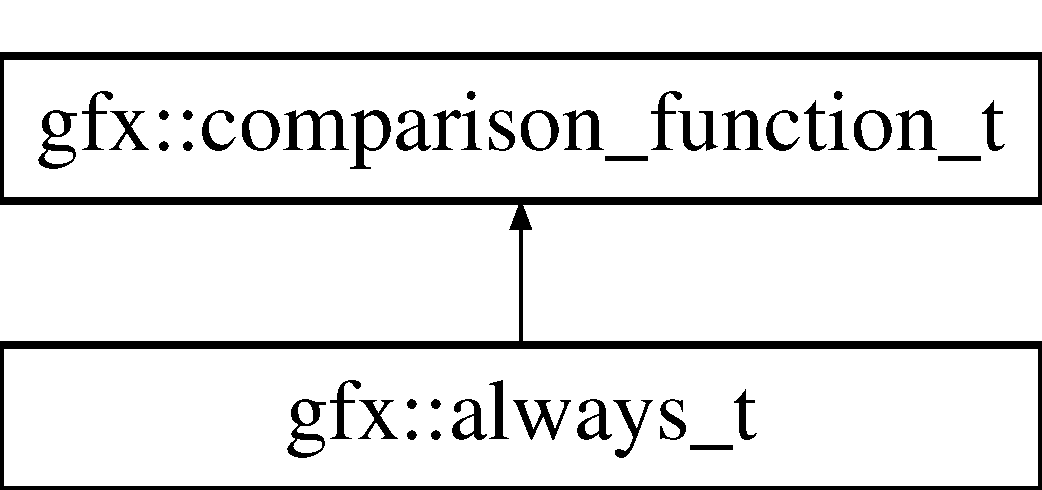
\includegraphics[height=2.000000cm]{classgfx_1_1always__t}
\end{center}
\end{figure}
\subsection*{Protected Member Functions}
\begin{DoxyCompactItemize}
\item 
\hypertarget{classgfx_1_1always__t_a9946abfae3f332483680676d6a5379bf}{virtual G\-Lint {\bfseries val} () const }\label{classgfx_1_1always__t_a9946abfae3f332483680676d6a5379bf}

\end{DoxyCompactItemize}
\subsection*{Friends}
\begin{DoxyCompactItemize}
\item 
\hypertarget{classgfx_1_1always__t_a2039d67f6166ccf823c78e3476aad9aa}{class {\bfseries texture\-\_\-1\-D}}\label{classgfx_1_1always__t_a2039d67f6166ccf823c78e3476aad9aa}

\item 
\hypertarget{classgfx_1_1always__t_a22ad86ef46c3b17357a0cd59e50bc7dd}{class {\bfseries texture\-\_\-2\-D}}\label{classgfx_1_1always__t_a22ad86ef46c3b17357a0cd59e50bc7dd}

\end{DoxyCompactItemize}


\subsection{Detailed Description}
Selector for the always comparison function. 

The documentation for this class was generated from the following file\-:\begin{DoxyCompactItemize}
\item 
g\-Scene/texture.\-hpp\end{DoxyCompactItemize}

\hypertarget{classgfx_1_1binding__error}{\section{gfx\-:\-:binding\-\_\-error Class Reference}
\label{classgfx_1_1binding__error}\index{gfx\-::binding\-\_\-error@{gfx\-::binding\-\_\-error}}
}
Inheritance diagram for gfx\-:\-:binding\-\_\-error\-:\begin{figure}[H]
\begin{center}
\leavevmode
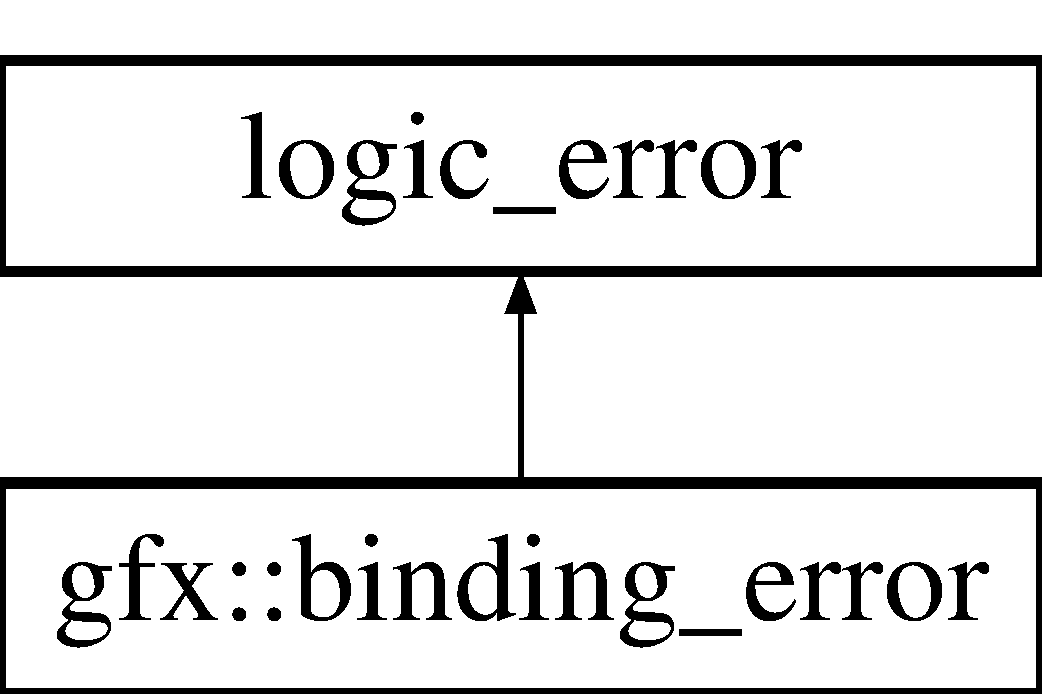
\includegraphics[height=2.000000cm]{classgfx_1_1binding__error}
\end{center}
\end{figure}
\subsection*{Public Member Functions}
\begin{DoxyCompactItemize}
\item 
\hypertarget{classgfx_1_1binding__error_ad5a740fd9d9e9b9ab1bf30645476b89f}{{\bfseries binding\-\_\-error} (std\-::string const \&msg)}\label{classgfx_1_1binding__error_ad5a740fd9d9e9b9ab1bf30645476b89f}

\end{DoxyCompactItemize}


The documentation for this class was generated from the following file\-:\begin{DoxyCompactItemize}
\item 
g\-Video/gfx\-\_\-exception.\-hpp\end{DoxyCompactItemize}

\hypertarget{classgfx_1_1bit__t}{\section{gfx\-:\-:bit\-\_\-t Class Reference}
\label{classgfx_1_1bit__t}\index{gfx\-::bit\-\_\-t@{gfx\-::bit\-\_\-t}}
}


The base class for channel format selectors.  




{\ttfamily \#include \char`\"{}g\-Core/g\-Scene/texture.\-hpp\char`\"{}}

Inheritance diagram for gfx\-:\-:bit\-\_\-t\-:\begin{figure}[H]
\begin{center}
\leavevmode
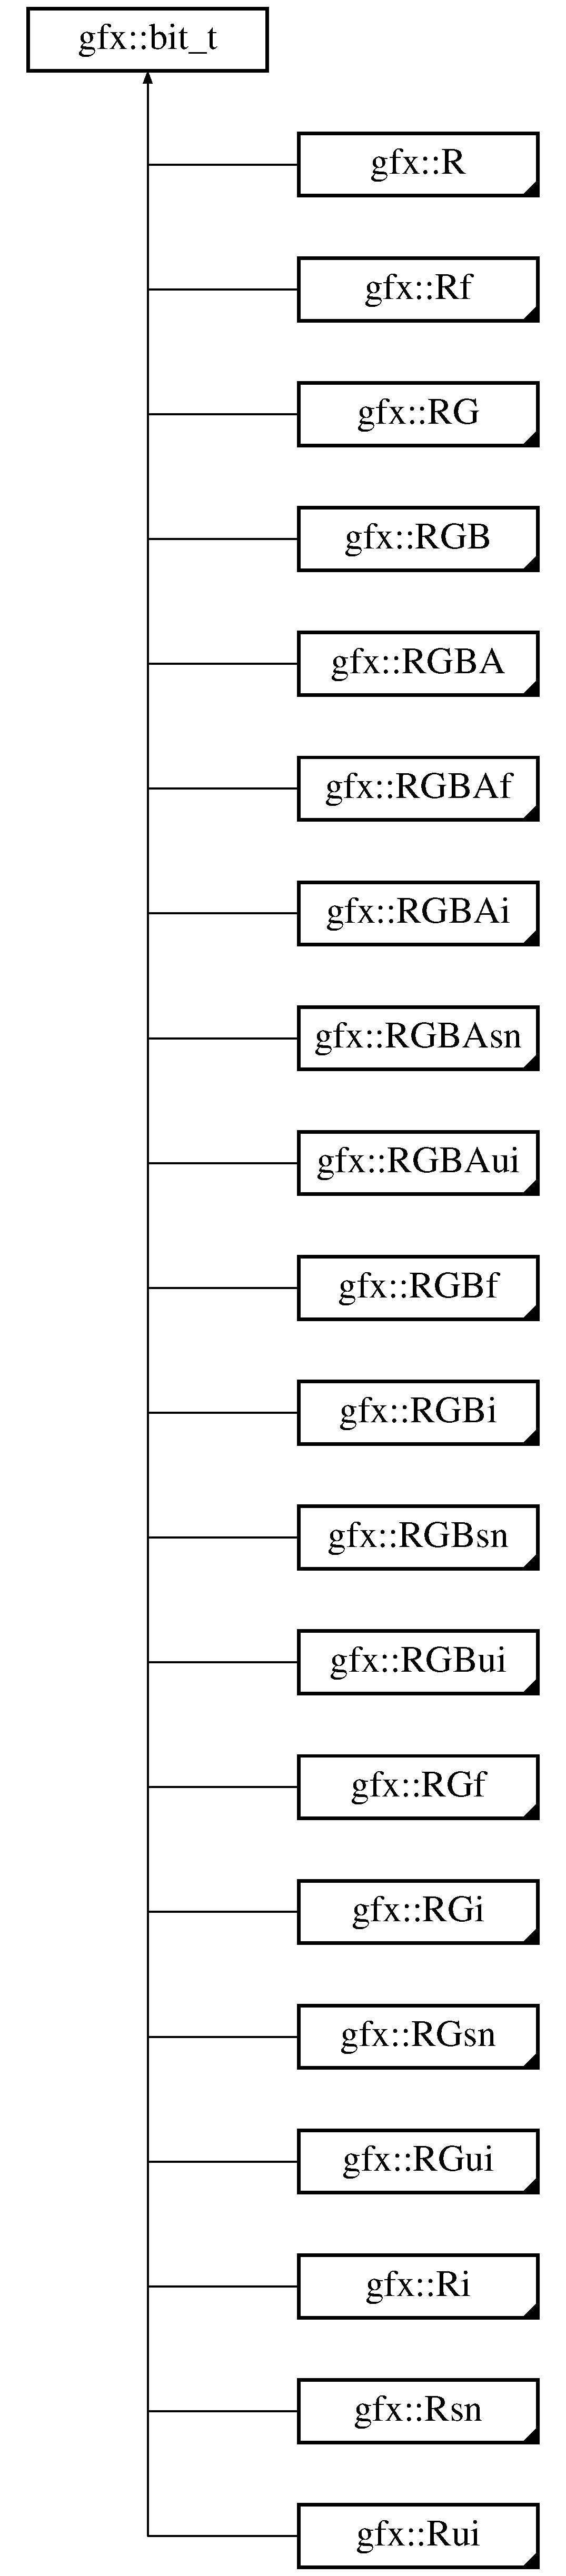
\includegraphics[height=12.000000cm]{classgfx_1_1bit__t}
\end{center}
\end{figure}
\subsection*{Public Member Functions}
\begin{DoxyCompactItemize}
\item 
\hypertarget{classgfx_1_1bit__t_a8d332ea709667a8f386f68391cdb0e44}{virtual size\-\_\-t {\bfseries n} () const =0}\label{classgfx_1_1bit__t_a8d332ea709667a8f386f68391cdb0e44}

\end{DoxyCompactItemize}


\subsection{Detailed Description}
The base class for channel format selectors. 

Channel format selectors are a utility class used in the configuration of textures. Functionally, there are an enum with special type charactersitics to make formatting errors cause compilation errors.

They consist of a multiply inheritted class hierarchy; the derived classes at the end of the hierarchy inherit from the directly derived classes of \hyperlink{classgfx_1_1bit__t}{bit\-\_\-t}. The instances of these terminal classes which are provided are used to select the bit depth of the chanels in the texture, being passed to the number format and chanel multplicity selectors in the settings class.

Using multiple inheritance here means that only combinations of channel bit depth, number format, and chanel mulplicity which are legal in Open\-G\-L are allowed. Illegal combinations cause compilation errors, stopping a developer from making a mistake and causing error messages that more or less actually mean what they say. 

The documentation for this class was generated from the following file\-:\begin{DoxyCompactItemize}
\item 
g\-Scene/texture.\-hpp\end{DoxyCompactItemize}

\hypertarget{classgfx_1_1block__spec}{\section{gfx\-:\-:block\-\_\-spec Class Reference}
\label{classgfx_1_1block__spec}\index{gfx\-::block\-\_\-spec@{gfx\-::block\-\_\-spec}}
}


Describes an ordered block of memory.  




{\ttfamily \#include \char`\"{}g\-Core/g\-Scene/buffer.\-hpp\char`\"{}}

\subsection*{Public Member Functions}
\begin{DoxyCompactItemize}
\item 
\hypertarget{classgfx_1_1block__spec_ab0a36e50fd3ff5c900d565f32073e888}{\hyperlink{classgfx_1_1block__spec_ab0a36e50fd3ff5c900d565f32073e888}{block\-\_\-spec} ()}\label{classgfx_1_1block__spec_ab0a36e50fd3ff5c900d565f32073e888}

\begin{DoxyCompactList}\small\item\em Construct a new, blank, block specification. \end{DoxyCompactList}\item 
\hypertarget{classgfx_1_1block__spec_a573e9b5548ef77f7e2e3a13e266a954d}{\hyperlink{classgfx_1_1block__spec_a573e9b5548ef77f7e2e3a13e266a954d}{$\sim$block\-\_\-spec} ()}\label{classgfx_1_1block__spec_a573e9b5548ef77f7e2e3a13e266a954d}

\begin{DoxyCompactList}\small\item\em Destruct the block specificaiton object. \end{DoxyCompactList}\item 
{\footnotesize template$<$typename T $>$ }\\\hyperlink{classgfx_1_1block__spec}{block\-\_\-spec} \& \hyperlink{classgfx_1_1block__spec_af1330f4cafde86f25c21619f1b472cc3}{attribute} (type$<$ T $>$ const \&proto)
\begin{DoxyCompactList}\small\item\em Add an attribute to the block specification. \end{DoxyCompactList}\item 
\hypertarget{classgfx_1_1block__spec_a57e30d9a1ea24fb2e0bbee663fce839c}{{\footnotesize template$<$typename T $>$ }\\\hyperlink{classgfx_1_1block__spec}{block\-\_\-spec} \& {\bfseries attribute} (type$<$ T $>$ const \&proto)}\label{classgfx_1_1block__spec_a57e30d9a1ea24fb2e0bbee663fce839c}

\end{DoxyCompactItemize}
\subsection*{Friends}
\begin{DoxyCompactItemize}
\item 
\hypertarget{classgfx_1_1block__spec_a38acb51b2a63fccbafac9c0afca0c1b9}{class {\bfseries buffer}}\label{classgfx_1_1block__spec_a38acb51b2a63fccbafac9c0afca0c1b9}

\end{DoxyCompactItemize}


\subsection{Detailed Description}
Describes an ordered block of memory. 

Block specifications are how the formatting of a buffer is defined. The use pattern is the same as the setting objects used for object configuration, except here a templated function is used and the class type is used to encode type information. \begin{DoxySeeAlso}{See Also}
gfx\-::info, gfx\-::type 
\end{DoxySeeAlso}


\subsection{Member Function Documentation}
\hypertarget{classgfx_1_1block__spec_af1330f4cafde86f25c21619f1b472cc3}{\index{gfx\-::block\-\_\-spec@{gfx\-::block\-\_\-spec}!attribute@{attribute}}
\index{attribute@{attribute}!gfx::block_spec@{gfx\-::block\-\_\-spec}}
\subsubsection[{attribute}]{\setlength{\rightskip}{0pt plus 5cm}template$<$typename T $>$ {\bf block\-\_\-spec} \& gfx\-::block\-\_\-spec\-::attribute (
\begin{DoxyParamCaption}
\item[{type$<$ T $>$ const \&}]{proto}
\end{DoxyParamCaption}
)\hspace{0.3cm}{\ttfamily [inline]}}}\label{classgfx_1_1block__spec_af1330f4cafde86f25c21619f1b472cc3}


Add an attribute to the block specification. 

Attributes are added in the order they appear. 

The documentation for this class was generated from the following files\-:\begin{DoxyCompactItemize}
\item 
g\-Scene/block\-\_\-spec.\-hpp\item 
g\-Scene/buffer.\-hpp\item 
g\-Scene/block\-\_\-spec.\-cpp\item 
g\-Scene/buffer.\-cpp\end{DoxyCompactItemize}

\hypertarget{classgfx_1_1box}{\section{gfx\-:\-:box Class Reference}
\label{classgfx_1_1box}\index{gfx\-::box@{gfx\-::box}}
}


A six sided volume with all sides perpendicular to adjacent sides.  




{\ttfamily \#include \char`\"{}g\-Core/g\-Scene/primitive.\-hpp\char`\"{}}

Inheritance diagram for gfx\-:\-:box\-:\begin{figure}[H]
\begin{center}
\leavevmode
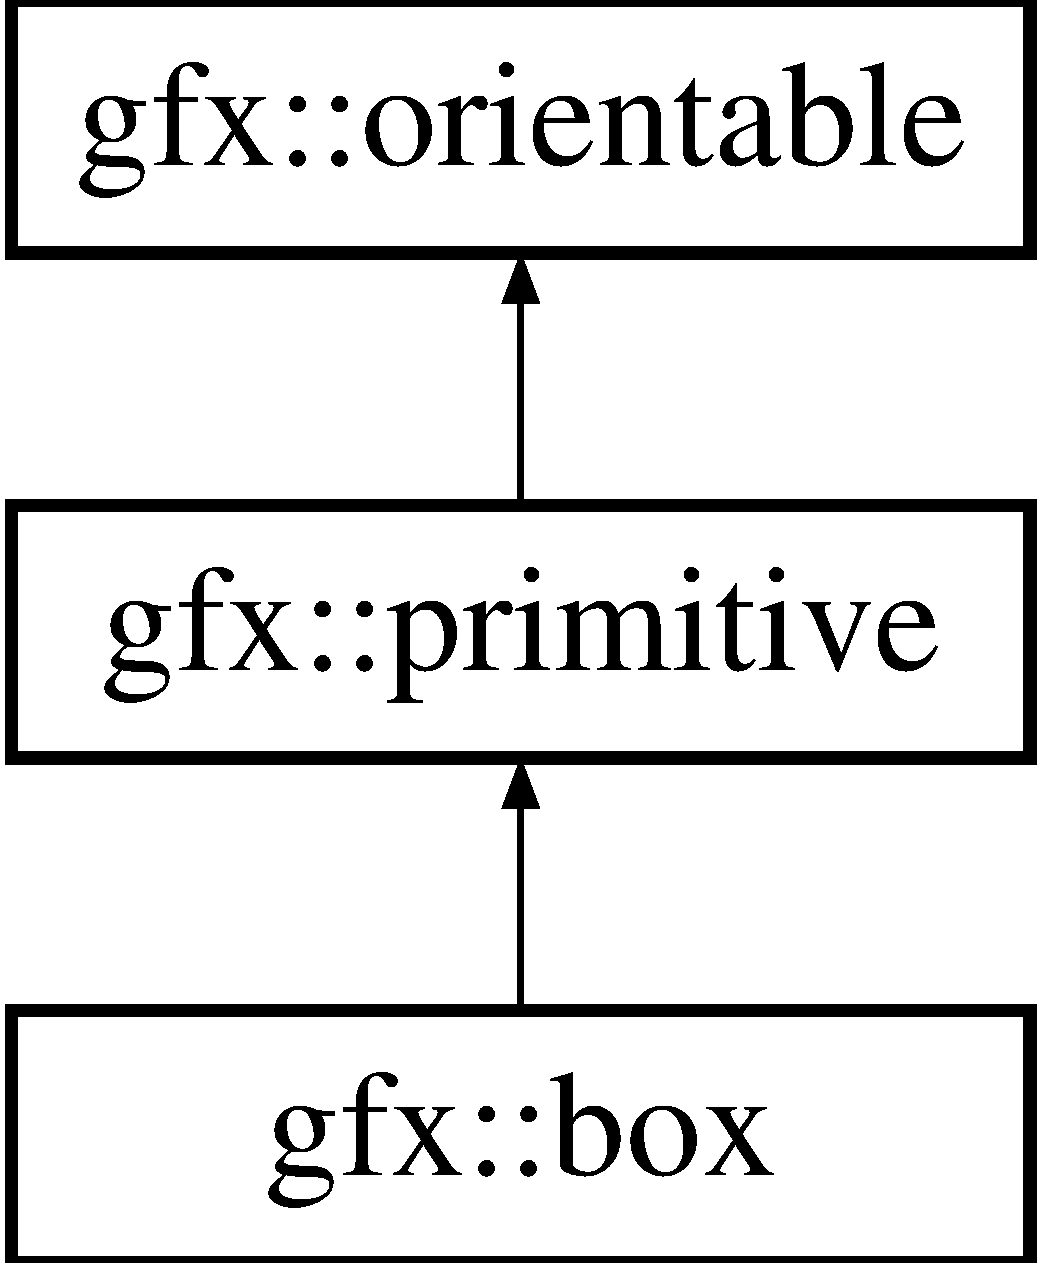
\includegraphics[height=3.000000cm]{classgfx_1_1box}
\end{center}
\end{figure}
\subsection*{Classes}
\begin{DoxyCompactItemize}
\item 
class \hyperlink{classgfx_1_1box_1_1settings}{settings}
\end{DoxyCompactItemize}
\subsection*{Public Member Functions}
\begin{DoxyCompactItemize}
\item 
\hyperlink{classgfx_1_1box_a29298bf9e3c0c7b69ab214a54cc753e3}{box} (\hyperlink{classgfx_1_1box_1_1settings}{settings} const \&set=\hyperlink{classgfx_1_1box_1_1settings}{settings}())
\begin{DoxyCompactList}\small\item\em Construct a new box. \end{DoxyCompactList}\item 
\hyperlink{classgfx_1_1box_a4b955c9dc2402f6d4bb9e59cf34acac4}{$\sim$box} ()
\item 
virtual \hyperlink{classgfx_1_1buffer}{buffer} const \& \hyperlink{classgfx_1_1box_a76d6f6bb065c811cba58d360de6db476}{geometry} () const 
\begin{DoxyCompactList}\small\item\em Return the buffer of the box. \end{DoxyCompactList}\item 
\hypertarget{classgfx_1_1box_ac9d152c560bc2474259266579f251f2e}{G\-Luint $\ast$ \hyperlink{classgfx_1_1box_ac9d152c560bc2474259266579f251f2e}{draw\-\_\-array} ()}\label{classgfx_1_1box_ac9d152c560bc2474259266579f251f2e}

\begin{DoxyCompactList}\small\item\em A\-H\-H\-H\-H\-H\-H\-H\-H\-H\-H\-H\-H\-H\-H\-H\-H\-H\-H\-H\-H!!!!!!!!!!!!!!!!!!! The is just a H\-A\-C\-K. See comments for \hyperlink{classgfx_1_1box_a76d6f6bb065c811cba58d360de6db476}{gfx\-::box\-::geometry} \hyperlink{classgfx_1_1box_a76d6f6bb065c811cba58d360de6db476}{geometry()}. \end{DoxyCompactList}\end{DoxyCompactItemize}
\subsection*{Additional Inherited Members}


\subsection{Detailed Description}
A six sided volume with all sides perpendicular to adjacent sides. 

\subsection{Constructor \& Destructor Documentation}
\hypertarget{classgfx_1_1box_a29298bf9e3c0c7b69ab214a54cc753e3}{\index{gfx\-::box@{gfx\-::box}!box@{box}}
\index{box@{box}!gfx::box@{gfx\-::box}}
\subsubsection[{box}]{\setlength{\rightskip}{0pt plus 5cm}gfx\-::box\-::box (
\begin{DoxyParamCaption}
\item[{{\bf box\-::settings} const \&}]{set = {\ttfamily {\bf settings}()}}
\end{DoxyParamCaption}
)}}\label{classgfx_1_1box_a29298bf9e3c0c7b69ab214a54cc753e3}


Construct a new box. 


\begin{DoxyParams}{Parameters}
{\em set} & The settings object ofr this box. \\
\hline
\end{DoxyParams}
\hypertarget{classgfx_1_1box_a4b955c9dc2402f6d4bb9e59cf34acac4}{\index{gfx\-::box@{gfx\-::box}!$\sim$box@{$\sim$box}}
\index{$\sim$box@{$\sim$box}!gfx::box@{gfx\-::box}}
\subsubsection[{$\sim$box}]{\setlength{\rightskip}{0pt plus 5cm}gfx\-::box\-::$\sim$box (
\begin{DoxyParamCaption}
{}
\end{DoxyParamCaption}
)}}\label{classgfx_1_1box_a4b955c9dc2402f6d4bb9e59cf34acac4}
Destruct this box. 

\subsection{Member Function Documentation}
\hypertarget{classgfx_1_1box_a76d6f6bb065c811cba58d360de6db476}{\index{gfx\-::box@{gfx\-::box}!geometry@{geometry}}
\index{geometry@{geometry}!gfx::box@{gfx\-::box}}
\subsubsection[{geometry}]{\setlength{\rightskip}{0pt plus 5cm}{\bf buffer} const \& gfx\-::box\-::geometry (
\begin{DoxyParamCaption}
{}
\end{DoxyParamCaption}
) const\hspace{0.3cm}{\ttfamily [inline]}, {\ttfamily [virtual]}}}\label{classgfx_1_1box_a76d6f6bb065c811cba58d360de6db476}


Return the buffer of the box. 

Using the buffer you can draw the box with Open\-G\-L. I do not like this method of drawing primtives, or any geometry for that matter. The ideal solution is a 'technique' class that synthesizes the drawing settings and tools like programs paired with a 'drawable' interface to define how geometry is provided. 

Implements \hyperlink{classgfx_1_1primitive}{gfx\-::primitive}.



The documentation for this class was generated from the following files\-:\begin{DoxyCompactItemize}
\item 
g\-Scene/primitive.\-hpp\item 
g\-Scene/primitive.\-cpp\end{DoxyCompactItemize}

\hypertarget{classgfx_1_1buffer}{\section{gfx\-:\-:buffer Class Reference}
\label{classgfx_1_1buffer}\index{gfx\-::buffer@{gfx\-::buffer}}
}


A base class that provides the interface to deal with Open\-G\-L buffers.  




{\ttfamily \#include \char`\"{}g\-Core/g\-Scene/buffer.\-hpp\char`\"{}}

Inheritance diagram for gfx\-:\-:buffer\-:\begin{figure}[H]
\begin{center}
\leavevmode
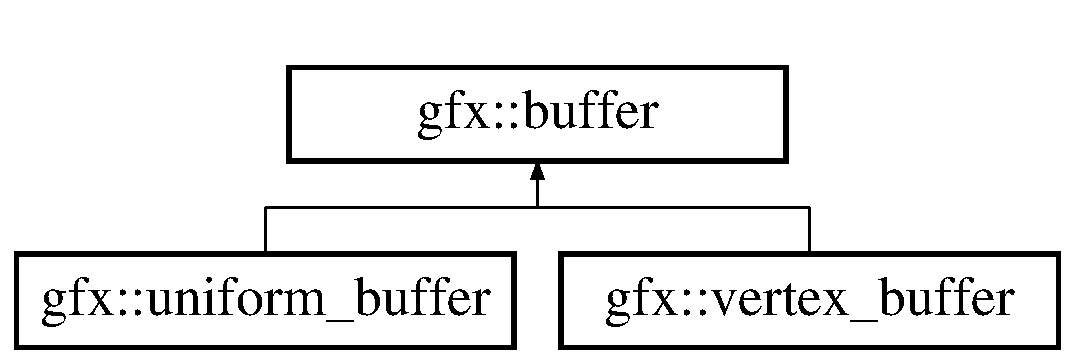
\includegraphics[height=2.000000cm]{classgfx_1_1buffer}
\end{center}
\end{figure}
\subsection*{Classes}
\begin{DoxyCompactItemize}
\item 
class \hyperlink{classgfx_1_1buffer_1_1settings}{settings}
\end{DoxyCompactItemize}
\subsection*{Public Member Functions}
\begin{DoxyCompactItemize}
\item 
\hyperlink{classgfx_1_1buffer_a78a4247848a19c74a77410c92f0455d3}{buffer} (\hyperlink{classgfx_1_1buffer_1_1settings}{settings} const \&set=\hyperlink{classgfx_1_1buffer_1_1settings}{settings}())
\begin{DoxyCompactList}\small\item\em Construct a new \hyperlink{classgfx_1_1buffer}{buffer} object. \end{DoxyCompactList}\item 
\hypertarget{classgfx_1_1buffer_a2b267c96867b14486ee9200b758a3246}{virtual \hyperlink{classgfx_1_1buffer_a2b267c96867b14486ee9200b758a3246}{$\sim$buffer} ()}\label{classgfx_1_1buffer_a2b267c96867b14486ee9200b758a3246}

\begin{DoxyCompactList}\small\item\em Destruct the buffer. \end{DoxyCompactList}\item 
void \hyperlink{classgfx_1_1buffer_ad9b89548222f37163c44f402e8577110}{block\-\_\-format} (\hyperlink{classgfx_1_1block__spec}{block\-\_\-spec} const \&spec)
\begin{DoxyCompactList}\small\item\em Use the given block specification to format the data of the buffer. \end{DoxyCompactList}\item 
G\-Lsizeiptr \hyperlink{classgfx_1_1buffer_a21c20dcd317940802016dc93f1e38f19}{size} () const 
\begin{DoxyCompactList}\small\item\em Query the \hyperlink{classgfx_1_1buffer}{buffer} for its size. \end{DoxyCompactList}\item 
void \hyperlink{classgfx_1_1buffer_a9c4e3ba0b7794299c80cd400bd6625f8}{blocks} (G\-Lsizeiptr const blocks)
\begin{DoxyCompactList}\small\item\em Set the number of data blocks in the \hyperlink{classgfx_1_1buffer}{buffer}. \end{DoxyCompactList}\item 
void \hyperlink{classgfx_1_1buffer_a08cffdcb5184e6ff8fec0df1ad817163}{add\-\_\-blocks} (G\-Lsizeiptr const more\-\_\-blocks)
\begin{DoxyCompactList}\small\item\em Expand the number of data blocks in the \hyperlink{classgfx_1_1buffer}{buffer}. \end{DoxyCompactList}\item 
{\footnotesize template$<$typename D\-A\-T\-A $>$ }\\void \hyperlink{classgfx_1_1buffer_a44af69c977b694cce9b5014f6440efc9}{load\-\_\-attribute} (G\-Luint index, std\-::vector$<$ D\-A\-T\-A $>$ const \&attrib\-\_\-data)
\begin{DoxyCompactList}\small\item\em Load data into the \hyperlink{classgfx_1_1buffer}{buffer}. \end{DoxyCompactList}\item 
virtual void \hyperlink{classgfx_1_1buffer_a7019485ae327de1d5d5525185196ff43}{upload\-\_\-data} ()
\begin{DoxyCompactList}\small\item\em Upload the \hyperlink{classgfx_1_1buffer}{buffer's} data to Open\-G\-L. \end{DoxyCompactList}\item 
\hypertarget{classgfx_1_1buffer_a8395dfeccf42d150dd698211d361fcec}{virtual void {\bfseries align} ()=0}\label{classgfx_1_1buffer_a8395dfeccf42d150dd698211d361fcec}

\end{DoxyCompactItemize}
\subsection*{Protected Types}
\begin{DoxyCompactItemize}
\item 
\hypertarget{classgfx_1_1buffer_a85c93d8e695b4715401764267e27b23c}{typedef std\-::vector$<$ info $\ast$ $>$ {\bfseries attrib\-\_\-vector}}\label{classgfx_1_1buffer_a85c93d8e695b4715401764267e27b23c}

\end{DoxyCompactItemize}
\subsection*{Protected Member Functions}
\begin{DoxyCompactItemize}
\item 
G\-Lsizeiptr \hyperlink{classgfx_1_1buffer_afafe95bbac44b4392e48f04cbffb16a9}{attribute\-\_\-offset} (G\-Luint index) const 
\begin{DoxyCompactList}\small\item\em Query the \hyperlink{classgfx_1_1buffer}{buffer} for the byte offset of the attribute with the given index. \end{DoxyCompactList}\end{DoxyCompactItemize}
\subsection*{Protected Attributes}
\begin{DoxyCompactItemize}
\item 
\hypertarget{classgfx_1_1buffer_ab5b0ca79b5c3058d3cfa707f029f9119}{unsigned char $\ast$ {\bfseries data}}\label{classgfx_1_1buffer_ab5b0ca79b5c3058d3cfa707f029f9119}

\item 
\hypertarget{classgfx_1_1buffer_abeb05ba5f2a55cd25f88ad70bd05a8b8}{G\-Lsizeiptr {\bfseries n\-\_\-blocks}}\label{classgfx_1_1buffer_abeb05ba5f2a55cd25f88ad70bd05a8b8}

\item 
\hypertarget{classgfx_1_1buffer_a5bb5ae77f00821dde719f2ec03b5d0e6}{G\-Lsizeiptr {\bfseries stride}}\label{classgfx_1_1buffer_a5bb5ae77f00821dde719f2ec03b5d0e6}

\item 
\hypertarget{classgfx_1_1buffer_accc9828ba943b976549f07ae06e05e35}{G\-Luint {\bfseries buff\-\_\-\-I\-D}}\label{classgfx_1_1buffer_accc9828ba943b976549f07ae06e05e35}

\item 
\hypertarget{classgfx_1_1buffer_ab00ffc79a1d96212511f90569a4e7bcc}{G\-Lenum {\bfseries usage}}\label{classgfx_1_1buffer_ab00ffc79a1d96212511f90569a4e7bcc}

\item 
\hypertarget{classgfx_1_1buffer_a891c9e8489ada44e36520a79edd6e1fa}{G\-Lenum {\bfseries intended\-\_\-target}}\label{classgfx_1_1buffer_a891c9e8489ada44e36520a79edd6e1fa}

\item 
\hypertarget{classgfx_1_1buffer_a2364b41ea3e767a2605002964d043e0c}{bool {\bfseries data\-\_\-loaded}}\label{classgfx_1_1buffer_a2364b41ea3e767a2605002964d043e0c}

\item 
\hypertarget{classgfx_1_1buffer_acd441d5dda07ce4b5f48c797fc50f060}{bool {\bfseries verts\-\_\-specified}}\label{classgfx_1_1buffer_acd441d5dda07ce4b5f48c797fc50f060}

\item 
\hypertarget{classgfx_1_1buffer_a42f2bd5d967e8aad51333e76862a3547}{attrib\-\_\-vector $\ast$ {\bfseries attributes}}\label{classgfx_1_1buffer_a42f2bd5d967e8aad51333e76862a3547}

\end{DoxyCompactItemize}
\subsection*{Friends}
\begin{DoxyCompactItemize}
\item 
\hypertarget{classgfx_1_1buffer_aae00f29dd994b9fe4e742376ae3073bf}{std\-::ostream \& {\bfseries operator$<$$<$} (std\-::ostream \&out, \hyperlink{classgfx_1_1buffer}{buffer} const \&rhs)}\label{classgfx_1_1buffer_aae00f29dd994b9fe4e742376ae3073bf}

\end{DoxyCompactItemize}


\subsection{Detailed Description}
A base class that provides the interface to deal with Open\-G\-L buffers. 

All the common functionality of the different uses for Open\-G\-L buffers is included in the buffer class. The specific use cases are implemented in derived classes, which in some cases may override certain settings that must have particular values for that use case. \begin{DoxyRefDesc}{Todo}
\item[\hyperlink{todo__todo000013}{Todo}]Review those settings that may get overriden; perhaps they chould be removed as user-\/settable settings because the presence of pure virtual functions in this class means it can never be instantiated and so the idea that you could hack your own use of this class is a dead end. If it is removed, perhaps it would be useful to move the settings mutators into a protected interface for derived classes.\end{DoxyRefDesc}


\begin{DoxyRefDesc}{Todo}
\item[\hyperlink{todo__todo000014}{Todo}]Also, maybe reduce the settings interface and separate the static-\/dynamic-\/stream from the draw-\/read-\/copy. \end{DoxyRefDesc}


\subsection{Constructor \& Destructor Documentation}
\hypertarget{classgfx_1_1buffer_a78a4247848a19c74a77410c92f0455d3}{\index{gfx\-::buffer@{gfx\-::buffer}!buffer@{buffer}}
\index{buffer@{buffer}!gfx::buffer@{gfx\-::buffer}}
\subsubsection[{buffer}]{\setlength{\rightskip}{0pt plus 5cm}gfx\-::buffer\-::buffer (
\begin{DoxyParamCaption}
\item[{{\bf settings} const \&}]{set = {\ttfamily {\bf settings}()}}
\end{DoxyParamCaption}
)}}\label{classgfx_1_1buffer_a78a4247848a19c74a77410c92f0455d3}


Construct a new \hyperlink{classgfx_1_1buffer}{buffer} object. 


\begin{DoxyParams}{Parameters}
{\em set} & The settings for the new buffer object. \\
\hline
\end{DoxyParams}


\subsection{Member Function Documentation}
\hypertarget{classgfx_1_1buffer_a08cffdcb5184e6ff8fec0df1ad817163}{\index{gfx\-::buffer@{gfx\-::buffer}!add\-\_\-blocks@{add\-\_\-blocks}}
\index{add\-\_\-blocks@{add\-\_\-blocks}!gfx::buffer@{gfx\-::buffer}}
\subsubsection[{add\-\_\-blocks}]{\setlength{\rightskip}{0pt plus 5cm}void gfx\-::buffer\-::add\-\_\-blocks (
\begin{DoxyParamCaption}
\item[{G\-Lsizeiptr const}]{more\-\_\-blocks}
\end{DoxyParamCaption}
)}}\label{classgfx_1_1buffer_a08cffdcb5184e6ff8fec0df1ad817163}


Expand the number of data blocks in the \hyperlink{classgfx_1_1buffer}{buffer}. 

This will reallocate the internal memory in order to resize it, copying whatever data has been uploaded via \hyperlink{classgfx_1_1buffer_a44af69c977b694cce9b5014f6440efc9}{load\-\_\-attribute()} into the new memory, as far as it can fit. \begin{DoxyRefDesc}{Todo}
\item[\hyperlink{todo__todo000010}{Todo}]The copying functionality, as implemented, is wrong. Either fix the loop or remove the copying. 
\begin{DoxyParams}{Parameters}
{\em more\-\_\-blocks} & The number of blocks to add to the buffer \\
\hline
\end{DoxyParams}
\end{DoxyRefDesc}
\hypertarget{classgfx_1_1buffer_afafe95bbac44b4392e48f04cbffb16a9}{\index{gfx\-::buffer@{gfx\-::buffer}!attribute\-\_\-offset@{attribute\-\_\-offset}}
\index{attribute\-\_\-offset@{attribute\-\_\-offset}!gfx::buffer@{gfx\-::buffer}}
\subsubsection[{attribute\-\_\-offset}]{\setlength{\rightskip}{0pt plus 5cm}G\-Lsizeiptr gfx\-::buffer\-::attribute\-\_\-offset (
\begin{DoxyParamCaption}
\item[{G\-Luint}]{index}
\end{DoxyParamCaption}
) const\hspace{0.3cm}{\ttfamily [protected]}}}\label{classgfx_1_1buffer_afafe95bbac44b4392e48f04cbffb16a9}


Query the \hyperlink{classgfx_1_1buffer}{buffer} for the byte offset of the attribute with the given index. 

This is probably not going to stick around; it exposes the internals of Open\-G\-L and the buffer class too much. More of a thing to hack functionality that isn't implemented yet, and to be honest I don't know if it even used. \begin{DoxyRefDesc}{Todo}
\item[\hyperlink{todo__todo000012}{Todo}]Review for deprecation or removal 
\begin{DoxyParams}{Parameters}
{\em index} & The index of the attribute to get the offset of \\
\hline
\end{DoxyParams}
\end{DoxyRefDesc}
\hypertarget{classgfx_1_1buffer_ad9b89548222f37163c44f402e8577110}{\index{gfx\-::buffer@{gfx\-::buffer}!block\-\_\-format@{block\-\_\-format}}
\index{block\-\_\-format@{block\-\_\-format}!gfx::buffer@{gfx\-::buffer}}
\subsubsection[{block\-\_\-format}]{\setlength{\rightskip}{0pt plus 5cm}void gfx\-::buffer\-::block\-\_\-format (
\begin{DoxyParamCaption}
\item[{{\bf block\-\_\-spec} const \&}]{spec}
\end{DoxyParamCaption}
)}}\label{classgfx_1_1buffer_ad9b89548222f37163c44f402e8577110}


Use the given block specification to format the data of the buffer. 

Each time you call this function, the format is completely overwritten. 
\begin{DoxyParams}{Parameters}
{\em spec} & The block specification describing the formatting of the buffer. \\
\hline
\end{DoxyParams}
\hypertarget{classgfx_1_1buffer_a9c4e3ba0b7794299c80cd400bd6625f8}{\index{gfx\-::buffer@{gfx\-::buffer}!blocks@{blocks}}
\index{blocks@{blocks}!gfx::buffer@{gfx\-::buffer}}
\subsubsection[{blocks}]{\setlength{\rightskip}{0pt plus 5cm}void gfx\-::buffer\-::blocks (
\begin{DoxyParamCaption}
\item[{G\-Lsizeiptr const}]{blocks}
\end{DoxyParamCaption}
)}}\label{classgfx_1_1buffer_a9c4e3ba0b7794299c80cd400bd6625f8}


Set the number of data blocks in the \hyperlink{classgfx_1_1buffer}{buffer}. 

This will reallocate the internal memory in order to resize it, copying whatever data has been uploaded via \hyperlink{classgfx_1_1buffer_a44af69c977b694cce9b5014f6440efc9}{load\-\_\-attribute()} into the new memory, as far as it can fit. \begin{DoxyRefDesc}{Todo}
\item[\hyperlink{todo__todo000009}{Todo}]The copying functionality, as implemented, is wrong. Either fix the loop or remove the copying. 
\begin{DoxyParams}{Parameters}
{\em blocks} & The number of blocks the buffer now has \\
\hline
\end{DoxyParams}
\end{DoxyRefDesc}
\hypertarget{classgfx_1_1buffer_a44af69c977b694cce9b5014f6440efc9}{\index{gfx\-::buffer@{gfx\-::buffer}!load\-\_\-attribute@{load\-\_\-attribute}}
\index{load\-\_\-attribute@{load\-\_\-attribute}!gfx::buffer@{gfx\-::buffer}}
\subsubsection[{load\-\_\-attribute}]{\setlength{\rightskip}{0pt plus 5cm}template$<$typename D\-A\-T\-A $>$ void gfx\-::buffer\-::load\-\_\-attribute (
\begin{DoxyParamCaption}
\item[{G\-Luint}]{index, }
\item[{std\-::vector$<$ D\-A\-T\-A $>$ const \&}]{attrib\-\_\-data}
\end{DoxyParamCaption}
)}}\label{classgfx_1_1buffer_a44af69c977b694cce9b5014f6440efc9}


Load data into the \hyperlink{classgfx_1_1buffer}{buffer}. 


\begin{DoxyParams}{Parameters}
{\em attrib\-\_\-data} & The source data for the buffer \\
\hline
\end{DoxyParams}
\hypertarget{classgfx_1_1buffer_a21c20dcd317940802016dc93f1e38f19}{\index{gfx\-::buffer@{gfx\-::buffer}!size@{size}}
\index{size@{size}!gfx::buffer@{gfx\-::buffer}}
\subsubsection[{size}]{\setlength{\rightskip}{0pt plus 5cm}G\-Lsizeiptr gfx\-::buffer\-::size (
\begin{DoxyParamCaption}
{}
\end{DoxyParamCaption}
) const\hspace{0.3cm}{\ttfamily [inline]}}}\label{classgfx_1_1buffer_a21c20dcd317940802016dc93f1e38f19}


Query the \hyperlink{classgfx_1_1buffer}{buffer} for its size. 

\begin{DoxyReturn}{Returns}
The number of blocks in the buffer 
\end{DoxyReturn}
\hypertarget{classgfx_1_1buffer_a7019485ae327de1d5d5525185196ff43}{\index{gfx\-::buffer@{gfx\-::buffer}!upload\-\_\-data@{upload\-\_\-data}}
\index{upload\-\_\-data@{upload\-\_\-data}!gfx::buffer@{gfx\-::buffer}}
\subsubsection[{upload\-\_\-data}]{\setlength{\rightskip}{0pt plus 5cm}void gfx\-::buffer\-::upload\-\_\-data (
\begin{DoxyParamCaption}
{}
\end{DoxyParamCaption}
)\hspace{0.3cm}{\ttfamily [virtual]}}}\label{classgfx_1_1buffer_a7019485ae327de1d5d5525185196ff43}


Upload the \hyperlink{classgfx_1_1buffer}{buffer's} data to Open\-G\-L. 

\begin{DoxyRefDesc}{Todo}
\item[\hyperlink{todo__todo000011}{Todo}]There is no check to see if you have actually specified the data format. This means, internally, the stride member has not been correctly specified and so the upload will send Open\-G\-L an unpredictable number of bytes (usually 0 but in more complex use cases it could be anything depending on the lifetime of the particular buffer). It also doesn't check to see if you have even loaded any data into the buffer client-\/ side or if the buffer is \char`\"{}dirty\char`\"{}. Though that is not quite as bad, it certainly isn't very helpful for the user. \end{DoxyRefDesc}


Reimplemented in \hyperlink{classgfx_1_1vertex__buffer_a3248a790af715bc3b211d81ffd8a686b}{gfx\-::vertex\-\_\-buffer}.



The documentation for this class was generated from the following files\-:\begin{DoxyCompactItemize}
\item 
g\-Scene/buffer.\-hpp\item 
g\-Scene/buffer.\-cpp\end{DoxyCompactItemize}

\hypertarget{classgfx_1_1camera}{\section{gfx\-:\-:camera Class Reference}
\label{classgfx_1_1camera}\index{gfx\-::camera@{gfx\-::camera}}
}


A base class for cameras.  




{\ttfamily \#include \char`\"{}g\-Core/g\-Scene/camera.\-hpp\char`\"{}}

Inheritance diagram for gfx\-:\-:camera\-:\begin{figure}[H]
\begin{center}
\leavevmode
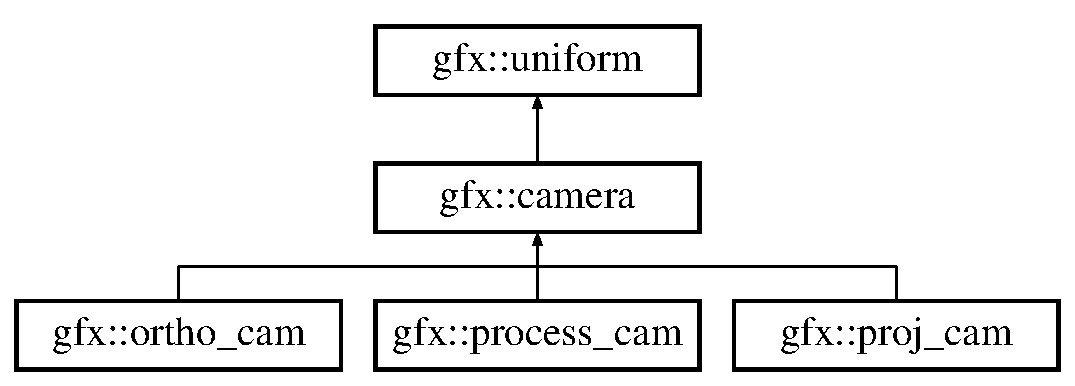
\includegraphics[height=3.000000cm]{classgfx_1_1camera}
\end{center}
\end{figure}
\subsection*{Public Member Functions}
\begin{DoxyCompactItemize}
\item 
\hypertarget{classgfx_1_1camera_a79ba46c37d81a5607e3432eabb75ebd7}{\hyperlink{classgfx_1_1camera_a79ba46c37d81a5607e3432eabb75ebd7}{camera} ()}\label{classgfx_1_1camera_a79ba46c37d81a5607e3432eabb75ebd7}

\begin{DoxyCompactList}\small\item\em Construct a new camera. \end{DoxyCompactList}\item 
\hypertarget{classgfx_1_1camera_a2f2ce94351b2fa823cada43be12ab0c7}{\hyperlink{classgfx_1_1camera_a2f2ce94351b2fa823cada43be12ab0c7}{$\sim$camera} ()}\label{classgfx_1_1camera_a2f2ce94351b2fa823cada43be12ab0c7}

\begin{DoxyCompactList}\small\item\em Destruct this camera. \end{DoxyCompactList}\item 
virtual void \hyperlink{classgfx_1_1camera_a209884984c107ef76442b6408dc4f822}{upload\-\_\-uniform} (\hyperlink{classgfx_1_1program}{program} \&prgm, std\-::string const \&name)
\begin{DoxyCompactList}\small\item\em Upload this camera as a uniform to the program given. \end{DoxyCompactList}\item 
mat4 const \& \hyperlink{classgfx_1_1camera_a6c8a9dabd500a55ba6446836d9323aef}{view\-\_\-matrix} ()
\begin{DoxyCompactList}\small\item\em Return the view matrix of this camera. \end{DoxyCompactList}\end{DoxyCompactItemize}
\subsection*{Protected Member Functions}
\begin{DoxyCompactItemize}
\item 
\hypertarget{classgfx_1_1camera_a155cec0462b4616674299cf6400a2ad9}{virtual void {\bfseries update\-\_\-view} ()=0}\label{classgfx_1_1camera_a155cec0462b4616674299cf6400a2ad9}

\end{DoxyCompactItemize}
\subsection*{Protected Attributes}
\begin{DoxyCompactItemize}
\item 
\hypertarget{classgfx_1_1camera_a735ae8c490ef7f95f6167d7ef849d89b}{bool {\bfseries view\-\_\-changed}}\label{classgfx_1_1camera_a735ae8c490ef7f95f6167d7ef849d89b}

\item 
\hypertarget{classgfx_1_1camera_a9cc17514a4d80b914f7be393d2b5db39}{mat4 {\bfseries view}}\label{classgfx_1_1camera_a9cc17514a4d80b914f7be393d2b5db39}

\end{DoxyCompactItemize}


\subsection{Detailed Description}
A base class for cameras. 

Cameras need only implement the why the view matrix is updated. 

\subsection{Member Function Documentation}
\hypertarget{classgfx_1_1camera_a209884984c107ef76442b6408dc4f822}{\index{gfx\-::camera@{gfx\-::camera}!upload\-\_\-uniform@{upload\-\_\-uniform}}
\index{upload\-\_\-uniform@{upload\-\_\-uniform}!gfx::camera@{gfx\-::camera}}
\subsubsection[{upload\-\_\-uniform}]{\setlength{\rightskip}{0pt plus 5cm}void gfx\-::camera\-::upload\-\_\-uniform (
\begin{DoxyParamCaption}
\item[{{\bf program} \&}]{prgm, }
\item[{std\-::string const \&}]{name}
\end{DoxyParamCaption}
)\hspace{0.3cm}{\ttfamily [virtual]}}}\label{classgfx_1_1camera_a209884984c107ef76442b6408dc4f822}


Upload this camera as a uniform to the program given. 

At the moment, this function requires that you have first specified the names of the fields in a camera manually in the program object. \begin{DoxyRefDesc}{Todo}
\item[\hyperlink{todo__todo000015}{Todo}]Fix this uniform problem 
\begin{DoxyParams}{Parameters}
{\em prgm} & The program to upload the uniform to \\
\hline
{\em name} & The name of the camera variable in the shader source \\
\hline
\end{DoxyParams}
\end{DoxyRefDesc}


Implements \hyperlink{classgfx_1_1uniform}{gfx\-::uniform}.

\hypertarget{classgfx_1_1camera_a6c8a9dabd500a55ba6446836d9323aef}{\index{gfx\-::camera@{gfx\-::camera}!view\-\_\-matrix@{view\-\_\-matrix}}
\index{view\-\_\-matrix@{view\-\_\-matrix}!gfx::camera@{gfx\-::camera}}
\subsubsection[{view\-\_\-matrix}]{\setlength{\rightskip}{0pt plus 5cm}mat4 const \& gfx\-::camera\-::view\-\_\-matrix (
\begin{DoxyParamCaption}
{}
\end{DoxyParamCaption}
)}}\label{classgfx_1_1camera_a6c8a9dabd500a55ba6446836d9323aef}


Return the view matrix of this camera. 

\begin{DoxyReturn}{Returns}
The view matrix 
\end{DoxyReturn}


The documentation for this class was generated from the following files\-:\begin{DoxyCompactItemize}
\item 
g\-Scene/camera.\-hpp\item 
g\-Scene/camera.\-cpp\end{DoxyCompactItemize}

\hypertarget{classgfx_1_1clamp__to__border__t}{\section{gfx\-:\-:clamp\-\_\-to\-\_\-border\-\_\-t Class Reference}
\label{classgfx_1_1clamp__to__border__t}\index{gfx\-::clamp\-\_\-to\-\_\-border\-\_\-t@{gfx\-::clamp\-\_\-to\-\_\-border\-\_\-t}}
}


Selector for clamp to border sampling.  




{\ttfamily \#include \char`\"{}g\-Core/g\-Video/texture.\-hpp\char`\"{}}

Inheritance diagram for gfx\-:\-:clamp\-\_\-to\-\_\-border\-\_\-t\-:\begin{figure}[H]
\begin{center}
\leavevmode
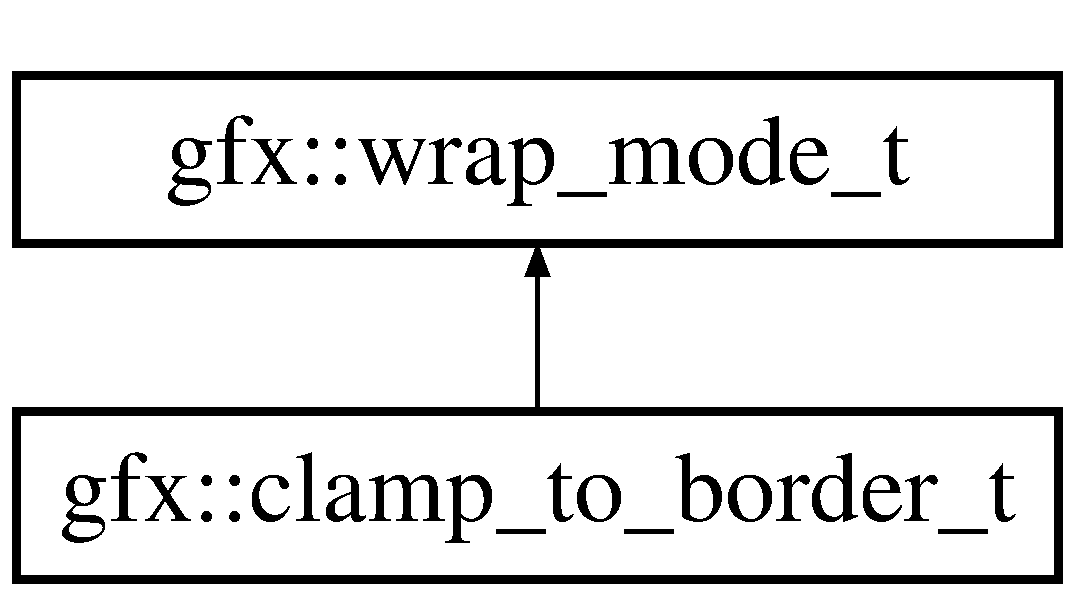
\includegraphics[height=2.000000cm]{classgfx_1_1clamp__to__border__t}
\end{center}
\end{figure}
\subsection*{Protected Member Functions}
\begin{DoxyCompactItemize}
\item 
\hypertarget{classgfx_1_1clamp__to__border__t_a108f12c0c35494ad0407ec46b549ab2c}{virtual G\-Lint {\bfseries val} () const }\label{classgfx_1_1clamp__to__border__t_a108f12c0c35494ad0407ec46b549ab2c}

\end{DoxyCompactItemize}
\subsection*{Friends}
\begin{DoxyCompactItemize}
\item 
\hypertarget{classgfx_1_1clamp__to__border__t_a2039d67f6166ccf823c78e3476aad9aa}{class {\bfseries texture\-\_\-1\-D}}\label{classgfx_1_1clamp__to__border__t_a2039d67f6166ccf823c78e3476aad9aa}

\item 
\hypertarget{classgfx_1_1clamp__to__border__t_a22ad86ef46c3b17357a0cd59e50bc7dd}{class {\bfseries texture\-\_\-2\-D}}\label{classgfx_1_1clamp__to__border__t_a22ad86ef46c3b17357a0cd59e50bc7dd}

\end{DoxyCompactItemize}


\subsection{Detailed Description}
Selector for clamp to border sampling. 

The documentation for this class was generated from the following file\-:\begin{DoxyCompactItemize}
\item 
g\-Scene/texture.\-hpp\end{DoxyCompactItemize}

\hypertarget{classgfx_1_1clamp__to__edge__t}{\section{gfx\-:\-:clamp\-\_\-to\-\_\-edge\-\_\-t Class Reference}
\label{classgfx_1_1clamp__to__edge__t}\index{gfx\-::clamp\-\_\-to\-\_\-edge\-\_\-t@{gfx\-::clamp\-\_\-to\-\_\-edge\-\_\-t}}
}


Selector for clamp to edge sampling.  




{\ttfamily \#include \char`\"{}g\-Core/g\-Video/texture.\-hpp\char`\"{}}

Inheritance diagram for gfx\-:\-:clamp\-\_\-to\-\_\-edge\-\_\-t\-:\begin{figure}[H]
\begin{center}
\leavevmode
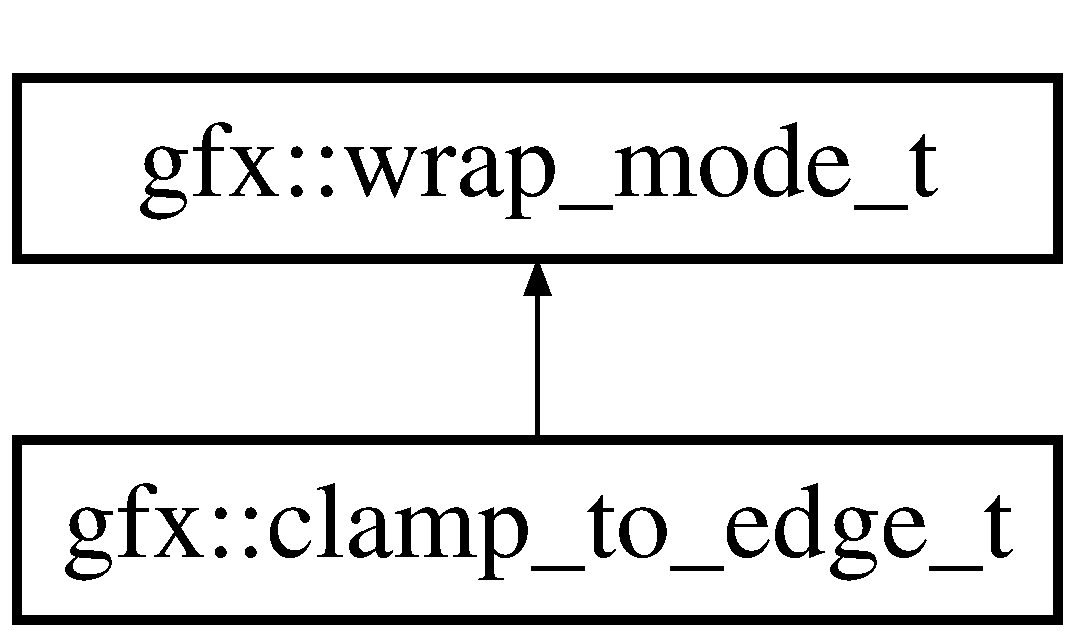
\includegraphics[height=2.000000cm]{classgfx_1_1clamp__to__edge__t}
\end{center}
\end{figure}
\subsection*{Protected Member Functions}
\begin{DoxyCompactItemize}
\item 
\hypertarget{classgfx_1_1clamp__to__edge__t_a56f9b6872de12803d9b21b79e8ebce7e}{virtual G\-Lint {\bfseries val} () const }\label{classgfx_1_1clamp__to__edge__t_a56f9b6872de12803d9b21b79e8ebce7e}

\end{DoxyCompactItemize}
\subsection*{Friends}
\begin{DoxyCompactItemize}
\item 
\hypertarget{classgfx_1_1clamp__to__edge__t_a2039d67f6166ccf823c78e3476aad9aa}{class {\bfseries texture\-\_\-1\-D}}\label{classgfx_1_1clamp__to__edge__t_a2039d67f6166ccf823c78e3476aad9aa}

\item 
\hypertarget{classgfx_1_1clamp__to__edge__t_a22ad86ef46c3b17357a0cd59e50bc7dd}{class {\bfseries texture\-\_\-2\-D}}\label{classgfx_1_1clamp__to__edge__t_a22ad86ef46c3b17357a0cd59e50bc7dd}

\end{DoxyCompactItemize}


\subsection{Detailed Description}
Selector for clamp to edge sampling. 

The documentation for this class was generated from the following file\-:\begin{DoxyCompactItemize}
\item 
g\-Scene/texture.\-hpp\end{DoxyCompactItemize}

\hypertarget{classgfx_1_1comparison__function__t}{\section{gfx\-:\-:comparison\-\_\-function\-\_\-t Class Reference}
\label{classgfx_1_1comparison__function__t}\index{gfx\-::comparison\-\_\-function\-\_\-t@{gfx\-::comparison\-\_\-function\-\_\-t}}
}


Base class for comparison function selectors.  




{\ttfamily \#include \char`\"{}g\-Core/g\-Video/texture.\-hpp\char`\"{}}

Inheritance diagram for gfx\-:\-:comparison\-\_\-function\-\_\-t\-:\begin{figure}[H]
\begin{center}
\leavevmode
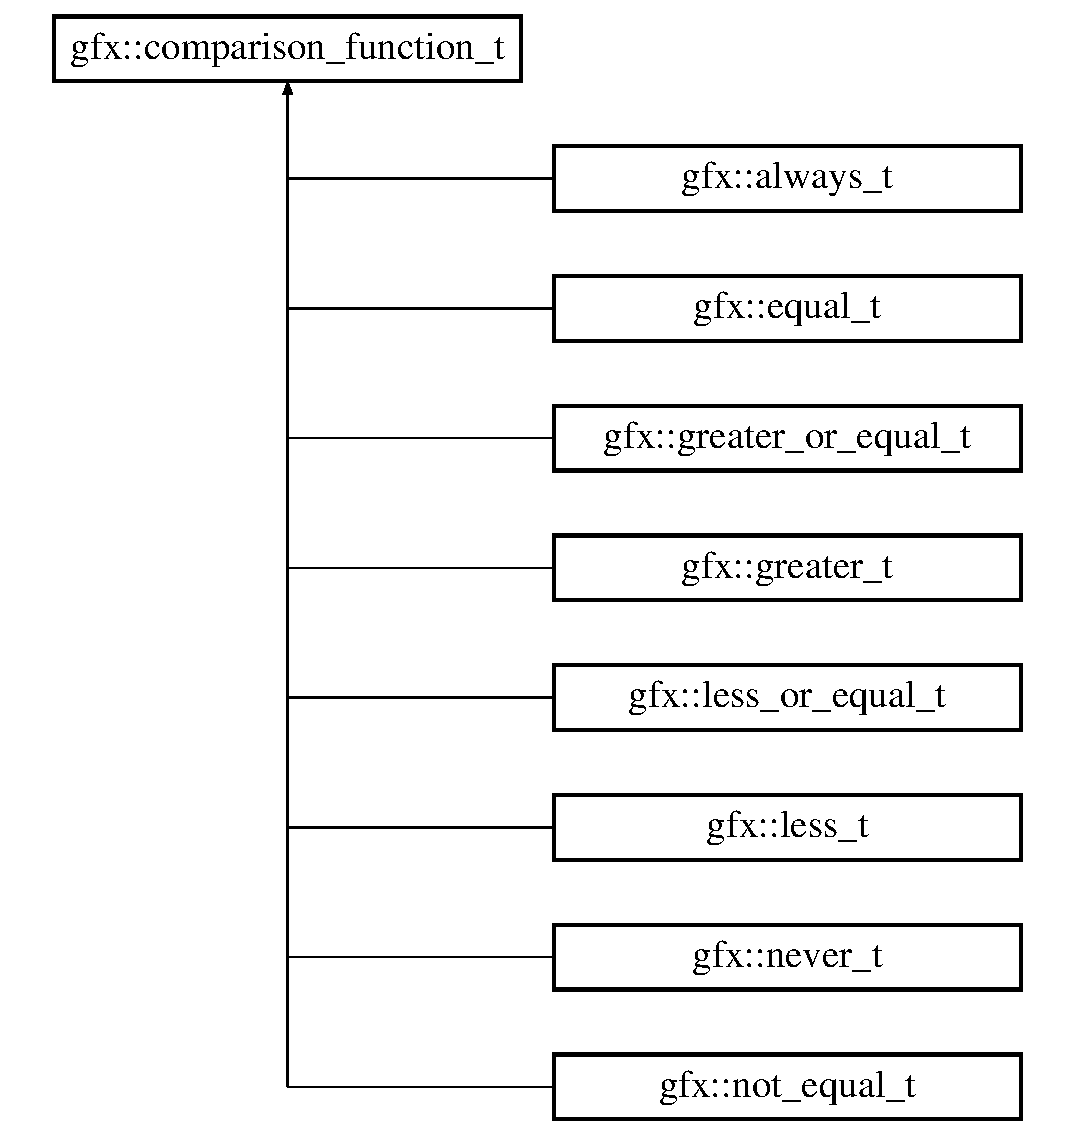
\includegraphics[height=9.000000cm]{classgfx_1_1comparison__function__t}
\end{center}
\end{figure}
\subsection*{Protected Member Functions}
\begin{DoxyCompactItemize}
\item 
\hypertarget{classgfx_1_1comparison__function__t_a173213f45db0d1b518d6b7950517755e}{virtual G\-Lint {\bfseries val} () const =0}\label{classgfx_1_1comparison__function__t_a173213f45db0d1b518d6b7950517755e}

\end{DoxyCompactItemize}
\subsection*{Friends}
\begin{DoxyCompactItemize}
\item 
\hypertarget{classgfx_1_1comparison__function__t_a2039d67f6166ccf823c78e3476aad9aa}{class {\bfseries texture\-\_\-1\-D}}\label{classgfx_1_1comparison__function__t_a2039d67f6166ccf823c78e3476aad9aa}

\item 
\hypertarget{classgfx_1_1comparison__function__t_a22ad86ef46c3b17357a0cd59e50bc7dd}{class {\bfseries texture\-\_\-2\-D}}\label{classgfx_1_1comparison__function__t_a22ad86ef46c3b17357a0cd59e50bc7dd}

\end{DoxyCompactItemize}


\subsection{Detailed Description}
Base class for comparison function selectors. 

An interface for comparison function selectors; there is no multiple inheritance in this class hierarachy, the derived classes are also the terminal ones. 

The documentation for this class was generated from the following file\-:\begin{DoxyCompactItemize}
\item 
g\-Scene/texture.\-hpp\end{DoxyCompactItemize}

\hypertarget{classgfx_1_1compilation__error}{\section{gfx\-:\-:compilation\-\_\-error Class Reference}
\label{classgfx_1_1compilation__error}\index{gfx\-::compilation\-\_\-error@{gfx\-::compilation\-\_\-error}}
}
Inheritance diagram for gfx\-:\-:compilation\-\_\-error\-:\begin{figure}[H]
\begin{center}
\leavevmode
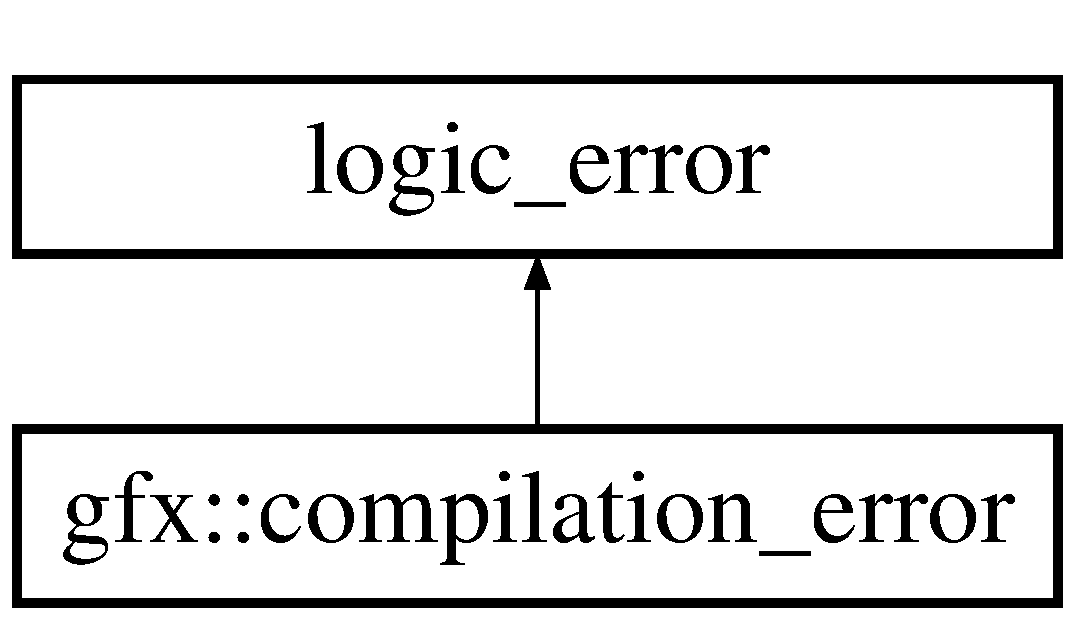
\includegraphics[height=2.000000cm]{classgfx_1_1compilation__error}
\end{center}
\end{figure}
\subsection*{Public Member Functions}
\begin{DoxyCompactItemize}
\item 
\hypertarget{classgfx_1_1compilation__error_a6b7152978001a084063277f327710512}{{\bfseries compilation\-\_\-error} (std\-::string const \&msg)}\label{classgfx_1_1compilation__error_a6b7152978001a084063277f327710512}

\end{DoxyCompactItemize}


The documentation for this class was generated from the following file\-:\begin{DoxyCompactItemize}
\item 
g\-Video/gfx\-\_\-exception.\-hpp\end{DoxyCompactItemize}

\hypertarget{classgfx_1_1context}{\section{gfx\-:\-:context Class Reference}
\label{classgfx_1_1context}\index{gfx\-::context@{gfx\-::context}}
}


Represents an Open\-G\-L rendering context.  




{\ttfamily \#include \char`\"{}g\-Core/g\-Video/context.\-hp\char`\"{}}

\subsection*{Classes}
\begin{DoxyCompactItemize}
\item 
class \hyperlink{classgfx_1_1context_1_1settings}{settings}
\begin{DoxyCompactList}\small\item\em Used to configure a \hyperlink{classgfx_1_1context}{context}. \end{DoxyCompactList}\end{DoxyCompactItemize}
\subsection*{Public Types}
\begin{DoxyCompactItemize}
\item 
\hypertarget{classgfx_1_1context_a8b1f7ba6e8a44dd16078d4084eef50ff}{typedef std\-::vector$<$ G\-Lubyte $>$ {\bfseries ub\-\_\-indexer}}\label{classgfx_1_1context_a8b1f7ba6e8a44dd16078d4084eef50ff}

\item 
\hypertarget{classgfx_1_1context_ae58ebbe469b3a22bf3e66ea7908cb877}{typedef std\-::vector$<$ G\-Lushort $>$ {\bfseries us\-\_\-indexer}}\label{classgfx_1_1context_ae58ebbe469b3a22bf3e66ea7908cb877}

\item 
\hypertarget{classgfx_1_1context_ac1f08fb34b7dad45044044611a76ec0c}{typedef std\-::vector$<$ G\-Luint $>$ {\bfseries ui\-\_\-indexer}}\label{classgfx_1_1context_ac1f08fb34b7dad45044044611a76ec0c}

\end{DoxyCompactItemize}
\subsection*{Public Member Functions}
\begin{DoxyCompactItemize}
\item 
\hyperlink{classgfx_1_1context_a7994d7183d5febf0b66f8e574d172180}{context} (\hyperlink{classgfx_1_1window}{window} const \&target\-\_\-window, \hyperlink{classgfx_1_1context_1_1settings}{settings} const \&set=\hyperlink{classgfx_1_1context_1_1settings}{settings}())
\begin{DoxyCompactList}\small\item\em Construct a new \hyperlink{classgfx_1_1context}{gfx\-::context} targeting the given window with the given settings. \end{DoxyCompactList}\item 
\hyperlink{classgfx_1_1context_a02588dfb533acd93bab925211bb48273}{$\sim$context} ()
\begin{DoxyCompactList}\small\item\em Destruct the \hyperlink{classgfx_1_1context}{context} object. \end{DoxyCompactList}\item 
void \hyperlink{classgfx_1_1context_abd71c661a4eaf846a10b15ad36e2b117}{clear\-\_\-color} (float red, float green, float blue, float alpha=1.\-0f)
\begin{DoxyCompactList}\small\item\em Clear the \hyperlink{classgfx_1_1context}{context's} framebuffer to the given color. \end{DoxyCompactList}\item 
bool \hyperlink{classgfx_1_1context_a49cbe1635efb5446884361c883b9756e}{is\-\_\-active} () const 
\begin{DoxyCompactList}\small\item\em Query the \hyperlink{classgfx_1_1context}{context} if it is the active context. \end{DoxyCompactList}\item 
unsigned int \hyperlink{classgfx_1_1context_aa16d73f975660c691ec1b23d2b357838}{major\-\_\-version} () const 
\begin{DoxyCompactList}\small\item\em Query the \hyperlink{classgfx_1_1context}{context} for the major version of the context. \end{DoxyCompactList}\item 
unsigned int \hyperlink{classgfx_1_1context_a42b72fb029aab81096e576b3a8a7de52}{minor\-\_\-version} () const 
\begin{DoxyCompactList}\small\item\em Query the \hyperlink{classgfx_1_1context}{context} for the minor version of the context. \end{DoxyCompactList}\item 
uvec2 \hyperlink{classgfx_1_1context_ab8ca4b7f55d6a658f08db1078781e4ba}{version} () const 
\begin{DoxyCompactList}\small\item\em Query the \hyperlink{classgfx_1_1context}{context} for the version of the context. \end{DoxyCompactList}\item 
unsigned int \hyperlink{classgfx_1_1context_ac56da3c0c0c6ebf4bd12462a21ed62c4}{depth\-\_\-bits} () const 
\begin{DoxyCompactList}\small\item\em Query the \hyperlink{classgfx_1_1context}{context} for the number of depth bits it uses. \end{DoxyCompactList}\item 
bool \hyperlink{classgfx_1_1context_ab74649cd35aee6e49a03ec6e31f97ee2}{double\-\_\-buffered} () const 
\begin{DoxyCompactList}\small\item\em Query the \hyperlink{classgfx_1_1context}{context} whether or not it uses double buffering. \end{DoxyCompactList}\item 
bool \hyperlink{classgfx_1_1context_a3004cb783117e15e03e477ab7660657a}{operator==} (\hyperlink{classgfx_1_1context}{context} const \&rhs) const 
\begin{DoxyCompactList}\small\item\em Compare this \hyperlink{classgfx_1_1context}{context} to another for equality. \end{DoxyCompactList}\item 
void \hyperlink{classgfx_1_1context_aaef26684c1625beaea62af3f1b6aefd2}{draw\-\_\-triangles} (size\-\_\-t const tris, ui\-\_\-indexer const \&indices)
\begin{DoxyCompactList}\small\item\em Draw triangles using the indices given. \end{DoxyCompactList}\end{DoxyCompactItemize}
\subsection*{Friends}
\begin{DoxyCompactItemize}
\item 
\hypertarget{classgfx_1_1context_abfd69a86b028655cf7807981b1c58526}{class {\bfseries video\-\_\-system}}\label{classgfx_1_1context_abfd69a86b028655cf7807981b1c58526}

\end{DoxyCompactItemize}


\subsection{Detailed Description}
Represents an Open\-G\-L rendering context. 

The way in which contexts and windows interact is obscure; It is possible that some Open\-G\-L settings need to be saved in order to make this all work correctly.

The context class is a representation of an Open\-G\-L rendering context. A valid context and associated \hyperlink{classgfx_1_1window}{window} are needed to render using Open\-G\-L, and an initialized \hyperlink{classgfx_1_1video__system}{video system} must be present. Some tedious details are handled automagically and configuration uses the \hyperlink{classgfx_1_1context_1_1settings}{settings member class}.

\begin{DoxyRefDesc}{Todo}
\item[\hyperlink{todo__todo000006}{Todo}]Review interaction with the window class. The way in which the two interact is obscure; it is possible that some Open\-G\-L settings need to be saved in order to make this all work correctly.\end{DoxyRefDesc}


\begin{DoxySeeAlso}{See Also}
\hyperlink{classgfx_1_1window}{gfx\-::window} 
\end{DoxySeeAlso}


\subsection{Constructor \& Destructor Documentation}
\hypertarget{classgfx_1_1context_a7994d7183d5febf0b66f8e574d172180}{\index{gfx\-::context@{gfx\-::context}!context@{context}}
\index{context@{context}!gfx::context@{gfx\-::context}}
\subsubsection[{context}]{\setlength{\rightskip}{0pt plus 5cm}gfx\-::context\-::context (
\begin{DoxyParamCaption}
\item[{{\bf window} const \&}]{window, }
\item[{{\bf settings} const \&}]{set = {\ttfamily {\bf settings}()}}
\end{DoxyParamCaption}
)}}\label{classgfx_1_1context_a7994d7183d5febf0b66f8e574d172180}


Construct a new \hyperlink{classgfx_1_1context}{gfx\-::context} targeting the given window with the given settings. 


\begin{DoxyParams}{Parameters}
{\em window} & The target window for the context \\
\hline
{\em set} & The settings for the new context \\
\hline
\end{DoxyParams}

\begin{DoxyExceptions}{Exceptions}
{\em std\-::logic\-\_\-error} & If the given window does not support Open\-G\-L, a standard logic error is thrown. \\
\hline
\end{DoxyExceptions}
\hypertarget{classgfx_1_1context_a02588dfb533acd93bab925211bb48273}{\index{gfx\-::context@{gfx\-::context}!$\sim$context@{$\sim$context}}
\index{$\sim$context@{$\sim$context}!gfx::context@{gfx\-::context}}
\subsubsection[{$\sim$context}]{\setlength{\rightskip}{0pt plus 5cm}gfx\-::context\-::$\sim$context (
\begin{DoxyParamCaption}
{}
\end{DoxyParamCaption}
)}}\label{classgfx_1_1context_a02588dfb533acd93bab925211bb48273}


Destruct the \hyperlink{classgfx_1_1context}{context} object. 

\begin{DoxyRefDesc}{Todo}
\item[\hyperlink{todo__todo000002}{Todo}]Review the 'zombie flag'. \end{DoxyRefDesc}


\subsection{Member Function Documentation}
\hypertarget{classgfx_1_1context_abd71c661a4eaf846a10b15ad36e2b117}{\index{gfx\-::context@{gfx\-::context}!clear\-\_\-color@{clear\-\_\-color}}
\index{clear\-\_\-color@{clear\-\_\-color}!gfx::context@{gfx\-::context}}
\subsubsection[{clear\-\_\-color}]{\setlength{\rightskip}{0pt plus 5cm}void gfx\-::context\-::clear\-\_\-color (
\begin{DoxyParamCaption}
\item[{float}]{red, }
\item[{float}]{green, }
\item[{float}]{blue, }
\item[{float}]{alpha = {\ttfamily 1.0f}}
\end{DoxyParamCaption}
)}}\label{classgfx_1_1context_abd71c661a4eaf846a10b15ad36e2b117}


Clear the \hyperlink{classgfx_1_1context}{context's} framebuffer to the given color. 


\begin{DoxyParams}{Parameters}
{\em red} & The value of the red chanel, normalized on \mbox{[}0.\-0f, 1.\-0f\mbox{]} \\
\hline
{\em green} & The value of the green chanel, normalized on \mbox{[}0.\-0f, 1.\-0f\mbox{]} \\
\hline
{\em blue} & The value of the blue chanel, normalized on \mbox{[}0.\-0f, 1.\-0f\mbox{]} \\
\hline
{\em alpha} & The value of the alpha chanel, normalized on \mbox{[}0.\-0f, 1.\-0f\mbox{]} \\
\hline
\end{DoxyParams}

\begin{DoxyExceptions}{Exceptions}
{\em std\-::logic\-\_\-error} & If the context is not the active context, a standard logic error is thrown. \\
\hline
\end{DoxyExceptions}
\hypertarget{classgfx_1_1context_ac56da3c0c0c6ebf4bd12462a21ed62c4}{\index{gfx\-::context@{gfx\-::context}!depth\-\_\-bits@{depth\-\_\-bits}}
\index{depth\-\_\-bits@{depth\-\_\-bits}!gfx::context@{gfx\-::context}}
\subsubsection[{depth\-\_\-bits}]{\setlength{\rightskip}{0pt plus 5cm}unsigned int gfx\-::context\-::depth\-\_\-bits (
\begin{DoxyParamCaption}
{}
\end{DoxyParamCaption}
) const}}\label{classgfx_1_1context_ac56da3c0c0c6ebf4bd12462a21ed62c4}


Query the \hyperlink{classgfx_1_1context}{context} for the number of depth bits it uses. 

\begin{DoxyReturn}{Returns}
The number of dpeth bits the context uses 
\end{DoxyReturn}

\begin{DoxyExceptions}{Exceptions}
{\em std\-::logic\-\_\-error} & Calling this function on a context that is not the active one generates a standard logic error. \\
\hline
{\em std\-::runtime\-\_\-error} & If, for some reason, the query fails, a standard runtime error will be thrwon. \\
\hline
\end{DoxyExceptions}
\hypertarget{classgfx_1_1context_ab74649cd35aee6e49a03ec6e31f97ee2}{\index{gfx\-::context@{gfx\-::context}!double\-\_\-buffered@{double\-\_\-buffered}}
\index{double\-\_\-buffered@{double\-\_\-buffered}!gfx::context@{gfx\-::context}}
\subsubsection[{double\-\_\-buffered}]{\setlength{\rightskip}{0pt plus 5cm}bool gfx\-::context\-::double\-\_\-buffered (
\begin{DoxyParamCaption}
{}
\end{DoxyParamCaption}
) const}}\label{classgfx_1_1context_ab74649cd35aee6e49a03ec6e31f97ee2}


Query the \hyperlink{classgfx_1_1context}{context} whether or not it uses double buffering. 

\begin{DoxyReturn}{Returns}
Whether the context uses double buffering 
\end{DoxyReturn}

\begin{DoxyExceptions}{Exceptions}
{\em std\-::logic\-\_\-error} & Calling this function on a context that is not the active one generates a standard logic error. \\
\hline
{\em std\-::runtime\-\_\-error} & If, for some reason, the query fails, a standard runtime error will be thrwon. \\
\hline
\end{DoxyExceptions}
\hypertarget{classgfx_1_1context_aaef26684c1625beaea62af3f1b6aefd2}{\index{gfx\-::context@{gfx\-::context}!draw\-\_\-triangles@{draw\-\_\-triangles}}
\index{draw\-\_\-triangles@{draw\-\_\-triangles}!gfx::context@{gfx\-::context}}
\subsubsection[{draw\-\_\-triangles}]{\setlength{\rightskip}{0pt plus 5cm}void gfx\-::context\-::draw\-\_\-triangles (
\begin{DoxyParamCaption}
\item[{size\-\_\-t const}]{tris, }
\item[{ui\-\_\-indexer const \&}]{indices}
\end{DoxyParamCaption}
)\hspace{0.3cm}{\ttfamily [inline]}}}\label{classgfx_1_1context_aaef26684c1625beaea62af3f1b6aefd2}


Draw triangles using the indices given. 

This is a trainwreck of badness; it is only a placeholder and I don't even know if it works (I strongly suspect it does not). It requires a vertex array object and associated buffer to be active before it works. 
\begin{DoxyParams}{Parameters}
{\em tris} & The number of triangles the given indexer describes \\
\hline
{\em indices} & The indices that describe the triangles. \\
\hline
\end{DoxyParams}
\hypertarget{classgfx_1_1context_a49cbe1635efb5446884361c883b9756e}{\index{gfx\-::context@{gfx\-::context}!is\-\_\-active@{is\-\_\-active}}
\index{is\-\_\-active@{is\-\_\-active}!gfx::context@{gfx\-::context}}
\subsubsection[{is\-\_\-active}]{\setlength{\rightskip}{0pt plus 5cm}bool gfx\-::context\-::is\-\_\-active (
\begin{DoxyParamCaption}
{}
\end{DoxyParamCaption}
) const}}\label{classgfx_1_1context_a49cbe1635efb5446884361c883b9756e}


Query the \hyperlink{classgfx_1_1context}{context} if it is the active context. 

\begin{DoxyReturn}{Returns}
Whether or not the context is active. 
\end{DoxyReturn}
\hypertarget{classgfx_1_1context_aa16d73f975660c691ec1b23d2b357838}{\index{gfx\-::context@{gfx\-::context}!major\-\_\-version@{major\-\_\-version}}
\index{major\-\_\-version@{major\-\_\-version}!gfx::context@{gfx\-::context}}
\subsubsection[{major\-\_\-version}]{\setlength{\rightskip}{0pt plus 5cm}unsigned int gfx\-::context\-::major\-\_\-version (
\begin{DoxyParamCaption}
{}
\end{DoxyParamCaption}
) const}}\label{classgfx_1_1context_aa16d73f975660c691ec1b23d2b357838}


Query the \hyperlink{classgfx_1_1context}{context} for the major version of the context. 

\begin{DoxyRefDesc}{Todo}
\item[\hyperlink{todo__todo000003}{Todo}]Why do we even need this? Review for removal. \begin{DoxyReturn}{Returns}
The major version number of the context. 
\end{DoxyReturn}

\begin{DoxyExceptions}{Exceptions}
{\em std\-::logic\-\_\-error} & Calling this function on a context that is not the active one generates a standard logic error. \\
\hline
{\em std\-::runtime\-\_\-error} & If, for some reason, the query fails, a standard runtime error will be thrwon. \\
\hline
\end{DoxyExceptions}
\end{DoxyRefDesc}
\hypertarget{classgfx_1_1context_a42b72fb029aab81096e576b3a8a7de52}{\index{gfx\-::context@{gfx\-::context}!minor\-\_\-version@{minor\-\_\-version}}
\index{minor\-\_\-version@{minor\-\_\-version}!gfx::context@{gfx\-::context}}
\subsubsection[{minor\-\_\-version}]{\setlength{\rightskip}{0pt plus 5cm}unsigned int gfx\-::context\-::minor\-\_\-version (
\begin{DoxyParamCaption}
{}
\end{DoxyParamCaption}
) const}}\label{classgfx_1_1context_a42b72fb029aab81096e576b3a8a7de52}


Query the \hyperlink{classgfx_1_1context}{context} for the minor version of the context. 

\begin{DoxyRefDesc}{Todo}
\item[\hyperlink{todo__todo000004}{Todo}]Why do we even need this? Review for removal. \begin{DoxyReturn}{Returns}
The minor version number of the context. 
\end{DoxyReturn}

\begin{DoxyExceptions}{Exceptions}
{\em std\-::logic\-\_\-error} & Calling this function on a context that is not the active one generates a standard logic error. \\
\hline
{\em std\-::runtime\-\_\-error} & If, for some reason, the query fails, a standard runtime error will be thrwon. \\
\hline
\end{DoxyExceptions}
\end{DoxyRefDesc}
\hypertarget{classgfx_1_1context_a3004cb783117e15e03e477ab7660657a}{\index{gfx\-::context@{gfx\-::context}!operator==@{operator==}}
\index{operator==@{operator==}!gfx::context@{gfx\-::context}}
\subsubsection[{operator==}]{\setlength{\rightskip}{0pt plus 5cm}bool gfx\-::context\-::operator== (
\begin{DoxyParamCaption}
\item[{{\bf context} const \&}]{rhs}
\end{DoxyParamCaption}
) const\hspace{0.3cm}{\ttfamily [inline]}}}\label{classgfx_1_1context_a3004cb783117e15e03e477ab7660657a}


Compare this \hyperlink{classgfx_1_1context}{context} to another for equality. 

The comparison is down using internal Open\-G\-L system values; it is feasible that two contexts could compare equal, but extremely extremely unlikely as it would require ill-\/advised hacking of how the \hyperlink{classgfx_1_1video__system}{video system} works. 
\begin{DoxyParams}{Parameters}
{\em rhs} & The context to compare this context to \\
\hline
\end{DoxyParams}
\hypertarget{classgfx_1_1context_ab8ca4b7f55d6a658f08db1078781e4ba}{\index{gfx\-::context@{gfx\-::context}!version@{version}}
\index{version@{version}!gfx::context@{gfx\-::context}}
\subsubsection[{version}]{\setlength{\rightskip}{0pt plus 5cm}uvec2 gfx\-::context\-::version (
\begin{DoxyParamCaption}
{}
\end{DoxyParamCaption}
) const}}\label{classgfx_1_1context_ab8ca4b7f55d6a658f08db1078781e4ba}


Query the \hyperlink{classgfx_1_1context}{context} for the version of the context. 

\begin{DoxyRefDesc}{Todo}
\item[\hyperlink{todo__todo000005}{Todo}]Why do we even need this? Review for removal. If it is kept, then change the return type to a \hyperlink{classgfx_1_1version}{version} object. \begin{DoxyReturn}{Returns}
The version number of the context, represented as a vec2 
\end{DoxyReturn}

\begin{DoxyExceptions}{Exceptions}
{\em std\-::logic\-\_\-error} & Calling this function on a context that is not the active one generates a standard logic error. \\
\hline
{\em std\-::runtime\-\_\-error} & If, for some reason, the query fails, a standard runtime error will be thrwon. \\
\hline
\end{DoxyExceptions}
\end{DoxyRefDesc}


The documentation for this class was generated from the following files\-:\begin{DoxyCompactItemize}
\item 
g\-Video/context.\-hpp\item 
g\-Video/context.\-cpp\end{DoxyCompactItemize}

\hypertarget{classgfx_1_1eight__bit__t}{\section{gfx\-:\-:eight\-\_\-bit\-\_\-t Class Reference}
\label{classgfx_1_1eight__bit__t}\index{gfx\-::eight\-\_\-bit\-\_\-t@{gfx\-::eight\-\_\-bit\-\_\-t}}
}


Selects for eight bit channel formats.  




{\ttfamily \#include \char`\"{}g\-Core/g\-Scene/texture.\-hpp\char`\"{}}

Inheritance diagram for gfx\-:\-:eight\-\_\-bit\-\_\-t\-:\begin{figure}[H]
\begin{center}
\leavevmode
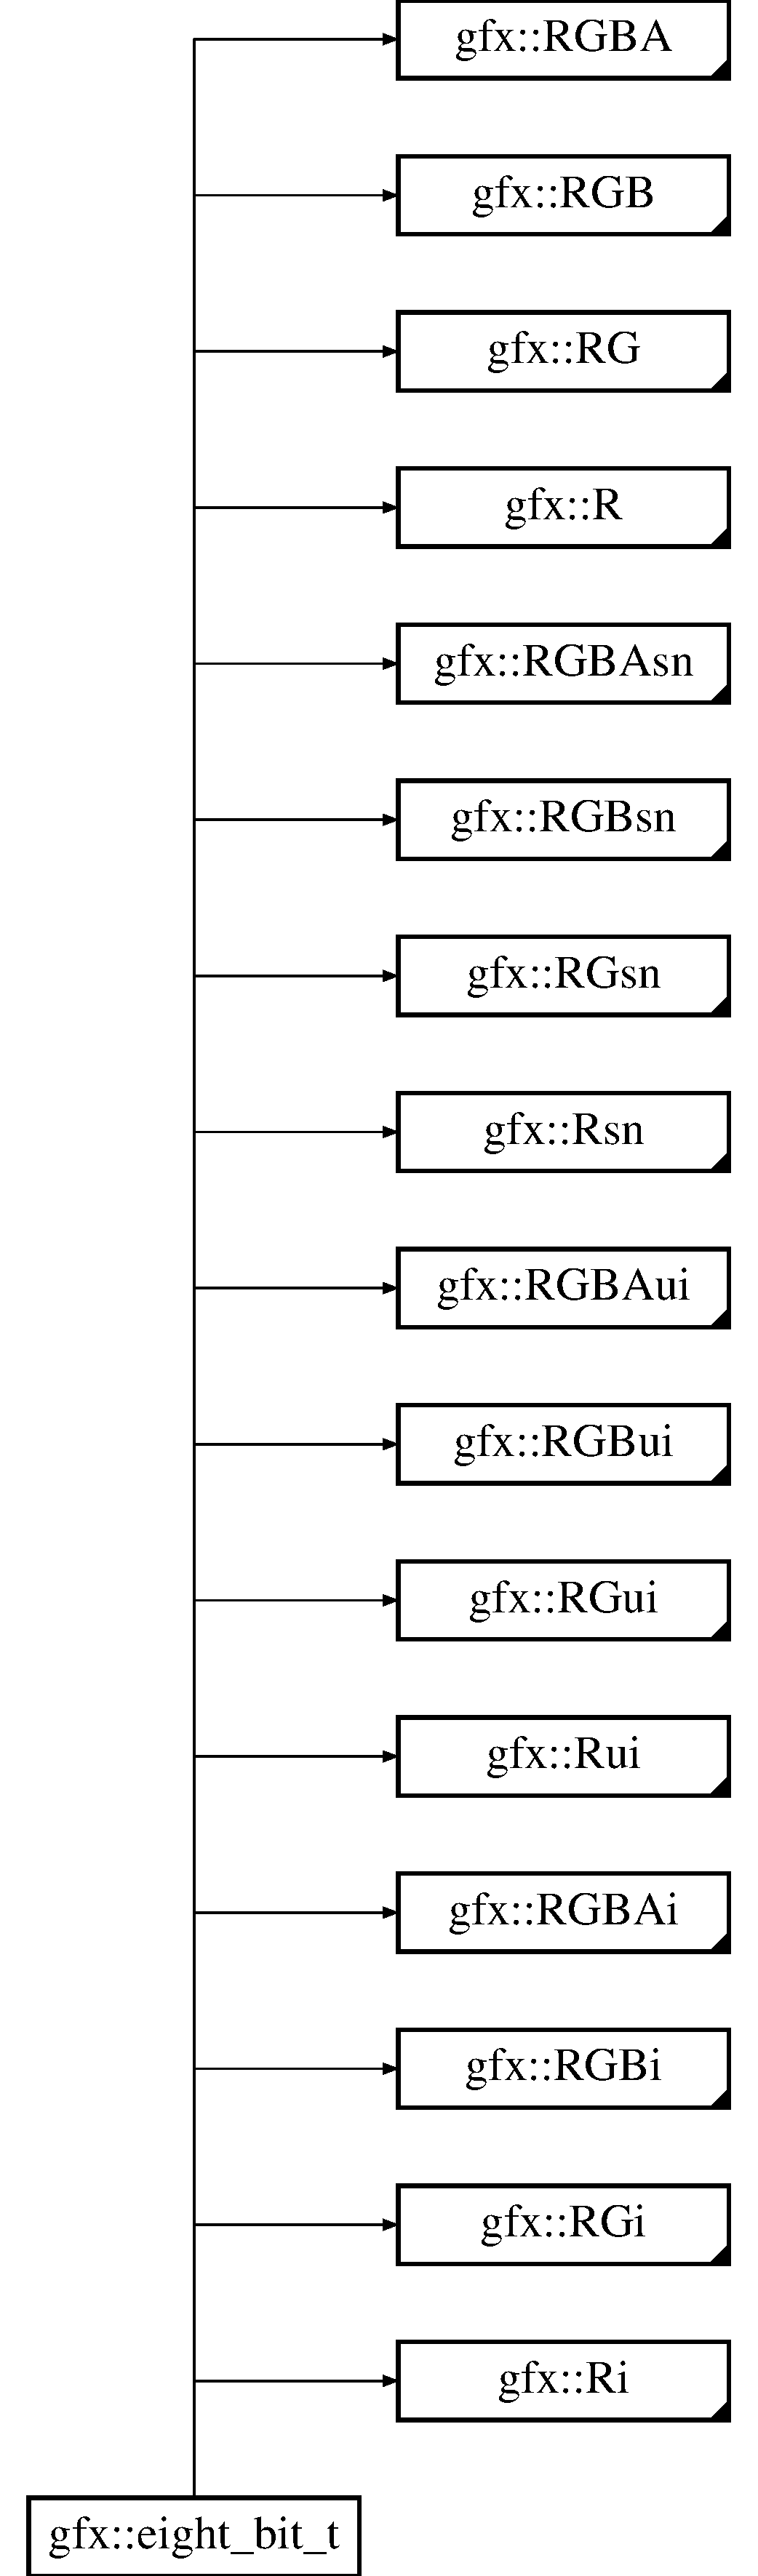
\includegraphics[height=12.000000cm]{classgfx_1_1eight__bit__t}
\end{center}
\end{figure}
\subsection*{Public Member Functions}
\begin{DoxyCompactItemize}
\item 
\hypertarget{classgfx_1_1eight__bit__t_a9ea91348fcffdae6153e2f5ab6953bdc}{virtual size\-\_\-t {\bfseries n} () const }\label{classgfx_1_1eight__bit__t_a9ea91348fcffdae6153e2f5ab6953bdc}

\end{DoxyCompactItemize}


\subsection{Detailed Description}
Selects for eight bit channel formats. 

The documentation for this class was generated from the following file\-:\begin{DoxyCompactItemize}
\item 
g\-Scene/texture.\-hpp\end{DoxyCompactItemize}

\hypertarget{classgfx_1_1equal__t}{\section{gfx\-:\-:equal\-\_\-t Class Reference}
\label{classgfx_1_1equal__t}\index{gfx\-::equal\-\_\-t@{gfx\-::equal\-\_\-t}}
}


Selector for the equal to comparison function.  




{\ttfamily \#include \char`\"{}g\-Core/g\-Video/texture.\-hpp\char`\"{}}

Inheritance diagram for gfx\-:\-:equal\-\_\-t\-:\begin{figure}[H]
\begin{center}
\leavevmode
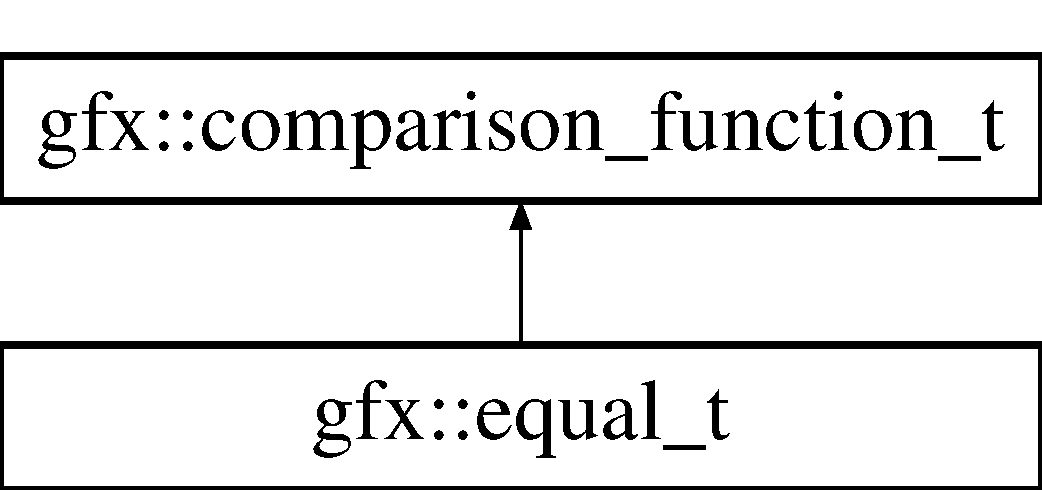
\includegraphics[height=2.000000cm]{classgfx_1_1equal__t}
\end{center}
\end{figure}
\subsection*{Protected Member Functions}
\begin{DoxyCompactItemize}
\item 
\hypertarget{classgfx_1_1equal__t_a86259aec05c6504aab05ac74424b146f}{virtual G\-Lint {\bfseries val} () const }\label{classgfx_1_1equal__t_a86259aec05c6504aab05ac74424b146f}

\end{DoxyCompactItemize}
\subsection*{Friends}
\begin{DoxyCompactItemize}
\item 
\hypertarget{classgfx_1_1equal__t_a2039d67f6166ccf823c78e3476aad9aa}{class {\bfseries texture\-\_\-1\-D}}\label{classgfx_1_1equal__t_a2039d67f6166ccf823c78e3476aad9aa}

\item 
\hypertarget{classgfx_1_1equal__t_a22ad86ef46c3b17357a0cd59e50bc7dd}{class {\bfseries texture\-\_\-2\-D}}\label{classgfx_1_1equal__t_a22ad86ef46c3b17357a0cd59e50bc7dd}

\end{DoxyCompactItemize}


\subsection{Detailed Description}
Selector for the equal to comparison function. 

The documentation for this class was generated from the following file\-:\begin{DoxyCompactItemize}
\item 
g\-Scene/texture.\-hpp\end{DoxyCompactItemize}

\hypertarget{classgfx_1_1filter__t}{\section{gfx\-:\-:filter\-\_\-t Class Reference}
\label{classgfx_1_1filter__t}\index{gfx\-::filter\-\_\-t@{gfx\-::filter\-\_\-t}}
}


Base class for interpolation filter selectors.  




{\ttfamily \#include \char`\"{}g\-Core/g\-Video/texture.\-hpp\char`\"{}}

Inheritance diagram for gfx\-:\-:filter\-\_\-t\-:\begin{figure}[H]
\begin{center}
\leavevmode
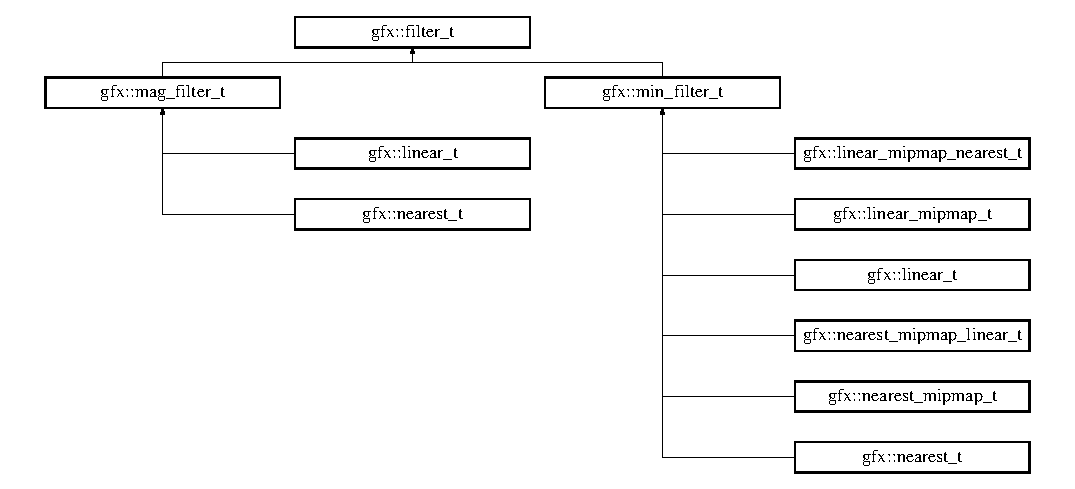
\includegraphics[height=6.120219cm]{classgfx_1_1filter__t}
\end{center}
\end{figure}
\subsection*{Protected Member Functions}
\begin{DoxyCompactItemize}
\item 
\hypertarget{classgfx_1_1filter__t_a131f10d9038f1ca5ac047e690ba7494e}{virtual G\-Lint {\bfseries val} () const =0}\label{classgfx_1_1filter__t_a131f10d9038f1ca5ac047e690ba7494e}

\end{DoxyCompactItemize}
\subsection*{Friends}
\begin{DoxyCompactItemize}
\item 
\hypertarget{classgfx_1_1filter__t_a2039d67f6166ccf823c78e3476aad9aa}{class {\bfseries texture\-\_\-1\-D}}\label{classgfx_1_1filter__t_a2039d67f6166ccf823c78e3476aad9aa}

\item 
\hypertarget{classgfx_1_1filter__t_a22ad86ef46c3b17357a0cd59e50bc7dd}{class {\bfseries texture\-\_\-2\-D}}\label{classgfx_1_1filter__t_a22ad86ef46c3b17357a0cd59e50bc7dd}

\end{DoxyCompactItemize}


\subsection{Detailed Description}
Base class for interpolation filter selectors. 

Interpolation selectors are used in the configuration of textures. Immediate derived classes of \hyperlink{classgfx_1_1filter__t}{filter\-\_\-t} are a family of classes that provide the terminal classes of the inheritance hierarchy with type signatures that ensure only legal filter types can be used for configuring a particular filter mode. 

The documentation for this class was generated from the following file\-:\begin{DoxyCompactItemize}
\item 
g\-Scene/texture.\-hpp\end{DoxyCompactItemize}

\hypertarget{classgfx_1_1five__bit__t}{\section{gfx\-:\-:five\-\_\-bit\-\_\-t Class Reference}
\label{classgfx_1_1five__bit__t}\index{gfx\-::five\-\_\-bit\-\_\-t@{gfx\-::five\-\_\-bit\-\_\-t}}
}


Selects for five bit channel formats.  




{\ttfamily \#include \char`\"{}g\-Core/g\-Scene/texture.\-hpp\char`\"{}}

Inheritance diagram for gfx\-:\-:five\-\_\-bit\-\_\-t\-:\begin{figure}[H]
\begin{center}
\leavevmode
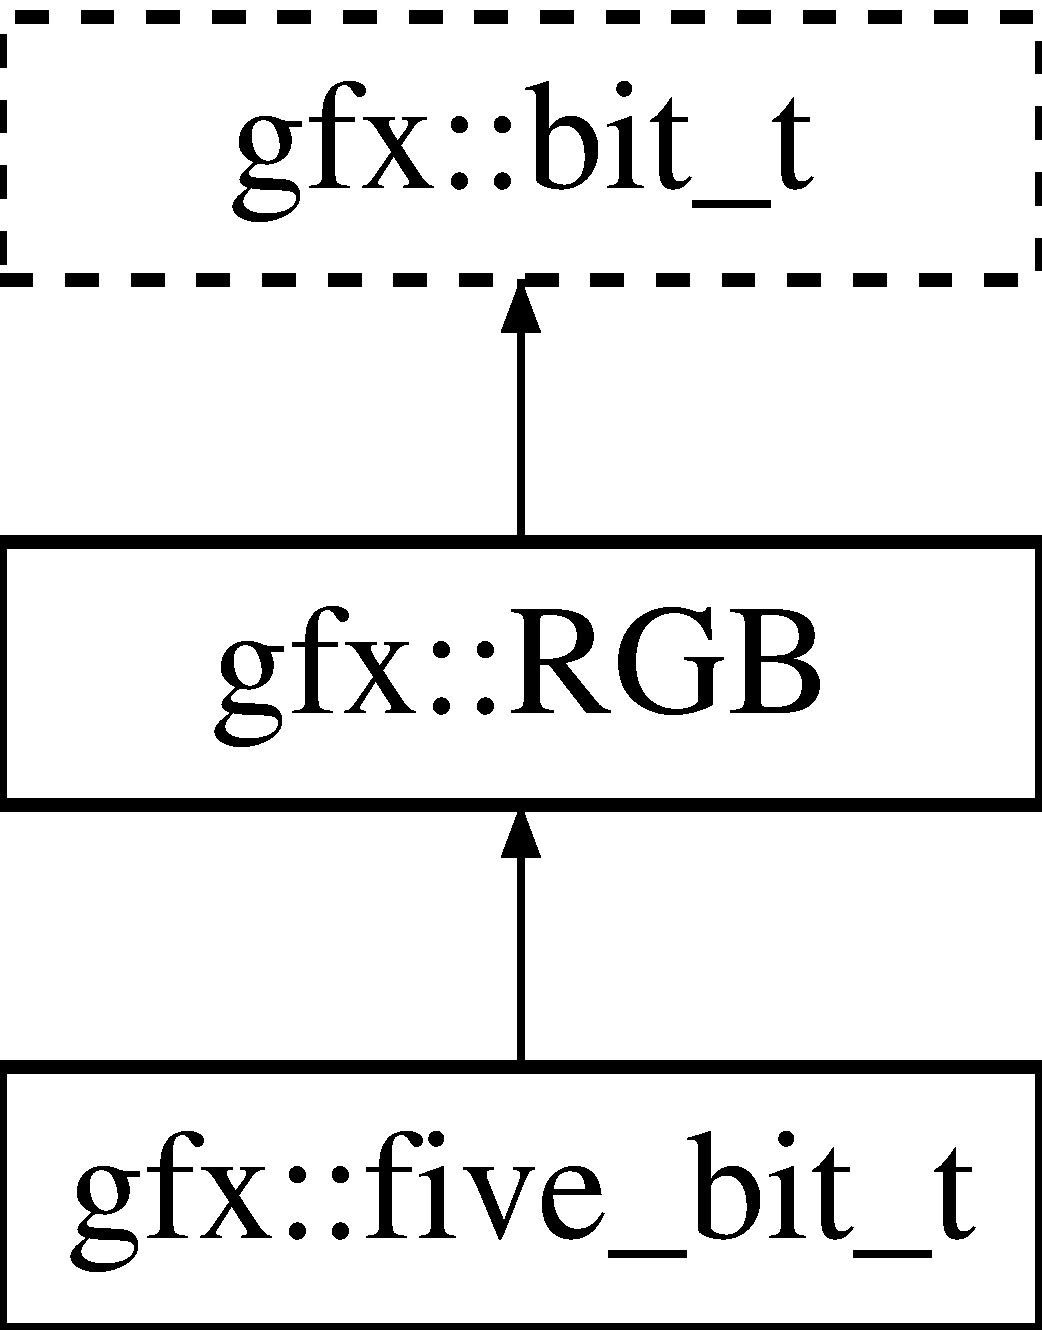
\includegraphics[height=3.000000cm]{classgfx_1_1five__bit__t}
\end{center}
\end{figure}
\subsection*{Public Member Functions}
\begin{DoxyCompactItemize}
\item 
\hypertarget{classgfx_1_1five__bit__t_a1a679bbd79e36d9f539f7dd566289880}{virtual size\-\_\-t {\bfseries n} () const }\label{classgfx_1_1five__bit__t_a1a679bbd79e36d9f539f7dd566289880}

\end{DoxyCompactItemize}


\subsection{Detailed Description}
Selects for five bit channel formats. 

The documentation for this class was generated from the following file\-:\begin{DoxyCompactItemize}
\item 
g\-Scene/texture.\-hpp\end{DoxyCompactItemize}

\hypertarget{classgfx_1_1four__bit__t}{\section{gfx\-:\-:four\-\_\-bit\-\_\-t Class Reference}
\label{classgfx_1_1four__bit__t}\index{gfx\-::four\-\_\-bit\-\_\-t@{gfx\-::four\-\_\-bit\-\_\-t}}
}


Selects for tour bit channel formats.  




{\ttfamily \#include \char`\"{}g\-Core/g\-Scene/texture.\-hpp\char`\"{}}

Inheritance diagram for gfx\-:\-:four\-\_\-bit\-\_\-t\-:\begin{figure}[H]
\begin{center}
\leavevmode
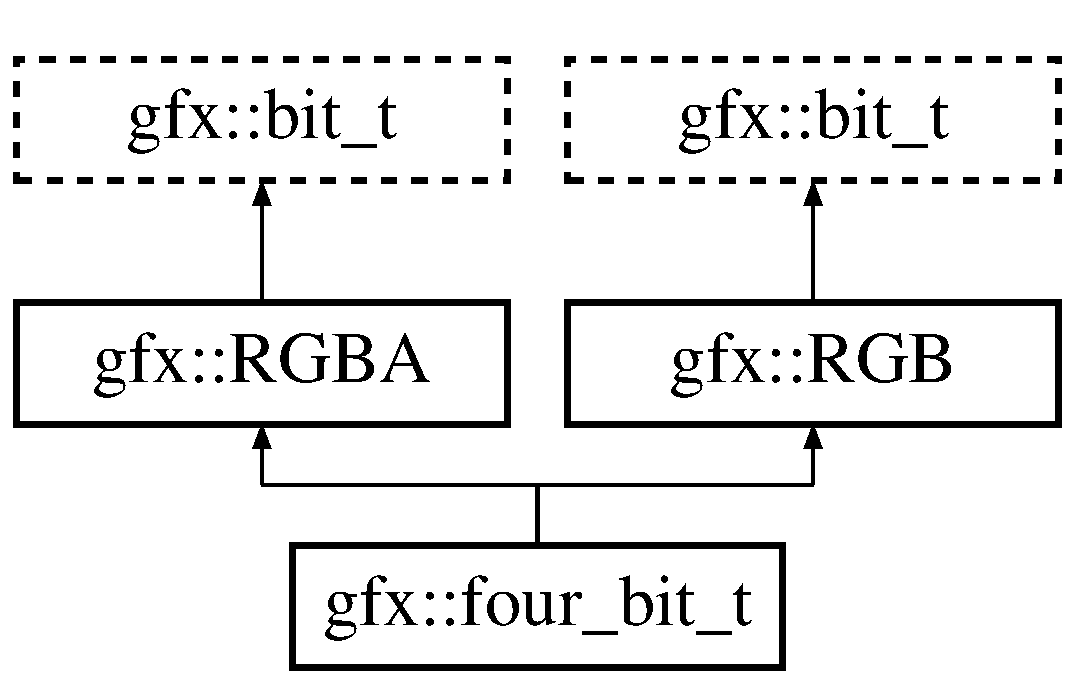
\includegraphics[height=3.000000cm]{classgfx_1_1four__bit__t}
\end{center}
\end{figure}
\subsection*{Public Member Functions}
\begin{DoxyCompactItemize}
\item 
\hypertarget{classgfx_1_1four__bit__t_a4ca51b6edea0b30a335a45d8f7eb3685}{virtual size\-\_\-t {\bfseries n} () const }\label{classgfx_1_1four__bit__t_a4ca51b6edea0b30a335a45d8f7eb3685}

\end{DoxyCompactItemize}


\subsection{Detailed Description}
Selects for tour bit channel formats. 

The documentation for this class was generated from the following file\-:\begin{DoxyCompactItemize}
\item 
g\-Scene/texture.\-hpp\end{DoxyCompactItemize}

\hypertarget{classgfx_1_1greater__or__equal__t}{\section{gfx\-:\-:greater\-\_\-or\-\_\-equal\-\_\-t Class Reference}
\label{classgfx_1_1greater__or__equal__t}\index{gfx\-::greater\-\_\-or\-\_\-equal\-\_\-t@{gfx\-::greater\-\_\-or\-\_\-equal\-\_\-t}}
}


Selector for the greater than or equal to comparison function.  




{\ttfamily \#include \char`\"{}g\-Core/g\-Video/texture.\-hpp\char`\"{}}

Inheritance diagram for gfx\-:\-:greater\-\_\-or\-\_\-equal\-\_\-t\-:\begin{figure}[H]
\begin{center}
\leavevmode
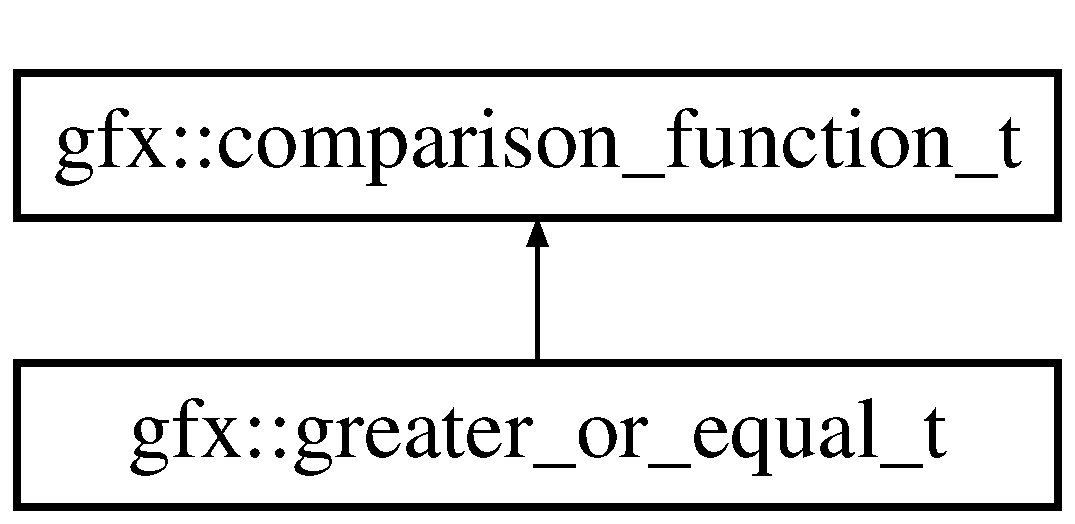
\includegraphics[height=2.000000cm]{classgfx_1_1greater__or__equal__t}
\end{center}
\end{figure}
\subsection*{Protected Member Functions}
\begin{DoxyCompactItemize}
\item 
\hypertarget{classgfx_1_1greater__or__equal__t_a6d61e5879883460be6ea338742cd2451}{virtual G\-Lint {\bfseries val} () const }\label{classgfx_1_1greater__or__equal__t_a6d61e5879883460be6ea338742cd2451}

\end{DoxyCompactItemize}
\subsection*{Friends}
\begin{DoxyCompactItemize}
\item 
\hypertarget{classgfx_1_1greater__or__equal__t_a2039d67f6166ccf823c78e3476aad9aa}{class {\bfseries texture\-\_\-1\-D}}\label{classgfx_1_1greater__or__equal__t_a2039d67f6166ccf823c78e3476aad9aa}

\item 
\hypertarget{classgfx_1_1greater__or__equal__t_a22ad86ef46c3b17357a0cd59e50bc7dd}{class {\bfseries texture\-\_\-2\-D}}\label{classgfx_1_1greater__or__equal__t_a22ad86ef46c3b17357a0cd59e50bc7dd}

\end{DoxyCompactItemize}


\subsection{Detailed Description}
Selector for the greater than or equal to comparison function. 

The documentation for this class was generated from the following file\-:\begin{DoxyCompactItemize}
\item 
g\-Scene/texture.\-hpp\end{DoxyCompactItemize}

\hypertarget{classgfx_1_1greater__t}{\section{gfx\-:\-:greater\-\_\-t Class Reference}
\label{classgfx_1_1greater__t}\index{gfx\-::greater\-\_\-t@{gfx\-::greater\-\_\-t}}
}


Selector for the greater than comparison function.  




{\ttfamily \#include \char`\"{}g\-Core/g\-Video/texture.\-hpp\char`\"{}}

Inheritance diagram for gfx\-:\-:greater\-\_\-t\-:\begin{figure}[H]
\begin{center}
\leavevmode
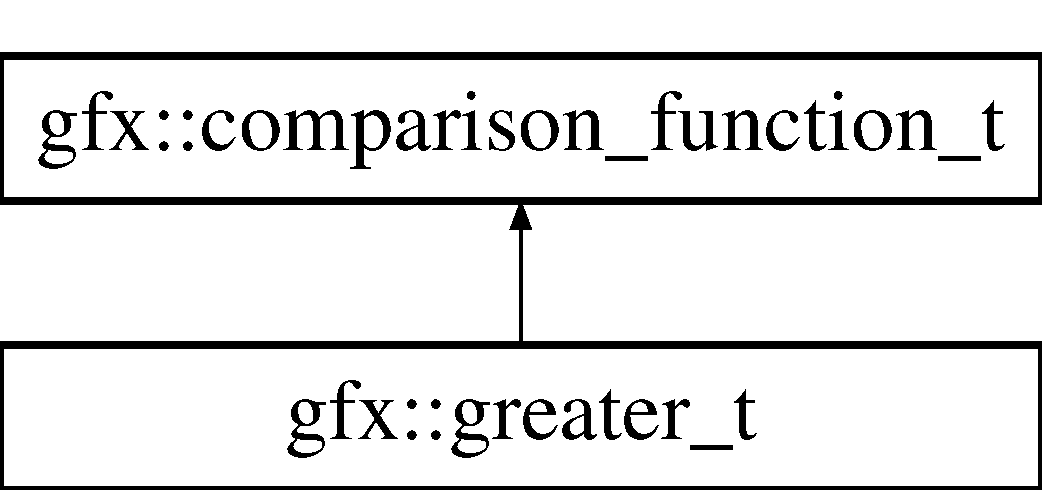
\includegraphics[height=2.000000cm]{classgfx_1_1greater__t}
\end{center}
\end{figure}
\subsection*{Protected Member Functions}
\begin{DoxyCompactItemize}
\item 
\hypertarget{classgfx_1_1greater__t_a98b69d70fefdcf5ea50811860928c1a4}{virtual G\-Lint {\bfseries val} () const }\label{classgfx_1_1greater__t_a98b69d70fefdcf5ea50811860928c1a4}

\end{DoxyCompactItemize}
\subsection*{Friends}
\begin{DoxyCompactItemize}
\item 
\hypertarget{classgfx_1_1greater__t_a2039d67f6166ccf823c78e3476aad9aa}{class {\bfseries texture\-\_\-1\-D}}\label{classgfx_1_1greater__t_a2039d67f6166ccf823c78e3476aad9aa}

\item 
\hypertarget{classgfx_1_1greater__t_a22ad86ef46c3b17357a0cd59e50bc7dd}{class {\bfseries texture\-\_\-2\-D}}\label{classgfx_1_1greater__t_a22ad86ef46c3b17357a0cd59e50bc7dd}

\end{DoxyCompactItemize}


\subsection{Detailed Description}
Selector for the greater than comparison function. 

The documentation for this class was generated from the following file\-:\begin{DoxyCompactItemize}
\item 
g\-Scene/texture.\-hpp\end{DoxyCompactItemize}

\hypertarget{classgfx_1_1initialization__error}{\section{gfx\-:\-:initialization\-\_\-error Class Reference}
\label{classgfx_1_1initialization__error}\index{gfx\-::initialization\-\_\-error@{gfx\-::initialization\-\_\-error}}
}
Inheritance diagram for gfx\-:\-:initialization\-\_\-error\-:\begin{figure}[H]
\begin{center}
\leavevmode
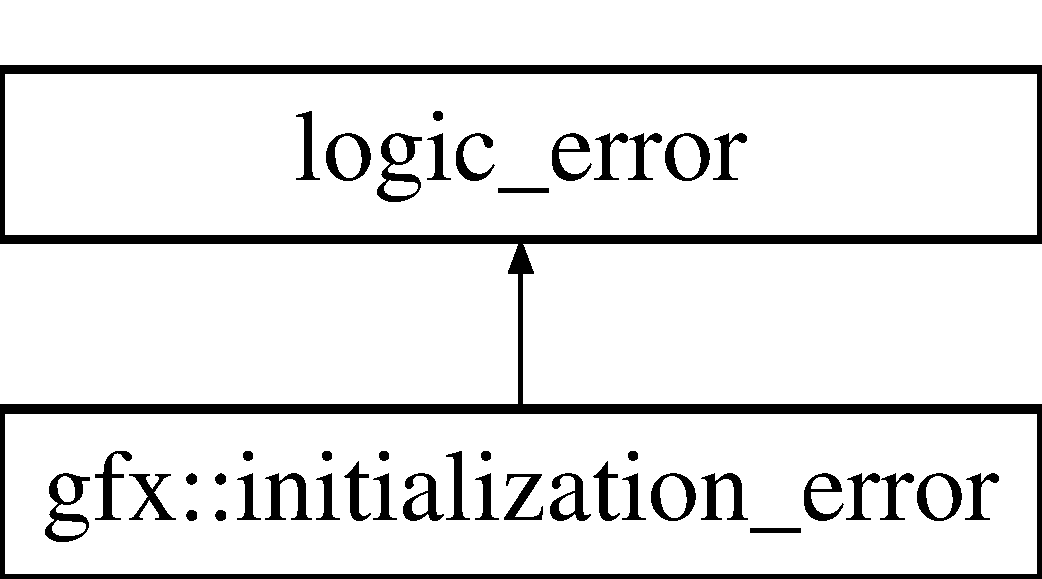
\includegraphics[height=2.000000cm]{classgfx_1_1initialization__error}
\end{center}
\end{figure}
\subsection*{Public Member Functions}
\begin{DoxyCompactItemize}
\item 
\hypertarget{classgfx_1_1initialization__error_a37bdd0e6006f04c19e2fb35fd3fb206c}{{\bfseries initialization\-\_\-error} (std\-::string const \&msg)}\label{classgfx_1_1initialization__error_a37bdd0e6006f04c19e2fb35fd3fb206c}

\end{DoxyCompactItemize}


The documentation for this class was generated from the following file\-:\begin{DoxyCompactItemize}
\item 
g\-Video/gfx\-\_\-exception.\-hpp\end{DoxyCompactItemize}

\hypertarget{classgfx_1_1less__or__equal__t}{\section{gfx\-:\-:less\-\_\-or\-\_\-equal\-\_\-t Class Reference}
\label{classgfx_1_1less__or__equal__t}\index{gfx\-::less\-\_\-or\-\_\-equal\-\_\-t@{gfx\-::less\-\_\-or\-\_\-equal\-\_\-t}}
}


Selector for the less than or equal to comparison function.  




{\ttfamily \#include \char`\"{}g\-Core/g\-Video/texture.\-hpp\char`\"{}}

Inheritance diagram for gfx\-:\-:less\-\_\-or\-\_\-equal\-\_\-t\-:\begin{figure}[H]
\begin{center}
\leavevmode
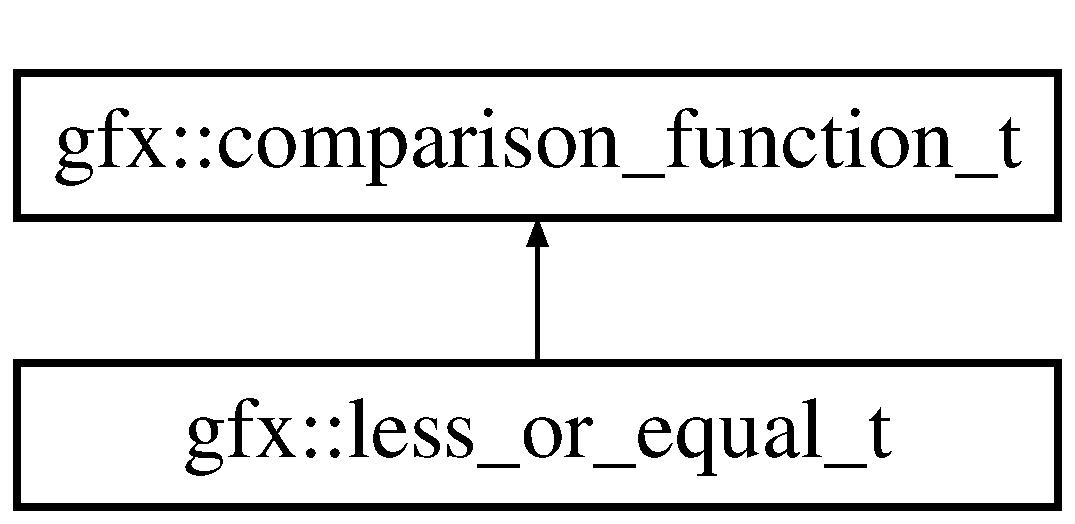
\includegraphics[height=2.000000cm]{classgfx_1_1less__or__equal__t}
\end{center}
\end{figure}
\subsection*{Protected Member Functions}
\begin{DoxyCompactItemize}
\item 
\hypertarget{classgfx_1_1less__or__equal__t_ab494c5a2a21f4d4777955e779447b058}{virtual G\-Lint {\bfseries val} () const }\label{classgfx_1_1less__or__equal__t_ab494c5a2a21f4d4777955e779447b058}

\end{DoxyCompactItemize}
\subsection*{Friends}
\begin{DoxyCompactItemize}
\item 
\hypertarget{classgfx_1_1less__or__equal__t_a2039d67f6166ccf823c78e3476aad9aa}{class {\bfseries texture\-\_\-1\-D}}\label{classgfx_1_1less__or__equal__t_a2039d67f6166ccf823c78e3476aad9aa}

\item 
\hypertarget{classgfx_1_1less__or__equal__t_a22ad86ef46c3b17357a0cd59e50bc7dd}{class {\bfseries texture\-\_\-2\-D}}\label{classgfx_1_1less__or__equal__t_a22ad86ef46c3b17357a0cd59e50bc7dd}

\end{DoxyCompactItemize}


\subsection{Detailed Description}
Selector for the less than or equal to comparison function. 

The documentation for this class was generated from the following file\-:\begin{DoxyCompactItemize}
\item 
g\-Scene/texture.\-hpp\end{DoxyCompactItemize}

\hypertarget{classgfx_1_1less__t}{\section{gfx\-:\-:less\-\_\-t Class Reference}
\label{classgfx_1_1less__t}\index{gfx\-::less\-\_\-t@{gfx\-::less\-\_\-t}}
}


Selector for the less than comparison function.  




{\ttfamily \#include \char`\"{}g\-Core/g\-Video/texture.\-hpp\char`\"{}}

Inheritance diagram for gfx\-:\-:less\-\_\-t\-:\begin{figure}[H]
\begin{center}
\leavevmode
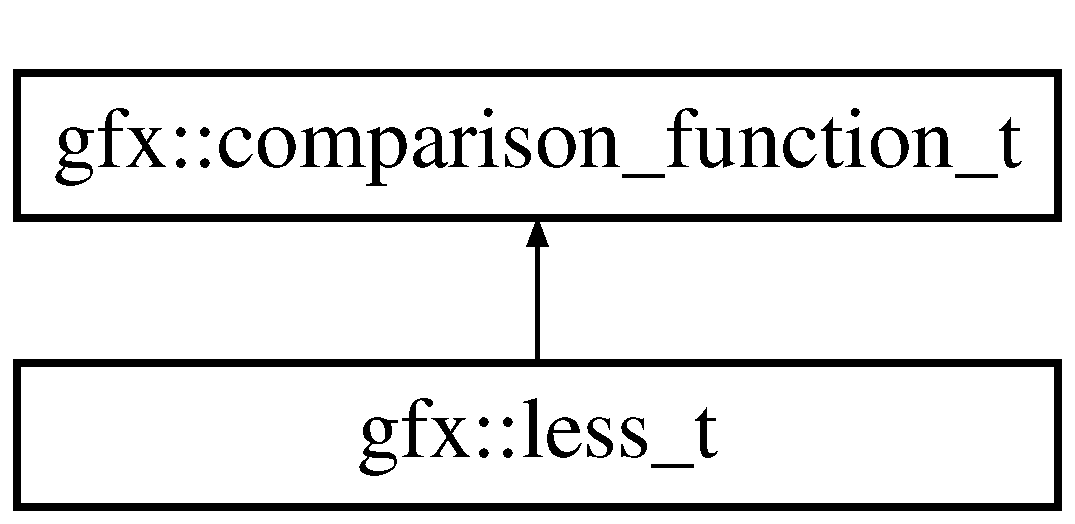
\includegraphics[height=2.000000cm]{classgfx_1_1less__t}
\end{center}
\end{figure}
\subsection*{Protected Member Functions}
\begin{DoxyCompactItemize}
\item 
\hypertarget{classgfx_1_1less__t_ade715f9339c3c788bfb79169abb4d83d}{virtual G\-Lint {\bfseries val} () const }\label{classgfx_1_1less__t_ade715f9339c3c788bfb79169abb4d83d}

\end{DoxyCompactItemize}
\subsection*{Friends}
\begin{DoxyCompactItemize}
\item 
\hypertarget{classgfx_1_1less__t_a2039d67f6166ccf823c78e3476aad9aa}{class {\bfseries texture\-\_\-1\-D}}\label{classgfx_1_1less__t_a2039d67f6166ccf823c78e3476aad9aa}

\item 
\hypertarget{classgfx_1_1less__t_a22ad86ef46c3b17357a0cd59e50bc7dd}{class {\bfseries texture\-\_\-2\-D}}\label{classgfx_1_1less__t_a22ad86ef46c3b17357a0cd59e50bc7dd}

\end{DoxyCompactItemize}


\subsection{Detailed Description}
Selector for the less than comparison function. 

The documentation for this class was generated from the following file\-:\begin{DoxyCompactItemize}
\item 
g\-Scene/texture.\-hpp\end{DoxyCompactItemize}

\hypertarget{classgfx_1_1light}{\section{gfx\-:\-:light Class Reference}
\label{classgfx_1_1light}\index{gfx\-::light@{gfx\-::light}}
}


A representation of a simple light.  




{\ttfamily \#include \char`\"{}g\-Core/g\-Video/light.\-hpp\char`\"{}}

Inheritance diagram for gfx\-:\-:light\-:\begin{figure}[H]
\begin{center}
\leavevmode
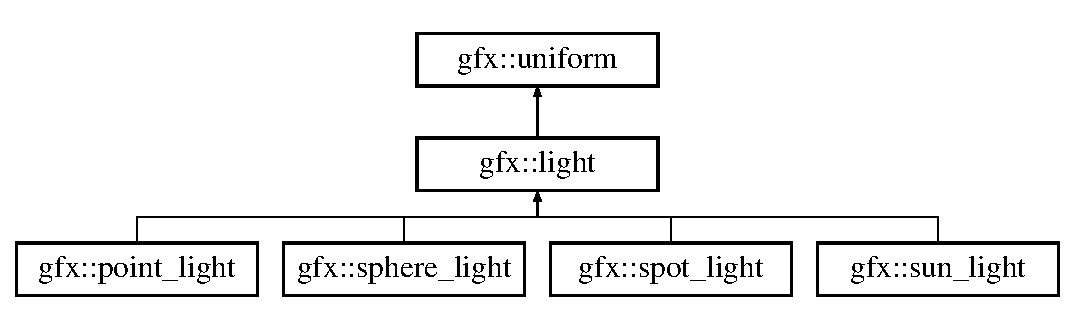
\includegraphics[height=3.000000cm]{classgfx_1_1light}
\end{center}
\end{figure}
\subsection*{Public Member Functions}
\begin{DoxyCompactItemize}
\item 
\hypertarget{classgfx_1_1light_ab6991678227d431b3d022892602d0f60}{\hyperlink{classgfx_1_1light_ab6991678227d431b3d022892602d0f60}{light} ()}\label{classgfx_1_1light_ab6991678227d431b3d022892602d0f60}

\begin{DoxyCompactList}\small\item\em Construct a new light. \end{DoxyCompactList}\item 
virtual void \hyperlink{classgfx_1_1light_a7b974f1340562d8740192b2ff0d62f93}{upload\-\_\-uniform} (\hyperlink{classgfx_1_1program}{program} \&prgm, std\-::string const \&name)
\begin{DoxyCompactList}\small\item\em Upload this light as a uniform to the given \hyperlink{classgfx_1_1program}{program}. \end{DoxyCompactList}\item 
\hyperlink{classgfx_1_1light}{light} \& \hyperlink{classgfx_1_1light_a03e6675928b2d7c1d6ccdf7c18412f41}{radiance} (float rad)
\begin{DoxyCompactList}\small\item\em Set the radiance to the given value. \end{DoxyCompactList}\item 
float \hyperlink{classgfx_1_1light_afb6bafddd687f9ca3b46e40143a4eeb0}{radiance} () const 
\begin{DoxyCompactList}\small\item\em Return the light object's radiance. \end{DoxyCompactList}\end{DoxyCompactItemize}
\subsection*{Protected Attributes}
\begin{DoxyCompactItemize}
\item 
\hypertarget{classgfx_1_1light_afdb046856364ffd67903368add590899}{float {\bfseries rad}}\label{classgfx_1_1light_afdb046856364ffd67903368add590899}

\end{DoxyCompactItemize}
\subsection*{Additional Inherited Members}


\subsection{Detailed Description}
A representation of a simple light. 

Intended as a base class for other lights as this one is missing important rendering information like position or direction. 

\subsection{Member Function Documentation}
\hypertarget{classgfx_1_1light_a03e6675928b2d7c1d6ccdf7c18412f41}{\index{gfx\-::light@{gfx\-::light}!radiance@{radiance}}
\index{radiance@{radiance}!gfx::light@{gfx\-::light}}
\subsubsection[{radiance}]{\setlength{\rightskip}{0pt plus 5cm}{\bf light} \& gfx\-::light\-::radiance (
\begin{DoxyParamCaption}
\item[{float}]{rad}
\end{DoxyParamCaption}
)}}\label{classgfx_1_1light_a03e6675928b2d7c1d6ccdf7c18412f41}


Set the radiance to the given value. 


\begin{DoxyParams}{Parameters}
{\em rad} & The radiance for the light \\
\hline
\end{DoxyParams}
\begin{DoxyReturn}{Returns}
This light object 
\end{DoxyReturn}
\hypertarget{classgfx_1_1light_afb6bafddd687f9ca3b46e40143a4eeb0}{\index{gfx\-::light@{gfx\-::light}!radiance@{radiance}}
\index{radiance@{radiance}!gfx::light@{gfx\-::light}}
\subsubsection[{radiance}]{\setlength{\rightskip}{0pt plus 5cm}float gfx\-::light\-::radiance (
\begin{DoxyParamCaption}
{}
\end{DoxyParamCaption}
) const}}\label{classgfx_1_1light_afb6bafddd687f9ca3b46e40143a4eeb0}


Return the light object's radiance. 

\begin{DoxyReturn}{Returns}
The radiance of the light object. 
\end{DoxyReturn}
\hypertarget{classgfx_1_1light_a7b974f1340562d8740192b2ff0d62f93}{\index{gfx\-::light@{gfx\-::light}!upload\-\_\-uniform@{upload\-\_\-uniform}}
\index{upload\-\_\-uniform@{upload\-\_\-uniform}!gfx::light@{gfx\-::light}}
\subsubsection[{upload\-\_\-uniform}]{\setlength{\rightskip}{0pt plus 5cm}void gfx\-::light\-::upload\-\_\-uniform (
\begin{DoxyParamCaption}
\item[{{\bf program} \&}]{prgm, }
\item[{std\-::string const \&}]{name}
\end{DoxyParamCaption}
)\hspace{0.3cm}{\ttfamily [virtual]}}}\label{classgfx_1_1light_a7b974f1340562d8740192b2ff0d62f93}


Upload this light as a uniform to the given \hyperlink{classgfx_1_1program}{program}. 

\begin{DoxyRefDesc}{Todo}
\item[\hyperlink{todo__todo000019}{Todo}]The uniform class and programs aren't smart enough, yet, for this to work properly. Some shenanigans using an updated info and type system is needed. \end{DoxyRefDesc}


Implements \hyperlink{classgfx_1_1uniform}{gfx\-::uniform}.



Reimplemented in \hyperlink{classgfx_1_1sun__light_a786c5ed1b4b222b38143e7d521459236}{gfx\-::sun\-\_\-light}, \hyperlink{classgfx_1_1spot__light_adde12a9e73e9f00044894af91008c869}{gfx\-::spot\-\_\-light}, \hyperlink{classgfx_1_1sphere__light_a357d9e69656557f7055bfbe6e6952498}{gfx\-::sphere\-\_\-light}, and \hyperlink{classgfx_1_1point__light_a9549403e263927018c000f857cb1e718}{gfx\-::point\-\_\-light}.



The documentation for this class was generated from the following files\-:\begin{DoxyCompactItemize}
\item 
g\-Scene/light.\-hpp\item 
g\-Scene/light.\-cpp\end{DoxyCompactItemize}

\hypertarget{classgfx_1_1linear__mipmap__nearest__t}{\section{gfx\-:\-:linear\-\_\-mipmap\-\_\-nearest\-\_\-t Class Reference}
\label{classgfx_1_1linear__mipmap__nearest__t}\index{gfx\-::linear\-\_\-mipmap\-\_\-nearest\-\_\-t@{gfx\-::linear\-\_\-mipmap\-\_\-nearest\-\_\-t}}
}


Selector for linear image and nearest mipmap filtering.  




{\ttfamily \#include \char`\"{}g\-Core/g\-Video/texture.\-hpp\char`\"{}}

Inheritance diagram for gfx\-:\-:linear\-\_\-mipmap\-\_\-nearest\-\_\-t\-:\begin{figure}[H]
\begin{center}
\leavevmode
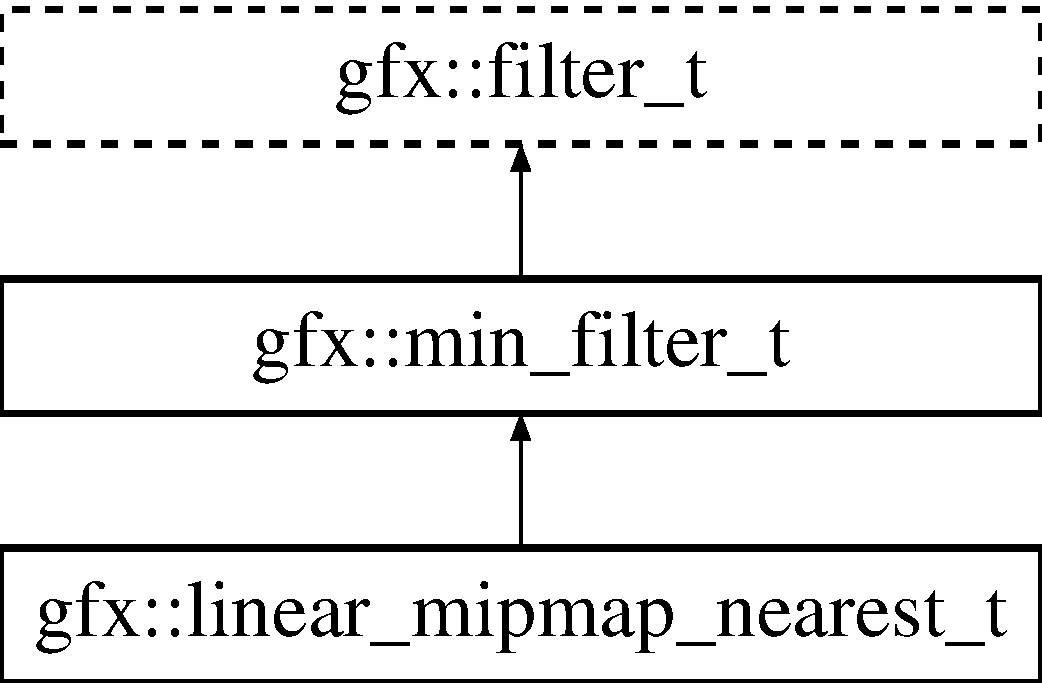
\includegraphics[height=3.000000cm]{classgfx_1_1linear__mipmap__nearest__t}
\end{center}
\end{figure}
\subsection*{Protected Member Functions}
\begin{DoxyCompactItemize}
\item 
\hypertarget{classgfx_1_1linear__mipmap__nearest__t_afce5d8133a2414670f021885d0c809e8}{virtual G\-Lint {\bfseries val} () const }\label{classgfx_1_1linear__mipmap__nearest__t_afce5d8133a2414670f021885d0c809e8}

\end{DoxyCompactItemize}
\subsection*{Friends}
\begin{DoxyCompactItemize}
\item 
\hypertarget{classgfx_1_1linear__mipmap__nearest__t_a2039d67f6166ccf823c78e3476aad9aa}{class {\bfseries texture\-\_\-1\-D}}\label{classgfx_1_1linear__mipmap__nearest__t_a2039d67f6166ccf823c78e3476aad9aa}

\item 
\hypertarget{classgfx_1_1linear__mipmap__nearest__t_a22ad86ef46c3b17357a0cd59e50bc7dd}{class {\bfseries texture\-\_\-2\-D}}\label{classgfx_1_1linear__mipmap__nearest__t_a22ad86ef46c3b17357a0cd59e50bc7dd}

\end{DoxyCompactItemize}


\subsection{Detailed Description}
Selector for linear image and nearest mipmap filtering. 

The documentation for this class was generated from the following file\-:\begin{DoxyCompactItemize}
\item 
g\-Scene/texture.\-hpp\end{DoxyCompactItemize}

\hypertarget{classgfx_1_1linear__mipmap__t}{\section{gfx\-:\-:linear\-\_\-mipmap\-\_\-t Class Reference}
\label{classgfx_1_1linear__mipmap__t}\index{gfx\-::linear\-\_\-mipmap\-\_\-t@{gfx\-::linear\-\_\-mipmap\-\_\-t}}
}


Selector for linear image filtering and mipmapping.  




{\ttfamily \#include \char`\"{}g\-Core/g\-Video/texture.\-hpp\char`\"{}}

Inheritance diagram for gfx\-:\-:linear\-\_\-mipmap\-\_\-t\-:\begin{figure}[H]
\begin{center}
\leavevmode
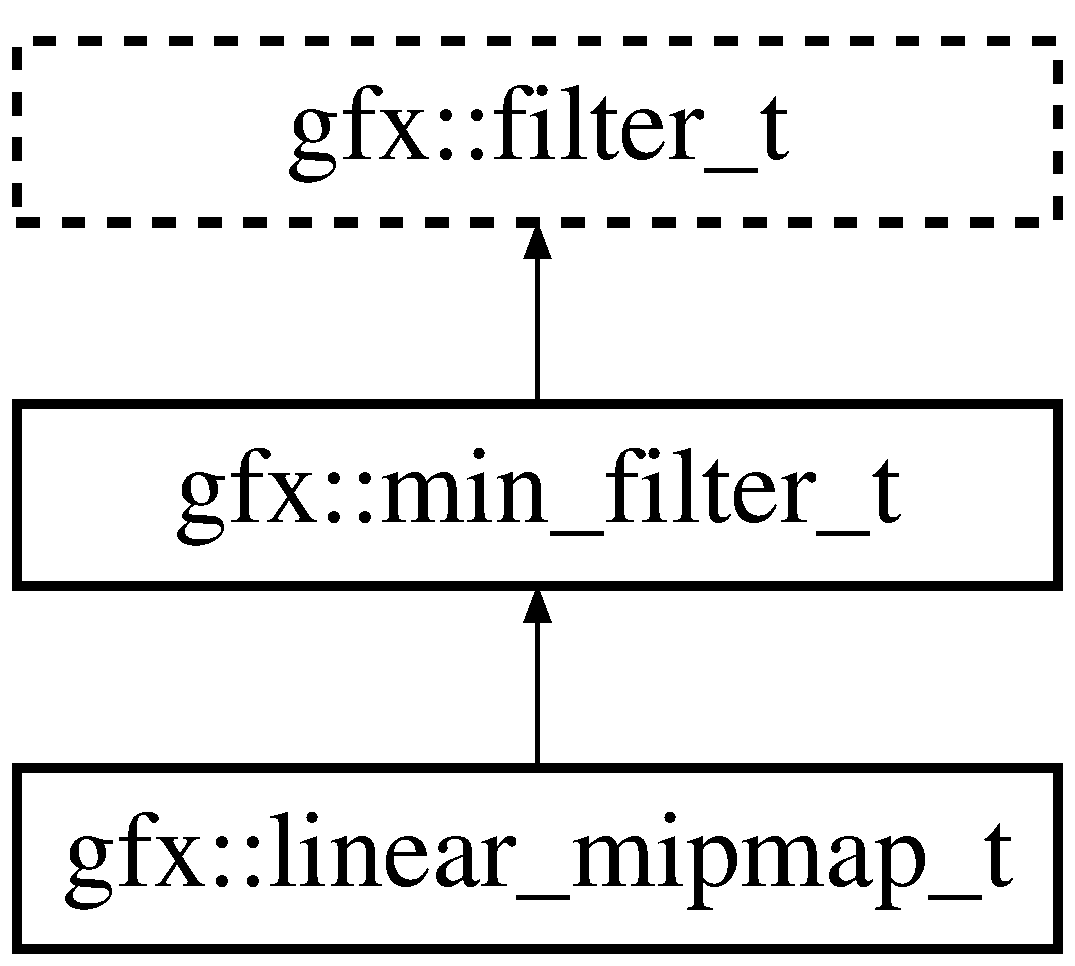
\includegraphics[height=3.000000cm]{classgfx_1_1linear__mipmap__t}
\end{center}
\end{figure}
\subsection*{Protected Member Functions}
\begin{DoxyCompactItemize}
\item 
\hypertarget{classgfx_1_1linear__mipmap__t_aeb5660ee2b7437160621b972f5886f31}{virtual G\-Lint {\bfseries val} () const }\label{classgfx_1_1linear__mipmap__t_aeb5660ee2b7437160621b972f5886f31}

\end{DoxyCompactItemize}
\subsection*{Friends}
\begin{DoxyCompactItemize}
\item 
\hypertarget{classgfx_1_1linear__mipmap__t_a2039d67f6166ccf823c78e3476aad9aa}{class {\bfseries texture\-\_\-1\-D}}\label{classgfx_1_1linear__mipmap__t_a2039d67f6166ccf823c78e3476aad9aa}

\item 
\hypertarget{classgfx_1_1linear__mipmap__t_a22ad86ef46c3b17357a0cd59e50bc7dd}{class {\bfseries texture\-\_\-2\-D}}\label{classgfx_1_1linear__mipmap__t_a22ad86ef46c3b17357a0cd59e50bc7dd}

\end{DoxyCompactItemize}


\subsection{Detailed Description}
Selector for linear image filtering and mipmapping. 

The documentation for this class was generated from the following file\-:\begin{DoxyCompactItemize}
\item 
g\-Scene/texture.\-hpp\end{DoxyCompactItemize}

\hypertarget{classgfx_1_1linear__t}{\section{gfx\-:\-:linear\-\_\-t Class Reference}
\label{classgfx_1_1linear__t}\index{gfx\-::linear\-\_\-t@{gfx\-::linear\-\_\-t}}
}


Selector for linear filtering.  




{\ttfamily \#include \char`\"{}g\-Core/g\-Video/texture.\-hpp\char`\"{}}

Inheritance diagram for gfx\-:\-:linear\-\_\-t\-:\begin{figure}[H]
\begin{center}
\leavevmode
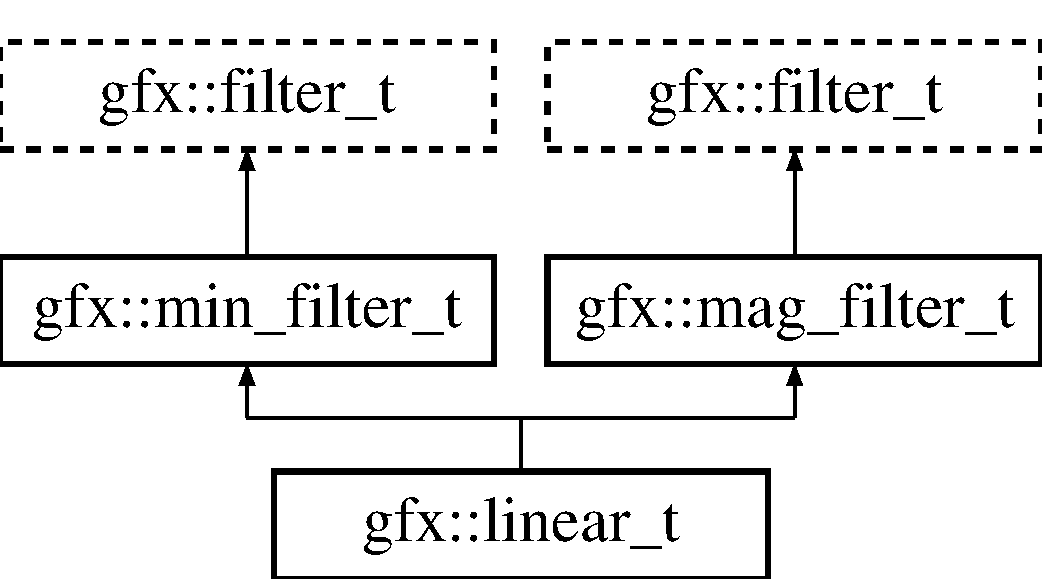
\includegraphics[height=3.000000cm]{classgfx_1_1linear__t}
\end{center}
\end{figure}
\subsection*{Protected Member Functions}
\begin{DoxyCompactItemize}
\item 
\hypertarget{classgfx_1_1linear__t_ab9aa2432c42932752d0f0d9579e17276}{virtual G\-Lint {\bfseries val} () const }\label{classgfx_1_1linear__t_ab9aa2432c42932752d0f0d9579e17276}

\end{DoxyCompactItemize}
\subsection*{Friends}
\begin{DoxyCompactItemize}
\item 
\hypertarget{classgfx_1_1linear__t_a2039d67f6166ccf823c78e3476aad9aa}{class {\bfseries texture\-\_\-1\-D}}\label{classgfx_1_1linear__t_a2039d67f6166ccf823c78e3476aad9aa}

\item 
\hypertarget{classgfx_1_1linear__t_a22ad86ef46c3b17357a0cd59e50bc7dd}{class {\bfseries texture\-\_\-2\-D}}\label{classgfx_1_1linear__t_a22ad86ef46c3b17357a0cd59e50bc7dd}

\end{DoxyCompactItemize}


\subsection{Detailed Description}
Selector for linear filtering. 

The documentation for this class was generated from the following file\-:\begin{DoxyCompactItemize}
\item 
g\-Scene/texture.\-hpp\end{DoxyCompactItemize}

\hypertarget{classgfx_1_1mag__filter__t}{\section{gfx\-:\-:mag\-\_\-filter\-\_\-t Class Reference}
\label{classgfx_1_1mag__filter__t}\index{gfx\-::mag\-\_\-filter\-\_\-t@{gfx\-::mag\-\_\-filter\-\_\-t}}
}


Selector for magnification filtering.  




{\ttfamily \#include \char`\"{}g\-Core/g\-Video/texture.\-hpp\char`\"{}}

Inheritance diagram for gfx\-:\-:mag\-\_\-filter\-\_\-t\-:\begin{figure}[H]
\begin{center}
\leavevmode
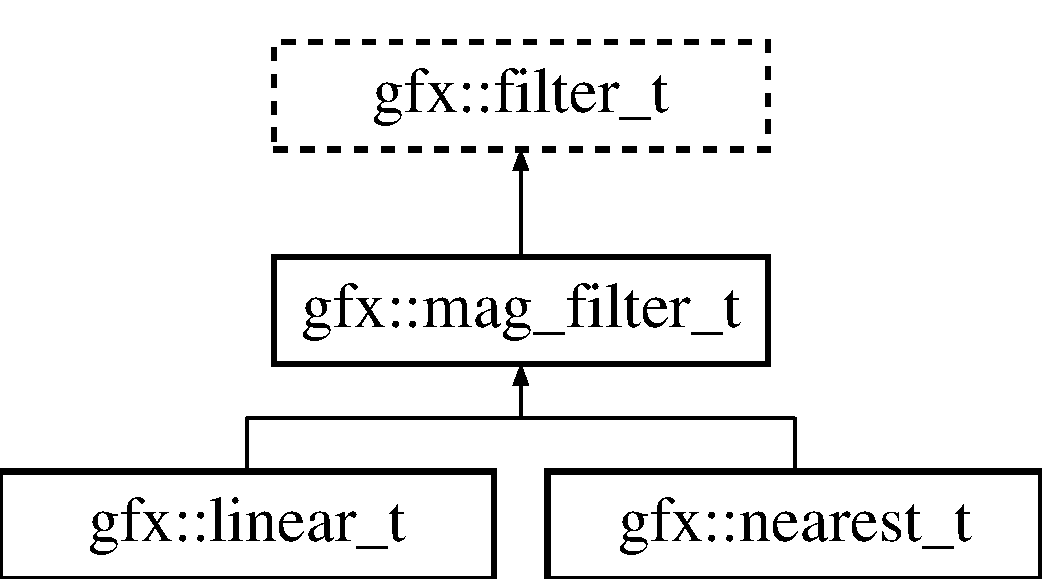
\includegraphics[height=3.000000cm]{classgfx_1_1mag__filter__t}
\end{center}
\end{figure}
\subsection*{Protected Member Functions}
\begin{DoxyCompactItemize}
\item 
\hypertarget{classgfx_1_1mag__filter__t_a3dd85152c225206ec2c6b8c141c1428d}{virtual G\-Lint {\bfseries val} () const =0}\label{classgfx_1_1mag__filter__t_a3dd85152c225206ec2c6b8c141c1428d}

\end{DoxyCompactItemize}
\subsection*{Friends}
\begin{DoxyCompactItemize}
\item 
\hypertarget{classgfx_1_1mag__filter__t_a2039d67f6166ccf823c78e3476aad9aa}{class {\bfseries texture\-\_\-1\-D}}\label{classgfx_1_1mag__filter__t_a2039d67f6166ccf823c78e3476aad9aa}

\item 
\hypertarget{classgfx_1_1mag__filter__t_a22ad86ef46c3b17357a0cd59e50bc7dd}{class {\bfseries texture\-\_\-2\-D}}\label{classgfx_1_1mag__filter__t_a22ad86ef46c3b17357a0cd59e50bc7dd}

\end{DoxyCompactItemize}


\subsection{Detailed Description}
Selector for magnification filtering. 

The documentation for this class was generated from the following file\-:\begin{DoxyCompactItemize}
\item 
g\-Scene/texture.\-hpp\end{DoxyCompactItemize}

\hypertarget{classgfx_1_1min__filter__t}{\section{gfx\-:\-:min\-\_\-filter\-\_\-t Class Reference}
\label{classgfx_1_1min__filter__t}\index{gfx\-::min\-\_\-filter\-\_\-t@{gfx\-::min\-\_\-filter\-\_\-t}}
}


Selector for minification filtering.  




{\ttfamily \#include \char`\"{}g\-Core/g\-Video/texture.\-hpp\char`\"{}}

Inheritance diagram for gfx\-:\-:min\-\_\-filter\-\_\-t\-:\begin{figure}[H]
\begin{center}
\leavevmode
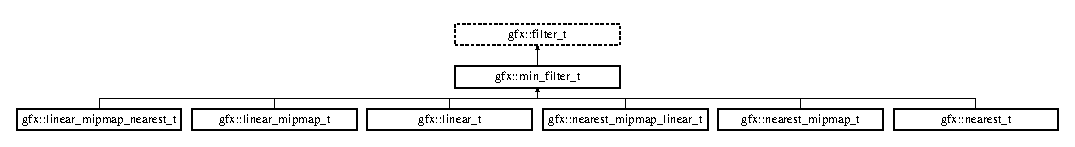
\includegraphics[height=1.530055cm]{classgfx_1_1min__filter__t}
\end{center}
\end{figure}
\subsection*{Protected Member Functions}
\begin{DoxyCompactItemize}
\item 
\hypertarget{classgfx_1_1min__filter__t_a75592c379c8d1a09f9d974967afc6584}{virtual G\-Lint {\bfseries val} () const =0}\label{classgfx_1_1min__filter__t_a75592c379c8d1a09f9d974967afc6584}

\end{DoxyCompactItemize}
\subsection*{Friends}
\begin{DoxyCompactItemize}
\item 
\hypertarget{classgfx_1_1min__filter__t_a2039d67f6166ccf823c78e3476aad9aa}{class {\bfseries texture\-\_\-1\-D}}\label{classgfx_1_1min__filter__t_a2039d67f6166ccf823c78e3476aad9aa}

\item 
\hypertarget{classgfx_1_1min__filter__t_a22ad86ef46c3b17357a0cd59e50bc7dd}{class {\bfseries texture\-\_\-2\-D}}\label{classgfx_1_1min__filter__t_a22ad86ef46c3b17357a0cd59e50bc7dd}

\end{DoxyCompactItemize}


\subsection{Detailed Description}
Selector for minification filtering. 

The documentation for this class was generated from the following file\-:\begin{DoxyCompactItemize}
\item 
g\-Scene/texture.\-hpp\end{DoxyCompactItemize}

\hypertarget{classgfx_1_1mirrored__repeat__t}{\section{gfx\-:\-:mirrored\-\_\-repeat\-\_\-t Class Reference}
\label{classgfx_1_1mirrored__repeat__t}\index{gfx\-::mirrored\-\_\-repeat\-\_\-t@{gfx\-::mirrored\-\_\-repeat\-\_\-t}}
}


Selector for mirrored repeat sampling.  




{\ttfamily \#include \char`\"{}g\-Core/g\-Video/texture.\-hpp\char`\"{}}

Inheritance diagram for gfx\-:\-:mirrored\-\_\-repeat\-\_\-t\-:\begin{figure}[H]
\begin{center}
\leavevmode
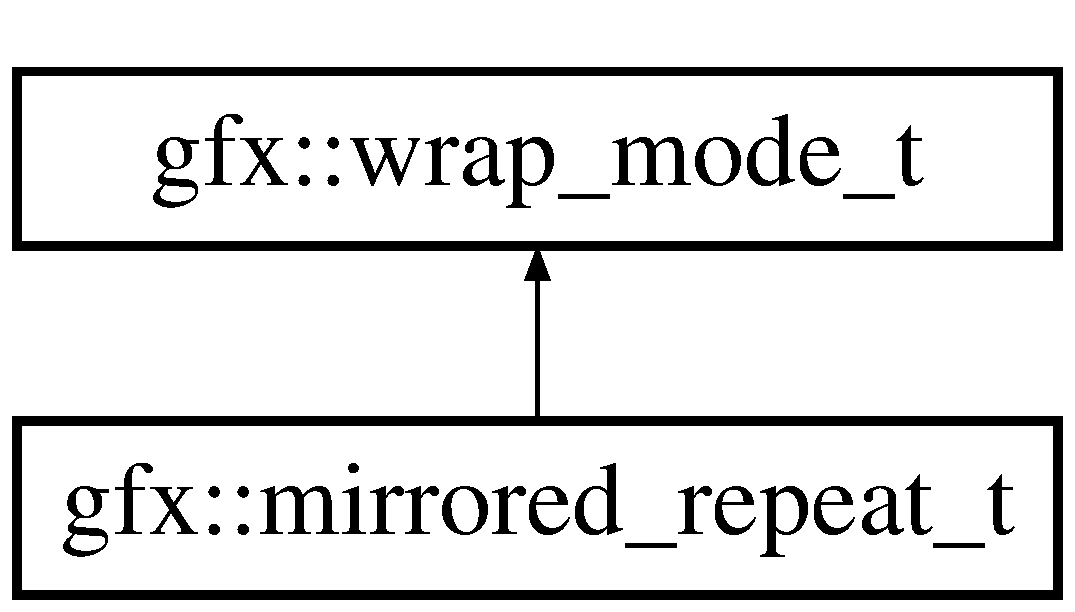
\includegraphics[height=2.000000cm]{classgfx_1_1mirrored__repeat__t}
\end{center}
\end{figure}
\subsection*{Protected Member Functions}
\begin{DoxyCompactItemize}
\item 
\hypertarget{classgfx_1_1mirrored__repeat__t_aa0f1593025076337359fbb9385f4d52b}{virtual G\-Lint {\bfseries val} () const }\label{classgfx_1_1mirrored__repeat__t_aa0f1593025076337359fbb9385f4d52b}

\end{DoxyCompactItemize}
\subsection*{Friends}
\begin{DoxyCompactItemize}
\item 
\hypertarget{classgfx_1_1mirrored__repeat__t_a2039d67f6166ccf823c78e3476aad9aa}{class {\bfseries texture\-\_\-1\-D}}\label{classgfx_1_1mirrored__repeat__t_a2039d67f6166ccf823c78e3476aad9aa}

\item 
\hypertarget{classgfx_1_1mirrored__repeat__t_a22ad86ef46c3b17357a0cd59e50bc7dd}{class {\bfseries texture\-\_\-2\-D}}\label{classgfx_1_1mirrored__repeat__t_a22ad86ef46c3b17357a0cd59e50bc7dd}

\end{DoxyCompactItemize}


\subsection{Detailed Description}
Selector for mirrored repeat sampling. 

The documentation for this class was generated from the following file\-:\begin{DoxyCompactItemize}
\item 
g\-Scene/texture.\-hpp\end{DoxyCompactItemize}

\hypertarget{classgfx_1_1nearest__mipmap__linear__t}{\section{gfx\-:\-:nearest\-\_\-mipmap\-\_\-linear\-\_\-t Class Reference}
\label{classgfx_1_1nearest__mipmap__linear__t}\index{gfx\-::nearest\-\_\-mipmap\-\_\-linear\-\_\-t@{gfx\-::nearest\-\_\-mipmap\-\_\-linear\-\_\-t}}
}


Selector for nearest image and linear mipmap filtering.  




{\ttfamily \#include \char`\"{}g\-Core/g\-Video/texture.\-hpp\char`\"{}}

Inheritance diagram for gfx\-:\-:nearest\-\_\-mipmap\-\_\-linear\-\_\-t\-:\begin{figure}[H]
\begin{center}
\leavevmode
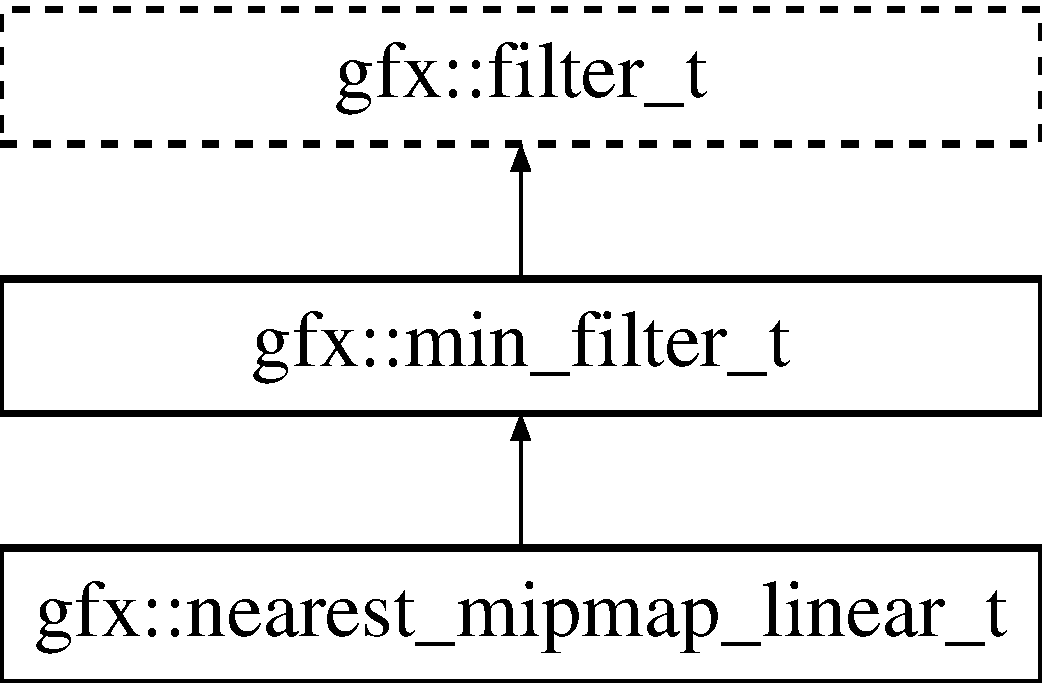
\includegraphics[height=3.000000cm]{classgfx_1_1nearest__mipmap__linear__t}
\end{center}
\end{figure}
\subsection*{Protected Member Functions}
\begin{DoxyCompactItemize}
\item 
\hypertarget{classgfx_1_1nearest__mipmap__linear__t_a62bfc0c869597d99ad9e18114d68875c}{virtual G\-Lint {\bfseries val} () const }\label{classgfx_1_1nearest__mipmap__linear__t_a62bfc0c869597d99ad9e18114d68875c}

\end{DoxyCompactItemize}
\subsection*{Friends}
\begin{DoxyCompactItemize}
\item 
\hypertarget{classgfx_1_1nearest__mipmap__linear__t_a2039d67f6166ccf823c78e3476aad9aa}{class {\bfseries texture\-\_\-1\-D}}\label{classgfx_1_1nearest__mipmap__linear__t_a2039d67f6166ccf823c78e3476aad9aa}

\item 
\hypertarget{classgfx_1_1nearest__mipmap__linear__t_a22ad86ef46c3b17357a0cd59e50bc7dd}{class {\bfseries texture\-\_\-2\-D}}\label{classgfx_1_1nearest__mipmap__linear__t_a22ad86ef46c3b17357a0cd59e50bc7dd}

\end{DoxyCompactItemize}


\subsection{Detailed Description}
Selector for nearest image and linear mipmap filtering. 

The documentation for this class was generated from the following file\-:\begin{DoxyCompactItemize}
\item 
g\-Scene/texture.\-hpp\end{DoxyCompactItemize}

\hypertarget{classgfx_1_1nearest__mipmap__t}{\section{gfx\-:\-:nearest\-\_\-mipmap\-\_\-t Class Reference}
\label{classgfx_1_1nearest__mipmap__t}\index{gfx\-::nearest\-\_\-mipmap\-\_\-t@{gfx\-::nearest\-\_\-mipmap\-\_\-t}}
}


Selector for nearest mipmap filtering.  




{\ttfamily \#include \char`\"{}g\-Core/g\-Video/texture.\-hpp\char`\"{}}

Inheritance diagram for gfx\-:\-:nearest\-\_\-mipmap\-\_\-t\-:\begin{figure}[H]
\begin{center}
\leavevmode
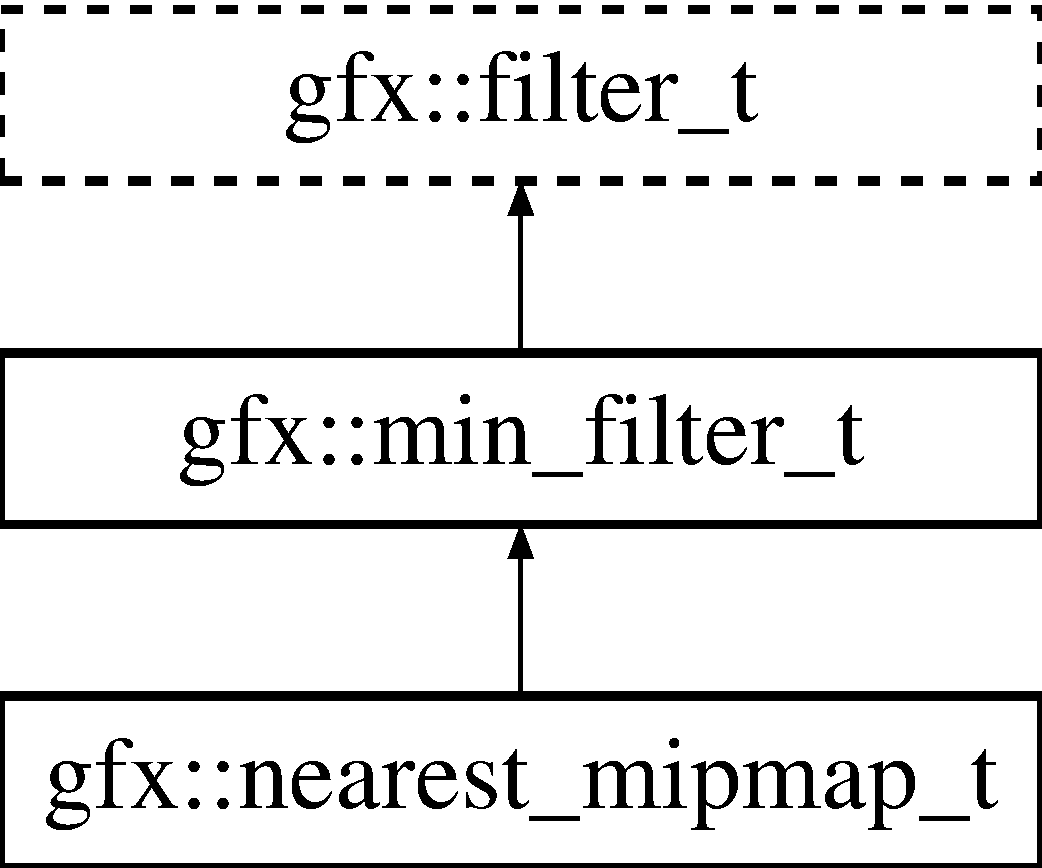
\includegraphics[height=3.000000cm]{classgfx_1_1nearest__mipmap__t}
\end{center}
\end{figure}
\subsection*{Protected Member Functions}
\begin{DoxyCompactItemize}
\item 
\hypertarget{classgfx_1_1nearest__mipmap__t_ac1bf4967d54ebe3b79956869529fe942}{virtual G\-Lint {\bfseries val} () const }\label{classgfx_1_1nearest__mipmap__t_ac1bf4967d54ebe3b79956869529fe942}

\end{DoxyCompactItemize}
\subsection*{Friends}
\begin{DoxyCompactItemize}
\item 
\hypertarget{classgfx_1_1nearest__mipmap__t_a2039d67f6166ccf823c78e3476aad9aa}{class {\bfseries texture\-\_\-1\-D}}\label{classgfx_1_1nearest__mipmap__t_a2039d67f6166ccf823c78e3476aad9aa}

\item 
\hypertarget{classgfx_1_1nearest__mipmap__t_a22ad86ef46c3b17357a0cd59e50bc7dd}{class {\bfseries texture\-\_\-2\-D}}\label{classgfx_1_1nearest__mipmap__t_a22ad86ef46c3b17357a0cd59e50bc7dd}

\end{DoxyCompactItemize}


\subsection{Detailed Description}
Selector for nearest mipmap filtering. 

The documentation for this class was generated from the following file\-:\begin{DoxyCompactItemize}
\item 
g\-Scene/texture.\-hpp\end{DoxyCompactItemize}

\hypertarget{classgfx_1_1nearest__t}{\section{gfx\-:\-:nearest\-\_\-t Class Reference}
\label{classgfx_1_1nearest__t}\index{gfx\-::nearest\-\_\-t@{gfx\-::nearest\-\_\-t}}
}


Selector for nearest filtering.  




{\ttfamily \#include \char`\"{}g\-Core/g\-Video/texture.\-hpp\char`\"{}}

Inheritance diagram for gfx\-:\-:nearest\-\_\-t\-:\begin{figure}[H]
\begin{center}
\leavevmode
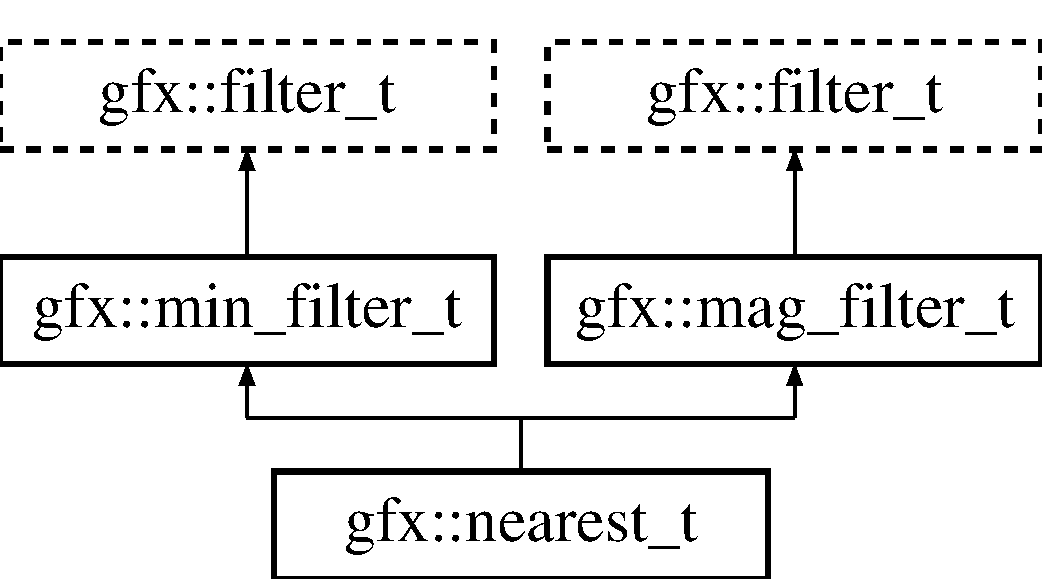
\includegraphics[height=3.000000cm]{classgfx_1_1nearest__t}
\end{center}
\end{figure}
\subsection*{Protected Member Functions}
\begin{DoxyCompactItemize}
\item 
\hypertarget{classgfx_1_1nearest__t_ad8696065b222f006a37aebbc626455bf}{virtual G\-Lint {\bfseries val} () const }\label{classgfx_1_1nearest__t_ad8696065b222f006a37aebbc626455bf}

\end{DoxyCompactItemize}
\subsection*{Friends}
\begin{DoxyCompactItemize}
\item 
\hypertarget{classgfx_1_1nearest__t_a2039d67f6166ccf823c78e3476aad9aa}{class {\bfseries texture\-\_\-1\-D}}\label{classgfx_1_1nearest__t_a2039d67f6166ccf823c78e3476aad9aa}

\item 
\hypertarget{classgfx_1_1nearest__t_a22ad86ef46c3b17357a0cd59e50bc7dd}{class {\bfseries texture\-\_\-2\-D}}\label{classgfx_1_1nearest__t_a22ad86ef46c3b17357a0cd59e50bc7dd}

\end{DoxyCompactItemize}


\subsection{Detailed Description}
Selector for nearest filtering. 

The documentation for this class was generated from the following file\-:\begin{DoxyCompactItemize}
\item 
g\-Scene/texture.\-hpp\end{DoxyCompactItemize}

\hypertarget{classgfx_1_1never__t}{\section{gfx\-:\-:never\-\_\-t Class Reference}
\label{classgfx_1_1never__t}\index{gfx\-::never\-\_\-t@{gfx\-::never\-\_\-t}}
}


Selector for the never comparison function.  




{\ttfamily \#include \char`\"{}g\-Core/g\-Video/texture.\-hpp\char`\"{}}

Inheritance diagram for gfx\-:\-:never\-\_\-t\-:\begin{figure}[H]
\begin{center}
\leavevmode
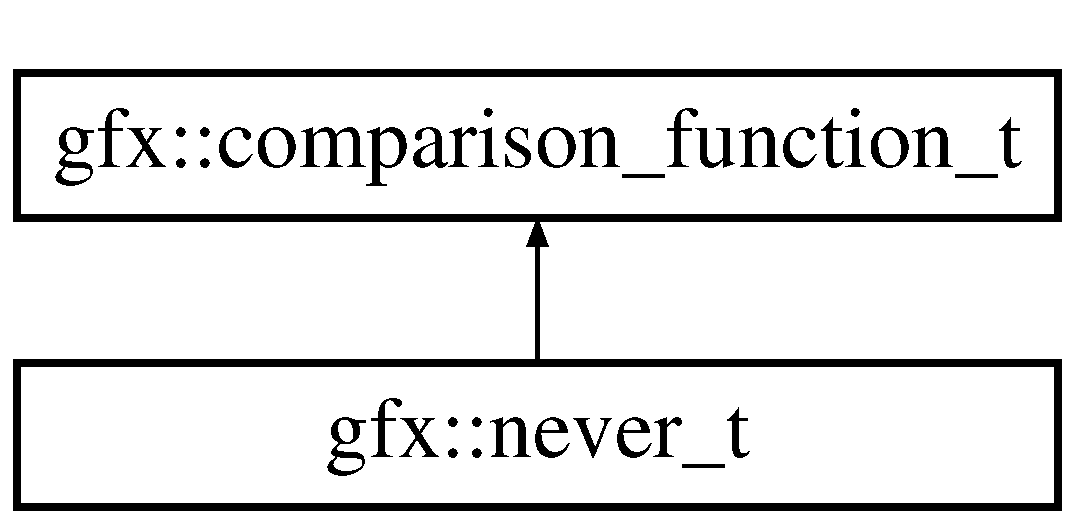
\includegraphics[height=2.000000cm]{classgfx_1_1never__t}
\end{center}
\end{figure}
\subsection*{Protected Member Functions}
\begin{DoxyCompactItemize}
\item 
\hypertarget{classgfx_1_1never__t_ab27939641421e1bfa55ae66314cad817}{virtual G\-Lint {\bfseries val} () const }\label{classgfx_1_1never__t_ab27939641421e1bfa55ae66314cad817}

\end{DoxyCompactItemize}
\subsection*{Friends}
\begin{DoxyCompactItemize}
\item 
\hypertarget{classgfx_1_1never__t_a2039d67f6166ccf823c78e3476aad9aa}{class {\bfseries texture\-\_\-1\-D}}\label{classgfx_1_1never__t_a2039d67f6166ccf823c78e3476aad9aa}

\item 
\hypertarget{classgfx_1_1never__t_a22ad86ef46c3b17357a0cd59e50bc7dd}{class {\bfseries texture\-\_\-2\-D}}\label{classgfx_1_1never__t_a22ad86ef46c3b17357a0cd59e50bc7dd}

\end{DoxyCompactItemize}


\subsection{Detailed Description}
Selector for the never comparison function. 

The documentation for this class was generated from the following file\-:\begin{DoxyCompactItemize}
\item 
g\-Scene/texture.\-hpp\end{DoxyCompactItemize}

\hypertarget{classgfx_1_1not__equal__t}{\section{gfx\-:\-:not\-\_\-equal\-\_\-t Class Reference}
\label{classgfx_1_1not__equal__t}\index{gfx\-::not\-\_\-equal\-\_\-t@{gfx\-::not\-\_\-equal\-\_\-t}}
}


Selector for the not equal to comparison function.  




{\ttfamily \#include \char`\"{}g\-Core/g\-Video/texture.\-hpp\char`\"{}}

Inheritance diagram for gfx\-:\-:not\-\_\-equal\-\_\-t\-:\begin{figure}[H]
\begin{center}
\leavevmode
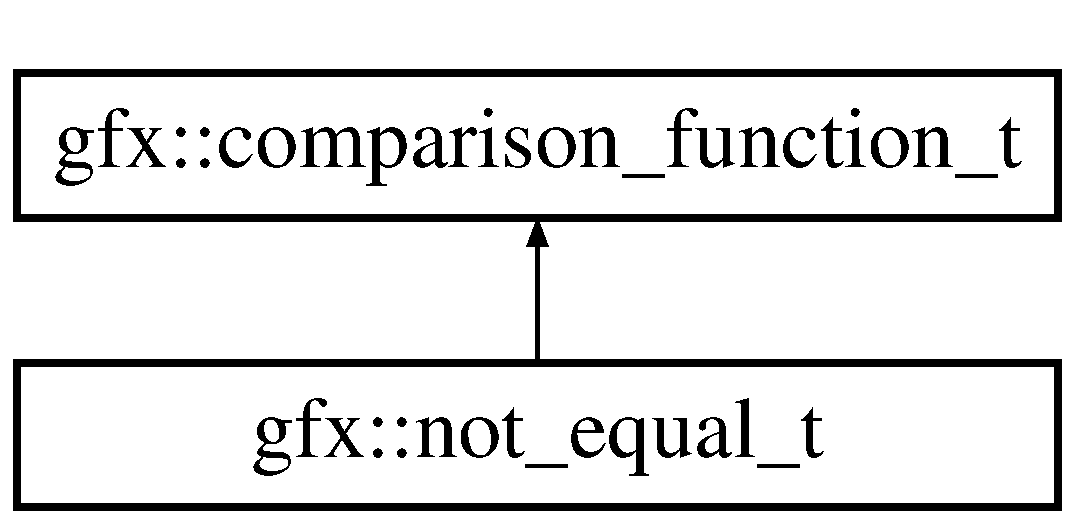
\includegraphics[height=2.000000cm]{classgfx_1_1not__equal__t}
\end{center}
\end{figure}
\subsection*{Protected Member Functions}
\begin{DoxyCompactItemize}
\item 
\hypertarget{classgfx_1_1not__equal__t_acb3d2a78c702618c29e26cbab8d94a31}{virtual G\-Lint {\bfseries val} () const }\label{classgfx_1_1not__equal__t_acb3d2a78c702618c29e26cbab8d94a31}

\end{DoxyCompactItemize}
\subsection*{Friends}
\begin{DoxyCompactItemize}
\item 
\hypertarget{classgfx_1_1not__equal__t_a2039d67f6166ccf823c78e3476aad9aa}{class {\bfseries texture\-\_\-1\-D}}\label{classgfx_1_1not__equal__t_a2039d67f6166ccf823c78e3476aad9aa}

\item 
\hypertarget{classgfx_1_1not__equal__t_a22ad86ef46c3b17357a0cd59e50bc7dd}{class {\bfseries texture\-\_\-2\-D}}\label{classgfx_1_1not__equal__t_a22ad86ef46c3b17357a0cd59e50bc7dd}

\end{DoxyCompactItemize}


\subsection{Detailed Description}
Selector for the not equal to comparison function. 

The documentation for this class was generated from the following file\-:\begin{DoxyCompactItemize}
\item 
g\-Scene/texture.\-hpp\end{DoxyCompactItemize}

\hypertarget{classgfx_1_1orientable}{\section{gfx\-:\-:orientable Class Reference}
\label{classgfx_1_1orientable}\index{gfx\-::orientable@{gfx\-::orientable}}
}


A base class for any object that can be oriented in 3-\/space.  




{\ttfamily \#include \char`\"{}g\-Core/gscne/orientable.\-hpp\char`\"{}}

Inheritance diagram for gfx\-:\-:orientable\-:\begin{figure}[H]
\begin{center}
\leavevmode
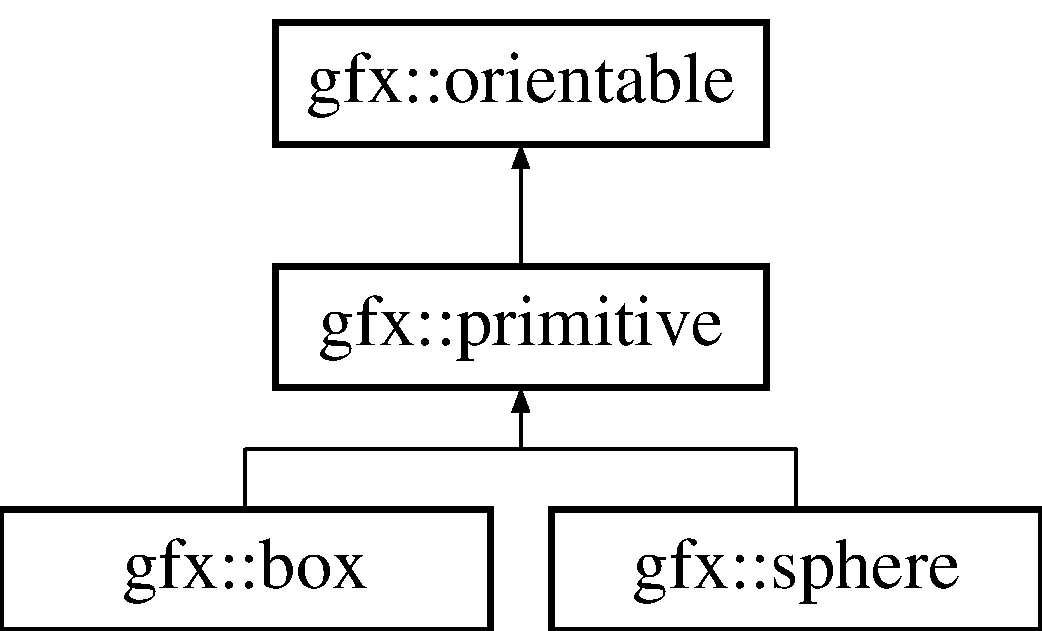
\includegraphics[height=3.000000cm]{classgfx_1_1orientable}
\end{center}
\end{figure}
\subsection*{Classes}
\begin{DoxyCompactItemize}
\item 
class \hyperlink{classgfx_1_1orientable_1_1settings}{settings}
\end{DoxyCompactItemize}
\subsection*{Public Member Functions}
\begin{DoxyCompactItemize}
\item 
\hypertarget{classgfx_1_1orientable_a053f20c5e02879540199c0e232636d0b}{\hyperlink{classgfx_1_1orientable_a053f20c5e02879540199c0e232636d0b}{orientable} (\hyperlink{classgfx_1_1orientable_1_1settings}{settings} const \&set=\hyperlink{classgfx_1_1orientable_1_1settings}{settings}())}\label{classgfx_1_1orientable_a053f20c5e02879540199c0e232636d0b}

\begin{DoxyCompactList}\small\item\em Construct a new orientable object. \end{DoxyCompactList}\item 
\hypertarget{classgfx_1_1orientable_a88fbeffe72a67ff7169ab2aea6109e6c}{\hyperlink{classgfx_1_1orientable}{orientable} \& {\bfseries scale} (vec3 const \&scl)}\label{classgfx_1_1orientable_a88fbeffe72a67ff7169ab2aea6109e6c}

\item 
\hyperlink{classgfx_1_1orientable}{orientable} \& \hyperlink{classgfx_1_1orientable_abbddb58aba9e2b1d2011cc5d8b289e7a}{stretch} (vec3 const \&scl)
\begin{DoxyCompactList}\small\item\em Set the scale of the orientable object. \end{DoxyCompactList}\item 
vec3 const \& \hyperlink{classgfx_1_1orientable_a1a4029fefd371cb0d54b1ba279824223}{scale} () const 
\begin{DoxyCompactList}\small\item\em Return the scale of the orientable object. \end{DoxyCompactList}\item 
\hypertarget{classgfx_1_1orientable_a9b65cffc474e9939879af5cebff5c193}{\hyperlink{classgfx_1_1orientable}{orientable} \& {\bfseries rotation} (qutn const \&rot)}\label{classgfx_1_1orientable_a9b65cffc474e9939879af5cebff5c193}

\item 
\hyperlink{classgfx_1_1orientable}{orientable} \& \hyperlink{classgfx_1_1orientable_a5c66e5f024408cdf71153bfbc444d7f3}{rotate} (qutn const \&rot)
\begin{DoxyCompactList}\small\item\em Set the rotation of the orientable object. \end{DoxyCompactList}\item 
qutn const \& \hyperlink{classgfx_1_1orientable_a8e7131168074ee2d76d83313c883fe76}{rotation} () const 
\begin{DoxyCompactList}\small\item\em Return the rotation of the orientable object. \end{DoxyCompactList}\item 
\hyperlink{classgfx_1_1orientable}{orientable} \& \hyperlink{classgfx_1_1orientable_a34690e36f7c1623db703903b26ef5239}{position} (vec3 const \&pos)
\begin{DoxyCompactList}\small\item\em Return the position of the orientable object. \end{DoxyCompactList}\item 
\hyperlink{classgfx_1_1orientable}{orientable} \& \hyperlink{classgfx_1_1orientable_ac9221e15f972b8c2ba4e530cc8be4535}{move} (vec3 const \&mov)
\begin{DoxyCompactList}\small\item\em Set the position of the orientable object. \end{DoxyCompactList}\item 
vec3 const \& \hyperlink{classgfx_1_1orientable_aae8b96c0c3a5b5f86c622c7687616644}{position} () const 
\begin{DoxyCompactList}\small\item\em Return the position of the orientable object. \end{DoxyCompactList}\item 
mat4 const \& \hyperlink{classgfx_1_1orientable_a775c3fac31386a99802c2d3169ae8481}{object\-\_\-matrix} () const 
\begin{DoxyCompactList}\small\item\em Return the transformation matrix of this orientable object. \end{DoxyCompactList}\end{DoxyCompactItemize}
\subsection*{Protected Member Functions}
\begin{DoxyCompactItemize}
\item 
\hypertarget{classgfx_1_1orientable_ac49e3e938ffb892a8c55e7cb88d8bbe0}{void \hyperlink{classgfx_1_1orientable_ac49e3e938ffb892a8c55e7cb88d8bbe0}{update\-\_\-obj\-\_\-mtrx} ()}\label{classgfx_1_1orientable_ac49e3e938ffb892a8c55e7cb88d8bbe0}

\begin{DoxyCompactList}\small\item\em Generate the trnasformation matrix from current settings. \end{DoxyCompactList}\end{DoxyCompactItemize}
\subsection*{Protected Attributes}
\begin{DoxyCompactItemize}
\item 
\hypertarget{classgfx_1_1orientable_a54e3ccf1da2a2a5fabd7292c60348b1b}{bool {\bfseries orientation\-\_\-changed}}\label{classgfx_1_1orientable_a54e3ccf1da2a2a5fabd7292c60348b1b}

\end{DoxyCompactItemize}


\subsection{Detailed Description}
A base class for any object that can be oriented in 3-\/space. 

The rule with multiple inheritance is usually that you should keep as much implementation out of the base classes in the multiply inherited class tree. This class would ignore that rule is it is used as a base class. I'm leaning towards using the composition pattern from the mobile game, as it worked pretty well there. In that case, orientable would just be another component and not much would have to change (other than inheriting the base component class).

Orientable implicitly means that the object exists within simulation space; orientable objects are N\-O\-T used for any sort of G\-U\-I elements or effects objects which have non-\/euclidean properties (such as a sky box). Orientable does N\-O\-T imply that the object is collidable, though. That would be the job of the (as yet unwritten) collidable class. 

\subsection{Member Function Documentation}
\hypertarget{classgfx_1_1orientable_ac9221e15f972b8c2ba4e530cc8be4535}{\index{gfx\-::orientable@{gfx\-::orientable}!move@{move}}
\index{move@{move}!gfx::orientable@{gfx\-::orientable}}
\subsubsection[{move}]{\setlength{\rightskip}{0pt plus 5cm}{\bf orientable} \& gfx\-::orientable\-::move (
\begin{DoxyParamCaption}
\item[{vec3 const \&}]{mov}
\end{DoxyParamCaption}
)}}\label{classgfx_1_1orientable_ac9221e15f972b8c2ba4e530cc8be4535}


Set the position of the orientable object. 


\begin{DoxyParams}{Parameters}
{\em stc} & The position of the orientable object. \\
\hline
\end{DoxyParams}
\begin{DoxyReturn}{Returns}
This orientable object 
\end{DoxyReturn}
\hypertarget{classgfx_1_1orientable_a775c3fac31386a99802c2d3169ae8481}{\index{gfx\-::orientable@{gfx\-::orientable}!object\-\_\-matrix@{object\-\_\-matrix}}
\index{object\-\_\-matrix@{object\-\_\-matrix}!gfx::orientable@{gfx\-::orientable}}
\subsubsection[{object\-\_\-matrix}]{\setlength{\rightskip}{0pt plus 5cm}mat4 const \& gfx\-::orientable\-::object\-\_\-matrix (
\begin{DoxyParamCaption}
{}
\end{DoxyParamCaption}
) const}}\label{classgfx_1_1orientable_a775c3fac31386a99802c2d3169ae8481}


Return the transformation matrix of this orientable object. 

\begin{DoxyReturn}{Returns}
The transformaton of the orientable object. 
\end{DoxyReturn}
\hypertarget{classgfx_1_1orientable_a34690e36f7c1623db703903b26ef5239}{\index{gfx\-::orientable@{gfx\-::orientable}!position@{position}}
\index{position@{position}!gfx::orientable@{gfx\-::orientable}}
\subsubsection[{position}]{\setlength{\rightskip}{0pt plus 5cm}{\bf orientable} \& gfx\-::orientable\-::position (
\begin{DoxyParamCaption}
\item[{vec3 const \&}]{pos}
\end{DoxyParamCaption}
)}}\label{classgfx_1_1orientable_a34690e36f7c1623db703903b26ef5239}


Return the position of the orientable object. 

\begin{DoxyReturn}{Returns}
The position of the orientable object. 
\end{DoxyReturn}
\hypertarget{classgfx_1_1orientable_aae8b96c0c3a5b5f86c622c7687616644}{\index{gfx\-::orientable@{gfx\-::orientable}!position@{position}}
\index{position@{position}!gfx::orientable@{gfx\-::orientable}}
\subsubsection[{position}]{\setlength{\rightskip}{0pt plus 5cm}vec3 const \& gfx\-::orientable\-::position (
\begin{DoxyParamCaption}
{}
\end{DoxyParamCaption}
) const\hspace{0.3cm}{\ttfamily [inline]}}}\label{classgfx_1_1orientable_aae8b96c0c3a5b5f86c622c7687616644}


Return the position of the orientable object. 

\begin{DoxyReturn}{Returns}
The position of the orientable object. 
\end{DoxyReturn}
\hypertarget{classgfx_1_1orientable_a5c66e5f024408cdf71153bfbc444d7f3}{\index{gfx\-::orientable@{gfx\-::orientable}!rotate@{rotate}}
\index{rotate@{rotate}!gfx::orientable@{gfx\-::orientable}}
\subsubsection[{rotate}]{\setlength{\rightskip}{0pt plus 5cm}{\bf orientable} \& gfx\-::orientable\-::rotate (
\begin{DoxyParamCaption}
\item[{qutn const \&}]{rot}
\end{DoxyParamCaption}
)}}\label{classgfx_1_1orientable_a5c66e5f024408cdf71153bfbc444d7f3}


Set the rotation of the orientable object. 


\begin{DoxyParams}{Parameters}
{\em stc} & The rotation of the orientable object. \\
\hline
\end{DoxyParams}
\begin{DoxyReturn}{Returns}
This orientable object 
\end{DoxyReturn}
\hypertarget{classgfx_1_1orientable_a8e7131168074ee2d76d83313c883fe76}{\index{gfx\-::orientable@{gfx\-::orientable}!rotation@{rotation}}
\index{rotation@{rotation}!gfx::orientable@{gfx\-::orientable}}
\subsubsection[{rotation}]{\setlength{\rightskip}{0pt plus 5cm}qutn const \& gfx\-::orientable\-::rotation (
\begin{DoxyParamCaption}
{}
\end{DoxyParamCaption}
) const\hspace{0.3cm}{\ttfamily [inline]}}}\label{classgfx_1_1orientable_a8e7131168074ee2d76d83313c883fe76}


Return the rotation of the orientable object. 

\begin{DoxyReturn}{Returns}
The rotation of the orientable object. 
\end{DoxyReturn}
\hypertarget{classgfx_1_1orientable_a1a4029fefd371cb0d54b1ba279824223}{\index{gfx\-::orientable@{gfx\-::orientable}!scale@{scale}}
\index{scale@{scale}!gfx::orientable@{gfx\-::orientable}}
\subsubsection[{scale}]{\setlength{\rightskip}{0pt plus 5cm}vec3 const \& gfx\-::orientable\-::scale (
\begin{DoxyParamCaption}
{}
\end{DoxyParamCaption}
) const\hspace{0.3cm}{\ttfamily [inline]}}}\label{classgfx_1_1orientable_a1a4029fefd371cb0d54b1ba279824223}


Return the scale of the orientable object. 

\begin{DoxyReturn}{Returns}
The scale of the orientable object. 
\end{DoxyReturn}
\hypertarget{classgfx_1_1orientable_abbddb58aba9e2b1d2011cc5d8b289e7a}{\index{gfx\-::orientable@{gfx\-::orientable}!stretch@{stretch}}
\index{stretch@{stretch}!gfx::orientable@{gfx\-::orientable}}
\subsubsection[{stretch}]{\setlength{\rightskip}{0pt plus 5cm}{\bf orientable} \& gfx\-::orientable\-::stretch (
\begin{DoxyParamCaption}
\item[{vec3 const \&}]{stc}
\end{DoxyParamCaption}
)}}\label{classgfx_1_1orientable_abbddb58aba9e2b1d2011cc5d8b289e7a}


Set the scale of the orientable object. 


\begin{DoxyParams}{Parameters}
{\em stc} & The scale of the orientable object. \\
\hline
\end{DoxyParams}
\begin{DoxyReturn}{Returns}
This orientable object 
\end{DoxyReturn}


The documentation for this class was generated from the following files\-:\begin{DoxyCompactItemize}
\item 
g\-Scene/orientable.\-hpp\item 
g\-Scene/orientable.\-cpp\end{DoxyCompactItemize}

\hypertarget{classgfx_1_1ortho__cam}{\section{gfx\-:\-:ortho\-\_\-cam Class Reference}
\label{classgfx_1_1ortho__cam}\index{gfx\-::ortho\-\_\-cam@{gfx\-::ortho\-\_\-cam}}
}


An orthographic camera.  




{\ttfamily \#include \char`\"{}g\-Core/g\-Scene/camera/hpp\char`\"{}}

Inheritance diagram for gfx\-:\-:ortho\-\_\-cam\-:\begin{figure}[H]
\begin{center}
\leavevmode
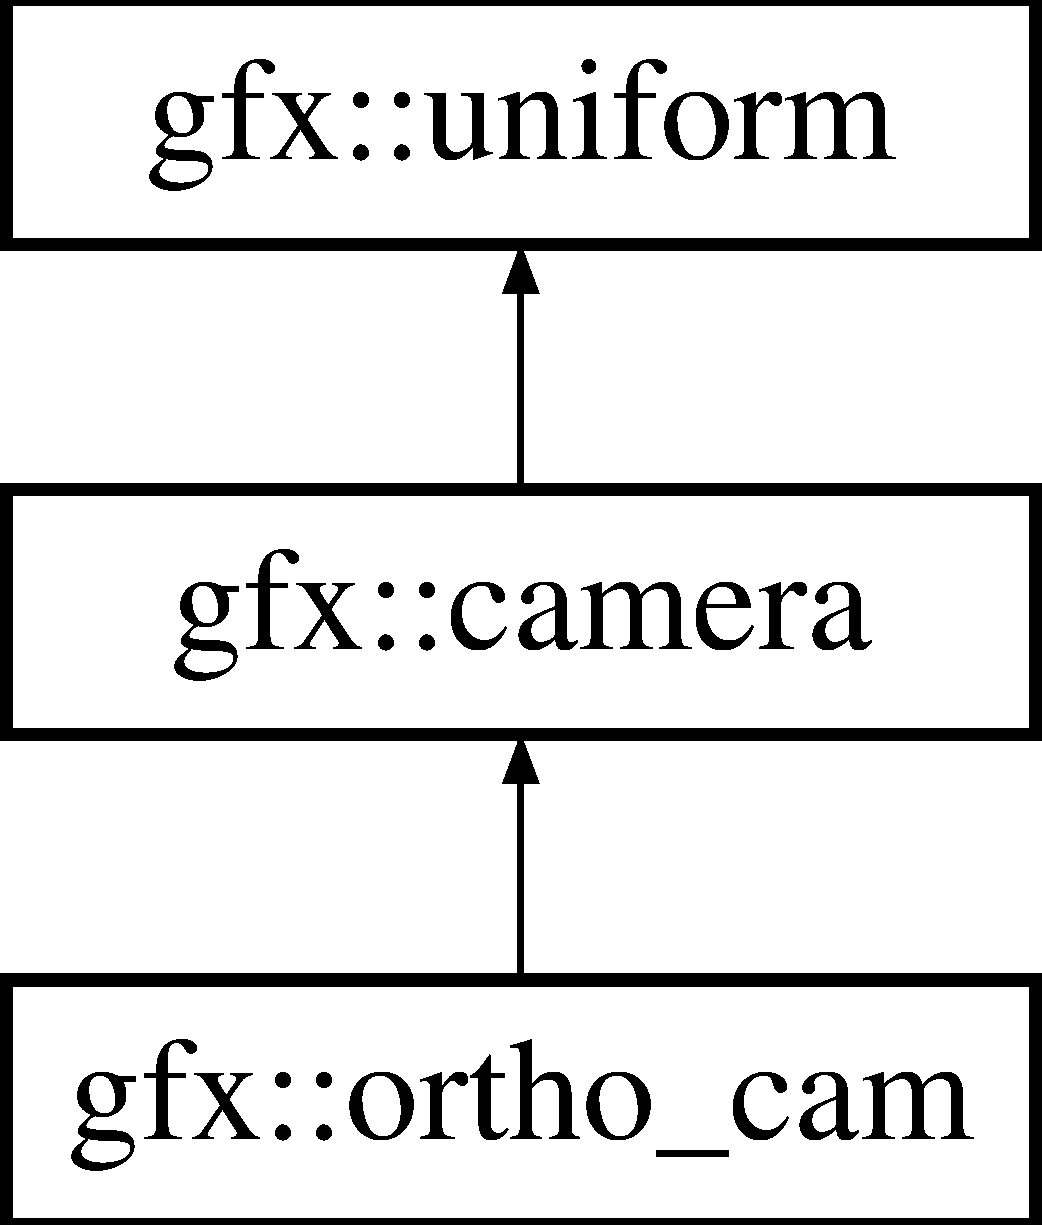
\includegraphics[height=3.000000cm]{classgfx_1_1ortho__cam}
\end{center}
\end{figure}
\subsection*{Classes}
\begin{DoxyCompactItemize}
\item 
class \hyperlink{classgfx_1_1ortho__cam_1_1settings}{settings}
\end{DoxyCompactItemize}
\subsection*{Public Member Functions}
\begin{DoxyCompactItemize}
\item 
\hyperlink{classgfx_1_1ortho__cam_a02874bea9d05ea281cf2cb55142a62a9}{ortho\-\_\-cam} (\hyperlink{classgfx_1_1ortho__cam_1_1settings}{settings} const \&set=\hyperlink{classgfx_1_1ortho__cam_1_1settings}{settings}())
\begin{DoxyCompactList}\small\item\em Construct a new orthographic camera. \end{DoxyCompactList}\item 
\hypertarget{classgfx_1_1ortho__cam_a8f711f78d347d0a99a1f8b2333701656}{\hyperlink{classgfx_1_1ortho__cam_a8f711f78d347d0a99a1f8b2333701656}{$\sim$ortho\-\_\-cam} ()}\label{classgfx_1_1ortho__cam_a8f711f78d347d0a99a1f8b2333701656}

\begin{DoxyCompactList}\small\item\em Destruct this orthographic camera. \end{DoxyCompactList}\item 
\hyperlink{classgfx_1_1ortho__cam}{ortho\-\_\-cam} \& \hyperlink{classgfx_1_1ortho__cam_afe5471d3a7e35115185f571d4b238fba}{position} (vec3 const \&point)
\begin{DoxyCompactList}\small\item\em Set the orthographic camera's position. \end{DoxyCompactList}\item 
\hyperlink{classgfx_1_1ortho__cam}{ortho\-\_\-cam} \& \hyperlink{classgfx_1_1ortho__cam_afc22b44b9120637c92c3a358b2a54a1b}{look\-\_\-at} (vec3 const \&point)
\begin{DoxyCompactList}\small\item\em Set the point the orthographic camera looks at. \end{DoxyCompactList}\item 
\hyperlink{classgfx_1_1ortho__cam}{ortho\-\_\-cam} \& \hyperlink{classgfx_1_1ortho__cam_a23d29a456f8127e1e88ca5517f3cd50a}{upward} (vec3 const \&dir)
\begin{DoxyCompactList}\small\item\em Set the direction the orthographic camera considers to be up. \end{DoxyCompactList}\item 
\hyperlink{classgfx_1_1ortho__cam}{ortho\-\_\-cam} \& \hyperlink{classgfx_1_1ortho__cam_a08d859c4ab06a0bcb0ffcd0221b321bb}{aspect\-\_\-ratio} (double ar)
\begin{DoxyCompactList}\small\item\em Set the orthographic camera's aspect ratio. \end{DoxyCompactList}\item 
\hyperlink{classgfx_1_1ortho__cam}{ortho\-\_\-cam} \& \hyperlink{classgfx_1_1ortho__cam_ac7760e5bad7dd1eaf2440bdc1c451c6f}{scale} (double scl)
\begin{DoxyCompactList}\small\item\em Set the orthographic camera's scale. \end{DoxyCompactList}\item 
\hyperlink{classgfx_1_1ortho__cam}{ortho\-\_\-cam} \& \hyperlink{classgfx_1_1ortho__cam_af8236f4efd294a6d4c559e2efb51c37c}{far\-\_\-plane} (double fp)
\begin{DoxyCompactList}\small\item\em Set the orthographic camera's far clipping plane. \end{DoxyCompactList}\end{DoxyCompactItemize}
\subsection*{Protected Member Functions}
\begin{DoxyCompactItemize}
\item 
\hypertarget{classgfx_1_1ortho__cam_a80f461508ab2b71d39c938beef5c57ba}{virtual void \hyperlink{classgfx_1_1ortho__cam_a80f461508ab2b71d39c938beef5c57ba}{update\-\_\-view} ()}\label{classgfx_1_1ortho__cam_a80f461508ab2b71d39c938beef5c57ba}

\begin{DoxyCompactList}\small\item\em Update the view matrix of the orthographic camera. Used internally. \end{DoxyCompactList}\end{DoxyCompactItemize}
\subsection*{Protected Attributes}
\begin{DoxyCompactItemize}
\item 
\hypertarget{classgfx_1_1ortho__cam_a754d9a39e56434721ee305e5a0f53e45}{vec3 {\bfseries pos}}\label{classgfx_1_1ortho__cam_a754d9a39e56434721ee305e5a0f53e45}

\item 
\hypertarget{classgfx_1_1ortho__cam_a4de4fd1c9e79446f1f7266d90217b2b4}{vec3 {\bfseries look}}\label{classgfx_1_1ortho__cam_a4de4fd1c9e79446f1f7266d90217b2b4}

\item 
\hypertarget{classgfx_1_1ortho__cam_a1b630086ab9e20fde6f4fd47e959f6c3}{vec3 {\bfseries up}}\label{classgfx_1_1ortho__cam_a1b630086ab9e20fde6f4fd47e959f6c3}

\item 
\hypertarget{classgfx_1_1ortho__cam_ae91d2750eb32b7e33253d7662b3b5926}{double {\bfseries aspect}}\label{classgfx_1_1ortho__cam_ae91d2750eb32b7e33253d7662b3b5926}

\item 
\hypertarget{classgfx_1_1ortho__cam_af53282509fb8f01997ef2b2c98fe9a0b}{double {\bfseries scale\-\_\-v}}\label{classgfx_1_1ortho__cam_af53282509fb8f01997ef2b2c98fe9a0b}

\item 
\hypertarget{classgfx_1_1ortho__cam_af8c46db72c1f5075f4533a8ecb728011}{double {\bfseries far}}\label{classgfx_1_1ortho__cam_af8c46db72c1f5075f4533a8ecb728011}

\item 
\hypertarget{classgfx_1_1ortho__cam_a2eb528597e124a0ac86d53664bd4eace}{mat4 {\bfseries scale\-\_\-m}}\label{classgfx_1_1ortho__cam_a2eb528597e124a0ac86d53664bd4eace}

\item 
\hypertarget{classgfx_1_1ortho__cam_a295e58950ed5407289d4961076a8b3f1}{bool {\bfseries volume\-\_\-changed}}\label{classgfx_1_1ortho__cam_a295e58950ed5407289d4961076a8b3f1}

\end{DoxyCompactItemize}


\subsection{Detailed Description}
An orthographic camera. 

Functions just like a \hyperlink{classgfx_1_1proj__cam}{proj\-\_\-cam}, but with no persepctive, instead using a scaling factor. 

\subsection{Constructor \& Destructor Documentation}
\hypertarget{classgfx_1_1ortho__cam_a02874bea9d05ea281cf2cb55142a62a9}{\index{gfx\-::ortho\-\_\-cam@{gfx\-::ortho\-\_\-cam}!ortho\-\_\-cam@{ortho\-\_\-cam}}
\index{ortho\-\_\-cam@{ortho\-\_\-cam}!gfx::ortho_cam@{gfx\-::ortho\-\_\-cam}}
\subsubsection[{ortho\-\_\-cam}]{\setlength{\rightskip}{0pt plus 5cm}gfx\-::ortho\-\_\-cam\-::ortho\-\_\-cam (
\begin{DoxyParamCaption}
\item[{{\bf settings} const \&}]{set = {\ttfamily {\bf settings}()}}
\end{DoxyParamCaption}
)}}\label{classgfx_1_1ortho__cam_a02874bea9d05ea281cf2cb55142a62a9}


Construct a new orthographic camera. 


\begin{DoxyParams}{Parameters}
{\em set} & The settings for the new orthographic camera \\
\hline
\end{DoxyParams}


\subsection{Member Function Documentation}
\hypertarget{classgfx_1_1ortho__cam_a08d859c4ab06a0bcb0ffcd0221b321bb}{\index{gfx\-::ortho\-\_\-cam@{gfx\-::ortho\-\_\-cam}!aspect\-\_\-ratio@{aspect\-\_\-ratio}}
\index{aspect\-\_\-ratio@{aspect\-\_\-ratio}!gfx::ortho_cam@{gfx\-::ortho\-\_\-cam}}
\subsubsection[{aspect\-\_\-ratio}]{\setlength{\rightskip}{0pt plus 5cm}{\bf ortho\-\_\-cam} \& gfx\-::ortho\-\_\-cam\-::aspect\-\_\-ratio (
\begin{DoxyParamCaption}
\item[{double}]{ar}
\end{DoxyParamCaption}
)}}\label{classgfx_1_1ortho__cam_a08d859c4ab06a0bcb0ffcd0221b321bb}


Set the orthographic camera's aspect ratio. 


\begin{DoxyParams}{Parameters}
{\em vert} & The aspect ratio \\
\hline
\end{DoxyParams}
\begin{DoxyReturn}{Returns}
This orthographic camera 
\end{DoxyReturn}
\hypertarget{classgfx_1_1ortho__cam_af8236f4efd294a6d4c559e2efb51c37c}{\index{gfx\-::ortho\-\_\-cam@{gfx\-::ortho\-\_\-cam}!far\-\_\-plane@{far\-\_\-plane}}
\index{far\-\_\-plane@{far\-\_\-plane}!gfx::ortho_cam@{gfx\-::ortho\-\_\-cam}}
\subsubsection[{far\-\_\-plane}]{\setlength{\rightskip}{0pt plus 5cm}{\bf ortho\-\_\-cam} \& gfx\-::ortho\-\_\-cam\-::far\-\_\-plane (
\begin{DoxyParamCaption}
\item[{double}]{fp}
\end{DoxyParamCaption}
)}}\label{classgfx_1_1ortho__cam_af8236f4efd294a6d4c559e2efb51c37c}


Set the orthographic camera's far clipping plane. 


\begin{DoxyParams}{Parameters}
{\em fp} & The distance to the far clipping plane \\
\hline
\end{DoxyParams}
\begin{DoxyReturn}{Returns}
This orthographic camera 
\end{DoxyReturn}
\hypertarget{classgfx_1_1ortho__cam_afc22b44b9120637c92c3a358b2a54a1b}{\index{gfx\-::ortho\-\_\-cam@{gfx\-::ortho\-\_\-cam}!look\-\_\-at@{look\-\_\-at}}
\index{look\-\_\-at@{look\-\_\-at}!gfx::ortho_cam@{gfx\-::ortho\-\_\-cam}}
\subsubsection[{look\-\_\-at}]{\setlength{\rightskip}{0pt plus 5cm}{\bf ortho\-\_\-cam} \& gfx\-::ortho\-\_\-cam\-::look\-\_\-at (
\begin{DoxyParamCaption}
\item[{vec3 const \&}]{point}
\end{DoxyParamCaption}
)}}\label{classgfx_1_1ortho__cam_afc22b44b9120637c92c3a358b2a54a1b}


Set the point the orthographic camera looks at. 


\begin{DoxyParams}{Parameters}
{\em point} & The point the orthographic camera looks at \\
\hline
\end{DoxyParams}
\begin{DoxyReturn}{Returns}
This orthographic camera 
\end{DoxyReturn}
\hypertarget{classgfx_1_1ortho__cam_afe5471d3a7e35115185f571d4b238fba}{\index{gfx\-::ortho\-\_\-cam@{gfx\-::ortho\-\_\-cam}!position@{position}}
\index{position@{position}!gfx::ortho_cam@{gfx\-::ortho\-\_\-cam}}
\subsubsection[{position}]{\setlength{\rightskip}{0pt plus 5cm}{\bf ortho\-\_\-cam} \& gfx\-::ortho\-\_\-cam\-::position (
\begin{DoxyParamCaption}
\item[{vec3 const \&}]{point}
\end{DoxyParamCaption}
)}}\label{classgfx_1_1ortho__cam_afe5471d3a7e35115185f571d4b238fba}


Set the orthographic camera's position. 


\begin{DoxyParams}{Parameters}
{\em point} & The position of the orthographic camera \\
\hline
\end{DoxyParams}
\begin{DoxyReturn}{Returns}
This orthographic camera 
\end{DoxyReturn}
\hypertarget{classgfx_1_1ortho__cam_ac7760e5bad7dd1eaf2440bdc1c451c6f}{\index{gfx\-::ortho\-\_\-cam@{gfx\-::ortho\-\_\-cam}!scale@{scale}}
\index{scale@{scale}!gfx::ortho_cam@{gfx\-::ortho\-\_\-cam}}
\subsubsection[{scale}]{\setlength{\rightskip}{0pt plus 5cm}{\bf ortho\-\_\-cam} \& gfx\-::ortho\-\_\-cam\-::scale (
\begin{DoxyParamCaption}
\item[{double}]{scl}
\end{DoxyParamCaption}
)}}\label{classgfx_1_1ortho__cam_ac7760e5bad7dd1eaf2440bdc1c451c6f}


Set the orthographic camera's scale. 


\begin{DoxyParams}{Parameters}
{\em vert} & The scale \\
\hline
\end{DoxyParams}
\begin{DoxyReturn}{Returns}
This orthographic camera 
\end{DoxyReturn}
\hypertarget{classgfx_1_1ortho__cam_a23d29a456f8127e1e88ca5517f3cd50a}{\index{gfx\-::ortho\-\_\-cam@{gfx\-::ortho\-\_\-cam}!upward@{upward}}
\index{upward@{upward}!gfx::ortho_cam@{gfx\-::ortho\-\_\-cam}}
\subsubsection[{upward}]{\setlength{\rightskip}{0pt plus 5cm}{\bf ortho\-\_\-cam} \& gfx\-::ortho\-\_\-cam\-::upward (
\begin{DoxyParamCaption}
\item[{vec3 const \&}]{dir}
\end{DoxyParamCaption}
)}}\label{classgfx_1_1ortho__cam_a23d29a456f8127e1e88ca5517f3cd50a}


Set the direction the orthographic camera considers to be up. 


\begin{DoxyParams}{Parameters}
{\em dir} & The direction that the orthographic camera considers to be up \\
\hline
\end{DoxyParams}
\begin{DoxyReturn}{Returns}
This orthographic camera 
\end{DoxyReturn}


The documentation for this class was generated from the following files\-:\begin{DoxyCompactItemize}
\item 
g\-Scene/camera.\-hpp\item 
g\-Scene/camera.\-cpp\end{DoxyCompactItemize}

\hypertarget{classgfx_1_1point__light}{\section{gfx\-:\-:point\-\_\-light Class Reference}
\label{classgfx_1_1point__light}\index{gfx\-::point\-\_\-light@{gfx\-::point\-\_\-light}}
}


A representation of a point light.  




{\ttfamily \#include \char`\"{}g\-Core/g\-Video/light.\-hpp\char`\"{}}

Inheritance diagram for gfx\-:\-:point\-\_\-light\-:\begin{figure}[H]
\begin{center}
\leavevmode
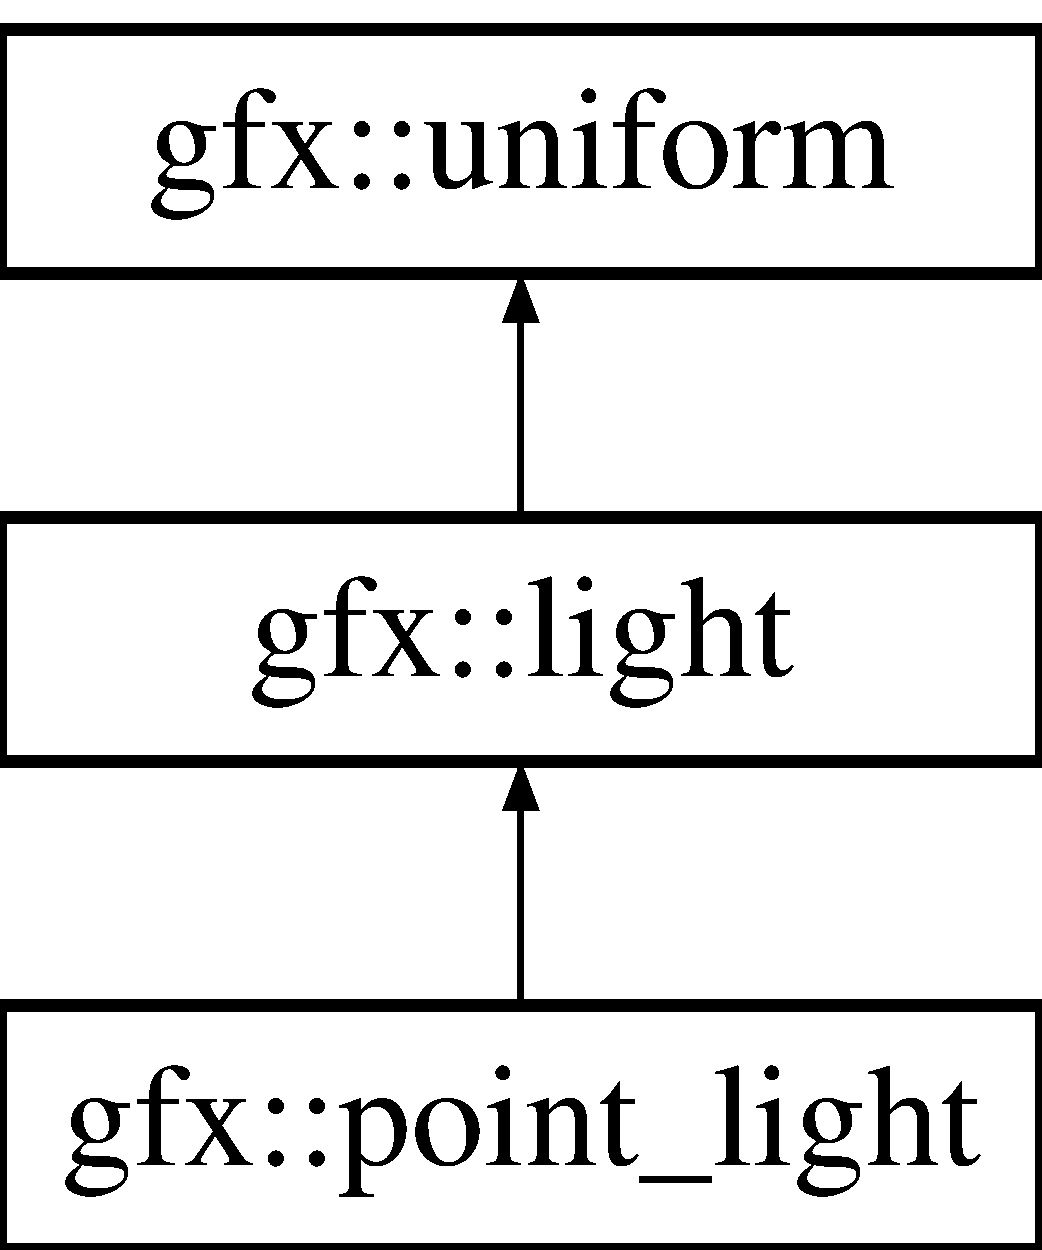
\includegraphics[height=3.000000cm]{classgfx_1_1point__light}
\end{center}
\end{figure}
\subsection*{Classes}
\begin{DoxyCompactItemize}
\item 
class \hyperlink{classgfx_1_1point__light_1_1settings}{settings}
\end{DoxyCompactItemize}
\subsection*{Public Member Functions}
\begin{DoxyCompactItemize}
\item 
\hyperlink{classgfx_1_1point__light_adeb313976364f094bff0cd8086b3ec3c}{point\-\_\-light} (\hyperlink{classgfx_1_1point__light_1_1settings}{settings} const \&set=\hyperlink{classgfx_1_1point__light_1_1settings}{settings}())
\begin{DoxyCompactList}\small\item\em Construct a new point light object. \end{DoxyCompactList}\item 
\hyperlink{classgfx_1_1point__light}{point\-\_\-light} \& \hyperlink{classgfx_1_1point__light_ad0e0fa27a2136f000e1e30de07309697}{position} (vec3 const \&pos)
\begin{DoxyCompactList}\small\item\em Set the position to the given value. \end{DoxyCompactList}\item 
vec3 const \& \hyperlink{classgfx_1_1point__light_a0794f094bebf222bc6b379fc31b26bf1}{position} () const 
\begin{DoxyCompactList}\small\item\em Return the point light's position. \end{DoxyCompactList}\item 
\hyperlink{classgfx_1_1point__light}{point\-\_\-light} \& \hyperlink{classgfx_1_1point__light_a3f481861cb135d189f4e65c2cf184547}{color} (vec3 const \&col)
\begin{DoxyCompactList}\small\item\em Set the color to the given value. \end{DoxyCompactList}\item 
vec3 const \& \hyperlink{classgfx_1_1point__light_a376b6bfddbb471eabca4a69042f35a91}{color} () const 
\begin{DoxyCompactList}\small\item\em Return the point light's color. \end{DoxyCompactList}\item 
virtual void \hyperlink{classgfx_1_1point__light_a9549403e263927018c000f857cb1e718}{upload\-\_\-uniform} (\hyperlink{classgfx_1_1program}{program} \&prgm, std\-::string const \&name)
\begin{DoxyCompactList}\small\item\em Upload this point light as a uniform to the given \hyperlink{classgfx_1_1program}{program}. \end{DoxyCompactList}\end{DoxyCompactItemize}
\subsection*{Protected Attributes}
\begin{DoxyCompactItemize}
\item 
\hypertarget{classgfx_1_1point__light_aed8ad3ac893e2a6cee2b60273362dc0b}{vec3 {\bfseries pos}}\label{classgfx_1_1point__light_aed8ad3ac893e2a6cee2b60273362dc0b}

\item 
\hypertarget{classgfx_1_1point__light_a918bc9997234187a2de7f90492e8e3ef}{vec3 {\bfseries col}}\label{classgfx_1_1point__light_a918bc9997234187a2de7f90492e8e3ef}

\end{DoxyCompactItemize}
\subsection*{Additional Inherited Members}


\subsection{Detailed Description}
A representation of a point light. 

This light has color and position as well as radiance. 

\subsection{Constructor \& Destructor Documentation}
\hypertarget{classgfx_1_1point__light_adeb313976364f094bff0cd8086b3ec3c}{\index{gfx\-::point\-\_\-light@{gfx\-::point\-\_\-light}!point\-\_\-light@{point\-\_\-light}}
\index{point\-\_\-light@{point\-\_\-light}!gfx::point_light@{gfx\-::point\-\_\-light}}
\subsubsection[{point\-\_\-light}]{\setlength{\rightskip}{0pt plus 5cm}gfx\-::point\-\_\-light\-::point\-\_\-light (
\begin{DoxyParamCaption}
\item[{{\bf settings} const \&}]{set = {\ttfamily {\bf settings}()}}
\end{DoxyParamCaption}
)}}\label{classgfx_1_1point__light_adeb313976364f094bff0cd8086b3ec3c}


Construct a new point light object. 


\begin{DoxyParams}{Parameters}
{\em set} & The settings for the new point light. \\
\hline
\end{DoxyParams}


\subsection{Member Function Documentation}
\hypertarget{classgfx_1_1point__light_a3f481861cb135d189f4e65c2cf184547}{\index{gfx\-::point\-\_\-light@{gfx\-::point\-\_\-light}!color@{color}}
\index{color@{color}!gfx::point_light@{gfx\-::point\-\_\-light}}
\subsubsection[{color}]{\setlength{\rightskip}{0pt plus 5cm}{\bf point\-\_\-light} \& gfx\-::point\-\_\-light\-::color (
\begin{DoxyParamCaption}
\item[{vec3 const \&}]{col}
\end{DoxyParamCaption}
)}}\label{classgfx_1_1point__light_a3f481861cb135d189f4e65c2cf184547}


Set the color to the given value. 


\begin{DoxyParams}{Parameters}
{\em col} & The color of the point light \\
\hline
\end{DoxyParams}
\begin{DoxyReturn}{Returns}
This point light object 
\end{DoxyReturn}
\hypertarget{classgfx_1_1point__light_a376b6bfddbb471eabca4a69042f35a91}{\index{gfx\-::point\-\_\-light@{gfx\-::point\-\_\-light}!color@{color}}
\index{color@{color}!gfx::point_light@{gfx\-::point\-\_\-light}}
\subsubsection[{color}]{\setlength{\rightskip}{0pt plus 5cm}vec3 const \& gfx\-::point\-\_\-light\-::color (
\begin{DoxyParamCaption}
{}
\end{DoxyParamCaption}
) const}}\label{classgfx_1_1point__light_a376b6bfddbb471eabca4a69042f35a91}


Return the point light's color. 

\begin{DoxyReturn}{Returns}
The color of the point light object. 
\end{DoxyReturn}
\hypertarget{classgfx_1_1point__light_ad0e0fa27a2136f000e1e30de07309697}{\index{gfx\-::point\-\_\-light@{gfx\-::point\-\_\-light}!position@{position}}
\index{position@{position}!gfx::point_light@{gfx\-::point\-\_\-light}}
\subsubsection[{position}]{\setlength{\rightskip}{0pt plus 5cm}{\bf point\-\_\-light} \& gfx\-::point\-\_\-light\-::position (
\begin{DoxyParamCaption}
\item[{vec3 const \&}]{pos}
\end{DoxyParamCaption}
)}}\label{classgfx_1_1point__light_ad0e0fa27a2136f000e1e30de07309697}


Set the position to the given value. 


\begin{DoxyParams}{Parameters}
{\em pos} & The position of the point light \\
\hline
\end{DoxyParams}
\begin{DoxyReturn}{Returns}
This point light object 
\end{DoxyReturn}
\hypertarget{classgfx_1_1point__light_a0794f094bebf222bc6b379fc31b26bf1}{\index{gfx\-::point\-\_\-light@{gfx\-::point\-\_\-light}!position@{position}}
\index{position@{position}!gfx::point_light@{gfx\-::point\-\_\-light}}
\subsubsection[{position}]{\setlength{\rightskip}{0pt plus 5cm}vec3 const \& gfx\-::point\-\_\-light\-::position (
\begin{DoxyParamCaption}
{}
\end{DoxyParamCaption}
) const}}\label{classgfx_1_1point__light_a0794f094bebf222bc6b379fc31b26bf1}


Return the point light's position. 

\begin{DoxyReturn}{Returns}
The position of the point light object. 
\end{DoxyReturn}
\hypertarget{classgfx_1_1point__light_a9549403e263927018c000f857cb1e718}{\index{gfx\-::point\-\_\-light@{gfx\-::point\-\_\-light}!upload\-\_\-uniform@{upload\-\_\-uniform}}
\index{upload\-\_\-uniform@{upload\-\_\-uniform}!gfx::point_light@{gfx\-::point\-\_\-light}}
\subsubsection[{upload\-\_\-uniform}]{\setlength{\rightskip}{0pt plus 5cm}void gfx\-::point\-\_\-light\-::upload\-\_\-uniform (
\begin{DoxyParamCaption}
\item[{{\bf program} \&}]{prgm, }
\item[{std\-::string const \&}]{name}
\end{DoxyParamCaption}
)\hspace{0.3cm}{\ttfamily [virtual]}}}\label{classgfx_1_1point__light_a9549403e263927018c000f857cb1e718}


Upload this point light as a uniform to the given \hyperlink{classgfx_1_1program}{program}. 

\begin{DoxyRefDesc}{Todo}
\item[\hyperlink{todo__todo000020}{Todo}]The uniform class and programs aren't smart enough, yet, for this to work properly. Some shenanigans using an updated info and type system is needed. \end{DoxyRefDesc}


Reimplemented from \hyperlink{classgfx_1_1light_a7b974f1340562d8740192b2ff0d62f93}{gfx\-::light}.



The documentation for this class was generated from the following files\-:\begin{DoxyCompactItemize}
\item 
g\-Scene/light.\-hpp\item 
g\-Scene/light.\-cpp\end{DoxyCompactItemize}

\hypertarget{classgfx_1_1primitive}{\section{gfx\-:\-:primitive Class Reference}
\label{classgfx_1_1primitive}\index{gfx\-::primitive@{gfx\-::primitive}}
}


An interface for basic shapes.  




{\ttfamily \#include \char`\"{}g\-Core/g\-Scene/primitivie.\-hpp\char`\"{}}

Inheritance diagram for gfx\-:\-:primitive\-:\begin{figure}[H]
\begin{center}
\leavevmode
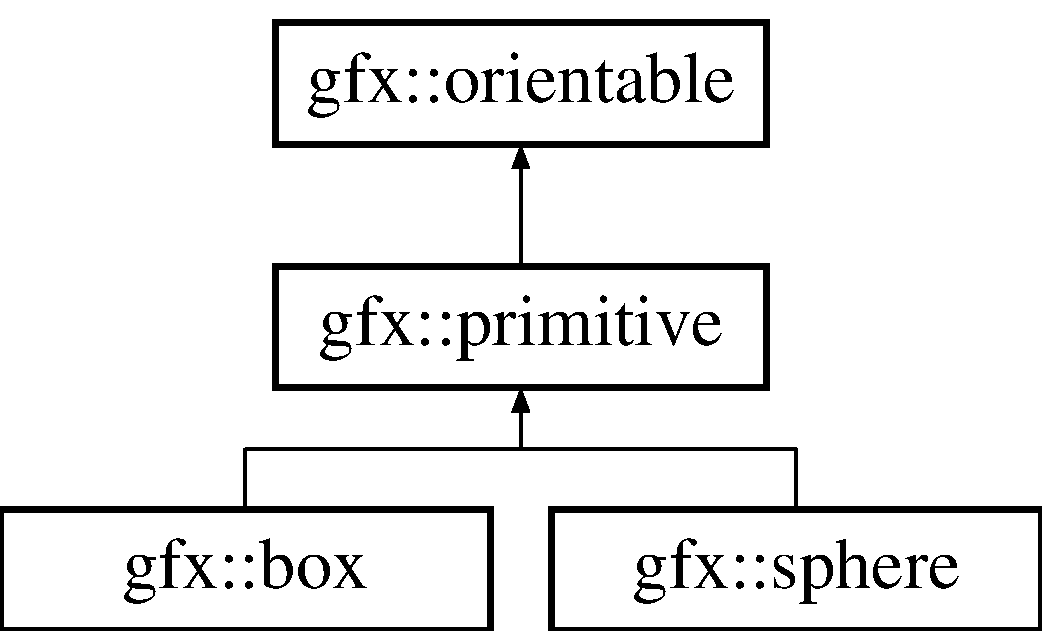
\includegraphics[height=3.000000cm]{classgfx_1_1primitive}
\end{center}
\end{figure}
\subsection*{Classes}
\begin{DoxyCompactItemize}
\item 
class \hyperlink{classgfx_1_1primitive_1_1settings}{settings}
\end{DoxyCompactItemize}
\subsection*{Public Member Functions}
\begin{DoxyCompactItemize}
\item 
\hypertarget{classgfx_1_1primitive_a30e7e1030b859a0a322b3be3aa8913c8}{{\bfseries primitive} (\hyperlink{classgfx_1_1primitive_1_1settings}{settings} const \&set=\hyperlink{classgfx_1_1primitive_1_1settings}{settings}())}\label{classgfx_1_1primitive_a30e7e1030b859a0a322b3be3aa8913c8}

\item 
\hypertarget{classgfx_1_1primitive_a243e48daedff5cc42f4f9a6bedfbb584}{virtual \hyperlink{classgfx_1_1buffer}{buffer} const \& {\bfseries geometry} () const =0}\label{classgfx_1_1primitive_a243e48daedff5cc42f4f9a6bedfbb584}

\end{DoxyCompactItemize}
\subsection*{Additional Inherited Members}


\subsection{Detailed Description}
An interface for basic shapes. 

Primitives have geometry that is set and can only be manipulated by changing the transformation matrix provided by the base class \hyperlink{classgfx_1_1orientable}{orientable}. 

The documentation for this class was generated from the following file\-:\begin{DoxyCompactItemize}
\item 
g\-Scene/primitive.\-hpp\end{DoxyCompactItemize}

\hypertarget{classgfx_1_1process__cam}{\section{gfx\-:\-:process\-\_\-cam Class Reference}
\label{classgfx_1_1process__cam}\index{gfx\-::process\-\_\-cam@{gfx\-::process\-\_\-cam}}
}


A camera for 'process work'.  




{\ttfamily \#include \char`\"{}g\-Core/g\-Scene/camera.\-hpp\char`\"{}}

Inheritance diagram for gfx\-:\-:process\-\_\-cam\-:\begin{figure}[H]
\begin{center}
\leavevmode
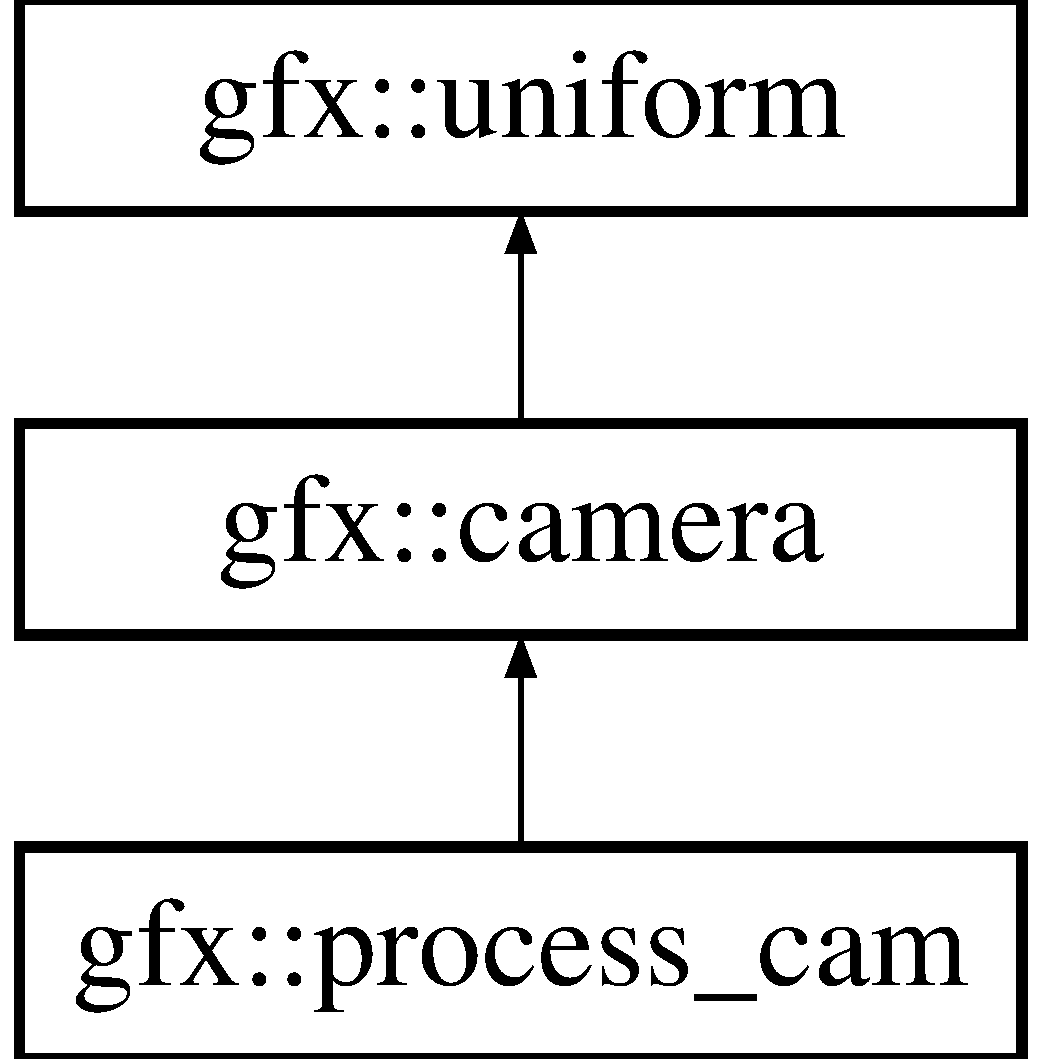
\includegraphics[height=3.000000cm]{classgfx_1_1process__cam}
\end{center}
\end{figure}
\subsection*{Classes}
\begin{DoxyCompactItemize}
\item 
class \hyperlink{classgfx_1_1process__cam_1_1settings}{settings}
\end{DoxyCompactItemize}
\subsection*{Public Member Functions}
\begin{DoxyCompactItemize}
\item 
\hyperlink{classgfx_1_1process__cam_ae8140987d24060b32d38af0c974db57d}{process\-\_\-cam} (\hyperlink{classgfx_1_1process__cam_1_1settings}{settings} const \&set=\hyperlink{classgfx_1_1process__cam_1_1settings}{settings}())
\begin{DoxyCompactList}\small\item\em Construct a new process camera. \end{DoxyCompactList}\item 
\hypertarget{classgfx_1_1process__cam_ae37352650ea0f73fc5e896c0d2ac93b9}{\hyperlink{classgfx_1_1process__cam_ae37352650ea0f73fc5e896c0d2ac93b9}{$\sim$process\-\_\-cam} ()}\label{classgfx_1_1process__cam_ae37352650ea0f73fc5e896c0d2ac93b9}

\begin{DoxyCompactList}\small\item\em Destruct this process camera. \end{DoxyCompactList}\item 
\hyperlink{classgfx_1_1process__cam}{process\-\_\-cam} \& \hyperlink{classgfx_1_1process__cam_ab2f973b728a87300d284bc2a84b99d9f}{mask\-\_\-region} (vec2 const \&ul\-\_\-corner, vec2 const \&lr\-\_\-corner)
\begin{DoxyCompactList}\small\item\em Set the extent of the process camera's masking region. \end{DoxyCompactList}\item 
\hyperlink{classgfx_1_1process__cam}{process\-\_\-cam} \& \hyperlink{classgfx_1_1process__cam_a606398d6801ce89cedcf2db7762dd6a7}{screen\-\_\-region} (vec2 const \&ul\-\_\-corner, vec2 const \&lr\-\_\-corner)
\begin{DoxyCompactList}\small\item\em Set the full extent of the process camera's renderable area. \end{DoxyCompactList}\end{DoxyCompactItemize}
\subsection*{Protected Member Functions}
\begin{DoxyCompactItemize}
\item 
virtual void \hyperlink{classgfx_1_1process__cam_abf4a9226e8d0907b70f3eadc2b4229a5}{update\-\_\-view} ()
\begin{DoxyCompactList}\small\item\em Update the view matrix of the process camera. Used internally. \end{DoxyCompactList}\end{DoxyCompactItemize}
\subsection*{Protected Attributes}
\begin{DoxyCompactItemize}
\item 
\hypertarget{classgfx_1_1process__cam_a87a0f257f8be74bd2e2263bed73c29d2}{vec4 {\bfseries mask}}\label{classgfx_1_1process__cam_a87a0f257f8be74bd2e2263bed73c29d2}

\item 
\hypertarget{classgfx_1_1process__cam_ae643f7cb3a0da2b13564ce4914df5fb7}{vec4 {\bfseries screen}}\label{classgfx_1_1process__cam_ae643f7cb3a0da2b13564ce4914df5fb7}

\item 
\hypertarget{classgfx_1_1process__cam_a9de84c9a868e246d615afc5029af7f7c}{mat4 {\bfseries clip\-\_\-m}}\label{classgfx_1_1process__cam_a9de84c9a868e246d615afc5029af7f7c}

\item 
\hypertarget{classgfx_1_1process__cam_a74ce3b70400f3de5038e15bbc91a6519}{bool {\bfseries clip\-\_\-changed}}\label{classgfx_1_1process__cam_a74ce3b70400f3de5038e15bbc91a6519}

\end{DoxyCompactItemize}


\subsection{Detailed Description}
A camera for 'process work'. 

That is, compositing and rendering mattes and elements to the screen. The mask region is the sub area of the plane \mbox{[}-\/1,1\mbox{]}\mbox{[}-\/1,1\mbox{]} to project and the screen region is the sub area of the renderbuffer to project to. 

\subsection{Constructor \& Destructor Documentation}
\hypertarget{classgfx_1_1process__cam_ae8140987d24060b32d38af0c974db57d}{\index{gfx\-::process\-\_\-cam@{gfx\-::process\-\_\-cam}!process\-\_\-cam@{process\-\_\-cam}}
\index{process\-\_\-cam@{process\-\_\-cam}!gfx::process_cam@{gfx\-::process\-\_\-cam}}
\subsubsection[{process\-\_\-cam}]{\setlength{\rightskip}{0pt plus 5cm}gfx\-::process\-\_\-cam\-::process\-\_\-cam (
\begin{DoxyParamCaption}
\item[{{\bf settings} const \&}]{set = {\ttfamily {\bf settings}()}}
\end{DoxyParamCaption}
)}}\label{classgfx_1_1process__cam_ae8140987d24060b32d38af0c974db57d}


Construct a new process camera. 


\begin{DoxyParams}{Parameters}
{\em set} & The settings for the new process camera \\
\hline
\end{DoxyParams}


\subsection{Member Function Documentation}
\hypertarget{classgfx_1_1process__cam_ab2f973b728a87300d284bc2a84b99d9f}{\index{gfx\-::process\-\_\-cam@{gfx\-::process\-\_\-cam}!mask\-\_\-region@{mask\-\_\-region}}
\index{mask\-\_\-region@{mask\-\_\-region}!gfx::process_cam@{gfx\-::process\-\_\-cam}}
\subsubsection[{mask\-\_\-region}]{\setlength{\rightskip}{0pt plus 5cm}{\bf process\-\_\-cam} \& gfx\-::process\-\_\-cam\-::mask\-\_\-region (
\begin{DoxyParamCaption}
\item[{vec2 const \&}]{ul\-\_\-corner, }
\item[{vec2 const \&}]{lr\-\_\-corner}
\end{DoxyParamCaption}
)}}\label{classgfx_1_1process__cam_ab2f973b728a87300d284bc2a84b99d9f}


Set the extent of the process camera's masking region. 


\begin{DoxyParams}{Parameters}
{\em ul\-\_\-corner} & The upper left corner of the masking region \\
\hline
{\em lr\-\_\-corner} & The lower right corner of the masking region \\
\hline
\end{DoxyParams}
\begin{DoxyReturn}{Returns}
This process camera 
\end{DoxyReturn}
\hypertarget{classgfx_1_1process__cam_a606398d6801ce89cedcf2db7762dd6a7}{\index{gfx\-::process\-\_\-cam@{gfx\-::process\-\_\-cam}!screen\-\_\-region@{screen\-\_\-region}}
\index{screen\-\_\-region@{screen\-\_\-region}!gfx::process_cam@{gfx\-::process\-\_\-cam}}
\subsubsection[{screen\-\_\-region}]{\setlength{\rightskip}{0pt plus 5cm}{\bf process\-\_\-cam} \& gfx\-::process\-\_\-cam\-::screen\-\_\-region (
\begin{DoxyParamCaption}
\item[{vec2 const \&}]{ul\-\_\-corner, }
\item[{vec2 const \&}]{lr\-\_\-corner}
\end{DoxyParamCaption}
)}}\label{classgfx_1_1process__cam_a606398d6801ce89cedcf2db7762dd6a7}


Set the full extent of the process camera's renderable area. 


\begin{DoxyParams}{Parameters}
{\em ul\-\_\-corner} & The upper left corner of the renderable area \\
\hline
{\em lr\-\_\-corner} & The lower right corner of the renderable area \\
\hline
\end{DoxyParams}
\begin{DoxyReturn}{Returns}
This process camera 
\end{DoxyReturn}
\hypertarget{classgfx_1_1process__cam_abf4a9226e8d0907b70f3eadc2b4229a5}{\index{gfx\-::process\-\_\-cam@{gfx\-::process\-\_\-cam}!update\-\_\-view@{update\-\_\-view}}
\index{update\-\_\-view@{update\-\_\-view}!gfx::process_cam@{gfx\-::process\-\_\-cam}}
\subsubsection[{update\-\_\-view}]{\setlength{\rightskip}{0pt plus 5cm}void gfx\-::process\-\_\-cam\-::update\-\_\-view (
\begin{DoxyParamCaption}
{}
\end{DoxyParamCaption}
)\hspace{0.3cm}{\ttfamily [protected]}, {\ttfamily [virtual]}}}\label{classgfx_1_1process__cam_abf4a9226e8d0907b70f3eadc2b4229a5}


Update the view matrix of the process camera. Used internally. 

\begin{DoxyRefDesc}{Todo}
\item[\hyperlink{todo__todo000016}{Todo}]My internal comments indicate that this is totally broken. So fix it. \end{DoxyRefDesc}


Implements \hyperlink{classgfx_1_1camera}{gfx\-::camera}.



The documentation for this class was generated from the following files\-:\begin{DoxyCompactItemize}
\item 
g\-Scene/camera.\-hpp\item 
g\-Scene/camera.\-cpp\end{DoxyCompactItemize}

\hypertarget{classgfx_1_1program}{\section{gfx\-:\-:program Class Reference}
\label{classgfx_1_1program}\index{gfx\-::program@{gfx\-::program}}
}


A representation of an Open\-G\-L shading program.  




{\ttfamily \#include \char`\"{}g\-Core/g\-Scene/program.\-hpp\char`\"{}}

\subsection*{Classes}
\begin{DoxyCompactItemize}
\item 
class \hyperlink{classgfx_1_1program_1_1settings}{settings}
\begin{DoxyCompactList}\small\item\em Used for configuring a new \hyperlink{classgfx_1_1program}{program} object. \end{DoxyCompactList}\end{DoxyCompactItemize}
\subsection*{Public Member Functions}
\begin{DoxyCompactItemize}
\item 
\hyperlink{classgfx_1_1program_a5f3c772a1cfeedfbf605f07a6c5c2ced}{program} (\hyperlink{classgfx_1_1program_1_1settings}{settings} const \&set=\hyperlink{classgfx_1_1program_1_1settings}{settings}())
\begin{DoxyCompactList}\small\item\em Construct a new \hyperlink{classgfx_1_1program}{program} object. \end{DoxyCompactList}\item 
\hypertarget{classgfx_1_1program_a4a13d9cc7adce2250ce24332e68481f3}{\hyperlink{classgfx_1_1program_a4a13d9cc7adce2250ce24332e68481f3}{$\sim$program} ()}\label{classgfx_1_1program_a4a13d9cc7adce2250ce24332e68481f3}

\begin{DoxyCompactList}\small\item\em Destruct this \hyperlink{classgfx_1_1program}{program}. \end{DoxyCompactList}\item 
void \hyperlink{classgfx_1_1program_af26c121d657805935a542e3eb1320389}{uniform\-\_\-name} (std\-::string const \&name)
\begin{DoxyCompactList}\small\item\em Specify that this program has a uniform slot with the given name. \end{DoxyCompactList}\item 
\hypertarget{classgfx_1_1program_a30bd1c354331da8a752b37aceba11292}{std\-::string {\bfseries vertex\-\_\-path} () const }\label{classgfx_1_1program_a30bd1c354331da8a752b37aceba11292}

\item 
\hypertarget{classgfx_1_1program_ae81ef9ea75db894d3a0ad58b34229000}{std\-::string {\bfseries fragment\-\_\-path} () const }\label{classgfx_1_1program_ae81ef9ea75db894d3a0ad58b34229000}

\item 
\hypertarget{classgfx_1_1program_aeecb4ba118bae38aa087a1115ff01724}{std\-::string {\bfseries tesselation\-\_\-path} () const }\label{classgfx_1_1program_aeecb4ba118bae38aa087a1115ff01724}

\item 
\hypertarget{classgfx_1_1program_aa80f6f1a9f581f30c96fe2cc4c589cac}{std\-::string {\bfseries geometry\-\_\-path} () const }\label{classgfx_1_1program_aa80f6f1a9f581f30c96fe2cc4c589cac}

\item 
void \hyperlink{classgfx_1_1program_ab925e8e749e08329b745635c388c3428}{compile} ()
\begin{DoxyCompactList}\small\item\em Compile the shader source associated with this program. \end{DoxyCompactList}\item 
void \hyperlink{classgfx_1_1program_a1fc41748646f62dd4dd98c7e9d012166}{link} ()
\begin{DoxyCompactList}\small\item\em Link compiled shader stages into one program. \end{DoxyCompactList}\item 
{\footnotesize template$<$typename T $>$ }\\void \hyperlink{classgfx_1_1program_aaf1cf681d9a5a75d121b6dba5794dceb}{upload\-\_\-uniform} (std\-::string const \&name, T const \&val)
\begin{DoxyCompactList}\small\item\em Upload the given data as a uniform to the Open\-G\-L program object. \end{DoxyCompactList}\item 
\hypertarget{classgfx_1_1program_a94f585db55bbc7933f5d4a4bcfb7cfc0}{void \hyperlink{classgfx_1_1program_a94f585db55bbc7933f5d4a4bcfb7cfc0}{use} ()}\label{classgfx_1_1program_a94f585db55bbc7933f5d4a4bcfb7cfc0}

\begin{DoxyCompactList}\small\item\em Set Open\-G\-L to use this program for all subsquent drawing instructions. \end{DoxyCompactList}\item 
bool \hyperlink{classgfx_1_1program_a4ba4fb099649e8dce803195d0f692a51}{in\-\_\-use} () const 
\begin{DoxyCompactList}\small\item\em Query this \hyperlink{classgfx_1_1program}{program} object to see if it is currently in use by Open\-G\-L. \end{DoxyCompactList}\item 
bool \hyperlink{classgfx_1_1program_afe778007d42b9ecb15e7818037484204}{operator==} (\hyperlink{classgfx_1_1program}{program} const \&rhs) const 
\begin{DoxyCompactList}\small\item\em Compare this \hyperlink{classgfx_1_1program}{program} to the given one to see if it does represent the same Open\-G\-L shader program as the one given. \end{DoxyCompactList}\item 
bool \hyperlink{classgfx_1_1program_a7c5ac99f3cf6a70d72e8eb58786ce673}{operator!=} (\hyperlink{classgfx_1_1program}{program} const \&rhs) const 
\begin{DoxyCompactList}\small\item\em Compare this \hyperlink{classgfx_1_1program}{program} to the given one to see if it does not represent the same Open\-G\-L shader program as the one given. \end{DoxyCompactList}\item 
{\footnotesize template$<$$>$ }\\void \hyperlink{classgfx_1_1program_ab3b82ebb6938a0a23533d1222dcb3ab1}{upload\-\_\-uniform} (std\-::string const \&name, float32 const \&val)
\begin{DoxyCompactList}\small\item\em Upload the given float as a uniform to the Open\-G\-L program object. \end{DoxyCompactList}\item 
{\footnotesize template$<$$>$ }\\void \hyperlink{classgfx_1_1program_a7ba8ce9e2be0434dc848c60fbc2d726f}{upload\-\_\-uniform} (std\-::string const \&name, float const \&val)
\begin{DoxyCompactList}\small\item\em Upload the given primitive float as a uniform to the Open\-G\-L program object. \end{DoxyCompactList}\item 
{\footnotesize template$<$$>$ }\\void \hyperlink{classgfx_1_1program_a98aa73f11960573d78f8d80c71160d7e}{upload\-\_\-uniform} (std\-::string const \&name, vec2 const \&val)
\begin{DoxyCompactList}\small\item\em Upload the given vector as a uniform to the Open\-G\-L program object. \end{DoxyCompactList}\item 
{\footnotesize template$<$$>$ }\\void \hyperlink{classgfx_1_1program_a6c4bb82effb1e19d8becca1a28b6974b}{upload\-\_\-uniform} (std\-::string const \&name, vec3 const \&val)
\begin{DoxyCompactList}\small\item\em Upload the given vector as a uniform to the Open\-G\-L program object. \end{DoxyCompactList}\item 
{\footnotesize template$<$$>$ }\\void \hyperlink{classgfx_1_1program_ac793a14e1f7891ff840b44c322f48e98}{upload\-\_\-uniform} (std\-::string const \&name, vec4 const \&val)
\begin{DoxyCompactList}\small\item\em Upload the given vector as a uniform to the Open\-G\-L program object. \end{DoxyCompactList}\item 
{\footnotesize template$<$$>$ }\\void \hyperlink{classgfx_1_1program_a3e1e89ed2a5053d03134e16cef7efc35}{upload\-\_\-uniform} (std\-::string const \&name, int32 const \&val)
\begin{DoxyCompactList}\small\item\em Upload the given integer as a uniform to the Open\-G\-L program object. \end{DoxyCompactList}\item 
{\footnotesize template$<$$>$ }\\void \hyperlink{classgfx_1_1program_ad9557bb105ae536e08e602918bc43440}{upload\-\_\-uniform} (std\-::string const \&name, int const \&val)
\begin{DoxyCompactList}\small\item\em Upload the given primitive integer as a uniform to the Open\-G\-L program object. \end{DoxyCompactList}\item 
{\footnotesize template$<$$>$ }\\void \hyperlink{classgfx_1_1program_adaed8e864d24f21b0818ced33d842bce}{upload\-\_\-uniform} (std\-::string const \&name, ivec2 const \&val)
\begin{DoxyCompactList}\small\item\em Upload the given vector as a uniform to the Open\-G\-L program object. \end{DoxyCompactList}\item 
{\footnotesize template$<$$>$ }\\void \hyperlink{classgfx_1_1program_af0fdec8101081f406a12972c0508e98a}{upload\-\_\-uniform} (std\-::string const \&name, ivec3 const \&val)
\begin{DoxyCompactList}\small\item\em Upload the given vector as a uniform to the Open\-G\-L program object. \end{DoxyCompactList}\item 
{\footnotesize template$<$$>$ }\\void \hyperlink{classgfx_1_1program_a4bc1046502033fa9a32201a4ce0f4b41}{upload\-\_\-uniform} (std\-::string const \&name, ivec4 const \&val)
\begin{DoxyCompactList}\small\item\em Upload the given vector as a uniform to the Open\-G\-L program object. \end{DoxyCompactList}\item 
{\footnotesize template$<$$>$ }\\void \hyperlink{classgfx_1_1program_a8b2a8069224d9d4b46b8d1ba3502ce1f}{upload\-\_\-uniform} (std\-::string const \&name, uint32 const \&val)
\begin{DoxyCompactList}\small\item\em Upload the given integer as a uniform to the Open\-G\-L program object. \end{DoxyCompactList}\item 
{\footnotesize template$<$$>$ }\\void \hyperlink{classgfx_1_1program_ae139f17939de4b5d01795b10fecccec6}{upload\-\_\-uniform} (std\-::string const \&name, uint32\-\_\-t const \&val)
\begin{DoxyCompactList}\small\item\em Upload the given primitive integer as a uniform to the Open\-G\-L program object. \end{DoxyCompactList}\item 
{\footnotesize template$<$$>$ }\\void \hyperlink{classgfx_1_1program_a0a4fd0922e71ddd475f50dceffa3ba88}{upload\-\_\-uniform} (std\-::string const \&name, uvec2 const \&val)
\begin{DoxyCompactList}\small\item\em Upload the given vector as a uniform to the Open\-G\-L program object. \end{DoxyCompactList}\item 
{\footnotesize template$<$$>$ }\\void \hyperlink{classgfx_1_1program_a1a68c40e30f4c00639df2ce60eba6b80}{upload\-\_\-uniform} (std\-::string const \&name, uvec3 const \&val)
\begin{DoxyCompactList}\small\item\em Upload the given vector as a uniform to the Open\-G\-L program object. \end{DoxyCompactList}\item 
{\footnotesize template$<$$>$ }\\void \hyperlink{classgfx_1_1program_a2492cfa836006650d5de5c4a03b581b5}{upload\-\_\-uniform} (std\-::string const \&name, uvec4 const \&val)
\begin{DoxyCompactList}\small\item\em Upload the given vector as a uniform to the Open\-G\-L program object. \end{DoxyCompactList}\item 
{\footnotesize template$<$$>$ }\\void \hyperlink{classgfx_1_1program_ad7d4c6f5074ef425bd45ee71a74c1cd4}{upload\-\_\-uniform} (std\-::string const \&name, mat2 const \&val)
\begin{DoxyCompactList}\small\item\em Upload the given matrix as a uniform to the Open\-G\-L program object. \end{DoxyCompactList}\item 
{\footnotesize template$<$$>$ }\\void \hyperlink{classgfx_1_1program_ac85d00fb59623952cfec499ef34ae2e8}{upload\-\_\-uniform} (std\-::string const \&name, mat3 const \&val)
\begin{DoxyCompactList}\small\item\em Upload the given matrix as a uniform to the Open\-G\-L program object. \end{DoxyCompactList}\item 
{\footnotesize template$<$$>$ }\\void \hyperlink{classgfx_1_1program_a0845dc608fa61dfee3c5973d73bc26e5}{upload\-\_\-uniform} (std\-::string const \&name, mat4 const \&val)
\begin{DoxyCompactList}\small\item\em Upload the given matrix as a uniform to the Open\-G\-L program object. \end{DoxyCompactList}\item 
{\footnotesize template$<$$>$ }\\void \hyperlink{classgfx_1_1program_a88bb45b2e2cffe102eb0f567760a3d01}{upload\-\_\-uniform} (std\-::string const \&name, mat2x3 const \&val)
\begin{DoxyCompactList}\small\item\em Upload the given matrix as a uniform to the Open\-G\-L program object. \end{DoxyCompactList}\item 
{\footnotesize template$<$$>$ }\\void \hyperlink{classgfx_1_1program_a25f7022878c1a7275bd987cad9ef4125}{upload\-\_\-uniform} (std\-::string const \&name, mat3x2 const \&val)
\begin{DoxyCompactList}\small\item\em Upload the given matrix as a uniform to the Open\-G\-L program object. \end{DoxyCompactList}\item 
{\footnotesize template$<$$>$ }\\void \hyperlink{classgfx_1_1program_a774c92ec452df3b506a89e57dfc25817}{upload\-\_\-uniform} (std\-::string const \&name, mat2x4 const \&val)
\begin{DoxyCompactList}\small\item\em Upload the given matrix as a uniform to the Open\-G\-L program object. \end{DoxyCompactList}\item 
{\footnotesize template$<$$>$ }\\void \hyperlink{classgfx_1_1program_ab29062dd8cda16e71ccdf5ca9ab1d8c4}{upload\-\_\-uniform} (std\-::string const \&name, mat4x2 const \&val)
\begin{DoxyCompactList}\small\item\em Upload the given matrix as a uniform to the Open\-G\-L program object. \end{DoxyCompactList}\item 
{\footnotesize template$<$$>$ }\\void \hyperlink{classgfx_1_1program_a93badfcb29591dabf389da9b1424cce8}{upload\-\_\-uniform} (std\-::string const \&name, mat3x4 const \&val)
\begin{DoxyCompactList}\small\item\em Upload the given matrix as a uniform to the Open\-G\-L program object. \end{DoxyCompactList}\item 
{\footnotesize template$<$$>$ }\\void \hyperlink{classgfx_1_1program_ae2edae1dba53f0b28e70664298cc0550}{upload\-\_\-uniform} (std\-::string const \&name, mat4x3 const \&val)
\begin{DoxyCompactList}\small\item\em Upload the given matrix as a uniform to the Open\-G\-L program object. \end{DoxyCompactList}\end{DoxyCompactItemize}
\subsection*{Friends}
\begin{DoxyCompactItemize}
\item 
\hypertarget{classgfx_1_1program_aaa0316a65d332149b0907898db90f509}{class {\bfseries uniform}}\label{classgfx_1_1program_aaa0316a65d332149b0907898db90f509}

\item 
std\-::ostream \& \hyperlink{classgfx_1_1program_a8ed4f48d5f03defade9c404eeb2c2b0c}{operator$<$$<$} (std\-::ostream \&out, \hyperlink{classgfx_1_1program}{program} const \&rhs)
\begin{DoxyCompactList}\small\item\em Output details about the program to the output stream. \end{DoxyCompactList}\end{DoxyCompactItemize}


\subsection{Detailed Description}
A representation of an Open\-G\-L shading program. 

Currently, the program class does alot of heavy lifting. The above thoughts represent the end goal, but that system is going to be tackled after the g\-Scene module is finished.

For now, program objects are in charge of opening their own source files and the given paths refer to the file system and not a virtual file system stowed off-\/line in a container file. There is no pre-\/preprocessor implemented, which has effects on other parts of the g\-Scene module. Specifically, shading abstractions like lights, cameras, and primitives that align themselves with uniform variables and structures require that that appropriate uniform blocks be implemented manually in the shader source files instead of being automagically inserted by a pre-\/preprocessor. Furthermore, the system at the moment is not yet smart enough to know how to line up uniform blocks without the names being specified manually.

The program functionality that will not change all that much in the future is compilation. 

\subsection{Constructor \& Destructor Documentation}
\hypertarget{classgfx_1_1program_a5f3c772a1cfeedfbf605f07a6c5c2ced}{\index{gfx\-::program@{gfx\-::program}!program@{program}}
\index{program@{program}!gfx::program@{gfx\-::program}}
\subsubsection[{program}]{\setlength{\rightskip}{0pt plus 5cm}gfx\-::program\-::program (
\begin{DoxyParamCaption}
\item[{{\bf program\-::settings} const \&}]{set = {\ttfamily {\bf settings}()}}
\end{DoxyParamCaption}
)}}\label{classgfx_1_1program_a5f3c772a1cfeedfbf605f07a6c5c2ced}


Construct a new \hyperlink{classgfx_1_1program}{program} object. 


\begin{DoxyParams}{Parameters}
{\em set} & The \hyperlink{classgfx_1_1program_1_1settings}{settings} for the new program \\
\hline
\end{DoxyParams}
if ( settings.\-has\-\_\-tess\-\_\-shader ) \{ new\-\_\-program-\/$>$tess\-\_\-\-I\-D = gl\-::\-Create\-Shader( gl\-::\-T\-E\-S\-S\-A\-L\-L\-A\-T\-I\-O\-N\-\_\-\-S\-H\-A\-D\-E\-R\-\_\-\-A\-R\-B ); \} 

\subsection{Member Function Documentation}
\hypertarget{classgfx_1_1program_ab925e8e749e08329b745635c388c3428}{\index{gfx\-::program@{gfx\-::program}!compile@{compile}}
\index{compile@{compile}!gfx::program@{gfx\-::program}}
\subsubsection[{compile}]{\setlength{\rightskip}{0pt plus 5cm}void gfx\-::program\-::compile (
\begin{DoxyParamCaption}
{}
\end{DoxyParamCaption}
)}}\label{classgfx_1_1program_ab925e8e749e08329b745635c388c3428}


Compile the shader source associated with this program. 

If no shader source paths have been specified, this function compiles nothing and does not generate an error state. \begin{DoxyRefDesc}{Todo}
\item[\hyperlink{todo__todo000026}{Todo}]Review this function's implementation, as it should be impossible for the program to think it has a vertex shader but the path is an empty string. 
\begin{DoxyExceptions}{Exceptions}
{\em \hyperlink{classgfx_1_1compilation__error}{gfx\-::compilation\-\_\-error}} & If the program thinks it has a particular shader stage but the path is somehow empty, a compilation error is thrown. \\
\hline
\end{DoxyExceptions}
\end{DoxyRefDesc}
\hypertarget{classgfx_1_1program_a4ba4fb099649e8dce803195d0f692a51}{\index{gfx\-::program@{gfx\-::program}!in\-\_\-use@{in\-\_\-use}}
\index{in\-\_\-use@{in\-\_\-use}!gfx::program@{gfx\-::program}}
\subsubsection[{in\-\_\-use}]{\setlength{\rightskip}{0pt plus 5cm}bool gfx\-::program\-::in\-\_\-use (
\begin{DoxyParamCaption}
{}
\end{DoxyParamCaption}
) const\hspace{0.3cm}{\ttfamily [inline]}}}\label{classgfx_1_1program_a4ba4fb099649e8dce803195d0f692a51}


Query this \hyperlink{classgfx_1_1program}{program} object to see if it is currently in use by Open\-G\-L. 

\begin{DoxyReturn}{Returns}
Whether Open\-G\-L is using this program 
\end{DoxyReturn}
\hypertarget{classgfx_1_1program_a1fc41748646f62dd4dd98c7e9d012166}{\index{gfx\-::program@{gfx\-::program}!link@{link}}
\index{link@{link}!gfx::program@{gfx\-::program}}
\subsubsection[{link}]{\setlength{\rightskip}{0pt plus 5cm}void gfx\-::program\-::link (
\begin{DoxyParamCaption}
{}
\end{DoxyParamCaption}
)}}\label{classgfx_1_1program_a1fc41748646f62dd4dd98c7e9d012166}


Link compiled shader stages into one program. 

Linking the compiled shader stages allow uniforms and atributes to be uploaded to Open\-G\-L. 
\begin{DoxyExceptions}{Exceptions}
{\em gfx\-::compilaton\-\_\-error} & If shader linking fails, a compilation error is thrown. \\
\hline
\end{DoxyExceptions}
gl\-::\-Attach\-Shader( prog\-\_\-\-I\-D, vert\-\_\-\-I\-D ); gl\-::\-Attach\-Shader( prog\-\_\-\-I\-D, frag\-\_\-\-I\-D ); if ( geom\-\_\-\-I\-D != 0 ) \{ gl\-::\-Attach\-Shader( prog\-\_\-\-I\-D, geom\-\_\-\-I\-D ); \} \hypertarget{classgfx_1_1program_a7c5ac99f3cf6a70d72e8eb58786ce673}{\index{gfx\-::program@{gfx\-::program}!operator!=@{operator!=}}
\index{operator!=@{operator!=}!gfx::program@{gfx\-::program}}
\subsubsection[{operator!=}]{\setlength{\rightskip}{0pt plus 5cm}bool gfx\-::program\-::operator!= (
\begin{DoxyParamCaption}
\item[{{\bf program} const \&}]{rhs}
\end{DoxyParamCaption}
) const\hspace{0.3cm}{\ttfamily [inline]}}}\label{classgfx_1_1program_a7c5ac99f3cf6a70d72e8eb58786ce673}


Compare this \hyperlink{classgfx_1_1program}{program} to the given one to see if it does not represent the same Open\-G\-L shader program as the one given. 

\begin{DoxyReturn}{Returns}
Whether this program is refers to the same Open\-G\-L program as the given program 
\end{DoxyReturn}
\hypertarget{classgfx_1_1program_afe778007d42b9ecb15e7818037484204}{\index{gfx\-::program@{gfx\-::program}!operator==@{operator==}}
\index{operator==@{operator==}!gfx::program@{gfx\-::program}}
\subsubsection[{operator==}]{\setlength{\rightskip}{0pt plus 5cm}bool gfx\-::program\-::operator== (
\begin{DoxyParamCaption}
\item[{{\bf program} const \&}]{rhs}
\end{DoxyParamCaption}
) const\hspace{0.3cm}{\ttfamily [inline]}}}\label{classgfx_1_1program_afe778007d42b9ecb15e7818037484204}


Compare this \hyperlink{classgfx_1_1program}{program} to the given one to see if it does represent the same Open\-G\-L shader program as the one given. 

\begin{DoxyReturn}{Returns}
Whether this program is refers to the same Open\-G\-L program as the given program 
\end{DoxyReturn}
\hypertarget{classgfx_1_1program_af26c121d657805935a542e3eb1320389}{\index{gfx\-::program@{gfx\-::program}!uniform\-\_\-name@{uniform\-\_\-name}}
\index{uniform\-\_\-name@{uniform\-\_\-name}!gfx::program@{gfx\-::program}}
\subsubsection[{uniform\-\_\-name}]{\setlength{\rightskip}{0pt plus 5cm}void gfx\-::program\-::uniform\-\_\-name (
\begin{DoxyParamCaption}
\item[{std\-::string const \&}]{name}
\end{DoxyParamCaption}
)}}\label{classgfx_1_1program_af26c121d657805935a542e3eb1320389}


Specify that this program has a uniform slot with the given name. 

The program class is not smart enough to knwo about the various fields within a \hyperlink{classgfx_1_1light}{light} or \hyperlink{classgfx_1_1camera}{camera}, so for now these fields must be specified manually. 
\begin{DoxyParams}{Parameters}
{\em name} & The name of the uniform slot in the shader source. \\
\hline
\end{DoxyParams}
\hypertarget{classgfx_1_1program_aaf1cf681d9a5a75d121b6dba5794dceb}{\index{gfx\-::program@{gfx\-::program}!upload\-\_\-uniform@{upload\-\_\-uniform}}
\index{upload\-\_\-uniform@{upload\-\_\-uniform}!gfx::program@{gfx\-::program}}
\subsubsection[{upload\-\_\-uniform}]{\setlength{\rightskip}{0pt plus 5cm}template$<$typename T $>$ void gfx\-::program\-::upload\-\_\-uniform (
\begin{DoxyParamCaption}
\item[{std\-::string const \&}]{name, }
\item[{T const \&}]{val}
\end{DoxyParamCaption}
)\hspace{0.3cm}{\ttfamily [inline]}}}\label{classgfx_1_1program_aaf1cf681d9a5a75d121b6dba5794dceb}


Upload the given data as a uniform to the Open\-G\-L program object. 

This is the generic template, which actually just throws an exception because there are template specializations for all the supported data types. 
\begin{DoxyParams}{Parameters}
{\em name} & The name of the uniform \\
\hline
{\em val} & The value of the uniform \\
\hline
\end{DoxyParams}

\begin{DoxyExceptions}{Exceptions}
{\em std\-::invalid\-\_\-argument} & Always throw when this version is called. \\
\hline
\end{DoxyExceptions}
\hypertarget{classgfx_1_1program_ab3b82ebb6938a0a23533d1222dcb3ab1}{\index{gfx\-::program@{gfx\-::program}!upload\-\_\-uniform@{upload\-\_\-uniform}}
\index{upload\-\_\-uniform@{upload\-\_\-uniform}!gfx::program@{gfx\-::program}}
\subsubsection[{upload\-\_\-uniform}]{\setlength{\rightskip}{0pt plus 5cm}template$<$$>$ void gfx\-::program\-::upload\-\_\-uniform (
\begin{DoxyParamCaption}
\item[{std\-::string const \&}]{name, }
\item[{float32 const \&}]{val}
\end{DoxyParamCaption}
)\hspace{0.3cm}{\ttfamily [inline]}}}\label{classgfx_1_1program_ab3b82ebb6938a0a23533d1222dcb3ab1}


Upload the given float as a uniform to the Open\-G\-L program object. 


\begin{DoxyParams}{Parameters}
{\em name} & The name of the uniform \\
\hline
{\em val} & The value of the float \\
\hline
\end{DoxyParams}
\hypertarget{classgfx_1_1program_a7ba8ce9e2be0434dc848c60fbc2d726f}{\index{gfx\-::program@{gfx\-::program}!upload\-\_\-uniform@{upload\-\_\-uniform}}
\index{upload\-\_\-uniform@{upload\-\_\-uniform}!gfx::program@{gfx\-::program}}
\subsubsection[{upload\-\_\-uniform}]{\setlength{\rightskip}{0pt plus 5cm}template$<$$>$ void gfx\-::program\-::upload\-\_\-uniform (
\begin{DoxyParamCaption}
\item[{std\-::string const \&}]{name, }
\item[{float const \&}]{val}
\end{DoxyParamCaption}
)\hspace{0.3cm}{\ttfamily [inline]}}}\label{classgfx_1_1program_a7ba8ce9e2be0434dc848c60fbc2d726f}


Upload the given primitive float as a uniform to the Open\-G\-L program object. 


\begin{DoxyParams}{Parameters}
{\em name} & The name of the uniform \\
\hline
{\em val} & The value of the float \\
\hline
\end{DoxyParams}
\hypertarget{classgfx_1_1program_a98aa73f11960573d78f8d80c71160d7e}{\index{gfx\-::program@{gfx\-::program}!upload\-\_\-uniform@{upload\-\_\-uniform}}
\index{upload\-\_\-uniform@{upload\-\_\-uniform}!gfx::program@{gfx\-::program}}
\subsubsection[{upload\-\_\-uniform}]{\setlength{\rightskip}{0pt plus 5cm}template$<$$>$ void gfx\-::program\-::upload\-\_\-uniform (
\begin{DoxyParamCaption}
\item[{std\-::string const \&}]{name, }
\item[{vec2 const \&}]{val}
\end{DoxyParamCaption}
)\hspace{0.3cm}{\ttfamily [inline]}}}\label{classgfx_1_1program_a98aa73f11960573d78f8d80c71160d7e}


Upload the given vector as a uniform to the Open\-G\-L program object. 


\begin{DoxyParams}{Parameters}
{\em name} & The name of the uniform \\
\hline
{\em val} & The value of the float \\
\hline
\end{DoxyParams}
\hypertarget{classgfx_1_1program_a6c4bb82effb1e19d8becca1a28b6974b}{\index{gfx\-::program@{gfx\-::program}!upload\-\_\-uniform@{upload\-\_\-uniform}}
\index{upload\-\_\-uniform@{upload\-\_\-uniform}!gfx::program@{gfx\-::program}}
\subsubsection[{upload\-\_\-uniform}]{\setlength{\rightskip}{0pt plus 5cm}template$<$$>$ void gfx\-::program\-::upload\-\_\-uniform (
\begin{DoxyParamCaption}
\item[{std\-::string const \&}]{name, }
\item[{vec3 const \&}]{val}
\end{DoxyParamCaption}
)\hspace{0.3cm}{\ttfamily [inline]}}}\label{classgfx_1_1program_a6c4bb82effb1e19d8becca1a28b6974b}


Upload the given vector as a uniform to the Open\-G\-L program object. 


\begin{DoxyParams}{Parameters}
{\em name} & The name of the uniform \\
\hline
{\em val} & The value of the vector \\
\hline
\end{DoxyParams}
\hypertarget{classgfx_1_1program_ac793a14e1f7891ff840b44c322f48e98}{\index{gfx\-::program@{gfx\-::program}!upload\-\_\-uniform@{upload\-\_\-uniform}}
\index{upload\-\_\-uniform@{upload\-\_\-uniform}!gfx::program@{gfx\-::program}}
\subsubsection[{upload\-\_\-uniform}]{\setlength{\rightskip}{0pt plus 5cm}template$<$$>$ void gfx\-::program\-::upload\-\_\-uniform (
\begin{DoxyParamCaption}
\item[{std\-::string const \&}]{name, }
\item[{vec4 const \&}]{val}
\end{DoxyParamCaption}
)\hspace{0.3cm}{\ttfamily [inline]}}}\label{classgfx_1_1program_ac793a14e1f7891ff840b44c322f48e98}


Upload the given vector as a uniform to the Open\-G\-L program object. 


\begin{DoxyParams}{Parameters}
{\em name} & The name of the uniform \\
\hline
{\em val} & The value of the vector \\
\hline
\end{DoxyParams}
\hypertarget{classgfx_1_1program_a3e1e89ed2a5053d03134e16cef7efc35}{\index{gfx\-::program@{gfx\-::program}!upload\-\_\-uniform@{upload\-\_\-uniform}}
\index{upload\-\_\-uniform@{upload\-\_\-uniform}!gfx::program@{gfx\-::program}}
\subsubsection[{upload\-\_\-uniform}]{\setlength{\rightskip}{0pt plus 5cm}template$<$$>$ void gfx\-::program\-::upload\-\_\-uniform (
\begin{DoxyParamCaption}
\item[{std\-::string const \&}]{name, }
\item[{int32 const \&}]{val}
\end{DoxyParamCaption}
)\hspace{0.3cm}{\ttfamily [inline]}}}\label{classgfx_1_1program_a3e1e89ed2a5053d03134e16cef7efc35}


Upload the given integer as a uniform to the Open\-G\-L program object. 


\begin{DoxyParams}{Parameters}
{\em name} & The name of the uniform \\
\hline
{\em val} & The value of the integer \\
\hline
\end{DoxyParams}
\hypertarget{classgfx_1_1program_ad9557bb105ae536e08e602918bc43440}{\index{gfx\-::program@{gfx\-::program}!upload\-\_\-uniform@{upload\-\_\-uniform}}
\index{upload\-\_\-uniform@{upload\-\_\-uniform}!gfx::program@{gfx\-::program}}
\subsubsection[{upload\-\_\-uniform}]{\setlength{\rightskip}{0pt plus 5cm}template$<$$>$ void gfx\-::program\-::upload\-\_\-uniform (
\begin{DoxyParamCaption}
\item[{std\-::string const \&}]{name, }
\item[{int const \&}]{val}
\end{DoxyParamCaption}
)\hspace{0.3cm}{\ttfamily [inline]}}}\label{classgfx_1_1program_ad9557bb105ae536e08e602918bc43440}


Upload the given primitive integer as a uniform to the Open\-G\-L program object. 


\begin{DoxyParams}{Parameters}
{\em name} & The name of the uniform \\
\hline
{\em val} & The value of the integer \\
\hline
\end{DoxyParams}
\hypertarget{classgfx_1_1program_adaed8e864d24f21b0818ced33d842bce}{\index{gfx\-::program@{gfx\-::program}!upload\-\_\-uniform@{upload\-\_\-uniform}}
\index{upload\-\_\-uniform@{upload\-\_\-uniform}!gfx::program@{gfx\-::program}}
\subsubsection[{upload\-\_\-uniform}]{\setlength{\rightskip}{0pt plus 5cm}template$<$$>$ void gfx\-::program\-::upload\-\_\-uniform (
\begin{DoxyParamCaption}
\item[{std\-::string const \&}]{name, }
\item[{ivec2 const \&}]{val}
\end{DoxyParamCaption}
)\hspace{0.3cm}{\ttfamily [inline]}}}\label{classgfx_1_1program_adaed8e864d24f21b0818ced33d842bce}


Upload the given vector as a uniform to the Open\-G\-L program object. 


\begin{DoxyParams}{Parameters}
{\em name} & The name of the uniform \\
\hline
{\em val} & The value of the integer vector \\
\hline
\end{DoxyParams}
\hypertarget{classgfx_1_1program_af0fdec8101081f406a12972c0508e98a}{\index{gfx\-::program@{gfx\-::program}!upload\-\_\-uniform@{upload\-\_\-uniform}}
\index{upload\-\_\-uniform@{upload\-\_\-uniform}!gfx::program@{gfx\-::program}}
\subsubsection[{upload\-\_\-uniform}]{\setlength{\rightskip}{0pt plus 5cm}template$<$$>$ void gfx\-::program\-::upload\-\_\-uniform (
\begin{DoxyParamCaption}
\item[{std\-::string const \&}]{name, }
\item[{ivec3 const \&}]{val}
\end{DoxyParamCaption}
)\hspace{0.3cm}{\ttfamily [inline]}}}\label{classgfx_1_1program_af0fdec8101081f406a12972c0508e98a}


Upload the given vector as a uniform to the Open\-G\-L program object. 


\begin{DoxyParams}{Parameters}
{\em name} & The name of the uniform \\
\hline
{\em val} & The value of the integer vector \\
\hline
\end{DoxyParams}
\hypertarget{classgfx_1_1program_a4bc1046502033fa9a32201a4ce0f4b41}{\index{gfx\-::program@{gfx\-::program}!upload\-\_\-uniform@{upload\-\_\-uniform}}
\index{upload\-\_\-uniform@{upload\-\_\-uniform}!gfx::program@{gfx\-::program}}
\subsubsection[{upload\-\_\-uniform}]{\setlength{\rightskip}{0pt plus 5cm}template$<$$>$ void gfx\-::program\-::upload\-\_\-uniform (
\begin{DoxyParamCaption}
\item[{std\-::string const \&}]{name, }
\item[{ivec4 const \&}]{val}
\end{DoxyParamCaption}
)\hspace{0.3cm}{\ttfamily [inline]}}}\label{classgfx_1_1program_a4bc1046502033fa9a32201a4ce0f4b41}


Upload the given vector as a uniform to the Open\-G\-L program object. 


\begin{DoxyParams}{Parameters}
{\em name} & The name of the uniform \\
\hline
{\em val} & The value of the integer vector \\
\hline
\end{DoxyParams}
\hypertarget{classgfx_1_1program_a8b2a8069224d9d4b46b8d1ba3502ce1f}{\index{gfx\-::program@{gfx\-::program}!upload\-\_\-uniform@{upload\-\_\-uniform}}
\index{upload\-\_\-uniform@{upload\-\_\-uniform}!gfx::program@{gfx\-::program}}
\subsubsection[{upload\-\_\-uniform}]{\setlength{\rightskip}{0pt plus 5cm}template$<$$>$ void gfx\-::program\-::upload\-\_\-uniform (
\begin{DoxyParamCaption}
\item[{std\-::string const \&}]{name, }
\item[{uint32 const \&}]{val}
\end{DoxyParamCaption}
)\hspace{0.3cm}{\ttfamily [inline]}}}\label{classgfx_1_1program_a8b2a8069224d9d4b46b8d1ba3502ce1f}


Upload the given integer as a uniform to the Open\-G\-L program object. 


\begin{DoxyParams}{Parameters}
{\em name} & The name of the uniform \\
\hline
{\em val} & The value of the unsigned integer \\
\hline
\end{DoxyParams}
\hypertarget{classgfx_1_1program_ae139f17939de4b5d01795b10fecccec6}{\index{gfx\-::program@{gfx\-::program}!upload\-\_\-uniform@{upload\-\_\-uniform}}
\index{upload\-\_\-uniform@{upload\-\_\-uniform}!gfx::program@{gfx\-::program}}
\subsubsection[{upload\-\_\-uniform}]{\setlength{\rightskip}{0pt plus 5cm}template$<$$>$ void gfx\-::program\-::upload\-\_\-uniform (
\begin{DoxyParamCaption}
\item[{std\-::string const \&}]{name, }
\item[{uint32\-\_\-t const \&}]{val}
\end{DoxyParamCaption}
)\hspace{0.3cm}{\ttfamily [inline]}}}\label{classgfx_1_1program_ae139f17939de4b5d01795b10fecccec6}


Upload the given primitive integer as a uniform to the Open\-G\-L program object. 


\begin{DoxyParams}{Parameters}
{\em name} & The name of the uniform \\
\hline
{\em val} & The value of the unsigned integer \\
\hline
\end{DoxyParams}
\hypertarget{classgfx_1_1program_a0a4fd0922e71ddd475f50dceffa3ba88}{\index{gfx\-::program@{gfx\-::program}!upload\-\_\-uniform@{upload\-\_\-uniform}}
\index{upload\-\_\-uniform@{upload\-\_\-uniform}!gfx::program@{gfx\-::program}}
\subsubsection[{upload\-\_\-uniform}]{\setlength{\rightskip}{0pt plus 5cm}template$<$$>$ void gfx\-::program\-::upload\-\_\-uniform (
\begin{DoxyParamCaption}
\item[{std\-::string const \&}]{name, }
\item[{uvec2 const \&}]{val}
\end{DoxyParamCaption}
)\hspace{0.3cm}{\ttfamily [inline]}}}\label{classgfx_1_1program_a0a4fd0922e71ddd475f50dceffa3ba88}


Upload the given vector as a uniform to the Open\-G\-L program object. 


\begin{DoxyParams}{Parameters}
{\em name} & The name of the uniform \\
\hline
{\em val} & The value of the unsigned integer vector \\
\hline
\end{DoxyParams}
\hypertarget{classgfx_1_1program_a1a68c40e30f4c00639df2ce60eba6b80}{\index{gfx\-::program@{gfx\-::program}!upload\-\_\-uniform@{upload\-\_\-uniform}}
\index{upload\-\_\-uniform@{upload\-\_\-uniform}!gfx::program@{gfx\-::program}}
\subsubsection[{upload\-\_\-uniform}]{\setlength{\rightskip}{0pt plus 5cm}template$<$$>$ void gfx\-::program\-::upload\-\_\-uniform (
\begin{DoxyParamCaption}
\item[{std\-::string const \&}]{name, }
\item[{uvec3 const \&}]{val}
\end{DoxyParamCaption}
)\hspace{0.3cm}{\ttfamily [inline]}}}\label{classgfx_1_1program_a1a68c40e30f4c00639df2ce60eba6b80}


Upload the given vector as a uniform to the Open\-G\-L program object. 


\begin{DoxyParams}{Parameters}
{\em name} & The name of the uniform \\
\hline
{\em val} & The value of the unsigned integer vector \\
\hline
\end{DoxyParams}
\hypertarget{classgfx_1_1program_a2492cfa836006650d5de5c4a03b581b5}{\index{gfx\-::program@{gfx\-::program}!upload\-\_\-uniform@{upload\-\_\-uniform}}
\index{upload\-\_\-uniform@{upload\-\_\-uniform}!gfx::program@{gfx\-::program}}
\subsubsection[{upload\-\_\-uniform}]{\setlength{\rightskip}{0pt plus 5cm}template$<$$>$ void gfx\-::program\-::upload\-\_\-uniform (
\begin{DoxyParamCaption}
\item[{std\-::string const \&}]{name, }
\item[{uvec4 const \&}]{val}
\end{DoxyParamCaption}
)\hspace{0.3cm}{\ttfamily [inline]}}}\label{classgfx_1_1program_a2492cfa836006650d5de5c4a03b581b5}


Upload the given vector as a uniform to the Open\-G\-L program object. 


\begin{DoxyParams}{Parameters}
{\em name} & The name of the uniform \\
\hline
{\em val} & The value of the unsigned integer vector \\
\hline
\end{DoxyParams}
\hypertarget{classgfx_1_1program_ad7d4c6f5074ef425bd45ee71a74c1cd4}{\index{gfx\-::program@{gfx\-::program}!upload\-\_\-uniform@{upload\-\_\-uniform}}
\index{upload\-\_\-uniform@{upload\-\_\-uniform}!gfx::program@{gfx\-::program}}
\subsubsection[{upload\-\_\-uniform}]{\setlength{\rightskip}{0pt plus 5cm}template$<$$>$ void gfx\-::program\-::upload\-\_\-uniform (
\begin{DoxyParamCaption}
\item[{std\-::string const \&}]{name, }
\item[{mat2 const \&}]{val}
\end{DoxyParamCaption}
)\hspace{0.3cm}{\ttfamily [inline]}}}\label{classgfx_1_1program_ad7d4c6f5074ef425bd45ee71a74c1cd4}


Upload the given matrix as a uniform to the Open\-G\-L program object. 


\begin{DoxyParams}{Parameters}
{\em name} & The name of the uniform \\
\hline
{\em val} & The value of the matrix \\
\hline
\end{DoxyParams}
\hypertarget{classgfx_1_1program_ac85d00fb59623952cfec499ef34ae2e8}{\index{gfx\-::program@{gfx\-::program}!upload\-\_\-uniform@{upload\-\_\-uniform}}
\index{upload\-\_\-uniform@{upload\-\_\-uniform}!gfx::program@{gfx\-::program}}
\subsubsection[{upload\-\_\-uniform}]{\setlength{\rightskip}{0pt plus 5cm}template$<$$>$ void gfx\-::program\-::upload\-\_\-uniform (
\begin{DoxyParamCaption}
\item[{std\-::string const \&}]{name, }
\item[{mat3 const \&}]{val}
\end{DoxyParamCaption}
)\hspace{0.3cm}{\ttfamily [inline]}}}\label{classgfx_1_1program_ac85d00fb59623952cfec499ef34ae2e8}


Upload the given matrix as a uniform to the Open\-G\-L program object. 


\begin{DoxyParams}{Parameters}
{\em name} & The name of the uniform \\
\hline
{\em val} & The value of the matrix \\
\hline
\end{DoxyParams}
\hypertarget{classgfx_1_1program_a0845dc608fa61dfee3c5973d73bc26e5}{\index{gfx\-::program@{gfx\-::program}!upload\-\_\-uniform@{upload\-\_\-uniform}}
\index{upload\-\_\-uniform@{upload\-\_\-uniform}!gfx::program@{gfx\-::program}}
\subsubsection[{upload\-\_\-uniform}]{\setlength{\rightskip}{0pt plus 5cm}template$<$$>$ void gfx\-::program\-::upload\-\_\-uniform (
\begin{DoxyParamCaption}
\item[{std\-::string const \&}]{name, }
\item[{mat4 const \&}]{val}
\end{DoxyParamCaption}
)\hspace{0.3cm}{\ttfamily [inline]}}}\label{classgfx_1_1program_a0845dc608fa61dfee3c5973d73bc26e5}


Upload the given matrix as a uniform to the Open\-G\-L program object. 


\begin{DoxyParams}{Parameters}
{\em name} & The name of the uniform \\
\hline
{\em val} & The value of the matrix \\
\hline
\end{DoxyParams}
\hypertarget{classgfx_1_1program_a88bb45b2e2cffe102eb0f567760a3d01}{\index{gfx\-::program@{gfx\-::program}!upload\-\_\-uniform@{upload\-\_\-uniform}}
\index{upload\-\_\-uniform@{upload\-\_\-uniform}!gfx::program@{gfx\-::program}}
\subsubsection[{upload\-\_\-uniform}]{\setlength{\rightskip}{0pt plus 5cm}template$<$$>$ void gfx\-::program\-::upload\-\_\-uniform (
\begin{DoxyParamCaption}
\item[{std\-::string const \&}]{name, }
\item[{mat2x3 const \&}]{val}
\end{DoxyParamCaption}
)\hspace{0.3cm}{\ttfamily [inline]}}}\label{classgfx_1_1program_a88bb45b2e2cffe102eb0f567760a3d01}


Upload the given matrix as a uniform to the Open\-G\-L program object. 


\begin{DoxyParams}{Parameters}
{\em name} & The name of the uniform \\
\hline
{\em val} & The value of the matrix \\
\hline
\end{DoxyParams}
\hypertarget{classgfx_1_1program_a25f7022878c1a7275bd987cad9ef4125}{\index{gfx\-::program@{gfx\-::program}!upload\-\_\-uniform@{upload\-\_\-uniform}}
\index{upload\-\_\-uniform@{upload\-\_\-uniform}!gfx::program@{gfx\-::program}}
\subsubsection[{upload\-\_\-uniform}]{\setlength{\rightskip}{0pt plus 5cm}template$<$$>$ void gfx\-::program\-::upload\-\_\-uniform (
\begin{DoxyParamCaption}
\item[{std\-::string const \&}]{name, }
\item[{mat3x2 const \&}]{val}
\end{DoxyParamCaption}
)\hspace{0.3cm}{\ttfamily [inline]}}}\label{classgfx_1_1program_a25f7022878c1a7275bd987cad9ef4125}


Upload the given matrix as a uniform to the Open\-G\-L program object. 


\begin{DoxyParams}{Parameters}
{\em name} & The name of the uniform \\
\hline
{\em val} & The value of the matrix \\
\hline
\end{DoxyParams}
\hypertarget{classgfx_1_1program_a774c92ec452df3b506a89e57dfc25817}{\index{gfx\-::program@{gfx\-::program}!upload\-\_\-uniform@{upload\-\_\-uniform}}
\index{upload\-\_\-uniform@{upload\-\_\-uniform}!gfx::program@{gfx\-::program}}
\subsubsection[{upload\-\_\-uniform}]{\setlength{\rightskip}{0pt plus 5cm}template$<$$>$ void gfx\-::program\-::upload\-\_\-uniform (
\begin{DoxyParamCaption}
\item[{std\-::string const \&}]{name, }
\item[{mat2x4 const \&}]{val}
\end{DoxyParamCaption}
)\hspace{0.3cm}{\ttfamily [inline]}}}\label{classgfx_1_1program_a774c92ec452df3b506a89e57dfc25817}


Upload the given matrix as a uniform to the Open\-G\-L program object. 


\begin{DoxyParams}{Parameters}
{\em name} & The name of the uniform \\
\hline
{\em val} & The value of the matrix \\
\hline
\end{DoxyParams}
\hypertarget{classgfx_1_1program_ab29062dd8cda16e71ccdf5ca9ab1d8c4}{\index{gfx\-::program@{gfx\-::program}!upload\-\_\-uniform@{upload\-\_\-uniform}}
\index{upload\-\_\-uniform@{upload\-\_\-uniform}!gfx::program@{gfx\-::program}}
\subsubsection[{upload\-\_\-uniform}]{\setlength{\rightskip}{0pt plus 5cm}template$<$$>$ void gfx\-::program\-::upload\-\_\-uniform (
\begin{DoxyParamCaption}
\item[{std\-::string const \&}]{name, }
\item[{mat4x2 const \&}]{val}
\end{DoxyParamCaption}
)\hspace{0.3cm}{\ttfamily [inline]}}}\label{classgfx_1_1program_ab29062dd8cda16e71ccdf5ca9ab1d8c4}


Upload the given matrix as a uniform to the Open\-G\-L program object. 


\begin{DoxyParams}{Parameters}
{\em name} & The name of the uniform \\
\hline
{\em val} & The value of the matrix \\
\hline
\end{DoxyParams}
\hypertarget{classgfx_1_1program_a93badfcb29591dabf389da9b1424cce8}{\index{gfx\-::program@{gfx\-::program}!upload\-\_\-uniform@{upload\-\_\-uniform}}
\index{upload\-\_\-uniform@{upload\-\_\-uniform}!gfx::program@{gfx\-::program}}
\subsubsection[{upload\-\_\-uniform}]{\setlength{\rightskip}{0pt plus 5cm}template$<$$>$ void gfx\-::program\-::upload\-\_\-uniform (
\begin{DoxyParamCaption}
\item[{std\-::string const \&}]{name, }
\item[{mat3x4 const \&}]{val}
\end{DoxyParamCaption}
)\hspace{0.3cm}{\ttfamily [inline]}}}\label{classgfx_1_1program_a93badfcb29591dabf389da9b1424cce8}


Upload the given matrix as a uniform to the Open\-G\-L program object. 


\begin{DoxyParams}{Parameters}
{\em name} & The name of the uniform \\
\hline
{\em val} & The value of the matrix \\
\hline
\end{DoxyParams}
\hypertarget{classgfx_1_1program_ae2edae1dba53f0b28e70664298cc0550}{\index{gfx\-::program@{gfx\-::program}!upload\-\_\-uniform@{upload\-\_\-uniform}}
\index{upload\-\_\-uniform@{upload\-\_\-uniform}!gfx::program@{gfx\-::program}}
\subsubsection[{upload\-\_\-uniform}]{\setlength{\rightskip}{0pt plus 5cm}template$<$$>$ void gfx\-::program\-::upload\-\_\-uniform (
\begin{DoxyParamCaption}
\item[{std\-::string const \&}]{name, }
\item[{mat4x3 const \&}]{val}
\end{DoxyParamCaption}
)\hspace{0.3cm}{\ttfamily [inline]}}}\label{classgfx_1_1program_ae2edae1dba53f0b28e70664298cc0550}


Upload the given matrix as a uniform to the Open\-G\-L program object. 


\begin{DoxyParams}{Parameters}
{\em name} & The name of the uniform \\
\hline
{\em val} & The value of the matrix \\
\hline
\end{DoxyParams}


\subsection{Friends And Related Function Documentation}
\hypertarget{classgfx_1_1program_a8ed4f48d5f03defade9c404eeb2c2b0c}{\index{gfx\-::program@{gfx\-::program}!operator$<$$<$@{operator$<$$<$}}
\index{operator$<$$<$@{operator$<$$<$}!gfx::program@{gfx\-::program}}
\subsubsection[{operator$<$$<$}]{\setlength{\rightskip}{0pt plus 5cm}std\-::ostream\& operator$<$$<$ (
\begin{DoxyParamCaption}
\item[{std\-::ostream \&}]{out, }
\item[{{\bf program} const \&}]{rhs}
\end{DoxyParamCaption}
)\hspace{0.3cm}{\ttfamily [friend]}}}\label{classgfx_1_1program_a8ed4f48d5f03defade9c404eeb2c2b0c}


Output details about the program to the output stream. 

Output the \hyperlink{classgfx_1_1program}{program's} detail to this output stream.


\begin{DoxyParams}{Parameters}
{\em out} & The output stream \\
\hline
{\em rhs} & The program to print to the output stream\\
\hline
{\em rhs} & The program to print to the output stream \\
\hline
\end{DoxyParams}


The documentation for this class was generated from the following files\-:\begin{DoxyCompactItemize}
\item 
g\-Scene/program.\-hpp\item 
g\-Scene/program.\-cpp\end{DoxyCompactItemize}

\hypertarget{classgfx_1_1proj__cam}{\section{gfx\-:\-:proj\-\_\-cam Class Reference}
\label{classgfx_1_1proj__cam}\index{gfx\-::proj\-\_\-cam@{gfx\-::proj\-\_\-cam}}
}


A directable projection camera.  




{\ttfamily \#include \char`\"{}g\-Core/g\-Scene/camera.\-hpp\char`\"{}}

Inheritance diagram for gfx\-:\-:proj\-\_\-cam\-:\begin{figure}[H]
\begin{center}
\leavevmode
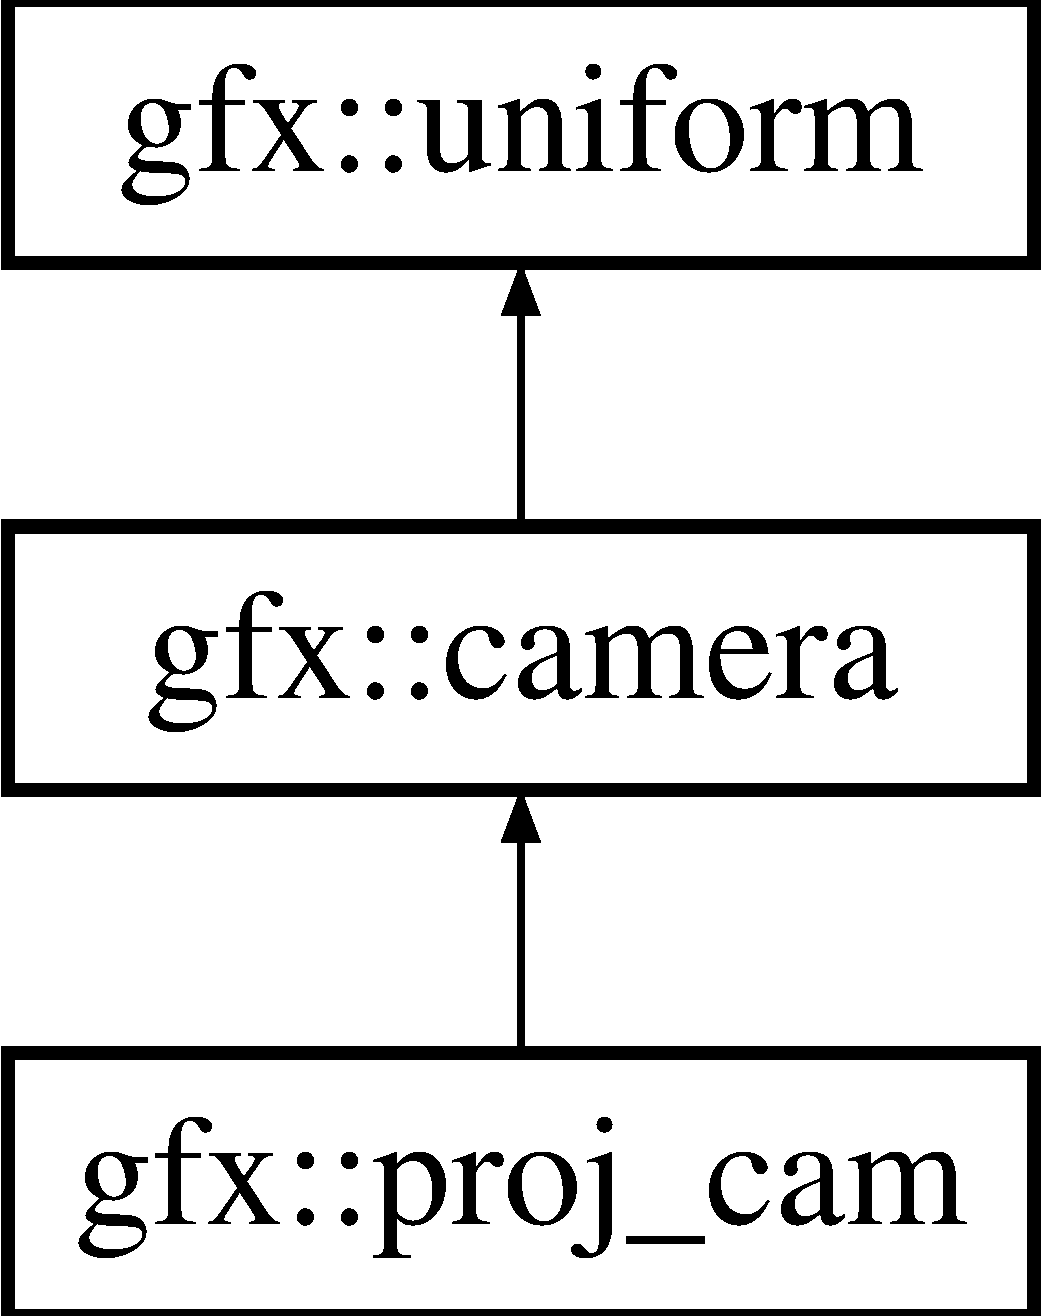
\includegraphics[height=3.000000cm]{classgfx_1_1proj__cam}
\end{center}
\end{figure}
\subsection*{Classes}
\begin{DoxyCompactItemize}
\item 
class \hyperlink{classgfx_1_1proj__cam_1_1settings}{settings}
\end{DoxyCompactItemize}
\subsection*{Public Member Functions}
\begin{DoxyCompactItemize}
\item 
\hyperlink{classgfx_1_1proj__cam_af0e3ae63279b365f1cfe9e2da5d9defc}{proj\-\_\-cam} (\hyperlink{classgfx_1_1proj__cam_1_1settings}{settings} const \&set=\hyperlink{classgfx_1_1proj__cam_1_1settings}{settings}())
\begin{DoxyCompactList}\small\item\em Construct a new projection camera. \end{DoxyCompactList}\item 
\hypertarget{classgfx_1_1proj__cam_ad82cad064ed31c060800f31783ef15f5}{\hyperlink{classgfx_1_1proj__cam_ad82cad064ed31c060800f31783ef15f5}{$\sim$proj\-\_\-cam} ()}\label{classgfx_1_1proj__cam_ad82cad064ed31c060800f31783ef15f5}

\begin{DoxyCompactList}\small\item\em Destruct this projection camera. \end{DoxyCompactList}\item 
\hyperlink{classgfx_1_1proj__cam}{proj\-\_\-cam} \& \hyperlink{classgfx_1_1proj__cam_ae4787d17c3c026fc142405ed926f5197}{position} (vec3 const \&point)
\begin{DoxyCompactList}\small\item\em Set the projection camera's position. \end{DoxyCompactList}\item 
\hyperlink{classgfx_1_1proj__cam}{proj\-\_\-cam} \& \hyperlink{classgfx_1_1proj__cam_adc330250e18123f712e295270ab82e8d}{look\-\_\-at} (vec3 const \&point)
\begin{DoxyCompactList}\small\item\em Set the point the projection camera looks at. \end{DoxyCompactList}\item 
\hyperlink{classgfx_1_1proj__cam}{proj\-\_\-cam} \& \hyperlink{classgfx_1_1proj__cam_a4a56dae9f390db460f573a128786580f}{upward} (vec3 const \&dir)
\begin{DoxyCompactList}\small\item\em Set the direction the projection camera considers to be up. \end{DoxyCompactList}\item 
\hyperlink{classgfx_1_1proj__cam}{proj\-\_\-cam} \& \hyperlink{classgfx_1_1proj__cam_ad6e333007f9a943e4fa4ffdd49d46fd7}{field\-\_\-of\-\_\-view} (d\-\_\-angle const \&vert)
\begin{DoxyCompactList}\small\item\em Set the projection camera's vertical field of view. \end{DoxyCompactList}\item 
\hyperlink{classgfx_1_1proj__cam}{proj\-\_\-cam} \& \hyperlink{classgfx_1_1proj__cam_ad8982cf936ac2ca092c428783ba4b43a}{aspect\-\_\-ratio} (double ar)
\begin{DoxyCompactList}\small\item\em Set the projection camera's aspect ratio. \end{DoxyCompactList}\item 
\hyperlink{classgfx_1_1proj__cam}{proj\-\_\-cam} \& \hyperlink{classgfx_1_1proj__cam_a43d03b8818766ea972cd0253e6207c3f}{near\-\_\-plane} (double np)
\begin{DoxyCompactList}\small\item\em Set the projection camera's near clipping plane. \end{DoxyCompactList}\item 
\hyperlink{classgfx_1_1proj__cam}{proj\-\_\-cam} \& \hyperlink{classgfx_1_1proj__cam_abc2f979a40f4467fce33b90d752cdbfa}{far\-\_\-plane} (double fp)
\begin{DoxyCompactList}\small\item\em Set the projection camera's far clipping plane. \end{DoxyCompactList}\end{DoxyCompactItemize}
\subsection*{Protected Member Functions}
\begin{DoxyCompactItemize}
\item 
\hypertarget{classgfx_1_1proj__cam_abc8a9c3bce414995385ccc7cdaeb3a1f}{virtual void \hyperlink{classgfx_1_1proj__cam_abc8a9c3bce414995385ccc7cdaeb3a1f}{update\-\_\-view} ()}\label{classgfx_1_1proj__cam_abc8a9c3bce414995385ccc7cdaeb3a1f}

\begin{DoxyCompactList}\small\item\em Update the view matrix of the projection camera. Used internally. \end{DoxyCompactList}\end{DoxyCompactItemize}
\subsection*{Protected Attributes}
\begin{DoxyCompactItemize}
\item 
\hypertarget{classgfx_1_1proj__cam_ac1ab5332debb501a37b5de30617880d2}{vec3 {\bfseries pos}}\label{classgfx_1_1proj__cam_ac1ab5332debb501a37b5de30617880d2}

\item 
\hypertarget{classgfx_1_1proj__cam_a27784dac2322e2f20e633a45a42411ab}{vec3 {\bfseries look}}\label{classgfx_1_1proj__cam_a27784dac2322e2f20e633a45a42411ab}

\item 
\hypertarget{classgfx_1_1proj__cam_a877c175c8b29f85ab3a4ea92f3e5d977}{vec3 {\bfseries up}}\label{classgfx_1_1proj__cam_a877c175c8b29f85ab3a4ea92f3e5d977}

\item 
\hypertarget{classgfx_1_1proj__cam_ac049cd3c7dbcf9cbf5b88613bed7d244}{d\-\_\-angle {\bfseries fov\-\_\-vert}}\label{classgfx_1_1proj__cam_ac049cd3c7dbcf9cbf5b88613bed7d244}

\item 
\hypertarget{classgfx_1_1proj__cam_a73fe11c5cdfe4947160bd3e7ab6b6732}{double {\bfseries aspect}}\label{classgfx_1_1proj__cam_a73fe11c5cdfe4947160bd3e7ab6b6732}

\item 
\hypertarget{classgfx_1_1proj__cam_afdbbd67b960c2ab5b9b0956cbe9030df}{double {\bfseries near}}\label{classgfx_1_1proj__cam_afdbbd67b960c2ab5b9b0956cbe9030df}

\item 
\hypertarget{classgfx_1_1proj__cam_a93986237b2dd89bf2bb47c9e676ba975}{double {\bfseries far}}\label{classgfx_1_1proj__cam_a93986237b2dd89bf2bb47c9e676ba975}

\item 
\hypertarget{classgfx_1_1proj__cam_a2f2d2e68eee3d2975056e874b05634ae}{mat4 {\bfseries perspect}}\label{classgfx_1_1proj__cam_a2f2d2e68eee3d2975056e874b05634ae}

\item 
\hypertarget{classgfx_1_1proj__cam_af3c86c7a6882a0a1b8f3820e401696f9}{bool {\bfseries proj\-\_\-changed}}\label{classgfx_1_1proj__cam_af3c86c7a6882a0a1b8f3820e401696f9}

\end{DoxyCompactItemize}


\subsection{Detailed Description}
A directable projection camera. 

Put it somewhere, tell it what to look at, and specify what up is, and it does the rest.

\begin{DoxyRefDesc}{Todo}
\item[\hyperlink{todo__todo000017}{Todo}]Ummm, chouldn't proj\-\_\-changed just be view\-\_\-changed? Review this. \end{DoxyRefDesc}


\subsection{Constructor \& Destructor Documentation}
\hypertarget{classgfx_1_1proj__cam_af0e3ae63279b365f1cfe9e2da5d9defc}{\index{gfx\-::proj\-\_\-cam@{gfx\-::proj\-\_\-cam}!proj\-\_\-cam@{proj\-\_\-cam}}
\index{proj\-\_\-cam@{proj\-\_\-cam}!gfx::proj_cam@{gfx\-::proj\-\_\-cam}}
\subsubsection[{proj\-\_\-cam}]{\setlength{\rightskip}{0pt plus 5cm}gfx\-::proj\-\_\-cam\-::proj\-\_\-cam (
\begin{DoxyParamCaption}
\item[{{\bf settings} const \&}]{set = {\ttfamily {\bf settings}()}}
\end{DoxyParamCaption}
)}}\label{classgfx_1_1proj__cam_af0e3ae63279b365f1cfe9e2da5d9defc}


Construct a new projection camera. 


\begin{DoxyParams}{Parameters}
{\em set} & The settings for the new projection camera \\
\hline
\end{DoxyParams}


\subsection{Member Function Documentation}
\hypertarget{classgfx_1_1proj__cam_ad8982cf936ac2ca092c428783ba4b43a}{\index{gfx\-::proj\-\_\-cam@{gfx\-::proj\-\_\-cam}!aspect\-\_\-ratio@{aspect\-\_\-ratio}}
\index{aspect\-\_\-ratio@{aspect\-\_\-ratio}!gfx::proj_cam@{gfx\-::proj\-\_\-cam}}
\subsubsection[{aspect\-\_\-ratio}]{\setlength{\rightskip}{0pt plus 5cm}{\bf proj\-\_\-cam} \& gfx\-::proj\-\_\-cam\-::aspect\-\_\-ratio (
\begin{DoxyParamCaption}
\item[{double}]{ar}
\end{DoxyParamCaption}
)}}\label{classgfx_1_1proj__cam_ad8982cf936ac2ca092c428783ba4b43a}


Set the projection camera's aspect ratio. 


\begin{DoxyParams}{Parameters}
{\em vert} & The aspect ratio \\
\hline
\end{DoxyParams}
\begin{DoxyReturn}{Returns}
This projection camera 
\end{DoxyReturn}
\hypertarget{classgfx_1_1proj__cam_abc2f979a40f4467fce33b90d752cdbfa}{\index{gfx\-::proj\-\_\-cam@{gfx\-::proj\-\_\-cam}!far\-\_\-plane@{far\-\_\-plane}}
\index{far\-\_\-plane@{far\-\_\-plane}!gfx::proj_cam@{gfx\-::proj\-\_\-cam}}
\subsubsection[{far\-\_\-plane}]{\setlength{\rightskip}{0pt plus 5cm}{\bf proj\-\_\-cam} \& gfx\-::proj\-\_\-cam\-::far\-\_\-plane (
\begin{DoxyParamCaption}
\item[{double}]{fp}
\end{DoxyParamCaption}
)}}\label{classgfx_1_1proj__cam_abc2f979a40f4467fce33b90d752cdbfa}


Set the projection camera's far clipping plane. 


\begin{DoxyParams}{Parameters}
{\em fp} & The distance to the far clipping plane \\
\hline
\end{DoxyParams}
\begin{DoxyReturn}{Returns}
This projection camera 
\end{DoxyReturn}
\hypertarget{classgfx_1_1proj__cam_ad6e333007f9a943e4fa4ffdd49d46fd7}{\index{gfx\-::proj\-\_\-cam@{gfx\-::proj\-\_\-cam}!field\-\_\-of\-\_\-view@{field\-\_\-of\-\_\-view}}
\index{field\-\_\-of\-\_\-view@{field\-\_\-of\-\_\-view}!gfx::proj_cam@{gfx\-::proj\-\_\-cam}}
\subsubsection[{field\-\_\-of\-\_\-view}]{\setlength{\rightskip}{0pt plus 5cm}{\bf proj\-\_\-cam} \& gfx\-::proj\-\_\-cam\-::field\-\_\-of\-\_\-view (
\begin{DoxyParamCaption}
\item[{d\-\_\-angle const \&}]{vert}
\end{DoxyParamCaption}
)}}\label{classgfx_1_1proj__cam_ad6e333007f9a943e4fa4ffdd49d46fd7}


Set the projection camera's vertical field of view. 


\begin{DoxyParams}{Parameters}
{\em vert} & The vertical field of view \\
\hline
\end{DoxyParams}
\begin{DoxyReturn}{Returns}
This projection camera 
\end{DoxyReturn}
\hypertarget{classgfx_1_1proj__cam_adc330250e18123f712e295270ab82e8d}{\index{gfx\-::proj\-\_\-cam@{gfx\-::proj\-\_\-cam}!look\-\_\-at@{look\-\_\-at}}
\index{look\-\_\-at@{look\-\_\-at}!gfx::proj_cam@{gfx\-::proj\-\_\-cam}}
\subsubsection[{look\-\_\-at}]{\setlength{\rightskip}{0pt plus 5cm}{\bf proj\-\_\-cam} \& gfx\-::proj\-\_\-cam\-::look\-\_\-at (
\begin{DoxyParamCaption}
\item[{vec3 const \&}]{point}
\end{DoxyParamCaption}
)}}\label{classgfx_1_1proj__cam_adc330250e18123f712e295270ab82e8d}


Set the point the projection camera looks at. 


\begin{DoxyParams}{Parameters}
{\em point} & The point the projection camera looks at \\
\hline
\end{DoxyParams}
\begin{DoxyReturn}{Returns}
This projection camera 
\end{DoxyReturn}
\hypertarget{classgfx_1_1proj__cam_a43d03b8818766ea972cd0253e6207c3f}{\index{gfx\-::proj\-\_\-cam@{gfx\-::proj\-\_\-cam}!near\-\_\-plane@{near\-\_\-plane}}
\index{near\-\_\-plane@{near\-\_\-plane}!gfx::proj_cam@{gfx\-::proj\-\_\-cam}}
\subsubsection[{near\-\_\-plane}]{\setlength{\rightskip}{0pt plus 5cm}{\bf proj\-\_\-cam} \& gfx\-::proj\-\_\-cam\-::near\-\_\-plane (
\begin{DoxyParamCaption}
\item[{double}]{np}
\end{DoxyParamCaption}
)}}\label{classgfx_1_1proj__cam_a43d03b8818766ea972cd0253e6207c3f}


Set the projection camera's near clipping plane. 


\begin{DoxyParams}{Parameters}
{\em np} & The distance to the near clipping plane \\
\hline
\end{DoxyParams}
\begin{DoxyReturn}{Returns}
This projection camera 
\end{DoxyReturn}
\hypertarget{classgfx_1_1proj__cam_ae4787d17c3c026fc142405ed926f5197}{\index{gfx\-::proj\-\_\-cam@{gfx\-::proj\-\_\-cam}!position@{position}}
\index{position@{position}!gfx::proj_cam@{gfx\-::proj\-\_\-cam}}
\subsubsection[{position}]{\setlength{\rightskip}{0pt plus 5cm}{\bf proj\-\_\-cam} \& gfx\-::proj\-\_\-cam\-::position (
\begin{DoxyParamCaption}
\item[{vec3 const \&}]{point}
\end{DoxyParamCaption}
)}}\label{classgfx_1_1proj__cam_ae4787d17c3c026fc142405ed926f5197}


Set the projection camera's position. 


\begin{DoxyParams}{Parameters}
{\em point} & The position of the projection camera \\
\hline
\end{DoxyParams}
\begin{DoxyReturn}{Returns}
This projection camera 
\end{DoxyReturn}
\hypertarget{classgfx_1_1proj__cam_a4a56dae9f390db460f573a128786580f}{\index{gfx\-::proj\-\_\-cam@{gfx\-::proj\-\_\-cam}!upward@{upward}}
\index{upward@{upward}!gfx::proj_cam@{gfx\-::proj\-\_\-cam}}
\subsubsection[{upward}]{\setlength{\rightskip}{0pt plus 5cm}{\bf proj\-\_\-cam} \& gfx\-::proj\-\_\-cam\-::upward (
\begin{DoxyParamCaption}
\item[{vec3 const \&}]{dir}
\end{DoxyParamCaption}
)}}\label{classgfx_1_1proj__cam_a4a56dae9f390db460f573a128786580f}


Set the direction the projection camera considers to be up. 


\begin{DoxyParams}{Parameters}
{\em dir} & The direction that the projection camera considers to be up \\
\hline
\end{DoxyParams}
\begin{DoxyReturn}{Returns}
This projection camera 
\end{DoxyReturn}


The documentation for this class was generated from the following files\-:\begin{DoxyCompactItemize}
\item 
g\-Scene/camera.\-hpp\item 
g\-Scene/camera.\-cpp\end{DoxyCompactItemize}

\hypertarget{classgfx_1_1R}{\section{gfx\-:\-:R Class Reference}
\label{classgfx_1_1R}\index{gfx\-::\-R@{gfx\-::\-R}}
}


Selects for single channel formats.  




{\ttfamily \#include \char`\"{}g\-Core/g\-Scene/texture.\-hpp\char`\"{}}

Inheritance diagram for gfx\-:\-:R\-:\begin{figure}[H]
\begin{center}
\leavevmode
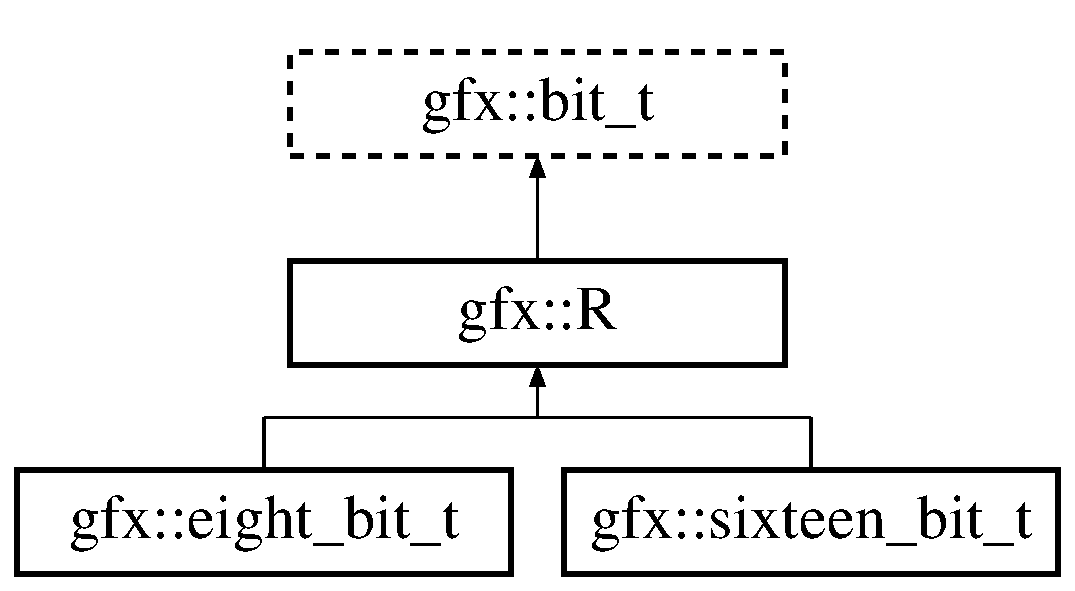
\includegraphics[height=3.000000cm]{classgfx_1_1R}
\end{center}
\end{figure}
\subsection*{Public Member Functions}
\begin{DoxyCompactItemize}
\item 
\hypertarget{classgfx_1_1R_a1ae37ad45532503dc88ec329ba938c8f}{virtual size\-\_\-t {\bfseries n} () const =0}\label{classgfx_1_1R_a1ae37ad45532503dc88ec329ba938c8f}

\end{DoxyCompactItemize}


\subsection{Detailed Description}
Selects for single channel formats. 

The documentation for this class was generated from the following file\-:\begin{DoxyCompactItemize}
\item 
g\-Scene/texture.\-hpp\end{DoxyCompactItemize}

\hypertarget{classgfx_1_1repeat__t}{\section{gfx\-:\-:repeat\-\_\-t Class Reference}
\label{classgfx_1_1repeat__t}\index{gfx\-::repeat\-\_\-t@{gfx\-::repeat\-\_\-t}}
}


Selector for repeat sampling.  




{\ttfamily \#include \char`\"{}g\-Core/g\-Video/texture.\-hpp\char`\"{}}

Inheritance diagram for gfx\-:\-:repeat\-\_\-t\-:\begin{figure}[H]
\begin{center}
\leavevmode
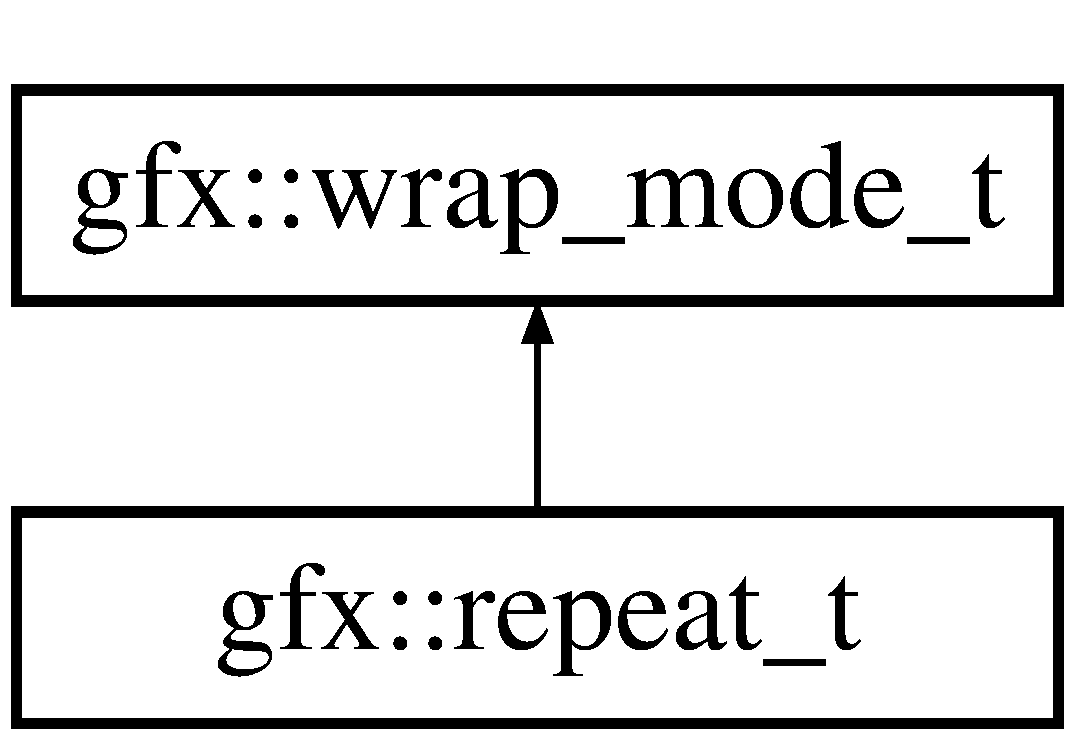
\includegraphics[height=2.000000cm]{classgfx_1_1repeat__t}
\end{center}
\end{figure}
\subsection*{Protected Member Functions}
\begin{DoxyCompactItemize}
\item 
\hypertarget{classgfx_1_1repeat__t_aba33cb8b5d640678fb7b344ad3046890}{virtual G\-Lint {\bfseries val} () const }\label{classgfx_1_1repeat__t_aba33cb8b5d640678fb7b344ad3046890}

\end{DoxyCompactItemize}
\subsection*{Friends}
\begin{DoxyCompactItemize}
\item 
\hypertarget{classgfx_1_1repeat__t_a2039d67f6166ccf823c78e3476aad9aa}{class {\bfseries texture\-\_\-1\-D}}\label{classgfx_1_1repeat__t_a2039d67f6166ccf823c78e3476aad9aa}

\item 
\hypertarget{classgfx_1_1repeat__t_a22ad86ef46c3b17357a0cd59e50bc7dd}{class {\bfseries texture\-\_\-2\-D}}\label{classgfx_1_1repeat__t_a22ad86ef46c3b17357a0cd59e50bc7dd}

\end{DoxyCompactItemize}


\subsection{Detailed Description}
Selector for repeat sampling. 

The documentation for this class was generated from the following file\-:\begin{DoxyCompactItemize}
\item 
g\-Scene/texture.\-hpp\end{DoxyCompactItemize}

\hypertarget{classgfx_1_1Rf}{\section{gfx\-:\-:Rf Class Reference}
\label{classgfx_1_1Rf}\index{gfx\-::\-Rf@{gfx\-::\-Rf}}
}


Selects for single channel floating point formats.  




{\ttfamily \#include \char`\"{}g\-Core/g\-Scene/texture.\-hpp\char`\"{}}

Inheritance diagram for gfx\-:\-:Rf\-:\begin{figure}[H]
\begin{center}
\leavevmode
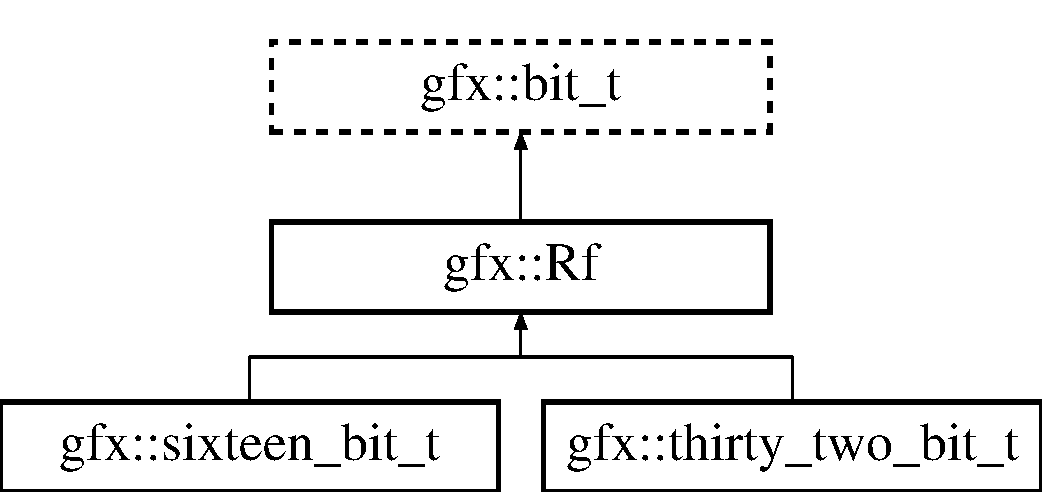
\includegraphics[height=3.000000cm]{classgfx_1_1Rf}
\end{center}
\end{figure}
\subsection*{Public Member Functions}
\begin{DoxyCompactItemize}
\item 
\hypertarget{classgfx_1_1Rf_a5fe890ef699ab5047e1c4f4e4d1ed859}{virtual size\-\_\-t {\bfseries n} () const =0}\label{classgfx_1_1Rf_a5fe890ef699ab5047e1c4f4e4d1ed859}

\end{DoxyCompactItemize}


\subsection{Detailed Description}
Selects for single channel floating point formats. 

The documentation for this class was generated from the following file\-:\begin{DoxyCompactItemize}
\item 
g\-Scene/texture.\-hpp\end{DoxyCompactItemize}

\hypertarget{classgfx_1_1RG}{\section{gfx\-:\-:R\-G Class Reference}
\label{classgfx_1_1RG}\index{gfx\-::\-R\-G@{gfx\-::\-R\-G}}
}


Selects for dual channel formats.  




{\ttfamily \#include \char`\"{}g\-Core/g\-Scene/texture.\-hpp\char`\"{}}

Inheritance diagram for gfx\-:\-:R\-G\-:\begin{figure}[H]
\begin{center}
\leavevmode
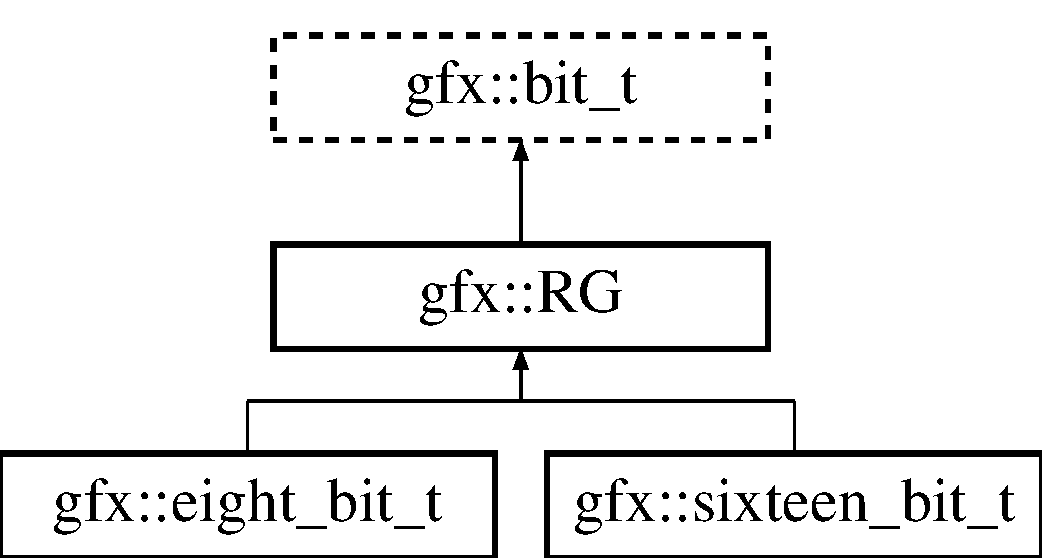
\includegraphics[height=3.000000cm]{classgfx_1_1RG}
\end{center}
\end{figure}
\subsection*{Public Member Functions}
\begin{DoxyCompactItemize}
\item 
\hypertarget{classgfx_1_1RG_a6367ebe6a7eb109c185bb894f2469df3}{virtual size\-\_\-t {\bfseries n} () const =0}\label{classgfx_1_1RG_a6367ebe6a7eb109c185bb894f2469df3}

\end{DoxyCompactItemize}


\subsection{Detailed Description}
Selects for dual channel formats. 

The documentation for this class was generated from the following file\-:\begin{DoxyCompactItemize}
\item 
g\-Scene/texture.\-hpp\end{DoxyCompactItemize}

\hypertarget{classgfx_1_1RGB}{\section{gfx\-:\-:R\-G\-B Class Reference}
\label{classgfx_1_1RGB}\index{gfx\-::\-R\-G\-B@{gfx\-::\-R\-G\-B}}
}


Selects for three channel formats.  




{\ttfamily \#include \char`\"{}g\-Core/g\-Scene/texture.\-hpp\char`\"{}}

Inheritance diagram for gfx\-:\-:R\-G\-B\-:\begin{figure}[H]
\begin{center}
\leavevmode
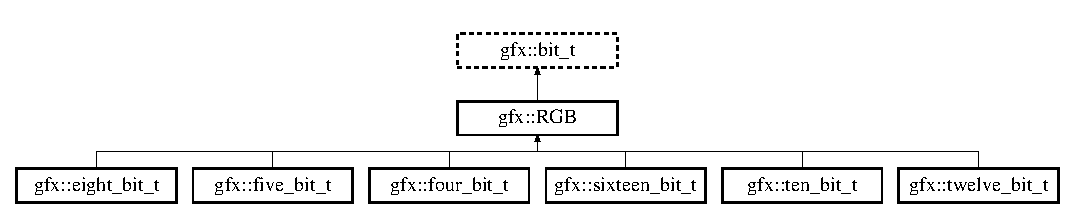
\includegraphics[height=2.500000cm]{classgfx_1_1RGB}
\end{center}
\end{figure}
\subsection*{Public Member Functions}
\begin{DoxyCompactItemize}
\item 
\hypertarget{classgfx_1_1RGB_aac0451a5d28cc5a4607086437ccb6965}{virtual size\-\_\-t {\bfseries n} () const =0}\label{classgfx_1_1RGB_aac0451a5d28cc5a4607086437ccb6965}

\end{DoxyCompactItemize}


\subsection{Detailed Description}
Selects for three channel formats. 

The documentation for this class was generated from the following file\-:\begin{DoxyCompactItemize}
\item 
g\-Scene/texture.\-hpp\end{DoxyCompactItemize}

\hypertarget{classgfx_1_1RGBA}{\section{gfx\-:\-:R\-G\-B\-A Class Reference}
\label{classgfx_1_1RGBA}\index{gfx\-::\-R\-G\-B\-A@{gfx\-::\-R\-G\-B\-A}}
}


Selects for four channel formats.  




{\ttfamily \#include \char`\"{}g\-Core/g\-Scene/texture.\-hpp\char`\"{}}

Inheritance diagram for gfx\-:\-:R\-G\-B\-A\-:\begin{figure}[H]
\begin{center}
\leavevmode
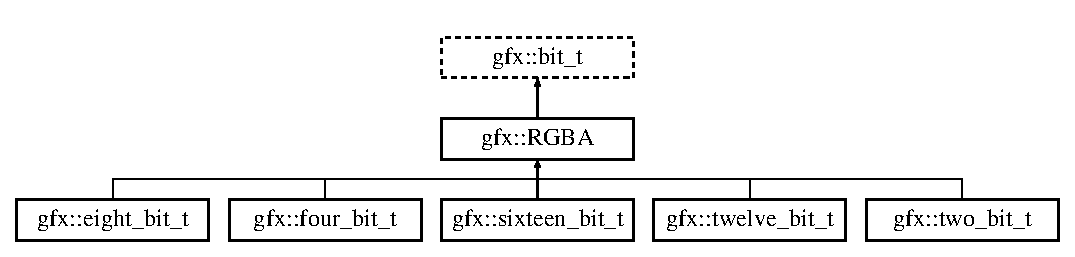
\includegraphics[height=3.000000cm]{classgfx_1_1RGBA}
\end{center}
\end{figure}
\subsection*{Public Member Functions}
\begin{DoxyCompactItemize}
\item 
\hypertarget{classgfx_1_1RGBA_a0925a6cbcc1eabedb944f880ac3ce9ea}{virtual size\-\_\-t {\bfseries n} () const =0}\label{classgfx_1_1RGBA_a0925a6cbcc1eabedb944f880ac3ce9ea}

\end{DoxyCompactItemize}


\subsection{Detailed Description}
Selects for four channel formats. 

The documentation for this class was generated from the following file\-:\begin{DoxyCompactItemize}
\item 
g\-Scene/texture.\-hpp\end{DoxyCompactItemize}

\hypertarget{classgfx_1_1RGBAf}{\section{gfx\-:\-:R\-G\-B\-Af Class Reference}
\label{classgfx_1_1RGBAf}\index{gfx\-::\-R\-G\-B\-Af@{gfx\-::\-R\-G\-B\-Af}}
}


Selects for four channel floating point formats.  




{\ttfamily \#include \char`\"{}g\-Core/g\-Scene/texture.\-hpp\char`\"{}}

Inheritance diagram for gfx\-:\-:R\-G\-B\-Af\-:\begin{figure}[H]
\begin{center}
\leavevmode
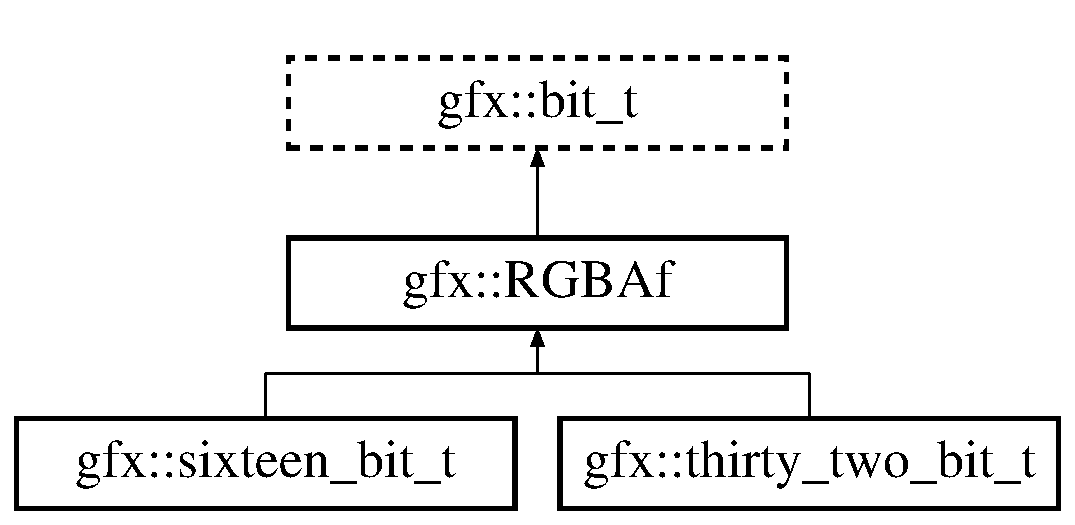
\includegraphics[height=3.000000cm]{classgfx_1_1RGBAf}
\end{center}
\end{figure}
\subsection*{Public Member Functions}
\begin{DoxyCompactItemize}
\item 
\hypertarget{classgfx_1_1RGBAf_a27e98c9c08c06b9e425dc1b0af22ad56}{virtual size\-\_\-t {\bfseries n} () const =0}\label{classgfx_1_1RGBAf_a27e98c9c08c06b9e425dc1b0af22ad56}

\end{DoxyCompactItemize}


\subsection{Detailed Description}
Selects for four channel floating point formats. 

The documentation for this class was generated from the following file\-:\begin{DoxyCompactItemize}
\item 
g\-Scene/texture.\-hpp\end{DoxyCompactItemize}

\hypertarget{classgfx_1_1RGBAi}{\section{gfx\-:\-:R\-G\-B\-Ai Class Reference}
\label{classgfx_1_1RGBAi}\index{gfx\-::\-R\-G\-B\-Ai@{gfx\-::\-R\-G\-B\-Ai}}
}


Selects for four channel integer formats.  




{\ttfamily \#include \char`\"{}g\-Core/g\-Scene/texture.\-hpp\char`\"{}}

Inheritance diagram for gfx\-:\-:R\-G\-B\-Ai\-:\begin{figure}[H]
\begin{center}
\leavevmode
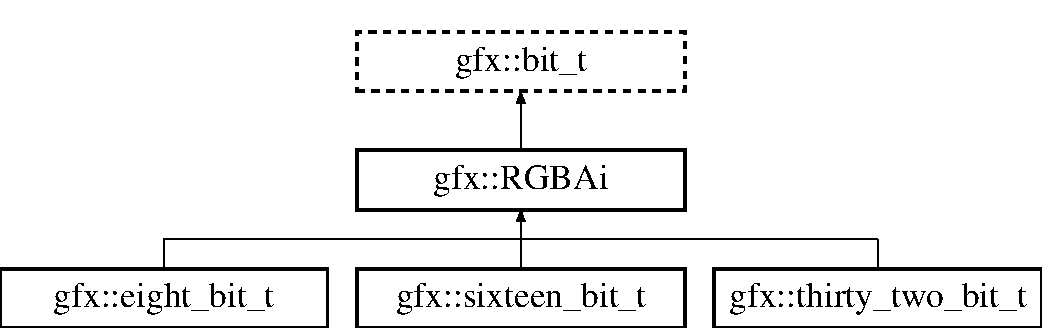
\includegraphics[height=3.000000cm]{classgfx_1_1RGBAi}
\end{center}
\end{figure}
\subsection*{Public Member Functions}
\begin{DoxyCompactItemize}
\item 
\hypertarget{classgfx_1_1RGBAi_a9540c83f0596401fda7acffbe0badb76}{virtual size\-\_\-t {\bfseries n} () const =0}\label{classgfx_1_1RGBAi_a9540c83f0596401fda7acffbe0badb76}

\end{DoxyCompactItemize}


\subsection{Detailed Description}
Selects for four channel integer formats. 

The documentation for this class was generated from the following file\-:\begin{DoxyCompactItemize}
\item 
g\-Scene/texture.\-hpp\end{DoxyCompactItemize}

\hypertarget{classgfx_1_1RGBAsn}{\section{gfx\-:\-:R\-G\-B\-Asn Class Reference}
\label{classgfx_1_1RGBAsn}\index{gfx\-::\-R\-G\-B\-Asn@{gfx\-::\-R\-G\-B\-Asn}}
}


Selects for four channel signed integer formats.  




{\ttfamily \#include \char`\"{}g\-Core/g\-Scene/texture.\-hpp\char`\"{}}

Inheritance diagram for gfx\-:\-:R\-G\-B\-Asn\-:\begin{figure}[H]
\begin{center}
\leavevmode
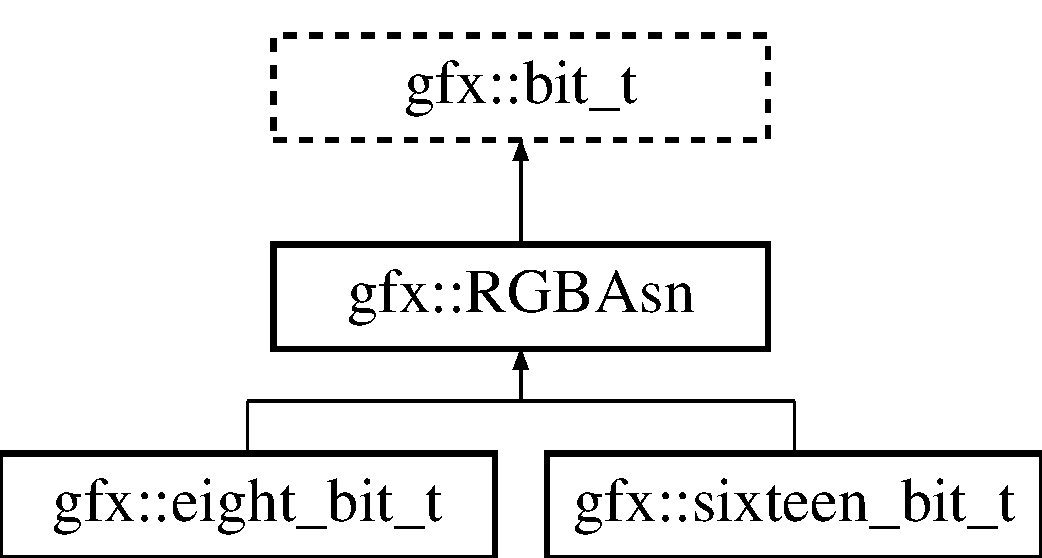
\includegraphics[height=3.000000cm]{classgfx_1_1RGBAsn}
\end{center}
\end{figure}
\subsection*{Public Member Functions}
\begin{DoxyCompactItemize}
\item 
\hypertarget{classgfx_1_1RGBAsn_ae38a51cd1ae1705fb3ad291240b6fff5}{virtual size\-\_\-t {\bfseries n} () const =0}\label{classgfx_1_1RGBAsn_ae38a51cd1ae1705fb3ad291240b6fff5}

\end{DoxyCompactItemize}


\subsection{Detailed Description}
Selects for four channel signed integer formats. 

The documentation for this class was generated from the following file\-:\begin{DoxyCompactItemize}
\item 
g\-Scene/texture.\-hpp\end{DoxyCompactItemize}

\hypertarget{classgfx_1_1RGBAui}{\section{gfx\-:\-:R\-G\-B\-Aui Class Reference}
\label{classgfx_1_1RGBAui}\index{gfx\-::\-R\-G\-B\-Aui@{gfx\-::\-R\-G\-B\-Aui}}
}


Selects for four channel unsigned integer formats.  




{\ttfamily \#include \char`\"{}g\-Core/g\-Scene/texture.\-hpp\char`\"{}}

Inheritance diagram for gfx\-:\-:R\-G\-B\-Aui\-:\begin{figure}[H]
\begin{center}
\leavevmode
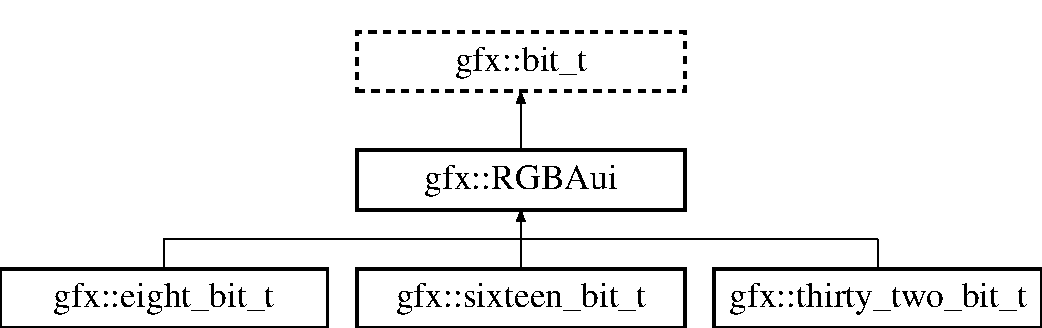
\includegraphics[height=3.000000cm]{classgfx_1_1RGBAui}
\end{center}
\end{figure}
\subsection*{Public Member Functions}
\begin{DoxyCompactItemize}
\item 
\hypertarget{classgfx_1_1RGBAui_aabd6223ecdcc6b4f2b9ee1fa5b4d6b58}{virtual size\-\_\-t {\bfseries n} () const =0}\label{classgfx_1_1RGBAui_aabd6223ecdcc6b4f2b9ee1fa5b4d6b58}

\end{DoxyCompactItemize}


\subsection{Detailed Description}
Selects for four channel unsigned integer formats. 

The documentation for this class was generated from the following file\-:\begin{DoxyCompactItemize}
\item 
g\-Scene/texture.\-hpp\end{DoxyCompactItemize}

\hypertarget{classgfx_1_1RGBf}{\section{gfx\-:\-:R\-G\-Bf Class Reference}
\label{classgfx_1_1RGBf}\index{gfx\-::\-R\-G\-Bf@{gfx\-::\-R\-G\-Bf}}
}


Selects for four channel floating point formats.  




{\ttfamily \#include \char`\"{}g\-Core/g\-Scene/texture.\-hpp\char`\"{}}

Inheritance diagram for gfx\-:\-:R\-G\-Bf\-:\begin{figure}[H]
\begin{center}
\leavevmode
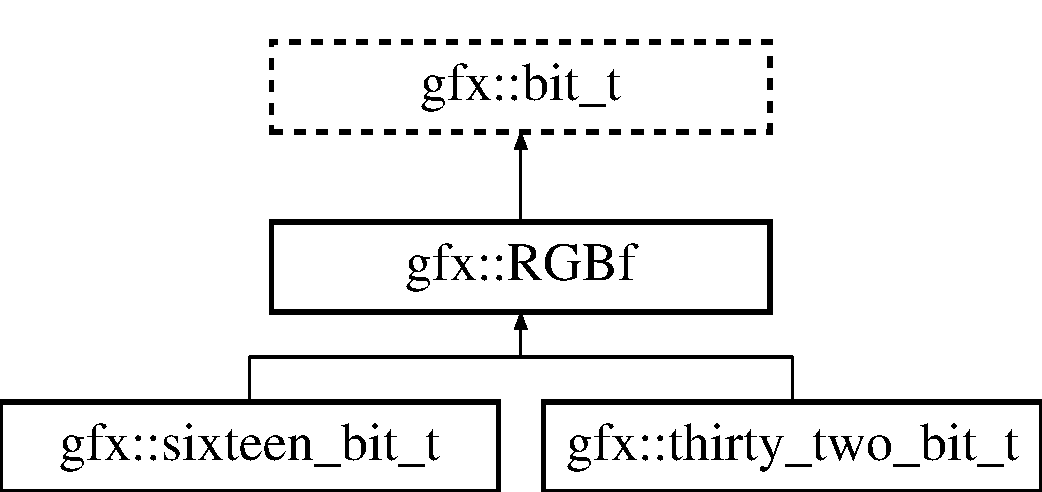
\includegraphics[height=3.000000cm]{classgfx_1_1RGBf}
\end{center}
\end{figure}
\subsection*{Public Member Functions}
\begin{DoxyCompactItemize}
\item 
\hypertarget{classgfx_1_1RGBf_ad6992f7733a45fbaf2d90864065fd97a}{virtual size\-\_\-t {\bfseries n} () const =0}\label{classgfx_1_1RGBf_ad6992f7733a45fbaf2d90864065fd97a}

\end{DoxyCompactItemize}


\subsection{Detailed Description}
Selects for four channel floating point formats. 

The documentation for this class was generated from the following file\-:\begin{DoxyCompactItemize}
\item 
g\-Scene/texture.\-hpp\end{DoxyCompactItemize}

\hypertarget{classgfx_1_1RGBi}{\section{gfx\-:\-:R\-G\-Bi Class Reference}
\label{classgfx_1_1RGBi}\index{gfx\-::\-R\-G\-Bi@{gfx\-::\-R\-G\-Bi}}
}


Selects for four channel integer formats.  




{\ttfamily \#include \char`\"{}g\-Core/g\-Scene/texture.\-hpp\char`\"{}}

Inheritance diagram for gfx\-:\-:R\-G\-Bi\-:\begin{figure}[H]
\begin{center}
\leavevmode
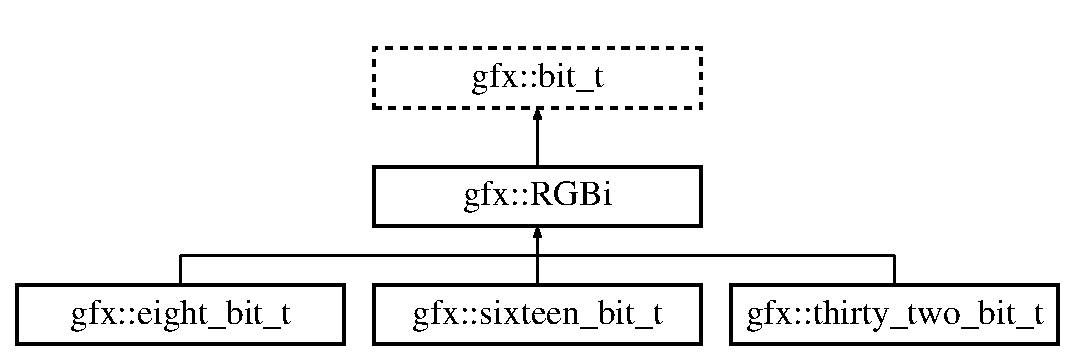
\includegraphics[height=3.000000cm]{classgfx_1_1RGBi}
\end{center}
\end{figure}
\subsection*{Public Member Functions}
\begin{DoxyCompactItemize}
\item 
\hypertarget{classgfx_1_1RGBi_a0e5d42e77bed28e5148e8c3f371ea562}{virtual size\-\_\-t {\bfseries n} () const =0}\label{classgfx_1_1RGBi_a0e5d42e77bed28e5148e8c3f371ea562}

\end{DoxyCompactItemize}


\subsection{Detailed Description}
Selects for four channel integer formats. 

The documentation for this class was generated from the following file\-:\begin{DoxyCompactItemize}
\item 
g\-Scene/texture.\-hpp\end{DoxyCompactItemize}

\hypertarget{classgfx_1_1RGBsn}{\section{gfx\-:\-:R\-G\-Bsn Class Reference}
\label{classgfx_1_1RGBsn}\index{gfx\-::\-R\-G\-Bsn@{gfx\-::\-R\-G\-Bsn}}
}


Selects for four channel signed integer formats.  




{\ttfamily \#include \char`\"{}g\-Core/g\-Scene/texture.\-hpp\char`\"{}}

Inheritance diagram for gfx\-:\-:R\-G\-Bsn\-:\begin{figure}[H]
\begin{center}
\leavevmode
\includegraphics[height=3.000000cm]{classgfx_1_1RGBsn}
\end{center}
\end{figure}
\subsection*{Public Member Functions}
\begin{DoxyCompactItemize}
\item 
\hypertarget{classgfx_1_1RGBsn_aca578d4da90ea5d67f9ac05bee2d7a93}{virtual size\-\_\-t {\bfseries n} () const =0}\label{classgfx_1_1RGBsn_aca578d4da90ea5d67f9ac05bee2d7a93}

\end{DoxyCompactItemize}


\subsection{Detailed Description}
Selects for four channel signed integer formats. 

The documentation for this class was generated from the following file\-:\begin{DoxyCompactItemize}
\item 
g\-Scene/texture.\-hpp\end{DoxyCompactItemize}

\hypertarget{classgfx_1_1RGBui}{\section{gfx\-:\-:R\-G\-Bui Class Reference}
\label{classgfx_1_1RGBui}\index{gfx\-::\-R\-G\-Bui@{gfx\-::\-R\-G\-Bui}}
}


Selects for four channel unsigned integer formats.  




{\ttfamily \#include \char`\"{}g\-Core/g\-Scene/texture.\-hpp\char`\"{}}

Inheritance diagram for gfx\-:\-:R\-G\-Bui\-:\begin{figure}[H]
\begin{center}
\leavevmode
\includegraphics[height=3.000000cm]{classgfx_1_1RGBui}
\end{center}
\end{figure}
\subsection*{Public Member Functions}
\begin{DoxyCompactItemize}
\item 
\hypertarget{classgfx_1_1RGBui_a7c9ef4a292cb08ee81a0cf4d32acb14c}{virtual size\-\_\-t {\bfseries n} () const =0}\label{classgfx_1_1RGBui_a7c9ef4a292cb08ee81a0cf4d32acb14c}

\end{DoxyCompactItemize}


\subsection{Detailed Description}
Selects for four channel unsigned integer formats. 

The documentation for this class was generated from the following file\-:\begin{DoxyCompactItemize}
\item 
g\-Scene/texture.\-hpp\end{DoxyCompactItemize}

\hypertarget{classgfx_1_1RGf}{\section{gfx\-:\-:R\-Gf Class Reference}
\label{classgfx_1_1RGf}\index{gfx\-::\-R\-Gf@{gfx\-::\-R\-Gf}}
}


Selects for dual channel floating point formats.  




{\ttfamily \#include \char`\"{}g\-Core/g\-Scene/texture.\-hpp\char`\"{}}

Inheritance diagram for gfx\-:\-:R\-Gf\-:\begin{figure}[H]
\begin{center}
\leavevmode
\includegraphics[height=3.000000cm]{classgfx_1_1RGf}
\end{center}
\end{figure}
\subsection*{Public Member Functions}
\begin{DoxyCompactItemize}
\item 
\hypertarget{classgfx_1_1RGf_a24e5102b767a74ccb5efcf164ba1ccb1}{virtual size\-\_\-t {\bfseries n} () const =0}\label{classgfx_1_1RGf_a24e5102b767a74ccb5efcf164ba1ccb1}

\end{DoxyCompactItemize}


\subsection{Detailed Description}
Selects for dual channel floating point formats. 

The documentation for this class was generated from the following file\-:\begin{DoxyCompactItemize}
\item 
g\-Scene/texture.\-hpp\end{DoxyCompactItemize}

\hypertarget{classgfx_1_1RGi}{\section{gfx\-:\-:R\-Gi Class Reference}
\label{classgfx_1_1RGi}\index{gfx\-::\-R\-Gi@{gfx\-::\-R\-Gi}}
}


Selects for dual channel integer formats.  




{\ttfamily \#include \char`\"{}g\-Core/g\-Scene/texture.\-hpp\char`\"{}}

Inheritance diagram for gfx\-:\-:R\-Gi\-:\begin{figure}[H]
\begin{center}
\leavevmode
\includegraphics[height=3.000000cm]{classgfx_1_1RGi}
\end{center}
\end{figure}
\subsection*{Public Member Functions}
\begin{DoxyCompactItemize}
\item 
\hypertarget{classgfx_1_1RGi_ab0e559f567589dd6516d13930f7d172f}{virtual size\-\_\-t {\bfseries n} () const =0}\label{classgfx_1_1RGi_ab0e559f567589dd6516d13930f7d172f}

\end{DoxyCompactItemize}


\subsection{Detailed Description}
Selects for dual channel integer formats. 

The documentation for this class was generated from the following file\-:\begin{DoxyCompactItemize}
\item 
g\-Scene/texture.\-hpp\end{DoxyCompactItemize}

\hypertarget{classgfx_1_1RGsn}{\section{gfx\-:\-:R\-Gsn Class Reference}
\label{classgfx_1_1RGsn}\index{gfx\-::\-R\-Gsn@{gfx\-::\-R\-Gsn}}
}


Selects for dual channel signed integer formats.  




{\ttfamily \#include \char`\"{}g\-Core/g\-Scene/texture.\-hpp\char`\"{}}

Inheritance diagram for gfx\-:\-:R\-Gsn\-:\begin{figure}[H]
\begin{center}
\leavevmode
\includegraphics[height=3.000000cm]{classgfx_1_1RGsn}
\end{center}
\end{figure}
\subsection*{Public Member Functions}
\begin{DoxyCompactItemize}
\item 
\hypertarget{classgfx_1_1RGsn_a37696bc2a0a48aaf43fa477d9563c1f0}{virtual size\-\_\-t {\bfseries n} () const =0}\label{classgfx_1_1RGsn_a37696bc2a0a48aaf43fa477d9563c1f0}

\end{DoxyCompactItemize}


\subsection{Detailed Description}
Selects for dual channel signed integer formats. 

The documentation for this class was generated from the following file\-:\begin{DoxyCompactItemize}
\item 
g\-Scene/texture.\-hpp\end{DoxyCompactItemize}

\hypertarget{classgfx_1_1RGui}{\section{gfx\-:\-:R\-Gui Class Reference}
\label{classgfx_1_1RGui}\index{gfx\-::\-R\-Gui@{gfx\-::\-R\-Gui}}
}


Selects for dual channel unsigned integer formats.  




{\ttfamily \#include \char`\"{}g\-Core/g\-Scene/texture.\-hpp\char`\"{}}

Inheritance diagram for gfx\-:\-:R\-Gui\-:\begin{figure}[H]
\begin{center}
\leavevmode
\includegraphics[height=3.000000cm]{classgfx_1_1RGui}
\end{center}
\end{figure}
\subsection*{Public Member Functions}
\begin{DoxyCompactItemize}
\item 
\hypertarget{classgfx_1_1RGui_af80bb91ee2f476a3d7d47276e19f7ffa}{virtual size\-\_\-t {\bfseries n} () const =0}\label{classgfx_1_1RGui_af80bb91ee2f476a3d7d47276e19f7ffa}

\end{DoxyCompactItemize}


\subsection{Detailed Description}
Selects for dual channel unsigned integer formats. 

The documentation for this class was generated from the following file\-:\begin{DoxyCompactItemize}
\item 
g\-Scene/texture.\-hpp\end{DoxyCompactItemize}

\hypertarget{classgfx_1_1Ri}{\section{gfx\-:\-:Ri Class Reference}
\label{classgfx_1_1Ri}\index{gfx\-::\-Ri@{gfx\-::\-Ri}}
}


Selects for single channel integer formats.  




{\ttfamily \#include \char`\"{}g\-Core/g\-Scene/texture.\-hpp\char`\"{}}

Inheritance diagram for gfx\-:\-:Ri\-:\begin{figure}[H]
\begin{center}
\leavevmode
\includegraphics[height=3.000000cm]{classgfx_1_1Ri}
\end{center}
\end{figure}
\subsection*{Public Member Functions}
\begin{DoxyCompactItemize}
\item 
\hypertarget{classgfx_1_1Ri_a7c8820a50a664d7cb2bd28606943897d}{virtual size\-\_\-t {\bfseries n} () const =0}\label{classgfx_1_1Ri_a7c8820a50a664d7cb2bd28606943897d}

\end{DoxyCompactItemize}


\subsection{Detailed Description}
Selects for single channel integer formats. 

The documentation for this class was generated from the following file\-:\begin{DoxyCompactItemize}
\item 
g\-Scene/texture.\-hpp\end{DoxyCompactItemize}

\hypertarget{classgfx_1_1Rsn}{\section{gfx\-:\-:Rsn Class Reference}
\label{classgfx_1_1Rsn}\index{gfx\-::\-Rsn@{gfx\-::\-Rsn}}
}


Selects for single channel signed integer formats.  




{\ttfamily \#include \char`\"{}g\-Core/g\-Scene/texture.\-hpp\char`\"{}}

Inheritance diagram for gfx\-:\-:Rsn\-:\begin{figure}[H]
\begin{center}
\leavevmode
\includegraphics[height=3.000000cm]{classgfx_1_1Rsn}
\end{center}
\end{figure}
\subsection*{Public Member Functions}
\begin{DoxyCompactItemize}
\item 
\hypertarget{classgfx_1_1Rsn_ad82b30257dd6df635e7d2c985974a2c7}{virtual size\-\_\-t {\bfseries n} () const =0}\label{classgfx_1_1Rsn_ad82b30257dd6df635e7d2c985974a2c7}

\end{DoxyCompactItemize}


\subsection{Detailed Description}
Selects for single channel signed integer formats. 

The documentation for this class was generated from the following file\-:\begin{DoxyCompactItemize}
\item 
g\-Scene/texture.\-hpp\end{DoxyCompactItemize}

\hypertarget{classgfx_1_1Rui}{\section{gfx\-:\-:Rui Class Reference}
\label{classgfx_1_1Rui}\index{gfx\-::\-Rui@{gfx\-::\-Rui}}
}


Selects for single channel unsigned integer formats.  




{\ttfamily \#include \char`\"{}g\-Core/g\-Scene/texture.\-hpp\char`\"{}}

Inheritance diagram for gfx\-:\-:Rui\-:\begin{figure}[H]
\begin{center}
\leavevmode
\includegraphics[height=3.000000cm]{classgfx_1_1Rui}
\end{center}
\end{figure}
\subsection*{Public Member Functions}
\begin{DoxyCompactItemize}
\item 
\hypertarget{classgfx_1_1Rui_a349e5306cdc4abc1c0117ac3a4725440}{virtual size\-\_\-t {\bfseries n} () const =0}\label{classgfx_1_1Rui_a349e5306cdc4abc1c0117ac3a4725440}

\end{DoxyCompactItemize}


\subsection{Detailed Description}
Selects for single channel unsigned integer formats. 

The documentation for this class was generated from the following file\-:\begin{DoxyCompactItemize}
\item 
g\-Scene/texture.\-hpp\end{DoxyCompactItemize}

\hypertarget{classgfx_1_1window_1_1setings__3D}{\section{gfx\-:\-:window\-:\-:setings\-\_\-3\-D Class Reference}
\label{classgfx_1_1window_1_1setings__3D}\index{gfx\-::window\-::setings\-\_\-3\-D@{gfx\-::window\-::setings\-\_\-3\-D}}
}


A settings object for \hyperlink{classgfx_1_1window}{windows} conerned with 3\-D rendering settings.  




{\ttfamily \#include \char`\"{}g\-Core/g\-Video/window.\-hpp\char`\"{}}



\subsection{Detailed Description}
A settings object for \hyperlink{classgfx_1_1window}{windows} conerned with 3\-D rendering settings. 

Distinct from \hyperlink{classgfx_1_1window_1_1settings}{settings}, \hyperlink{classgfx_1_1window_1_1settings__3D}{settings\-\_\-3\-D} keeps the Open\-G\-L relevent settings separate. This may be useful in some use cases, such as parsing high level graphical setting data in an application and not wanting to drag around the regular settings object in the process. \begin{DoxySeeAlso}{See Also}
\hyperlink{classgfx_1_1window}{gfx\-::window} 

\hyperlink{classgfx_1_1window_1_1settings}{gfx\-::window\-::settings} 
\end{DoxySeeAlso}


The documentation for this class was generated from the following file\-:\begin{DoxyCompactItemize}
\item 
g\-Video/window.\-hpp\end{DoxyCompactItemize}

\hypertarget{classgfx_1_1video__system_1_1settings}{\section{gfx\-:\-:video\-\_\-system\-:\-:settings Class Reference}
\label{classgfx_1_1video__system_1_1settings}\index{gfx\-::video\-\_\-system\-::settings@{gfx\-::video\-\_\-system\-::settings}}
}


Configuration class for \hyperlink{classgfx_1_1video__system}{video\-\_\-system}.  




{\ttfamily \#include \char`\"{}g\-Core/g\-Video/video\-\_\-system.\-hpp\char`\"{}}

\subsection*{Public Member Functions}
\begin{DoxyCompactItemize}
\item 
\hyperlink{classgfx_1_1video__system_1_1settings_a62b87a967d92b32dfe5fa3b2d7e62a64}{settings} ()
\begin{DoxyCompactList}\small\item\em Construct a \hyperlink{classgfx_1_1video__system_1_1settings}{settings} object with default values. \end{DoxyCompactList}\item 
\hyperlink{classgfx_1_1video__system_1_1settings}{settings} \& \hyperlink{classgfx_1_1video__system_1_1settings_a10aa8cb5d2c7cccd100b9740dd61690c}{maj\-\_\-ver} (unsigned int maj\-\_\-ver)
\begin{DoxyCompactList}\small\item\em Set the Open\-G\-L major version to the given value. \end{DoxyCompactList}\item 
\hyperlink{classgfx_1_1video__system_1_1settings}{settings} \& \hyperlink{classgfx_1_1video__system_1_1settings_aab74f7109a3e20e721736895aacd8f7a}{min\-\_\-ver} (unsigned int min\-\_\-ver)
\begin{DoxyCompactList}\small\item\em Set the Open\-G\-L minor version to the given value. \end{DoxyCompactList}\item 
\hyperlink{classgfx_1_1video__system_1_1settings}{settings} \& \hyperlink{classgfx_1_1video__system_1_1settings_afba6ac346d6b69677560ffc67b8da969}{sub\-\_\-ver} (unsigned int sub\-\_\-ver)
\begin{DoxyCompactList}\small\item\em Set the Open\-G\-L subversion to the given value. \end{DoxyCompactList}\item 
\hyperlink{classgfx_1_1video__system_1_1settings}{settings} \& \hyperlink{classgfx_1_1video__system_1_1settings_a51fa05bb7b557620bc5674e1c08bd440}{ver} (unsigned int \hyperlink{classgfx_1_1video__system_1_1settings_a10aa8cb5d2c7cccd100b9740dd61690c}{maj\-\_\-ver}, unsigned int \hyperlink{classgfx_1_1video__system_1_1settings_aab74f7109a3e20e721736895aacd8f7a}{min\-\_\-ver}, unsigned int \hyperlink{classgfx_1_1video__system_1_1settings_afba6ac346d6b69677560ffc67b8da969}{sub\-\_\-ver}=0)
\begin{DoxyCompactList}\small\item\em Set the Open\-G\-L version to the given values. \end{DoxyCompactList}\item 
\hyperlink{classgfx_1_1video__system_1_1settings}{settings} \& \hyperlink{classgfx_1_1video__system_1_1settings_add121587f4a6510390ec102fdb6f1d82}{ver} (\hyperlink{classgfx_1_1version}{version} const \&ver)
\begin{DoxyCompactList}\small\item\em Set the Open\-G\-L version to the given values. \end{DoxyCompactList}\item 
\hyperlink{classgfx_1_1video__system_1_1settings}{settings} \& \hyperlink{classgfx_1_1video__system_1_1settings_a8eb561a87de6c5268aeea6ad0c942a7a}{core\-\_\-profile} ()
\begin{DoxyCompactList}\small\item\em Set the video system to use the core Open\-G\-L profile. \end{DoxyCompactList}\item 
\hyperlink{classgfx_1_1video__system_1_1settings}{settings} \& \hyperlink{classgfx_1_1video__system_1_1settings_a5f8cdce3920df80ff413976b5ce74da1}{compatibility\-\_\-profile} ()
\begin{DoxyCompactList}\small\item\em Set the video system to use the compatibility Open\-G\-L profile. \end{DoxyCompactList}\item 
\hyperlink{classgfx_1_1video__system_1_1settings}{settings} \& \hyperlink{classgfx_1_1video__system_1_1settings_a2a7f92421494055d3a88f4151276bfe6}{es\-\_\-profile} ()
\begin{DoxyCompactList}\small\item\em Set the video system to use the E\-S Open\-G\-L profile. \end{DoxyCompactList}\end{DoxyCompactItemize}
\subsection*{Friends}
\begin{DoxyCompactItemize}
\item 
\hypertarget{classgfx_1_1video__system_1_1settings_abfd69a86b028655cf7807981b1c58526}{class {\bfseries video\-\_\-system}}\label{classgfx_1_1video__system_1_1settings_abfd69a86b028655cf7807981b1c58526}

\end{DoxyCompactItemize}


\subsection{Detailed Description}
Configuration class for \hyperlink{classgfx_1_1video__system}{video\-\_\-system}. 

The settings member of \hyperlink{classgfx_1_1video__system}{video\-\_\-system} is a public interface for configuring the video system when it is initialized. It's mutator member functions can be chained; subsequent calls to these functions overwrite changes created by previous calls. 

\subsection{Constructor \& Destructor Documentation}
\hypertarget{classgfx_1_1video__system_1_1settings_a62b87a967d92b32dfe5fa3b2d7e62a64}{\index{gfx\-::video\-\_\-system\-::settings@{gfx\-::video\-\_\-system\-::settings}!settings@{settings}}
\index{settings@{settings}!gfx::video_system::settings@{gfx\-::video\-\_\-system\-::settings}}
\subsubsection[{settings}]{\setlength{\rightskip}{0pt plus 5cm}gfx\-::video\-\_\-system\-::settings\-::settings (
\begin{DoxyParamCaption}
{}
\end{DoxyParamCaption}
)\hspace{0.3cm}{\ttfamily [inline]}}}\label{classgfx_1_1video__system_1_1settings_a62b87a967d92b32dfe5fa3b2d7e62a64}


Construct a \hyperlink{classgfx_1_1video__system_1_1settings}{settings} object with default values. 

The default settings for the \hyperlink{classgfx_1_1video__system}{gfx\-:\-:video system} are to use Open\-G\-L 1.\-4 with the core profile. 

\subsection{Member Function Documentation}
\hypertarget{classgfx_1_1video__system_1_1settings_a5f8cdce3920df80ff413976b5ce74da1}{\index{gfx\-::video\-\_\-system\-::settings@{gfx\-::video\-\_\-system\-::settings}!compatibility\-\_\-profile@{compatibility\-\_\-profile}}
\index{compatibility\-\_\-profile@{compatibility\-\_\-profile}!gfx::video_system::settings@{gfx\-::video\-\_\-system\-::settings}}
\subsubsection[{compatibility\-\_\-profile}]{\setlength{\rightskip}{0pt plus 5cm}{\bf video\-\_\-system\-::settings} \& gfx\-::video\-\_\-system\-::settings\-::compatibility\-\_\-profile (
\begin{DoxyParamCaption}
{}
\end{DoxyParamCaption}
)\hspace{0.3cm}{\ttfamily [inline]}}}\label{classgfx_1_1video__system_1_1settings_a5f8cdce3920df80ff413976b5ce74da1}


Set the video system to use the compatibility Open\-G\-L profile. 

The compatibility Open\-G\-L profile is the profile associated with the functionality for the given Open\-G\-L version and any deprecated or removed functionality; versions after 2.\-0 will provide the \hyperlink{classgfx_1_1program}{shader} pipeline but still have the old drawing functions available for use. \begin{DoxyReturn}{Returns}
This settings object 
\end{DoxyReturn}
\begin{DoxySeeAlso}{See Also}
\hyperlink{classgfx_1_1video__system_1_1settings_a8eb561a87de6c5268aeea6ad0c942a7a}{gfx\-::video\-\_\-system\-::settings\-::core\-\_\-profile()} 

\hyperlink{classgfx_1_1video__system_1_1settings_a2a7f92421494055d3a88f4151276bfe6}{gfx\-::video\-\_\-system\-::settings\-::es\-\_\-profile()} 
\end{DoxySeeAlso}
\hypertarget{classgfx_1_1video__system_1_1settings_a8eb561a87de6c5268aeea6ad0c942a7a}{\index{gfx\-::video\-\_\-system\-::settings@{gfx\-::video\-\_\-system\-::settings}!core\-\_\-profile@{core\-\_\-profile}}
\index{core\-\_\-profile@{core\-\_\-profile}!gfx::video_system::settings@{gfx\-::video\-\_\-system\-::settings}}
\subsubsection[{core\-\_\-profile}]{\setlength{\rightskip}{0pt plus 5cm}{\bf video\-\_\-system\-::settings} \& gfx\-::video\-\_\-system\-::settings\-::core\-\_\-profile (
\begin{DoxyParamCaption}
{}
\end{DoxyParamCaption}
)\hspace{0.3cm}{\ttfamily [inline]}}}\label{classgfx_1_1video__system_1_1settings_a8eb561a87de6c5268aeea6ad0c942a7a}


Set the video system to use the core Open\-G\-L profile. 

The core Open\-G\-L profile is the profile associated with the core functionality for the given Open\-G\-L version; for versions after 2.\-0 this means that the old drawing functions are depracted and not available for use and instead the \hyperlink{classgfx_1_1program}{shader} pipeline should be used. \begin{DoxyReturn}{Returns}
This settings object 
\end{DoxyReturn}
\begin{DoxySeeAlso}{See Also}
\hyperlink{classgfx_1_1video__system_1_1settings_a5f8cdce3920df80ff413976b5ce74da1}{gfx\-::video\-\_\-system\-::settings\-::compatibility\-\_\-profile()} 

\hyperlink{classgfx_1_1video__system_1_1settings_a2a7f92421494055d3a88f4151276bfe6}{gfx\-::video\-\_\-system\-::settings\-::es\-\_\-profile()} 
\end{DoxySeeAlso}
\hypertarget{classgfx_1_1video__system_1_1settings_a2a7f92421494055d3a88f4151276bfe6}{\index{gfx\-::video\-\_\-system\-::settings@{gfx\-::video\-\_\-system\-::settings}!es\-\_\-profile@{es\-\_\-profile}}
\index{es\-\_\-profile@{es\-\_\-profile}!gfx::video_system::settings@{gfx\-::video\-\_\-system\-::settings}}
\subsubsection[{es\-\_\-profile}]{\setlength{\rightskip}{0pt plus 5cm}{\bf video\-\_\-system\-::settings} \& gfx\-::video\-\_\-system\-::settings\-::es\-\_\-profile (
\begin{DoxyParamCaption}
{}
\end{DoxyParamCaption}
)\hspace{0.3cm}{\ttfamily [inline]}}}\label{classgfx_1_1video__system_1_1settings_a2a7f92421494055d3a88f4151276bfe6}


Set the video system to use the E\-S Open\-G\-L profile. 

The E\-S Open\-G\-L profile is the profile associated with mobile development. Check Open\-G\-L documention for details on what functionality is available. \begin{DoxyReturn}{Returns}
This settings object 
\end{DoxyReturn}
\begin{DoxySeeAlso}{See Also}
\hyperlink{classgfx_1_1video__system_1_1settings_a8eb561a87de6c5268aeea6ad0c942a7a}{gfx\-::video\-\_\-system\-::settings\-::core\-\_\-profile()} 

\hyperlink{classgfx_1_1video__system_1_1settings_a5f8cdce3920df80ff413976b5ce74da1}{gfx\-::video\-\_\-system\-::settings\-::compatibility\-\_\-profile()} 
\end{DoxySeeAlso}
\hypertarget{classgfx_1_1video__system_1_1settings_a10aa8cb5d2c7cccd100b9740dd61690c}{\index{gfx\-::video\-\_\-system\-::settings@{gfx\-::video\-\_\-system\-::settings}!maj\-\_\-ver@{maj\-\_\-ver}}
\index{maj\-\_\-ver@{maj\-\_\-ver}!gfx::video_system::settings@{gfx\-::video\-\_\-system\-::settings}}
\subsubsection[{maj\-\_\-ver}]{\setlength{\rightskip}{0pt plus 5cm}{\bf video\-\_\-system\-::settings} \& gfx\-::video\-\_\-system\-::settings\-::maj\-\_\-ver (
\begin{DoxyParamCaption}
\item[{unsigned int}]{maj\-\_\-ver}
\end{DoxyParamCaption}
)\hspace{0.3cm}{\ttfamily [inline]}}}\label{classgfx_1_1video__system_1_1settings_a10aa8cb5d2c7cccd100b9740dd61690c}


Set the Open\-G\-L major version to the given value. 

The first number in the version number of Open\-G\-L is the major version. There is no bounds checking at this time, so entering a number that is not 1, 2, 3, or 4 will result in a silent intialization error. 
\begin{DoxyParams}{Parameters}
{\em maj\-\_\-ver} & \\
\hline
\end{DoxyParams}
\begin{DoxyReturn}{Returns}
This settings object 
\end{DoxyReturn}
\begin{DoxySeeAlso}{See Also}
\hyperlink{classgfx_1_1video__system_1_1settings_a51fa05bb7b557620bc5674e1c08bd440}{gfx\-::video\-\_\-system\-::settings\-::ver()} 
\end{DoxySeeAlso}
\hypertarget{classgfx_1_1video__system_1_1settings_aab74f7109a3e20e721736895aacd8f7a}{\index{gfx\-::video\-\_\-system\-::settings@{gfx\-::video\-\_\-system\-::settings}!min\-\_\-ver@{min\-\_\-ver}}
\index{min\-\_\-ver@{min\-\_\-ver}!gfx::video_system::settings@{gfx\-::video\-\_\-system\-::settings}}
\subsubsection[{min\-\_\-ver}]{\setlength{\rightskip}{0pt plus 5cm}{\bf video\-\_\-system\-::settings} \& gfx\-::video\-\_\-system\-::settings\-::min\-\_\-ver (
\begin{DoxyParamCaption}
\item[{unsigned int}]{min\-\_\-ver}
\end{DoxyParamCaption}
)\hspace{0.3cm}{\ttfamily [inline]}}}\label{classgfx_1_1video__system_1_1settings_aab74f7109a3e20e721736895aacd8f7a}


Set the Open\-G\-L minor version to the given value. 

The second number in the version number of Open\-G\-L is the minor version. There is no bounds checking at this time, so entering a number that when combined with the current major version that is not valid will result in a silent intialization error. 
\begin{DoxyParams}{Parameters}
{\em min\-\_\-ver} & \\
\hline
\end{DoxyParams}
\begin{DoxyReturn}{Returns}
This settings object 
\end{DoxyReturn}
\hypertarget{classgfx_1_1video__system_1_1settings_afba6ac346d6b69677560ffc67b8da969}{\index{gfx\-::video\-\_\-system\-::settings@{gfx\-::video\-\_\-system\-::settings}!sub\-\_\-ver@{sub\-\_\-ver}}
\index{sub\-\_\-ver@{sub\-\_\-ver}!gfx::video_system::settings@{gfx\-::video\-\_\-system\-::settings}}
\subsubsection[{sub\-\_\-ver}]{\setlength{\rightskip}{0pt plus 5cm}{\bf video\-\_\-system\-::settings} \& gfx\-::video\-\_\-system\-::settings\-::sub\-\_\-ver (
\begin{DoxyParamCaption}
\item[{unsigned int}]{sub\-\_\-ver}
\end{DoxyParamCaption}
)\hspace{0.3cm}{\ttfamily [inline]}}}\label{classgfx_1_1video__system_1_1settings_afba6ac346d6b69677560ffc67b8da969}


Set the Open\-G\-L subversion to the given value. 

The rarely used third number in the version number of Open\-G\-L is the subversion version. There is no bounds checking at this time, so entering a number that when combined with the current major and minor version that is not valid will result in a silent intialization error. 
\begin{DoxyParams}{Parameters}
{\em sub\-\_\-ver} & \\
\hline
\end{DoxyParams}
\begin{DoxyReturn}{Returns}
This settings object 
\end{DoxyReturn}
\hypertarget{classgfx_1_1video__system_1_1settings_a51fa05bb7b557620bc5674e1c08bd440}{\index{gfx\-::video\-\_\-system\-::settings@{gfx\-::video\-\_\-system\-::settings}!ver@{ver}}
\index{ver@{ver}!gfx::video_system::settings@{gfx\-::video\-\_\-system\-::settings}}
\subsubsection[{ver}]{\setlength{\rightskip}{0pt plus 5cm}{\bf video\-\_\-system\-::settings} \& gfx\-::video\-\_\-system\-::settings\-::ver (
\begin{DoxyParamCaption}
\item[{unsigned int}]{maj\-\_\-ver, }
\item[{unsigned int}]{min\-\_\-ver, }
\item[{unsigned int}]{sub\-\_\-ver = {\ttfamily 0}}
\end{DoxyParamCaption}
)\hspace{0.3cm}{\ttfamily [inline]}}}\label{classgfx_1_1video__system_1_1settings_a51fa05bb7b557620bc5674e1c08bd440}


Set the Open\-G\-L version to the given values. 

Set all three version numbers at the same time. There is no bounds checking at this time, so entering a fully specified version number that is not valid will result in a silent intialization error. 
\begin{DoxyParams}{Parameters}
{\em maj\-\_\-ver} & \\
\hline
{\em min\-\_\-ver} & \\
\hline
{\em sub\-\_\-ver} & \\
\hline
\end{DoxyParams}
\begin{DoxyReturn}{Returns}
This settings object 
\end{DoxyReturn}
\hypertarget{classgfx_1_1video__system_1_1settings_add121587f4a6510390ec102fdb6f1d82}{\index{gfx\-::video\-\_\-system\-::settings@{gfx\-::video\-\_\-system\-::settings}!ver@{ver}}
\index{ver@{ver}!gfx::video_system::settings@{gfx\-::video\-\_\-system\-::settings}}
\subsubsection[{ver}]{\setlength{\rightskip}{0pt plus 5cm}{\bf video\-\_\-system\-::settings} \& gfx\-::video\-\_\-system\-::settings\-::ver (
\begin{DoxyParamCaption}
\item[{{\bf version} const \&}]{ver}
\end{DoxyParamCaption}
)\hspace{0.3cm}{\ttfamily [inline]}}}\label{classgfx_1_1video__system_1_1settings_add121587f4a6510390ec102fdb6f1d82}


Set the Open\-G\-L version to the given values. 

Set all three version numbers at the same time using a \hyperlink{classgfx_1_1version}{gfx\-:\-:version} object; all the valid versions of Open\-G\-L are provided as globals by the \hyperlink{classgfx_1_1version}{gfx\-::version} class, so for readability this member function is recommended.

There is no bounds checking at this time, so constructing a \hyperlink{classgfx_1_1version}{gfx\-::version} object with an invalid version number will result in a silent intialization error. 
\begin{DoxyParams}{Parameters}
{\em ver} & \\
\hline
\end{DoxyParams}
\begin{DoxyReturn}{Returns}
This settings object 
\end{DoxyReturn}


The documentation for this class was generated from the following file\-:\begin{DoxyCompactItemize}
\item 
g\-Video/video\-\_\-system.\-hpp\end{DoxyCompactItemize}

\hypertarget{classgfx_1_1context_1_1settings}{\section{gfx\-:\-:context\-:\-:settings Class Reference}
\label{classgfx_1_1context_1_1settings}\index{gfx\-::context\-::settings@{gfx\-::context\-::settings}}
}


Used to configure a \hyperlink{classgfx_1_1context}{context}.  




{\ttfamily \#include $<$context.\-hpp$>$}

\subsection*{Public Member Functions}
\begin{DoxyCompactItemize}
\item 
\hyperlink{classgfx_1_1context_1_1settings_a83843fc17d4e51082ca33a826fb4ee6a}{settings} ()
\begin{DoxyCompactList}\small\item\em Construct a \hyperlink{classgfx_1_1context_1_1settings}{settings} object with default settings. \end{DoxyCompactList}\item 
\hyperlink{classgfx_1_1context_1_1settings}{settings} \& \hyperlink{classgfx_1_1context_1_1settings_a1c83c9a92e8daa1e408ac400ce951476}{double\-\_\-buffered} ()
\begin{DoxyCompactList}\small\item\em Use double buffering when using the \hyperlink{classgfx_1_1context_1_1settings}{settings} object to construct a \hyperlink{classgfx_1_1context}{context}. \end{DoxyCompactList}\item 
\hyperlink{classgfx_1_1context_1_1settings}{settings} \& \hyperlink{classgfx_1_1context_1_1settings_a108a98592538904d1c4a7b253de46f5f}{not\-\_\-double\-\_\-buffered} ()
\begin{DoxyCompactList}\small\item\em Do not use double buffering when using the \hyperlink{classgfx_1_1context_1_1settings}{settings} object to construct a \hyperlink{classgfx_1_1context}{context}. \end{DoxyCompactList}\item 
\hyperlink{classgfx_1_1context_1_1settings}{settings} \& \hyperlink{classgfx_1_1context_1_1settings_a79034b85648e322afa5a75df9ed0e0f1}{depth\-\_\-bits} (unsigned int bits)
\begin{DoxyCompactList}\small\item\em Set the number of depth bits to use when constructing a \hyperlink{classgfx_1_1context}{context} object. \end{DoxyCompactList}\end{DoxyCompactItemize}
\subsection*{Friends}
\begin{DoxyCompactItemize}
\item 
\hypertarget{classgfx_1_1context_1_1settings_abfd69a86b028655cf7807981b1c58526}{class {\bfseries video\-\_\-system}}\label{classgfx_1_1context_1_1settings_abfd69a86b028655cf7807981b1c58526}

\item 
\hypertarget{classgfx_1_1context_1_1settings_ac78d499d6bdacfe4cc1f67b4ce865513}{class {\bfseries context}}\label{classgfx_1_1context_1_1settings_ac78d499d6bdacfe4cc1f67b4ce865513}

\end{DoxyCompactItemize}


\subsection{Detailed Description}
Used to configure a \hyperlink{classgfx_1_1context}{context}. 

A settings object is passed to the context constructor. Calls to the mutator member functions alter the settings used when initializing a context. Subsequent calls overwrite previous calls that alter the same settings and a reference to the settings object is returned to facilitate chaining. 

\subsection{Constructor \& Destructor Documentation}
\hypertarget{classgfx_1_1context_1_1settings_a83843fc17d4e51082ca33a826fb4ee6a}{\index{gfx\-::context\-::settings@{gfx\-::context\-::settings}!settings@{settings}}
\index{settings@{settings}!gfx::context::settings@{gfx\-::context\-::settings}}
\subsubsection[{settings}]{\setlength{\rightskip}{0pt plus 5cm}gfx\-::context\-::settings\-::settings (
\begin{DoxyParamCaption}
{}
\end{DoxyParamCaption}
)\hspace{0.3cm}{\ttfamily [inline]}}}\label{classgfx_1_1context_1_1settings_a83843fc17d4e51082ca33a826fb4ee6a}


Construct a \hyperlink{classgfx_1_1context_1_1settings}{settings} object with default settings. 

The default settings for a \hyperlink{classgfx_1_1context}{context} object are double buffering with 24 bits of depth. 

\subsection{Member Function Documentation}
\hypertarget{classgfx_1_1context_1_1settings_a79034b85648e322afa5a75df9ed0e0f1}{\index{gfx\-::context\-::settings@{gfx\-::context\-::settings}!depth\-\_\-bits@{depth\-\_\-bits}}
\index{depth\-\_\-bits@{depth\-\_\-bits}!gfx::context::settings@{gfx\-::context\-::settings}}
\subsubsection[{depth\-\_\-bits}]{\setlength{\rightskip}{0pt plus 5cm}{\bf context\-::settings} \& gfx\-::context\-::settings\-::depth\-\_\-bits (
\begin{DoxyParamCaption}
\item[{unsigned int}]{bits}
\end{DoxyParamCaption}
)\hspace{0.3cm}{\ttfamily [inline]}}}\label{classgfx_1_1context_1_1settings_a79034b85648e322afa5a75df9ed0e0f1}


Set the number of depth bits to use when constructing a \hyperlink{classgfx_1_1context}{context} object. 

No bounds checking is done, so outrageous amounts of depths bits may cause errors. Furthermore, simply indicating a number of depth bits will not automatically set the context to use depth testing. 
\begin{DoxyParams}{Parameters}
{\em bits} & The number of depth bits to use \\
\hline
\end{DoxyParams}
\hypertarget{classgfx_1_1context_1_1settings_a1c83c9a92e8daa1e408ac400ce951476}{\index{gfx\-::context\-::settings@{gfx\-::context\-::settings}!double\-\_\-buffered@{double\-\_\-buffered}}
\index{double\-\_\-buffered@{double\-\_\-buffered}!gfx::context::settings@{gfx\-::context\-::settings}}
\subsubsection[{double\-\_\-buffered}]{\setlength{\rightskip}{0pt plus 5cm}{\bf context\-::settings} \& gfx\-::context\-::settings\-::double\-\_\-buffered (
\begin{DoxyParamCaption}
{}
\end{DoxyParamCaption}
)\hspace{0.3cm}{\ttfamily [inline]}}}\label{classgfx_1_1context_1_1settings_a1c83c9a92e8daa1e408ac400ce951476}


Use double buffering when using the \hyperlink{classgfx_1_1context_1_1settings}{settings} object to construct a \hyperlink{classgfx_1_1context}{context}. 

\begin{DoxySeeAlso}{See Also}
\hyperlink{classgfx_1_1context_1_1settings_a108a98592538904d1c4a7b253de46f5f}{gfx\-::context\-::settings\-::not\-\_\-double\-\_\-buffered()} 
\end{DoxySeeAlso}
\hypertarget{classgfx_1_1context_1_1settings_a108a98592538904d1c4a7b253de46f5f}{\index{gfx\-::context\-::settings@{gfx\-::context\-::settings}!not\-\_\-double\-\_\-buffered@{not\-\_\-double\-\_\-buffered}}
\index{not\-\_\-double\-\_\-buffered@{not\-\_\-double\-\_\-buffered}!gfx::context::settings@{gfx\-::context\-::settings}}
\subsubsection[{not\-\_\-double\-\_\-buffered}]{\setlength{\rightskip}{0pt plus 5cm}{\bf context\-::settings} \& gfx\-::context\-::settings\-::not\-\_\-double\-\_\-buffered (
\begin{DoxyParamCaption}
{}
\end{DoxyParamCaption}
)\hspace{0.3cm}{\ttfamily [inline]}}}\label{classgfx_1_1context_1_1settings_a108a98592538904d1c4a7b253de46f5f}


Do not use double buffering when using the \hyperlink{classgfx_1_1context_1_1settings}{settings} object to construct a \hyperlink{classgfx_1_1context}{context}. 

\begin{DoxySeeAlso}{See Also}
\hyperlink{classgfx_1_1context_1_1settings_a1c83c9a92e8daa1e408ac400ce951476}{gfx\-::context\-::settings\-::double\-\_\-buffered()} 
\end{DoxySeeAlso}


The documentation for this class was generated from the following file\-:\begin{DoxyCompactItemize}
\item 
g\-Video/context.\-hpp\end{DoxyCompactItemize}

\hypertarget{classgfx_1_1spot__light_1_1settings}{\section{gfx\-:\-:spot\-\_\-light\-:\-:settings Class Reference}
\label{classgfx_1_1spot__light_1_1settings}\index{gfx\-::spot\-\_\-light\-::settings@{gfx\-::spot\-\_\-light\-::settings}}
}
\subsection*{Public Member Functions}
\begin{DoxyCompactItemize}
\item 
\hyperlink{classgfx_1_1spot__light_1_1settings_aafaf46e4e6523f7e6aa57d1619b339bf}{settings} ()
\begin{DoxyCompactList}\small\item\em Construct a new default spot light settings object. \end{DoxyCompactList}\item 
\hyperlink{classgfx_1_1spot__light_1_1settings}{settings} \& \hyperlink{classgfx_1_1spot__light_1_1settings_a5084aff42751be9d5d0698d9756e86f7}{radiance} (float rad)
\begin{DoxyCompactList}\small\item\em Set the radiance to the given value. \end{DoxyCompactList}\item 
\hyperlink{classgfx_1_1spot__light_1_1settings}{settings} \& \hyperlink{classgfx_1_1spot__light_1_1settings_a3ebbf32530285712c5b87af1a92ee769}{position} (vec3 const \&pos)
\begin{DoxyCompactList}\small\item\em Set the position to the given value. \end{DoxyCompactList}\item 
\hyperlink{classgfx_1_1spot__light_1_1settings}{settings} \& \hyperlink{classgfx_1_1spot__light_1_1settings_a79e2d798b23cd5a527313bf4b7416d2a}{direction} (vec3 const \&dir)
\begin{DoxyCompactList}\small\item\em Set the direction to the given value. \end{DoxyCompactList}\item 
\hyperlink{classgfx_1_1spot__light_1_1settings}{settings} \& \hyperlink{classgfx_1_1spot__light_1_1settings_a415c999dab2c8a8678c37035caee616f}{color} (vec3 const \&col)
\begin{DoxyCompactList}\small\item\em Set the color to the given value. \end{DoxyCompactList}\item 
\hyperlink{classgfx_1_1spot__light_1_1settings}{settings} \& \hyperlink{classgfx_1_1spot__light_1_1settings_a85a9bf25f0954ef0f59cfc64556a9e9a}{sweep} (angle const \&swp)
\begin{DoxyCompactList}\small\item\em Set the sweep to the given value. \end{DoxyCompactList}\item 
\hyperlink{classgfx_1_1spot__light_1_1settings}{settings} \& \hyperlink{classgfx_1_1spot__light_1_1settings_a772f6d6d796222a84c9478a9a4156bbb}{radius} (float rd)
\begin{DoxyCompactList}\small\item\em Set the radius to the given value. \end{DoxyCompactList}\end{DoxyCompactItemize}
\subsection*{Protected Attributes}
\begin{DoxyCompactItemize}
\item 
\hypertarget{classgfx_1_1spot__light_1_1settings_ad2bc4d60bd53253bcdfee5704b149283}{float {\bfseries rad\-\_\-v}}\label{classgfx_1_1spot__light_1_1settings_ad2bc4d60bd53253bcdfee5704b149283}

\item 
\hypertarget{classgfx_1_1spot__light_1_1settings_ad5519e8b2ccab0f1d60aec354670221d}{vec3 {\bfseries pos\-\_\-v}}\label{classgfx_1_1spot__light_1_1settings_ad5519e8b2ccab0f1d60aec354670221d}

\item 
\hypertarget{classgfx_1_1spot__light_1_1settings_acd4668a9c24c075bf891d980138c9d27}{vec3 {\bfseries dir\-\_\-v}}\label{classgfx_1_1spot__light_1_1settings_acd4668a9c24c075bf891d980138c9d27}

\item 
\hypertarget{classgfx_1_1spot__light_1_1settings_a8fac8c5842a24e1ca9ab817d70953594}{vec3 {\bfseries col\-\_\-v}}\label{classgfx_1_1spot__light_1_1settings_a8fac8c5842a24e1ca9ab817d70953594}

\item 
\hypertarget{classgfx_1_1spot__light_1_1settings_a0f6eb064e3c11f6222d0b88332344eb9}{angle {\bfseries swp\-\_\-v}}\label{classgfx_1_1spot__light_1_1settings_a0f6eb064e3c11f6222d0b88332344eb9}

\item 
\hypertarget{classgfx_1_1spot__light_1_1settings_a34e58abee538bb0f981f34822ef3faa6}{float {\bfseries rd\-\_\-v}}\label{classgfx_1_1spot__light_1_1settings_a34e58abee538bb0f981f34822ef3faa6}

\end{DoxyCompactItemize}
\subsection*{Friends}
\begin{DoxyCompactItemize}
\item 
\hypertarget{classgfx_1_1spot__light_1_1settings_afba218028db968c5b2b18522327d2e02}{class {\bfseries spot\-\_\-light}}\label{classgfx_1_1spot__light_1_1settings_afba218028db968c5b2b18522327d2e02}

\end{DoxyCompactItemize}


\subsection{Constructor \& Destructor Documentation}
\hypertarget{classgfx_1_1spot__light_1_1settings_aafaf46e4e6523f7e6aa57d1619b339bf}{\index{gfx\-::spot\-\_\-light\-::settings@{gfx\-::spot\-\_\-light\-::settings}!settings@{settings}}
\index{settings@{settings}!gfx::spot_light::settings@{gfx\-::spot\-\_\-light\-::settings}}
\subsubsection[{settings}]{\setlength{\rightskip}{0pt plus 5cm}gfx\-::spot\-\_\-light\-::settings\-::settings (
\begin{DoxyParamCaption}
{}
\end{DoxyParamCaption}
)\hspace{0.3cm}{\ttfamily [inline]}}}\label{classgfx_1_1spot__light_1_1settings_aafaf46e4e6523f7e6aa57d1619b339bf}


Construct a new default spot light settings object. 

The default settings for a spot light are a radiance of 1, placed at the origin, looking down the negative z-\/axis, with a sweep angle of 45 degrees, a radius of 1, and a color of white. 

\subsection{Member Function Documentation}
\hypertarget{classgfx_1_1spot__light_1_1settings_a415c999dab2c8a8678c37035caee616f}{\index{gfx\-::spot\-\_\-light\-::settings@{gfx\-::spot\-\_\-light\-::settings}!color@{color}}
\index{color@{color}!gfx::spot_light::settings@{gfx\-::spot\-\_\-light\-::settings}}
\subsubsection[{color}]{\setlength{\rightskip}{0pt plus 5cm}{\bf spot\-\_\-light\-::settings} \& gfx\-::spot\-\_\-light\-::settings\-::color (
\begin{DoxyParamCaption}
\item[{vec3 const \&}]{col}
\end{DoxyParamCaption}
)\hspace{0.3cm}{\ttfamily [inline]}}}\label{classgfx_1_1spot__light_1_1settings_a415c999dab2c8a8678c37035caee616f}


Set the color to the given value. 


\begin{DoxyParams}{Parameters}
{\em col} & The color of the new spot light. \\
\hline
\end{DoxyParams}
\begin{DoxyReturn}{Returns}
This settings object 
\end{DoxyReturn}
\hypertarget{classgfx_1_1spot__light_1_1settings_a79e2d798b23cd5a527313bf4b7416d2a}{\index{gfx\-::spot\-\_\-light\-::settings@{gfx\-::spot\-\_\-light\-::settings}!direction@{direction}}
\index{direction@{direction}!gfx::spot_light::settings@{gfx\-::spot\-\_\-light\-::settings}}
\subsubsection[{direction}]{\setlength{\rightskip}{0pt plus 5cm}{\bf spot\-\_\-light\-::settings} \& gfx\-::spot\-\_\-light\-::settings\-::direction (
\begin{DoxyParamCaption}
\item[{vec3 const \&}]{dir}
\end{DoxyParamCaption}
)\hspace{0.3cm}{\ttfamily [inline]}}}\label{classgfx_1_1spot__light_1_1settings_a79e2d798b23cd5a527313bf4b7416d2a}


Set the direction to the given value. 


\begin{DoxyParams}{Parameters}
{\em dir} & The direction of the new spot light. \\
\hline
\end{DoxyParams}
\begin{DoxyReturn}{Returns}
This settings object 
\end{DoxyReturn}
\hypertarget{classgfx_1_1spot__light_1_1settings_a3ebbf32530285712c5b87af1a92ee769}{\index{gfx\-::spot\-\_\-light\-::settings@{gfx\-::spot\-\_\-light\-::settings}!position@{position}}
\index{position@{position}!gfx::spot_light::settings@{gfx\-::spot\-\_\-light\-::settings}}
\subsubsection[{position}]{\setlength{\rightskip}{0pt plus 5cm}{\bf spot\-\_\-light\-::settings} \& gfx\-::spot\-\_\-light\-::settings\-::position (
\begin{DoxyParamCaption}
\item[{vec3 const \&}]{pos}
\end{DoxyParamCaption}
)\hspace{0.3cm}{\ttfamily [inline]}}}\label{classgfx_1_1spot__light_1_1settings_a3ebbf32530285712c5b87af1a92ee769}


Set the position to the given value. 


\begin{DoxyParams}{Parameters}
{\em pos} & The position of the new spot light. \\
\hline
\end{DoxyParams}
\begin{DoxyReturn}{Returns}
This settings object 
\end{DoxyReturn}
\hypertarget{classgfx_1_1spot__light_1_1settings_a5084aff42751be9d5d0698d9756e86f7}{\index{gfx\-::spot\-\_\-light\-::settings@{gfx\-::spot\-\_\-light\-::settings}!radiance@{radiance}}
\index{radiance@{radiance}!gfx::spot_light::settings@{gfx\-::spot\-\_\-light\-::settings}}
\subsubsection[{radiance}]{\setlength{\rightskip}{0pt plus 5cm}{\bf spot\-\_\-light\-::settings} \& gfx\-::spot\-\_\-light\-::settings\-::radiance (
\begin{DoxyParamCaption}
\item[{float}]{rad}
\end{DoxyParamCaption}
)\hspace{0.3cm}{\ttfamily [inline]}}}\label{classgfx_1_1spot__light_1_1settings_a5084aff42751be9d5d0698d9756e86f7}


Set the radiance to the given value. 


\begin{DoxyParams}{Parameters}
{\em rad} & The radiance of the new spot light. \\
\hline
\end{DoxyParams}
\begin{DoxyReturn}{Returns}
This settings object 
\end{DoxyReturn}
\hypertarget{classgfx_1_1spot__light_1_1settings_a772f6d6d796222a84c9478a9a4156bbb}{\index{gfx\-::spot\-\_\-light\-::settings@{gfx\-::spot\-\_\-light\-::settings}!radius@{radius}}
\index{radius@{radius}!gfx::spot_light::settings@{gfx\-::spot\-\_\-light\-::settings}}
\subsubsection[{radius}]{\setlength{\rightskip}{0pt plus 5cm}{\bf spot\-\_\-light\-::settings} \& gfx\-::spot\-\_\-light\-::settings\-::radius (
\begin{DoxyParamCaption}
\item[{float}]{rd}
\end{DoxyParamCaption}
)\hspace{0.3cm}{\ttfamily [inline]}}}\label{classgfx_1_1spot__light_1_1settings_a772f6d6d796222a84c9478a9a4156bbb}


Set the radius to the given value. 


\begin{DoxyParams}{Parameters}
{\em rd} & The radius of the new spot light. \\
\hline
\end{DoxyParams}
\begin{DoxyReturn}{Returns}
This settings object 
\end{DoxyReturn}
\hypertarget{classgfx_1_1spot__light_1_1settings_a85a9bf25f0954ef0f59cfc64556a9e9a}{\index{gfx\-::spot\-\_\-light\-::settings@{gfx\-::spot\-\_\-light\-::settings}!sweep@{sweep}}
\index{sweep@{sweep}!gfx::spot_light::settings@{gfx\-::spot\-\_\-light\-::settings}}
\subsubsection[{sweep}]{\setlength{\rightskip}{0pt plus 5cm}{\bf spot\-\_\-light\-::settings} \& gfx\-::spot\-\_\-light\-::settings\-::sweep (
\begin{DoxyParamCaption}
\item[{angle const \&}]{swp}
\end{DoxyParamCaption}
)\hspace{0.3cm}{\ttfamily [inline]}}}\label{classgfx_1_1spot__light_1_1settings_a85a9bf25f0954ef0f59cfc64556a9e9a}


Set the sweep to the given value. 


\begin{DoxyParams}{Parameters}
{\em swp} & The sweep of the new spot light. \\
\hline
\end{DoxyParams}
\begin{DoxyReturn}{Returns}
This settings object 
\end{DoxyReturn}


The documentation for this class was generated from the following file\-:\begin{DoxyCompactItemize}
\item 
g\-Scene/light.\-hpp\end{DoxyCompactItemize}

\hypertarget{classgfx_1_1process__cam_1_1settings}{\section{gfx\-:\-:process\-\_\-cam\-:\-:settings Class Reference}
\label{classgfx_1_1process__cam_1_1settings}\index{gfx\-::process\-\_\-cam\-::settings@{gfx\-::process\-\_\-cam\-::settings}}
}
\subsection*{Public Member Functions}
\begin{DoxyCompactItemize}
\item 
\hyperlink{classgfx_1_1process__cam_1_1settings_a811c1d1bd88146d93185197957540244}{settings} ()
\begin{DoxyCompactList}\small\item\em Construct a default process camera settings object. \end{DoxyCompactList}\item 
\hyperlink{classgfx_1_1process__cam_1_1settings}{settings} \& \hyperlink{classgfx_1_1process__cam_1_1settings_aec566507e75ef3e69c368a1f3a0ec800}{mask\-\_\-region} (vec2 const \&ul\-\_\-corner, vec2 const \&lr\-\_\-corner)
\begin{DoxyCompactList}\small\item\em Set the mask region of the new process camera. \end{DoxyCompactList}\item 
\hyperlink{classgfx_1_1process__cam_1_1settings}{settings} \& \hyperlink{classgfx_1_1process__cam_1_1settings_aef2d6a81c5ecd6be87d3568c8dcdcccd}{screen\-\_\-region} (vec2 const \&ul\-\_\-corner, vec2 const \&lr\-\_\-corner)
\begin{DoxyCompactList}\small\item\em Set the screen region. \end{DoxyCompactList}\end{DoxyCompactItemize}
\subsection*{Friends}
\begin{DoxyCompactItemize}
\item 
\hypertarget{classgfx_1_1process__cam_1_1settings_adf8f45badd88763a081b2d503006ef5f}{class {\bfseries process\-\_\-cam}}\label{classgfx_1_1process__cam_1_1settings_adf8f45badd88763a081b2d503006ef5f}

\end{DoxyCompactItemize}


\subsection{Constructor \& Destructor Documentation}
\hypertarget{classgfx_1_1process__cam_1_1settings_a811c1d1bd88146d93185197957540244}{\index{gfx\-::process\-\_\-cam\-::settings@{gfx\-::process\-\_\-cam\-::settings}!settings@{settings}}
\index{settings@{settings}!gfx::process_cam::settings@{gfx\-::process\-\_\-cam\-::settings}}
\subsubsection[{settings}]{\setlength{\rightskip}{0pt plus 5cm}gfx\-::process\-\_\-cam\-::settings\-::settings (
\begin{DoxyParamCaption}
{}
\end{DoxyParamCaption}
)\hspace{0.3cm}{\ttfamily [inline]}}}\label{classgfx_1_1process__cam_1_1settings_a811c1d1bd88146d93185197957540244}


Construct a default process camera settings object. 

The default settings for a process camera is to mask the entire screen area, which is on (\mbox{[}-\/1.\-0,1.\-0\mbox{]},\mbox{[}-\/1.\-0,1.\-0\mbox{]}). 

\subsection{Member Function Documentation}
\hypertarget{classgfx_1_1process__cam_1_1settings_aec566507e75ef3e69c368a1f3a0ec800}{\index{gfx\-::process\-\_\-cam\-::settings@{gfx\-::process\-\_\-cam\-::settings}!mask\-\_\-region@{mask\-\_\-region}}
\index{mask\-\_\-region@{mask\-\_\-region}!gfx::process_cam::settings@{gfx\-::process\-\_\-cam\-::settings}}
\subsubsection[{mask\-\_\-region}]{\setlength{\rightskip}{0pt plus 5cm}{\bf process\-\_\-cam\-::settings} \& gfx\-::process\-\_\-cam\-::settings\-::mask\-\_\-region (
\begin{DoxyParamCaption}
\item[{vec2 const \&}]{ul\-\_\-corner, }
\item[{vec2 const \&}]{lr\-\_\-corner}
\end{DoxyParamCaption}
)\hspace{0.3cm}{\ttfamily [inline]}}}\label{classgfx_1_1process__cam_1_1settings_aec566507e75ef3e69c368a1f3a0ec800}


Set the mask region of the new process camera. 


\begin{DoxyParams}{Parameters}
{\em ul\-\_\-corner} & The upper left corner \\
\hline
{\em lr\-\_\-corner} & The lower right corner \\
\hline
\end{DoxyParams}
\begin{DoxyReturn}{Returns}
This settings object 
\end{DoxyReturn}
\hypertarget{classgfx_1_1process__cam_1_1settings_aef2d6a81c5ecd6be87d3568c8dcdcccd}{\index{gfx\-::process\-\_\-cam\-::settings@{gfx\-::process\-\_\-cam\-::settings}!screen\-\_\-region@{screen\-\_\-region}}
\index{screen\-\_\-region@{screen\-\_\-region}!gfx::process_cam::settings@{gfx\-::process\-\_\-cam\-::settings}}
\subsubsection[{screen\-\_\-region}]{\setlength{\rightskip}{0pt plus 5cm}{\bf process\-\_\-cam\-::settings} \& gfx\-::process\-\_\-cam\-::settings\-::screen\-\_\-region (
\begin{DoxyParamCaption}
\item[{vec2 const \&}]{ul\-\_\-corner, }
\item[{vec2 const \&}]{lr\-\_\-corner}
\end{DoxyParamCaption}
)\hspace{0.3cm}{\ttfamily [inline]}}}\label{classgfx_1_1process__cam_1_1settings_aef2d6a81c5ecd6be87d3568c8dcdcccd}


Set the screen region. 


\begin{DoxyParams}{Parameters}
{\em ul\-\_\-corner} & The upper left corner \\
\hline
{\em lr\-\_\-corner} & The lower right corner \\
\hline
\end{DoxyParams}
\begin{DoxyReturn}{Returns}
This settings object 
\end{DoxyReturn}


The documentation for this class was generated from the following file\-:\begin{DoxyCompactItemize}
\item 
g\-Scene/camera.\-hpp\end{DoxyCompactItemize}

\hypertarget{classgfx_1_1texture__1D_1_1settings}{\section{gfx\-:\-:texture\-\_\-1\-D\-:\-:settings Class Reference}
\label{classgfx_1_1texture__1D_1_1settings}\index{gfx\-::texture\-\_\-1\-D\-::settings@{gfx\-::texture\-\_\-1\-D\-::settings}}
}
\subsection*{Public Member Functions}
\begin{DoxyCompactItemize}
\item 
\hyperlink{classgfx_1_1texture__1D_1_1settings_a4d29f6a958781c7ea57ed5b0cc107dad}{settings} ()
\begin{DoxyCompactList}\small\item\em Construct a new default one dimensional texture settings object. \end{DoxyCompactList}\item 
\hyperlink{classgfx_1_1texture__1D_1_1settings}{settings} \& \hyperlink{classgfx_1_1texture__1D_1_1settings_ae9e29de2714a6324238f0313f24ce36d}{dimension} (size\-\_\-t const dw)
\begin{DoxyCompactList}\small\item\em Set the new one dimensional texture's dimension. \end{DoxyCompactList}\item 
\hypertarget{classgfx_1_1texture__1D_1_1settings_a1b743fa7038545efe82b96e747d1525e}{\hyperlink{classgfx_1_1texture__1D_1_1settings}{settings} \& \hyperlink{classgfx_1_1texture__1D_1_1settings_a1b743fa7038545efe82b96e747d1525e}{from\-\_\-buffer} ()}\label{classgfx_1_1texture__1D_1_1settings_a1b743fa7038545efe82b96e747d1525e}

\begin{DoxyCompactList}\small\item\em Set the new one dimensional texture to be sourced from a buffer. \end{DoxyCompactList}\item 
\hyperlink{classgfx_1_1texture__1D_1_1settings}{settings} \& \hyperlink{classgfx_1_1texture__1D_1_1settings_aae999450c31bbec16a96da49f129597a}{array} (size\-\_\-t const layers)
\begin{DoxyCompactList}\small\item\em Set the new one dimensional texture ot be an array of textures. \end{DoxyCompactList}\item 
\hyperlink{classgfx_1_1texture__1D_1_1settings}{settings} \& \hyperlink{classgfx_1_1texture__1D_1_1settings_af423fd89db99abc7ce90c2b4e75f86d4}{unsigned\-\_\-norm\-\_\-1} (\hyperlink{classgfx_1_1R}{R} const \&depth)
\begin{DoxyCompactList}\small\item\em Set the new one dimensional texture to have one unsigned normalized chanel at the given bit depth. \end{DoxyCompactList}\item 
\hyperlink{classgfx_1_1texture__1D_1_1settings}{settings} \& \hyperlink{classgfx_1_1texture__1D_1_1settings_a1fb6f07db572d094e3a1690936e32a64}{unsigned\-\_\-norm\-\_\-2} (\hyperlink{classgfx_1_1RG}{R\-G} const \&depth, swizz2 const \&r\-\_\-src=r, swizz2 const \&g\-\_\-src=g)
\begin{DoxyCompactList}\small\item\em Set the new one dimensional texture to have two unsigned normalized chanels at the given bit depth. \end{DoxyCompactList}\item 
\hyperlink{classgfx_1_1texture__1D_1_1settings}{settings} \& \hyperlink{classgfx_1_1texture__1D_1_1settings_a6c492599b997bd7c985ceb4352f7ec2e}{unsigned\-\_\-norm\-\_\-3} (\hyperlink{classgfx_1_1RGB}{R\-G\-B} const \&depth, swizz3 const \&r\-\_\-src=r, swizz3 const \&g\-\_\-src=g, swizz3 const \&b\-\_\-src=b)
\begin{DoxyCompactList}\small\item\em Set the new one dimensional texture to have three unsigned normalized chanels at the given bit depth. \end{DoxyCompactList}\item 
\hyperlink{classgfx_1_1texture__1D_1_1settings}{settings} \& \hyperlink{classgfx_1_1texture__1D_1_1settings_a06eee82aacd6f0fd8006707b7ce39164}{unsigned\-\_\-norm\-\_\-4} (\hyperlink{classgfx_1_1RGBA}{R\-G\-B\-A} const \&depth, swizz4 const \&r\-\_\-src=r, swizz4 const \&g\-\_\-src=g, swizz4 const \&b\-\_\-src=b, swizz4 const \&a\-\_\-src=a)
\begin{DoxyCompactList}\small\item\em Set the new one dimensional texture to have four unsigned normalized chanels at the given bit depth. \end{DoxyCompactList}\item 
\hyperlink{classgfx_1_1texture__1D_1_1settings}{settings} \& \hyperlink{classgfx_1_1texture__1D_1_1settings_ab60d0f897f3b327de0868f5422be7ad5}{signed\-\_\-norm\-\_\-1} (\hyperlink{classgfx_1_1Rsn}{Rsn} const \&depth)
\begin{DoxyCompactList}\small\item\em Set the new one dimensional texture to have one normalized chanel at the given bit depth. \end{DoxyCompactList}\item 
\hyperlink{classgfx_1_1texture__1D_1_1settings}{settings} \& \hyperlink{classgfx_1_1texture__1D_1_1settings_ac50d04698bd03eab8f2d1ed96a04ba52}{signed\-\_\-norm\-\_\-2} (\hyperlink{classgfx_1_1RGsn}{R\-Gsn} const \&depth, swizz2 const \&r\-\_\-src=r, swizz2 const \&g\-\_\-src=g)
\begin{DoxyCompactList}\small\item\em Set the new one dimensional texture to have two normalized chanels at the given bit depth. \end{DoxyCompactList}\item 
\hyperlink{classgfx_1_1texture__1D_1_1settings}{settings} \& \hyperlink{classgfx_1_1texture__1D_1_1settings_ad3815e6ef7931e30ab0c60b66c0037ca}{signed\-\_\-norm\-\_\-3} (\hyperlink{classgfx_1_1RGBsn}{R\-G\-Bsn} const \&depth, swizz3 const \&r\-\_\-src=r, swizz3 const \&g\-\_\-src=g, swizz3 const \&b\-\_\-src=b)
\begin{DoxyCompactList}\small\item\em Set the new one dimensional texture to have three normalized chanels at the given bit depth. \end{DoxyCompactList}\item 
\hyperlink{classgfx_1_1texture__1D_1_1settings}{settings} \& \hyperlink{classgfx_1_1texture__1D_1_1settings_abff74d2301777b2585ef0475c431debb}{signed\-\_\-norm\-\_\-4} (\hyperlink{classgfx_1_1RGBAsn}{R\-G\-B\-Asn} const \&depth, swizz4 const \&r\-\_\-src=r, swizz4 const \&g\-\_\-src=g, swizz4 const \&b\-\_\-src=b, swizz4 const \&a\-\_\-src=a)
\begin{DoxyCompactList}\small\item\em Set the new one dimensional texture to have four normalized chanels at the given bit depth. \end{DoxyCompactList}\item 
\hyperlink{classgfx_1_1texture__1D_1_1settings}{settings} \& \hyperlink{classgfx_1_1texture__1D_1_1settings_a270eac9be8d272116b28193a846613e9}{unsigned\-\_\-int\-\_\-1} (\hyperlink{classgfx_1_1Rui}{Rui} const \&depth)
\begin{DoxyCompactList}\small\item\em Set the new one dimensional texture to have one unsigned integer chanel at the given bit depth. \end{DoxyCompactList}\item 
\hyperlink{classgfx_1_1texture__1D_1_1settings}{settings} \& \hyperlink{classgfx_1_1texture__1D_1_1settings_a88b62136a38de5a219b24fa144715232}{unsigned\-\_\-int\-\_\-2} (\hyperlink{classgfx_1_1RGui}{R\-Gui} const \&depth, swizz2 const \&r\-\_\-src=r, swizz2 const \&g\-\_\-src=g)
\begin{DoxyCompactList}\small\item\em Set the new one dimensional texture to have two unsigned integer chanels at the given bit depth. \end{DoxyCompactList}\item 
\hyperlink{classgfx_1_1texture__1D_1_1settings}{settings} \& \hyperlink{classgfx_1_1texture__1D_1_1settings_a6a33a9010ac7b5ec9a24ab25ff8675a2}{unsigned\-\_\-int\-\_\-3} (\hyperlink{classgfx_1_1RGBui}{R\-G\-Bui} const \&depth, swizz3 const \&r\-\_\-src=r, swizz3 const \&g\-\_\-src=g, swizz3 const \&b\-\_\-src=b)
\begin{DoxyCompactList}\small\item\em Set the new one dimensional texture to have three unsigned integer chanels at the given bit depth. \end{DoxyCompactList}\item 
\hyperlink{classgfx_1_1texture__1D_1_1settings}{settings} \& \hyperlink{classgfx_1_1texture__1D_1_1settings_ad486f4bcccefe9591ee329215b8f99be}{unsigned\-\_\-int\-\_\-4} (\hyperlink{classgfx_1_1RGBAui}{R\-G\-B\-Aui} const \&depth, swizz4 const \&r\-\_\-src=r, swizz4 const \&g\-\_\-src=g, swizz4 const \&b\-\_\-src=b, swizz4 const \&a\-\_\-src=a)
\begin{DoxyCompactList}\small\item\em Set the new one dimensional texture to have four unsigned integer chanels at the given bit depth. \end{DoxyCompactList}\item 
\hyperlink{classgfx_1_1texture__1D_1_1settings}{settings} \& \hyperlink{classgfx_1_1texture__1D_1_1settings_afb4023b97ca3015d45e8b25c6bd8cdb0}{signed\-\_\-int\-\_\-1} (\hyperlink{classgfx_1_1Ri}{Ri} const \&depth)
\begin{DoxyCompactList}\small\item\em Set the new one dimensional texture to have one signed integer chanel at the given bit depth. \end{DoxyCompactList}\item 
\hyperlink{classgfx_1_1texture__1D_1_1settings}{settings} \& \hyperlink{classgfx_1_1texture__1D_1_1settings_a0510d8c879b8d24e42b61052fb6fc0cb}{signed\-\_\-int\-\_\-2} (\hyperlink{classgfx_1_1RGi}{R\-Gi} const \&depth, swizz2 const \&r\-\_\-src=r, swizz2 const \&g\-\_\-src=g)
\begin{DoxyCompactList}\small\item\em Set the new one dimensional texture to have two signed integers chanels at the given bit depth. \end{DoxyCompactList}\item 
\hyperlink{classgfx_1_1texture__1D_1_1settings}{settings} \& \hyperlink{classgfx_1_1texture__1D_1_1settings_a98fe117968a05b082042efbb7dfd512e}{signed\-\_\-int\-\_\-3} (\hyperlink{classgfx_1_1RGBi}{R\-G\-Bi} const \&depth, swizz3 const \&r\-\_\-src=r, swizz3 const \&g\-\_\-src=g, swizz3 const \&b\-\_\-src=b)
\begin{DoxyCompactList}\small\item\em Set the new one dimensional texture to have three signed integers chanels at the given bit depth. \end{DoxyCompactList}\item 
\hyperlink{classgfx_1_1texture__1D_1_1settings}{settings} \& \hyperlink{classgfx_1_1texture__1D_1_1settings_a5d220cf00202541b3b8b42947244a0e1}{signed\-\_\-int\-\_\-4} (\hyperlink{classgfx_1_1RGBAi}{R\-G\-B\-Ai} const \&depth, swizz4 const \&r\-\_\-src=r, swizz4 const \&g\-\_\-src=g, swizz4 const \&b\-\_\-src=b, swizz4 const \&a\-\_\-src=a)
\begin{DoxyCompactList}\small\item\em Set the new one dimensional texture to have four signed integers chanels at the given bit depth. \end{DoxyCompactList}\item 
\hyperlink{classgfx_1_1texture__1D_1_1settings}{settings} \& \hyperlink{classgfx_1_1texture__1D_1_1settings_a6536d267155160446db2e414646f97fe}{floating\-\_\-point\-\_\-1} (\hyperlink{classgfx_1_1Rf}{Rf} const \&depth)
\begin{DoxyCompactList}\small\item\em Set the new one dimensional texture to have one floating point chanel at the given bit depth. \end{DoxyCompactList}\item 
\hyperlink{classgfx_1_1texture__1D_1_1settings}{settings} \& \hyperlink{classgfx_1_1texture__1D_1_1settings_a5cd5ba0a9adbffdf593478bb3f1aa78a}{floating\-\_\-point\-\_\-2} (\hyperlink{classgfx_1_1RGf}{R\-Gf} const \&depth, swizz2 const \&r\-\_\-src=r, swizz2 const \&g\-\_\-src=g)
\begin{DoxyCompactList}\small\item\em Set the new one dimensional texture to have two floating point chanels at the given bit depth. \end{DoxyCompactList}\item 
\hyperlink{classgfx_1_1texture__1D_1_1settings}{settings} \& \hyperlink{classgfx_1_1texture__1D_1_1settings_afda76e6313e3a4cba80953254c00ffb7}{floating\-\_\-point\-\_\-3} (\hyperlink{classgfx_1_1RGBf}{R\-G\-Bf} const \&depth, swizz3 const \&r\-\_\-src=r, swizz3 const \&g\-\_\-src=g, swizz3 const \&b\-\_\-src=b)
\begin{DoxyCompactList}\small\item\em Set the new one dimensional texture to have three floating point chanels at the given bit depth. \end{DoxyCompactList}\item 
\hyperlink{classgfx_1_1texture__1D_1_1settings}{settings} \& \hyperlink{classgfx_1_1texture__1D_1_1settings_a44affa1cb1e7ee6993d9121477ba04db}{floating\-\_\-point\-\_\-4} (\hyperlink{classgfx_1_1RGBAf}{R\-G\-B\-Af} const \&depth, swizz4 const \&r\-\_\-src=r, swizz4 const \&g\-\_\-src=g, swizz4 const \&b\-\_\-src=b, swizz4 const \&a\-\_\-src=a)
\begin{DoxyCompactList}\small\item\em Set the new one dimensional texture to have four floating point chanels at the given bit depth. \end{DoxyCompactList}\item 
\hyperlink{classgfx_1_1texture__1D_1_1settings}{settings} \& \hyperlink{classgfx_1_1texture__1D_1_1settings_aca453b50186534d6997a42db58bcad3f}{packed\-\_\-3channel\-\_\-8bit} ()
\begin{DoxyCompactList}\small\item\em Set the new one dimensional texture to have three chanels packed into 8 bits. \end{DoxyCompactList}\item 
\hyperlink{classgfx_1_1texture__1D_1_1settings}{settings} \& \hyperlink{classgfx_1_1texture__1D_1_1settings_aa326d241903be5350b8af060ee613e60}{packed\-\_\-4channel\-\_\-16bit} ()
\begin{DoxyCompactList}\small\item\em Set the new one dimensional texture to have four chanels packed into 16 bits. \end{DoxyCompactList}\item 
\hyperlink{classgfx_1_1texture__1D_1_1settings}{settings} \& \hyperlink{classgfx_1_1texture__1D_1_1settings_a8a44c1eaa1eca30565ce92d7f3e1f23a}{packed\-\_\-4channel\-\_\-32bit} ()
\begin{DoxyCompactList}\small\item\em Set the new one dimensional texture to have four chanels packed into 32 bits. \end{DoxyCompactList}\item 
\hyperlink{classgfx_1_1texture__1D_1_1settings}{settings} \& \hyperlink{classgfx_1_1texture__1D_1_1settings_ab646dd07635ae11f036b5645adba617e}{packed\-\_\-4channel\-\_\-32bit\-\_\-unsigned} ()
\begin{DoxyCompactList}\small\item\em Set the new one dimensional texture to have four chanels packed into 32 bits. \end{DoxyCompactList}\item 
\hyperlink{classgfx_1_1texture__1D_1_1settings}{settings} \& \hyperlink{classgfx_1_1texture__1D_1_1settings_a91d4b5bdba4d0fb5081b00f582bd0770}{packed\-\_\-3channel\-\_\-32bit\-\_\-float} ()
\begin{DoxyCompactList}\small\item\em Set the new one dimensional texture to have three floating point chanels packed into 32 bits. \end{DoxyCompactList}\item 
\hyperlink{classgfx_1_1texture__1D_1_1settings}{settings} \& \hyperlink{classgfx_1_1texture__1D_1_1settings_a72ae2795c979491177eaad2876b68863}{if\-\_\-you\-\_\-find\-\_\-a\-\_\-use\-\_\-for\-\_\-this\-\_\-image\-\_\-format\-\_\-you\-\_\-get\-\_\-a\-\_\-cookie} ()
\begin{DoxyCompactList}\small\item\em Set the new one dimensional texture to have three floating point chanels packed into 32 bits with a shared exponent. \end{DoxyCompactList}\item 
\hyperlink{classgfx_1_1texture__1D_1_1settings}{settings} \& \hyperlink{classgfx_1_1texture__1D_1_1settings_aca4e4e76aee769a8afe363263f03c39f}{s\-R\-G\-B\-\_\-8bit} ()
\begin{DoxyCompactList}\small\item\em Set the new one dimensional texture to use the s\-R\-G\-B with eight bit chanels. \end{DoxyCompactList}\item 
\hyperlink{classgfx_1_1texture__1D_1_1settings}{settings} \& \hyperlink{classgfx_1_1texture__1D_1_1settings_a5c0304f8c7fc1c71d8ec17e421b2dd0d}{s\-R\-G\-B\-A\-\_\-8bit} ()
\begin{DoxyCompactList}\small\item\em Set the new one dimensional texture to use the s\-R\-G\-B with eight bit chanels. \end{DoxyCompactList}\item 
\hyperlink{classgfx_1_1texture__1D_1_1settings}{settings} \& \hyperlink{classgfx_1_1texture__1D_1_1settings_ab9c1ac7414f0dfa99480e01b80610d41}{mipmap\-\_\-range} (size\-\_\-t const base, size\-\_\-t const max)
\begin{DoxyCompactList}\small\item\em Set the new one dimensional texture's mipmapping range. \end{DoxyCompactList}\item 
\hyperlink{classgfx_1_1texture__1D_1_1settings}{settings} \& \hyperlink{classgfx_1_1texture__1D_1_1settings_a6bab6f79904397206fd75230dd0a00de}{sample\-\_\-range} (float const base, float const max)
\begin{DoxyCompactList}\small\item\em Set the new one dimensional texture's sampling range. \end{DoxyCompactList}\item 
\hyperlink{classgfx_1_1texture__1D_1_1settings}{settings} \& \hyperlink{classgfx_1_1texture__1D_1_1settings_a52528545810efd5dc57d158ce0d671f7}{sample\-\_\-bias} (float const bias)
\begin{DoxyCompactList}\small\item\em Set the new one dimensional texture's sampling bias. The sampling bias is added to the calculated sample depth. \end{DoxyCompactList}\item 
\hyperlink{classgfx_1_1texture__1D_1_1settings}{settings} \& \hyperlink{classgfx_1_1texture__1D_1_1settings_ab87bef6ee23db07731ef1c424ba532ff}{sample\-\_\-minification} (\hyperlink{classgfx_1_1min__filter__t}{min\-\_\-filter\-\_\-t} const \&min)
\begin{DoxyCompactList}\small\item\em Set the new one dimensional texture's sample mimification filter. \end{DoxyCompactList}\item 
\hyperlink{classgfx_1_1texture__1D_1_1settings}{settings} \& \hyperlink{classgfx_1_1texture__1D_1_1settings_ac3834ab2aca9a0118e162ba76446dc4b}{sample\-\_\-magnification} (\hyperlink{classgfx_1_1mag__filter__t}{mag\-\_\-filter\-\_\-t} const \&mag)
\begin{DoxyCompactList}\small\item\em Set the new one dimensional texture's sample magnification filter. \end{DoxyCompactList}\item 
\hyperlink{classgfx_1_1texture__1D_1_1settings}{settings} \& \hyperlink{classgfx_1_1texture__1D_1_1settings_a375bc5be608ea4800db27839dd9aa5e6}{wrap\-\_\-s} (\hyperlink{classgfx_1_1wrap__mode__t}{wrap\-\_\-mode\-\_\-t} const \&mode)
\begin{DoxyCompactList}\small\item\em Set the new one dimensional texture's wrap mode along the s-\/axis. \end{DoxyCompactList}\item 
\hyperlink{classgfx_1_1texture__1D_1_1settings}{settings} \& \hyperlink{classgfx_1_1texture__1D_1_1settings_a606bbf3b1c842756aacd1c20da6e0d96}{wrap\-\_\-t} (\hyperlink{classgfx_1_1wrap__mode__t}{wrap\-\_\-mode\-\_\-t} const \&mode)
\begin{DoxyCompactList}\small\item\em Set the new one dimensional texture's wrap mode along the t-\/axis. \end{DoxyCompactList}\item 
\hyperlink{classgfx_1_1texture__1D_1_1settings}{settings} \& \hyperlink{classgfx_1_1texture__1D_1_1settings_a58a2c831c91cea871d3680dc8f3a063d}{comparison\-\_\-function} (\hyperlink{classgfx_1_1comparison__function__t}{comparison\-\_\-function\-\_\-t} const \&func)
\begin{DoxyCompactList}\small\item\em Set the new one dimensional texture's comparison function for accumulation. \end{DoxyCompactList}\item 
\hyperlink{classgfx_1_1texture__1D_1_1settings}{settings} \& \hyperlink{classgfx_1_1texture__1D_1_1settings_aa2213bf07f2883a0e919bd3b9b22bce2}{file} (std\-::string const \&path)
\begin{DoxyCompactList}\small\item\em Set the new one dimensional texture's source file. \end{DoxyCompactList}\end{DoxyCompactItemize}
\subsection*{Friends}
\begin{DoxyCompactItemize}
\item 
\hypertarget{classgfx_1_1texture__1D_1_1settings_a2039d67f6166ccf823c78e3476aad9aa}{class {\bfseries texture\-\_\-1\-D}}\label{classgfx_1_1texture__1D_1_1settings_a2039d67f6166ccf823c78e3476aad9aa}

\end{DoxyCompactItemize}


\subsection{Constructor \& Destructor Documentation}
\hypertarget{classgfx_1_1texture__1D_1_1settings_a4d29f6a958781c7ea57ed5b0cc107dad}{\index{gfx\-::texture\-\_\-1\-D\-::settings@{gfx\-::texture\-\_\-1\-D\-::settings}!settings@{settings}}
\index{settings@{settings}!gfx::texture_1D::settings@{gfx\-::texture\-\_\-1\-D\-::settings}}
\subsubsection[{settings}]{\setlength{\rightskip}{0pt plus 5cm}gfx\-::texture\-\_\-1\-D\-::settings\-::settings (
\begin{DoxyParamCaption}
{}
\end{DoxyParamCaption}
)\hspace{0.3cm}{\ttfamily [inline]}}}\label{classgfx_1_1texture__1D_1_1settings_a4d29f6a958781c7ea57ed5b0cc107dad}


Construct a new default one dimensional texture settings object. 

The default settings for a one dimenstional texture are to have a width of zero, no extra multi-\/texturing features, standard channel soruces, and the cheapest interpolation and sampling filters. The path is also empty. 

\subsection{Member Function Documentation}
\hypertarget{classgfx_1_1texture__1D_1_1settings_aae999450c31bbec16a96da49f129597a}{\index{gfx\-::texture\-\_\-1\-D\-::settings@{gfx\-::texture\-\_\-1\-D\-::settings}!array@{array}}
\index{array@{array}!gfx::texture_1D::settings@{gfx\-::texture\-\_\-1\-D\-::settings}}
\subsubsection[{array}]{\setlength{\rightskip}{0pt plus 5cm}{\bf texture\-\_\-1\-D\-::settings} \& gfx\-::texture\-\_\-1\-D\-::settings\-::array (
\begin{DoxyParamCaption}
\item[{size\-\_\-t const}]{layers}
\end{DoxyParamCaption}
)\hspace{0.3cm}{\ttfamily [inline]}}}\label{classgfx_1_1texture__1D_1_1settings_aae999450c31bbec16a96da49f129597a}


Set the new one dimensional texture ot be an array of textures. 


\begin{DoxyParams}{Parameters}
{\em layers} & The number of one dimensional textures in the array. \\
\hline
\end{DoxyParams}
\hypertarget{classgfx_1_1texture__1D_1_1settings_a58a2c831c91cea871d3680dc8f3a063d}{\index{gfx\-::texture\-\_\-1\-D\-::settings@{gfx\-::texture\-\_\-1\-D\-::settings}!comparison\-\_\-function@{comparison\-\_\-function}}
\index{comparison\-\_\-function@{comparison\-\_\-function}!gfx::texture_1D::settings@{gfx\-::texture\-\_\-1\-D\-::settings}}
\subsubsection[{comparison\-\_\-function}]{\setlength{\rightskip}{0pt plus 5cm}{\bf texture\-\_\-1\-D\-::settings} \& gfx\-::texture\-\_\-1\-D\-::settings\-::comparison\-\_\-function (
\begin{DoxyParamCaption}
\item[{{\bf comparison\-\_\-function\-\_\-t} const \&}]{func}
\end{DoxyParamCaption}
)\hspace{0.3cm}{\ttfamily [inline]}}}\label{classgfx_1_1texture__1D_1_1settings_a58a2c831c91cea871d3680dc8f3a063d}


Set the new one dimensional texture's comparison function for accumulation. 


\begin{DoxyParams}{Parameters}
{\em func} & The comparison function \\
\hline
\end{DoxyParams}
\hypertarget{classgfx_1_1texture__1D_1_1settings_ae9e29de2714a6324238f0313f24ce36d}{\index{gfx\-::texture\-\_\-1\-D\-::settings@{gfx\-::texture\-\_\-1\-D\-::settings}!dimension@{dimension}}
\index{dimension@{dimension}!gfx::texture_1D::settings@{gfx\-::texture\-\_\-1\-D\-::settings}}
\subsubsection[{dimension}]{\setlength{\rightskip}{0pt plus 5cm}{\bf texture\-\_\-1\-D\-::settings} \& gfx\-::texture\-\_\-1\-D\-::settings\-::dimension (
\begin{DoxyParamCaption}
\item[{size\-\_\-t const}]{dw}
\end{DoxyParamCaption}
)\hspace{0.3cm}{\ttfamily [inline]}}}\label{classgfx_1_1texture__1D_1_1settings_ae9e29de2714a6324238f0313f24ce36d}


Set the new one dimensional texture's dimension. 


\begin{DoxyParams}{Parameters}
{\em dw} & The new dimension of the one dimensional texture. \\
\hline
\end{DoxyParams}
\hypertarget{classgfx_1_1texture__1D_1_1settings_aa2213bf07f2883a0e919bd3b9b22bce2}{\index{gfx\-::texture\-\_\-1\-D\-::settings@{gfx\-::texture\-\_\-1\-D\-::settings}!file@{file}}
\index{file@{file}!gfx::texture_1D::settings@{gfx\-::texture\-\_\-1\-D\-::settings}}
\subsubsection[{file}]{\setlength{\rightskip}{0pt plus 5cm}{\bf texture\-\_\-1\-D\-::settings} \& gfx\-::texture\-\_\-1\-D\-::settings\-::file (
\begin{DoxyParamCaption}
\item[{std\-::string const \&}]{path}
\end{DoxyParamCaption}
)\hspace{0.3cm}{\ttfamily [inline]}}}\label{classgfx_1_1texture__1D_1_1settings_aa2213bf07f2883a0e919bd3b9b22bce2}


Set the new one dimensional texture's source file. 


\begin{DoxyParams}{Parameters}
{\em path} & The file path \\
\hline
\end{DoxyParams}
\hypertarget{classgfx_1_1texture__1D_1_1settings_a6536d267155160446db2e414646f97fe}{\index{gfx\-::texture\-\_\-1\-D\-::settings@{gfx\-::texture\-\_\-1\-D\-::settings}!floating\-\_\-point\-\_\-1@{floating\-\_\-point\-\_\-1}}
\index{floating\-\_\-point\-\_\-1@{floating\-\_\-point\-\_\-1}!gfx::texture_1D::settings@{gfx\-::texture\-\_\-1\-D\-::settings}}
\subsubsection[{floating\-\_\-point\-\_\-1}]{\setlength{\rightskip}{0pt plus 5cm}{\bf texture\-\_\-1\-D\-::settings} \& gfx\-::texture\-\_\-1\-D\-::settings\-::floating\-\_\-point\-\_\-1 (
\begin{DoxyParamCaption}
\item[{{\bf Rf} const \&}]{depth}
\end{DoxyParamCaption}
)\hspace{0.3cm}{\ttfamily [inline]}}}\label{classgfx_1_1texture__1D_1_1settings_a6536d267155160446db2e414646f97fe}


Set the new one dimensional texture to have one floating point chanel at the given bit depth. 


\begin{DoxyParams}{Parameters}
{\em depth} & The bit depth of the chanel. \\
\hline
\end{DoxyParams}
\hypertarget{classgfx_1_1texture__1D_1_1settings_a5cd5ba0a9adbffdf593478bb3f1aa78a}{\index{gfx\-::texture\-\_\-1\-D\-::settings@{gfx\-::texture\-\_\-1\-D\-::settings}!floating\-\_\-point\-\_\-2@{floating\-\_\-point\-\_\-2}}
\index{floating\-\_\-point\-\_\-2@{floating\-\_\-point\-\_\-2}!gfx::texture_1D::settings@{gfx\-::texture\-\_\-1\-D\-::settings}}
\subsubsection[{floating\-\_\-point\-\_\-2}]{\setlength{\rightskip}{0pt plus 5cm}{\bf texture\-\_\-1\-D\-::settings} \& gfx\-::texture\-\_\-1\-D\-::settings\-::floating\-\_\-point\-\_\-2 (
\begin{DoxyParamCaption}
\item[{{\bf R\-Gf} const \&}]{depth, }
\item[{swizz2 const \&}]{r\-\_\-src = {\ttfamily r}, }
\item[{swizz2 const \&}]{g\-\_\-src = {\ttfamily g}}
\end{DoxyParamCaption}
)\hspace{0.3cm}{\ttfamily [inline]}}}\label{classgfx_1_1texture__1D_1_1settings_a5cd5ba0a9adbffdf593478bb3f1aa78a}


Set the new one dimensional texture to have two floating point chanels at the given bit depth. 


\begin{DoxyParams}{Parameters}
{\em depth} & The bit depth of the chanel. \\
\hline
{\em r\-\_\-src} & The source of the red chanel. \\
\hline
{\em g\-\_\-src} & The source of the green chanel. \\
\hline
\end{DoxyParams}
\hypertarget{classgfx_1_1texture__1D_1_1settings_afda76e6313e3a4cba80953254c00ffb7}{\index{gfx\-::texture\-\_\-1\-D\-::settings@{gfx\-::texture\-\_\-1\-D\-::settings}!floating\-\_\-point\-\_\-3@{floating\-\_\-point\-\_\-3}}
\index{floating\-\_\-point\-\_\-3@{floating\-\_\-point\-\_\-3}!gfx::texture_1D::settings@{gfx\-::texture\-\_\-1\-D\-::settings}}
\subsubsection[{floating\-\_\-point\-\_\-3}]{\setlength{\rightskip}{0pt plus 5cm}{\bf texture\-\_\-1\-D\-::settings} \& gfx\-::texture\-\_\-1\-D\-::settings\-::floating\-\_\-point\-\_\-3 (
\begin{DoxyParamCaption}
\item[{{\bf R\-G\-Bf} const \&}]{depth, }
\item[{swizz3 const \&}]{r\-\_\-src = {\ttfamily r}, }
\item[{swizz3 const \&}]{g\-\_\-src = {\ttfamily g}, }
\item[{swizz3 const \&}]{b\-\_\-src = {\ttfamily b}}
\end{DoxyParamCaption}
)\hspace{0.3cm}{\ttfamily [inline]}}}\label{classgfx_1_1texture__1D_1_1settings_afda76e6313e3a4cba80953254c00ffb7}


Set the new one dimensional texture to have three floating point chanels at the given bit depth. 


\begin{DoxyParams}{Parameters}
{\em depth} & The bit depth of the chanel. \\
\hline
{\em r\-\_\-src} & The source of the red chanel. \\
\hline
{\em g\-\_\-src} & The source of the green chanel. \\
\hline
{\em b\-\_\-src} & The source of the green chanel. \\
\hline
\end{DoxyParams}
\hypertarget{classgfx_1_1texture__1D_1_1settings_a44affa1cb1e7ee6993d9121477ba04db}{\index{gfx\-::texture\-\_\-1\-D\-::settings@{gfx\-::texture\-\_\-1\-D\-::settings}!floating\-\_\-point\-\_\-4@{floating\-\_\-point\-\_\-4}}
\index{floating\-\_\-point\-\_\-4@{floating\-\_\-point\-\_\-4}!gfx::texture_1D::settings@{gfx\-::texture\-\_\-1\-D\-::settings}}
\subsubsection[{floating\-\_\-point\-\_\-4}]{\setlength{\rightskip}{0pt plus 5cm}{\bf texture\-\_\-1\-D\-::settings} \& gfx\-::texture\-\_\-1\-D\-::settings\-::floating\-\_\-point\-\_\-4 (
\begin{DoxyParamCaption}
\item[{{\bf R\-G\-B\-Af} const \&}]{depth, }
\item[{swizz4 const \&}]{r\-\_\-src = {\ttfamily r}, }
\item[{swizz4 const \&}]{g\-\_\-src = {\ttfamily g}, }
\item[{swizz4 const \&}]{b\-\_\-src = {\ttfamily b}, }
\item[{swizz4 const \&}]{a\-\_\-src = {\ttfamily a}}
\end{DoxyParamCaption}
)\hspace{0.3cm}{\ttfamily [inline]}}}\label{classgfx_1_1texture__1D_1_1settings_a44affa1cb1e7ee6993d9121477ba04db}


Set the new one dimensional texture to have four floating point chanels at the given bit depth. 


\begin{DoxyParams}{Parameters}
{\em depth} & The bit depth of the chanel. \\
\hline
{\em r\-\_\-src} & The source of the red chanel. \\
\hline
{\em g\-\_\-src} & The source of the green chanel. \\
\hline
{\em b\-\_\-src} & The source of the green chanel. \\
\hline
{\em a\-\_\-src} & The source of the green chanel. \\
\hline
\end{DoxyParams}
\hypertarget{classgfx_1_1texture__1D_1_1settings_a72ae2795c979491177eaad2876b68863}{\index{gfx\-::texture\-\_\-1\-D\-::settings@{gfx\-::texture\-\_\-1\-D\-::settings}!if\-\_\-you\-\_\-find\-\_\-a\-\_\-use\-\_\-for\-\_\-this\-\_\-image\-\_\-format\-\_\-you\-\_\-get\-\_\-a\-\_\-cookie@{if\-\_\-you\-\_\-find\-\_\-a\-\_\-use\-\_\-for\-\_\-this\-\_\-image\-\_\-format\-\_\-you\-\_\-get\-\_\-a\-\_\-cookie}}
\index{if\-\_\-you\-\_\-find\-\_\-a\-\_\-use\-\_\-for\-\_\-this\-\_\-image\-\_\-format\-\_\-you\-\_\-get\-\_\-a\-\_\-cookie@{if\-\_\-you\-\_\-find\-\_\-a\-\_\-use\-\_\-for\-\_\-this\-\_\-image\-\_\-format\-\_\-you\-\_\-get\-\_\-a\-\_\-cookie}!gfx::texture_1D::settings@{gfx\-::texture\-\_\-1\-D\-::settings}}
\subsubsection[{if\-\_\-you\-\_\-find\-\_\-a\-\_\-use\-\_\-for\-\_\-this\-\_\-image\-\_\-format\-\_\-you\-\_\-get\-\_\-a\-\_\-cookie}]{\setlength{\rightskip}{0pt plus 5cm}{\bf texture\-\_\-1\-D\-::settings} \& gfx\-::texture\-\_\-1\-D\-::settings\-::if\-\_\-you\-\_\-find\-\_\-a\-\_\-use\-\_\-for\-\_\-this\-\_\-image\-\_\-format\-\_\-you\-\_\-get\-\_\-a\-\_\-cookie (
\begin{DoxyParamCaption}
{}
\end{DoxyParamCaption}
)\hspace{0.3cm}{\ttfamily [inline]}}}\label{classgfx_1_1texture__1D_1_1settings_a72ae2795c979491177eaad2876b68863}


Set the new one dimensional texture to have three floating point chanels packed into 32 bits with a shared exponent. 

Nine bits for Red, Green, Blue mantissa, then five bits for their shared exponent. May not be supported as a renderable format, because W\-A\-T!?! There amy be an approrpiate use for this (the Open\-G\-L wiki mentions images whose color channels all have, more or less, the same order of (binary) magnitude when expressed as 9 bit floating point), but it is going to be extremely specific and worse will need to be generated offline. \hypertarget{classgfx_1_1texture__1D_1_1settings_ab9c1ac7414f0dfa99480e01b80610d41}{\index{gfx\-::texture\-\_\-1\-D\-::settings@{gfx\-::texture\-\_\-1\-D\-::settings}!mipmap\-\_\-range@{mipmap\-\_\-range}}
\index{mipmap\-\_\-range@{mipmap\-\_\-range}!gfx::texture_1D::settings@{gfx\-::texture\-\_\-1\-D\-::settings}}
\subsubsection[{mipmap\-\_\-range}]{\setlength{\rightskip}{0pt plus 5cm}{\bf texture\-\_\-1\-D\-::settings} \& gfx\-::texture\-\_\-1\-D\-::settings\-::mipmap\-\_\-range (
\begin{DoxyParamCaption}
\item[{size\-\_\-t const}]{base, }
\item[{size\-\_\-t const}]{max}
\end{DoxyParamCaption}
)\hspace{0.3cm}{\ttfamily [inline]}}}\label{classgfx_1_1texture__1D_1_1settings_ab9c1ac7414f0dfa99480e01b80610d41}


Set the new one dimensional texture's mipmapping range. 


\begin{DoxyParams}{Parameters}
{\em base} & The lowest level of mipmap \\
\hline
{\em max} & The highest level of mipmap \\
\hline
\end{DoxyParams}
\hypertarget{classgfx_1_1texture__1D_1_1settings_a91d4b5bdba4d0fb5081b00f582bd0770}{\index{gfx\-::texture\-\_\-1\-D\-::settings@{gfx\-::texture\-\_\-1\-D\-::settings}!packed\-\_\-3channel\-\_\-32bit\-\_\-float@{packed\-\_\-3channel\-\_\-32bit\-\_\-float}}
\index{packed\-\_\-3channel\-\_\-32bit\-\_\-float@{packed\-\_\-3channel\-\_\-32bit\-\_\-float}!gfx::texture_1D::settings@{gfx\-::texture\-\_\-1\-D\-::settings}}
\subsubsection[{packed\-\_\-3channel\-\_\-32bit\-\_\-float}]{\setlength{\rightskip}{0pt plus 5cm}{\bf texture\-\_\-1\-D\-::settings} \& gfx\-::texture\-\_\-1\-D\-::settings\-::packed\-\_\-3channel\-\_\-32bit\-\_\-float (
\begin{DoxyParamCaption}
{}
\end{DoxyParamCaption}
)\hspace{0.3cm}{\ttfamily [inline]}}}\label{classgfx_1_1texture__1D_1_1settings_a91d4b5bdba4d0fb5081b00f582bd0770}


Set the new one dimensional texture to have three floating point chanels packed into 32 bits. 

Eleven bits for Red and Green, and ten for Blue. \hypertarget{classgfx_1_1texture__1D_1_1settings_aca453b50186534d6997a42db58bcad3f}{\index{gfx\-::texture\-\_\-1\-D\-::settings@{gfx\-::texture\-\_\-1\-D\-::settings}!packed\-\_\-3channel\-\_\-8bit@{packed\-\_\-3channel\-\_\-8bit}}
\index{packed\-\_\-3channel\-\_\-8bit@{packed\-\_\-3channel\-\_\-8bit}!gfx::texture_1D::settings@{gfx\-::texture\-\_\-1\-D\-::settings}}
\subsubsection[{packed\-\_\-3channel\-\_\-8bit}]{\setlength{\rightskip}{0pt plus 5cm}{\bf texture\-\_\-1\-D\-::settings} \& gfx\-::texture\-\_\-1\-D\-::settings\-::packed\-\_\-3channel\-\_\-8bit (
\begin{DoxyParamCaption}
{}
\end{DoxyParamCaption}
)\hspace{0.3cm}{\ttfamily [inline]}}}\label{classgfx_1_1texture__1D_1_1settings_aca453b50186534d6997a42db58bcad3f}


Set the new one dimensional texture to have three chanels packed into 8 bits. 

3 bits for Red and Green, and 2 bits for Blue. \hypertarget{classgfx_1_1texture__1D_1_1settings_aa326d241903be5350b8af060ee613e60}{\index{gfx\-::texture\-\_\-1\-D\-::settings@{gfx\-::texture\-\_\-1\-D\-::settings}!packed\-\_\-4channel\-\_\-16bit@{packed\-\_\-4channel\-\_\-16bit}}
\index{packed\-\_\-4channel\-\_\-16bit@{packed\-\_\-4channel\-\_\-16bit}!gfx::texture_1D::settings@{gfx\-::texture\-\_\-1\-D\-::settings}}
\subsubsection[{packed\-\_\-4channel\-\_\-16bit}]{\setlength{\rightskip}{0pt plus 5cm}{\bf texture\-\_\-1\-D\-::settings} \& gfx\-::texture\-\_\-1\-D\-::settings\-::packed\-\_\-4channel\-\_\-16bit (
\begin{DoxyParamCaption}
{}
\end{DoxyParamCaption}
)\hspace{0.3cm}{\ttfamily [inline]}}}\label{classgfx_1_1texture__1D_1_1settings_aa326d241903be5350b8af060ee613e60}


Set the new one dimensional texture to have four chanels packed into 16 bits. 

Five bits for Red, Green, and Blue, and one bit for Alpha. \hypertarget{classgfx_1_1texture__1D_1_1settings_a8a44c1eaa1eca30565ce92d7f3e1f23a}{\index{gfx\-::texture\-\_\-1\-D\-::settings@{gfx\-::texture\-\_\-1\-D\-::settings}!packed\-\_\-4channel\-\_\-32bit@{packed\-\_\-4channel\-\_\-32bit}}
\index{packed\-\_\-4channel\-\_\-32bit@{packed\-\_\-4channel\-\_\-32bit}!gfx::texture_1D::settings@{gfx\-::texture\-\_\-1\-D\-::settings}}
\subsubsection[{packed\-\_\-4channel\-\_\-32bit}]{\setlength{\rightskip}{0pt plus 5cm}{\bf texture\-\_\-1\-D\-::settings} \& gfx\-::texture\-\_\-1\-D\-::settings\-::packed\-\_\-4channel\-\_\-32bit (
\begin{DoxyParamCaption}
{}
\end{DoxyParamCaption}
)\hspace{0.3cm}{\ttfamily [inline]}}}\label{classgfx_1_1texture__1D_1_1settings_a8a44c1eaa1eca30565ce92d7f3e1f23a}


Set the new one dimensional texture to have four chanels packed into 32 bits. 

Ten bits for Red, Green, and Blue, and two for Alpha. \hypertarget{classgfx_1_1texture__1D_1_1settings_ab646dd07635ae11f036b5645adba617e}{\index{gfx\-::texture\-\_\-1\-D\-::settings@{gfx\-::texture\-\_\-1\-D\-::settings}!packed\-\_\-4channel\-\_\-32bit\-\_\-unsigned@{packed\-\_\-4channel\-\_\-32bit\-\_\-unsigned}}
\index{packed\-\_\-4channel\-\_\-32bit\-\_\-unsigned@{packed\-\_\-4channel\-\_\-32bit\-\_\-unsigned}!gfx::texture_1D::settings@{gfx\-::texture\-\_\-1\-D\-::settings}}
\subsubsection[{packed\-\_\-4channel\-\_\-32bit\-\_\-unsigned}]{\setlength{\rightskip}{0pt plus 5cm}{\bf texture\-\_\-1\-D\-::settings} \& gfx\-::texture\-\_\-1\-D\-::settings\-::packed\-\_\-4channel\-\_\-32bit\-\_\-unsigned (
\begin{DoxyParamCaption}
{}
\end{DoxyParamCaption}
)\hspace{0.3cm}{\ttfamily [inline]}}}\label{classgfx_1_1texture__1D_1_1settings_ab646dd07635ae11f036b5645adba617e}


Set the new one dimensional texture to have four chanels packed into 32 bits. 

Ten bits for Red, Green, and Blue, and two for Alpha. Unsigned. \hypertarget{classgfx_1_1texture__1D_1_1settings_a52528545810efd5dc57d158ce0d671f7}{\index{gfx\-::texture\-\_\-1\-D\-::settings@{gfx\-::texture\-\_\-1\-D\-::settings}!sample\-\_\-bias@{sample\-\_\-bias}}
\index{sample\-\_\-bias@{sample\-\_\-bias}!gfx::texture_1D::settings@{gfx\-::texture\-\_\-1\-D\-::settings}}
\subsubsection[{sample\-\_\-bias}]{\setlength{\rightskip}{0pt plus 5cm}{\bf texture\-\_\-1\-D\-::settings} \& gfx\-::texture\-\_\-1\-D\-::settings\-::sample\-\_\-bias (
\begin{DoxyParamCaption}
\item[{float const}]{bias}
\end{DoxyParamCaption}
)\hspace{0.3cm}{\ttfamily [inline]}}}\label{classgfx_1_1texture__1D_1_1settings_a52528545810efd5dc57d158ce0d671f7}


Set the new one dimensional texture's sampling bias. The sampling bias is added to the calculated sample depth. 


\begin{DoxyParams}{Parameters}
{\em bias} & The sampling bias \\
\hline
\end{DoxyParams}
\hypertarget{classgfx_1_1texture__1D_1_1settings_ac3834ab2aca9a0118e162ba76446dc4b}{\index{gfx\-::texture\-\_\-1\-D\-::settings@{gfx\-::texture\-\_\-1\-D\-::settings}!sample\-\_\-magnification@{sample\-\_\-magnification}}
\index{sample\-\_\-magnification@{sample\-\_\-magnification}!gfx::texture_1D::settings@{gfx\-::texture\-\_\-1\-D\-::settings}}
\subsubsection[{sample\-\_\-magnification}]{\setlength{\rightskip}{0pt plus 5cm}{\bf texture\-\_\-1\-D\-::settings} \& gfx\-::texture\-\_\-1\-D\-::settings\-::sample\-\_\-magnification (
\begin{DoxyParamCaption}
\item[{{\bf mag\-\_\-filter\-\_\-t} const \&}]{mag}
\end{DoxyParamCaption}
)\hspace{0.3cm}{\ttfamily [inline]}}}\label{classgfx_1_1texture__1D_1_1settings_ac3834ab2aca9a0118e162ba76446dc4b}


Set the new one dimensional texture's sample magnification filter. 


\begin{DoxyParams}{Parameters}
{\em min} & The maggnification filter \\
\hline
\end{DoxyParams}
\hypertarget{classgfx_1_1texture__1D_1_1settings_ab87bef6ee23db07731ef1c424ba532ff}{\index{gfx\-::texture\-\_\-1\-D\-::settings@{gfx\-::texture\-\_\-1\-D\-::settings}!sample\-\_\-minification@{sample\-\_\-minification}}
\index{sample\-\_\-minification@{sample\-\_\-minification}!gfx::texture_1D::settings@{gfx\-::texture\-\_\-1\-D\-::settings}}
\subsubsection[{sample\-\_\-minification}]{\setlength{\rightskip}{0pt plus 5cm}{\bf texture\-\_\-1\-D\-::settings} \& gfx\-::texture\-\_\-1\-D\-::settings\-::sample\-\_\-minification (
\begin{DoxyParamCaption}
\item[{{\bf min\-\_\-filter\-\_\-t} const \&}]{min}
\end{DoxyParamCaption}
)\hspace{0.3cm}{\ttfamily [inline]}}}\label{classgfx_1_1texture__1D_1_1settings_ab87bef6ee23db07731ef1c424ba532ff}


Set the new one dimensional texture's sample mimification filter. 


\begin{DoxyParams}{Parameters}
{\em min} & The minification filter \\
\hline
\end{DoxyParams}
\hypertarget{classgfx_1_1texture__1D_1_1settings_a6bab6f79904397206fd75230dd0a00de}{\index{gfx\-::texture\-\_\-1\-D\-::settings@{gfx\-::texture\-\_\-1\-D\-::settings}!sample\-\_\-range@{sample\-\_\-range}}
\index{sample\-\_\-range@{sample\-\_\-range}!gfx::texture_1D::settings@{gfx\-::texture\-\_\-1\-D\-::settings}}
\subsubsection[{sample\-\_\-range}]{\setlength{\rightskip}{0pt plus 5cm}{\bf texture\-\_\-1\-D\-::settings} \& gfx\-::texture\-\_\-1\-D\-::settings\-::sample\-\_\-range (
\begin{DoxyParamCaption}
\item[{float const}]{base, }
\item[{float const}]{max}
\end{DoxyParamCaption}
)\hspace{0.3cm}{\ttfamily [inline]}}}\label{classgfx_1_1texture__1D_1_1settings_a6bab6f79904397206fd75230dd0a00de}


Set the new one dimensional texture's sampling range. 


\begin{DoxyParams}{Parameters}
{\em base} & The lowest level of sampling \\
\hline
{\em max} & The highest level of sampling \\
\hline
\end{DoxyParams}
\hypertarget{classgfx_1_1texture__1D_1_1settings_afb4023b97ca3015d45e8b25c6bd8cdb0}{\index{gfx\-::texture\-\_\-1\-D\-::settings@{gfx\-::texture\-\_\-1\-D\-::settings}!signed\-\_\-int\-\_\-1@{signed\-\_\-int\-\_\-1}}
\index{signed\-\_\-int\-\_\-1@{signed\-\_\-int\-\_\-1}!gfx::texture_1D::settings@{gfx\-::texture\-\_\-1\-D\-::settings}}
\subsubsection[{signed\-\_\-int\-\_\-1}]{\setlength{\rightskip}{0pt plus 5cm}{\bf texture\-\_\-1\-D\-::settings} \& gfx\-::texture\-\_\-1\-D\-::settings\-::signed\-\_\-int\-\_\-1 (
\begin{DoxyParamCaption}
\item[{{\bf Ri} const \&}]{depth}
\end{DoxyParamCaption}
)\hspace{0.3cm}{\ttfamily [inline]}}}\label{classgfx_1_1texture__1D_1_1settings_afb4023b97ca3015d45e8b25c6bd8cdb0}


Set the new one dimensional texture to have one signed integer chanel at the given bit depth. 


\begin{DoxyParams}{Parameters}
{\em depth} & The bit depth of the chanel. \\
\hline
\end{DoxyParams}
\hypertarget{classgfx_1_1texture__1D_1_1settings_a0510d8c879b8d24e42b61052fb6fc0cb}{\index{gfx\-::texture\-\_\-1\-D\-::settings@{gfx\-::texture\-\_\-1\-D\-::settings}!signed\-\_\-int\-\_\-2@{signed\-\_\-int\-\_\-2}}
\index{signed\-\_\-int\-\_\-2@{signed\-\_\-int\-\_\-2}!gfx::texture_1D::settings@{gfx\-::texture\-\_\-1\-D\-::settings}}
\subsubsection[{signed\-\_\-int\-\_\-2}]{\setlength{\rightskip}{0pt plus 5cm}{\bf texture\-\_\-1\-D\-::settings} \& gfx\-::texture\-\_\-1\-D\-::settings\-::signed\-\_\-int\-\_\-2 (
\begin{DoxyParamCaption}
\item[{{\bf R\-Gi} const \&}]{depth, }
\item[{swizz2 const \&}]{r\-\_\-src = {\ttfamily r}, }
\item[{swizz2 const \&}]{g\-\_\-src = {\ttfamily g}}
\end{DoxyParamCaption}
)\hspace{0.3cm}{\ttfamily [inline]}}}\label{classgfx_1_1texture__1D_1_1settings_a0510d8c879b8d24e42b61052fb6fc0cb}


Set the new one dimensional texture to have two signed integers chanels at the given bit depth. 


\begin{DoxyParams}{Parameters}
{\em depth} & The bit depth of the chanel. \\
\hline
{\em r\-\_\-src} & The source of the red chanel. \\
\hline
{\em g\-\_\-src} & The source of the green chanel. \\
\hline
\end{DoxyParams}
\hypertarget{classgfx_1_1texture__1D_1_1settings_a98fe117968a05b082042efbb7dfd512e}{\index{gfx\-::texture\-\_\-1\-D\-::settings@{gfx\-::texture\-\_\-1\-D\-::settings}!signed\-\_\-int\-\_\-3@{signed\-\_\-int\-\_\-3}}
\index{signed\-\_\-int\-\_\-3@{signed\-\_\-int\-\_\-3}!gfx::texture_1D::settings@{gfx\-::texture\-\_\-1\-D\-::settings}}
\subsubsection[{signed\-\_\-int\-\_\-3}]{\setlength{\rightskip}{0pt plus 5cm}{\bf texture\-\_\-1\-D\-::settings} \& gfx\-::texture\-\_\-1\-D\-::settings\-::signed\-\_\-int\-\_\-3 (
\begin{DoxyParamCaption}
\item[{{\bf R\-G\-Bi} const \&}]{depth, }
\item[{swizz3 const \&}]{r\-\_\-src = {\ttfamily r}, }
\item[{swizz3 const \&}]{g\-\_\-src = {\ttfamily g}, }
\item[{swizz3 const \&}]{b\-\_\-src = {\ttfamily b}}
\end{DoxyParamCaption}
)\hspace{0.3cm}{\ttfamily [inline]}}}\label{classgfx_1_1texture__1D_1_1settings_a98fe117968a05b082042efbb7dfd512e}


Set the new one dimensional texture to have three signed integers chanels at the given bit depth. 


\begin{DoxyParams}{Parameters}
{\em depth} & The bit depth of the chanel. \\
\hline
{\em r\-\_\-src} & The source of the red chanel. \\
\hline
{\em g\-\_\-src} & The source of the green chanel. \\
\hline
{\em b\-\_\-src} & The source of the blue chanel. \\
\hline
\end{DoxyParams}
\hypertarget{classgfx_1_1texture__1D_1_1settings_a5d220cf00202541b3b8b42947244a0e1}{\index{gfx\-::texture\-\_\-1\-D\-::settings@{gfx\-::texture\-\_\-1\-D\-::settings}!signed\-\_\-int\-\_\-4@{signed\-\_\-int\-\_\-4}}
\index{signed\-\_\-int\-\_\-4@{signed\-\_\-int\-\_\-4}!gfx::texture_1D::settings@{gfx\-::texture\-\_\-1\-D\-::settings}}
\subsubsection[{signed\-\_\-int\-\_\-4}]{\setlength{\rightskip}{0pt plus 5cm}{\bf texture\-\_\-1\-D\-::settings} \& gfx\-::texture\-\_\-1\-D\-::settings\-::signed\-\_\-int\-\_\-4 (
\begin{DoxyParamCaption}
\item[{{\bf R\-G\-B\-Ai} const \&}]{depth, }
\item[{swizz4 const \&}]{r\-\_\-src = {\ttfamily r}, }
\item[{swizz4 const \&}]{g\-\_\-src = {\ttfamily g}, }
\item[{swizz4 const \&}]{b\-\_\-src = {\ttfamily b}, }
\item[{swizz4 const \&}]{a\-\_\-src = {\ttfamily a}}
\end{DoxyParamCaption}
)\hspace{0.3cm}{\ttfamily [inline]}}}\label{classgfx_1_1texture__1D_1_1settings_a5d220cf00202541b3b8b42947244a0e1}


Set the new one dimensional texture to have four signed integers chanels at the given bit depth. 


\begin{DoxyParams}{Parameters}
{\em depth} & The bit depth of the chanel. \\
\hline
{\em r\-\_\-src} & The source of the red chanel. \\
\hline
{\em g\-\_\-src} & The source of the green chanel. \\
\hline
{\em b\-\_\-src} & The source of the green chanel. \\
\hline
{\em a\-\_\-src} & The source of the green chanel. \\
\hline
\end{DoxyParams}
\hypertarget{classgfx_1_1texture__1D_1_1settings_ab60d0f897f3b327de0868f5422be7ad5}{\index{gfx\-::texture\-\_\-1\-D\-::settings@{gfx\-::texture\-\_\-1\-D\-::settings}!signed\-\_\-norm\-\_\-1@{signed\-\_\-norm\-\_\-1}}
\index{signed\-\_\-norm\-\_\-1@{signed\-\_\-norm\-\_\-1}!gfx::texture_1D::settings@{gfx\-::texture\-\_\-1\-D\-::settings}}
\subsubsection[{signed\-\_\-norm\-\_\-1}]{\setlength{\rightskip}{0pt plus 5cm}{\bf texture\-\_\-1\-D\-::settings} \& gfx\-::texture\-\_\-1\-D\-::settings\-::signed\-\_\-norm\-\_\-1 (
\begin{DoxyParamCaption}
\item[{{\bf Rsn} const \&}]{depth}
\end{DoxyParamCaption}
)\hspace{0.3cm}{\ttfamily [inline]}}}\label{classgfx_1_1texture__1D_1_1settings_ab60d0f897f3b327de0868f5422be7ad5}


Set the new one dimensional texture to have one normalized chanel at the given bit depth. 


\begin{DoxyParams}{Parameters}
{\em depth} & The bit depth of the chanel. \\
\hline
\end{DoxyParams}
\hypertarget{classgfx_1_1texture__1D_1_1settings_ac50d04698bd03eab8f2d1ed96a04ba52}{\index{gfx\-::texture\-\_\-1\-D\-::settings@{gfx\-::texture\-\_\-1\-D\-::settings}!signed\-\_\-norm\-\_\-2@{signed\-\_\-norm\-\_\-2}}
\index{signed\-\_\-norm\-\_\-2@{signed\-\_\-norm\-\_\-2}!gfx::texture_1D::settings@{gfx\-::texture\-\_\-1\-D\-::settings}}
\subsubsection[{signed\-\_\-norm\-\_\-2}]{\setlength{\rightskip}{0pt plus 5cm}{\bf texture\-\_\-1\-D\-::settings} \& gfx\-::texture\-\_\-1\-D\-::settings\-::signed\-\_\-norm\-\_\-2 (
\begin{DoxyParamCaption}
\item[{{\bf R\-Gsn} const \&}]{depth, }
\item[{swizz2 const \&}]{r\-\_\-src = {\ttfamily r}, }
\item[{swizz2 const \&}]{g\-\_\-src = {\ttfamily g}}
\end{DoxyParamCaption}
)\hspace{0.3cm}{\ttfamily [inline]}}}\label{classgfx_1_1texture__1D_1_1settings_ac50d04698bd03eab8f2d1ed96a04ba52}


Set the new one dimensional texture to have two normalized chanels at the given bit depth. 


\begin{DoxyParams}{Parameters}
{\em depth} & The bit depth of the chanel. \\
\hline
{\em r\-\_\-src} & The source of the red chanel. \\
\hline
{\em g\-\_\-src} & The source of the green chanel. \\
\hline
\end{DoxyParams}
\hypertarget{classgfx_1_1texture__1D_1_1settings_ad3815e6ef7931e30ab0c60b66c0037ca}{\index{gfx\-::texture\-\_\-1\-D\-::settings@{gfx\-::texture\-\_\-1\-D\-::settings}!signed\-\_\-norm\-\_\-3@{signed\-\_\-norm\-\_\-3}}
\index{signed\-\_\-norm\-\_\-3@{signed\-\_\-norm\-\_\-3}!gfx::texture_1D::settings@{gfx\-::texture\-\_\-1\-D\-::settings}}
\subsubsection[{signed\-\_\-norm\-\_\-3}]{\setlength{\rightskip}{0pt plus 5cm}{\bf texture\-\_\-1\-D\-::settings} \& gfx\-::texture\-\_\-1\-D\-::settings\-::signed\-\_\-norm\-\_\-3 (
\begin{DoxyParamCaption}
\item[{{\bf R\-G\-Bsn} const \&}]{depth, }
\item[{swizz3 const \&}]{r\-\_\-src = {\ttfamily r}, }
\item[{swizz3 const \&}]{g\-\_\-src = {\ttfamily g}, }
\item[{swizz3 const \&}]{b\-\_\-src = {\ttfamily b}}
\end{DoxyParamCaption}
)\hspace{0.3cm}{\ttfamily [inline]}}}\label{classgfx_1_1texture__1D_1_1settings_ad3815e6ef7931e30ab0c60b66c0037ca}


Set the new one dimensional texture to have three normalized chanels at the given bit depth. 


\begin{DoxyParams}{Parameters}
{\em depth} & The bit depth of the chanel. \\
\hline
{\em r\-\_\-src} & The source of the red chanel. \\
\hline
{\em g\-\_\-src} & The source of the green chanel. \\
\hline
{\em b\-\_\-src} & The source of the green chanel. \\
\hline
\end{DoxyParams}
\hypertarget{classgfx_1_1texture__1D_1_1settings_abff74d2301777b2585ef0475c431debb}{\index{gfx\-::texture\-\_\-1\-D\-::settings@{gfx\-::texture\-\_\-1\-D\-::settings}!signed\-\_\-norm\-\_\-4@{signed\-\_\-norm\-\_\-4}}
\index{signed\-\_\-norm\-\_\-4@{signed\-\_\-norm\-\_\-4}!gfx::texture_1D::settings@{gfx\-::texture\-\_\-1\-D\-::settings}}
\subsubsection[{signed\-\_\-norm\-\_\-4}]{\setlength{\rightskip}{0pt plus 5cm}{\bf texture\-\_\-1\-D\-::settings} \& gfx\-::texture\-\_\-1\-D\-::settings\-::signed\-\_\-norm\-\_\-4 (
\begin{DoxyParamCaption}
\item[{{\bf R\-G\-B\-Asn} const \&}]{depth, }
\item[{swizz4 const \&}]{r\-\_\-src = {\ttfamily r}, }
\item[{swizz4 const \&}]{g\-\_\-src = {\ttfamily g}, }
\item[{swizz4 const \&}]{b\-\_\-src = {\ttfamily b}, }
\item[{swizz4 const \&}]{a\-\_\-src = {\ttfamily a}}
\end{DoxyParamCaption}
)\hspace{0.3cm}{\ttfamily [inline]}}}\label{classgfx_1_1texture__1D_1_1settings_abff74d2301777b2585ef0475c431debb}


Set the new one dimensional texture to have four normalized chanels at the given bit depth. 


\begin{DoxyParams}{Parameters}
{\em depth} & The bit depth of the chanel. \\
\hline
{\em r\-\_\-src} & The source of the red chanel. \\
\hline
{\em g\-\_\-src} & The source of the green chanel. \\
\hline
{\em b\-\_\-src} & The source of the blue chanel. \\
\hline
{\em a\-\_\-src} & The source of the alpha chanel. \\
\hline
\end{DoxyParams}
\hypertarget{classgfx_1_1texture__1D_1_1settings_aca4e4e76aee769a8afe363263f03c39f}{\index{gfx\-::texture\-\_\-1\-D\-::settings@{gfx\-::texture\-\_\-1\-D\-::settings}!s\-R\-G\-B\-\_\-8bit@{s\-R\-G\-B\-\_\-8bit}}
\index{s\-R\-G\-B\-\_\-8bit@{s\-R\-G\-B\-\_\-8bit}!gfx::texture_1D::settings@{gfx\-::texture\-\_\-1\-D\-::settings}}
\subsubsection[{s\-R\-G\-B\-\_\-8bit}]{\setlength{\rightskip}{0pt plus 5cm}{\bf texture\-\_\-1\-D\-::settings} \& gfx\-::texture\-\_\-1\-D\-::settings\-::s\-R\-G\-B\-\_\-8bit (
\begin{DoxyParamCaption}
{}
\end{DoxyParamCaption}
)\hspace{0.3cm}{\ttfamily [inline]}}}\label{classgfx_1_1texture__1D_1_1settings_aca4e4e76aee769a8afe363263f03c39f}


Set the new one dimensional texture to use the s\-R\-G\-B with eight bit chanels. 

Eight bits for Red, Green, and Blue. Unsigned. \hypertarget{classgfx_1_1texture__1D_1_1settings_a5c0304f8c7fc1c71d8ec17e421b2dd0d}{\index{gfx\-::texture\-\_\-1\-D\-::settings@{gfx\-::texture\-\_\-1\-D\-::settings}!s\-R\-G\-B\-A\-\_\-8bit@{s\-R\-G\-B\-A\-\_\-8bit}}
\index{s\-R\-G\-B\-A\-\_\-8bit@{s\-R\-G\-B\-A\-\_\-8bit}!gfx::texture_1D::settings@{gfx\-::texture\-\_\-1\-D\-::settings}}
\subsubsection[{s\-R\-G\-B\-A\-\_\-8bit}]{\setlength{\rightskip}{0pt plus 5cm}{\bf texture\-\_\-1\-D\-::settings} \& gfx\-::texture\-\_\-1\-D\-::settings\-::s\-R\-G\-B\-A\-\_\-8bit (
\begin{DoxyParamCaption}
{}
\end{DoxyParamCaption}
)\hspace{0.3cm}{\ttfamily [inline]}}}\label{classgfx_1_1texture__1D_1_1settings_a5c0304f8c7fc1c71d8ec17e421b2dd0d}


Set the new one dimensional texture to use the s\-R\-G\-B with eight bit chanels. 

Eight bits for Red, Green, and Blue, plus Alpha. Unsigned. \hypertarget{classgfx_1_1texture__1D_1_1settings_a270eac9be8d272116b28193a846613e9}{\index{gfx\-::texture\-\_\-1\-D\-::settings@{gfx\-::texture\-\_\-1\-D\-::settings}!unsigned\-\_\-int\-\_\-1@{unsigned\-\_\-int\-\_\-1}}
\index{unsigned\-\_\-int\-\_\-1@{unsigned\-\_\-int\-\_\-1}!gfx::texture_1D::settings@{gfx\-::texture\-\_\-1\-D\-::settings}}
\subsubsection[{unsigned\-\_\-int\-\_\-1}]{\setlength{\rightskip}{0pt plus 5cm}{\bf texture\-\_\-1\-D\-::settings} \& gfx\-::texture\-\_\-1\-D\-::settings\-::unsigned\-\_\-int\-\_\-1 (
\begin{DoxyParamCaption}
\item[{{\bf Rui} const \&}]{depth}
\end{DoxyParamCaption}
)\hspace{0.3cm}{\ttfamily [inline]}}}\label{classgfx_1_1texture__1D_1_1settings_a270eac9be8d272116b28193a846613e9}


Set the new one dimensional texture to have one unsigned integer chanel at the given bit depth. 


\begin{DoxyParams}{Parameters}
{\em depth} & The bit depth of the chanel. \\
\hline
\end{DoxyParams}
\hypertarget{classgfx_1_1texture__1D_1_1settings_a88b62136a38de5a219b24fa144715232}{\index{gfx\-::texture\-\_\-1\-D\-::settings@{gfx\-::texture\-\_\-1\-D\-::settings}!unsigned\-\_\-int\-\_\-2@{unsigned\-\_\-int\-\_\-2}}
\index{unsigned\-\_\-int\-\_\-2@{unsigned\-\_\-int\-\_\-2}!gfx::texture_1D::settings@{gfx\-::texture\-\_\-1\-D\-::settings}}
\subsubsection[{unsigned\-\_\-int\-\_\-2}]{\setlength{\rightskip}{0pt plus 5cm}{\bf texture\-\_\-1\-D\-::settings} \& gfx\-::texture\-\_\-1\-D\-::settings\-::unsigned\-\_\-int\-\_\-2 (
\begin{DoxyParamCaption}
\item[{{\bf R\-Gui} const \&}]{depth, }
\item[{swizz2 const \&}]{r\-\_\-src = {\ttfamily r}, }
\item[{swizz2 const \&}]{g\-\_\-src = {\ttfamily g}}
\end{DoxyParamCaption}
)\hspace{0.3cm}{\ttfamily [inline]}}}\label{classgfx_1_1texture__1D_1_1settings_a88b62136a38de5a219b24fa144715232}


Set the new one dimensional texture to have two unsigned integer chanels at the given bit depth. 


\begin{DoxyParams}{Parameters}
{\em depth} & The bit depth of the chanel. \\
\hline
{\em r\-\_\-src} & The source of the red chanel. \\
\hline
{\em g\-\_\-src} & The source of the green chanel. \\
\hline
\end{DoxyParams}
\hypertarget{classgfx_1_1texture__1D_1_1settings_a6a33a9010ac7b5ec9a24ab25ff8675a2}{\index{gfx\-::texture\-\_\-1\-D\-::settings@{gfx\-::texture\-\_\-1\-D\-::settings}!unsigned\-\_\-int\-\_\-3@{unsigned\-\_\-int\-\_\-3}}
\index{unsigned\-\_\-int\-\_\-3@{unsigned\-\_\-int\-\_\-3}!gfx::texture_1D::settings@{gfx\-::texture\-\_\-1\-D\-::settings}}
\subsubsection[{unsigned\-\_\-int\-\_\-3}]{\setlength{\rightskip}{0pt plus 5cm}{\bf texture\-\_\-1\-D\-::settings} \& gfx\-::texture\-\_\-1\-D\-::settings\-::unsigned\-\_\-int\-\_\-3 (
\begin{DoxyParamCaption}
\item[{{\bf R\-G\-Bui} const \&}]{depth, }
\item[{swizz3 const \&}]{r\-\_\-src = {\ttfamily r}, }
\item[{swizz3 const \&}]{g\-\_\-src = {\ttfamily g}, }
\item[{swizz3 const \&}]{b\-\_\-src = {\ttfamily b}}
\end{DoxyParamCaption}
)\hspace{0.3cm}{\ttfamily [inline]}}}\label{classgfx_1_1texture__1D_1_1settings_a6a33a9010ac7b5ec9a24ab25ff8675a2}


Set the new one dimensional texture to have three unsigned integer chanels at the given bit depth. 


\begin{DoxyParams}{Parameters}
{\em depth} & The bit depth of the chanel. \\
\hline
{\em r\-\_\-src} & The source of the red chanel. \\
\hline
{\em g\-\_\-src} & The source of the green chanel. \\
\hline
{\em b\-\_\-src} & The source of the green chanel. \\
\hline
\end{DoxyParams}
\hypertarget{classgfx_1_1texture__1D_1_1settings_ad486f4bcccefe9591ee329215b8f99be}{\index{gfx\-::texture\-\_\-1\-D\-::settings@{gfx\-::texture\-\_\-1\-D\-::settings}!unsigned\-\_\-int\-\_\-4@{unsigned\-\_\-int\-\_\-4}}
\index{unsigned\-\_\-int\-\_\-4@{unsigned\-\_\-int\-\_\-4}!gfx::texture_1D::settings@{gfx\-::texture\-\_\-1\-D\-::settings}}
\subsubsection[{unsigned\-\_\-int\-\_\-4}]{\setlength{\rightskip}{0pt plus 5cm}{\bf texture\-\_\-1\-D\-::settings} \& gfx\-::texture\-\_\-1\-D\-::settings\-::unsigned\-\_\-int\-\_\-4 (
\begin{DoxyParamCaption}
\item[{{\bf R\-G\-B\-Aui} const \&}]{depth, }
\item[{swizz4 const \&}]{r\-\_\-src = {\ttfamily r}, }
\item[{swizz4 const \&}]{g\-\_\-src = {\ttfamily g}, }
\item[{swizz4 const \&}]{b\-\_\-src = {\ttfamily b}, }
\item[{swizz4 const \&}]{a\-\_\-src = {\ttfamily a}}
\end{DoxyParamCaption}
)\hspace{0.3cm}{\ttfamily [inline]}}}\label{classgfx_1_1texture__1D_1_1settings_ad486f4bcccefe9591ee329215b8f99be}


Set the new one dimensional texture to have four unsigned integer chanels at the given bit depth. 


\begin{DoxyParams}{Parameters}
{\em depth} & The bit depth of the chanel. \\
\hline
{\em r\-\_\-src} & The source of the red chanel. \\
\hline
{\em g\-\_\-src} & The source of the green chanel. \\
\hline
{\em b\-\_\-src} & The source of the green chanel. \\
\hline
{\em a\-\_\-src} & The source of the green chanel. \\
\hline
\end{DoxyParams}
\hypertarget{classgfx_1_1texture__1D_1_1settings_af423fd89db99abc7ce90c2b4e75f86d4}{\index{gfx\-::texture\-\_\-1\-D\-::settings@{gfx\-::texture\-\_\-1\-D\-::settings}!unsigned\-\_\-norm\-\_\-1@{unsigned\-\_\-norm\-\_\-1}}
\index{unsigned\-\_\-norm\-\_\-1@{unsigned\-\_\-norm\-\_\-1}!gfx::texture_1D::settings@{gfx\-::texture\-\_\-1\-D\-::settings}}
\subsubsection[{unsigned\-\_\-norm\-\_\-1}]{\setlength{\rightskip}{0pt plus 5cm}{\bf texture\-\_\-1\-D\-::settings} \& gfx\-::texture\-\_\-1\-D\-::settings\-::unsigned\-\_\-norm\-\_\-1 (
\begin{DoxyParamCaption}
\item[{{\bf R} const \&}]{depth}
\end{DoxyParamCaption}
)\hspace{0.3cm}{\ttfamily [inline]}}}\label{classgfx_1_1texture__1D_1_1settings_af423fd89db99abc7ce90c2b4e75f86d4}


Set the new one dimensional texture to have one unsigned normalized chanel at the given bit depth. 


\begin{DoxyParams}{Parameters}
{\em depth} & The bit depth of the chanel. \\
\hline
\end{DoxyParams}
\hypertarget{classgfx_1_1texture__1D_1_1settings_a1fb6f07db572d094e3a1690936e32a64}{\index{gfx\-::texture\-\_\-1\-D\-::settings@{gfx\-::texture\-\_\-1\-D\-::settings}!unsigned\-\_\-norm\-\_\-2@{unsigned\-\_\-norm\-\_\-2}}
\index{unsigned\-\_\-norm\-\_\-2@{unsigned\-\_\-norm\-\_\-2}!gfx::texture_1D::settings@{gfx\-::texture\-\_\-1\-D\-::settings}}
\subsubsection[{unsigned\-\_\-norm\-\_\-2}]{\setlength{\rightskip}{0pt plus 5cm}{\bf texture\-\_\-1\-D\-::settings} \& gfx\-::texture\-\_\-1\-D\-::settings\-::unsigned\-\_\-norm\-\_\-2 (
\begin{DoxyParamCaption}
\item[{{\bf R\-G} const \&}]{depth, }
\item[{swizz2 const \&}]{r\-\_\-src = {\ttfamily r}, }
\item[{swizz2 const \&}]{g\-\_\-src = {\ttfamily g}}
\end{DoxyParamCaption}
)\hspace{0.3cm}{\ttfamily [inline]}}}\label{classgfx_1_1texture__1D_1_1settings_a1fb6f07db572d094e3a1690936e32a64}


Set the new one dimensional texture to have two unsigned normalized chanels at the given bit depth. 


\begin{DoxyParams}{Parameters}
{\em depth} & The bit depth of the chanel. \\
\hline
{\em r\-\_\-src} & The source of the red chanel. \\
\hline
{\em g\-\_\-src} & The source of the green chanel. \\
\hline
\end{DoxyParams}
\hypertarget{classgfx_1_1texture__1D_1_1settings_a6c492599b997bd7c985ceb4352f7ec2e}{\index{gfx\-::texture\-\_\-1\-D\-::settings@{gfx\-::texture\-\_\-1\-D\-::settings}!unsigned\-\_\-norm\-\_\-3@{unsigned\-\_\-norm\-\_\-3}}
\index{unsigned\-\_\-norm\-\_\-3@{unsigned\-\_\-norm\-\_\-3}!gfx::texture_1D::settings@{gfx\-::texture\-\_\-1\-D\-::settings}}
\subsubsection[{unsigned\-\_\-norm\-\_\-3}]{\setlength{\rightskip}{0pt plus 5cm}{\bf texture\-\_\-1\-D\-::settings} \& gfx\-::texture\-\_\-1\-D\-::settings\-::unsigned\-\_\-norm\-\_\-3 (
\begin{DoxyParamCaption}
\item[{{\bf R\-G\-B} const \&}]{depth, }
\item[{swizz3 const \&}]{r\-\_\-src = {\ttfamily r}, }
\item[{swizz3 const \&}]{g\-\_\-src = {\ttfamily g}, }
\item[{swizz3 const \&}]{b\-\_\-src = {\ttfamily b}}
\end{DoxyParamCaption}
)\hspace{0.3cm}{\ttfamily [inline]}}}\label{classgfx_1_1texture__1D_1_1settings_a6c492599b997bd7c985ceb4352f7ec2e}


Set the new one dimensional texture to have three unsigned normalized chanels at the given bit depth. 


\begin{DoxyParams}{Parameters}
{\em depth} & The bit depth of the chanel. \\
\hline
{\em r\-\_\-src} & The source of the red chanel. \\
\hline
{\em g\-\_\-src} & The source of the green chanel. \\
\hline
{\em b\-\_\-src} & The source of the blue chanel. \\
\hline
\end{DoxyParams}
\hypertarget{classgfx_1_1texture__1D_1_1settings_a06eee82aacd6f0fd8006707b7ce39164}{\index{gfx\-::texture\-\_\-1\-D\-::settings@{gfx\-::texture\-\_\-1\-D\-::settings}!unsigned\-\_\-norm\-\_\-4@{unsigned\-\_\-norm\-\_\-4}}
\index{unsigned\-\_\-norm\-\_\-4@{unsigned\-\_\-norm\-\_\-4}!gfx::texture_1D::settings@{gfx\-::texture\-\_\-1\-D\-::settings}}
\subsubsection[{unsigned\-\_\-norm\-\_\-4}]{\setlength{\rightskip}{0pt plus 5cm}{\bf texture\-\_\-1\-D\-::settings} \& gfx\-::texture\-\_\-1\-D\-::settings\-::unsigned\-\_\-norm\-\_\-4 (
\begin{DoxyParamCaption}
\item[{{\bf R\-G\-B\-A} const \&}]{depth, }
\item[{swizz4 const \&}]{r\-\_\-src = {\ttfamily r}, }
\item[{swizz4 const \&}]{g\-\_\-src = {\ttfamily g}, }
\item[{swizz4 const \&}]{b\-\_\-src = {\ttfamily b}, }
\item[{swizz4 const \&}]{a\-\_\-src = {\ttfamily a}}
\end{DoxyParamCaption}
)\hspace{0.3cm}{\ttfamily [inline]}}}\label{classgfx_1_1texture__1D_1_1settings_a06eee82aacd6f0fd8006707b7ce39164}


Set the new one dimensional texture to have four unsigned normalized chanels at the given bit depth. 


\begin{DoxyParams}{Parameters}
{\em depth} & The bit depth of the chanel. \\
\hline
{\em r\-\_\-src} & The source of the red chanel. \\
\hline
{\em g\-\_\-src} & The source of the green chanel. \\
\hline
{\em b\-\_\-src} & The source of the green chanel. \\
\hline
{\em a\-\_\-src} & The source of the green chanel. \\
\hline
\end{DoxyParams}
\hypertarget{classgfx_1_1texture__1D_1_1settings_a375bc5be608ea4800db27839dd9aa5e6}{\index{gfx\-::texture\-\_\-1\-D\-::settings@{gfx\-::texture\-\_\-1\-D\-::settings}!wrap\-\_\-s@{wrap\-\_\-s}}
\index{wrap\-\_\-s@{wrap\-\_\-s}!gfx::texture_1D::settings@{gfx\-::texture\-\_\-1\-D\-::settings}}
\subsubsection[{wrap\-\_\-s}]{\setlength{\rightskip}{0pt plus 5cm}{\bf texture\-\_\-1\-D\-::settings} \& gfx\-::texture\-\_\-1\-D\-::settings\-::wrap\-\_\-s (
\begin{DoxyParamCaption}
\item[{{\bf wrap\-\_\-mode\-\_\-t} const \&}]{mode}
\end{DoxyParamCaption}
)\hspace{0.3cm}{\ttfamily [inline]}}}\label{classgfx_1_1texture__1D_1_1settings_a375bc5be608ea4800db27839dd9aa5e6}


Set the new one dimensional texture's wrap mode along the s-\/axis. 


\begin{DoxyParams}{Parameters}
{\em mode} & The wrap mode \\
\hline
\end{DoxyParams}
\hypertarget{classgfx_1_1texture__1D_1_1settings_a606bbf3b1c842756aacd1c20da6e0d96}{\index{gfx\-::texture\-\_\-1\-D\-::settings@{gfx\-::texture\-\_\-1\-D\-::settings}!wrap\-\_\-t@{wrap\-\_\-t}}
\index{wrap\-\_\-t@{wrap\-\_\-t}!gfx::texture_1D::settings@{gfx\-::texture\-\_\-1\-D\-::settings}}
\subsubsection[{wrap\-\_\-t}]{\setlength{\rightskip}{0pt plus 5cm}{\bf texture\-\_\-1\-D\-::settings} \& gfx\-::texture\-\_\-1\-D\-::settings\-::wrap\-\_\-t (
\begin{DoxyParamCaption}
\item[{{\bf wrap\-\_\-mode\-\_\-t} const \&}]{mode}
\end{DoxyParamCaption}
)\hspace{0.3cm}{\ttfamily [inline]}}}\label{classgfx_1_1texture__1D_1_1settings_a606bbf3b1c842756aacd1c20da6e0d96}


Set the new one dimensional texture's wrap mode along the t-\/axis. 


\begin{DoxyParams}{Parameters}
{\em mode} & The wrap mode \\
\hline
\end{DoxyParams}


The documentation for this class was generated from the following file\-:\begin{DoxyCompactItemize}
\item 
g\-Scene/texture.\-hpp\end{DoxyCompactItemize}

\hypertarget{classgfx_1_1sun__light_1_1settings}{\section{gfx\-:\-:sun\-\_\-light\-:\-:settings Class Reference}
\label{classgfx_1_1sun__light_1_1settings}\index{gfx\-::sun\-\_\-light\-::settings@{gfx\-::sun\-\_\-light\-::settings}}
}
\subsection*{Public Member Functions}
\begin{DoxyCompactItemize}
\item 
\hyperlink{classgfx_1_1sun__light_1_1settings_a9ffbc4c06dd5de0ce3bfb640022a8e78}{settings} ()
\begin{DoxyCompactList}\small\item\em Construct a new default sun light settings object. \end{DoxyCompactList}\item 
\hyperlink{classgfx_1_1sun__light_1_1settings}{settings} \& \hyperlink{classgfx_1_1sun__light_1_1settings_a0f2da132aa5f2b8b02889c98a7e12c85}{radiance} (float rad)
\begin{DoxyCompactList}\small\item\em Set the radiance to the given value. \end{DoxyCompactList}\item 
\hyperlink{classgfx_1_1sun__light_1_1settings}{settings} \& \hyperlink{classgfx_1_1sun__light_1_1settings_ad2a310d9de17d6b51de7774aebeb3812}{direction} (vec3 const \&dir)
\begin{DoxyCompactList}\small\item\em Set the direction to the given value. \end{DoxyCompactList}\item 
\hyperlink{classgfx_1_1sun__light_1_1settings}{settings} \& \hyperlink{classgfx_1_1sun__light_1_1settings_ac143dff375a48018149ca7749fc933c1}{color} (vec3 const \&col)
\begin{DoxyCompactList}\small\item\em Set the color to the given value. \end{DoxyCompactList}\end{DoxyCompactItemize}
\subsection*{Protected Attributes}
\begin{DoxyCompactItemize}
\item 
\hypertarget{classgfx_1_1sun__light_1_1settings_af8ef6032552d303e3be17e5102d49abc}{float {\bfseries rad\-\_\-v}}\label{classgfx_1_1sun__light_1_1settings_af8ef6032552d303e3be17e5102d49abc}

\item 
\hypertarget{classgfx_1_1sun__light_1_1settings_aca65c2a5e53ee2f42290625e06366abd}{vec3 {\bfseries dir\-\_\-v}}\label{classgfx_1_1sun__light_1_1settings_aca65c2a5e53ee2f42290625e06366abd}

\item 
\hypertarget{classgfx_1_1sun__light_1_1settings_ae757d85511f55d971d5ced9cb531a9db}{vec3 {\bfseries col\-\_\-v}}\label{classgfx_1_1sun__light_1_1settings_ae757d85511f55d971d5ced9cb531a9db}

\end{DoxyCompactItemize}
\subsection*{Friends}
\begin{DoxyCompactItemize}
\item 
\hypertarget{classgfx_1_1sun__light_1_1settings_adc09803f051861b8ae21653dbd2f01a6}{class {\bfseries sun\-\_\-light}}\label{classgfx_1_1sun__light_1_1settings_adc09803f051861b8ae21653dbd2f01a6}

\end{DoxyCompactItemize}


\subsection{Constructor \& Destructor Documentation}
\hypertarget{classgfx_1_1sun__light_1_1settings_a9ffbc4c06dd5de0ce3bfb640022a8e78}{\index{gfx\-::sun\-\_\-light\-::settings@{gfx\-::sun\-\_\-light\-::settings}!settings@{settings}}
\index{settings@{settings}!gfx::sun_light::settings@{gfx\-::sun\-\_\-light\-::settings}}
\subsubsection[{settings}]{\setlength{\rightskip}{0pt plus 5cm}gfx\-::sun\-\_\-light\-::settings\-::settings (
\begin{DoxyParamCaption}
{}
\end{DoxyParamCaption}
)\hspace{0.3cm}{\ttfamily [inline]}}}\label{classgfx_1_1sun__light_1_1settings_a9ffbc4c06dd5de0ce3bfb640022a8e78}


Construct a new default sun light settings object. 

The default settings for a sun light are a radiance of 1, pointing down the negative s-\/axis, with a white color. 

\subsection{Member Function Documentation}
\hypertarget{classgfx_1_1sun__light_1_1settings_ac143dff375a48018149ca7749fc933c1}{\index{gfx\-::sun\-\_\-light\-::settings@{gfx\-::sun\-\_\-light\-::settings}!color@{color}}
\index{color@{color}!gfx::sun_light::settings@{gfx\-::sun\-\_\-light\-::settings}}
\subsubsection[{color}]{\setlength{\rightskip}{0pt plus 5cm}{\bf sun\-\_\-light\-::settings} \& gfx\-::sun\-\_\-light\-::settings\-::color (
\begin{DoxyParamCaption}
\item[{vec3 const \&}]{col}
\end{DoxyParamCaption}
)\hspace{0.3cm}{\ttfamily [inline]}}}\label{classgfx_1_1sun__light_1_1settings_ac143dff375a48018149ca7749fc933c1}


Set the color to the given value. 


\begin{DoxyParams}{Parameters}
{\em rad} & The color of the new sun light \\
\hline
\end{DoxyParams}
\hypertarget{classgfx_1_1sun__light_1_1settings_ad2a310d9de17d6b51de7774aebeb3812}{\index{gfx\-::sun\-\_\-light\-::settings@{gfx\-::sun\-\_\-light\-::settings}!direction@{direction}}
\index{direction@{direction}!gfx::sun_light::settings@{gfx\-::sun\-\_\-light\-::settings}}
\subsubsection[{direction}]{\setlength{\rightskip}{0pt plus 5cm}{\bf sun\-\_\-light\-::settings} \& gfx\-::sun\-\_\-light\-::settings\-::direction (
\begin{DoxyParamCaption}
\item[{vec3 const \&}]{dir}
\end{DoxyParamCaption}
)\hspace{0.3cm}{\ttfamily [inline]}}}\label{classgfx_1_1sun__light_1_1settings_ad2a310d9de17d6b51de7774aebeb3812}


Set the direction to the given value. 


\begin{DoxyParams}{Parameters}
{\em rad} & The direction of the new sun light \\
\hline
\end{DoxyParams}
\hypertarget{classgfx_1_1sun__light_1_1settings_a0f2da132aa5f2b8b02889c98a7e12c85}{\index{gfx\-::sun\-\_\-light\-::settings@{gfx\-::sun\-\_\-light\-::settings}!radiance@{radiance}}
\index{radiance@{radiance}!gfx::sun_light::settings@{gfx\-::sun\-\_\-light\-::settings}}
\subsubsection[{radiance}]{\setlength{\rightskip}{0pt plus 5cm}{\bf sun\-\_\-light\-::settings} \& gfx\-::sun\-\_\-light\-::settings\-::radiance (
\begin{DoxyParamCaption}
\item[{float}]{rad}
\end{DoxyParamCaption}
)\hspace{0.3cm}{\ttfamily [inline]}}}\label{classgfx_1_1sun__light_1_1settings_a0f2da132aa5f2b8b02889c98a7e12c85}


Set the radiance to the given value. 


\begin{DoxyParams}{Parameters}
{\em rad} & The radiance of the new sun light \\
\hline
\end{DoxyParams}


The documentation for this class was generated from the following file\-:\begin{DoxyCompactItemize}
\item 
g\-Scene/light.\-hpp\end{DoxyCompactItemize}

\hypertarget{classgfx_1_1vertex__buffer_1_1settings}{\section{gfx\-:\-:vertex\-\_\-buffer\-:\-:settings Class Reference}
\label{classgfx_1_1vertex__buffer_1_1settings}\index{gfx\-::vertex\-\_\-buffer\-::settings@{gfx\-::vertex\-\_\-buffer\-::settings}}
}
Inheritance diagram for gfx\-:\-:vertex\-\_\-buffer\-:\-:settings\-:\begin{figure}[H]
\begin{center}
\leavevmode
\includegraphics[height=2.000000cm]{classgfx_1_1vertex__buffer_1_1settings}
\end{center}
\end{figure}
\subsection*{Public Member Functions}
\begin{DoxyCompactItemize}
\item 
\hypertarget{classgfx_1_1vertex__buffer_1_1settings_a6633e9e11ec4317c6019830aa9cbe7c7}{{\bfseries settings} (\hyperlink{classgfx_1_1buffer_1_1settings}{buffer\-::settings} const \&set=\hyperlink{classgfx_1_1buffer_1_1settings}{buffer\-::settings}())}\label{classgfx_1_1vertex__buffer_1_1settings_a6633e9e11ec4317c6019830aa9cbe7c7}

\end{DoxyCompactItemize}
\subsection*{Friends}
\begin{DoxyCompactItemize}
\item 
\hypertarget{classgfx_1_1vertex__buffer_1_1settings_a80c036901d113d3fa4314fcc7317646c}{class {\bfseries vertex\-\_\-buffer}}\label{classgfx_1_1vertex__buffer_1_1settings_a80c036901d113d3fa4314fcc7317646c}

\end{DoxyCompactItemize}


The documentation for this class was generated from the following file\-:\begin{DoxyCompactItemize}
\item 
g\-Scene/vertex\-\_\-buffer.\-hpp\end{DoxyCompactItemize}

\hypertarget{classgfx_1_1primitive_1_1settings}{\section{gfx\-:\-:primitive\-:\-:settings Class Reference}
\label{classgfx_1_1primitive_1_1settings}\index{gfx\-::primitive\-::settings@{gfx\-::primitive\-::settings}}
}
Inheritance diagram for gfx\-:\-:primitive\-:\-:settings\-:\begin{figure}[H]
\begin{center}
\leavevmode
\includegraphics[height=3.000000cm]{classgfx_1_1primitive_1_1settings}
\end{center}
\end{figure}
\subsection*{Public Member Functions}
\begin{DoxyCompactItemize}
\item 
\hyperlink{classgfx_1_1primitive_1_1settings_a65e51aa2288ecbab472eb9c7bdc0829e}{settings} (\hyperlink{classgfx_1_1orientable_1_1settings}{orientable\-::settings} const \&super=\hyperlink{classgfx_1_1orientable_1_1settings}{orientable\-::settings}())
\begin{DoxyCompactList}\small\item\em Construct a new default primtive settings object. \end{DoxyCompactList}\end{DoxyCompactItemize}
\subsection*{Additional Inherited Members}


\subsection{Constructor \& Destructor Documentation}
\hypertarget{classgfx_1_1primitive_1_1settings_a65e51aa2288ecbab472eb9c7bdc0829e}{\index{gfx\-::primitive\-::settings@{gfx\-::primitive\-::settings}!settings@{settings}}
\index{settings@{settings}!gfx::primitive::settings@{gfx\-::primitive\-::settings}}
\subsubsection[{settings}]{\setlength{\rightskip}{0pt plus 5cm}gfx\-::primitive\-::settings\-::settings (
\begin{DoxyParamCaption}
\item[{{\bf orientable\-::settings} const \&}]{super = {\ttfamily {\bf orientable\-::settings}()}}
\end{DoxyParamCaption}
)\hspace{0.3cm}{\ttfamily [inline]}}}\label{classgfx_1_1primitive_1_1settings_a65e51aa2288ecbab472eb9c7bdc0829e}


Construct a new default primtive settings object. 

The default settings are the same as for \hyperlink{classgfx_1_1orientable}{orientable} objects. 

The documentation for this class was generated from the following file\-:\begin{DoxyCompactItemize}
\item 
g\-Scene/primitive.\-hpp\end{DoxyCompactItemize}

\hypertarget{classgfx_1_1orientable_1_1settings}{\section{gfx\-:\-:orientable\-:\-:settings Class Reference}
\label{classgfx_1_1orientable_1_1settings}\index{gfx\-::orientable\-::settings@{gfx\-::orientable\-::settings}}
}
Inheritance diagram for gfx\-:\-:orientable\-:\-:settings\-:\begin{figure}[H]
\begin{center}
\leavevmode
\includegraphics[height=3.000000cm]{classgfx_1_1orientable_1_1settings}
\end{center}
\end{figure}
\subsection*{Public Member Functions}
\begin{DoxyCompactItemize}
\item 
\hyperlink{classgfx_1_1orientable_1_1settings_a72c07898699dfd2fcf2b676c20e36bf2}{settings} ()
\begin{DoxyCompactList}\small\item\em Construct a new orientable settings object with default settings. \end{DoxyCompactList}\item 
\hyperlink{classgfx_1_1orientable_1_1settings}{settings} \& \hyperlink{classgfx_1_1orientable_1_1settings_a6189fb0883df1f88c7812c9b4482c288}{scale} (vec3 const \&scl)
\begin{DoxyCompactList}\small\item\em Set the scale of the new orientable object. \end{DoxyCompactList}\item 
\hyperlink{classgfx_1_1orientable_1_1settings}{settings} \& \hyperlink{classgfx_1_1orientable_1_1settings_aba172ea4027c4070c14744b559f35206}{rotation} (qutn const \&rot)
\begin{DoxyCompactList}\small\item\em Set the rotation of the new orientable object. \end{DoxyCompactList}\item 
\hyperlink{classgfx_1_1orientable_1_1settings}{settings} \& \hyperlink{classgfx_1_1orientable_1_1settings_ae2ab56c929f64eef22a6f8cd373ac4e3}{position} (vec3 const \&pos)
\begin{DoxyCompactList}\small\item\em Set the position of the new orientable object. \end{DoxyCompactList}\end{DoxyCompactItemize}
\subsection*{Protected Attributes}
\begin{DoxyCompactItemize}
\item 
\hypertarget{classgfx_1_1orientable_1_1settings_ae7732dfc5a4d982970bda05c85b528d5}{vec3 {\bfseries scl\-\_\-v}}\label{classgfx_1_1orientable_1_1settings_ae7732dfc5a4d982970bda05c85b528d5}

\item 
\hypertarget{classgfx_1_1orientable_1_1settings_aaf707d6fd10c97f7066af48dfbdab532}{qutn {\bfseries rot\-\_\-v}}\label{classgfx_1_1orientable_1_1settings_aaf707d6fd10c97f7066af48dfbdab532}

\item 
\hypertarget{classgfx_1_1orientable_1_1settings_a2db831543362d2f8326b69883a81d31b}{vec3 {\bfseries pos\-\_\-v}}\label{classgfx_1_1orientable_1_1settings_a2db831543362d2f8326b69883a81d31b}

\end{DoxyCompactItemize}


\subsection{Constructor \& Destructor Documentation}
\hypertarget{classgfx_1_1orientable_1_1settings_a72c07898699dfd2fcf2b676c20e36bf2}{\index{gfx\-::orientable\-::settings@{gfx\-::orientable\-::settings}!settings@{settings}}
\index{settings@{settings}!gfx::orientable::settings@{gfx\-::orientable\-::settings}}
\subsubsection[{settings}]{\setlength{\rightskip}{0pt plus 5cm}gfx\-::orientable\-::settings\-::settings (
\begin{DoxyParamCaption}
{}
\end{DoxyParamCaption}
)\hspace{0.3cm}{\ttfamily [inline]}}}\label{classgfx_1_1orientable_1_1settings_a72c07898699dfd2fcf2b676c20e36bf2}


Construct a new orientable settings object with default settings. 

The default settings for an orientable object are to have a scale of 1 on all axes, a zeroed out rotation, and to be placed at the origin. 

\subsection{Member Function Documentation}
\hypertarget{classgfx_1_1orientable_1_1settings_ae2ab56c929f64eef22a6f8cd373ac4e3}{\index{gfx\-::orientable\-::settings@{gfx\-::orientable\-::settings}!position@{position}}
\index{position@{position}!gfx::orientable::settings@{gfx\-::orientable\-::settings}}
\subsubsection[{position}]{\setlength{\rightskip}{0pt plus 5cm}{\bf orientable\-::settings} \& gfx\-::orientable\-::settings\-::position (
\begin{DoxyParamCaption}
\item[{vec3 const \&}]{pos}
\end{DoxyParamCaption}
)\hspace{0.3cm}{\ttfamily [inline]}}}\label{classgfx_1_1orientable_1_1settings_ae2ab56c929f64eef22a6f8cd373ac4e3}


Set the position of the new orientable object. 


\begin{DoxyParams}{Parameters}
{\em scl} & The position of the new orientable object. \\
\hline
\end{DoxyParams}
\begin{DoxyReturn}{Returns}
This settings object 
\end{DoxyReturn}
\hypertarget{classgfx_1_1orientable_1_1settings_aba172ea4027c4070c14744b559f35206}{\index{gfx\-::orientable\-::settings@{gfx\-::orientable\-::settings}!rotation@{rotation}}
\index{rotation@{rotation}!gfx::orientable::settings@{gfx\-::orientable\-::settings}}
\subsubsection[{rotation}]{\setlength{\rightskip}{0pt plus 5cm}{\bf orientable\-::settings} \& gfx\-::orientable\-::settings\-::rotation (
\begin{DoxyParamCaption}
\item[{qutn const \&}]{rot}
\end{DoxyParamCaption}
)\hspace{0.3cm}{\ttfamily [inline]}}}\label{classgfx_1_1orientable_1_1settings_aba172ea4027c4070c14744b559f35206}


Set the rotation of the new orientable object. 


\begin{DoxyParams}{Parameters}
{\em scl} & The rotation of the new orientable object. \\
\hline
\end{DoxyParams}
\begin{DoxyReturn}{Returns}
This settings object 
\end{DoxyReturn}
\hypertarget{classgfx_1_1orientable_1_1settings_a6189fb0883df1f88c7812c9b4482c288}{\index{gfx\-::orientable\-::settings@{gfx\-::orientable\-::settings}!scale@{scale}}
\index{scale@{scale}!gfx::orientable::settings@{gfx\-::orientable\-::settings}}
\subsubsection[{scale}]{\setlength{\rightskip}{0pt plus 5cm}{\bf orientable\-::settings} \& gfx\-::orientable\-::settings\-::scale (
\begin{DoxyParamCaption}
\item[{vec3 const \&}]{scl}
\end{DoxyParamCaption}
)\hspace{0.3cm}{\ttfamily [inline]}}}\label{classgfx_1_1orientable_1_1settings_a6189fb0883df1f88c7812c9b4482c288}


Set the scale of the new orientable object. 


\begin{DoxyParams}{Parameters}
{\em scl} & The scale of the new orientable object. \\
\hline
\end{DoxyParams}
\begin{DoxyReturn}{Returns}
This settings object 
\end{DoxyReturn}


The documentation for this class was generated from the following file\-:\begin{DoxyCompactItemize}
\item 
g\-Scene/orientable.\-hpp\end{DoxyCompactItemize}

\hypertarget{classgfx_1_1ortho__cam_1_1settings}{\section{gfx\-:\-:ortho\-\_\-cam\-:\-:settings Class Reference}
\label{classgfx_1_1ortho__cam_1_1settings}\index{gfx\-::ortho\-\_\-cam\-::settings@{gfx\-::ortho\-\_\-cam\-::settings}}
}
\subsection*{Public Member Functions}
\begin{DoxyCompactItemize}
\item 
\hyperlink{classgfx_1_1ortho__cam_1_1settings_a3d13fd5099f4c530bcac851959e357b9}{settings} ()
\begin{DoxyCompactList}\small\item\em Construct a default orthogrpahic camera settings object. \end{DoxyCompactList}\item 
\hyperlink{classgfx_1_1ortho__cam_1_1settings}{settings} \& \hyperlink{classgfx_1_1ortho__cam_1_1settings_a885628ba0df54e8c735e3759951aeed0}{position} (vec3 const \&pos)
\begin{DoxyCompactList}\small\item\em Set the new orthographic camera's position. \end{DoxyCompactList}\item 
\hyperlink{classgfx_1_1ortho__cam_1_1settings}{settings} \& \hyperlink{classgfx_1_1ortho__cam_1_1settings_aad2ca3ff59ad21e3f4655792e2ef562b}{look\-\_\-at} (vec3 const \&point)
\begin{DoxyCompactList}\small\item\em Set the point the new orthographic camera looks at. \end{DoxyCompactList}\item 
\hyperlink{classgfx_1_1ortho__cam_1_1settings}{settings} \& \hyperlink{classgfx_1_1ortho__cam_1_1settings_a5f280c86dc45fd290edbf09a361fc8a7}{upward} (vec3 const \&up)
\begin{DoxyCompactList}\small\item\em Set the what new orthographic camera considers 'up'. \end{DoxyCompactList}\item 
\hyperlink{classgfx_1_1ortho__cam_1_1settings}{settings} \& \hyperlink{classgfx_1_1ortho__cam_1_1settings_af8478e6a356ff147d0f5eb41dfe88cf4}{aspect\-\_\-ratio} (double ar)
\begin{DoxyCompactList}\small\item\em Set the new orthographic camera's aspect ratio. \end{DoxyCompactList}\item 
\hyperlink{classgfx_1_1ortho__cam_1_1settings}{settings} \& \hyperlink{classgfx_1_1ortho__cam_1_1settings_a34d46e37a9f91fdf572dbc348dc942ae}{scale} (double scl)
\begin{DoxyCompactList}\small\item\em Set the new orthographic camera's scale. \end{DoxyCompactList}\item 
\hyperlink{classgfx_1_1ortho__cam_1_1settings}{settings} \& \hyperlink{classgfx_1_1ortho__cam_1_1settings_a9fc4b0caf9b70930b791c9edb2b582f9}{far\-\_\-plane} (double fp)
\begin{DoxyCompactList}\small\item\em Set the new orthographic camera's far clipping plane. \end{DoxyCompactList}\end{DoxyCompactItemize}
\subsection*{Friends}
\begin{DoxyCompactItemize}
\item 
\hypertarget{classgfx_1_1ortho__cam_1_1settings_a58cea562a9876549bca3cb92679aa79d}{class {\bfseries ortho\-\_\-cam}}\label{classgfx_1_1ortho__cam_1_1settings_a58cea562a9876549bca3cb92679aa79d}

\end{DoxyCompactItemize}


\subsection{Constructor \& Destructor Documentation}
\hypertarget{classgfx_1_1ortho__cam_1_1settings_a3d13fd5099f4c530bcac851959e357b9}{\index{gfx\-::ortho\-\_\-cam\-::settings@{gfx\-::ortho\-\_\-cam\-::settings}!settings@{settings}}
\index{settings@{settings}!gfx::ortho_cam::settings@{gfx\-::ortho\-\_\-cam\-::settings}}
\subsubsection[{settings}]{\setlength{\rightskip}{0pt plus 5cm}gfx\-::ortho\-\_\-cam\-::settings\-::settings (
\begin{DoxyParamCaption}
{}
\end{DoxyParamCaption}
)\hspace{0.3cm}{\ttfamily [inline]}}}\label{classgfx_1_1ortho__cam_1_1settings_a3d13fd5099f4c530bcac851959e357b9}


Construct a default orthogrpahic camera settings object. 

The default settins for an orthographic camera are to be positioned at the origin, looking down the negative z-\/axis with the y-\/axis designated as 'up'. The aspect ratio is 1, the scale is 1, and the far clipping plane is at 100. 

\subsection{Member Function Documentation}
\hypertarget{classgfx_1_1ortho__cam_1_1settings_af8478e6a356ff147d0f5eb41dfe88cf4}{\index{gfx\-::ortho\-\_\-cam\-::settings@{gfx\-::ortho\-\_\-cam\-::settings}!aspect\-\_\-ratio@{aspect\-\_\-ratio}}
\index{aspect\-\_\-ratio@{aspect\-\_\-ratio}!gfx::ortho_cam::settings@{gfx\-::ortho\-\_\-cam\-::settings}}
\subsubsection[{aspect\-\_\-ratio}]{\setlength{\rightskip}{0pt plus 5cm}{\bf ortho\-\_\-cam\-::settings} \& gfx\-::ortho\-\_\-cam\-::settings\-::aspect\-\_\-ratio (
\begin{DoxyParamCaption}
\item[{double}]{ar}
\end{DoxyParamCaption}
)\hspace{0.3cm}{\ttfamily [inline]}}}\label{classgfx_1_1ortho__cam_1_1settings_af8478e6a356ff147d0f5eb41dfe88cf4}


Set the new orthographic camera's aspect ratio. 


\begin{DoxyParams}{Parameters}
{\em aspect} & The new orthographic camera's aspect ratio. \\
\hline
\end{DoxyParams}
\begin{DoxyReturn}{Returns}
This settings object 
\end{DoxyReturn}
\hypertarget{classgfx_1_1ortho__cam_1_1settings_a9fc4b0caf9b70930b791c9edb2b582f9}{\index{gfx\-::ortho\-\_\-cam\-::settings@{gfx\-::ortho\-\_\-cam\-::settings}!far\-\_\-plane@{far\-\_\-plane}}
\index{far\-\_\-plane@{far\-\_\-plane}!gfx::ortho_cam::settings@{gfx\-::ortho\-\_\-cam\-::settings}}
\subsubsection[{far\-\_\-plane}]{\setlength{\rightskip}{0pt plus 5cm}{\bf ortho\-\_\-cam\-::settings} \& gfx\-::ortho\-\_\-cam\-::settings\-::far\-\_\-plane (
\begin{DoxyParamCaption}
\item[{double}]{fp}
\end{DoxyParamCaption}
)\hspace{0.3cm}{\ttfamily [inline]}}}\label{classgfx_1_1ortho__cam_1_1settings_a9fc4b0caf9b70930b791c9edb2b582f9}


Set the new orthographic camera's far clipping plane. 


\begin{DoxyParams}{Parameters}
{\em pos} & The new orthographic camera's far clipping plane. \\
\hline
\end{DoxyParams}
\begin{DoxyReturn}{Returns}
This settings object 
\end{DoxyReturn}
\hypertarget{classgfx_1_1ortho__cam_1_1settings_aad2ca3ff59ad21e3f4655792e2ef562b}{\index{gfx\-::ortho\-\_\-cam\-::settings@{gfx\-::ortho\-\_\-cam\-::settings}!look\-\_\-at@{look\-\_\-at}}
\index{look\-\_\-at@{look\-\_\-at}!gfx::ortho_cam::settings@{gfx\-::ortho\-\_\-cam\-::settings}}
\subsubsection[{look\-\_\-at}]{\setlength{\rightskip}{0pt plus 5cm}{\bf ortho\-\_\-cam\-::settings} \& gfx\-::ortho\-\_\-cam\-::settings\-::look\-\_\-at (
\begin{DoxyParamCaption}
\item[{vec3 const \&}]{point}
\end{DoxyParamCaption}
)\hspace{0.3cm}{\ttfamily [inline]}}}\label{classgfx_1_1ortho__cam_1_1settings_aad2ca3ff59ad21e3f4655792e2ef562b}


Set the point the new orthographic camera looks at. 


\begin{DoxyParams}{Parameters}
{\em point} & The point the new orthographic camera looks at. \\
\hline
\end{DoxyParams}
\begin{DoxyReturn}{Returns}
This settings object 
\end{DoxyReturn}
\hypertarget{classgfx_1_1ortho__cam_1_1settings_a885628ba0df54e8c735e3759951aeed0}{\index{gfx\-::ortho\-\_\-cam\-::settings@{gfx\-::ortho\-\_\-cam\-::settings}!position@{position}}
\index{position@{position}!gfx::ortho_cam::settings@{gfx\-::ortho\-\_\-cam\-::settings}}
\subsubsection[{position}]{\setlength{\rightskip}{0pt plus 5cm}{\bf ortho\-\_\-cam\-::settings} \& gfx\-::ortho\-\_\-cam\-::settings\-::position (
\begin{DoxyParamCaption}
\item[{vec3 const \&}]{pos}
\end{DoxyParamCaption}
)\hspace{0.3cm}{\ttfamily [inline]}}}\label{classgfx_1_1ortho__cam_1_1settings_a885628ba0df54e8c735e3759951aeed0}


Set the new orthographic camera's position. 


\begin{DoxyParams}{Parameters}
{\em pos} & The new orthographic camera's position. \\
\hline
\end{DoxyParams}
\begin{DoxyReturn}{Returns}
This orthographic camera settings object 
\end{DoxyReturn}
\hypertarget{classgfx_1_1ortho__cam_1_1settings_a34d46e37a9f91fdf572dbc348dc942ae}{\index{gfx\-::ortho\-\_\-cam\-::settings@{gfx\-::ortho\-\_\-cam\-::settings}!scale@{scale}}
\index{scale@{scale}!gfx::ortho_cam::settings@{gfx\-::ortho\-\_\-cam\-::settings}}
\subsubsection[{scale}]{\setlength{\rightskip}{0pt plus 5cm}{\bf ortho\-\_\-cam\-::settings} \& gfx\-::ortho\-\_\-cam\-::settings\-::scale (
\begin{DoxyParamCaption}
\item[{double}]{scl}
\end{DoxyParamCaption}
)\hspace{0.3cm}{\ttfamily [inline]}}}\label{classgfx_1_1ortho__cam_1_1settings_a34d46e37a9f91fdf572dbc348dc942ae}


Set the new orthographic camera's scale. 


\begin{DoxyParams}{Parameters}
{\em scl} & The new orthographic camera's scale. \\
\hline
\end{DoxyParams}
\begin{DoxyReturn}{Returns}
This settings object 
\end{DoxyReturn}
\hypertarget{classgfx_1_1ortho__cam_1_1settings_a5f280c86dc45fd290edbf09a361fc8a7}{\index{gfx\-::ortho\-\_\-cam\-::settings@{gfx\-::ortho\-\_\-cam\-::settings}!upward@{upward}}
\index{upward@{upward}!gfx::ortho_cam::settings@{gfx\-::ortho\-\_\-cam\-::settings}}
\subsubsection[{upward}]{\setlength{\rightskip}{0pt plus 5cm}{\bf ortho\-\_\-cam\-::settings} \& gfx\-::ortho\-\_\-cam\-::settings\-::upward (
\begin{DoxyParamCaption}
\item[{vec3 const \&}]{up}
\end{DoxyParamCaption}
)\hspace{0.3cm}{\ttfamily [inline]}}}\label{classgfx_1_1ortho__cam_1_1settings_a5f280c86dc45fd290edbf09a361fc8a7}


Set the what new orthographic camera considers 'up'. 


\begin{DoxyParams}{Parameters}
{\em up} & The 'up' vector of the camera. \\
\hline
\end{DoxyParams}
\begin{DoxyReturn}{Returns}
This settings object 
\end{DoxyReturn}


The documentation for this class was generated from the following file\-:\begin{DoxyCompactItemize}
\item 
g\-Scene/camera.\-hpp\end{DoxyCompactItemize}

\hypertarget{classgfx_1_1sphere_1_1settings}{\section{gfx\-:\-:sphere\-:\-:settings Class Reference}
\label{classgfx_1_1sphere_1_1settings}\index{gfx\-::sphere\-::settings@{gfx\-::sphere\-::settings}}
}
Inheritance diagram for gfx\-:\-:sphere\-:\-:settings\-:\begin{figure}[H]
\begin{center}
\leavevmode
\includegraphics[height=3.000000cm]{classgfx_1_1sphere_1_1settings}
\end{center}
\end{figure}
\subsection*{Public Member Functions}
\begin{DoxyCompactItemize}
\item 
\hypertarget{classgfx_1_1sphere_1_1settings_a245bf16fe090c81e14e5fcda4b2a5d83}{\hyperlink{classgfx_1_1sphere_1_1settings_a245bf16fe090c81e14e5fcda4b2a5d83}{settings} (\hyperlink{classgfx_1_1primitive_1_1settings}{primitive\-::settings} const \&super=\hyperlink{classgfx_1_1primitive_1_1settings}{primitive\-::settings}())}\label{classgfx_1_1sphere_1_1settings_a245bf16fe090c81e14e5fcda4b2a5d83}

\begin{DoxyCompactList}\small\item\em Construct a new sphere settings object. \end{DoxyCompactList}\end{DoxyCompactItemize}
\subsection*{Additional Inherited Members}


The documentation for this class was generated from the following file\-:\begin{DoxyCompactItemize}
\item 
g\-Scene/primitive.\-hpp\end{DoxyCompactItemize}

\hypertarget{classgfx_1_1box_1_1settings}{\section{gfx\-:\-:box\-:\-:settings Class Reference}
\label{classgfx_1_1box_1_1settings}\index{gfx\-::box\-::settings@{gfx\-::box\-::settings}}
}
Inheritance diagram for gfx\-:\-:box\-:\-:settings\-:\begin{figure}[H]
\begin{center}
\leavevmode
\includegraphics[height=3.000000cm]{classgfx_1_1box_1_1settings}
\end{center}
\end{figure}
\subsection*{Public Member Functions}
\begin{DoxyCompactItemize}
\item 
\hypertarget{classgfx_1_1box_1_1settings_a68534d3ced70d78657f99de344e48bf0}{\hyperlink{classgfx_1_1box_1_1settings_a68534d3ced70d78657f99de344e48bf0}{settings} (\hyperlink{classgfx_1_1primitive_1_1settings}{primitive\-::settings} const \&super=\hyperlink{classgfx_1_1primitive_1_1settings}{primitive\-::settings}())}\label{classgfx_1_1box_1_1settings_a68534d3ced70d78657f99de344e48bf0}

\begin{DoxyCompactList}\small\item\em Construct a new box settings object. \end{DoxyCompactList}\end{DoxyCompactItemize}
\subsection*{Additional Inherited Members}


The documentation for this class was generated from the following file\-:\begin{DoxyCompactItemize}
\item 
g\-Scene/primitive.\-hpp\end{DoxyCompactItemize}

\hypertarget{classgfx_1_1program_1_1settings}{\section{gfx\-:\-:program\-:\-:settings Class Reference}
\label{classgfx_1_1program_1_1settings}\index{gfx\-::program\-::settings@{gfx\-::program\-::settings}}
}


Used for configuring a new \hyperlink{classgfx_1_1program}{program} object.  




{\ttfamily \#include \char`\"{}g\-Core/g\-Scene/program.\-hpp\char`\"{}}

\subsection*{Public Member Functions}
\begin{DoxyCompactItemize}
\item 
\hyperlink{classgfx_1_1program_1_1settings}{settings} \& \hyperlink{classgfx_1_1program_1_1settings_a400e69d84c3200565c5f563f819c6d36}{vertex\-\_\-path} (std\-::string const \&path)
\begin{DoxyCompactList}\small\item\em Set the new \hyperlink{classgfx_1_1program}{program's} vertex shader source path. \end{DoxyCompactList}\item 
\hyperlink{classgfx_1_1program_1_1settings}{settings} \& \hyperlink{classgfx_1_1program_1_1settings_abe3882949187a53035aef3791892c52d}{fragment\-\_\-path} (std\-::string const \&path)
\begin{DoxyCompactList}\small\item\em Set the new \hyperlink{classgfx_1_1program}{program's} fragment shader source path. \end{DoxyCompactList}\item 
\hyperlink{classgfx_1_1program_1_1settings}{settings} \& \hyperlink{classgfx_1_1program_1_1settings_a9022ffbb2cb2e19dd76e10862ad7238f}{tesselation\-\_\-path} (std\-::string const \&path)
\begin{DoxyCompactList}\small\item\em Set the new \hyperlink{classgfx_1_1program}{program's} tesselation shader source path. \end{DoxyCompactList}\item 
\hyperlink{classgfx_1_1program_1_1settings}{settings} \& \hyperlink{classgfx_1_1program_1_1settings_ac14d7007817da228d1f231c839e4654d}{geometry\-\_\-path} (std\-::string const \&path)
\begin{DoxyCompactList}\small\item\em Set the new \hyperlink{classgfx_1_1program}{program's} geometry shader source path. \end{DoxyCompactList}\end{DoxyCompactItemize}
\subsection*{Friends}
\begin{DoxyCompactItemize}
\item 
\hypertarget{classgfx_1_1program_1_1settings_a9887d7832c0225481456840de9ff573e}{class {\bfseries program}}\label{classgfx_1_1program_1_1settings_a9887d7832c0225481456840de9ff573e}

\end{DoxyCompactItemize}


\subsection{Detailed Description}
Used for configuring a new \hyperlink{classgfx_1_1program}{program} object. 

So far, the only settings exposed in this setting sobject are for shader source paths. When materials and/or the asset management system come around, I expect that will change. 

\subsection{Member Function Documentation}
\hypertarget{classgfx_1_1program_1_1settings_abe3882949187a53035aef3791892c52d}{\index{gfx\-::program\-::settings@{gfx\-::program\-::settings}!fragment\-\_\-path@{fragment\-\_\-path}}
\index{fragment\-\_\-path@{fragment\-\_\-path}!gfx::program::settings@{gfx\-::program\-::settings}}
\subsubsection[{fragment\-\_\-path}]{\setlength{\rightskip}{0pt plus 5cm}{\bf program\-::settings} \& gfx\-::program\-::settings\-::fragment\-\_\-path (
\begin{DoxyParamCaption}
\item[{std\-::string const \&}]{path}
\end{DoxyParamCaption}
)\hspace{0.3cm}{\ttfamily [inline]}}}\label{classgfx_1_1program_1_1settings_abe3882949187a53035aef3791892c52d}


Set the new \hyperlink{classgfx_1_1program}{program's} fragment shader source path. 

Only slight parameter checking is done; so long as the given string isn't empty, this function will indicate that the program has a fragment shader. 
\begin{DoxyParams}{Parameters}
{\em path} & The fragment shader source's path \\
\hline
\end{DoxyParams}
\begin{DoxyReturn}{Returns}
This settings object 
\end{DoxyReturn}
\hypertarget{classgfx_1_1program_1_1settings_ac14d7007817da228d1f231c839e4654d}{\index{gfx\-::program\-::settings@{gfx\-::program\-::settings}!geometry\-\_\-path@{geometry\-\_\-path}}
\index{geometry\-\_\-path@{geometry\-\_\-path}!gfx::program::settings@{gfx\-::program\-::settings}}
\subsubsection[{geometry\-\_\-path}]{\setlength{\rightskip}{0pt plus 5cm}{\bf program\-::settings} \& gfx\-::program\-::settings\-::geometry\-\_\-path (
\begin{DoxyParamCaption}
\item[{std\-::string const \&}]{path}
\end{DoxyParamCaption}
)\hspace{0.3cm}{\ttfamily [inline]}}}\label{classgfx_1_1program_1_1settings_ac14d7007817da228d1f231c839e4654d}


Set the new \hyperlink{classgfx_1_1program}{program's} geometry shader source path. 

Only slight parameter checking is done; so long as the given string isn't empty, this function will indicate that the program has a geometry shader. 
\begin{DoxyParams}{Parameters}
{\em path} & The geometry shader source's path \\
\hline
\end{DoxyParams}
\begin{DoxyReturn}{Returns}
This settings object 
\end{DoxyReturn}
\hypertarget{classgfx_1_1program_1_1settings_a9022ffbb2cb2e19dd76e10862ad7238f}{\index{gfx\-::program\-::settings@{gfx\-::program\-::settings}!tesselation\-\_\-path@{tesselation\-\_\-path}}
\index{tesselation\-\_\-path@{tesselation\-\_\-path}!gfx::program::settings@{gfx\-::program\-::settings}}
\subsubsection[{tesselation\-\_\-path}]{\setlength{\rightskip}{0pt plus 5cm}{\bf program\-::settings} \& gfx\-::program\-::settings\-::tesselation\-\_\-path (
\begin{DoxyParamCaption}
\item[{std\-::string const \&}]{path}
\end{DoxyParamCaption}
)\hspace{0.3cm}{\ttfamily [inline]}}}\label{classgfx_1_1program_1_1settings_a9022ffbb2cb2e19dd76e10862ad7238f}


Set the new \hyperlink{classgfx_1_1program}{program's} tesselation shader source path. 

Only slight parameter checking is done; so long as the given string isn't empty, this function will indicate that the program has a tesselation shader. 
\begin{DoxyParams}{Parameters}
{\em path} & The tesselation shader source's path \\
\hline
\end{DoxyParams}
\begin{DoxyReturn}{Returns}
This settings object 
\end{DoxyReturn}
\hypertarget{classgfx_1_1program_1_1settings_a400e69d84c3200565c5f563f819c6d36}{\index{gfx\-::program\-::settings@{gfx\-::program\-::settings}!vertex\-\_\-path@{vertex\-\_\-path}}
\index{vertex\-\_\-path@{vertex\-\_\-path}!gfx::program::settings@{gfx\-::program\-::settings}}
\subsubsection[{vertex\-\_\-path}]{\setlength{\rightskip}{0pt plus 5cm}{\bf program\-::settings} \& gfx\-::program\-::settings\-::vertex\-\_\-path (
\begin{DoxyParamCaption}
\item[{std\-::string const \&}]{path}
\end{DoxyParamCaption}
)\hspace{0.3cm}{\ttfamily [inline]}}}\label{classgfx_1_1program_1_1settings_a400e69d84c3200565c5f563f819c6d36}


Set the new \hyperlink{classgfx_1_1program}{program's} vertex shader source path. 

Only slight parameter checking is done; so long as the given string isn't empty, this function will indicate that the program has a vertex shader. 
\begin{DoxyParams}{Parameters}
{\em path} & The vertex shader source's path \\
\hline
\end{DoxyParams}
\begin{DoxyReturn}{Returns}
This settings object 
\end{DoxyReturn}


The documentation for this class was generated from the following file\-:\begin{DoxyCompactItemize}
\item 
g\-Scene/program.\-hpp\end{DoxyCompactItemize}

\hypertarget{classgfx_1_1proj__cam_1_1settings}{\section{gfx\-:\-:proj\-\_\-cam\-:\-:settings Class Reference}
\label{classgfx_1_1proj__cam_1_1settings}\index{gfx\-::proj\-\_\-cam\-::settings@{gfx\-::proj\-\_\-cam\-::settings}}
}
\subsection*{Public Member Functions}
\begin{DoxyCompactItemize}
\item 
\hyperlink{classgfx_1_1proj__cam_1_1settings_af22728a8d4da91c67569cd5732c061a6}{settings} ()
\begin{DoxyCompactList}\small\item\em Construct a new default projection camera settings object. \end{DoxyCompactList}\item 
\hyperlink{classgfx_1_1proj__cam_1_1settings}{settings} \& \hyperlink{classgfx_1_1proj__cam_1_1settings_ade85e327bee8e0adb8cb150c19d8c484}{position} (vec3 const \&pos)
\begin{DoxyCompactList}\small\item\em Set the new projection camera's position. \end{DoxyCompactList}\item 
\hyperlink{classgfx_1_1proj__cam_1_1settings}{settings} \& \hyperlink{classgfx_1_1proj__cam_1_1settings_a3fd8d0b49213b71883253076ac244675}{look\-\_\-at} (vec3 const \&point)
\begin{DoxyCompactList}\small\item\em Set the point the new projection camera looks at. \end{DoxyCompactList}\item 
\hyperlink{classgfx_1_1proj__cam_1_1settings}{settings} \& \hyperlink{classgfx_1_1proj__cam_1_1settings_ac298e4e4bea07e9fea7f8f1ec073746e}{upward} (vec3 const \&up)
\begin{DoxyCompactList}\small\item\em Set the what new projection camera considers 'up'. \end{DoxyCompactList}\item 
\hyperlink{classgfx_1_1proj__cam_1_1settings}{settings} \& \hyperlink{classgfx_1_1proj__cam_1_1settings_aae956f82f4b9b48f667381e1f1a7ecd6}{field\-\_\-of\-\_\-view} (d\-\_\-angle const \&fov\-\_\-vert)
\begin{DoxyCompactList}\small\item\em Set the new projection camera's vertical field of view. \end{DoxyCompactList}\item 
\hyperlink{classgfx_1_1proj__cam_1_1settings}{settings} \& \hyperlink{classgfx_1_1proj__cam_1_1settings_ad7521a8cbaf50b051027447d815995d4}{aspect\-\_\-ratio} (double aspect)
\begin{DoxyCompactList}\small\item\em Set the new projection camera's aspect ratio. \end{DoxyCompactList}\item 
\hyperlink{classgfx_1_1proj__cam_1_1settings}{settings} \& \hyperlink{classgfx_1_1proj__cam_1_1settings_afd77cbecc30c917e84d9ac09bc2f0ec1}{near\-\_\-plane} (double near)
\begin{DoxyCompactList}\small\item\em Set the new projection camera's near clipping plane. \end{DoxyCompactList}\item 
\hyperlink{classgfx_1_1proj__cam_1_1settings}{settings} \& \hyperlink{classgfx_1_1proj__cam_1_1settings_a46b70f3d13f6c105ddae3883639b2b63}{far\-\_\-plane} (double far)
\begin{DoxyCompactList}\small\item\em Set the new projection camera's far clipping plane. \end{DoxyCompactList}\end{DoxyCompactItemize}
\subsection*{Friends}
\begin{DoxyCompactItemize}
\item 
\hypertarget{classgfx_1_1proj__cam_1_1settings_aa207f3ba4e6bce9224b585fa32212c3f}{class {\bfseries proj\-\_\-cam}}\label{classgfx_1_1proj__cam_1_1settings_aa207f3ba4e6bce9224b585fa32212c3f}

\end{DoxyCompactItemize}


\subsection{Constructor \& Destructor Documentation}
\hypertarget{classgfx_1_1proj__cam_1_1settings_af22728a8d4da91c67569cd5732c061a6}{\index{gfx\-::proj\-\_\-cam\-::settings@{gfx\-::proj\-\_\-cam\-::settings}!settings@{settings}}
\index{settings@{settings}!gfx::proj_cam::settings@{gfx\-::proj\-\_\-cam\-::settings}}
\subsubsection[{settings}]{\setlength{\rightskip}{0pt plus 5cm}gfx\-::proj\-\_\-cam\-::settings\-::settings (
\begin{DoxyParamCaption}
{}
\end{DoxyParamCaption}
)\hspace{0.3cm}{\ttfamily [inline]}}}\label{classgfx_1_1proj__cam_1_1settings_af22728a8d4da91c67569cd5732c061a6}


Construct a new default projection camera settings object. 

The default pjection camera is positioned at the origin, looking down the negative z-\/axis with the positive y-\/axis as the up direction. The vertical field of view is 135 degrees, the near plane is 0.\-01 units in front of the camera and the far plane is at 100 units. Lastly, the aspect ratio is 1. 

\subsection{Member Function Documentation}
\hypertarget{classgfx_1_1proj__cam_1_1settings_ad7521a8cbaf50b051027447d815995d4}{\index{gfx\-::proj\-\_\-cam\-::settings@{gfx\-::proj\-\_\-cam\-::settings}!aspect\-\_\-ratio@{aspect\-\_\-ratio}}
\index{aspect\-\_\-ratio@{aspect\-\_\-ratio}!gfx::proj_cam::settings@{gfx\-::proj\-\_\-cam\-::settings}}
\subsubsection[{aspect\-\_\-ratio}]{\setlength{\rightskip}{0pt plus 5cm}{\bf proj\-\_\-cam\-::settings} \& gfx\-::proj\-\_\-cam\-::settings\-::aspect\-\_\-ratio (
\begin{DoxyParamCaption}
\item[{double}]{aspect}
\end{DoxyParamCaption}
)\hspace{0.3cm}{\ttfamily [inline]}}}\label{classgfx_1_1proj__cam_1_1settings_ad7521a8cbaf50b051027447d815995d4}


Set the new projection camera's aspect ratio. 


\begin{DoxyParams}{Parameters}
{\em aspect} & The new projection camera's aspect ratio. \\
\hline
\end{DoxyParams}
\begin{DoxyReturn}{Returns}
This settings object 
\end{DoxyReturn}
\hypertarget{classgfx_1_1proj__cam_1_1settings_a46b70f3d13f6c105ddae3883639b2b63}{\index{gfx\-::proj\-\_\-cam\-::settings@{gfx\-::proj\-\_\-cam\-::settings}!far\-\_\-plane@{far\-\_\-plane}}
\index{far\-\_\-plane@{far\-\_\-plane}!gfx::proj_cam::settings@{gfx\-::proj\-\_\-cam\-::settings}}
\subsubsection[{far\-\_\-plane}]{\setlength{\rightskip}{0pt plus 5cm}{\bf proj\-\_\-cam\-::settings} \& gfx\-::proj\-\_\-cam\-::settings\-::far\-\_\-plane (
\begin{DoxyParamCaption}
\item[{double}]{far}
\end{DoxyParamCaption}
)\hspace{0.3cm}{\ttfamily [inline]}}}\label{classgfx_1_1proj__cam_1_1settings_a46b70f3d13f6c105ddae3883639b2b63}


Set the new projection camera's far clipping plane. 


\begin{DoxyParams}{Parameters}
{\em pos} & The new projection camera's far clipping plane. \\
\hline
\end{DoxyParams}
\begin{DoxyReturn}{Returns}
This settings object 
\end{DoxyReturn}
\hypertarget{classgfx_1_1proj__cam_1_1settings_aae956f82f4b9b48f667381e1f1a7ecd6}{\index{gfx\-::proj\-\_\-cam\-::settings@{gfx\-::proj\-\_\-cam\-::settings}!field\-\_\-of\-\_\-view@{field\-\_\-of\-\_\-view}}
\index{field\-\_\-of\-\_\-view@{field\-\_\-of\-\_\-view}!gfx::proj_cam::settings@{gfx\-::proj\-\_\-cam\-::settings}}
\subsubsection[{field\-\_\-of\-\_\-view}]{\setlength{\rightskip}{0pt plus 5cm}{\bf proj\-\_\-cam\-::settings} \& gfx\-::proj\-\_\-cam\-::settings\-::field\-\_\-of\-\_\-view (
\begin{DoxyParamCaption}
\item[{d\-\_\-angle const \&}]{fov\-\_\-vert}
\end{DoxyParamCaption}
)\hspace{0.3cm}{\ttfamily [inline]}}}\label{classgfx_1_1proj__cam_1_1settings_aae956f82f4b9b48f667381e1f1a7ecd6}


Set the new projection camera's vertical field of view. 


\begin{DoxyParams}{Parameters}
{\em fov\-\_\-vert} & The new projection camera's vertical field of view. \\
\hline
\end{DoxyParams}
\begin{DoxyReturn}{Returns}
This settings object 
\end{DoxyReturn}
\begin{DoxyRefDesc}{Todo}
\item[\hyperlink{todo__todo000018}{Todo}]Should this use the vertical field of view? I feel like the horizontal fov is more useful. \end{DoxyRefDesc}
\hypertarget{classgfx_1_1proj__cam_1_1settings_a3fd8d0b49213b71883253076ac244675}{\index{gfx\-::proj\-\_\-cam\-::settings@{gfx\-::proj\-\_\-cam\-::settings}!look\-\_\-at@{look\-\_\-at}}
\index{look\-\_\-at@{look\-\_\-at}!gfx::proj_cam::settings@{gfx\-::proj\-\_\-cam\-::settings}}
\subsubsection[{look\-\_\-at}]{\setlength{\rightskip}{0pt plus 5cm}{\bf proj\-\_\-cam\-::settings} \& gfx\-::proj\-\_\-cam\-::settings\-::look\-\_\-at (
\begin{DoxyParamCaption}
\item[{vec3 const \&}]{point}
\end{DoxyParamCaption}
)\hspace{0.3cm}{\ttfamily [inline]}}}\label{classgfx_1_1proj__cam_1_1settings_a3fd8d0b49213b71883253076ac244675}


Set the point the new projection camera looks at. 


\begin{DoxyParams}{Parameters}
{\em point} & The point the new projection camera looks at. \\
\hline
\end{DoxyParams}
\begin{DoxyReturn}{Returns}
This settings object 
\end{DoxyReturn}
\hypertarget{classgfx_1_1proj__cam_1_1settings_afd77cbecc30c917e84d9ac09bc2f0ec1}{\index{gfx\-::proj\-\_\-cam\-::settings@{gfx\-::proj\-\_\-cam\-::settings}!near\-\_\-plane@{near\-\_\-plane}}
\index{near\-\_\-plane@{near\-\_\-plane}!gfx::proj_cam::settings@{gfx\-::proj\-\_\-cam\-::settings}}
\subsubsection[{near\-\_\-plane}]{\setlength{\rightskip}{0pt plus 5cm}{\bf proj\-\_\-cam\-::settings} \& gfx\-::proj\-\_\-cam\-::settings\-::near\-\_\-plane (
\begin{DoxyParamCaption}
\item[{double}]{near}
\end{DoxyParamCaption}
)\hspace{0.3cm}{\ttfamily [inline]}}}\label{classgfx_1_1proj__cam_1_1settings_afd77cbecc30c917e84d9ac09bc2f0ec1}


Set the new projection camera's near clipping plane. 


\begin{DoxyParams}{Parameters}
{\em near} & The new projection camera's near clipping plane. \\
\hline
\end{DoxyParams}
\begin{DoxyReturn}{Returns}
This settings object 
\end{DoxyReturn}
\hypertarget{classgfx_1_1proj__cam_1_1settings_ade85e327bee8e0adb8cb150c19d8c484}{\index{gfx\-::proj\-\_\-cam\-::settings@{gfx\-::proj\-\_\-cam\-::settings}!position@{position}}
\index{position@{position}!gfx::proj_cam::settings@{gfx\-::proj\-\_\-cam\-::settings}}
\subsubsection[{position}]{\setlength{\rightskip}{0pt plus 5cm}{\bf proj\-\_\-cam\-::settings} \& gfx\-::proj\-\_\-cam\-::settings\-::position (
\begin{DoxyParamCaption}
\item[{vec3 const \&}]{pos}
\end{DoxyParamCaption}
)\hspace{0.3cm}{\ttfamily [inline]}}}\label{classgfx_1_1proj__cam_1_1settings_ade85e327bee8e0adb8cb150c19d8c484}


Set the new projection camera's position. 


\begin{DoxyParams}{Parameters}
{\em pos} & The new projection camera's position. \\
\hline
\end{DoxyParams}
\begin{DoxyReturn}{Returns}
This settings object 
\end{DoxyReturn}
\hypertarget{classgfx_1_1proj__cam_1_1settings_ac298e4e4bea07e9fea7f8f1ec073746e}{\index{gfx\-::proj\-\_\-cam\-::settings@{gfx\-::proj\-\_\-cam\-::settings}!upward@{upward}}
\index{upward@{upward}!gfx::proj_cam::settings@{gfx\-::proj\-\_\-cam\-::settings}}
\subsubsection[{upward}]{\setlength{\rightskip}{0pt plus 5cm}{\bf proj\-\_\-cam\-::settings} \& gfx\-::proj\-\_\-cam\-::settings\-::upward (
\begin{DoxyParamCaption}
\item[{vec3 const \&}]{up}
\end{DoxyParamCaption}
)\hspace{0.3cm}{\ttfamily [inline]}}}\label{classgfx_1_1proj__cam_1_1settings_ac298e4e4bea07e9fea7f8f1ec073746e}


Set the what new projection camera considers 'up'. 


\begin{DoxyParams}{Parameters}
{\em up} & The 'up' vector of the camera. \\
\hline
\end{DoxyParams}
\begin{DoxyReturn}{Returns}
This settings object 
\end{DoxyReturn}


The documentation for this class was generated from the following file\-:\begin{DoxyCompactItemize}
\item 
g\-Scene/camera.\-hpp\end{DoxyCompactItemize}

\hypertarget{classgfx_1_1point__light_1_1settings}{\section{gfx\-:\-:point\-\_\-light\-:\-:settings Class Reference}
\label{classgfx_1_1point__light_1_1settings}\index{gfx\-::point\-\_\-light\-::settings@{gfx\-::point\-\_\-light\-::settings}}
}
\subsection*{Public Member Functions}
\begin{DoxyCompactItemize}
\item 
\hyperlink{classgfx_1_1point__light_1_1settings_ac6840cda2f6aaec5e7b7c703882c40ea}{settings} ()
\begin{DoxyCompactList}\small\item\em Construct a default point light settings object. \end{DoxyCompactList}\item 
\hyperlink{classgfx_1_1point__light_1_1settings}{settings} \& \hyperlink{classgfx_1_1point__light_1_1settings_a603330b89a577c6c30b8fb15d42ac0fd}{radiance} (float rad)
\begin{DoxyCompactList}\small\item\em Set the radiance to the given value. \end{DoxyCompactList}\item 
\hyperlink{classgfx_1_1point__light_1_1settings}{settings} \& \hyperlink{classgfx_1_1point__light_1_1settings_a2fc948b35dcdefb27b41493168af65a3}{position} (vec3 const \&pos)
\begin{DoxyCompactList}\small\item\em Set the position to the given value. \end{DoxyCompactList}\item 
\hyperlink{classgfx_1_1point__light_1_1settings}{settings} \& \hyperlink{classgfx_1_1point__light_1_1settings_a729b943a5c410acc51c1e5e99bf3300f}{color} (vec3 const \&col)
\begin{DoxyCompactList}\small\item\em Set the color to the given value. \end{DoxyCompactList}\end{DoxyCompactItemize}
\subsection*{Protected Attributes}
\begin{DoxyCompactItemize}
\item 
\hypertarget{classgfx_1_1point__light_1_1settings_a0a89d37cb81f28e6eccd828fa6717ac9}{float {\bfseries rad\-\_\-v}}\label{classgfx_1_1point__light_1_1settings_a0a89d37cb81f28e6eccd828fa6717ac9}

\item 
\hypertarget{classgfx_1_1point__light_1_1settings_abadcc836bdaeba5b2ce7f74fa0f31dd0}{vec3 {\bfseries pos\-\_\-v}}\label{classgfx_1_1point__light_1_1settings_abadcc836bdaeba5b2ce7f74fa0f31dd0}

\item 
\hypertarget{classgfx_1_1point__light_1_1settings_a353ed27383a0de0b01a91390c6a369a0}{vec3 {\bfseries col\-\_\-v}}\label{classgfx_1_1point__light_1_1settings_a353ed27383a0de0b01a91390c6a369a0}

\end{DoxyCompactItemize}
\subsection*{Friends}
\begin{DoxyCompactItemize}
\item 
\hypertarget{classgfx_1_1point__light_1_1settings_aa35dfee7e78e3fe7e1ffc831aeda3921}{class {\bfseries point\-\_\-light}}\label{classgfx_1_1point__light_1_1settings_aa35dfee7e78e3fe7e1ffc831aeda3921}

\end{DoxyCompactItemize}


\subsection{Constructor \& Destructor Documentation}
\hypertarget{classgfx_1_1point__light_1_1settings_ac6840cda2f6aaec5e7b7c703882c40ea}{\index{gfx\-::point\-\_\-light\-::settings@{gfx\-::point\-\_\-light\-::settings}!settings@{settings}}
\index{settings@{settings}!gfx::point_light::settings@{gfx\-::point\-\_\-light\-::settings}}
\subsubsection[{settings}]{\setlength{\rightskip}{0pt plus 5cm}gfx\-::point\-\_\-light\-::settings\-::settings (
\begin{DoxyParamCaption}
{}
\end{DoxyParamCaption}
)\hspace{0.3cm}{\ttfamily [inline]}}}\label{classgfx_1_1point__light_1_1settings_ac6840cda2f6aaec5e7b7c703882c40ea}


Construct a default point light settings object. 

A default light is position at the origin with a radiance of 1 and is white. 

\subsection{Member Function Documentation}
\hypertarget{classgfx_1_1point__light_1_1settings_a729b943a5c410acc51c1e5e99bf3300f}{\index{gfx\-::point\-\_\-light\-::settings@{gfx\-::point\-\_\-light\-::settings}!color@{color}}
\index{color@{color}!gfx::point_light::settings@{gfx\-::point\-\_\-light\-::settings}}
\subsubsection[{color}]{\setlength{\rightskip}{0pt plus 5cm}{\bf point\-\_\-light\-::settings} \& gfx\-::point\-\_\-light\-::settings\-::color (
\begin{DoxyParamCaption}
\item[{vec3 const \&}]{col}
\end{DoxyParamCaption}
)\hspace{0.3cm}{\ttfamily [inline]}}}\label{classgfx_1_1point__light_1_1settings_a729b943a5c410acc51c1e5e99bf3300f}


Set the color to the given value. 


\begin{DoxyParams}{Parameters}
{\em color} & The color of the new point light \\
\hline
\end{DoxyParams}
\begin{DoxyReturn}{Returns}
This settings object 
\end{DoxyReturn}
\hypertarget{classgfx_1_1point__light_1_1settings_a2fc948b35dcdefb27b41493168af65a3}{\index{gfx\-::point\-\_\-light\-::settings@{gfx\-::point\-\_\-light\-::settings}!position@{position}}
\index{position@{position}!gfx::point_light::settings@{gfx\-::point\-\_\-light\-::settings}}
\subsubsection[{position}]{\setlength{\rightskip}{0pt plus 5cm}{\bf point\-\_\-light\-::settings} \& gfx\-::point\-\_\-light\-::settings\-::position (
\begin{DoxyParamCaption}
\item[{vec3 const \&}]{pos}
\end{DoxyParamCaption}
)\hspace{0.3cm}{\ttfamily [inline]}}}\label{classgfx_1_1point__light_1_1settings_a2fc948b35dcdefb27b41493168af65a3}


Set the position to the given value. 


\begin{DoxyParams}{Parameters}
{\em pos} & The position of the new point light \\
\hline
\end{DoxyParams}
\begin{DoxyReturn}{Returns}
This settings object 
\end{DoxyReturn}
\hypertarget{classgfx_1_1point__light_1_1settings_a603330b89a577c6c30b8fb15d42ac0fd}{\index{gfx\-::point\-\_\-light\-::settings@{gfx\-::point\-\_\-light\-::settings}!radiance@{radiance}}
\index{radiance@{radiance}!gfx::point_light::settings@{gfx\-::point\-\_\-light\-::settings}}
\subsubsection[{radiance}]{\setlength{\rightskip}{0pt plus 5cm}{\bf point\-\_\-light\-::settings} \& gfx\-::point\-\_\-light\-::settings\-::radiance (
\begin{DoxyParamCaption}
\item[{float}]{rad}
\end{DoxyParamCaption}
)\hspace{0.3cm}{\ttfamily [inline]}}}\label{classgfx_1_1point__light_1_1settings_a603330b89a577c6c30b8fb15d42ac0fd}


Set the radiance to the given value. 


\begin{DoxyParams}{Parameters}
{\em rad} & The radiance for the new point light \\
\hline
\end{DoxyParams}
\begin{DoxyReturn}{Returns}
This settings object 
\end{DoxyReturn}


The documentation for this class was generated from the following file\-:\begin{DoxyCompactItemize}
\item 
g\-Scene/light.\-hpp\end{DoxyCompactItemize}

\hypertarget{classgfx_1_1buffer_1_1settings}{\section{gfx\-:\-:buffer\-:\-:settings Class Reference}
\label{classgfx_1_1buffer_1_1settings}\index{gfx\-::buffer\-::settings@{gfx\-::buffer\-::settings}}
}
Inheritance diagram for gfx\-:\-:buffer\-:\-:settings\-:\begin{figure}[H]
\begin{center}
\leavevmode
\includegraphics[height=2.000000cm]{classgfx_1_1buffer_1_1settings}
\end{center}
\end{figure}
\subsection*{Public Member Functions}
\begin{DoxyCompactItemize}
\item 
\hyperlink{classgfx_1_1buffer_1_1settings_a4ffcf418fadcec4cdf7eed8a36586969}{settings} ()
\begin{DoxyCompactList}\small\item\em Construct a default \hyperlink{classgfx_1_1buffer_1_1settings}{settings} object. \end{DoxyCompactList}\item 
\hyperlink{classgfx_1_1buffer_1_1settings}{settings} \& \hyperlink{classgfx_1_1buffer_1_1settings_a9bbc624661e309a6d44cf70dcd0869e3}{blocks} (G\-Lsizeiptr new\-\_\-n\-\_\-blocks)
\begin{DoxyCompactList}\small\item\em Set the number of blocks in the \hyperlink{classgfx_1_1buffer}{buffer}. \end{DoxyCompactList}\item 
\hyperlink{classgfx_1_1buffer_1_1settings}{settings} \& \hyperlink{classgfx_1_1buffer_1_1settings_a9b19020f3c57f08f2f5c18c2529fba08}{static\-\_\-draw} ()
\begin{DoxyCompactList}\small\item\em Set the \hyperlink{classgfx_1_1buffer}{buffer} to use static draw mode. \end{DoxyCompactList}\item 
\hyperlink{classgfx_1_1buffer_1_1settings}{settings} \& \hyperlink{classgfx_1_1buffer_1_1settings_accaba3f4ab902e9db70b59cbbce697ce}{static\-\_\-read} ()
\begin{DoxyCompactList}\small\item\em Set the \hyperlink{classgfx_1_1buffer}{buffer} to use static read mode. \end{DoxyCompactList}\item 
\hyperlink{classgfx_1_1buffer_1_1settings}{settings} \& \hyperlink{classgfx_1_1buffer_1_1settings_a25717ec933636b432c895a6de69c82f6}{static\-\_\-copy} ()
\begin{DoxyCompactList}\small\item\em Set the \hyperlink{classgfx_1_1buffer}{buffer} to use static copy mode. \end{DoxyCompactList}\item 
\hyperlink{classgfx_1_1buffer_1_1settings}{settings} \& \hyperlink{classgfx_1_1buffer_1_1settings_a980322e4250c7dde7600de9ca9e0faa6}{dynamic\-\_\-draw} ()
\begin{DoxyCompactList}\small\item\em Set the \hyperlink{classgfx_1_1buffer}{buffer} to use dynamic draw mode. \end{DoxyCompactList}\item 
\hyperlink{classgfx_1_1buffer_1_1settings}{settings} \& \hyperlink{classgfx_1_1buffer_1_1settings_ab02434d6721200be8f49a312fa3261dc}{dynamic\-\_\-read} ()
\begin{DoxyCompactList}\small\item\em Set the \hyperlink{classgfx_1_1buffer}{buffer} to use dynamic read mode. \end{DoxyCompactList}\item 
\hyperlink{classgfx_1_1buffer_1_1settings}{settings} \& \hyperlink{classgfx_1_1buffer_1_1settings_a31bdaa1e81b9caa8c9dfc46801d9db25}{dynamic\-\_\-copy} ()
\begin{DoxyCompactList}\small\item\em Set the \hyperlink{classgfx_1_1buffer}{buffer} to use dynamic copy mode. \end{DoxyCompactList}\item 
\hyperlink{classgfx_1_1buffer_1_1settings}{settings} \& \hyperlink{classgfx_1_1buffer_1_1settings_a1dacd26f7e37224295797e70dd386160}{stream\-\_\-draw} ()
\begin{DoxyCompactList}\small\item\em Set the \hyperlink{classgfx_1_1buffer}{buffer} to use stream draw mode. \end{DoxyCompactList}\item 
\hyperlink{classgfx_1_1buffer_1_1settings}{settings} \& \hyperlink{classgfx_1_1buffer_1_1settings_a9413162ad48463cb21adc32708687791}{stream\-\_\-read} ()
\begin{DoxyCompactList}\small\item\em Set the \hyperlink{classgfx_1_1buffer}{buffer} to use stream read mode. \end{DoxyCompactList}\item 
\hyperlink{classgfx_1_1buffer_1_1settings}{settings} \& \hyperlink{classgfx_1_1buffer_1_1settings_a72719cb14cf40804d4227a903bfae80a}{stream\-\_\-copy} ()
\begin{DoxyCompactList}\small\item\em Set the \hyperlink{classgfx_1_1buffer}{buffer} to use stream copy mode. \end{DoxyCompactList}\item 
\hyperlink{classgfx_1_1buffer_1_1settings}{settings} \& \hyperlink{classgfx_1_1buffer_1_1settings_a0e30752bc2e675f46a203bd27eed0de2}{for\-\_\-array} ()
\begin{DoxyCompactList}\small\item\em Set the \hyperlink{classgfx_1_1buffer}{buffer} to use the array target. \end{DoxyCompactList}\item 
\hyperlink{classgfx_1_1buffer_1_1settings}{settings} \& \hyperlink{classgfx_1_1buffer_1_1settings_ab9bc0764e0479c2b9460787dd5a57297}{for\-\_\-copy\-\_\-read} ()
\begin{DoxyCompactList}\small\item\em Set the \hyperlink{classgfx_1_1buffer}{buffer} to use the copy/read target. \end{DoxyCompactList}\item 
\hyperlink{classgfx_1_1buffer_1_1settings}{settings} \& \hyperlink{classgfx_1_1buffer_1_1settings_a6b9f1424cac1fc7b7c3381391c19efac}{for\-\_\-copy\-\_\-write} ()
\begin{DoxyCompactList}\small\item\em Set the \hyperlink{classgfx_1_1buffer}{buffer} to use the copy/write target. \end{DoxyCompactList}\item 
\hyperlink{classgfx_1_1buffer_1_1settings}{settings} \& \hyperlink{classgfx_1_1buffer_1_1settings_a2a51b6935928ccaad179311d6c3e18a1}{for\-\_\-element\-\_\-array} ()
\begin{DoxyCompactList}\small\item\em Set the \hyperlink{classgfx_1_1buffer}{buffer} to use the element array target. \end{DoxyCompactList}\item 
\hyperlink{classgfx_1_1buffer_1_1settings}{settings} \& \hyperlink{classgfx_1_1buffer_1_1settings_aa88037a78048160da28331f892cc1a8a}{for\-\_\-pixel\-\_\-packing} ()
\begin{DoxyCompactList}\small\item\em Set the \hyperlink{classgfx_1_1buffer}{buffer} to use the pixel packing target. \end{DoxyCompactList}\item 
\hyperlink{classgfx_1_1buffer_1_1settings}{settings} \& \hyperlink{classgfx_1_1buffer_1_1settings_a16212db2de876244671f4220611b961a}{for\-\_\-pixel\-\_\-unpacking} ()
\begin{DoxyCompactList}\small\item\em Set the \hyperlink{classgfx_1_1buffer}{buffer} to use the pixel unpacking target. \end{DoxyCompactList}\item 
\hypertarget{classgfx_1_1buffer_1_1settings_a49c6f7ee597ff0b972cf1193142aabb5}{\hyperlink{classgfx_1_1buffer_1_1settings}{settings} \& {\bfseries for\-\_\-texture} ()}\label{classgfx_1_1buffer_1_1settings_a49c6f7ee597ff0b972cf1193142aabb5}

\item 
\hyperlink{classgfx_1_1buffer_1_1settings}{settings} \& \hyperlink{classgfx_1_1buffer_1_1settings_a494ed383a8eedf47eafab6ca54fec999}{for\-\_\-transform\-\_\-feedback} ()
\begin{DoxyCompactList}\small\item\em Set the \hyperlink{classgfx_1_1buffer}{buffer} to use the transform feedback target. \end{DoxyCompactList}\item 
\hypertarget{classgfx_1_1buffer_1_1settings_a402b399b1b0cdc7c8baaf753d8c05ae0}{\hyperlink{classgfx_1_1buffer_1_1settings}{settings} \& {\bfseries for\-\_\-uniform} ()}\label{classgfx_1_1buffer_1_1settings_a402b399b1b0cdc7c8baaf753d8c05ae0}

\end{DoxyCompactItemize}
\subsection*{Friends}
\begin{DoxyCompactItemize}
\item 
\hypertarget{classgfx_1_1buffer_1_1settings_afecbc2840248040e50fecb7164f912a9}{class {\bfseries buffer}}\label{classgfx_1_1buffer_1_1settings_afecbc2840248040e50fecb7164f912a9}

\end{DoxyCompactItemize}


\subsection{Constructor \& Destructor Documentation}
\hypertarget{classgfx_1_1buffer_1_1settings_a4ffcf418fadcec4cdf7eed8a36586969}{\index{gfx\-::buffer\-::settings@{gfx\-::buffer\-::settings}!settings@{settings}}
\index{settings@{settings}!gfx::buffer::settings@{gfx\-::buffer\-::settings}}
\subsubsection[{settings}]{\setlength{\rightskip}{0pt plus 5cm}gfx\-::buffer\-::settings\-::settings (
\begin{DoxyParamCaption}
{}
\end{DoxyParamCaption}
)\hspace{0.3cm}{\ttfamily [inline]}}}\label{classgfx_1_1buffer_1_1settings_a4ffcf418fadcec4cdf7eed8a36586969}


Construct a default \hyperlink{classgfx_1_1buffer_1_1settings}{settings} object. 

The default settings for a buffer are to be initialized with zero data blocks and to use dynamic draw mode with the array buffer as target. 

\subsection{Member Function Documentation}
\hypertarget{classgfx_1_1buffer_1_1settings_a9bbc624661e309a6d44cf70dcd0869e3}{\index{gfx\-::buffer\-::settings@{gfx\-::buffer\-::settings}!blocks@{blocks}}
\index{blocks@{blocks}!gfx::buffer::settings@{gfx\-::buffer\-::settings}}
\subsubsection[{blocks}]{\setlength{\rightskip}{0pt plus 5cm}{\bf buffer\-::settings} \& gfx\-::buffer\-::settings\-::blocks (
\begin{DoxyParamCaption}
\item[{G\-Lsizeiptr}]{n\-\_\-blocks}
\end{DoxyParamCaption}
)\hspace{0.3cm}{\ttfamily [inline]}}}\label{classgfx_1_1buffer_1_1settings_a9bbc624661e309a6d44cf70dcd0869e3}


Set the number of blocks in the \hyperlink{classgfx_1_1buffer}{buffer}. 

Note that the number of data blocks is not the number of slots for data. A buffer with 14 blocks and two attributes still has 14 blocks, but altogether has 28 individual slots. 
\begin{DoxyParams}{Parameters}
{\em n\-\_\-blocks} & The number of data blocks to allocate. \\
\hline
\end{DoxyParams}
\begin{DoxyReturn}{Returns}
This settings object 
\end{DoxyReturn}
\hypertarget{classgfx_1_1buffer_1_1settings_a31bdaa1e81b9caa8c9dfc46801d9db25}{\index{gfx\-::buffer\-::settings@{gfx\-::buffer\-::settings}!dynamic\-\_\-copy@{dynamic\-\_\-copy}}
\index{dynamic\-\_\-copy@{dynamic\-\_\-copy}!gfx::buffer::settings@{gfx\-::buffer\-::settings}}
\subsubsection[{dynamic\-\_\-copy}]{\setlength{\rightskip}{0pt plus 5cm}{\bf buffer\-::settings} \& gfx\-::buffer\-::settings\-::dynamic\-\_\-copy (
\begin{DoxyParamCaption}
{}
\end{DoxyParamCaption}
)\hspace{0.3cm}{\ttfamily [inline]}}}\label{classgfx_1_1buffer_1_1settings_a31bdaa1e81b9caa8c9dfc46801d9db25}


Set the \hyperlink{classgfx_1_1buffer}{buffer} to use dynamic copy mode. 

\begin{DoxyReturn}{Returns}
This settings object 
\end{DoxyReturn}
\hypertarget{classgfx_1_1buffer_1_1settings_a980322e4250c7dde7600de9ca9e0faa6}{\index{gfx\-::buffer\-::settings@{gfx\-::buffer\-::settings}!dynamic\-\_\-draw@{dynamic\-\_\-draw}}
\index{dynamic\-\_\-draw@{dynamic\-\_\-draw}!gfx::buffer::settings@{gfx\-::buffer\-::settings}}
\subsubsection[{dynamic\-\_\-draw}]{\setlength{\rightskip}{0pt plus 5cm}{\bf buffer\-::settings} \& gfx\-::buffer\-::settings\-::dynamic\-\_\-draw (
\begin{DoxyParamCaption}
{}
\end{DoxyParamCaption}
)\hspace{0.3cm}{\ttfamily [inline]}}}\label{classgfx_1_1buffer_1_1settings_a980322e4250c7dde7600de9ca9e0faa6}


Set the \hyperlink{classgfx_1_1buffer}{buffer} to use dynamic draw mode. 

\begin{DoxyReturn}{Returns}
This settings object 
\end{DoxyReturn}
\hypertarget{classgfx_1_1buffer_1_1settings_ab02434d6721200be8f49a312fa3261dc}{\index{gfx\-::buffer\-::settings@{gfx\-::buffer\-::settings}!dynamic\-\_\-read@{dynamic\-\_\-read}}
\index{dynamic\-\_\-read@{dynamic\-\_\-read}!gfx::buffer::settings@{gfx\-::buffer\-::settings}}
\subsubsection[{dynamic\-\_\-read}]{\setlength{\rightskip}{0pt plus 5cm}{\bf buffer\-::settings} \& gfx\-::buffer\-::settings\-::dynamic\-\_\-read (
\begin{DoxyParamCaption}
{}
\end{DoxyParamCaption}
)\hspace{0.3cm}{\ttfamily [inline]}}}\label{classgfx_1_1buffer_1_1settings_ab02434d6721200be8f49a312fa3261dc}


Set the \hyperlink{classgfx_1_1buffer}{buffer} to use dynamic read mode. 

\begin{DoxyReturn}{Returns}
This settings object 
\end{DoxyReturn}
\hypertarget{classgfx_1_1buffer_1_1settings_a0e30752bc2e675f46a203bd27eed0de2}{\index{gfx\-::buffer\-::settings@{gfx\-::buffer\-::settings}!for\-\_\-array@{for\-\_\-array}}
\index{for\-\_\-array@{for\-\_\-array}!gfx::buffer::settings@{gfx\-::buffer\-::settings}}
\subsubsection[{for\-\_\-array}]{\setlength{\rightskip}{0pt plus 5cm}{\bf buffer\-::settings} \& gfx\-::buffer\-::settings\-::for\-\_\-array (
\begin{DoxyParamCaption}
{}
\end{DoxyParamCaption}
)\hspace{0.3cm}{\ttfamily [inline]}}}\label{classgfx_1_1buffer_1_1settings_a0e30752bc2e675f46a203bd27eed0de2}


Set the \hyperlink{classgfx_1_1buffer}{buffer} to use the array target. 

\begin{DoxyReturn}{Returns}
This settings object 
\end{DoxyReturn}
\hypertarget{classgfx_1_1buffer_1_1settings_ab9bc0764e0479c2b9460787dd5a57297}{\index{gfx\-::buffer\-::settings@{gfx\-::buffer\-::settings}!for\-\_\-copy\-\_\-read@{for\-\_\-copy\-\_\-read}}
\index{for\-\_\-copy\-\_\-read@{for\-\_\-copy\-\_\-read}!gfx::buffer::settings@{gfx\-::buffer\-::settings}}
\subsubsection[{for\-\_\-copy\-\_\-read}]{\setlength{\rightskip}{0pt plus 5cm}{\bf buffer\-::settings} \& gfx\-::buffer\-::settings\-::for\-\_\-copy\-\_\-read (
\begin{DoxyParamCaption}
{}
\end{DoxyParamCaption}
)\hspace{0.3cm}{\ttfamily [inline]}}}\label{classgfx_1_1buffer_1_1settings_ab9bc0764e0479c2b9460787dd5a57297}


Set the \hyperlink{classgfx_1_1buffer}{buffer} to use the copy/read target. 

\begin{DoxyReturn}{Returns}
This settings object 
\end{DoxyReturn}
\hypertarget{classgfx_1_1buffer_1_1settings_a6b9f1424cac1fc7b7c3381391c19efac}{\index{gfx\-::buffer\-::settings@{gfx\-::buffer\-::settings}!for\-\_\-copy\-\_\-write@{for\-\_\-copy\-\_\-write}}
\index{for\-\_\-copy\-\_\-write@{for\-\_\-copy\-\_\-write}!gfx::buffer::settings@{gfx\-::buffer\-::settings}}
\subsubsection[{for\-\_\-copy\-\_\-write}]{\setlength{\rightskip}{0pt plus 5cm}{\bf buffer\-::settings} \& gfx\-::buffer\-::settings\-::for\-\_\-copy\-\_\-write (
\begin{DoxyParamCaption}
{}
\end{DoxyParamCaption}
)\hspace{0.3cm}{\ttfamily [inline]}}}\label{classgfx_1_1buffer_1_1settings_a6b9f1424cac1fc7b7c3381391c19efac}


Set the \hyperlink{classgfx_1_1buffer}{buffer} to use the copy/write target. 

\begin{DoxyReturn}{Returns}
This settings object 
\end{DoxyReturn}
\hypertarget{classgfx_1_1buffer_1_1settings_a2a51b6935928ccaad179311d6c3e18a1}{\index{gfx\-::buffer\-::settings@{gfx\-::buffer\-::settings}!for\-\_\-element\-\_\-array@{for\-\_\-element\-\_\-array}}
\index{for\-\_\-element\-\_\-array@{for\-\_\-element\-\_\-array}!gfx::buffer::settings@{gfx\-::buffer\-::settings}}
\subsubsection[{for\-\_\-element\-\_\-array}]{\setlength{\rightskip}{0pt plus 5cm}{\bf buffer\-::settings} \& gfx\-::buffer\-::settings\-::for\-\_\-element\-\_\-array (
\begin{DoxyParamCaption}
{}
\end{DoxyParamCaption}
)\hspace{0.3cm}{\ttfamily [inline]}}}\label{classgfx_1_1buffer_1_1settings_a2a51b6935928ccaad179311d6c3e18a1}


Set the \hyperlink{classgfx_1_1buffer}{buffer} to use the element array target. 

\begin{DoxyReturn}{Returns}
This settings object 
\end{DoxyReturn}
\hypertarget{classgfx_1_1buffer_1_1settings_aa88037a78048160da28331f892cc1a8a}{\index{gfx\-::buffer\-::settings@{gfx\-::buffer\-::settings}!for\-\_\-pixel\-\_\-packing@{for\-\_\-pixel\-\_\-packing}}
\index{for\-\_\-pixel\-\_\-packing@{for\-\_\-pixel\-\_\-packing}!gfx::buffer::settings@{gfx\-::buffer\-::settings}}
\subsubsection[{for\-\_\-pixel\-\_\-packing}]{\setlength{\rightskip}{0pt plus 5cm}{\bf buffer\-::settings} \& gfx\-::buffer\-::settings\-::for\-\_\-pixel\-\_\-packing (
\begin{DoxyParamCaption}
{}
\end{DoxyParamCaption}
)\hspace{0.3cm}{\ttfamily [inline]}}}\label{classgfx_1_1buffer_1_1settings_aa88037a78048160da28331f892cc1a8a}


Set the \hyperlink{classgfx_1_1buffer}{buffer} to use the pixel packing target. 

\begin{DoxyReturn}{Returns}
This settings object 
\end{DoxyReturn}
\hypertarget{classgfx_1_1buffer_1_1settings_a16212db2de876244671f4220611b961a}{\index{gfx\-::buffer\-::settings@{gfx\-::buffer\-::settings}!for\-\_\-pixel\-\_\-unpacking@{for\-\_\-pixel\-\_\-unpacking}}
\index{for\-\_\-pixel\-\_\-unpacking@{for\-\_\-pixel\-\_\-unpacking}!gfx::buffer::settings@{gfx\-::buffer\-::settings}}
\subsubsection[{for\-\_\-pixel\-\_\-unpacking}]{\setlength{\rightskip}{0pt plus 5cm}{\bf buffer\-::settings} \& gfx\-::buffer\-::settings\-::for\-\_\-pixel\-\_\-unpacking (
\begin{DoxyParamCaption}
{}
\end{DoxyParamCaption}
)\hspace{0.3cm}{\ttfamily [inline]}}}\label{classgfx_1_1buffer_1_1settings_a16212db2de876244671f4220611b961a}


Set the \hyperlink{classgfx_1_1buffer}{buffer} to use the pixel unpacking target. 

\begin{DoxyReturn}{Returns}
This settings object 
\end{DoxyReturn}
\hypertarget{classgfx_1_1buffer_1_1settings_a494ed383a8eedf47eafab6ca54fec999}{\index{gfx\-::buffer\-::settings@{gfx\-::buffer\-::settings}!for\-\_\-transform\-\_\-feedback@{for\-\_\-transform\-\_\-feedback}}
\index{for\-\_\-transform\-\_\-feedback@{for\-\_\-transform\-\_\-feedback}!gfx::buffer::settings@{gfx\-::buffer\-::settings}}
\subsubsection[{for\-\_\-transform\-\_\-feedback}]{\setlength{\rightskip}{0pt plus 5cm}{\bf buffer\-::settings} \& gfx\-::buffer\-::settings\-::for\-\_\-transform\-\_\-feedback (
\begin{DoxyParamCaption}
{}
\end{DoxyParamCaption}
)\hspace{0.3cm}{\ttfamily [inline]}}}\label{classgfx_1_1buffer_1_1settings_a494ed383a8eedf47eafab6ca54fec999}


Set the \hyperlink{classgfx_1_1buffer}{buffer} to use the transform feedback target. 

\begin{DoxyReturn}{Returns}
This settings object 
\end{DoxyReturn}
\hypertarget{classgfx_1_1buffer_1_1settings_a25717ec933636b432c895a6de69c82f6}{\index{gfx\-::buffer\-::settings@{gfx\-::buffer\-::settings}!static\-\_\-copy@{static\-\_\-copy}}
\index{static\-\_\-copy@{static\-\_\-copy}!gfx::buffer::settings@{gfx\-::buffer\-::settings}}
\subsubsection[{static\-\_\-copy}]{\setlength{\rightskip}{0pt plus 5cm}{\bf buffer\-::settings} \& gfx\-::buffer\-::settings\-::static\-\_\-copy (
\begin{DoxyParamCaption}
{}
\end{DoxyParamCaption}
)\hspace{0.3cm}{\ttfamily [inline]}}}\label{classgfx_1_1buffer_1_1settings_a25717ec933636b432c895a6de69c82f6}


Set the \hyperlink{classgfx_1_1buffer}{buffer} to use static copy mode. 

\begin{DoxyReturn}{Returns}
This settings object 
\end{DoxyReturn}
\hypertarget{classgfx_1_1buffer_1_1settings_a9b19020f3c57f08f2f5c18c2529fba08}{\index{gfx\-::buffer\-::settings@{gfx\-::buffer\-::settings}!static\-\_\-draw@{static\-\_\-draw}}
\index{static\-\_\-draw@{static\-\_\-draw}!gfx::buffer::settings@{gfx\-::buffer\-::settings}}
\subsubsection[{static\-\_\-draw}]{\setlength{\rightskip}{0pt plus 5cm}{\bf buffer\-::settings} \& gfx\-::buffer\-::settings\-::static\-\_\-draw (
\begin{DoxyParamCaption}
{}
\end{DoxyParamCaption}
)\hspace{0.3cm}{\ttfamily [inline]}}}\label{classgfx_1_1buffer_1_1settings_a9b19020f3c57f08f2f5c18c2529fba08}


Set the \hyperlink{classgfx_1_1buffer}{buffer} to use static draw mode. 

\begin{DoxyReturn}{Returns}
This settings object 
\end{DoxyReturn}
\hypertarget{classgfx_1_1buffer_1_1settings_accaba3f4ab902e9db70b59cbbce697ce}{\index{gfx\-::buffer\-::settings@{gfx\-::buffer\-::settings}!static\-\_\-read@{static\-\_\-read}}
\index{static\-\_\-read@{static\-\_\-read}!gfx::buffer::settings@{gfx\-::buffer\-::settings}}
\subsubsection[{static\-\_\-read}]{\setlength{\rightskip}{0pt plus 5cm}{\bf buffer\-::settings} \& gfx\-::buffer\-::settings\-::static\-\_\-read (
\begin{DoxyParamCaption}
{}
\end{DoxyParamCaption}
)\hspace{0.3cm}{\ttfamily [inline]}}}\label{classgfx_1_1buffer_1_1settings_accaba3f4ab902e9db70b59cbbce697ce}


Set the \hyperlink{classgfx_1_1buffer}{buffer} to use static read mode. 

\begin{DoxyReturn}{Returns}
This settings object 
\end{DoxyReturn}
\hypertarget{classgfx_1_1buffer_1_1settings_a72719cb14cf40804d4227a903bfae80a}{\index{gfx\-::buffer\-::settings@{gfx\-::buffer\-::settings}!stream\-\_\-copy@{stream\-\_\-copy}}
\index{stream\-\_\-copy@{stream\-\_\-copy}!gfx::buffer::settings@{gfx\-::buffer\-::settings}}
\subsubsection[{stream\-\_\-copy}]{\setlength{\rightskip}{0pt plus 5cm}{\bf buffer\-::settings} \& gfx\-::buffer\-::settings\-::stream\-\_\-copy (
\begin{DoxyParamCaption}
{}
\end{DoxyParamCaption}
)\hspace{0.3cm}{\ttfamily [inline]}}}\label{classgfx_1_1buffer_1_1settings_a72719cb14cf40804d4227a903bfae80a}


Set the \hyperlink{classgfx_1_1buffer}{buffer} to use stream copy mode. 

\begin{DoxyReturn}{Returns}
This settings object 
\end{DoxyReturn}
\hypertarget{classgfx_1_1buffer_1_1settings_a1dacd26f7e37224295797e70dd386160}{\index{gfx\-::buffer\-::settings@{gfx\-::buffer\-::settings}!stream\-\_\-draw@{stream\-\_\-draw}}
\index{stream\-\_\-draw@{stream\-\_\-draw}!gfx::buffer::settings@{gfx\-::buffer\-::settings}}
\subsubsection[{stream\-\_\-draw}]{\setlength{\rightskip}{0pt plus 5cm}{\bf buffer\-::settings} \& gfx\-::buffer\-::settings\-::stream\-\_\-draw (
\begin{DoxyParamCaption}
{}
\end{DoxyParamCaption}
)\hspace{0.3cm}{\ttfamily [inline]}}}\label{classgfx_1_1buffer_1_1settings_a1dacd26f7e37224295797e70dd386160}


Set the \hyperlink{classgfx_1_1buffer}{buffer} to use stream draw mode. 

\begin{DoxyReturn}{Returns}
This settings object 
\end{DoxyReturn}
\hypertarget{classgfx_1_1buffer_1_1settings_a9413162ad48463cb21adc32708687791}{\index{gfx\-::buffer\-::settings@{gfx\-::buffer\-::settings}!stream\-\_\-read@{stream\-\_\-read}}
\index{stream\-\_\-read@{stream\-\_\-read}!gfx::buffer::settings@{gfx\-::buffer\-::settings}}
\subsubsection[{stream\-\_\-read}]{\setlength{\rightskip}{0pt plus 5cm}{\bf buffer\-::settings} \& gfx\-::buffer\-::settings\-::stream\-\_\-read (
\begin{DoxyParamCaption}
{}
\end{DoxyParamCaption}
)\hspace{0.3cm}{\ttfamily [inline]}}}\label{classgfx_1_1buffer_1_1settings_a9413162ad48463cb21adc32708687791}


Set the \hyperlink{classgfx_1_1buffer}{buffer} to use stream read mode. 

\begin{DoxyReturn}{Returns}
This settings object 
\end{DoxyReturn}


The documentation for this class was generated from the following file\-:\begin{DoxyCompactItemize}
\item 
g\-Scene/buffer.\-hpp\end{DoxyCompactItemize}

\hypertarget{classgfx_1_1surface_1_1settings}{\section{gfx\-:\-:surface\-:\-:settings Class Reference}
\label{classgfx_1_1surface_1_1settings}\index{gfx\-::surface\-::settings@{gfx\-::surface\-::settings}}
}


The documentation for this class was generated from the following file\-:\begin{DoxyCompactItemize}
\item 
g\-Scene/surface.\-hpp\end{DoxyCompactItemize}

\hypertarget{classgfx_1_1window_1_1settings}{\section{gfx\-:\-:window\-:\-:settings Class Reference}
\label{classgfx_1_1window_1_1settings}\index{gfx\-::window\-::settings@{gfx\-::window\-::settings}}
}


The settings object for the \hyperlink{classgfx_1_1window}{window} class. Mutators can be chained.  




{\ttfamily \#include \char`\"{}g\-Core/g\-Video/window.\-hpp\char`\"{}}

\subsection*{Public Member Functions}
\begin{DoxyCompactItemize}
\item 
\hyperlink{classgfx_1_1window_1_1settings_a7e8147d481d94d7e36c10716c838af67}{settings} ()
\begin{DoxyCompactList}\small\item\em Construct a default \hyperlink{classgfx_1_1window_1_1settings}{settings} object. \end{DoxyCompactList}\item 
\hyperlink{classgfx_1_1window_1_1settings}{settings} \& \hyperlink{classgfx_1_1window_1_1settings_a74a35d05012f3e5d8f92bd115035fe19}{title} (std\-::string const \&title)
\begin{DoxyCompactList}\small\item\em Set the \hyperlink{classgfx_1_1window}{window's} title to the given string. \end{DoxyCompactList}\item 
\hyperlink{classgfx_1_1window_1_1settings}{settings} \& \hyperlink{classgfx_1_1window_1_1settings_a20620f7a3d4b757ba3d2218f78ae0596}{x\-\_\-pos} (int xp)
\begin{DoxyCompactList}\small\item\em Set the \hyperlink{classgfx_1_1window}{window's} x position to the given value. \end{DoxyCompactList}\item 
\hyperlink{classgfx_1_1window_1_1settings}{settings} \& \hyperlink{classgfx_1_1window_1_1settings_adefc601192dab8f54c3d3b323e3d3c65}{y\-\_\-pos} (int yp)
\begin{DoxyCompactList}\small\item\em Set the \hyperlink{classgfx_1_1window}{window's} y position to the given value. \end{DoxyCompactList}\item 
\hyperlink{classgfx_1_1window_1_1settings}{settings} \& \hyperlink{classgfx_1_1window_1_1settings_a3ef178046c2b742516dd1d6a247826ba}{position} (int xp, int yp)
\begin{DoxyCompactList}\small\item\em Set the \hyperlink{classgfx_1_1window}{window's} x and y position to the given values. \end{DoxyCompactList}\item 
\hyperlink{classgfx_1_1window_1_1settings}{settings} \& \hyperlink{classgfx_1_1window_1_1settings_a7efa57ade4d629427f4c53bbb9f49df8}{center\-\_\-x} ()
\begin{DoxyCompactList}\small\item\em Set the \hyperlink{classgfx_1_1window}{window} to be centered on the x axis. \end{DoxyCompactList}\item 
\hyperlink{classgfx_1_1window_1_1settings}{settings} \& \hyperlink{classgfx_1_1window_1_1settings_a6def8e531d663846945ce7b02ccfb734}{center\-\_\-y} ()
\begin{DoxyCompactList}\small\item\em Set the \hyperlink{classgfx_1_1window}{window} to be centered on the y axis. \end{DoxyCompactList}\item 
\hyperlink{classgfx_1_1window_1_1settings}{settings} \& \hyperlink{classgfx_1_1window_1_1settings_a08bde3f0027bc7f5c0c89bb4ac756c35}{center} ()
\begin{DoxyCompactList}\small\item\em Set the \hyperlink{classgfx_1_1window}{window} to be centered on both axes. \end{DoxyCompactList}\item 
\hyperlink{classgfx_1_1window_1_1settings}{settings} \& \hyperlink{classgfx_1_1window_1_1settings_a5f4096da442312c25837e44df9f16cd4}{width} (int dw)
\begin{DoxyCompactList}\small\item\em Set the \hyperlink{classgfx_1_1window}{window's} width to the given value. \end{DoxyCompactList}\item 
\hyperlink{classgfx_1_1window_1_1settings}{settings} \& \hyperlink{classgfx_1_1window_1_1settings_a94b81d30c82e3ddb50ea677dd7e3529a}{height} (int dh)
\begin{DoxyCompactList}\small\item\em Set the \hyperlink{classgfx_1_1window}{window's} height to the given value. \end{DoxyCompactList}\item 
\hyperlink{classgfx_1_1window_1_1settings}{settings} \& \hyperlink{classgfx_1_1window_1_1settings_a424f034ffd55ba140d61f49c444d7dc6}{dimensions} (int dw, int dh)
\begin{DoxyCompactList}\small\item\em Set the \hyperlink{classgfx_1_1window}{window's} width and height to the given values. \end{DoxyCompactList}\item 
\hyperlink{classgfx_1_1window_1_1settings}{settings} \& \hyperlink{classgfx_1_1window_1_1settings_aa56582174b46b08b0eaa0819f81ced60}{corners} (int ul\-\_\-x, int ul\-\_\-y, int lr\-\_\-x, int lr\-\_\-y)
\begin{DoxyCompactList}\small\item\em Set the \hyperlink{classgfx_1_1window}{window's} height to the given value. \end{DoxyCompactList}\item 
\hyperlink{classgfx_1_1window_1_1settings}{settings} \& \hyperlink{classgfx_1_1window_1_1settings_ac06776999933d870059038c06c841d14}{corners} (ivec2 const \&ulc, ivec2 const \&lrc)
\begin{DoxyCompactList}\small\item\em Set the \hyperlink{classgfx_1_1window}{window's} location and dimensions by specifying the upper left and lower right corners. \end{DoxyCompactList}\item 
\hyperlink{classgfx_1_1window_1_1settings}{settings} \& \hyperlink{classgfx_1_1window_1_1settings_a6e186619b5e4818968bb0d2793662104}{maximized} ()
\begin{DoxyCompactList}\small\item\em Set the \hyperlink{classgfx_1_1window}{window} to be maximized. \end{DoxyCompactList}\item 
\hyperlink{classgfx_1_1window_1_1settings}{settings} \& \hyperlink{classgfx_1_1window_1_1settings_a51a060d011d68e5ec27eff28b3076695}{minimized} ()
\begin{DoxyCompactList}\small\item\em Set the \hyperlink{classgfx_1_1window}{window} to be minimized. \end{DoxyCompactList}\item 
\hyperlink{classgfx_1_1window_1_1settings}{settings} \& \hyperlink{classgfx_1_1window_1_1settings_ab854595e068cd4bc3d95e81ff3b1db80}{resizable} ()
\begin{DoxyCompactList}\small\item\em Set the \hyperlink{classgfx_1_1window}{window} to be resizable. \end{DoxyCompactList}\item 
\hyperlink{classgfx_1_1window_1_1settings}{settings} \& \hyperlink{classgfx_1_1window_1_1settings_a84a5a94c425ca41c8523927b11f413d7}{lock\-\_\-size} ()
\begin{DoxyCompactList}\small\item\em Set the \hyperlink{classgfx_1_1window}{window's} size to be static. \end{DoxyCompactList}\item 
\hyperlink{classgfx_1_1window_1_1settings}{settings} \& \hyperlink{classgfx_1_1window_1_1settings_a76b165625dbc21823aa98e09435e900e}{has\-\_\-3\-D} ()
\begin{DoxyCompactList}\small\item\em Set the \hyperlink{classgfx_1_1window}{window} to accept an Open\-G\-L context. \end{DoxyCompactList}\item 
\hypertarget{classgfx_1_1window_1_1settings_aa799c07c95c4185cee63f8fb87c15b3c}{\hyperlink{classgfx_1_1window_1_1settings}{settings} \& \hyperlink{classgfx_1_1window_1_1settings_aa799c07c95c4185cee63f8fb87c15b3c}{visible} ()}\label{classgfx_1_1window_1_1settings_aa799c07c95c4185cee63f8fb87c15b3c}

\begin{DoxyCompactList}\small\item\em Set the \hyperlink{classgfx_1_1window}{window} to be visible. \end{DoxyCompactList}\item 
\hyperlink{classgfx_1_1window_1_1settings}{settings} \& \hyperlink{classgfx_1_1window_1_1settings_a373fb308f3e6a4298cb8bb9e03c43d1e}{no\-\_\-border} ()
\begin{DoxyCompactList}\small\item\em Set the \hyperlink{classgfx_1_1window}{window} to have no border. \end{DoxyCompactList}\item 
\hyperlink{classgfx_1_1window_1_1settings}{settings} \& \hyperlink{classgfx_1_1window_1_1settings_ac2e3e243a7f91fe585416b33a41063eb}{has\-\_\-border} ()
\begin{DoxyCompactList}\small\item\em Set the \hyperlink{classgfx_1_1window}{window} to have a border. \end{DoxyCompactList}\item 
\hyperlink{classgfx_1_1window_1_1settings}{settings} \& \hyperlink{classgfx_1_1window_1_1settings_adb369a3881bcf9043e1666ee75ec227b}{fullscreen} ()
\begin{DoxyCompactList}\small\item\em Set the \hyperlink{classgfx_1_1window}{window} to be fullscreen. \end{DoxyCompactList}\item 
\hypertarget{classgfx_1_1window_1_1settings_a6858bedadb73ea420c548d9f0ac0a2ae}{\hyperlink{classgfx_1_1window_1_1settings}{settings} \& \hyperlink{classgfx_1_1window_1_1settings_a6858bedadb73ea420c548d9f0ac0a2ae}{grab\-\_\-input} ()}\label{classgfx_1_1window_1_1settings_a6858bedadb73ea420c548d9f0ac0a2ae}

\begin{DoxyCompactList}\small\item\em Set the \hyperlink{classgfx_1_1window}{window} to grab input from the user. \end{DoxyCompactList}\item 
\hyperlink{classgfx_1_1window_1_1settings}{settings} \& \hyperlink{classgfx_1_1window_1_1settings_ad07cf74dbdabb1c4c433e2ca2b66dbd2}{has\-\_\-focus} ()
\begin{DoxyCompactList}\small\item\em Set the \hyperlink{classgfx_1_1window}{window} to be created with focus. \end{DoxyCompactList}\item 
\hyperlink{classgfx_1_1window_1_1settings}{settings} \& \hyperlink{classgfx_1_1window_1_1settings_ac96e076a6d7e1003c40931a03be1b7fc}{no\-\_\-focus} ()
\begin{DoxyCompactList}\small\item\em Set the \hyperlink{classgfx_1_1window}{window} to be created without focus. \end{DoxyCompactList}\end{DoxyCompactItemize}
\subsection*{Friends}
\begin{DoxyCompactItemize}
\item 
\hypertarget{classgfx_1_1window_1_1settings_abfd69a86b028655cf7807981b1c58526}{class {\bfseries video\-\_\-system}}\label{classgfx_1_1window_1_1settings_abfd69a86b028655cf7807981b1c58526}

\item 
\hypertarget{classgfx_1_1window_1_1settings_a4b01d44f6fa9d0aac31c5905d42c0404}{class {\bfseries window}}\label{classgfx_1_1window_1_1settings_a4b01d44f6fa9d0aac31c5905d42c0404}

\end{DoxyCompactItemize}


\subsection{Detailed Description}
The settings object for the \hyperlink{classgfx_1_1window}{window} class. Mutators can be chained. 

\begin{DoxySeeAlso}{See Also}
\hyperlink{classgfx_1_1window}{gfx\-::window} 

\hyperlink{classgfx_1_1window_1_1settings__3D}{gfx\-::window\-::settings\-\_\-3\-D} 
\end{DoxySeeAlso}


\subsection{Constructor \& Destructor Documentation}
\hypertarget{classgfx_1_1window_1_1settings_a7e8147d481d94d7e36c10716c838af67}{\index{gfx\-::window\-::settings@{gfx\-::window\-::settings}!settings@{settings}}
\index{settings@{settings}!gfx::window::settings@{gfx\-::window\-::settings}}
\subsubsection[{settings}]{\setlength{\rightskip}{0pt plus 5cm}gfx\-::window\-::settings\-::settings (
\begin{DoxyParamCaption}
{}
\end{DoxyParamCaption}
)\hspace{0.3cm}{\ttfamily [inline]}}}\label{classgfx_1_1window_1_1settings_a7e8147d481d94d7e36c10716c838af67}


Construct a default \hyperlink{classgfx_1_1window_1_1settings}{settings} object. 

The default values for a \hyperlink{classgfx_1_1window}{window} are essentially useless, consisting of the bare necessary graphical features and zeroed out dimensions. 

\subsection{Member Function Documentation}
\hypertarget{classgfx_1_1window_1_1settings_a08bde3f0027bc7f5c0c89bb4ac756c35}{\index{gfx\-::window\-::settings@{gfx\-::window\-::settings}!center@{center}}
\index{center@{center}!gfx::window::settings@{gfx\-::window\-::settings}}
\subsubsection[{center}]{\setlength{\rightskip}{0pt plus 5cm}{\bf window\-::settings} \& gfx\-::window\-::settings\-::center (
\begin{DoxyParamCaption}
{}
\end{DoxyParamCaption}
)\hspace{0.3cm}{\ttfamily [inline]}}}\label{classgfx_1_1window_1_1settings_a08bde3f0027bc7f5c0c89bb4ac756c35}


Set the \hyperlink{classgfx_1_1window}{window} to be centered on both axes. 

\begin{DoxySeeAlso}{See Also}
\hyperlink{classgfx_1_1window_1_1settings_a7efa57ade4d629427f4c53bbb9f49df8}{gfx\-::window\-::settings\-::center\-\_\-x()} 

\hyperlink{classgfx_1_1window_1_1settings_a6def8e531d663846945ce7b02ccfb734}{gfx\-::window\-::settings\-::center\-\_\-y()} 
\end{DoxySeeAlso}
\hypertarget{classgfx_1_1window_1_1settings_a7efa57ade4d629427f4c53bbb9f49df8}{\index{gfx\-::window\-::settings@{gfx\-::window\-::settings}!center\-\_\-x@{center\-\_\-x}}
\index{center\-\_\-x@{center\-\_\-x}!gfx::window::settings@{gfx\-::window\-::settings}}
\subsubsection[{center\-\_\-x}]{\setlength{\rightskip}{0pt plus 5cm}{\bf window\-::settings} \& gfx\-::window\-::settings\-::center\-\_\-x (
\begin{DoxyParamCaption}
{}
\end{DoxyParamCaption}
)\hspace{0.3cm}{\ttfamily [inline]}}}\label{classgfx_1_1window_1_1settings_a7efa57ade4d629427f4c53bbb9f49df8}


Set the \hyperlink{classgfx_1_1window}{window} to be centered on the x axis. 

\begin{DoxySeeAlso}{See Also}
\hyperlink{classgfx_1_1window_1_1settings_a6def8e531d663846945ce7b02ccfb734}{gfx\-::window\-::settings\-::center\-\_\-y()} 

\hyperlink{classgfx_1_1window_1_1settings_a08bde3f0027bc7f5c0c89bb4ac756c35}{gfx\-::window\-::settings\-::center()} 
\end{DoxySeeAlso}
\hypertarget{classgfx_1_1window_1_1settings_a6def8e531d663846945ce7b02ccfb734}{\index{gfx\-::window\-::settings@{gfx\-::window\-::settings}!center\-\_\-y@{center\-\_\-y}}
\index{center\-\_\-y@{center\-\_\-y}!gfx::window::settings@{gfx\-::window\-::settings}}
\subsubsection[{center\-\_\-y}]{\setlength{\rightskip}{0pt plus 5cm}{\bf window\-::settings} \& gfx\-::window\-::settings\-::center\-\_\-y (
\begin{DoxyParamCaption}
{}
\end{DoxyParamCaption}
)\hspace{0.3cm}{\ttfamily [inline]}}}\label{classgfx_1_1window_1_1settings_a6def8e531d663846945ce7b02ccfb734}


Set the \hyperlink{classgfx_1_1window}{window} to be centered on the y axis. 

\begin{DoxySeeAlso}{See Also}
\hyperlink{classgfx_1_1window_1_1settings_a7efa57ade4d629427f4c53bbb9f49df8}{gfx\-::window\-::settings\-::center\-\_\-x()} 

\hyperlink{classgfx_1_1window_1_1settings_a08bde3f0027bc7f5c0c89bb4ac756c35}{gfx\-::window\-::settings\-::center()} 
\end{DoxySeeAlso}
\hypertarget{classgfx_1_1window_1_1settings_aa56582174b46b08b0eaa0819f81ced60}{\index{gfx\-::window\-::settings@{gfx\-::window\-::settings}!corners@{corners}}
\index{corners@{corners}!gfx::window::settings@{gfx\-::window\-::settings}}
\subsubsection[{corners}]{\setlength{\rightskip}{0pt plus 5cm}{\bf window\-::settings} \& gfx\-::window\-::settings\-::corners (
\begin{DoxyParamCaption}
\item[{int}]{ul\-\_\-x, }
\item[{int}]{ul\-\_\-y, }
\item[{int}]{lr\-\_\-x, }
\item[{int}]{lr\-\_\-y}
\end{DoxyParamCaption}
)\hspace{0.3cm}{\ttfamily [inline]}}}\label{classgfx_1_1window_1_1settings_aa56582174b46b08b0eaa0819f81ced60}


Set the \hyperlink{classgfx_1_1window}{window's} height to the given value. 


\begin{DoxyParams}{Parameters}
{\em dh} & The height of the window, in pixels \\
\hline
\end{DoxyParams}
\hypertarget{classgfx_1_1window_1_1settings_ac06776999933d870059038c06c841d14}{\index{gfx\-::window\-::settings@{gfx\-::window\-::settings}!corners@{corners}}
\index{corners@{corners}!gfx::window::settings@{gfx\-::window\-::settings}}
\subsubsection[{corners}]{\setlength{\rightskip}{0pt plus 5cm}{\bf window\-::settings} \& gfx\-::window\-::settings\-::corners (
\begin{DoxyParamCaption}
\item[{ivec2 const \&}]{ulc, }
\item[{ivec2 const \&}]{lrc}
\end{DoxyParamCaption}
)\hspace{0.3cm}{\ttfamily [inline]}}}\label{classgfx_1_1window_1_1settings_ac06776999933d870059038c06c841d14}


Set the \hyperlink{classgfx_1_1window}{window's} location and dimensions by specifying the upper left and lower right corners. 


\begin{DoxyParams}{Parameters}
{\em ulc} & The upper left corner of the window \\
\hline
{\em lrc} & The lower right corner of the window \\
\hline
\end{DoxyParams}
\hypertarget{classgfx_1_1window_1_1settings_a424f034ffd55ba140d61f49c444d7dc6}{\index{gfx\-::window\-::settings@{gfx\-::window\-::settings}!dimensions@{dimensions}}
\index{dimensions@{dimensions}!gfx::window::settings@{gfx\-::window\-::settings}}
\subsubsection[{dimensions}]{\setlength{\rightskip}{0pt plus 5cm}{\bf window\-::settings} \& gfx\-::window\-::settings\-::dimensions (
\begin{DoxyParamCaption}
\item[{int}]{dw, }
\item[{int}]{dh}
\end{DoxyParamCaption}
)\hspace{0.3cm}{\ttfamily [inline]}}}\label{classgfx_1_1window_1_1settings_a424f034ffd55ba140d61f49c444d7dc6}


Set the \hyperlink{classgfx_1_1window}{window's} width and height to the given values. 


\begin{DoxyParams}{Parameters}
{\em dw} & The width of the window, in pixels \\
\hline
{\em dh} & The height of the window, in pixels \\
\hline
\end{DoxyParams}
\hypertarget{classgfx_1_1window_1_1settings_adb369a3881bcf9043e1666ee75ec227b}{\index{gfx\-::window\-::settings@{gfx\-::window\-::settings}!fullscreen@{fullscreen}}
\index{fullscreen@{fullscreen}!gfx::window::settings@{gfx\-::window\-::settings}}
\subsubsection[{fullscreen}]{\setlength{\rightskip}{0pt plus 5cm}{\bf window\-::settings} \& gfx\-::window\-::settings\-::fullscreen (
\begin{DoxyParamCaption}
{}
\end{DoxyParamCaption}
)\hspace{0.3cm}{\ttfamily [inline]}}}\label{classgfx_1_1window_1_1settings_adb369a3881bcf9043e1666ee75ec227b}


Set the \hyperlink{classgfx_1_1window}{window} to be fullscreen. 

That is, the window will take up the whole screen and not have any borders. \begin{DoxySeeAlso}{See Also}
\hyperlink{classgfx_1_1window_1_1settings_a6e186619b5e4818968bb0d2793662104}{gfx\-::window\-::settings\-::maximized()} 

\hyperlink{classgfx_1_1window_1_1settings_a51a060d011d68e5ec27eff28b3076695}{gfx\-::window\-::settings\-::minimized()} 
\end{DoxySeeAlso}
\hypertarget{classgfx_1_1window_1_1settings_a76b165625dbc21823aa98e09435e900e}{\index{gfx\-::window\-::settings@{gfx\-::window\-::settings}!has\-\_\-3\-D@{has\-\_\-3\-D}}
\index{has\-\_\-3\-D@{has\-\_\-3\-D}!gfx::window::settings@{gfx\-::window\-::settings}}
\subsubsection[{has\-\_\-3\-D}]{\setlength{\rightskip}{0pt plus 5cm}{\bf window\-::settings} \& gfx\-::window\-::settings\-::has\-\_\-3\-D (
\begin{DoxyParamCaption}
{}
\end{DoxyParamCaption}
)\hspace{0.3cm}{\ttfamily [inline]}}}\label{classgfx_1_1window_1_1settings_a76b165625dbc21823aa98e09435e900e}


Set the \hyperlink{classgfx_1_1window}{window} to accept an Open\-G\-L context. 

\begin{DoxySeeAlso}{See Also}
\hyperlink{classgfx_1_1window}{gfx\-::window}\-:\hyperlink{classgfx_1_1window_1_1settings__3D}{settings\-\_\-3\-D} 
\end{DoxySeeAlso}
\hypertarget{classgfx_1_1window_1_1settings_ac2e3e243a7f91fe585416b33a41063eb}{\index{gfx\-::window\-::settings@{gfx\-::window\-::settings}!has\-\_\-border@{has\-\_\-border}}
\index{has\-\_\-border@{has\-\_\-border}!gfx::window::settings@{gfx\-::window\-::settings}}
\subsubsection[{has\-\_\-border}]{\setlength{\rightskip}{0pt plus 5cm}{\bf window\-::settings} \& gfx\-::window\-::settings\-::has\-\_\-border (
\begin{DoxyParamCaption}
{}
\end{DoxyParamCaption}
)\hspace{0.3cm}{\ttfamily [inline]}}}\label{classgfx_1_1window_1_1settings_ac2e3e243a7f91fe585416b33a41063eb}


Set the \hyperlink{classgfx_1_1window}{window} to have a border. 

\begin{DoxySeeAlso}{See Also}
\hyperlink{classgfx_1_1window_1_1settings_a373fb308f3e6a4298cb8bb9e03c43d1e}{gfx\-::window\-::settings\-::no\-\_\-border()} 
\end{DoxySeeAlso}
\hypertarget{classgfx_1_1window_1_1settings_ad07cf74dbdabb1c4c433e2ca2b66dbd2}{\index{gfx\-::window\-::settings@{gfx\-::window\-::settings}!has\-\_\-focus@{has\-\_\-focus}}
\index{has\-\_\-focus@{has\-\_\-focus}!gfx::window::settings@{gfx\-::window\-::settings}}
\subsubsection[{has\-\_\-focus}]{\setlength{\rightskip}{0pt plus 5cm}{\bf window\-::settings} \& gfx\-::window\-::settings\-::has\-\_\-focus (
\begin{DoxyParamCaption}
{}
\end{DoxyParamCaption}
)\hspace{0.3cm}{\ttfamily [inline]}}}\label{classgfx_1_1window_1_1settings_ad07cf74dbdabb1c4c433e2ca2b66dbd2}


Set the \hyperlink{classgfx_1_1window}{window} to be created with focus. 

\begin{DoxySeeAlso}{See Also}
\hyperlink{classgfx_1_1window_1_1settings_ac96e076a6d7e1003c40931a03be1b7fc}{gfx\-::window\-::settings\-::no\-\_\-focus()} 
\end{DoxySeeAlso}
\hypertarget{classgfx_1_1window_1_1settings_a94b81d30c82e3ddb50ea677dd7e3529a}{\index{gfx\-::window\-::settings@{gfx\-::window\-::settings}!height@{height}}
\index{height@{height}!gfx::window::settings@{gfx\-::window\-::settings}}
\subsubsection[{height}]{\setlength{\rightskip}{0pt plus 5cm}{\bf window\-::settings} \& gfx\-::window\-::settings\-::height (
\begin{DoxyParamCaption}
\item[{int}]{dh}
\end{DoxyParamCaption}
)\hspace{0.3cm}{\ttfamily [inline]}}}\label{classgfx_1_1window_1_1settings_a94b81d30c82e3ddb50ea677dd7e3529a}


Set the \hyperlink{classgfx_1_1window}{window's} height to the given value. 


\begin{DoxyParams}{Parameters}
{\em dh} & The height of the window, in pixels \\
\hline
\end{DoxyParams}
\hypertarget{classgfx_1_1window_1_1settings_a84a5a94c425ca41c8523927b11f413d7}{\index{gfx\-::window\-::settings@{gfx\-::window\-::settings}!lock\-\_\-size@{lock\-\_\-size}}
\index{lock\-\_\-size@{lock\-\_\-size}!gfx::window::settings@{gfx\-::window\-::settings}}
\subsubsection[{lock\-\_\-size}]{\setlength{\rightskip}{0pt plus 5cm}{\bf window\-::settings} \& gfx\-::window\-::settings\-::lock\-\_\-size (
\begin{DoxyParamCaption}
{}
\end{DoxyParamCaption}
)\hspace{0.3cm}{\ttfamily [inline]}}}\label{classgfx_1_1window_1_1settings_a84a5a94c425ca41c8523927b11f413d7}


Set the \hyperlink{classgfx_1_1window}{window's} size to be static. 

That is, the user can not change the size of the window. \begin{DoxySeeAlso}{See Also}
\hyperlink{classgfx_1_1window_1_1settings_ab854595e068cd4bc3d95e81ff3b1db80}{gfx\-::window\-::settings\-::resizable()} 
\end{DoxySeeAlso}
\hypertarget{classgfx_1_1window_1_1settings_a6e186619b5e4818968bb0d2793662104}{\index{gfx\-::window\-::settings@{gfx\-::window\-::settings}!maximized@{maximized}}
\index{maximized@{maximized}!gfx::window::settings@{gfx\-::window\-::settings}}
\subsubsection[{maximized}]{\setlength{\rightskip}{0pt plus 5cm}{\bf window\-::settings} \& gfx\-::window\-::settings\-::maximized (
\begin{DoxyParamCaption}
{}
\end{DoxyParamCaption}
)\hspace{0.3cm}{\ttfamily [inline]}}}\label{classgfx_1_1window_1_1settings_a6e186619b5e4818968bb0d2793662104}


Set the \hyperlink{classgfx_1_1window}{window} to be maximized. 

\begin{DoxySeeAlso}{See Also}
\hyperlink{classgfx_1_1window_1_1settings_a51a060d011d68e5ec27eff28b3076695}{gfx\-::window\-::settings\-::minimized()} 

\hyperlink{classgfx_1_1window_1_1settings_adb369a3881bcf9043e1666ee75ec227b}{gfx\-::window\-::settings\-::fullscreen()} 
\end{DoxySeeAlso}
\hypertarget{classgfx_1_1window_1_1settings_a51a060d011d68e5ec27eff28b3076695}{\index{gfx\-::window\-::settings@{gfx\-::window\-::settings}!minimized@{minimized}}
\index{minimized@{minimized}!gfx::window::settings@{gfx\-::window\-::settings}}
\subsubsection[{minimized}]{\setlength{\rightskip}{0pt plus 5cm}{\bf window\-::settings} \& gfx\-::window\-::settings\-::minimized (
\begin{DoxyParamCaption}
{}
\end{DoxyParamCaption}
)\hspace{0.3cm}{\ttfamily [inline]}}}\label{classgfx_1_1window_1_1settings_a51a060d011d68e5ec27eff28b3076695}


Set the \hyperlink{classgfx_1_1window}{window} to be minimized. 

\begin{DoxySeeAlso}{See Also}
\hyperlink{classgfx_1_1window_1_1settings_a6e186619b5e4818968bb0d2793662104}{gfx\-::window\-::settings\-::maximized()} 

\hyperlink{classgfx_1_1window_1_1settings_adb369a3881bcf9043e1666ee75ec227b}{gfx\-::window\-::settings\-::fullscreen()} 
\end{DoxySeeAlso}
\hypertarget{classgfx_1_1window_1_1settings_a373fb308f3e6a4298cb8bb9e03c43d1e}{\index{gfx\-::window\-::settings@{gfx\-::window\-::settings}!no\-\_\-border@{no\-\_\-border}}
\index{no\-\_\-border@{no\-\_\-border}!gfx::window::settings@{gfx\-::window\-::settings}}
\subsubsection[{no\-\_\-border}]{\setlength{\rightskip}{0pt plus 5cm}{\bf window\-::settings} \& gfx\-::window\-::settings\-::no\-\_\-border (
\begin{DoxyParamCaption}
{}
\end{DoxyParamCaption}
)\hspace{0.3cm}{\ttfamily [inline]}}}\label{classgfx_1_1window_1_1settings_a373fb308f3e6a4298cb8bb9e03c43d1e}


Set the \hyperlink{classgfx_1_1window}{window} to have no border. 

\begin{DoxySeeAlso}{See Also}
\hyperlink{classgfx_1_1window_1_1settings_ac2e3e243a7f91fe585416b33a41063eb}{gfx\-::window\-::settings\-::has\-\_\-border()} 
\end{DoxySeeAlso}
\hypertarget{classgfx_1_1window_1_1settings_ac96e076a6d7e1003c40931a03be1b7fc}{\index{gfx\-::window\-::settings@{gfx\-::window\-::settings}!no\-\_\-focus@{no\-\_\-focus}}
\index{no\-\_\-focus@{no\-\_\-focus}!gfx::window::settings@{gfx\-::window\-::settings}}
\subsubsection[{no\-\_\-focus}]{\setlength{\rightskip}{0pt plus 5cm}{\bf window\-::settings} \& gfx\-::window\-::settings\-::no\-\_\-focus (
\begin{DoxyParamCaption}
{}
\end{DoxyParamCaption}
)\hspace{0.3cm}{\ttfamily [inline]}}}\label{classgfx_1_1window_1_1settings_ac96e076a6d7e1003c40931a03be1b7fc}


Set the \hyperlink{classgfx_1_1window}{window} to be created without focus. 

\begin{DoxySeeAlso}{See Also}
\hyperlink{classgfx_1_1window_1_1settings_ad07cf74dbdabb1c4c433e2ca2b66dbd2}{gfx\-::window\-::settings\-::has\-\_\-focus()} 
\end{DoxySeeAlso}
\hypertarget{classgfx_1_1window_1_1settings_a3ef178046c2b742516dd1d6a247826ba}{\index{gfx\-::window\-::settings@{gfx\-::window\-::settings}!position@{position}}
\index{position@{position}!gfx::window::settings@{gfx\-::window\-::settings}}
\subsubsection[{position}]{\setlength{\rightskip}{0pt plus 5cm}{\bf window\-::settings} \& gfx\-::window\-::settings\-::position (
\begin{DoxyParamCaption}
\item[{int}]{xp, }
\item[{int}]{yp}
\end{DoxyParamCaption}
)\hspace{0.3cm}{\ttfamily [inline]}}}\label{classgfx_1_1window_1_1settings_a3ef178046c2b742516dd1d6a247826ba}


Set the \hyperlink{classgfx_1_1window}{window's} x and y position to the given values. 


\begin{DoxyParams}{Parameters}
{\em xp} & The x position of the window, in pixels \\
\hline
{\em yp} & The y position of the window, in pixels \\
\hline
\end{DoxyParams}
\hypertarget{classgfx_1_1window_1_1settings_ab854595e068cd4bc3d95e81ff3b1db80}{\index{gfx\-::window\-::settings@{gfx\-::window\-::settings}!resizable@{resizable}}
\index{resizable@{resizable}!gfx::window::settings@{gfx\-::window\-::settings}}
\subsubsection[{resizable}]{\setlength{\rightskip}{0pt plus 5cm}{\bf window\-::settings} \& gfx\-::window\-::settings\-::resizable (
\begin{DoxyParamCaption}
{}
\end{DoxyParamCaption}
)\hspace{0.3cm}{\ttfamily [inline]}}}\label{classgfx_1_1window_1_1settings_ab854595e068cd4bc3d95e81ff3b1db80}


Set the \hyperlink{classgfx_1_1window}{window} to be resizable. 

That is, the user can change the size of the window. \begin{DoxySeeAlso}{See Also}
\hyperlink{classgfx_1_1window_1_1settings_a84a5a94c425ca41c8523927b11f413d7}{gfx\-::window\-::settings\-::lock\-\_\-size()} 
\end{DoxySeeAlso}
\hypertarget{classgfx_1_1window_1_1settings_a74a35d05012f3e5d8f92bd115035fe19}{\index{gfx\-::window\-::settings@{gfx\-::window\-::settings}!title@{title}}
\index{title@{title}!gfx::window::settings@{gfx\-::window\-::settings}}
\subsubsection[{title}]{\setlength{\rightskip}{0pt plus 5cm}{\bf window\-::settings} \& gfx\-::window\-::settings\-::title (
\begin{DoxyParamCaption}
\item[{std\-::string const \&}]{title}
\end{DoxyParamCaption}
)\hspace{0.3cm}{\ttfamily [inline]}}}\label{classgfx_1_1window_1_1settings_a74a35d05012f3e5d8f92bd115035fe19}


Set the \hyperlink{classgfx_1_1window}{window's} title to the given string. 


\begin{DoxyParams}{Parameters}
{\em title} & The title of the window \\
\hline
\end{DoxyParams}
\hypertarget{classgfx_1_1window_1_1settings_a5f4096da442312c25837e44df9f16cd4}{\index{gfx\-::window\-::settings@{gfx\-::window\-::settings}!width@{width}}
\index{width@{width}!gfx::window::settings@{gfx\-::window\-::settings}}
\subsubsection[{width}]{\setlength{\rightskip}{0pt plus 5cm}{\bf window\-::settings} \& gfx\-::window\-::settings\-::width (
\begin{DoxyParamCaption}
\item[{int}]{dw}
\end{DoxyParamCaption}
)\hspace{0.3cm}{\ttfamily [inline]}}}\label{classgfx_1_1window_1_1settings_a5f4096da442312c25837e44df9f16cd4}


Set the \hyperlink{classgfx_1_1window}{window's} width to the given value. 


\begin{DoxyParams}{Parameters}
{\em dw} & The width of the window, in pixels \\
\hline
\end{DoxyParams}
\hypertarget{classgfx_1_1window_1_1settings_a20620f7a3d4b757ba3d2218f78ae0596}{\index{gfx\-::window\-::settings@{gfx\-::window\-::settings}!x\-\_\-pos@{x\-\_\-pos}}
\index{x\-\_\-pos@{x\-\_\-pos}!gfx::window::settings@{gfx\-::window\-::settings}}
\subsubsection[{x\-\_\-pos}]{\setlength{\rightskip}{0pt plus 5cm}{\bf window\-::settings} \& gfx\-::window\-::settings\-::x\-\_\-pos (
\begin{DoxyParamCaption}
\item[{int}]{xp}
\end{DoxyParamCaption}
)\hspace{0.3cm}{\ttfamily [inline]}}}\label{classgfx_1_1window_1_1settings_a20620f7a3d4b757ba3d2218f78ae0596}


Set the \hyperlink{classgfx_1_1window}{window's} x position to the given value. 


\begin{DoxyParams}{Parameters}
{\em xp} & The x position of the window, in pixels \\
\hline
\end{DoxyParams}
\hypertarget{classgfx_1_1window_1_1settings_adefc601192dab8f54c3d3b323e3d3c65}{\index{gfx\-::window\-::settings@{gfx\-::window\-::settings}!y\-\_\-pos@{y\-\_\-pos}}
\index{y\-\_\-pos@{y\-\_\-pos}!gfx::window::settings@{gfx\-::window\-::settings}}
\subsubsection[{y\-\_\-pos}]{\setlength{\rightskip}{0pt plus 5cm}{\bf window\-::settings} \& gfx\-::window\-::settings\-::y\-\_\-pos (
\begin{DoxyParamCaption}
\item[{int}]{yp}
\end{DoxyParamCaption}
)\hspace{0.3cm}{\ttfamily [inline]}}}\label{classgfx_1_1window_1_1settings_adefc601192dab8f54c3d3b323e3d3c65}


Set the \hyperlink{classgfx_1_1window}{window's} y position to the given value. 


\begin{DoxyParams}{Parameters}
{\em yp} & The y position of the window, in pixels \\
\hline
\end{DoxyParams}


The documentation for this class was generated from the following file\-:\begin{DoxyCompactItemize}
\item 
g\-Video/window.\-hpp\end{DoxyCompactItemize}

\hypertarget{classgfx_1_1texture__2D_1_1settings}{\section{gfx\-:\-:texture\-\_\-2\-D\-:\-:settings Class Reference}
\label{classgfx_1_1texture__2D_1_1settings}\index{gfx\-::texture\-\_\-2\-D\-::settings@{gfx\-::texture\-\_\-2\-D\-::settings}}
}
\subsection*{Public Member Functions}
\begin{DoxyCompactItemize}
\item 
\hyperlink{classgfx_1_1texture__2D_1_1settings_a81ffa017556036072c1dbdb4fa6a9183}{settings} ()
\begin{DoxyCompactList}\small\item\em Construct a new default two dimensional texture settings object. \end{DoxyCompactList}\item 
\hyperlink{classgfx_1_1texture__2D_1_1settings}{settings} \& \hyperlink{classgfx_1_1texture__2D_1_1settings_a2100d9aa5ff24595ad8d0d45f895c04b}{dimensions} (size\-\_\-t const dw, size\-\_\-t const dh)
\begin{DoxyCompactList}\small\item\em Set the new two dimensional texture's dimension. \end{DoxyCompactList}\item 
\hyperlink{classgfx_1_1texture__2D_1_1settings}{settings} \& \hyperlink{classgfx_1_1texture__2D_1_1settings_ab0edc85407f274f93ff39b5edacff983}{array} (size\-\_\-t const layers)
\begin{DoxyCompactList}\small\item\em Set the new two dimensional texture ot be an array of textures. \end{DoxyCompactList}\item 
\hyperlink{classgfx_1_1texture__2D_1_1settings}{settings} \& \hyperlink{classgfx_1_1texture__2D_1_1settings_a91f9d51729103bbbb376ebd9ecda59c9}{unsigned\-\_\-norm\-\_\-1} (\hyperlink{classgfx_1_1R}{R} const \&depth)
\begin{DoxyCompactList}\small\item\em Set the new two dimensional texture to have one unsigned normalized chanel at the given bit depth. \end{DoxyCompactList}\item 
\hyperlink{classgfx_1_1texture__2D_1_1settings}{settings} \& \hyperlink{classgfx_1_1texture__2D_1_1settings_a08878a7774af4f3834e3ec1cd08db9ea}{unsigned\-\_\-norm\-\_\-2} (\hyperlink{classgfx_1_1RG}{R\-G} const \&depth, swizz2 const \&r\-\_\-src=r, swizz2 const \&g\-\_\-src=g)
\begin{DoxyCompactList}\small\item\em Set the new two dimensional texture to have two unsigned normalized chanels at the given bit depth. \end{DoxyCompactList}\item 
\hyperlink{classgfx_1_1texture__2D_1_1settings}{settings} \& \hyperlink{classgfx_1_1texture__2D_1_1settings_aa3cf375126e3b3802244e6555d0f119e}{unsigned\-\_\-norm\-\_\-3} (\hyperlink{classgfx_1_1RGB}{R\-G\-B} const \&depth, swizz3 const \&r\-\_\-src=r, swizz3 const \&g\-\_\-src=g, swizz3 const \&b\-\_\-src=b)
\begin{DoxyCompactList}\small\item\em Set the new two dimensional texture to have three unsigned normalized chanels at the given bit depth. \end{DoxyCompactList}\item 
\hyperlink{classgfx_1_1texture__2D_1_1settings}{settings} \& \hyperlink{classgfx_1_1texture__2D_1_1settings_aacd9d528c27ab0fa153b935970ddab8d}{unsigned\-\_\-norm\-\_\-4} (\hyperlink{classgfx_1_1RGBA}{R\-G\-B\-A} const \&depth, swizz4 const \&r\-\_\-src=r, swizz4 const \&g\-\_\-src=g, swizz4 const \&b\-\_\-src=b, swizz4 const \&a\-\_\-src=a)
\begin{DoxyCompactList}\small\item\em Set the new two dimensional texture to have four unsigned normalized chanels at the given bit depth. \end{DoxyCompactList}\item 
\hyperlink{classgfx_1_1texture__2D_1_1settings}{settings} \& \hyperlink{classgfx_1_1texture__2D_1_1settings_a76bceeb350645ef684f24ae223b249d9}{signed\-\_\-norm\-\_\-1} (\hyperlink{classgfx_1_1Rsn}{Rsn} const \&depth)
\begin{DoxyCompactList}\small\item\em Set the new two dimensional texture to have one normalized chanel at the given bit depth. \end{DoxyCompactList}\item 
\hyperlink{classgfx_1_1texture__2D_1_1settings}{settings} \& \hyperlink{classgfx_1_1texture__2D_1_1settings_a177942ae5aec69544a61155535f08d79}{signed\-\_\-norm\-\_\-2} (\hyperlink{classgfx_1_1RGsn}{R\-Gsn} const \&depth, swizz2 const \&r\-\_\-src=r, swizz2 const \&g\-\_\-src=g)
\begin{DoxyCompactList}\small\item\em Set the new two dimensional texture to have two normalized chanels at the given bit depth. \end{DoxyCompactList}\item 
\hyperlink{classgfx_1_1texture__2D_1_1settings}{settings} \& \hyperlink{classgfx_1_1texture__2D_1_1settings_a31e81657f9776daf3b9f613e9a4aad30}{signed\-\_\-norm\-\_\-3} (\hyperlink{classgfx_1_1RGBsn}{R\-G\-Bsn} const \&depth, swizz3 const \&r\-\_\-src=r, swizz3 const \&g\-\_\-src=g, swizz3 const \&b\-\_\-src=b)
\begin{DoxyCompactList}\small\item\em Set the new one dimensional texture to have three normalized chanels at the given bit depth. \end{DoxyCompactList}\item 
\hyperlink{classgfx_1_1texture__2D_1_1settings}{settings} \& \hyperlink{classgfx_1_1texture__2D_1_1settings_a99e1ce007cb7fae17fa4b36172fe76f9}{signed\-\_\-norm\-\_\-4} (\hyperlink{classgfx_1_1RGBAsn}{R\-G\-B\-Asn} const \&depth, swizz4 const \&r\-\_\-src=r, swizz4 const \&g\-\_\-src=g, swizz4 const \&b\-\_\-src=b, swizz4 const \&a\-\_\-src=a)
\begin{DoxyCompactList}\small\item\em Set the new two dimensional texture to have four normalized chanels at the given bit depth. \end{DoxyCompactList}\item 
\hyperlink{classgfx_1_1texture__2D_1_1settings}{settings} \& \hyperlink{classgfx_1_1texture__2D_1_1settings_ac37ad6bf233d83ea65892e77aba48ddd}{unsigned\-\_\-int\-\_\-1} (\hyperlink{classgfx_1_1Rui}{Rui} const \&depth)
\begin{DoxyCompactList}\small\item\em Set the new two dimensional texture to have one unsigned integer chanel at the given bit depth. \end{DoxyCompactList}\item 
\hyperlink{classgfx_1_1texture__2D_1_1settings}{settings} \& \hyperlink{classgfx_1_1texture__2D_1_1settings_a95a8165907ca0002982637eec54ac4ff}{unsigned\-\_\-int\-\_\-2} (\hyperlink{classgfx_1_1RGui}{R\-Gui} const \&depth, swizz2 const \&r\-\_\-src=r, swizz2 const \&g\-\_\-src=g)
\begin{DoxyCompactList}\small\item\em Set the new two dimensional texture to have two unsigned integer chanels at the given bit depth. \end{DoxyCompactList}\item 
\hyperlink{classgfx_1_1texture__2D_1_1settings}{settings} \& \hyperlink{classgfx_1_1texture__2D_1_1settings_a3a6ae0d1de3db6b8e24415f234c93a51}{unsigned\-\_\-int\-\_\-3} (\hyperlink{classgfx_1_1RGBui}{R\-G\-Bui} const \&depth, swizz3 const \&r\-\_\-src=r, swizz3 const \&g\-\_\-src=g, swizz3 const \&b\-\_\-src=b)
\begin{DoxyCompactList}\small\item\em Set the new two dimensional texture to have three unsigned integer chanels at the given bit depth. \end{DoxyCompactList}\item 
\hyperlink{classgfx_1_1texture__2D_1_1settings}{settings} \& \hyperlink{classgfx_1_1texture__2D_1_1settings_addfeab597f63abec882322c3f3b1ea6a}{unsigned\-\_\-int\-\_\-4} (\hyperlink{classgfx_1_1RGBAui}{R\-G\-B\-Aui} const \&depth, swizz4 const \&r\-\_\-src=r, swizz4 const \&g\-\_\-src=g, swizz4 const \&b\-\_\-src=b, swizz4 const \&a\-\_\-src=a)
\begin{DoxyCompactList}\small\item\em Set the new two dimensional texture to have four unsigned integer chanels at the given bit depth. \end{DoxyCompactList}\item 
\hyperlink{classgfx_1_1texture__2D_1_1settings}{settings} \& \hyperlink{classgfx_1_1texture__2D_1_1settings_aa1cd3cd7d475baa470283cb525b4b57b}{signed\-\_\-int\-\_\-1} (\hyperlink{classgfx_1_1Ri}{Ri} const \&depth)
\begin{DoxyCompactList}\small\item\em Set the new two dimensional texture to have one signed integer chanel at the given bit depth. \end{DoxyCompactList}\item 
\hyperlink{classgfx_1_1texture__2D_1_1settings}{settings} \& \hyperlink{classgfx_1_1texture__2D_1_1settings_a450ca4ef9e0669a5555ab2163a7d665d}{signed\-\_\-int\-\_\-2} (\hyperlink{classgfx_1_1RGi}{R\-Gi} const \&depth, swizz2 const \&r\-\_\-src=r, swizz2 const \&g\-\_\-src=g)
\begin{DoxyCompactList}\small\item\em Set the new two dimensional texture to have two signed integers chanels at the given bit depth. \end{DoxyCompactList}\item 
\hyperlink{classgfx_1_1texture__2D_1_1settings}{settings} \& \hyperlink{classgfx_1_1texture__2D_1_1settings_af08c8a992133cf99f97d3477ea1b6e7a}{signed\-\_\-int\-\_\-3} (\hyperlink{classgfx_1_1RGBi}{R\-G\-Bi} const \&depth, swizz3 const \&r\-\_\-src=r, swizz3 const \&g\-\_\-src=g, swizz3 const \&b\-\_\-src=b)
\begin{DoxyCompactList}\small\item\em Set the new two dimensional texture to have three signed integers chanels at the given bit depth. \end{DoxyCompactList}\item 
\hyperlink{classgfx_1_1texture__2D_1_1settings}{settings} \& \hyperlink{classgfx_1_1texture__2D_1_1settings_a6ed933754d9fe21de85803b24d20bd0f}{signed\-\_\-int\-\_\-4} (\hyperlink{classgfx_1_1RGBAi}{R\-G\-B\-Ai} const \&depth, swizz4 const \&r\-\_\-src=r, swizz4 const \&g\-\_\-src=g, swizz4 const \&b\-\_\-src=b, swizz4 const \&a\-\_\-src=a)
\begin{DoxyCompactList}\small\item\em Set the new two dimensional texture to have four signed integers chanels at the given bit depth. \end{DoxyCompactList}\item 
\hyperlink{classgfx_1_1texture__2D_1_1settings}{settings} \& \hyperlink{classgfx_1_1texture__2D_1_1settings_ac87fd8f9d262d3f03454609bacd25dd7}{floating\-\_\-point\-\_\-1} (\hyperlink{classgfx_1_1Rf}{Rf} const \&depth)
\begin{DoxyCompactList}\small\item\em Set the new two dimensional texture to have one floating point chanel at the given bit depth. \end{DoxyCompactList}\item 
\hyperlink{classgfx_1_1texture__2D_1_1settings}{settings} \& \hyperlink{classgfx_1_1texture__2D_1_1settings_a8e61483d77c9eeb2d11d18d508d878bc}{floating\-\_\-point\-\_\-2} (\hyperlink{classgfx_1_1RGf}{R\-Gf} const \&depth, swizz2 const \&r\-\_\-src=r, swizz2 const \&g\-\_\-src=g)
\begin{DoxyCompactList}\small\item\em Set the new two dimensional texture to have two floating point chanels at the given bit depth. \end{DoxyCompactList}\item 
\hyperlink{classgfx_1_1texture__2D_1_1settings}{settings} \& \hyperlink{classgfx_1_1texture__2D_1_1settings_a90264b695e7970f2f202e0f63f77aae5}{floating\-\_\-point\-\_\-3} (\hyperlink{classgfx_1_1RGBf}{R\-G\-Bf} const \&depth, swizz3 const \&r\-\_\-src=r, swizz3 const \&g\-\_\-src=g, swizz3 const \&b\-\_\-src=b)
\begin{DoxyCompactList}\small\item\em Set the new two dimensional texture to have three floating point chanels at the given bit depth. \end{DoxyCompactList}\item 
\hyperlink{classgfx_1_1texture__2D_1_1settings}{settings} \& \hyperlink{classgfx_1_1texture__2D_1_1settings_ad7f0d82cca8536d8e3901254ba8c4b92}{floating\-\_\-point\-\_\-4} (\hyperlink{classgfx_1_1RGBAf}{R\-G\-B\-Af} const \&depth, swizz4 const \&r\-\_\-src=r, swizz4 const \&g\-\_\-src=g, swizz4 const \&b\-\_\-src=b, swizz4 const \&a\-\_\-src=a)
\begin{DoxyCompactList}\small\item\em Set the new two dimensional texture to have four floating point chanels at the given bit depth. \end{DoxyCompactList}\item 
\hyperlink{classgfx_1_1texture__2D_1_1settings}{settings} \& \hyperlink{classgfx_1_1texture__2D_1_1settings_ae8fe9e6dfcad91121a3a745e45897527}{packed\-\_\-3channel\-\_\-8bit} ()
\begin{DoxyCompactList}\small\item\em Set the new two dimensional texture to have three chanels packed into 8 bits. \end{DoxyCompactList}\item 
\hyperlink{classgfx_1_1texture__2D_1_1settings}{settings} \& \hyperlink{classgfx_1_1texture__2D_1_1settings_aa977b49d28cc1e0c097fd19e43afa114}{packed\-\_\-4channel\-\_\-16bit} ()
\begin{DoxyCompactList}\small\item\em Set the new two dimensional texture to have four chanels packed into 16 bits. \end{DoxyCompactList}\item 
\hyperlink{classgfx_1_1texture__2D_1_1settings}{settings} \& \hyperlink{classgfx_1_1texture__2D_1_1settings_aba68094d2beb1f062371786ec0954597}{packed\-\_\-4channel\-\_\-32bit} ()
\begin{DoxyCompactList}\small\item\em Set the new two dimensional texture to have four chanels packed into 32 bits. \end{DoxyCompactList}\item 
\hyperlink{classgfx_1_1texture__2D_1_1settings}{settings} \& \hyperlink{classgfx_1_1texture__2D_1_1settings_ad44e3ff3231de217d09dbb8f519e52ba}{packed\-\_\-4channel\-\_\-32bit\-\_\-unsigned} ()
\begin{DoxyCompactList}\small\item\em Set the new two dimensional texture to have four chanels packed into 32 bits. \end{DoxyCompactList}\item 
\hyperlink{classgfx_1_1texture__2D_1_1settings}{settings} \& \hyperlink{classgfx_1_1texture__2D_1_1settings_ab865ee8e08d3bdb68249f5e3fa18b8a9}{packed\-\_\-3channel\-\_\-32bit\-\_\-float} ()
\begin{DoxyCompactList}\small\item\em Set the new two dimensional texture to have three floating point chanels packed into 32 bits. \end{DoxyCompactList}\item 
\hyperlink{classgfx_1_1texture__2D_1_1settings}{settings} \& \hyperlink{classgfx_1_1texture__2D_1_1settings_a3394f46fd2d45a46c467b692c5cc6b1e}{if\-\_\-you\-\_\-find\-\_\-a\-\_\-use\-\_\-for\-\_\-this\-\_\-image\-\_\-format\-\_\-you\-\_\-get\-\_\-a\-\_\-cookie} ()
\begin{DoxyCompactList}\small\item\em Set the new two dimensional texture to have three floating point chanels packed into 32 bits with a shared exponent. \end{DoxyCompactList}\item 
\hyperlink{classgfx_1_1texture__2D_1_1settings}{settings} \& \hyperlink{classgfx_1_1texture__2D_1_1settings_a75042136e24d8cd820c239e4ae10d4c9}{s\-R\-G\-B\-\_\-8bit} ()
\begin{DoxyCompactList}\small\item\em Set the new two dimensional texture to use the s\-R\-G\-B with eight bit chanels. \end{DoxyCompactList}\item 
\hyperlink{classgfx_1_1texture__2D_1_1settings}{settings} \& \hyperlink{classgfx_1_1texture__2D_1_1settings_a94e3c3cea208f94bdb686dcd5c13f3b9}{s\-R\-G\-B\-A\-\_\-8bit} ()
\begin{DoxyCompactList}\small\item\em Set the new two dimensional texture to use the s\-R\-G\-B with eight bit chanels. \end{DoxyCompactList}\item 
\hyperlink{classgfx_1_1texture__2D_1_1settings}{settings} \& \hyperlink{classgfx_1_1texture__2D_1_1settings_addc3d9e5e345abe019e7ba46f2dfce64}{mipmap\-\_\-range} (size\-\_\-t const base, size\-\_\-t const max)
\begin{DoxyCompactList}\small\item\em Set the new two dimensional texture's mipmapping range. \end{DoxyCompactList}\item 
\hyperlink{classgfx_1_1texture__2D_1_1settings}{settings} \& \hyperlink{classgfx_1_1texture__2D_1_1settings_a58421d3fd719f6affed7e9a0304118e0}{sample\-\_\-range} (float const base, float const max)
\begin{DoxyCompactList}\small\item\em Set the new two dimensional texture's sampling range. \end{DoxyCompactList}\item 
\hyperlink{classgfx_1_1texture__2D_1_1settings}{settings} \& \hyperlink{classgfx_1_1texture__2D_1_1settings_af5578fe66c5982e519e40fd3f6844948}{sample\-\_\-bias} (float const bias)
\begin{DoxyCompactList}\small\item\em Set the new two dimensional texture's sampling bias. \end{DoxyCompactList}\item 
\hyperlink{classgfx_1_1texture__2D_1_1settings}{settings} \& \hyperlink{classgfx_1_1texture__2D_1_1settings_ab96b99b2ff567b768866f539599791c2}{sample\-\_\-minification} (\hyperlink{classgfx_1_1min__filter__t}{min\-\_\-filter\-\_\-t} const \&min)
\begin{DoxyCompactList}\small\item\em Set the new two dimensional texture's sample mimification filter. \end{DoxyCompactList}\item 
\hyperlink{classgfx_1_1texture__2D_1_1settings}{settings} \& \hyperlink{classgfx_1_1texture__2D_1_1settings_a2beef96fcc1fc2bae60f4d08f98f6bb9}{sample\-\_\-magnification} (\hyperlink{classgfx_1_1mag__filter__t}{mag\-\_\-filter\-\_\-t} const \&mag)
\begin{DoxyCompactList}\small\item\em Set the new two dimensional texture's sample magnification filter. \end{DoxyCompactList}\item 
\hyperlink{classgfx_1_1texture__2D_1_1settings}{settings} \& \hyperlink{classgfx_1_1texture__2D_1_1settings_a6f795168695694e2333014384c06837f}{wrap\-\_\-s} (\hyperlink{classgfx_1_1wrap__mode__t}{wrap\-\_\-mode\-\_\-t} const \&mode)
\begin{DoxyCompactList}\small\item\em Set the new two dimensional texture's wrap mode along the s-\/axis. \end{DoxyCompactList}\item 
\hyperlink{classgfx_1_1texture__2D_1_1settings}{settings} \& \hyperlink{classgfx_1_1texture__2D_1_1settings_ab90d2abb4628a81c44beb6c2b15cc2a8}{wrap\-\_\-t} (\hyperlink{classgfx_1_1wrap__mode__t}{wrap\-\_\-mode\-\_\-t} const \&mode)
\begin{DoxyCompactList}\small\item\em Set the new two dimensional texture's wrap mode along the t-\/axis. \end{DoxyCompactList}\item 
\hyperlink{classgfx_1_1texture__2D_1_1settings}{settings} \& \hyperlink{classgfx_1_1texture__2D_1_1settings_a46920869d5fdf2822fafe95b400c1664}{comparison\-\_\-function} (\hyperlink{classgfx_1_1comparison__function__t}{comparison\-\_\-function\-\_\-t} const \&func)
\begin{DoxyCompactList}\small\item\em Set the new two dimensional texture's comparison function for accumulation. \end{DoxyCompactList}\item 
\hyperlink{classgfx_1_1texture__2D_1_1settings}{settings} \& \hyperlink{classgfx_1_1texture__2D_1_1settings_a11383e4467c3be8eb298648b8c2c2b91}{file} (std\-::string const \&path)
\begin{DoxyCompactList}\small\item\em Set the new two dimensional texture's source file. \end{DoxyCompactList}\end{DoxyCompactItemize}
\subsection*{Friends}
\begin{DoxyCompactItemize}
\item 
\hypertarget{classgfx_1_1texture__2D_1_1settings_a22ad86ef46c3b17357a0cd59e50bc7dd}{class {\bfseries texture\-\_\-2\-D}}\label{classgfx_1_1texture__2D_1_1settings_a22ad86ef46c3b17357a0cd59e50bc7dd}

\end{DoxyCompactItemize}


\subsection{Constructor \& Destructor Documentation}
\hypertarget{classgfx_1_1texture__2D_1_1settings_a81ffa017556036072c1dbdb4fa6a9183}{\index{gfx\-::texture\-\_\-2\-D\-::settings@{gfx\-::texture\-\_\-2\-D\-::settings}!settings@{settings}}
\index{settings@{settings}!gfx::texture_2D::settings@{gfx\-::texture\-\_\-2\-D\-::settings}}
\subsubsection[{settings}]{\setlength{\rightskip}{0pt plus 5cm}gfx\-::texture\-\_\-2\-D\-::settings\-::settings (
\begin{DoxyParamCaption}
{}
\end{DoxyParamCaption}
)\hspace{0.3cm}{\ttfamily [inline]}}}\label{classgfx_1_1texture__2D_1_1settings_a81ffa017556036072c1dbdb4fa6a9183}


Construct a new default two dimensional texture settings object. 

The default settings for a one dimenstional texture are to have a width of zero, no extra multi-\/texturing features, standard channel soruces, and the cheapest interpolation and sampling filters. The path is also empty. 

\subsection{Member Function Documentation}
\hypertarget{classgfx_1_1texture__2D_1_1settings_ab0edc85407f274f93ff39b5edacff983}{\index{gfx\-::texture\-\_\-2\-D\-::settings@{gfx\-::texture\-\_\-2\-D\-::settings}!array@{array}}
\index{array@{array}!gfx::texture_2D::settings@{gfx\-::texture\-\_\-2\-D\-::settings}}
\subsubsection[{array}]{\setlength{\rightskip}{0pt plus 5cm}{\bf texture\-\_\-2\-D\-::settings} \& gfx\-::texture\-\_\-2\-D\-::settings\-::array (
\begin{DoxyParamCaption}
\item[{size\-\_\-t const}]{layers}
\end{DoxyParamCaption}
)\hspace{0.3cm}{\ttfamily [inline]}}}\label{classgfx_1_1texture__2D_1_1settings_ab0edc85407f274f93ff39b5edacff983}


Set the new two dimensional texture ot be an array of textures. 


\begin{DoxyParams}{Parameters}
{\em layers} & The number of one dimensional textures in the array. \\
\hline
\end{DoxyParams}
\hypertarget{classgfx_1_1texture__2D_1_1settings_a46920869d5fdf2822fafe95b400c1664}{\index{gfx\-::texture\-\_\-2\-D\-::settings@{gfx\-::texture\-\_\-2\-D\-::settings}!comparison\-\_\-function@{comparison\-\_\-function}}
\index{comparison\-\_\-function@{comparison\-\_\-function}!gfx::texture_2D::settings@{gfx\-::texture\-\_\-2\-D\-::settings}}
\subsubsection[{comparison\-\_\-function}]{\setlength{\rightskip}{0pt plus 5cm}{\bf texture\-\_\-2\-D\-::settings} \& gfx\-::texture\-\_\-2\-D\-::settings\-::comparison\-\_\-function (
\begin{DoxyParamCaption}
\item[{{\bf comparison\-\_\-function\-\_\-t} const \&}]{func}
\end{DoxyParamCaption}
)\hspace{0.3cm}{\ttfamily [inline]}}}\label{classgfx_1_1texture__2D_1_1settings_a46920869d5fdf2822fafe95b400c1664}


Set the new two dimensional texture's comparison function for accumulation. 


\begin{DoxyParams}{Parameters}
{\em func} & The comparison function \\
\hline
\end{DoxyParams}
\hypertarget{classgfx_1_1texture__2D_1_1settings_a2100d9aa5ff24595ad8d0d45f895c04b}{\index{gfx\-::texture\-\_\-2\-D\-::settings@{gfx\-::texture\-\_\-2\-D\-::settings}!dimensions@{dimensions}}
\index{dimensions@{dimensions}!gfx::texture_2D::settings@{gfx\-::texture\-\_\-2\-D\-::settings}}
\subsubsection[{dimensions}]{\setlength{\rightskip}{0pt plus 5cm}{\bf texture\-\_\-2\-D\-::settings} \& gfx\-::texture\-\_\-2\-D\-::settings\-::dimensions (
\begin{DoxyParamCaption}
\item[{size\-\_\-t const}]{dw, }
\item[{size\-\_\-t const}]{dh}
\end{DoxyParamCaption}
)\hspace{0.3cm}{\ttfamily [inline]}}}\label{classgfx_1_1texture__2D_1_1settings_a2100d9aa5ff24595ad8d0d45f895c04b}


Set the new two dimensional texture's dimension. 


\begin{DoxyParams}{Parameters}
{\em dw} & The new width of the two dimensional texture. \\
\hline
{\em dh} & The new height of the two dimensional texture. \\
\hline
\end{DoxyParams}
\hypertarget{classgfx_1_1texture__2D_1_1settings_a11383e4467c3be8eb298648b8c2c2b91}{\index{gfx\-::texture\-\_\-2\-D\-::settings@{gfx\-::texture\-\_\-2\-D\-::settings}!file@{file}}
\index{file@{file}!gfx::texture_2D::settings@{gfx\-::texture\-\_\-2\-D\-::settings}}
\subsubsection[{file}]{\setlength{\rightskip}{0pt plus 5cm}{\bf texture\-\_\-2\-D\-::settings} \& gfx\-::texture\-\_\-2\-D\-::settings\-::file (
\begin{DoxyParamCaption}
\item[{std\-::string const \&}]{path}
\end{DoxyParamCaption}
)\hspace{0.3cm}{\ttfamily [inline]}}}\label{classgfx_1_1texture__2D_1_1settings_a11383e4467c3be8eb298648b8c2c2b91}


Set the new two dimensional texture's source file. 


\begin{DoxyParams}{Parameters}
{\em path} & The file path \\
\hline
\end{DoxyParams}
\hypertarget{classgfx_1_1texture__2D_1_1settings_ac87fd8f9d262d3f03454609bacd25dd7}{\index{gfx\-::texture\-\_\-2\-D\-::settings@{gfx\-::texture\-\_\-2\-D\-::settings}!floating\-\_\-point\-\_\-1@{floating\-\_\-point\-\_\-1}}
\index{floating\-\_\-point\-\_\-1@{floating\-\_\-point\-\_\-1}!gfx::texture_2D::settings@{gfx\-::texture\-\_\-2\-D\-::settings}}
\subsubsection[{floating\-\_\-point\-\_\-1}]{\setlength{\rightskip}{0pt plus 5cm}{\bf texture\-\_\-2\-D\-::settings} \& gfx\-::texture\-\_\-2\-D\-::settings\-::floating\-\_\-point\-\_\-1 (
\begin{DoxyParamCaption}
\item[{{\bf Rf} const \&}]{depth}
\end{DoxyParamCaption}
)\hspace{0.3cm}{\ttfamily [inline]}}}\label{classgfx_1_1texture__2D_1_1settings_ac87fd8f9d262d3f03454609bacd25dd7}


Set the new two dimensional texture to have one floating point chanel at the given bit depth. 


\begin{DoxyParams}{Parameters}
{\em depth} & The bit depth of the chanel. \\
\hline
\end{DoxyParams}
\hypertarget{classgfx_1_1texture__2D_1_1settings_a8e61483d77c9eeb2d11d18d508d878bc}{\index{gfx\-::texture\-\_\-2\-D\-::settings@{gfx\-::texture\-\_\-2\-D\-::settings}!floating\-\_\-point\-\_\-2@{floating\-\_\-point\-\_\-2}}
\index{floating\-\_\-point\-\_\-2@{floating\-\_\-point\-\_\-2}!gfx::texture_2D::settings@{gfx\-::texture\-\_\-2\-D\-::settings}}
\subsubsection[{floating\-\_\-point\-\_\-2}]{\setlength{\rightskip}{0pt plus 5cm}{\bf texture\-\_\-2\-D\-::settings} \& gfx\-::texture\-\_\-2\-D\-::settings\-::floating\-\_\-point\-\_\-2 (
\begin{DoxyParamCaption}
\item[{{\bf R\-Gf} const \&}]{depth, }
\item[{swizz2 const \&}]{r\-\_\-src = {\ttfamily r}, }
\item[{swizz2 const \&}]{g\-\_\-src = {\ttfamily g}}
\end{DoxyParamCaption}
)\hspace{0.3cm}{\ttfamily [inline]}}}\label{classgfx_1_1texture__2D_1_1settings_a8e61483d77c9eeb2d11d18d508d878bc}


Set the new two dimensional texture to have two floating point chanels at the given bit depth. 


\begin{DoxyParams}{Parameters}
{\em depth} & The bit depth of the chanel. \\
\hline
{\em r\-\_\-src} & The source of the red chanel. \\
\hline
{\em g\-\_\-src} & The source of the green chanel. \\
\hline
\end{DoxyParams}
\hypertarget{classgfx_1_1texture__2D_1_1settings_a90264b695e7970f2f202e0f63f77aae5}{\index{gfx\-::texture\-\_\-2\-D\-::settings@{gfx\-::texture\-\_\-2\-D\-::settings}!floating\-\_\-point\-\_\-3@{floating\-\_\-point\-\_\-3}}
\index{floating\-\_\-point\-\_\-3@{floating\-\_\-point\-\_\-3}!gfx::texture_2D::settings@{gfx\-::texture\-\_\-2\-D\-::settings}}
\subsubsection[{floating\-\_\-point\-\_\-3}]{\setlength{\rightskip}{0pt plus 5cm}{\bf texture\-\_\-2\-D\-::settings} \& gfx\-::texture\-\_\-2\-D\-::settings\-::floating\-\_\-point\-\_\-3 (
\begin{DoxyParamCaption}
\item[{{\bf R\-G\-Bf} const \&}]{depth, }
\item[{swizz3 const \&}]{r\-\_\-src = {\ttfamily r}, }
\item[{swizz3 const \&}]{g\-\_\-src = {\ttfamily g}, }
\item[{swizz3 const \&}]{b\-\_\-src = {\ttfamily b}}
\end{DoxyParamCaption}
)\hspace{0.3cm}{\ttfamily [inline]}}}\label{classgfx_1_1texture__2D_1_1settings_a90264b695e7970f2f202e0f63f77aae5}


Set the new two dimensional texture to have three floating point chanels at the given bit depth. 


\begin{DoxyParams}{Parameters}
{\em depth} & The bit depth of the chanel. \\
\hline
{\em r\-\_\-src} & The source of the red chanel. \\
\hline
{\em g\-\_\-src} & The source of the green chanel. \\
\hline
{\em b\-\_\-src} & The source of the blue chanel. \\
\hline
\end{DoxyParams}
\hypertarget{classgfx_1_1texture__2D_1_1settings_ad7f0d82cca8536d8e3901254ba8c4b92}{\index{gfx\-::texture\-\_\-2\-D\-::settings@{gfx\-::texture\-\_\-2\-D\-::settings}!floating\-\_\-point\-\_\-4@{floating\-\_\-point\-\_\-4}}
\index{floating\-\_\-point\-\_\-4@{floating\-\_\-point\-\_\-4}!gfx::texture_2D::settings@{gfx\-::texture\-\_\-2\-D\-::settings}}
\subsubsection[{floating\-\_\-point\-\_\-4}]{\setlength{\rightskip}{0pt plus 5cm}{\bf texture\-\_\-2\-D\-::settings} \& gfx\-::texture\-\_\-2\-D\-::settings\-::floating\-\_\-point\-\_\-4 (
\begin{DoxyParamCaption}
\item[{{\bf R\-G\-B\-Af} const \&}]{depth, }
\item[{swizz4 const \&}]{r\-\_\-src = {\ttfamily r}, }
\item[{swizz4 const \&}]{g\-\_\-src = {\ttfamily g}, }
\item[{swizz4 const \&}]{b\-\_\-src = {\ttfamily b}, }
\item[{swizz4 const \&}]{a\-\_\-src = {\ttfamily a}}
\end{DoxyParamCaption}
)\hspace{0.3cm}{\ttfamily [inline]}}}\label{classgfx_1_1texture__2D_1_1settings_ad7f0d82cca8536d8e3901254ba8c4b92}


Set the new two dimensional texture to have four floating point chanels at the given bit depth. 


\begin{DoxyParams}{Parameters}
{\em depth} & The bit depth of the chanel. \\
\hline
{\em r\-\_\-src} & The source of the red chanel. \\
\hline
{\em g\-\_\-src} & The source of the green chanel. \\
\hline
{\em b\-\_\-src} & The source of the blue chanel. \\
\hline
{\em a\-\_\-src} & The source of the alpha chanel. \\
\hline
\end{DoxyParams}
\hypertarget{classgfx_1_1texture__2D_1_1settings_a3394f46fd2d45a46c467b692c5cc6b1e}{\index{gfx\-::texture\-\_\-2\-D\-::settings@{gfx\-::texture\-\_\-2\-D\-::settings}!if\-\_\-you\-\_\-find\-\_\-a\-\_\-use\-\_\-for\-\_\-this\-\_\-image\-\_\-format\-\_\-you\-\_\-get\-\_\-a\-\_\-cookie@{if\-\_\-you\-\_\-find\-\_\-a\-\_\-use\-\_\-for\-\_\-this\-\_\-image\-\_\-format\-\_\-you\-\_\-get\-\_\-a\-\_\-cookie}}
\index{if\-\_\-you\-\_\-find\-\_\-a\-\_\-use\-\_\-for\-\_\-this\-\_\-image\-\_\-format\-\_\-you\-\_\-get\-\_\-a\-\_\-cookie@{if\-\_\-you\-\_\-find\-\_\-a\-\_\-use\-\_\-for\-\_\-this\-\_\-image\-\_\-format\-\_\-you\-\_\-get\-\_\-a\-\_\-cookie}!gfx::texture_2D::settings@{gfx\-::texture\-\_\-2\-D\-::settings}}
\subsubsection[{if\-\_\-you\-\_\-find\-\_\-a\-\_\-use\-\_\-for\-\_\-this\-\_\-image\-\_\-format\-\_\-you\-\_\-get\-\_\-a\-\_\-cookie}]{\setlength{\rightskip}{0pt plus 5cm}{\bf texture\-\_\-2\-D\-::settings} \& gfx\-::texture\-\_\-2\-D\-::settings\-::if\-\_\-you\-\_\-find\-\_\-a\-\_\-use\-\_\-for\-\_\-this\-\_\-image\-\_\-format\-\_\-you\-\_\-get\-\_\-a\-\_\-cookie (
\begin{DoxyParamCaption}
{}
\end{DoxyParamCaption}
)\hspace{0.3cm}{\ttfamily [inline]}}}\label{classgfx_1_1texture__2D_1_1settings_a3394f46fd2d45a46c467b692c5cc6b1e}


Set the new two dimensional texture to have three floating point chanels packed into 32 bits with a shared exponent. 

Nine bits for Red, Green, Blue mantissa, then five bits for their shared exponent. May not be supported as a renderable format, because W\-A\-T!?! There amy be an approrpiate use for this (the Open\-G\-L wiki mentions images whose color channels all have, more or less, the same order of (binary) magnitude when expressed as 9 bit floating point), but it is going to be extremely specific and worse will need to be generated offline. \hypertarget{classgfx_1_1texture__2D_1_1settings_addc3d9e5e345abe019e7ba46f2dfce64}{\index{gfx\-::texture\-\_\-2\-D\-::settings@{gfx\-::texture\-\_\-2\-D\-::settings}!mipmap\-\_\-range@{mipmap\-\_\-range}}
\index{mipmap\-\_\-range@{mipmap\-\_\-range}!gfx::texture_2D::settings@{gfx\-::texture\-\_\-2\-D\-::settings}}
\subsubsection[{mipmap\-\_\-range}]{\setlength{\rightskip}{0pt plus 5cm}{\bf texture\-\_\-2\-D\-::settings} \& gfx\-::texture\-\_\-2\-D\-::settings\-::mipmap\-\_\-range (
\begin{DoxyParamCaption}
\item[{size\-\_\-t const}]{base, }
\item[{size\-\_\-t const}]{max}
\end{DoxyParamCaption}
)\hspace{0.3cm}{\ttfamily [inline]}}}\label{classgfx_1_1texture__2D_1_1settings_addc3d9e5e345abe019e7ba46f2dfce64}


Set the new two dimensional texture's mipmapping range. 


\begin{DoxyParams}{Parameters}
{\em base} & The lowest level of mipmap \\
\hline
{\em max} & The highest level of mipmap \\
\hline
\end{DoxyParams}
\hypertarget{classgfx_1_1texture__2D_1_1settings_ab865ee8e08d3bdb68249f5e3fa18b8a9}{\index{gfx\-::texture\-\_\-2\-D\-::settings@{gfx\-::texture\-\_\-2\-D\-::settings}!packed\-\_\-3channel\-\_\-32bit\-\_\-float@{packed\-\_\-3channel\-\_\-32bit\-\_\-float}}
\index{packed\-\_\-3channel\-\_\-32bit\-\_\-float@{packed\-\_\-3channel\-\_\-32bit\-\_\-float}!gfx::texture_2D::settings@{gfx\-::texture\-\_\-2\-D\-::settings}}
\subsubsection[{packed\-\_\-3channel\-\_\-32bit\-\_\-float}]{\setlength{\rightskip}{0pt plus 5cm}{\bf texture\-\_\-2\-D\-::settings} \& gfx\-::texture\-\_\-2\-D\-::settings\-::packed\-\_\-3channel\-\_\-32bit\-\_\-float (
\begin{DoxyParamCaption}
{}
\end{DoxyParamCaption}
)\hspace{0.3cm}{\ttfamily [inline]}}}\label{classgfx_1_1texture__2D_1_1settings_ab865ee8e08d3bdb68249f5e3fa18b8a9}


Set the new two dimensional texture to have three floating point chanels packed into 32 bits. 

Eleven bits for Red and Green, and ten for Blue. \hypertarget{classgfx_1_1texture__2D_1_1settings_ae8fe9e6dfcad91121a3a745e45897527}{\index{gfx\-::texture\-\_\-2\-D\-::settings@{gfx\-::texture\-\_\-2\-D\-::settings}!packed\-\_\-3channel\-\_\-8bit@{packed\-\_\-3channel\-\_\-8bit}}
\index{packed\-\_\-3channel\-\_\-8bit@{packed\-\_\-3channel\-\_\-8bit}!gfx::texture_2D::settings@{gfx\-::texture\-\_\-2\-D\-::settings}}
\subsubsection[{packed\-\_\-3channel\-\_\-8bit}]{\setlength{\rightskip}{0pt plus 5cm}{\bf texture\-\_\-2\-D\-::settings} \& gfx\-::texture\-\_\-2\-D\-::settings\-::packed\-\_\-3channel\-\_\-8bit (
\begin{DoxyParamCaption}
{}
\end{DoxyParamCaption}
)\hspace{0.3cm}{\ttfamily [inline]}}}\label{classgfx_1_1texture__2D_1_1settings_ae8fe9e6dfcad91121a3a745e45897527}


Set the new two dimensional texture to have three chanels packed into 8 bits. 

3 bits for Red and Green, and 2 bits for Blue. \hypertarget{classgfx_1_1texture__2D_1_1settings_aa977b49d28cc1e0c097fd19e43afa114}{\index{gfx\-::texture\-\_\-2\-D\-::settings@{gfx\-::texture\-\_\-2\-D\-::settings}!packed\-\_\-4channel\-\_\-16bit@{packed\-\_\-4channel\-\_\-16bit}}
\index{packed\-\_\-4channel\-\_\-16bit@{packed\-\_\-4channel\-\_\-16bit}!gfx::texture_2D::settings@{gfx\-::texture\-\_\-2\-D\-::settings}}
\subsubsection[{packed\-\_\-4channel\-\_\-16bit}]{\setlength{\rightskip}{0pt plus 5cm}{\bf texture\-\_\-2\-D\-::settings} \& gfx\-::texture\-\_\-2\-D\-::settings\-::packed\-\_\-4channel\-\_\-16bit (
\begin{DoxyParamCaption}
{}
\end{DoxyParamCaption}
)\hspace{0.3cm}{\ttfamily [inline]}}}\label{classgfx_1_1texture__2D_1_1settings_aa977b49d28cc1e0c097fd19e43afa114}


Set the new two dimensional texture to have four chanels packed into 16 bits. 

Five bits for Red, Green, and Blue, and one bit for Alpha. \hypertarget{classgfx_1_1texture__2D_1_1settings_aba68094d2beb1f062371786ec0954597}{\index{gfx\-::texture\-\_\-2\-D\-::settings@{gfx\-::texture\-\_\-2\-D\-::settings}!packed\-\_\-4channel\-\_\-32bit@{packed\-\_\-4channel\-\_\-32bit}}
\index{packed\-\_\-4channel\-\_\-32bit@{packed\-\_\-4channel\-\_\-32bit}!gfx::texture_2D::settings@{gfx\-::texture\-\_\-2\-D\-::settings}}
\subsubsection[{packed\-\_\-4channel\-\_\-32bit}]{\setlength{\rightskip}{0pt plus 5cm}{\bf texture\-\_\-2\-D\-::settings} \& gfx\-::texture\-\_\-2\-D\-::settings\-::packed\-\_\-4channel\-\_\-32bit (
\begin{DoxyParamCaption}
{}
\end{DoxyParamCaption}
)\hspace{0.3cm}{\ttfamily [inline]}}}\label{classgfx_1_1texture__2D_1_1settings_aba68094d2beb1f062371786ec0954597}


Set the new two dimensional texture to have four chanels packed into 32 bits. 

Ten bits for Red, Green, and Blue, and two for Alpha. \hypertarget{classgfx_1_1texture__2D_1_1settings_ad44e3ff3231de217d09dbb8f519e52ba}{\index{gfx\-::texture\-\_\-2\-D\-::settings@{gfx\-::texture\-\_\-2\-D\-::settings}!packed\-\_\-4channel\-\_\-32bit\-\_\-unsigned@{packed\-\_\-4channel\-\_\-32bit\-\_\-unsigned}}
\index{packed\-\_\-4channel\-\_\-32bit\-\_\-unsigned@{packed\-\_\-4channel\-\_\-32bit\-\_\-unsigned}!gfx::texture_2D::settings@{gfx\-::texture\-\_\-2\-D\-::settings}}
\subsubsection[{packed\-\_\-4channel\-\_\-32bit\-\_\-unsigned}]{\setlength{\rightskip}{0pt plus 5cm}{\bf texture\-\_\-2\-D\-::settings} \& gfx\-::texture\-\_\-2\-D\-::settings\-::packed\-\_\-4channel\-\_\-32bit\-\_\-unsigned (
\begin{DoxyParamCaption}
{}
\end{DoxyParamCaption}
)\hspace{0.3cm}{\ttfamily [inline]}}}\label{classgfx_1_1texture__2D_1_1settings_ad44e3ff3231de217d09dbb8f519e52ba}


Set the new two dimensional texture to have four chanels packed into 32 bits. 

Ten bits for Red, Green, and Blue, and two for Alpha. Unsigned. \hypertarget{classgfx_1_1texture__2D_1_1settings_af5578fe66c5982e519e40fd3f6844948}{\index{gfx\-::texture\-\_\-2\-D\-::settings@{gfx\-::texture\-\_\-2\-D\-::settings}!sample\-\_\-bias@{sample\-\_\-bias}}
\index{sample\-\_\-bias@{sample\-\_\-bias}!gfx::texture_2D::settings@{gfx\-::texture\-\_\-2\-D\-::settings}}
\subsubsection[{sample\-\_\-bias}]{\setlength{\rightskip}{0pt plus 5cm}{\bf texture\-\_\-2\-D\-::settings} \& gfx\-::texture\-\_\-2\-D\-::settings\-::sample\-\_\-bias (
\begin{DoxyParamCaption}
\item[{float const}]{bias}
\end{DoxyParamCaption}
)\hspace{0.3cm}{\ttfamily [inline]}}}\label{classgfx_1_1texture__2D_1_1settings_af5578fe66c5982e519e40fd3f6844948}


Set the new two dimensional texture's sampling bias. 

The sampling bias is added to the calculated sample depth. 
\begin{DoxyParams}{Parameters}
{\em bias} & The sampling bias \\
\hline
\end{DoxyParams}
\hypertarget{classgfx_1_1texture__2D_1_1settings_a2beef96fcc1fc2bae60f4d08f98f6bb9}{\index{gfx\-::texture\-\_\-2\-D\-::settings@{gfx\-::texture\-\_\-2\-D\-::settings}!sample\-\_\-magnification@{sample\-\_\-magnification}}
\index{sample\-\_\-magnification@{sample\-\_\-magnification}!gfx::texture_2D::settings@{gfx\-::texture\-\_\-2\-D\-::settings}}
\subsubsection[{sample\-\_\-magnification}]{\setlength{\rightskip}{0pt plus 5cm}{\bf texture\-\_\-2\-D\-::settings} \& gfx\-::texture\-\_\-2\-D\-::settings\-::sample\-\_\-magnification (
\begin{DoxyParamCaption}
\item[{{\bf mag\-\_\-filter\-\_\-t} const \&}]{mag}
\end{DoxyParamCaption}
)\hspace{0.3cm}{\ttfamily [inline]}}}\label{classgfx_1_1texture__2D_1_1settings_a2beef96fcc1fc2bae60f4d08f98f6bb9}


Set the new two dimensional texture's sample magnification filter. 


\begin{DoxyParams}{Parameters}
{\em min} & The maggnification filter \\
\hline
\end{DoxyParams}
\hypertarget{classgfx_1_1texture__2D_1_1settings_ab96b99b2ff567b768866f539599791c2}{\index{gfx\-::texture\-\_\-2\-D\-::settings@{gfx\-::texture\-\_\-2\-D\-::settings}!sample\-\_\-minification@{sample\-\_\-minification}}
\index{sample\-\_\-minification@{sample\-\_\-minification}!gfx::texture_2D::settings@{gfx\-::texture\-\_\-2\-D\-::settings}}
\subsubsection[{sample\-\_\-minification}]{\setlength{\rightskip}{0pt plus 5cm}{\bf texture\-\_\-2\-D\-::settings} \& gfx\-::texture\-\_\-2\-D\-::settings\-::sample\-\_\-minification (
\begin{DoxyParamCaption}
\item[{{\bf min\-\_\-filter\-\_\-t} const \&}]{min}
\end{DoxyParamCaption}
)\hspace{0.3cm}{\ttfamily [inline]}}}\label{classgfx_1_1texture__2D_1_1settings_ab96b99b2ff567b768866f539599791c2}


Set the new two dimensional texture's sample mimification filter. 


\begin{DoxyParams}{Parameters}
{\em min} & The minification filter \\
\hline
\end{DoxyParams}
\hypertarget{classgfx_1_1texture__2D_1_1settings_a58421d3fd719f6affed7e9a0304118e0}{\index{gfx\-::texture\-\_\-2\-D\-::settings@{gfx\-::texture\-\_\-2\-D\-::settings}!sample\-\_\-range@{sample\-\_\-range}}
\index{sample\-\_\-range@{sample\-\_\-range}!gfx::texture_2D::settings@{gfx\-::texture\-\_\-2\-D\-::settings}}
\subsubsection[{sample\-\_\-range}]{\setlength{\rightskip}{0pt plus 5cm}{\bf texture\-\_\-2\-D\-::settings} \& gfx\-::texture\-\_\-2\-D\-::settings\-::sample\-\_\-range (
\begin{DoxyParamCaption}
\item[{float const}]{base, }
\item[{float const}]{max}
\end{DoxyParamCaption}
)\hspace{0.3cm}{\ttfamily [inline]}}}\label{classgfx_1_1texture__2D_1_1settings_a58421d3fd719f6affed7e9a0304118e0}


Set the new two dimensional texture's sampling range. 


\begin{DoxyParams}{Parameters}
{\em base} & The lowest level of sampling \\
\hline
{\em max} & The highest level of sampling \\
\hline
\end{DoxyParams}
\hypertarget{classgfx_1_1texture__2D_1_1settings_aa1cd3cd7d475baa470283cb525b4b57b}{\index{gfx\-::texture\-\_\-2\-D\-::settings@{gfx\-::texture\-\_\-2\-D\-::settings}!signed\-\_\-int\-\_\-1@{signed\-\_\-int\-\_\-1}}
\index{signed\-\_\-int\-\_\-1@{signed\-\_\-int\-\_\-1}!gfx::texture_2D::settings@{gfx\-::texture\-\_\-2\-D\-::settings}}
\subsubsection[{signed\-\_\-int\-\_\-1}]{\setlength{\rightskip}{0pt plus 5cm}{\bf texture\-\_\-2\-D\-::settings} \& gfx\-::texture\-\_\-2\-D\-::settings\-::signed\-\_\-int\-\_\-1 (
\begin{DoxyParamCaption}
\item[{{\bf Ri} const \&}]{depth}
\end{DoxyParamCaption}
)\hspace{0.3cm}{\ttfamily [inline]}}}\label{classgfx_1_1texture__2D_1_1settings_aa1cd3cd7d475baa470283cb525b4b57b}


Set the new two dimensional texture to have one signed integer chanel at the given bit depth. 


\begin{DoxyParams}{Parameters}
{\em depth} & The bit depth of the chanel. \\
\hline
\end{DoxyParams}
\hypertarget{classgfx_1_1texture__2D_1_1settings_a450ca4ef9e0669a5555ab2163a7d665d}{\index{gfx\-::texture\-\_\-2\-D\-::settings@{gfx\-::texture\-\_\-2\-D\-::settings}!signed\-\_\-int\-\_\-2@{signed\-\_\-int\-\_\-2}}
\index{signed\-\_\-int\-\_\-2@{signed\-\_\-int\-\_\-2}!gfx::texture_2D::settings@{gfx\-::texture\-\_\-2\-D\-::settings}}
\subsubsection[{signed\-\_\-int\-\_\-2}]{\setlength{\rightskip}{0pt plus 5cm}{\bf texture\-\_\-2\-D\-::settings} \& gfx\-::texture\-\_\-2\-D\-::settings\-::signed\-\_\-int\-\_\-2 (
\begin{DoxyParamCaption}
\item[{{\bf R\-Gi} const \&}]{depth, }
\item[{swizz2 const \&}]{r\-\_\-src = {\ttfamily r}, }
\item[{swizz2 const \&}]{g\-\_\-src = {\ttfamily g}}
\end{DoxyParamCaption}
)\hspace{0.3cm}{\ttfamily [inline]}}}\label{classgfx_1_1texture__2D_1_1settings_a450ca4ef9e0669a5555ab2163a7d665d}


Set the new two dimensional texture to have two signed integers chanels at the given bit depth. 


\begin{DoxyParams}{Parameters}
{\em depth} & The bit depth of the chanel. \\
\hline
{\em r\-\_\-src} & The source of the red chanel. \\
\hline
{\em g\-\_\-src} & The source of the green chanel. \\
\hline
\end{DoxyParams}
\hypertarget{classgfx_1_1texture__2D_1_1settings_af08c8a992133cf99f97d3477ea1b6e7a}{\index{gfx\-::texture\-\_\-2\-D\-::settings@{gfx\-::texture\-\_\-2\-D\-::settings}!signed\-\_\-int\-\_\-3@{signed\-\_\-int\-\_\-3}}
\index{signed\-\_\-int\-\_\-3@{signed\-\_\-int\-\_\-3}!gfx::texture_2D::settings@{gfx\-::texture\-\_\-2\-D\-::settings}}
\subsubsection[{signed\-\_\-int\-\_\-3}]{\setlength{\rightskip}{0pt plus 5cm}{\bf texture\-\_\-2\-D\-::settings} \& gfx\-::texture\-\_\-2\-D\-::settings\-::signed\-\_\-int\-\_\-3 (
\begin{DoxyParamCaption}
\item[{{\bf R\-G\-Bi} const \&}]{depth, }
\item[{swizz3 const \&}]{r\-\_\-src = {\ttfamily r}, }
\item[{swizz3 const \&}]{g\-\_\-src = {\ttfamily g}, }
\item[{swizz3 const \&}]{b\-\_\-src = {\ttfamily b}}
\end{DoxyParamCaption}
)\hspace{0.3cm}{\ttfamily [inline]}}}\label{classgfx_1_1texture__2D_1_1settings_af08c8a992133cf99f97d3477ea1b6e7a}


Set the new two dimensional texture to have three signed integers chanels at the given bit depth. 


\begin{DoxyParams}{Parameters}
{\em depth} & The bit depth of the chanel. \\
\hline
{\em r\-\_\-src} & The source of the red chanel. \\
\hline
{\em g\-\_\-src} & The source of the green chanel. \\
\hline
{\em b\-\_\-src} & The source of the blue chanel. \\
\hline
\end{DoxyParams}
\hypertarget{classgfx_1_1texture__2D_1_1settings_a6ed933754d9fe21de85803b24d20bd0f}{\index{gfx\-::texture\-\_\-2\-D\-::settings@{gfx\-::texture\-\_\-2\-D\-::settings}!signed\-\_\-int\-\_\-4@{signed\-\_\-int\-\_\-4}}
\index{signed\-\_\-int\-\_\-4@{signed\-\_\-int\-\_\-4}!gfx::texture_2D::settings@{gfx\-::texture\-\_\-2\-D\-::settings}}
\subsubsection[{signed\-\_\-int\-\_\-4}]{\setlength{\rightskip}{0pt plus 5cm}{\bf texture\-\_\-2\-D\-::settings} \& gfx\-::texture\-\_\-2\-D\-::settings\-::signed\-\_\-int\-\_\-4 (
\begin{DoxyParamCaption}
\item[{{\bf R\-G\-B\-Ai} const \&}]{depth, }
\item[{swizz4 const \&}]{r\-\_\-src = {\ttfamily r}, }
\item[{swizz4 const \&}]{g\-\_\-src = {\ttfamily g}, }
\item[{swizz4 const \&}]{b\-\_\-src = {\ttfamily b}, }
\item[{swizz4 const \&}]{a\-\_\-src = {\ttfamily a}}
\end{DoxyParamCaption}
)\hspace{0.3cm}{\ttfamily [inline]}}}\label{classgfx_1_1texture__2D_1_1settings_a6ed933754d9fe21de85803b24d20bd0f}


Set the new two dimensional texture to have four signed integers chanels at the given bit depth. 


\begin{DoxyParams}{Parameters}
{\em depth} & The bit depth of the chanel. \\
\hline
{\em r\-\_\-src} & The source of the red chanel. \\
\hline
{\em g\-\_\-src} & The source of the green chanel. \\
\hline
{\em b\-\_\-src} & The source of the blue chanel. \\
\hline
{\em a\-\_\-src} & The source of the alpha chanel. \\
\hline
\end{DoxyParams}
\hypertarget{classgfx_1_1texture__2D_1_1settings_a76bceeb350645ef684f24ae223b249d9}{\index{gfx\-::texture\-\_\-2\-D\-::settings@{gfx\-::texture\-\_\-2\-D\-::settings}!signed\-\_\-norm\-\_\-1@{signed\-\_\-norm\-\_\-1}}
\index{signed\-\_\-norm\-\_\-1@{signed\-\_\-norm\-\_\-1}!gfx::texture_2D::settings@{gfx\-::texture\-\_\-2\-D\-::settings}}
\subsubsection[{signed\-\_\-norm\-\_\-1}]{\setlength{\rightskip}{0pt plus 5cm}{\bf texture\-\_\-2\-D\-::settings} \& gfx\-::texture\-\_\-2\-D\-::settings\-::signed\-\_\-norm\-\_\-1 (
\begin{DoxyParamCaption}
\item[{{\bf Rsn} const \&}]{depth}
\end{DoxyParamCaption}
)\hspace{0.3cm}{\ttfamily [inline]}}}\label{classgfx_1_1texture__2D_1_1settings_a76bceeb350645ef684f24ae223b249d9}


Set the new two dimensional texture to have one normalized chanel at the given bit depth. 


\begin{DoxyParams}{Parameters}
{\em depth} & The bit depth of the chanel. \\
\hline
\end{DoxyParams}
\hypertarget{classgfx_1_1texture__2D_1_1settings_a177942ae5aec69544a61155535f08d79}{\index{gfx\-::texture\-\_\-2\-D\-::settings@{gfx\-::texture\-\_\-2\-D\-::settings}!signed\-\_\-norm\-\_\-2@{signed\-\_\-norm\-\_\-2}}
\index{signed\-\_\-norm\-\_\-2@{signed\-\_\-norm\-\_\-2}!gfx::texture_2D::settings@{gfx\-::texture\-\_\-2\-D\-::settings}}
\subsubsection[{signed\-\_\-norm\-\_\-2}]{\setlength{\rightskip}{0pt plus 5cm}{\bf texture\-\_\-2\-D\-::settings} \& gfx\-::texture\-\_\-2\-D\-::settings\-::signed\-\_\-norm\-\_\-2 (
\begin{DoxyParamCaption}
\item[{{\bf R\-Gsn} const \&}]{depth, }
\item[{swizz2 const \&}]{r\-\_\-src = {\ttfamily r}, }
\item[{swizz2 const \&}]{g\-\_\-src = {\ttfamily g}}
\end{DoxyParamCaption}
)\hspace{0.3cm}{\ttfamily [inline]}}}\label{classgfx_1_1texture__2D_1_1settings_a177942ae5aec69544a61155535f08d79}


Set the new two dimensional texture to have two normalized chanels at the given bit depth. 


\begin{DoxyParams}{Parameters}
{\em depth} & The bit depth of the chanel. \\
\hline
{\em r\-\_\-src} & The source of the red chanel. \\
\hline
{\em g\-\_\-src} & The source of the green chanel. \\
\hline
\end{DoxyParams}
\hypertarget{classgfx_1_1texture__2D_1_1settings_a31e81657f9776daf3b9f613e9a4aad30}{\index{gfx\-::texture\-\_\-2\-D\-::settings@{gfx\-::texture\-\_\-2\-D\-::settings}!signed\-\_\-norm\-\_\-3@{signed\-\_\-norm\-\_\-3}}
\index{signed\-\_\-norm\-\_\-3@{signed\-\_\-norm\-\_\-3}!gfx::texture_2D::settings@{gfx\-::texture\-\_\-2\-D\-::settings}}
\subsubsection[{signed\-\_\-norm\-\_\-3}]{\setlength{\rightskip}{0pt plus 5cm}{\bf texture\-\_\-2\-D\-::settings} \& gfx\-::texture\-\_\-2\-D\-::settings\-::signed\-\_\-norm\-\_\-3 (
\begin{DoxyParamCaption}
\item[{{\bf R\-G\-Bsn} const \&}]{depth, }
\item[{swizz3 const \&}]{r\-\_\-src = {\ttfamily r}, }
\item[{swizz3 const \&}]{g\-\_\-src = {\ttfamily g}, }
\item[{swizz3 const \&}]{b\-\_\-src = {\ttfamily b}}
\end{DoxyParamCaption}
)\hspace{0.3cm}{\ttfamily [inline]}}}\label{classgfx_1_1texture__2D_1_1settings_a31e81657f9776daf3b9f613e9a4aad30}


Set the new one dimensional texture to have three normalized chanels at the given bit depth. 


\begin{DoxyParams}{Parameters}
{\em depth} & The bit depth of the chanel. \\
\hline
{\em r\-\_\-src} & The source of the red chanel. \\
\hline
{\em g\-\_\-src} & The source of the green chanel. \\
\hline
{\em b\-\_\-src} & The source of the blue chanel. \\
\hline
\end{DoxyParams}
\hypertarget{classgfx_1_1texture__2D_1_1settings_a99e1ce007cb7fae17fa4b36172fe76f9}{\index{gfx\-::texture\-\_\-2\-D\-::settings@{gfx\-::texture\-\_\-2\-D\-::settings}!signed\-\_\-norm\-\_\-4@{signed\-\_\-norm\-\_\-4}}
\index{signed\-\_\-norm\-\_\-4@{signed\-\_\-norm\-\_\-4}!gfx::texture_2D::settings@{gfx\-::texture\-\_\-2\-D\-::settings}}
\subsubsection[{signed\-\_\-norm\-\_\-4}]{\setlength{\rightskip}{0pt plus 5cm}{\bf texture\-\_\-2\-D\-::settings} \& gfx\-::texture\-\_\-2\-D\-::settings\-::signed\-\_\-norm\-\_\-4 (
\begin{DoxyParamCaption}
\item[{{\bf R\-G\-B\-Asn} const \&}]{depth, }
\item[{swizz4 const \&}]{r\-\_\-src = {\ttfamily r}, }
\item[{swizz4 const \&}]{g\-\_\-src = {\ttfamily g}, }
\item[{swizz4 const \&}]{b\-\_\-src = {\ttfamily b}, }
\item[{swizz4 const \&}]{a\-\_\-src = {\ttfamily a}}
\end{DoxyParamCaption}
)\hspace{0.3cm}{\ttfamily [inline]}}}\label{classgfx_1_1texture__2D_1_1settings_a99e1ce007cb7fae17fa4b36172fe76f9}


Set the new two dimensional texture to have four normalized chanels at the given bit depth. 


\begin{DoxyParams}{Parameters}
{\em depth} & The bit depth of the chanel. \\
\hline
{\em r\-\_\-src} & The source of the red chanel. \\
\hline
{\em g\-\_\-src} & The source of the green chanel. \\
\hline
{\em b\-\_\-src} & The source of the blue chanel. \\
\hline
{\em a\-\_\-src} & The source of the alpha chanel. \\
\hline
\end{DoxyParams}
\hypertarget{classgfx_1_1texture__2D_1_1settings_a75042136e24d8cd820c239e4ae10d4c9}{\index{gfx\-::texture\-\_\-2\-D\-::settings@{gfx\-::texture\-\_\-2\-D\-::settings}!s\-R\-G\-B\-\_\-8bit@{s\-R\-G\-B\-\_\-8bit}}
\index{s\-R\-G\-B\-\_\-8bit@{s\-R\-G\-B\-\_\-8bit}!gfx::texture_2D::settings@{gfx\-::texture\-\_\-2\-D\-::settings}}
\subsubsection[{s\-R\-G\-B\-\_\-8bit}]{\setlength{\rightskip}{0pt plus 5cm}{\bf texture\-\_\-2\-D\-::settings} \& gfx\-::texture\-\_\-2\-D\-::settings\-::s\-R\-G\-B\-\_\-8bit (
\begin{DoxyParamCaption}
{}
\end{DoxyParamCaption}
)\hspace{0.3cm}{\ttfamily [inline]}}}\label{classgfx_1_1texture__2D_1_1settings_a75042136e24d8cd820c239e4ae10d4c9}


Set the new two dimensional texture to use the s\-R\-G\-B with eight bit chanels. 

Eight bits for Red, Green, and Blue. Unsigned. \hypertarget{classgfx_1_1texture__2D_1_1settings_a94e3c3cea208f94bdb686dcd5c13f3b9}{\index{gfx\-::texture\-\_\-2\-D\-::settings@{gfx\-::texture\-\_\-2\-D\-::settings}!s\-R\-G\-B\-A\-\_\-8bit@{s\-R\-G\-B\-A\-\_\-8bit}}
\index{s\-R\-G\-B\-A\-\_\-8bit@{s\-R\-G\-B\-A\-\_\-8bit}!gfx::texture_2D::settings@{gfx\-::texture\-\_\-2\-D\-::settings}}
\subsubsection[{s\-R\-G\-B\-A\-\_\-8bit}]{\setlength{\rightskip}{0pt plus 5cm}{\bf texture\-\_\-2\-D\-::settings} \& gfx\-::texture\-\_\-2\-D\-::settings\-::s\-R\-G\-B\-A\-\_\-8bit (
\begin{DoxyParamCaption}
{}
\end{DoxyParamCaption}
)\hspace{0.3cm}{\ttfamily [inline]}}}\label{classgfx_1_1texture__2D_1_1settings_a94e3c3cea208f94bdb686dcd5c13f3b9}


Set the new two dimensional texture to use the s\-R\-G\-B with eight bit chanels. 

Eight bits for Red, Green, and Blue, plus Alpha. Unsigned. \hypertarget{classgfx_1_1texture__2D_1_1settings_ac37ad6bf233d83ea65892e77aba48ddd}{\index{gfx\-::texture\-\_\-2\-D\-::settings@{gfx\-::texture\-\_\-2\-D\-::settings}!unsigned\-\_\-int\-\_\-1@{unsigned\-\_\-int\-\_\-1}}
\index{unsigned\-\_\-int\-\_\-1@{unsigned\-\_\-int\-\_\-1}!gfx::texture_2D::settings@{gfx\-::texture\-\_\-2\-D\-::settings}}
\subsubsection[{unsigned\-\_\-int\-\_\-1}]{\setlength{\rightskip}{0pt plus 5cm}{\bf texture\-\_\-2\-D\-::settings} \& gfx\-::texture\-\_\-2\-D\-::settings\-::unsigned\-\_\-int\-\_\-1 (
\begin{DoxyParamCaption}
\item[{{\bf Rui} const \&}]{depth}
\end{DoxyParamCaption}
)\hspace{0.3cm}{\ttfamily [inline]}}}\label{classgfx_1_1texture__2D_1_1settings_ac37ad6bf233d83ea65892e77aba48ddd}


Set the new two dimensional texture to have one unsigned integer chanel at the given bit depth. 


\begin{DoxyParams}{Parameters}
{\em depth} & The bit depth of the chanel. \\
\hline
\end{DoxyParams}
\hypertarget{classgfx_1_1texture__2D_1_1settings_a95a8165907ca0002982637eec54ac4ff}{\index{gfx\-::texture\-\_\-2\-D\-::settings@{gfx\-::texture\-\_\-2\-D\-::settings}!unsigned\-\_\-int\-\_\-2@{unsigned\-\_\-int\-\_\-2}}
\index{unsigned\-\_\-int\-\_\-2@{unsigned\-\_\-int\-\_\-2}!gfx::texture_2D::settings@{gfx\-::texture\-\_\-2\-D\-::settings}}
\subsubsection[{unsigned\-\_\-int\-\_\-2}]{\setlength{\rightskip}{0pt plus 5cm}{\bf texture\-\_\-2\-D\-::settings} \& gfx\-::texture\-\_\-2\-D\-::settings\-::unsigned\-\_\-int\-\_\-2 (
\begin{DoxyParamCaption}
\item[{{\bf R\-Gui} const \&}]{depth, }
\item[{swizz2 const \&}]{r\-\_\-src = {\ttfamily r}, }
\item[{swizz2 const \&}]{g\-\_\-src = {\ttfamily g}}
\end{DoxyParamCaption}
)\hspace{0.3cm}{\ttfamily [inline]}}}\label{classgfx_1_1texture__2D_1_1settings_a95a8165907ca0002982637eec54ac4ff}


Set the new two dimensional texture to have two unsigned integer chanels at the given bit depth. 


\begin{DoxyParams}{Parameters}
{\em depth} & The bit depth of the chanel. \\
\hline
{\em r\-\_\-src} & The source of the red chanel. \\
\hline
{\em g\-\_\-src} & The source of the green chanel. \\
\hline
\end{DoxyParams}
\hypertarget{classgfx_1_1texture__2D_1_1settings_a3a6ae0d1de3db6b8e24415f234c93a51}{\index{gfx\-::texture\-\_\-2\-D\-::settings@{gfx\-::texture\-\_\-2\-D\-::settings}!unsigned\-\_\-int\-\_\-3@{unsigned\-\_\-int\-\_\-3}}
\index{unsigned\-\_\-int\-\_\-3@{unsigned\-\_\-int\-\_\-3}!gfx::texture_2D::settings@{gfx\-::texture\-\_\-2\-D\-::settings}}
\subsubsection[{unsigned\-\_\-int\-\_\-3}]{\setlength{\rightskip}{0pt plus 5cm}{\bf texture\-\_\-2\-D\-::settings} \& gfx\-::texture\-\_\-2\-D\-::settings\-::unsigned\-\_\-int\-\_\-3 (
\begin{DoxyParamCaption}
\item[{{\bf R\-G\-Bui} const \&}]{depth, }
\item[{swizz3 const \&}]{r\-\_\-src = {\ttfamily r}, }
\item[{swizz3 const \&}]{g\-\_\-src = {\ttfamily g}, }
\item[{swizz3 const \&}]{b\-\_\-src = {\ttfamily b}}
\end{DoxyParamCaption}
)\hspace{0.3cm}{\ttfamily [inline]}}}\label{classgfx_1_1texture__2D_1_1settings_a3a6ae0d1de3db6b8e24415f234c93a51}


Set the new two dimensional texture to have three unsigned integer chanels at the given bit depth. 


\begin{DoxyParams}{Parameters}
{\em depth} & The bit depth of the chanel. \\
\hline
{\em r\-\_\-src} & The source of the red chanel. \\
\hline
{\em g\-\_\-src} & The source of the green chanel. \\
\hline
{\em b\-\_\-src} & The source of the blue chanel. \\
\hline
\end{DoxyParams}
\hypertarget{classgfx_1_1texture__2D_1_1settings_addfeab597f63abec882322c3f3b1ea6a}{\index{gfx\-::texture\-\_\-2\-D\-::settings@{gfx\-::texture\-\_\-2\-D\-::settings}!unsigned\-\_\-int\-\_\-4@{unsigned\-\_\-int\-\_\-4}}
\index{unsigned\-\_\-int\-\_\-4@{unsigned\-\_\-int\-\_\-4}!gfx::texture_2D::settings@{gfx\-::texture\-\_\-2\-D\-::settings}}
\subsubsection[{unsigned\-\_\-int\-\_\-4}]{\setlength{\rightskip}{0pt plus 5cm}{\bf texture\-\_\-2\-D\-::settings} \& gfx\-::texture\-\_\-2\-D\-::settings\-::unsigned\-\_\-int\-\_\-4 (
\begin{DoxyParamCaption}
\item[{{\bf R\-G\-B\-Aui} const \&}]{depth, }
\item[{swizz4 const \&}]{r\-\_\-src = {\ttfamily r}, }
\item[{swizz4 const \&}]{g\-\_\-src = {\ttfamily g}, }
\item[{swizz4 const \&}]{b\-\_\-src = {\ttfamily b}, }
\item[{swizz4 const \&}]{a\-\_\-src = {\ttfamily a}}
\end{DoxyParamCaption}
)\hspace{0.3cm}{\ttfamily [inline]}}}\label{classgfx_1_1texture__2D_1_1settings_addfeab597f63abec882322c3f3b1ea6a}


Set the new two dimensional texture to have four unsigned integer chanels at the given bit depth. 


\begin{DoxyParams}{Parameters}
{\em depth} & The bit depth of the chanel. \\
\hline
{\em r\-\_\-src} & The source of the red chanel. \\
\hline
{\em g\-\_\-src} & The source of the green chanel. \\
\hline
{\em b\-\_\-src} & The source of the blue chanel. \\
\hline
{\em a\-\_\-src} & The source of the alpha chanel. \\
\hline
\end{DoxyParams}
\hypertarget{classgfx_1_1texture__2D_1_1settings_a91f9d51729103bbbb376ebd9ecda59c9}{\index{gfx\-::texture\-\_\-2\-D\-::settings@{gfx\-::texture\-\_\-2\-D\-::settings}!unsigned\-\_\-norm\-\_\-1@{unsigned\-\_\-norm\-\_\-1}}
\index{unsigned\-\_\-norm\-\_\-1@{unsigned\-\_\-norm\-\_\-1}!gfx::texture_2D::settings@{gfx\-::texture\-\_\-2\-D\-::settings}}
\subsubsection[{unsigned\-\_\-norm\-\_\-1}]{\setlength{\rightskip}{0pt plus 5cm}{\bf texture\-\_\-2\-D\-::settings} \& gfx\-::texture\-\_\-2\-D\-::settings\-::unsigned\-\_\-norm\-\_\-1 (
\begin{DoxyParamCaption}
\item[{{\bf R} const \&}]{depth}
\end{DoxyParamCaption}
)\hspace{0.3cm}{\ttfamily [inline]}}}\label{classgfx_1_1texture__2D_1_1settings_a91f9d51729103bbbb376ebd9ecda59c9}


Set the new two dimensional texture to have one unsigned normalized chanel at the given bit depth. 


\begin{DoxyParams}{Parameters}
{\em depth} & The bit depth of the chanel. \\
\hline
\end{DoxyParams}
\hypertarget{classgfx_1_1texture__2D_1_1settings_a08878a7774af4f3834e3ec1cd08db9ea}{\index{gfx\-::texture\-\_\-2\-D\-::settings@{gfx\-::texture\-\_\-2\-D\-::settings}!unsigned\-\_\-norm\-\_\-2@{unsigned\-\_\-norm\-\_\-2}}
\index{unsigned\-\_\-norm\-\_\-2@{unsigned\-\_\-norm\-\_\-2}!gfx::texture_2D::settings@{gfx\-::texture\-\_\-2\-D\-::settings}}
\subsubsection[{unsigned\-\_\-norm\-\_\-2}]{\setlength{\rightskip}{0pt plus 5cm}{\bf texture\-\_\-2\-D\-::settings} \& gfx\-::texture\-\_\-2\-D\-::settings\-::unsigned\-\_\-norm\-\_\-2 (
\begin{DoxyParamCaption}
\item[{{\bf R\-G} const \&}]{depth, }
\item[{swizz2 const \&}]{r\-\_\-src = {\ttfamily r}, }
\item[{swizz2 const \&}]{g\-\_\-src = {\ttfamily g}}
\end{DoxyParamCaption}
)\hspace{0.3cm}{\ttfamily [inline]}}}\label{classgfx_1_1texture__2D_1_1settings_a08878a7774af4f3834e3ec1cd08db9ea}


Set the new two dimensional texture to have two unsigned normalized chanels at the given bit depth. 


\begin{DoxyParams}{Parameters}
{\em depth} & The bit depth of the chanel. \\
\hline
{\em r\-\_\-src} & The source of the red chanel. \\
\hline
{\em g\-\_\-src} & The source of the green chanel. \\
\hline
\end{DoxyParams}
\hypertarget{classgfx_1_1texture__2D_1_1settings_aa3cf375126e3b3802244e6555d0f119e}{\index{gfx\-::texture\-\_\-2\-D\-::settings@{gfx\-::texture\-\_\-2\-D\-::settings}!unsigned\-\_\-norm\-\_\-3@{unsigned\-\_\-norm\-\_\-3}}
\index{unsigned\-\_\-norm\-\_\-3@{unsigned\-\_\-norm\-\_\-3}!gfx::texture_2D::settings@{gfx\-::texture\-\_\-2\-D\-::settings}}
\subsubsection[{unsigned\-\_\-norm\-\_\-3}]{\setlength{\rightskip}{0pt plus 5cm}{\bf texture\-\_\-2\-D\-::settings} \& gfx\-::texture\-\_\-2\-D\-::settings\-::unsigned\-\_\-norm\-\_\-3 (
\begin{DoxyParamCaption}
\item[{{\bf R\-G\-B} const \&}]{depth, }
\item[{swizz3 const \&}]{r\-\_\-src = {\ttfamily r}, }
\item[{swizz3 const \&}]{g\-\_\-src = {\ttfamily g}, }
\item[{swizz3 const \&}]{b\-\_\-src = {\ttfamily b}}
\end{DoxyParamCaption}
)\hspace{0.3cm}{\ttfamily [inline]}}}\label{classgfx_1_1texture__2D_1_1settings_aa3cf375126e3b3802244e6555d0f119e}


Set the new two dimensional texture to have three unsigned normalized chanels at the given bit depth. 


\begin{DoxyParams}{Parameters}
{\em depth} & The bit depth of the chanel. \\
\hline
{\em r\-\_\-src} & The source of the red chanel. \\
\hline
{\em g\-\_\-src} & The source of the green chanel. \\
\hline
{\em b\-\_\-src} & The source of the blue chanel. \\
\hline
\end{DoxyParams}
\hypertarget{classgfx_1_1texture__2D_1_1settings_aacd9d528c27ab0fa153b935970ddab8d}{\index{gfx\-::texture\-\_\-2\-D\-::settings@{gfx\-::texture\-\_\-2\-D\-::settings}!unsigned\-\_\-norm\-\_\-4@{unsigned\-\_\-norm\-\_\-4}}
\index{unsigned\-\_\-norm\-\_\-4@{unsigned\-\_\-norm\-\_\-4}!gfx::texture_2D::settings@{gfx\-::texture\-\_\-2\-D\-::settings}}
\subsubsection[{unsigned\-\_\-norm\-\_\-4}]{\setlength{\rightskip}{0pt plus 5cm}{\bf texture\-\_\-2\-D\-::settings} \& gfx\-::texture\-\_\-2\-D\-::settings\-::unsigned\-\_\-norm\-\_\-4 (
\begin{DoxyParamCaption}
\item[{{\bf R\-G\-B\-A} const \&}]{depth, }
\item[{swizz4 const \&}]{r\-\_\-src = {\ttfamily r}, }
\item[{swizz4 const \&}]{g\-\_\-src = {\ttfamily g}, }
\item[{swizz4 const \&}]{b\-\_\-src = {\ttfamily b}, }
\item[{swizz4 const \&}]{a\-\_\-src = {\ttfamily a}}
\end{DoxyParamCaption}
)\hspace{0.3cm}{\ttfamily [inline]}}}\label{classgfx_1_1texture__2D_1_1settings_aacd9d528c27ab0fa153b935970ddab8d}


Set the new two dimensional texture to have four unsigned normalized chanels at the given bit depth. 


\begin{DoxyParams}{Parameters}
{\em depth} & The bit depth of the chanel. \\
\hline
{\em r\-\_\-src} & The source of the red chanel. \\
\hline
{\em g\-\_\-src} & The source of the green chanel. \\
\hline
{\em b\-\_\-src} & The source of the blue chanel. \\
\hline
{\em a\-\_\-src} & The source of the alpha chanel. \\
\hline
\end{DoxyParams}
\hypertarget{classgfx_1_1texture__2D_1_1settings_a6f795168695694e2333014384c06837f}{\index{gfx\-::texture\-\_\-2\-D\-::settings@{gfx\-::texture\-\_\-2\-D\-::settings}!wrap\-\_\-s@{wrap\-\_\-s}}
\index{wrap\-\_\-s@{wrap\-\_\-s}!gfx::texture_2D::settings@{gfx\-::texture\-\_\-2\-D\-::settings}}
\subsubsection[{wrap\-\_\-s}]{\setlength{\rightskip}{0pt plus 5cm}{\bf texture\-\_\-2\-D\-::settings} \& gfx\-::texture\-\_\-2\-D\-::settings\-::wrap\-\_\-s (
\begin{DoxyParamCaption}
\item[{{\bf wrap\-\_\-mode\-\_\-t} const \&}]{mode}
\end{DoxyParamCaption}
)\hspace{0.3cm}{\ttfamily [inline]}}}\label{classgfx_1_1texture__2D_1_1settings_a6f795168695694e2333014384c06837f}


Set the new two dimensional texture's wrap mode along the s-\/axis. 


\begin{DoxyParams}{Parameters}
{\em mode} & The wrap mode \\
\hline
\end{DoxyParams}
\hypertarget{classgfx_1_1texture__2D_1_1settings_ab90d2abb4628a81c44beb6c2b15cc2a8}{\index{gfx\-::texture\-\_\-2\-D\-::settings@{gfx\-::texture\-\_\-2\-D\-::settings}!wrap\-\_\-t@{wrap\-\_\-t}}
\index{wrap\-\_\-t@{wrap\-\_\-t}!gfx::texture_2D::settings@{gfx\-::texture\-\_\-2\-D\-::settings}}
\subsubsection[{wrap\-\_\-t}]{\setlength{\rightskip}{0pt plus 5cm}{\bf texture\-\_\-2\-D\-::settings} \& gfx\-::texture\-\_\-2\-D\-::settings\-::wrap\-\_\-t (
\begin{DoxyParamCaption}
\item[{{\bf wrap\-\_\-mode\-\_\-t} const \&}]{mode}
\end{DoxyParamCaption}
)\hspace{0.3cm}{\ttfamily [inline]}}}\label{classgfx_1_1texture__2D_1_1settings_ab90d2abb4628a81c44beb6c2b15cc2a8}


Set the new two dimensional texture's wrap mode along the t-\/axis. 


\begin{DoxyParams}{Parameters}
{\em mode} & The wrap mode \\
\hline
\end{DoxyParams}


The documentation for this class was generated from the following file\-:\begin{DoxyCompactItemize}
\item 
g\-Scene/texture.\-hpp\end{DoxyCompactItemize}

\hypertarget{classgfx_1_1uniform__buffer_1_1settings}{\section{gfx\-:\-:uniform\-\_\-buffer\-:\-:settings Class Reference}
\label{classgfx_1_1uniform__buffer_1_1settings}\index{gfx\-::uniform\-\_\-buffer\-::settings@{gfx\-::uniform\-\_\-buffer\-::settings}}
}
Inheritance diagram for gfx\-:\-:uniform\-\_\-buffer\-:\-:settings\-:\begin{figure}[H]
\begin{center}
\leavevmode
\includegraphics[height=2.000000cm]{classgfx_1_1uniform__buffer_1_1settings}
\end{center}
\end{figure}
\subsection*{Public Member Functions}
\begin{DoxyCompactItemize}
\item 
\hypertarget{classgfx_1_1uniform__buffer_1_1settings_a152a596842633c85ff0b55dcceddc1bf}{{\bfseries settings} (\hyperlink{classgfx_1_1buffer_1_1settings}{buffer\-::settings} const \&set=\hyperlink{classgfx_1_1buffer_1_1settings}{buffer\-::settings}())}\label{classgfx_1_1uniform__buffer_1_1settings_a152a596842633c85ff0b55dcceddc1bf}

\item 
\hypertarget{classgfx_1_1uniform__buffer_1_1settings_af115c38107e844ed711208a0fd2c1794}{\hyperlink{classgfx_1_1uniform__buffer_1_1settings}{settings} \& {\bfseries use\-\_\-std140} ()}\label{classgfx_1_1uniform__buffer_1_1settings_af115c38107e844ed711208a0fd2c1794}

\end{DoxyCompactItemize}
\subsection*{Protected Attributes}
\begin{DoxyCompactItemize}
\item 
\hypertarget{classgfx_1_1uniform__buffer_1_1settings_ad5d0dd7e374a069de159b5f584dc63f2}{bool {\bfseries use\-\_\-std140\-\_\-v}}\label{classgfx_1_1uniform__buffer_1_1settings_ad5d0dd7e374a069de159b5f584dc63f2}

\end{DoxyCompactItemize}
\subsection*{Friends}
\begin{DoxyCompactItemize}
\item 
\hypertarget{classgfx_1_1uniform__buffer_1_1settings_a2f3d576a0049b9ee7be00fe9bd81c0df}{class {\bfseries uniform\-\_\-buffer}}\label{classgfx_1_1uniform__buffer_1_1settings_a2f3d576a0049b9ee7be00fe9bd81c0df}

\end{DoxyCompactItemize}


The documentation for this class was generated from the following file\-:\begin{DoxyCompactItemize}
\item 
g\-Scene/uniform\-\_\-buffer.\-hpp\end{DoxyCompactItemize}

\hypertarget{classgfx_1_1sphere__light_1_1settings}{\section{gfx\-:\-:sphere\-\_\-light\-:\-:settings Class Reference}
\label{classgfx_1_1sphere__light_1_1settings}\index{gfx\-::sphere\-\_\-light\-::settings@{gfx\-::sphere\-\_\-light\-::settings}}
}
\subsection*{Public Member Functions}
\begin{DoxyCompactItemize}
\item 
\hyperlink{classgfx_1_1sphere__light_1_1settings_a69c6f021eed638b821b6153275eb87bb}{settings} ()
\begin{DoxyCompactList}\small\item\em Consruct a new default spherical light settings object. \end{DoxyCompactList}\item 
\hyperlink{classgfx_1_1sphere__light_1_1settings}{settings} \& \hyperlink{classgfx_1_1sphere__light_1_1settings_a64e68a967c04fa9d7c4799cdd29a6fb6}{radiance} (float rad)
\begin{DoxyCompactList}\small\item\em Set the radiance to the given value. \end{DoxyCompactList}\item 
\hyperlink{classgfx_1_1sphere__light_1_1settings}{settings} \& \hyperlink{classgfx_1_1sphere__light_1_1settings_a77a31afb6f62b8a7f95199db309bc6b0}{position} (vec3 const \&pos)
\begin{DoxyCompactList}\small\item\em Set the position to the given value. \end{DoxyCompactList}\item 
\hyperlink{classgfx_1_1sphere__light_1_1settings}{settings} \& \hyperlink{classgfx_1_1sphere__light_1_1settings_a9f11ea555ce92baa6044e3a1a7a25db5}{color} (vec3 const \&col)
\begin{DoxyCompactList}\small\item\em Set the color to the given value/. \end{DoxyCompactList}\item 
\hyperlink{classgfx_1_1sphere__light_1_1settings}{settings} \& \hyperlink{classgfx_1_1sphere__light_1_1settings_ab9a71df2bb3a674fa8420fa5ae55a6d2}{radius} (float rd)
\begin{DoxyCompactList}\small\item\em Set the radius to the given value/. \end{DoxyCompactList}\end{DoxyCompactItemize}
\subsection*{Protected Attributes}
\begin{DoxyCompactItemize}
\item 
\hypertarget{classgfx_1_1sphere__light_1_1settings_aab2fc4331cc91a3b46847276e9c21fd2}{float {\bfseries rad\-\_\-v}}\label{classgfx_1_1sphere__light_1_1settings_aab2fc4331cc91a3b46847276e9c21fd2}

\item 
\hypertarget{classgfx_1_1sphere__light_1_1settings_a4c32aded7ca4e5fdad2c92a719377527}{vec3 {\bfseries pos\-\_\-v}}\label{classgfx_1_1sphere__light_1_1settings_a4c32aded7ca4e5fdad2c92a719377527}

\item 
\hypertarget{classgfx_1_1sphere__light_1_1settings_af0d178e2e9518e54ea736b3ff035b3c2}{vec3 {\bfseries col\-\_\-v}}\label{classgfx_1_1sphere__light_1_1settings_af0d178e2e9518e54ea736b3ff035b3c2}

\item 
\hypertarget{classgfx_1_1sphere__light_1_1settings_a44fc61d5461957268dc3c516fac55fa8}{float {\bfseries rd\-\_\-v}}\label{classgfx_1_1sphere__light_1_1settings_a44fc61d5461957268dc3c516fac55fa8}

\end{DoxyCompactItemize}
\subsection*{Friends}
\begin{DoxyCompactItemize}
\item 
\hypertarget{classgfx_1_1sphere__light_1_1settings_a5f6778ee214f3f728a7f196df242cf32}{class {\bfseries sphere\-\_\-light}}\label{classgfx_1_1sphere__light_1_1settings_a5f6778ee214f3f728a7f196df242cf32}

\end{DoxyCompactItemize}


\subsection{Constructor \& Destructor Documentation}
\hypertarget{classgfx_1_1sphere__light_1_1settings_a69c6f021eed638b821b6153275eb87bb}{\index{gfx\-::sphere\-\_\-light\-::settings@{gfx\-::sphere\-\_\-light\-::settings}!settings@{settings}}
\index{settings@{settings}!gfx::sphere_light::settings@{gfx\-::sphere\-\_\-light\-::settings}}
\subsubsection[{settings}]{\setlength{\rightskip}{0pt plus 5cm}gfx\-::sphere\-\_\-light\-::settings\-::settings (
\begin{DoxyParamCaption}
{}
\end{DoxyParamCaption}
)\hspace{0.3cm}{\ttfamily [inline]}}}\label{classgfx_1_1sphere__light_1_1settings_a69c6f021eed638b821b6153275eb87bb}


Consruct a new default spherical light settings object. 

The default spherical light is placed a the origin with a color of white, a radiance of 1 and a radius of 1. 

\subsection{Member Function Documentation}
\hypertarget{classgfx_1_1sphere__light_1_1settings_a9f11ea555ce92baa6044e3a1a7a25db5}{\index{gfx\-::sphere\-\_\-light\-::settings@{gfx\-::sphere\-\_\-light\-::settings}!color@{color}}
\index{color@{color}!gfx::sphere_light::settings@{gfx\-::sphere\-\_\-light\-::settings}}
\subsubsection[{color}]{\setlength{\rightskip}{0pt plus 5cm}{\bf sphere\-\_\-light\-::settings} \& gfx\-::sphere\-\_\-light\-::settings\-::color (
\begin{DoxyParamCaption}
\item[{vec3 const \&}]{col}
\end{DoxyParamCaption}
)\hspace{0.3cm}{\ttfamily [inline]}}}\label{classgfx_1_1sphere__light_1_1settings_a9f11ea555ce92baa6044e3a1a7a25db5}


Set the color to the given value/. 


\begin{DoxyParams}{Parameters}
{\em pos} & The color of the new spherical light \\
\hline
\end{DoxyParams}
\begin{DoxyReturn}{Returns}
This settings object 
\end{DoxyReturn}
\hypertarget{classgfx_1_1sphere__light_1_1settings_a77a31afb6f62b8a7f95199db309bc6b0}{\index{gfx\-::sphere\-\_\-light\-::settings@{gfx\-::sphere\-\_\-light\-::settings}!position@{position}}
\index{position@{position}!gfx::sphere_light::settings@{gfx\-::sphere\-\_\-light\-::settings}}
\subsubsection[{position}]{\setlength{\rightskip}{0pt plus 5cm}{\bf sphere\-\_\-light\-::settings} \& gfx\-::sphere\-\_\-light\-::settings\-::position (
\begin{DoxyParamCaption}
\item[{vec3 const \&}]{pos}
\end{DoxyParamCaption}
)\hspace{0.3cm}{\ttfamily [inline]}}}\label{classgfx_1_1sphere__light_1_1settings_a77a31afb6f62b8a7f95199db309bc6b0}


Set the position to the given value. 


\begin{DoxyParams}{Parameters}
{\em pos} & The position of the new spherical light \\
\hline
\end{DoxyParams}
\begin{DoxyReturn}{Returns}
This settings object 
\end{DoxyReturn}
\hypertarget{classgfx_1_1sphere__light_1_1settings_a64e68a967c04fa9d7c4799cdd29a6fb6}{\index{gfx\-::sphere\-\_\-light\-::settings@{gfx\-::sphere\-\_\-light\-::settings}!radiance@{radiance}}
\index{radiance@{radiance}!gfx::sphere_light::settings@{gfx\-::sphere\-\_\-light\-::settings}}
\subsubsection[{radiance}]{\setlength{\rightskip}{0pt plus 5cm}{\bf sphere\-\_\-light\-::settings} \& gfx\-::sphere\-\_\-light\-::settings\-::radiance (
\begin{DoxyParamCaption}
\item[{float}]{rad}
\end{DoxyParamCaption}
)\hspace{0.3cm}{\ttfamily [inline]}}}\label{classgfx_1_1sphere__light_1_1settings_a64e68a967c04fa9d7c4799cdd29a6fb6}


Set the radiance to the given value. 


\begin{DoxyParams}{Parameters}
{\em rad} & The rad of the new spherical light \\
\hline
\end{DoxyParams}
\begin{DoxyReturn}{Returns}
This settings object 
\end{DoxyReturn}
\hypertarget{classgfx_1_1sphere__light_1_1settings_ab9a71df2bb3a674fa8420fa5ae55a6d2}{\index{gfx\-::sphere\-\_\-light\-::settings@{gfx\-::sphere\-\_\-light\-::settings}!radius@{radius}}
\index{radius@{radius}!gfx::sphere_light::settings@{gfx\-::sphere\-\_\-light\-::settings}}
\subsubsection[{radius}]{\setlength{\rightskip}{0pt plus 5cm}{\bf sphere\-\_\-light\-::settings} \& gfx\-::sphere\-\_\-light\-::settings\-::radius (
\begin{DoxyParamCaption}
\item[{float}]{rd}
\end{DoxyParamCaption}
)\hspace{0.3cm}{\ttfamily [inline]}}}\label{classgfx_1_1sphere__light_1_1settings_ab9a71df2bb3a674fa8420fa5ae55a6d2}


Set the radius to the given value/. 


\begin{DoxyParams}{Parameters}
{\em pos} & The radius of the new spherical light \\
\hline
\end{DoxyParams}
\begin{DoxyReturn}{Returns}
This settings object 
\end{DoxyReturn}


The documentation for this class was generated from the following file\-:\begin{DoxyCompactItemize}
\item 
g\-Scene/light.\-hpp\end{DoxyCompactItemize}

\hypertarget{classgfx_1_1window_1_1settings__3D}{\section{gfx\-:\-:window\-:\-:settings\-\_\-3\-D Class Reference}
\label{classgfx_1_1window_1_1settings__3D}\index{gfx\-::window\-::settings\-\_\-3\-D@{gfx\-::window\-::settings\-\_\-3\-D}}
}
\subsection*{Public Member Functions}
\begin{DoxyCompactItemize}
\item 
\hyperlink{classgfx_1_1window_1_1settings__3D_ad719adf6e6b992ce5d1697ac4c6ebc04}{settings\-\_\-3\-D} ()
\begin{DoxyCompactList}\small\item\em Construct a default \hyperlink{classgfx_1_1window_1_1settings__3D}{3\-D settings} object. \end{DoxyCompactList}\item 
\hyperlink{classgfx_1_1window_1_1settings__3D}{settings\-\_\-3\-D} \& \hyperlink{classgfx_1_1window_1_1settings__3D_a1342a9c3063562dbde1ead662abd0d24}{r\-\_\-bits} (unsigned int b)
\begin{DoxyCompactList}\small\item\em Set the number of bits in the red chanel of the \hyperlink{classgfx_1_1window}{window}. \end{DoxyCompactList}\item 
\hyperlink{classgfx_1_1window_1_1settings__3D}{settings\-\_\-3\-D} \& \hyperlink{classgfx_1_1window_1_1settings__3D_ad246e9c0329d2a65bb38e510b7030211}{g\-\_\-bits} (unsigned int b)
\begin{DoxyCompactList}\small\item\em Set the number of bits in the green chanel of the \hyperlink{classgfx_1_1window}{window}. \end{DoxyCompactList}\item 
\hyperlink{classgfx_1_1window_1_1settings__3D}{settings\-\_\-3\-D} \& \hyperlink{classgfx_1_1window_1_1settings__3D_a42e6ec5d4c08617204fe198cb4169c31}{b\-\_\-bits} (unsigned int b)
\begin{DoxyCompactList}\small\item\em Set the number of bits in the blue chanel of the \hyperlink{classgfx_1_1window}{window}. \end{DoxyCompactList}\item 
\hyperlink{classgfx_1_1window_1_1settings__3D}{settings\-\_\-3\-D} \& \hyperlink{classgfx_1_1window_1_1settings__3D_a411393fca26bf6acbe60019e7472ace1}{a\-\_\-bits} (unsigned int b)
\begin{DoxyCompactList}\small\item\em Set the number of bits in the alpha chanel of the \hyperlink{classgfx_1_1window}{window}. \end{DoxyCompactList}\item 
\hyperlink{classgfx_1_1window_1_1settings__3D}{settings\-\_\-3\-D} \& \hyperlink{classgfx_1_1window_1_1settings__3D_a993d9801b5cd6d911cab12c42093f103}{framebuffer\-\_\-bits} (unsigned int b)
\begin{DoxyCompactList}\small\item\em Set the number of bits in the the \hyperlink{classgfx_1_1window}{window's} framebuffer. \end{DoxyCompactList}\item 
\hyperlink{classgfx_1_1window_1_1settings__3D}{settings\-\_\-3\-D} \& \hyperlink{classgfx_1_1window_1_1settings__3D_ab48d4932118b82d2aa26c4e4f59ef783}{doublebuffered} ()
\begin{DoxyCompactList}\small\item\em Set the \hyperlink{classgfx_1_1window}{window} to use doublebuffering. \end{DoxyCompactList}\item 
\hyperlink{classgfx_1_1window_1_1settings__3D}{settings\-\_\-3\-D} \& \hyperlink{classgfx_1_1window_1_1settings__3D_af8bdfcbfcd3e71809fdd4ddf421fab86}{not\-\_\-doublebuffered} ()
\begin{DoxyCompactList}\small\item\em Set the \hyperlink{classgfx_1_1window}{window} to not use doublebuffering. \end{DoxyCompactList}\item 
\hyperlink{classgfx_1_1window_1_1settings__3D}{settings\-\_\-3\-D} \& \hyperlink{classgfx_1_1window_1_1settings__3D_addb691d46b8646d34962f1f8b06c2084}{depth\-\_\-bits} (unsigned int b)
\begin{DoxyCompactList}\small\item\em Set the number of bits in the depth chanel of the \hyperlink{classgfx_1_1window}{window}. \end{DoxyCompactList}\item 
\hyperlink{classgfx_1_1window_1_1settings__3D}{settings\-\_\-3\-D} \& \hyperlink{classgfx_1_1window_1_1settings__3D_a89395e30b56b4722122a21384905c464}{stencil\-\_\-bits} (unsigned int b)
\begin{DoxyCompactList}\small\item\em Set the number of bits in the stencil chanel of the \hyperlink{classgfx_1_1window}{window}. \end{DoxyCompactList}\item 
\hyperlink{classgfx_1_1window_1_1settings__3D}{settings\-\_\-3\-D} \& \hyperlink{classgfx_1_1window_1_1settings__3D_a224b04189451a09a04b580520512535c}{r\-\_\-accumulator\-\_\-bits} (unsigned int b)
\begin{DoxyCompactList}\small\item\em Set the number of bits in the red accumulator chanel of the \hyperlink{classgfx_1_1window}{window}. \end{DoxyCompactList}\item 
\hyperlink{classgfx_1_1window_1_1settings__3D}{settings\-\_\-3\-D} \& \hyperlink{classgfx_1_1window_1_1settings__3D_a29ef3cc57b1cbd582909b625073a24d8}{g\-\_\-accumulator\-\_\-bits} (unsigned int b)
\begin{DoxyCompactList}\small\item\em Set the number of bits in the green accumulator chanel of the \hyperlink{classgfx_1_1window}{window}. \end{DoxyCompactList}\item 
\hyperlink{classgfx_1_1window_1_1settings__3D}{settings\-\_\-3\-D} \& \hyperlink{classgfx_1_1window_1_1settings__3D_adc7690753158332f4f7fa943f84a2a4a}{b\-\_\-accumulator\-\_\-bits} (unsigned int b)
\begin{DoxyCompactList}\small\item\em Set the number of bits in the blue accumulator chanel of the \hyperlink{classgfx_1_1window}{window}. \end{DoxyCompactList}\item 
\hyperlink{classgfx_1_1window_1_1settings__3D}{settings\-\_\-3\-D} \& \hyperlink{classgfx_1_1window_1_1settings__3D_aa974222f23d90edfa76915ee823e3826}{a\-\_\-accumulator\-\_\-bits} (unsigned int b)
\begin{DoxyCompactList}\small\item\em Set the number of bits in the alpha accumulator chanel of the \hyperlink{classgfx_1_1window}{window}. \end{DoxyCompactList}\item 
\hypertarget{classgfx_1_1window_1_1settings__3D_a176750a13f57f0110daf01b67737b37d}{\hyperlink{classgfx_1_1window_1_1settings__3D}{settings\-\_\-3\-D} \& \hyperlink{classgfx_1_1window_1_1settings__3D_a176750a13f57f0110daf01b67737b37d}{in\-\_\-stereo} ()}\label{classgfx_1_1window_1_1settings__3D_a176750a13f57f0110daf01b67737b37d}

\begin{DoxyCompactList}\small\item\em Set the \hyperlink{classgfx_1_1window}{window} to be a stereo one, for actual 3\-D viewing. \end{DoxyCompactList}\item 
\hyperlink{classgfx_1_1window_1_1settings__3D}{settings\-\_\-3\-D} \& \hyperlink{classgfx_1_1window_1_1settings__3D_a2234f6270bc904a20efd4fe263e298de}{multisample} (unsigned int samples)
\begin{DoxyCompactList}\small\item\em Set the \hyperlink{classgfx_1_1window}{window} to use multisampling. \end{DoxyCompactList}\item 
\hyperlink{classgfx_1_1window_1_1settings__3D}{settings\-\_\-3\-D} \& \hyperlink{classgfx_1_1window_1_1settings__3D_a7c87fbab1fa23f98667efecbe0e0a87b}{force\-\_\-hardware} ()
\begin{DoxyCompactList}\small\item\em Force the \hyperlink{classgfx_1_1window}{window} to use hardware rendering. \end{DoxyCompactList}\item 
\hyperlink{classgfx_1_1window_1_1settings__3D}{settings\-\_\-3\-D} \& \hyperlink{classgfx_1_1window_1_1settings__3D_a0392fbca283e0e0a883913af91d38f69}{force\-\_\-software} ()
\begin{DoxyCompactList}\small\item\em Force the \hyperlink{classgfx_1_1window}{window} to use software emulation. \end{DoxyCompactList}\end{DoxyCompactItemize}
\subsection*{Friends}
\begin{DoxyCompactItemize}
\item 
\hypertarget{classgfx_1_1window_1_1settings__3D_abfd69a86b028655cf7807981b1c58526}{class {\bfseries video\-\_\-system}}\label{classgfx_1_1window_1_1settings__3D_abfd69a86b028655cf7807981b1c58526}

\item 
\hypertarget{classgfx_1_1window_1_1settings__3D_a4b01d44f6fa9d0aac31c5905d42c0404}{class {\bfseries window}}\label{classgfx_1_1window_1_1settings__3D_a4b01d44f6fa9d0aac31c5905d42c0404}

\end{DoxyCompactItemize}


\subsection{Constructor \& Destructor Documentation}
\hypertarget{classgfx_1_1window_1_1settings__3D_ad719adf6e6b992ce5d1697ac4c6ebc04}{\index{gfx\-::window\-::settings\-\_\-3\-D@{gfx\-::window\-::settings\-\_\-3\-D}!settings\-\_\-3\-D@{settings\-\_\-3\-D}}
\index{settings\-\_\-3\-D@{settings\-\_\-3\-D}!gfx::window::settings_3D@{gfx\-::window\-::settings\-\_\-3\-D}}
\subsubsection[{settings\-\_\-3\-D}]{\setlength{\rightskip}{0pt plus 5cm}gfx\-::window\-::settings\-\_\-3\-D\-::settings\-\_\-3\-D (
\begin{DoxyParamCaption}
{}
\end{DoxyParamCaption}
)\hspace{0.3cm}{\ttfamily [inline]}}}\label{classgfx_1_1window_1_1settings__3D_ad719adf6e6b992ce5d1697ac4c6ebc04}


Construct a default \hyperlink{classgfx_1_1window_1_1settings__3D}{3\-D settings} object. 

The default 3\-D settings are the basics\-: four chanel, 8bit color with doublebuffering. 

\subsection{Member Function Documentation}
\hypertarget{classgfx_1_1window_1_1settings__3D_aa974222f23d90edfa76915ee823e3826}{\index{gfx\-::window\-::settings\-\_\-3\-D@{gfx\-::window\-::settings\-\_\-3\-D}!a\-\_\-accumulator\-\_\-bits@{a\-\_\-accumulator\-\_\-bits}}
\index{a\-\_\-accumulator\-\_\-bits@{a\-\_\-accumulator\-\_\-bits}!gfx::window::settings_3D@{gfx\-::window\-::settings\-\_\-3\-D}}
\subsubsection[{a\-\_\-accumulator\-\_\-bits}]{\setlength{\rightskip}{0pt plus 5cm}{\bf window\-::settings\-\_\-3\-D} \& gfx\-::window\-::settings\-\_\-3\-D\-::a\-\_\-accumulator\-\_\-bits (
\begin{DoxyParamCaption}
\item[{unsigned int}]{b}
\end{DoxyParamCaption}
)\hspace{0.3cm}{\ttfamily [inline]}}}\label{classgfx_1_1window_1_1settings__3D_aa974222f23d90edfa76915ee823e3826}


Set the number of bits in the alpha accumulator chanel of the \hyperlink{classgfx_1_1window}{window}. 

\begin{DoxySeeAlso}{See Also}
gfx\-::window\-::settings3\-D\-::r\-\_\-accumulator\-\_\-bits() 

gfx\-::window\-::settings3\-D\-::g\-\_\-accumulator\-\_\-bits() 

gfx\-::window\-::settings3\-D\-::b\-\_\-accumulator\-\_\-bits() 
\end{DoxySeeAlso}
\hypertarget{classgfx_1_1window_1_1settings__3D_a411393fca26bf6acbe60019e7472ace1}{\index{gfx\-::window\-::settings\-\_\-3\-D@{gfx\-::window\-::settings\-\_\-3\-D}!a\-\_\-bits@{a\-\_\-bits}}
\index{a\-\_\-bits@{a\-\_\-bits}!gfx::window::settings_3D@{gfx\-::window\-::settings\-\_\-3\-D}}
\subsubsection[{a\-\_\-bits}]{\setlength{\rightskip}{0pt plus 5cm}{\bf window\-::settings\-\_\-3\-D} \& gfx\-::window\-::settings\-\_\-3\-D\-::a\-\_\-bits (
\begin{DoxyParamCaption}
\item[{unsigned int}]{b}
\end{DoxyParamCaption}
)\hspace{0.3cm}{\ttfamily [inline]}}}\label{classgfx_1_1window_1_1settings__3D_a411393fca26bf6acbe60019e7472ace1}


Set the number of bits in the alpha chanel of the \hyperlink{classgfx_1_1window}{window}. 

\begin{DoxySeeAlso}{See Also}
gfx\-::window\-::settings3\-D\-::r\-\_\-bits() 

gfx\-::window\-::settings3\-D\-::g\-\_\-bits() 

gfx\-::window\-::settings3\-D\-::b\-\_\-bits() 
\end{DoxySeeAlso}
\hypertarget{classgfx_1_1window_1_1settings__3D_adc7690753158332f4f7fa943f84a2a4a}{\index{gfx\-::window\-::settings\-\_\-3\-D@{gfx\-::window\-::settings\-\_\-3\-D}!b\-\_\-accumulator\-\_\-bits@{b\-\_\-accumulator\-\_\-bits}}
\index{b\-\_\-accumulator\-\_\-bits@{b\-\_\-accumulator\-\_\-bits}!gfx::window::settings_3D@{gfx\-::window\-::settings\-\_\-3\-D}}
\subsubsection[{b\-\_\-accumulator\-\_\-bits}]{\setlength{\rightskip}{0pt plus 5cm}{\bf window\-::settings\-\_\-3\-D} \& gfx\-::window\-::settings\-\_\-3\-D\-::b\-\_\-accumulator\-\_\-bits (
\begin{DoxyParamCaption}
\item[{unsigned int}]{b}
\end{DoxyParamCaption}
)\hspace{0.3cm}{\ttfamily [inline]}}}\label{classgfx_1_1window_1_1settings__3D_adc7690753158332f4f7fa943f84a2a4a}


Set the number of bits in the blue accumulator chanel of the \hyperlink{classgfx_1_1window}{window}. 

\begin{DoxySeeAlso}{See Also}
gfx\-::window\-::settings3\-D\-::r\-\_\-accumulator\-\_\-bits() 

gfx\-::window\-::settings3\-D\-::g\-\_\-accumulator\-\_\-bits() 

gfx\-::window\-::settings3\-D\-::a\-\_\-accumulator\-\_\-bits() 
\end{DoxySeeAlso}
\hypertarget{classgfx_1_1window_1_1settings__3D_a42e6ec5d4c08617204fe198cb4169c31}{\index{gfx\-::window\-::settings\-\_\-3\-D@{gfx\-::window\-::settings\-\_\-3\-D}!b\-\_\-bits@{b\-\_\-bits}}
\index{b\-\_\-bits@{b\-\_\-bits}!gfx::window::settings_3D@{gfx\-::window\-::settings\-\_\-3\-D}}
\subsubsection[{b\-\_\-bits}]{\setlength{\rightskip}{0pt plus 5cm}{\bf window\-::settings\-\_\-3\-D} \& gfx\-::window\-::settings\-\_\-3\-D\-::b\-\_\-bits (
\begin{DoxyParamCaption}
\item[{unsigned int}]{b}
\end{DoxyParamCaption}
)\hspace{0.3cm}{\ttfamily [inline]}}}\label{classgfx_1_1window_1_1settings__3D_a42e6ec5d4c08617204fe198cb4169c31}


Set the number of bits in the blue chanel of the \hyperlink{classgfx_1_1window}{window}. 

\begin{DoxySeeAlso}{See Also}
gfx\-::window\-::settings3\-D\-::r\-\_\-bits() 

gfx\-::window\-::settings3\-D\-::g\-\_\-bits() 

gfx\-::window\-::settings3\-D\-::a\-\_\-bits() 
\end{DoxySeeAlso}
\hypertarget{classgfx_1_1window_1_1settings__3D_addb691d46b8646d34962f1f8b06c2084}{\index{gfx\-::window\-::settings\-\_\-3\-D@{gfx\-::window\-::settings\-\_\-3\-D}!depth\-\_\-bits@{depth\-\_\-bits}}
\index{depth\-\_\-bits@{depth\-\_\-bits}!gfx::window::settings_3D@{gfx\-::window\-::settings\-\_\-3\-D}}
\subsubsection[{depth\-\_\-bits}]{\setlength{\rightskip}{0pt plus 5cm}{\bf window\-::settings\-\_\-3\-D} \& gfx\-::window\-::settings\-\_\-3\-D\-::depth\-\_\-bits (
\begin{DoxyParamCaption}
\item[{unsigned int}]{b}
\end{DoxyParamCaption}
)\hspace{0.3cm}{\ttfamily [inline]}}}\label{classgfx_1_1window_1_1settings__3D_addb691d46b8646d34962f1f8b06c2084}


Set the number of bits in the depth chanel of the \hyperlink{classgfx_1_1window}{window}. 

\begin{DoxySeeAlso}{See Also}
gfx\-::window\-::settings3\-D\-::stencil\-\_\-bits() 
\end{DoxySeeAlso}
\hypertarget{classgfx_1_1window_1_1settings__3D_ab48d4932118b82d2aa26c4e4f59ef783}{\index{gfx\-::window\-::settings\-\_\-3\-D@{gfx\-::window\-::settings\-\_\-3\-D}!doublebuffered@{doublebuffered}}
\index{doublebuffered@{doublebuffered}!gfx::window::settings_3D@{gfx\-::window\-::settings\-\_\-3\-D}}
\subsubsection[{doublebuffered}]{\setlength{\rightskip}{0pt plus 5cm}{\bf window\-::settings\-\_\-3\-D} \& gfx\-::window\-::settings\-\_\-3\-D\-::doublebuffered (
\begin{DoxyParamCaption}
{}
\end{DoxyParamCaption}
)\hspace{0.3cm}{\ttfamily [inline]}}}\label{classgfx_1_1window_1_1settings__3D_ab48d4932118b82d2aa26c4e4f59ef783}


Set the \hyperlink{classgfx_1_1window}{window} to use doublebuffering. 

\begin{DoxySeeAlso}{See Also}
\hyperlink{classgfx_1_1window_1_1settings__3D_af8bdfcbfcd3e71809fdd4ddf421fab86}{gfx\-::window\-::settings\-\_\-3\-D\-::not\-\_\-doublebuffered()} 
\end{DoxySeeAlso}
\hypertarget{classgfx_1_1window_1_1settings__3D_a7c87fbab1fa23f98667efecbe0e0a87b}{\index{gfx\-::window\-::settings\-\_\-3\-D@{gfx\-::window\-::settings\-\_\-3\-D}!force\-\_\-hardware@{force\-\_\-hardware}}
\index{force\-\_\-hardware@{force\-\_\-hardware}!gfx::window::settings_3D@{gfx\-::window\-::settings\-\_\-3\-D}}
\subsubsection[{force\-\_\-hardware}]{\setlength{\rightskip}{0pt plus 5cm}{\bf window\-::settings\-\_\-3\-D} \& gfx\-::window\-::settings\-\_\-3\-D\-::force\-\_\-hardware (
\begin{DoxyParamCaption}
{}
\end{DoxyParamCaption}
)\hspace{0.3cm}{\ttfamily [inline]}}}\label{classgfx_1_1window_1_1settings__3D_a7c87fbab1fa23f98667efecbe0e0a87b}


Force the \hyperlink{classgfx_1_1window}{window} to use hardware rendering. 

\begin{DoxySeeAlso}{See Also}
\hyperlink{classgfx_1_1window_1_1settings__3D_a0392fbca283e0e0a883913af91d38f69}{gfx\-::window\-::settings\-\_\-3\-D\-::force\-\_\-software()} 
\end{DoxySeeAlso}
\hypertarget{classgfx_1_1window_1_1settings__3D_a0392fbca283e0e0a883913af91d38f69}{\index{gfx\-::window\-::settings\-\_\-3\-D@{gfx\-::window\-::settings\-\_\-3\-D}!force\-\_\-software@{force\-\_\-software}}
\index{force\-\_\-software@{force\-\_\-software}!gfx::window::settings_3D@{gfx\-::window\-::settings\-\_\-3\-D}}
\subsubsection[{force\-\_\-software}]{\setlength{\rightskip}{0pt plus 5cm}{\bf window\-::settings\-\_\-3\-D} \& gfx\-::window\-::settings\-\_\-3\-D\-::force\-\_\-software (
\begin{DoxyParamCaption}
{}
\end{DoxyParamCaption}
)\hspace{0.3cm}{\ttfamily [inline]}}}\label{classgfx_1_1window_1_1settings__3D_a0392fbca283e0e0a883913af91d38f69}


Force the \hyperlink{classgfx_1_1window}{window} to use software emulation. 

\begin{DoxySeeAlso}{See Also}
\hyperlink{classgfx_1_1window_1_1settings__3D_a7c87fbab1fa23f98667efecbe0e0a87b}{gfx\-::window\-::settings\-\_\-3\-D\-::force\-\_\-hardware()} 
\end{DoxySeeAlso}
\hypertarget{classgfx_1_1window_1_1settings__3D_a993d9801b5cd6d911cab12c42093f103}{\index{gfx\-::window\-::settings\-\_\-3\-D@{gfx\-::window\-::settings\-\_\-3\-D}!framebuffer\-\_\-bits@{framebuffer\-\_\-bits}}
\index{framebuffer\-\_\-bits@{framebuffer\-\_\-bits}!gfx::window::settings_3D@{gfx\-::window\-::settings\-\_\-3\-D}}
\subsubsection[{framebuffer\-\_\-bits}]{\setlength{\rightskip}{0pt plus 5cm}{\bf window\-::settings\-\_\-3\-D} \& gfx\-::window\-::settings\-\_\-3\-D\-::framebuffer\-\_\-bits (
\begin{DoxyParamCaption}
\item[{unsigned int}]{b}
\end{DoxyParamCaption}
)\hspace{0.3cm}{\ttfamily [inline]}}}\label{classgfx_1_1window_1_1settings__3D_a993d9801b5cd6d911cab12c42093f103}


Set the number of bits in the the \hyperlink{classgfx_1_1window}{window's} framebuffer. 

\begin{DoxyRefDesc}{Todo}
\item[\hyperlink{todo__todo000008}{Todo}]Review this function for what it actually does and how that effects contexts. \end{DoxyRefDesc}
\hypertarget{classgfx_1_1window_1_1settings__3D_a29ef3cc57b1cbd582909b625073a24d8}{\index{gfx\-::window\-::settings\-\_\-3\-D@{gfx\-::window\-::settings\-\_\-3\-D}!g\-\_\-accumulator\-\_\-bits@{g\-\_\-accumulator\-\_\-bits}}
\index{g\-\_\-accumulator\-\_\-bits@{g\-\_\-accumulator\-\_\-bits}!gfx::window::settings_3D@{gfx\-::window\-::settings\-\_\-3\-D}}
\subsubsection[{g\-\_\-accumulator\-\_\-bits}]{\setlength{\rightskip}{0pt plus 5cm}{\bf window\-::settings\-\_\-3\-D} \& gfx\-::window\-::settings\-\_\-3\-D\-::g\-\_\-accumulator\-\_\-bits (
\begin{DoxyParamCaption}
\item[{unsigned int}]{b}
\end{DoxyParamCaption}
)\hspace{0.3cm}{\ttfamily [inline]}}}\label{classgfx_1_1window_1_1settings__3D_a29ef3cc57b1cbd582909b625073a24d8}


Set the number of bits in the green accumulator chanel of the \hyperlink{classgfx_1_1window}{window}. 

\begin{DoxySeeAlso}{See Also}
gfx\-::window\-::settings3\-D\-::r\-\_\-accumulator\-\_\-bits() 

gfx\-::window\-::settings3\-D\-::b\-\_\-accumulator\-\_\-bits() 

gfx\-::window\-::settings3\-D\-::a\-\_\-accumulator\-\_\-bits() 
\end{DoxySeeAlso}
\hypertarget{classgfx_1_1window_1_1settings__3D_ad246e9c0329d2a65bb38e510b7030211}{\index{gfx\-::window\-::settings\-\_\-3\-D@{gfx\-::window\-::settings\-\_\-3\-D}!g\-\_\-bits@{g\-\_\-bits}}
\index{g\-\_\-bits@{g\-\_\-bits}!gfx::window::settings_3D@{gfx\-::window\-::settings\-\_\-3\-D}}
\subsubsection[{g\-\_\-bits}]{\setlength{\rightskip}{0pt plus 5cm}{\bf window\-::settings\-\_\-3\-D} \& gfx\-::window\-::settings\-\_\-3\-D\-::g\-\_\-bits (
\begin{DoxyParamCaption}
\item[{unsigned int}]{b}
\end{DoxyParamCaption}
)\hspace{0.3cm}{\ttfamily [inline]}}}\label{classgfx_1_1window_1_1settings__3D_ad246e9c0329d2a65bb38e510b7030211}


Set the number of bits in the green chanel of the \hyperlink{classgfx_1_1window}{window}. 

\begin{DoxySeeAlso}{See Also}
gfx\-::window\-::settings3\-D\-::r\-\_\-bits() 

gfx\-::window\-::settings3\-D\-::b\-\_\-bits() 

gfx\-::window\-::settings3\-D\-::a\-\_\-bits() 
\end{DoxySeeAlso}
\hypertarget{classgfx_1_1window_1_1settings__3D_a2234f6270bc904a20efd4fe263e298de}{\index{gfx\-::window\-::settings\-\_\-3\-D@{gfx\-::window\-::settings\-\_\-3\-D}!multisample@{multisample}}
\index{multisample@{multisample}!gfx::window::settings_3D@{gfx\-::window\-::settings\-\_\-3\-D}}
\subsubsection[{multisample}]{\setlength{\rightskip}{0pt plus 5cm}{\bf window\-::settings\-\_\-3\-D} \& gfx\-::window\-::settings\-\_\-3\-D\-::multisample (
\begin{DoxyParamCaption}
\item[{unsigned int}]{samples}
\end{DoxyParamCaption}
)\hspace{0.3cm}{\ttfamily [inline]}}}\label{classgfx_1_1window_1_1settings__3D_a2234f6270bc904a20efd4fe263e298de}


Set the \hyperlink{classgfx_1_1window}{window} to use multisampling. 

This is required for multisampling to be active in an associated \hyperlink{classgfx_1_1context}{context}. \hypertarget{classgfx_1_1window_1_1settings__3D_af8bdfcbfcd3e71809fdd4ddf421fab86}{\index{gfx\-::window\-::settings\-\_\-3\-D@{gfx\-::window\-::settings\-\_\-3\-D}!not\-\_\-doublebuffered@{not\-\_\-doublebuffered}}
\index{not\-\_\-doublebuffered@{not\-\_\-doublebuffered}!gfx::window::settings_3D@{gfx\-::window\-::settings\-\_\-3\-D}}
\subsubsection[{not\-\_\-doublebuffered}]{\setlength{\rightskip}{0pt plus 5cm}{\bf window\-::settings\-\_\-3\-D} \& gfx\-::window\-::settings\-\_\-3\-D\-::not\-\_\-doublebuffered (
\begin{DoxyParamCaption}
{}
\end{DoxyParamCaption}
)\hspace{0.3cm}{\ttfamily [inline]}}}\label{classgfx_1_1window_1_1settings__3D_af8bdfcbfcd3e71809fdd4ddf421fab86}


Set the \hyperlink{classgfx_1_1window}{window} to not use doublebuffering. 

\begin{DoxySeeAlso}{See Also}
\hyperlink{classgfx_1_1window_1_1settings__3D_ab48d4932118b82d2aa26c4e4f59ef783}{gfx\-::window\-::settings\-\_\-3\-D\-::doublebuffered()} 
\end{DoxySeeAlso}
\hypertarget{classgfx_1_1window_1_1settings__3D_a224b04189451a09a04b580520512535c}{\index{gfx\-::window\-::settings\-\_\-3\-D@{gfx\-::window\-::settings\-\_\-3\-D}!r\-\_\-accumulator\-\_\-bits@{r\-\_\-accumulator\-\_\-bits}}
\index{r\-\_\-accumulator\-\_\-bits@{r\-\_\-accumulator\-\_\-bits}!gfx::window::settings_3D@{gfx\-::window\-::settings\-\_\-3\-D}}
\subsubsection[{r\-\_\-accumulator\-\_\-bits}]{\setlength{\rightskip}{0pt plus 5cm}{\bf window\-::settings\-\_\-3\-D} \& gfx\-::window\-::settings\-\_\-3\-D\-::r\-\_\-accumulator\-\_\-bits (
\begin{DoxyParamCaption}
\item[{unsigned int}]{b}
\end{DoxyParamCaption}
)\hspace{0.3cm}{\ttfamily [inline]}}}\label{classgfx_1_1window_1_1settings__3D_a224b04189451a09a04b580520512535c}


Set the number of bits in the red accumulator chanel of the \hyperlink{classgfx_1_1window}{window}. 

\begin{DoxySeeAlso}{See Also}
gfx\-::window\-::settings3\-D\-::g\-\_\-accumulator\-\_\-bits() 

gfx\-::window\-::settings3\-D\-::b\-\_\-accumulator\-\_\-bits() 

gfx\-::window\-::settings3\-D\-::a\-\_\-accumulator\-\_\-bits() 
\end{DoxySeeAlso}
\hypertarget{classgfx_1_1window_1_1settings__3D_a1342a9c3063562dbde1ead662abd0d24}{\index{gfx\-::window\-::settings\-\_\-3\-D@{gfx\-::window\-::settings\-\_\-3\-D}!r\-\_\-bits@{r\-\_\-bits}}
\index{r\-\_\-bits@{r\-\_\-bits}!gfx::window::settings_3D@{gfx\-::window\-::settings\-\_\-3\-D}}
\subsubsection[{r\-\_\-bits}]{\setlength{\rightskip}{0pt plus 5cm}{\bf window\-::settings\-\_\-3\-D} \& gfx\-::window\-::settings\-\_\-3\-D\-::r\-\_\-bits (
\begin{DoxyParamCaption}
\item[{unsigned int}]{b}
\end{DoxyParamCaption}
)\hspace{0.3cm}{\ttfamily [inline]}}}\label{classgfx_1_1window_1_1settings__3D_a1342a9c3063562dbde1ead662abd0d24}


Set the number of bits in the red chanel of the \hyperlink{classgfx_1_1window}{window}. 

\begin{DoxySeeAlso}{See Also}
gfx\-::window\-::settings3\-D\-::g\-\_\-bits() 

gfx\-::window\-::settings3\-D\-::b\-\_\-bits() 

gfx\-::window\-::settings3\-D\-::a\-\_\-bits() 
\end{DoxySeeAlso}
\hypertarget{classgfx_1_1window_1_1settings__3D_a89395e30b56b4722122a21384905c464}{\index{gfx\-::window\-::settings\-\_\-3\-D@{gfx\-::window\-::settings\-\_\-3\-D}!stencil\-\_\-bits@{stencil\-\_\-bits}}
\index{stencil\-\_\-bits@{stencil\-\_\-bits}!gfx::window::settings_3D@{gfx\-::window\-::settings\-\_\-3\-D}}
\subsubsection[{stencil\-\_\-bits}]{\setlength{\rightskip}{0pt plus 5cm}{\bf window\-::settings\-\_\-3\-D} \& gfx\-::window\-::settings\-\_\-3\-D\-::stencil\-\_\-bits (
\begin{DoxyParamCaption}
\item[{unsigned int}]{b}
\end{DoxyParamCaption}
)\hspace{0.3cm}{\ttfamily [inline]}}}\label{classgfx_1_1window_1_1settings__3D_a89395e30b56b4722122a21384905c464}


Set the number of bits in the stencil chanel of the \hyperlink{classgfx_1_1window}{window}. 

\begin{DoxySeeAlso}{See Also}
gfx\-::window\-::settings3\-D\-::depth\-\_\-bits() 
\end{DoxySeeAlso}


The documentation for this class was generated from the following file\-:\begin{DoxyCompactItemize}
\item 
g\-Video/window.\-hpp\end{DoxyCompactItemize}

\hypertarget{classgfx_1_1sixteen__bit__t}{\section{gfx\-:\-:sixteen\-\_\-bit\-\_\-t Class Reference}
\label{classgfx_1_1sixteen__bit__t}\index{gfx\-::sixteen\-\_\-bit\-\_\-t@{gfx\-::sixteen\-\_\-bit\-\_\-t}}
}


Selects for 16 bit channel formats.  




{\ttfamily \#include \char`\"{}g\-Core/g\-Scene/texture.\-hpp\char`\"{}}

Inheritance diagram for gfx\-:\-:sixteen\-\_\-bit\-\_\-t\-:\begin{figure}[H]
\begin{center}
\leavevmode
\includegraphics[height=12.000000cm]{classgfx_1_1sixteen__bit__t}
\end{center}
\end{figure}
\subsection*{Public Member Functions}
\begin{DoxyCompactItemize}
\item 
\hypertarget{classgfx_1_1sixteen__bit__t_afe144cfd35419e5d7815905e99d37d65}{virtual size\-\_\-t {\bfseries n} () const }\label{classgfx_1_1sixteen__bit__t_afe144cfd35419e5d7815905e99d37d65}

\end{DoxyCompactItemize}


\subsection{Detailed Description}
Selects for 16 bit channel formats. 

The documentation for this class was generated from the following file\-:\begin{DoxyCompactItemize}
\item 
g\-Scene/texture.\-hpp\end{DoxyCompactItemize}

\hypertarget{classgfx_1_1sphere}{\section{gfx\-:\-:sphere Class Reference}
\label{classgfx_1_1sphere}\index{gfx\-::sphere@{gfx\-::sphere}}
}


A spherical volume.  




{\ttfamily \#include \char`\"{}g\-Core/g\-Scene/primitive.\-hpp\char`\"{}}

Inheritance diagram for gfx\-:\-:sphere\-:\begin{figure}[H]
\begin{center}
\leavevmode
\includegraphics[height=3.000000cm]{classgfx_1_1sphere}
\end{center}
\end{figure}
\subsection*{Classes}
\begin{DoxyCompactItemize}
\item 
class \hyperlink{classgfx_1_1sphere_1_1settings}{settings}
\end{DoxyCompactItemize}
\subsection*{Public Member Functions}
\begin{DoxyCompactItemize}
\item 
\hyperlink{classgfx_1_1sphere_a51e1424b4e54decb2255baa300a64cad}{sphere} (\hyperlink{classgfx_1_1sphere_1_1settings}{settings} const \&set=\hyperlink{classgfx_1_1sphere_1_1settings}{settings}())
\begin{DoxyCompactList}\small\item\em Construct a new sphere. \end{DoxyCompactList}\item 
\hypertarget{classgfx_1_1sphere_aedeb866aac2424ac1bb83c40efd6d1b3}{\hyperlink{classgfx_1_1sphere_aedeb866aac2424ac1bb83c40efd6d1b3}{$\sim$sphere} ()}\label{classgfx_1_1sphere_aedeb866aac2424ac1bb83c40efd6d1b3}

\begin{DoxyCompactList}\small\item\em Destruc this sphere. \end{DoxyCompactList}\item 
virtual \hyperlink{classgfx_1_1buffer}{buffer} const \& \hyperlink{classgfx_1_1sphere_a647c390921b28d2f83f86eca9f82eb2f}{geometry} () const 
\begin{DoxyCompactList}\small\item\em Return the buffer of the sphere. \end{DoxyCompactList}\end{DoxyCompactItemize}
\subsection*{Additional Inherited Members}


\subsection{Detailed Description}
A spherical volume. 

\subsection{Constructor \& Destructor Documentation}
\hypertarget{classgfx_1_1sphere_a51e1424b4e54decb2255baa300a64cad}{\index{gfx\-::sphere@{gfx\-::sphere}!sphere@{sphere}}
\index{sphere@{sphere}!gfx::sphere@{gfx\-::sphere}}
\subsubsection[{sphere}]{\setlength{\rightskip}{0pt plus 5cm}gfx\-::sphere\-::sphere (
\begin{DoxyParamCaption}
\item[{{\bf sphere\-::settings} const \&}]{set = {\ttfamily {\bf settings}()}}
\end{DoxyParamCaption}
)}}\label{classgfx_1_1sphere_a51e1424b4e54decb2255baa300a64cad}


Construct a new sphere. 


\begin{DoxyParams}{Parameters}
{\em set} & The Settiongs for the sphere. \\
\hline
\end{DoxyParams}


\subsection{Member Function Documentation}
\hypertarget{classgfx_1_1sphere_a647c390921b28d2f83f86eca9f82eb2f}{\index{gfx\-::sphere@{gfx\-::sphere}!geometry@{geometry}}
\index{geometry@{geometry}!gfx::sphere@{gfx\-::sphere}}
\subsubsection[{geometry}]{\setlength{\rightskip}{0pt plus 5cm}{\bf buffer} const \& gfx\-::sphere\-::geometry (
\begin{DoxyParamCaption}
{}
\end{DoxyParamCaption}
) const\hspace{0.3cm}{\ttfamily [inline]}, {\ttfamily [virtual]}}}\label{classgfx_1_1sphere_a647c390921b28d2f83f86eca9f82eb2f}


Return the buffer of the sphere. 

Using the buffer you can draw the sphere with Open\-G\-L. I do not like this method of drawing primtives, or any geometry for that matter. The ideal solution is a 'technique' class that synthesizes the drawing settings and tools like programs paired with a 'drawable' interface to define how geometry is provided. 

Implements \hyperlink{classgfx_1_1primitive}{gfx\-::primitive}.



The documentation for this class was generated from the following files\-:\begin{DoxyCompactItemize}
\item 
g\-Scene/primitive.\-hpp\item 
g\-Scene/primitive.\-cpp\end{DoxyCompactItemize}

\hypertarget{classgfx_1_1sphere__light}{\section{gfx\-:\-:sphere\-\_\-light Class Reference}
\label{classgfx_1_1sphere__light}\index{gfx\-::sphere\-\_\-light@{gfx\-::sphere\-\_\-light}}
}


A representation of a spherical light source.  




{\ttfamily \#include \char`\"{}g\-Core/g\-Video/light.\-hpp\char`\"{}}

Inheritance diagram for gfx\-:\-:sphere\-\_\-light\-:\begin{figure}[H]
\begin{center}
\leavevmode
\includegraphics[height=3.000000cm]{classgfx_1_1sphere__light}
\end{center}
\end{figure}
\subsection*{Classes}
\begin{DoxyCompactItemize}
\item 
class \hyperlink{classgfx_1_1sphere__light_1_1settings}{settings}
\end{DoxyCompactItemize}
\subsection*{Public Member Functions}
\begin{DoxyCompactItemize}
\item 
\hyperlink{classgfx_1_1sphere__light_ac05eaef4240b38dbddd2948d8eae1624}{sphere\-\_\-light} (\hyperlink{classgfx_1_1sphere__light_1_1settings}{settings} const \&set=\hyperlink{classgfx_1_1sphere__light_1_1settings}{settings}())
\begin{DoxyCompactList}\small\item\em Construct a new spherical light object. \end{DoxyCompactList}\item 
\hyperlink{classgfx_1_1sphere__light}{sphere\-\_\-light} \& \hyperlink{classgfx_1_1sphere__light_a730df6d3bb9b3f0a0e9738287f6eed03}{position} (vec3 const \&pos)
\begin{DoxyCompactList}\small\item\em Set the position to the given value. \end{DoxyCompactList}\item 
vec3 const \& \hyperlink{classgfx_1_1sphere__light_a5dc1cd2b9353969f47504edacd66a77b}{position} () const 
\begin{DoxyCompactList}\small\item\em Return the spherical light's position. \end{DoxyCompactList}\item 
\hyperlink{classgfx_1_1sphere__light}{sphere\-\_\-light} \& \hyperlink{classgfx_1_1sphere__light_adcec6113e1eccc899361ba1d164038de}{color} (vec3 const \&col)
\begin{DoxyCompactList}\small\item\em Set the color to the given value. \end{DoxyCompactList}\item 
vec3 const \& \hyperlink{classgfx_1_1sphere__light_acb0db741c12a0e3bbcf7b4895a6799e5}{color} () const 
\begin{DoxyCompactList}\small\item\em Return the spherical light's color. \end{DoxyCompactList}\item 
\hyperlink{classgfx_1_1sphere__light}{sphere\-\_\-light} \& \hyperlink{classgfx_1_1sphere__light_a1b61a96e7fd6765a2f16396bf4d17cc0}{radius} (float rd)
\begin{DoxyCompactList}\small\item\em Set the radius to the given value. \end{DoxyCompactList}\item 
float \hyperlink{classgfx_1_1sphere__light_a5602a156f7b035c731ca2539897663f2}{radius} () const 
\begin{DoxyCompactList}\small\item\em Return the spherical light's radius. \end{DoxyCompactList}\item 
virtual void \hyperlink{classgfx_1_1sphere__light_a357d9e69656557f7055bfbe6e6952498}{upload\-\_\-uniform} (\hyperlink{classgfx_1_1program}{program} \&prgm, std\-::string const \&name)
\begin{DoxyCompactList}\small\item\em Upload this spherical light as a uniform to the given \hyperlink{classgfx_1_1program}{program}. \end{DoxyCompactList}\end{DoxyCompactItemize}
\subsection*{Protected Attributes}
\begin{DoxyCompactItemize}
\item 
\hypertarget{classgfx_1_1sphere__light_a826fce05511195478333e9cc76f6992b}{vec3 {\bfseries pos}}\label{classgfx_1_1sphere__light_a826fce05511195478333e9cc76f6992b}

\item 
\hypertarget{classgfx_1_1sphere__light_a95417d37ffb217bdbd9370d26698ad36}{vec3 {\bfseries col}}\label{classgfx_1_1sphere__light_a95417d37ffb217bdbd9370d26698ad36}

\item 
\hypertarget{classgfx_1_1sphere__light_a4851c346ebdd70161803007cd8f02ab7}{float {\bfseries rd}}\label{classgfx_1_1sphere__light_a4851c346ebdd70161803007cd8f02ab7}

\end{DoxyCompactItemize}
\subsection*{Additional Inherited Members}


\subsection{Detailed Description}
A representation of a spherical light source. 

This light has color, position, and radius as well as radiance. A sphere light is a type of area light where light is emitted from the entire surface of a sphere of the given radius. \begin{DoxyRefDesc}{Todo}
\item[\hyperlink{todo__todo000024}{Todo}]Derive or look up the mathematics on how to do this in the shader. \end{DoxyRefDesc}


\subsection{Constructor \& Destructor Documentation}
\hypertarget{classgfx_1_1sphere__light_ac05eaef4240b38dbddd2948d8eae1624}{\index{gfx\-::sphere\-\_\-light@{gfx\-::sphere\-\_\-light}!sphere\-\_\-light@{sphere\-\_\-light}}
\index{sphere\-\_\-light@{sphere\-\_\-light}!gfx::sphere_light@{gfx\-::sphere\-\_\-light}}
\subsubsection[{sphere\-\_\-light}]{\setlength{\rightskip}{0pt plus 5cm}gfx\-::sphere\-\_\-light\-::sphere\-\_\-light (
\begin{DoxyParamCaption}
\item[{{\bf settings} const \&}]{set = {\ttfamily {\bf settings}()}}
\end{DoxyParamCaption}
)}}\label{classgfx_1_1sphere__light_ac05eaef4240b38dbddd2948d8eae1624}


Construct a new spherical light object. 


\begin{DoxyParams}{Parameters}
{\em set} & The settings for the new spherical light. \\
\hline
\end{DoxyParams}


\subsection{Member Function Documentation}
\hypertarget{classgfx_1_1sphere__light_adcec6113e1eccc899361ba1d164038de}{\index{gfx\-::sphere\-\_\-light@{gfx\-::sphere\-\_\-light}!color@{color}}
\index{color@{color}!gfx::sphere_light@{gfx\-::sphere\-\_\-light}}
\subsubsection[{color}]{\setlength{\rightskip}{0pt plus 5cm}{\bf sphere\-\_\-light} \& gfx\-::sphere\-\_\-light\-::color (
\begin{DoxyParamCaption}
\item[{vec3 const \&}]{col}
\end{DoxyParamCaption}
)}}\label{classgfx_1_1sphere__light_adcec6113e1eccc899361ba1d164038de}


Set the color to the given value. 


\begin{DoxyParams}{Parameters}
{\em col} & The color of the spherical light \\
\hline
\end{DoxyParams}
\begin{DoxyReturn}{Returns}
This spherical light object 
\end{DoxyReturn}
\hypertarget{classgfx_1_1sphere__light_acb0db741c12a0e3bbcf7b4895a6799e5}{\index{gfx\-::sphere\-\_\-light@{gfx\-::sphere\-\_\-light}!color@{color}}
\index{color@{color}!gfx::sphere_light@{gfx\-::sphere\-\_\-light}}
\subsubsection[{color}]{\setlength{\rightskip}{0pt plus 5cm}vec3 const \& gfx\-::sphere\-\_\-light\-::color (
\begin{DoxyParamCaption}
{}
\end{DoxyParamCaption}
) const}}\label{classgfx_1_1sphere__light_acb0db741c12a0e3bbcf7b4895a6799e5}


Return the spherical light's color. 

\begin{DoxyReturn}{Returns}
The color of the spherical light object. 
\end{DoxyReturn}
\hypertarget{classgfx_1_1sphere__light_a730df6d3bb9b3f0a0e9738287f6eed03}{\index{gfx\-::sphere\-\_\-light@{gfx\-::sphere\-\_\-light}!position@{position}}
\index{position@{position}!gfx::sphere_light@{gfx\-::sphere\-\_\-light}}
\subsubsection[{position}]{\setlength{\rightskip}{0pt plus 5cm}{\bf sphere\-\_\-light} \& gfx\-::sphere\-\_\-light\-::position (
\begin{DoxyParamCaption}
\item[{vec3 const \&}]{pos}
\end{DoxyParamCaption}
)}}\label{classgfx_1_1sphere__light_a730df6d3bb9b3f0a0e9738287f6eed03}


Set the position to the given value. 


\begin{DoxyParams}{Parameters}
{\em pos} & The position of the spherical light \\
\hline
\end{DoxyParams}
\begin{DoxyReturn}{Returns}
This spherical light object 
\end{DoxyReturn}
\hypertarget{classgfx_1_1sphere__light_a5dc1cd2b9353969f47504edacd66a77b}{\index{gfx\-::sphere\-\_\-light@{gfx\-::sphere\-\_\-light}!position@{position}}
\index{position@{position}!gfx::sphere_light@{gfx\-::sphere\-\_\-light}}
\subsubsection[{position}]{\setlength{\rightskip}{0pt plus 5cm}vec3 const \& gfx\-::sphere\-\_\-light\-::position (
\begin{DoxyParamCaption}
{}
\end{DoxyParamCaption}
) const}}\label{classgfx_1_1sphere__light_a5dc1cd2b9353969f47504edacd66a77b}


Return the spherical light's position. 

\begin{DoxyReturn}{Returns}
The position of the spherical light object. 
\end{DoxyReturn}
\hypertarget{classgfx_1_1sphere__light_a1b61a96e7fd6765a2f16396bf4d17cc0}{\index{gfx\-::sphere\-\_\-light@{gfx\-::sphere\-\_\-light}!radius@{radius}}
\index{radius@{radius}!gfx::sphere_light@{gfx\-::sphere\-\_\-light}}
\subsubsection[{radius}]{\setlength{\rightskip}{0pt plus 5cm}{\bf sphere\-\_\-light} \& gfx\-::sphere\-\_\-light\-::radius (
\begin{DoxyParamCaption}
\item[{float}]{rd}
\end{DoxyParamCaption}
)}}\label{classgfx_1_1sphere__light_a1b61a96e7fd6765a2f16396bf4d17cc0}


Set the radius to the given value. 


\begin{DoxyParams}{Parameters}
{\em rd} & The radius of the spherical light \\
\hline
\end{DoxyParams}
\begin{DoxyReturn}{Returns}
This spherical light object 
\end{DoxyReturn}
\hypertarget{classgfx_1_1sphere__light_a5602a156f7b035c731ca2539897663f2}{\index{gfx\-::sphere\-\_\-light@{gfx\-::sphere\-\_\-light}!radius@{radius}}
\index{radius@{radius}!gfx::sphere_light@{gfx\-::sphere\-\_\-light}}
\subsubsection[{radius}]{\setlength{\rightskip}{0pt plus 5cm}float gfx\-::sphere\-\_\-light\-::radius (
\begin{DoxyParamCaption}
{}
\end{DoxyParamCaption}
) const}}\label{classgfx_1_1sphere__light_a5602a156f7b035c731ca2539897663f2}


Return the spherical light's radius. 

\begin{DoxyReturn}{Returns}
The radius of the spherical light object. 
\end{DoxyReturn}
\hypertarget{classgfx_1_1sphere__light_a357d9e69656557f7055bfbe6e6952498}{\index{gfx\-::sphere\-\_\-light@{gfx\-::sphere\-\_\-light}!upload\-\_\-uniform@{upload\-\_\-uniform}}
\index{upload\-\_\-uniform@{upload\-\_\-uniform}!gfx::sphere_light@{gfx\-::sphere\-\_\-light}}
\subsubsection[{upload\-\_\-uniform}]{\setlength{\rightskip}{0pt plus 5cm}void gfx\-::sphere\-\_\-light\-::upload\-\_\-uniform (
\begin{DoxyParamCaption}
\item[{{\bf program} \&}]{prgm, }
\item[{std\-::string const \&}]{name}
\end{DoxyParamCaption}
)\hspace{0.3cm}{\ttfamily [virtual]}}}\label{classgfx_1_1sphere__light_a357d9e69656557f7055bfbe6e6952498}


Upload this spherical light as a uniform to the given \hyperlink{classgfx_1_1program}{program}. 

\begin{DoxyRefDesc}{Todo}
\item[\hyperlink{todo__todo000021}{Todo}]The uniform class and programs aren't smart enough, yet, for this to work properly. Some shenanigans using an updated info and type system is needed. \end{DoxyRefDesc}


Reimplemented from \hyperlink{classgfx_1_1light_a7b974f1340562d8740192b2ff0d62f93}{gfx\-::light}.



The documentation for this class was generated from the following files\-:\begin{DoxyCompactItemize}
\item 
g\-Scene/light.\-hpp\item 
g\-Scene/light.\-cpp\end{DoxyCompactItemize}

\hypertarget{classgfx_1_1spot__light}{\section{gfx\-:\-:spot\-\_\-light Class Reference}
\label{classgfx_1_1spot__light}\index{gfx\-::spot\-\_\-light@{gfx\-::spot\-\_\-light}}
}


A representation of a spot light.  




{\ttfamily \#include \char`\"{}g\-Core/g\-Video/light.\-hpp\char`\"{}}

Inheritance diagram for gfx\-:\-:spot\-\_\-light\-:\begin{figure}[H]
\begin{center}
\leavevmode
\includegraphics[height=3.000000cm]{classgfx_1_1spot__light}
\end{center}
\end{figure}
\subsection*{Classes}
\begin{DoxyCompactItemize}
\item 
class \hyperlink{classgfx_1_1spot__light_1_1settings}{settings}
\end{DoxyCompactItemize}
\subsection*{Public Member Functions}
\begin{DoxyCompactItemize}
\item 
\hyperlink{classgfx_1_1spot__light_a4411e140963386020c3f9f40fbc7a150}{spot\-\_\-light} (\hyperlink{classgfx_1_1spot__light_1_1settings}{settings} const \&set=\hyperlink{classgfx_1_1spot__light_1_1settings}{settings}())
\begin{DoxyCompactList}\small\item\em Construct a new spot light object. \end{DoxyCompactList}\item 
\hyperlink{classgfx_1_1spot__light}{spot\-\_\-light} \& \hyperlink{classgfx_1_1spot__light_a6acbb3333e51737d93d9706ed6754f09}{position} (vec3 const \&pos)
\begin{DoxyCompactList}\small\item\em Set the position to the given value. \end{DoxyCompactList}\item 
vec3 const \& \hyperlink{classgfx_1_1spot__light_a12692afb00d28f11ec64d9e4251facec}{position} () const 
\begin{DoxyCompactList}\small\item\em Return the spot light's position. \end{DoxyCompactList}\item 
\hyperlink{classgfx_1_1spot__light}{spot\-\_\-light} \& \hyperlink{classgfx_1_1spot__light_af848e9db5433c53574a391ed3a8ee250}{direction} (vec3 const \&dir)
\begin{DoxyCompactList}\small\item\em Set the direction to the given value. \end{DoxyCompactList}\item 
vec3 const \& \hyperlink{classgfx_1_1spot__light_a91568d1939a485bff85025be19179451}{direction} () const 
\begin{DoxyCompactList}\small\item\em Return the spot light's position. \end{DoxyCompactList}\item 
\hyperlink{classgfx_1_1spot__light}{spot\-\_\-light} \& \hyperlink{classgfx_1_1spot__light_a55459ae2ecff48146d399048424f9439}{color} (vec3 const \&col)
\begin{DoxyCompactList}\small\item\em Set the color to the given value. \end{DoxyCompactList}\item 
vec3 const \& \hyperlink{classgfx_1_1spot__light_a89f8d6992f3998ad2351bd26530aa013}{color} () const 
\begin{DoxyCompactList}\small\item\em Return the spot light's color. \end{DoxyCompactList}\item 
\hyperlink{classgfx_1_1spot__light}{spot\-\_\-light} \& \hyperlink{classgfx_1_1spot__light_ad5f1e00690b8b80f076c03dae22f9acc}{sweep} (angle const \&swp)
\begin{DoxyCompactList}\small\item\em Set the sweep angle to the given value. \end{DoxyCompactList}\item 
angle const \& \hyperlink{classgfx_1_1spot__light_aa986225d127e8eda7c8b446ac73f0480}{sweep} () const 
\begin{DoxyCompactList}\small\item\em Return the spot light's sweep angle. \end{DoxyCompactList}\item 
\hyperlink{classgfx_1_1spot__light}{spot\-\_\-light} \& \hyperlink{classgfx_1_1spot__light_a01e0156f753d87092ede71ee6500a6a7}{radius} (float rd)
\begin{DoxyCompactList}\small\item\em Set the radius to the given value. \end{DoxyCompactList}\item 
float \hyperlink{classgfx_1_1spot__light_a71c3bf7b7ea643b2795713f172f2adeb}{radius} () const 
\begin{DoxyCompactList}\small\item\em Return the spot light's radius. \end{DoxyCompactList}\item 
virtual void \hyperlink{classgfx_1_1spot__light_adde12a9e73e9f00044894af91008c869}{upload\-\_\-uniform} (\hyperlink{classgfx_1_1program}{program} \&prgm, std\-::string const \&name)
\begin{DoxyCompactList}\small\item\em Upload this spot light as a uniform to the given \hyperlink{classgfx_1_1program}{program}. \end{DoxyCompactList}\end{DoxyCompactItemize}
\subsection*{Protected Attributes}
\begin{DoxyCompactItemize}
\item 
\hypertarget{classgfx_1_1spot__light_a6f81e421dbc054dd39036fc775a7c5f7}{vec3 {\bfseries pos}}\label{classgfx_1_1spot__light_a6f81e421dbc054dd39036fc775a7c5f7}

\item 
\hypertarget{classgfx_1_1spot__light_a95ef8c2bc861ad91268a934b24bba00a}{vec3 {\bfseries dir}}\label{classgfx_1_1spot__light_a95ef8c2bc861ad91268a934b24bba00a}

\item 
\hypertarget{classgfx_1_1spot__light_a2ecf58433a02c9b22224ba045ed69895}{vec3 {\bfseries col}}\label{classgfx_1_1spot__light_a2ecf58433a02c9b22224ba045ed69895}

\item 
\hypertarget{classgfx_1_1spot__light_a48c1df10ff11bed99c9402ccfed57955}{angle {\bfseries swp}}\label{classgfx_1_1spot__light_a48c1df10ff11bed99c9402ccfed57955}

\item 
\hypertarget{classgfx_1_1spot__light_a7e4309b83276b87c35f36712db3e8727}{float {\bfseries rd}}\label{classgfx_1_1spot__light_a7e4309b83276b87c35f36712db3e8727}

\end{DoxyCompactItemize}
\subsection*{Additional Inherited Members}


\subsection{Detailed Description}
A representation of a spot light. 

This light has color and position as well as radiance. In addition, spot lights have values related to the size of the cone they illumunate. \begin{DoxyRefDesc}{Todo}
\item[\hyperlink{todo__todo000025}{Todo}]This is even more complex than the sphere light mathematically. Gonna take some work. \end{DoxyRefDesc}


\subsection{Constructor \& Destructor Documentation}
\hypertarget{classgfx_1_1spot__light_a4411e140963386020c3f9f40fbc7a150}{\index{gfx\-::spot\-\_\-light@{gfx\-::spot\-\_\-light}!spot\-\_\-light@{spot\-\_\-light}}
\index{spot\-\_\-light@{spot\-\_\-light}!gfx::spot_light@{gfx\-::spot\-\_\-light}}
\subsubsection[{spot\-\_\-light}]{\setlength{\rightskip}{0pt plus 5cm}gfx\-::spot\-\_\-light\-::spot\-\_\-light (
\begin{DoxyParamCaption}
\item[{{\bf settings} const \&}]{set = {\ttfamily {\bf settings}()}}
\end{DoxyParamCaption}
)}}\label{classgfx_1_1spot__light_a4411e140963386020c3f9f40fbc7a150}


Construct a new spot light object. 


\begin{DoxyParams}{Parameters}
{\em set} & The settings for the new light. \\
\hline
\end{DoxyParams}


\subsection{Member Function Documentation}
\hypertarget{classgfx_1_1spot__light_a55459ae2ecff48146d399048424f9439}{\index{gfx\-::spot\-\_\-light@{gfx\-::spot\-\_\-light}!color@{color}}
\index{color@{color}!gfx::spot_light@{gfx\-::spot\-\_\-light}}
\subsubsection[{color}]{\setlength{\rightskip}{0pt plus 5cm}{\bf spot\-\_\-light} \& gfx\-::spot\-\_\-light\-::color (
\begin{DoxyParamCaption}
\item[{vec3 const \&}]{col}
\end{DoxyParamCaption}
)}}\label{classgfx_1_1spot__light_a55459ae2ecff48146d399048424f9439}


Set the color to the given value. 


\begin{DoxyParams}{Parameters}
{\em col} & The color of the spot light \\
\hline
\end{DoxyParams}
\begin{DoxyReturn}{Returns}
This spot light object 
\end{DoxyReturn}
\hypertarget{classgfx_1_1spot__light_a89f8d6992f3998ad2351bd26530aa013}{\index{gfx\-::spot\-\_\-light@{gfx\-::spot\-\_\-light}!color@{color}}
\index{color@{color}!gfx::spot_light@{gfx\-::spot\-\_\-light}}
\subsubsection[{color}]{\setlength{\rightskip}{0pt plus 5cm}vec3 const \& gfx\-::spot\-\_\-light\-::color (
\begin{DoxyParamCaption}
{}
\end{DoxyParamCaption}
) const}}\label{classgfx_1_1spot__light_a89f8d6992f3998ad2351bd26530aa013}


Return the spot light's color. 

\begin{DoxyReturn}{Returns}
The color of the spot light object. 
\end{DoxyReturn}
\hypertarget{classgfx_1_1spot__light_af848e9db5433c53574a391ed3a8ee250}{\index{gfx\-::spot\-\_\-light@{gfx\-::spot\-\_\-light}!direction@{direction}}
\index{direction@{direction}!gfx::spot_light@{gfx\-::spot\-\_\-light}}
\subsubsection[{direction}]{\setlength{\rightskip}{0pt plus 5cm}{\bf spot\-\_\-light} \& gfx\-::spot\-\_\-light\-::direction (
\begin{DoxyParamCaption}
\item[{vec3 const \&}]{dir}
\end{DoxyParamCaption}
)}}\label{classgfx_1_1spot__light_af848e9db5433c53574a391ed3a8ee250}


Set the direction to the given value. 


\begin{DoxyParams}{Parameters}
{\em dir} & The direction of the spot light \\
\hline
\end{DoxyParams}
\begin{DoxyReturn}{Returns}
This spot light object 
\end{DoxyReturn}
\hypertarget{classgfx_1_1spot__light_a91568d1939a485bff85025be19179451}{\index{gfx\-::spot\-\_\-light@{gfx\-::spot\-\_\-light}!direction@{direction}}
\index{direction@{direction}!gfx::spot_light@{gfx\-::spot\-\_\-light}}
\subsubsection[{direction}]{\setlength{\rightskip}{0pt plus 5cm}vec3 const \& gfx\-::spot\-\_\-light\-::direction (
\begin{DoxyParamCaption}
{}
\end{DoxyParamCaption}
) const}}\label{classgfx_1_1spot__light_a91568d1939a485bff85025be19179451}


Return the spot light's position. 

\begin{DoxyReturn}{Returns}
The position of the spot light object. 
\end{DoxyReturn}
\hypertarget{classgfx_1_1spot__light_a6acbb3333e51737d93d9706ed6754f09}{\index{gfx\-::spot\-\_\-light@{gfx\-::spot\-\_\-light}!position@{position}}
\index{position@{position}!gfx::spot_light@{gfx\-::spot\-\_\-light}}
\subsubsection[{position}]{\setlength{\rightskip}{0pt plus 5cm}{\bf spot\-\_\-light} \& gfx\-::spot\-\_\-light\-::position (
\begin{DoxyParamCaption}
\item[{vec3 const \&}]{pos}
\end{DoxyParamCaption}
)}}\label{classgfx_1_1spot__light_a6acbb3333e51737d93d9706ed6754f09}


Set the position to the given value. 


\begin{DoxyParams}{Parameters}
{\em pos} & The position of the spot light \\
\hline
\end{DoxyParams}
\begin{DoxyReturn}{Returns}
This spot light object 
\end{DoxyReturn}
\hypertarget{classgfx_1_1spot__light_a12692afb00d28f11ec64d9e4251facec}{\index{gfx\-::spot\-\_\-light@{gfx\-::spot\-\_\-light}!position@{position}}
\index{position@{position}!gfx::spot_light@{gfx\-::spot\-\_\-light}}
\subsubsection[{position}]{\setlength{\rightskip}{0pt plus 5cm}vec3 const \& gfx\-::spot\-\_\-light\-::position (
\begin{DoxyParamCaption}
{}
\end{DoxyParamCaption}
) const}}\label{classgfx_1_1spot__light_a12692afb00d28f11ec64d9e4251facec}


Return the spot light's position. 

\begin{DoxyReturn}{Returns}
The position of the spot light object. 
\end{DoxyReturn}
\hypertarget{classgfx_1_1spot__light_a01e0156f753d87092ede71ee6500a6a7}{\index{gfx\-::spot\-\_\-light@{gfx\-::spot\-\_\-light}!radius@{radius}}
\index{radius@{radius}!gfx::spot_light@{gfx\-::spot\-\_\-light}}
\subsubsection[{radius}]{\setlength{\rightskip}{0pt plus 5cm}{\bf spot\-\_\-light} \& gfx\-::spot\-\_\-light\-::radius (
\begin{DoxyParamCaption}
\item[{float}]{rd}
\end{DoxyParamCaption}
)}}\label{classgfx_1_1spot__light_a01e0156f753d87092ede71ee6500a6a7}


Set the radius to the given value. 


\begin{DoxyParams}{Parameters}
{\em rd} & The raotl light object \\
\hline
\end{DoxyParams}
\hypertarget{classgfx_1_1spot__light_a71c3bf7b7ea643b2795713f172f2adeb}{\index{gfx\-::spot\-\_\-light@{gfx\-::spot\-\_\-light}!radius@{radius}}
\index{radius@{radius}!gfx::spot_light@{gfx\-::spot\-\_\-light}}
\subsubsection[{radius}]{\setlength{\rightskip}{0pt plus 5cm}float gfx\-::spot\-\_\-light\-::radius (
\begin{DoxyParamCaption}
{}
\end{DoxyParamCaption}
) const}}\label{classgfx_1_1spot__light_a71c3bf7b7ea643b2795713f172f2adeb}


Return the spot light's radius. 

\begin{DoxyReturn}{Returns}
The radius of the spot light object. 
\end{DoxyReturn}
\hypertarget{classgfx_1_1spot__light_ad5f1e00690b8b80f076c03dae22f9acc}{\index{gfx\-::spot\-\_\-light@{gfx\-::spot\-\_\-light}!sweep@{sweep}}
\index{sweep@{sweep}!gfx::spot_light@{gfx\-::spot\-\_\-light}}
\subsubsection[{sweep}]{\setlength{\rightskip}{0pt plus 5cm}{\bf spot\-\_\-light} \& gfx\-::spot\-\_\-light\-::sweep (
\begin{DoxyParamCaption}
\item[{angle const \&}]{swp}
\end{DoxyParamCaption}
)}}\label{classgfx_1_1spot__light_ad5f1e00690b8b80f076c03dae22f9acc}


Set the sweep angle to the given value. 


\begin{DoxyParams}{Parameters}
{\em col} & The sweep angle of the spot light \\
\hline
\end{DoxyParams}
\begin{DoxyReturn}{Returns}
This spot light object 
\end{DoxyReturn}
\hypertarget{classgfx_1_1spot__light_aa986225d127e8eda7c8b446ac73f0480}{\index{gfx\-::spot\-\_\-light@{gfx\-::spot\-\_\-light}!sweep@{sweep}}
\index{sweep@{sweep}!gfx::spot_light@{gfx\-::spot\-\_\-light}}
\subsubsection[{sweep}]{\setlength{\rightskip}{0pt plus 5cm}angle const \& gfx\-::spot\-\_\-light\-::sweep (
\begin{DoxyParamCaption}
{}
\end{DoxyParamCaption}
) const}}\label{classgfx_1_1spot__light_aa986225d127e8eda7c8b446ac73f0480}


Return the spot light's sweep angle. 

\begin{DoxyReturn}{Returns}
The sweep of the spot light object. 
\end{DoxyReturn}
\hypertarget{classgfx_1_1spot__light_adde12a9e73e9f00044894af91008c869}{\index{gfx\-::spot\-\_\-light@{gfx\-::spot\-\_\-light}!upload\-\_\-uniform@{upload\-\_\-uniform}}
\index{upload\-\_\-uniform@{upload\-\_\-uniform}!gfx::spot_light@{gfx\-::spot\-\_\-light}}
\subsubsection[{upload\-\_\-uniform}]{\setlength{\rightskip}{0pt plus 5cm}void gfx\-::spot\-\_\-light\-::upload\-\_\-uniform (
\begin{DoxyParamCaption}
\item[{{\bf program} \&}]{prgm, }
\item[{std\-::string const \&}]{name}
\end{DoxyParamCaption}
)\hspace{0.3cm}{\ttfamily [virtual]}}}\label{classgfx_1_1spot__light_adde12a9e73e9f00044894af91008c869}


Upload this spot light as a uniform to the given \hyperlink{classgfx_1_1program}{program}. 

\begin{DoxyRefDesc}{Todo}
\item[\hyperlink{todo__todo000022}{Todo}]The uniform class and programs aren't smart enough, yet, for this to work properly. Some shenanigans using an updated info and type system is needed. \end{DoxyRefDesc}


Reimplemented from \hyperlink{classgfx_1_1light_a7b974f1340562d8740192b2ff0d62f93}{gfx\-::light}.



The documentation for this class was generated from the following files\-:\begin{DoxyCompactItemize}
\item 
g\-Scene/light.\-hpp\item 
g\-Scene/light.\-cpp\end{DoxyCompactItemize}

\hypertarget{classgfx_1_1sun__light}{\section{gfx\-:\-:sun\-\_\-light Class Reference}
\label{classgfx_1_1sun__light}\index{gfx\-::sun\-\_\-light@{gfx\-::sun\-\_\-light}}
}


A representation of a sun type light.  




{\ttfamily \#include \char`\"{}g\-Core/g\-Video/light.\-hpp\char`\"{}}

Inheritance diagram for gfx\-:\-:sun\-\_\-light\-:\begin{figure}[H]
\begin{center}
\leavevmode
\includegraphics[height=3.000000cm]{classgfx_1_1sun__light}
\end{center}
\end{figure}
\subsection*{Classes}
\begin{DoxyCompactItemize}
\item 
class \hyperlink{classgfx_1_1sun__light_1_1settings}{settings}
\end{DoxyCompactItemize}
\subsection*{Public Member Functions}
\begin{DoxyCompactItemize}
\item 
\hyperlink{classgfx_1_1sun__light_a5eae2825f289f6ebdebdab8c85e41418}{sun\-\_\-light} (\hyperlink{classgfx_1_1sun__light_1_1settings}{settings} const \&set=\hyperlink{classgfx_1_1sun__light_1_1settings}{settings}())
\begin{DoxyCompactList}\small\item\em Construct a new point light object. \end{DoxyCompactList}\item 
\hyperlink{classgfx_1_1sun__light}{sun\-\_\-light} \& \hyperlink{classgfx_1_1sun__light_a102d948915e57b43b7f0f6ce330dcfcf}{direction} (vec3 const \&dir)
\begin{DoxyCompactList}\small\item\em Set the direction to the given value. \end{DoxyCompactList}\item 
vec3 const \& \hyperlink{classgfx_1_1sun__light_a30ec1f02407dd950786af10a2933bbda}{direction} () const 
\begin{DoxyCompactList}\small\item\em Return the sun light's position. \end{DoxyCompactList}\item 
\hyperlink{classgfx_1_1sun__light}{sun\-\_\-light} \& \hyperlink{classgfx_1_1sun__light_ab4c40166ba1db4b06a86b793daf02126}{color} (vec3 const \&col)
\begin{DoxyCompactList}\small\item\em Set the color to the given value. \end{DoxyCompactList}\item 
vec3 const \& \hyperlink{classgfx_1_1sun__light_a3b3b41478593d41dc9c840fe975a5bc4}{color} () const 
\begin{DoxyCompactList}\small\item\em Return the sun light's color. \end{DoxyCompactList}\item 
virtual void \hyperlink{classgfx_1_1sun__light_a786c5ed1b4b222b38143e7d521459236}{upload\-\_\-uniform} (\hyperlink{classgfx_1_1program}{program} \&prgm, std\-::string const \&name)
\begin{DoxyCompactList}\small\item\em Upload this sun light as a uniform to the given \hyperlink{classgfx_1_1program}{program}. \end{DoxyCompactList}\end{DoxyCompactItemize}
\subsection*{Protected Attributes}
\begin{DoxyCompactItemize}
\item 
\hypertarget{classgfx_1_1sun__light_a06a0437656b75f5b4119bc37a039a081}{vec3 {\bfseries dir}}\label{classgfx_1_1sun__light_a06a0437656b75f5b4119bc37a039a081}

\item 
\hypertarget{classgfx_1_1sun__light_a7dd8b6d9a45c55fd0fa09bb49f873a63}{vec3 {\bfseries col}}\label{classgfx_1_1sun__light_a7dd8b6d9a45c55fd0fa09bb49f873a63}

\end{DoxyCompactItemize}
\subsection*{Additional Inherited Members}


\subsection{Detailed Description}
A representation of a sun type light. 

This light has color and direction as well as radiance. Sunlight effectively shines from the same direction everywhere. 

\subsection{Constructor \& Destructor Documentation}
\hypertarget{classgfx_1_1sun__light_a5eae2825f289f6ebdebdab8c85e41418}{\index{gfx\-::sun\-\_\-light@{gfx\-::sun\-\_\-light}!sun\-\_\-light@{sun\-\_\-light}}
\index{sun\-\_\-light@{sun\-\_\-light}!gfx::sun_light@{gfx\-::sun\-\_\-light}}
\subsubsection[{sun\-\_\-light}]{\setlength{\rightskip}{0pt plus 5cm}gfx\-::sun\-\_\-light\-::sun\-\_\-light (
\begin{DoxyParamCaption}
\item[{{\bf settings} const \&}]{set = {\ttfamily {\bf settings}()}}
\end{DoxyParamCaption}
)}}\label{classgfx_1_1sun__light_a5eae2825f289f6ebdebdab8c85e41418}


Construct a new point light object. 


\begin{DoxyParams}{Parameters}
{\em set} & The settings for the new sun light. \\
\hline
\end{DoxyParams}


\subsection{Member Function Documentation}
\hypertarget{classgfx_1_1sun__light_ab4c40166ba1db4b06a86b793daf02126}{\index{gfx\-::sun\-\_\-light@{gfx\-::sun\-\_\-light}!color@{color}}
\index{color@{color}!gfx::sun_light@{gfx\-::sun\-\_\-light}}
\subsubsection[{color}]{\setlength{\rightskip}{0pt plus 5cm}{\bf sun\-\_\-light} \& gfx\-::sun\-\_\-light\-::color (
\begin{DoxyParamCaption}
\item[{vec3 const \&}]{col}
\end{DoxyParamCaption}
)}}\label{classgfx_1_1sun__light_ab4c40166ba1db4b06a86b793daf02126}


Set the color to the given value. 


\begin{DoxyParams}{Parameters}
{\em col} & The color of the sun light \\
\hline
\end{DoxyParams}
\begin{DoxyReturn}{Returns}
This sun light object 
\end{DoxyReturn}
\hypertarget{classgfx_1_1sun__light_a3b3b41478593d41dc9c840fe975a5bc4}{\index{gfx\-::sun\-\_\-light@{gfx\-::sun\-\_\-light}!color@{color}}
\index{color@{color}!gfx::sun_light@{gfx\-::sun\-\_\-light}}
\subsubsection[{color}]{\setlength{\rightskip}{0pt plus 5cm}vec3 const \& gfx\-::sun\-\_\-light\-::color (
\begin{DoxyParamCaption}
{}
\end{DoxyParamCaption}
) const}}\label{classgfx_1_1sun__light_a3b3b41478593d41dc9c840fe975a5bc4}


Return the sun light's color. 

\begin{DoxyReturn}{Returns}
The color of the sun light object. 
\end{DoxyReturn}
\hypertarget{classgfx_1_1sun__light_a102d948915e57b43b7f0f6ce330dcfcf}{\index{gfx\-::sun\-\_\-light@{gfx\-::sun\-\_\-light}!direction@{direction}}
\index{direction@{direction}!gfx::sun_light@{gfx\-::sun\-\_\-light}}
\subsubsection[{direction}]{\setlength{\rightskip}{0pt plus 5cm}{\bf sun\-\_\-light} \& gfx\-::sun\-\_\-light\-::direction (
\begin{DoxyParamCaption}
\item[{vec3 const \&}]{dir}
\end{DoxyParamCaption}
)}}\label{classgfx_1_1sun__light_a102d948915e57b43b7f0f6ce330dcfcf}


Set the direction to the given value. 


\begin{DoxyParams}{Parameters}
{\em dir} & The direction of the sun light \\
\hline
\end{DoxyParams}
\begin{DoxyReturn}{Returns}
This sun light object 
\end{DoxyReturn}
\hypertarget{classgfx_1_1sun__light_a30ec1f02407dd950786af10a2933bbda}{\index{gfx\-::sun\-\_\-light@{gfx\-::sun\-\_\-light}!direction@{direction}}
\index{direction@{direction}!gfx::sun_light@{gfx\-::sun\-\_\-light}}
\subsubsection[{direction}]{\setlength{\rightskip}{0pt plus 5cm}vec3 const \& gfx\-::sun\-\_\-light\-::direction (
\begin{DoxyParamCaption}
{}
\end{DoxyParamCaption}
) const}}\label{classgfx_1_1sun__light_a30ec1f02407dd950786af10a2933bbda}


Return the sun light's position. 

\begin{DoxyReturn}{Returns}
The position of the sun light object. 
\end{DoxyReturn}
\hypertarget{classgfx_1_1sun__light_a786c5ed1b4b222b38143e7d521459236}{\index{gfx\-::sun\-\_\-light@{gfx\-::sun\-\_\-light}!upload\-\_\-uniform@{upload\-\_\-uniform}}
\index{upload\-\_\-uniform@{upload\-\_\-uniform}!gfx::sun_light@{gfx\-::sun\-\_\-light}}
\subsubsection[{upload\-\_\-uniform}]{\setlength{\rightskip}{0pt plus 5cm}void gfx\-::sun\-\_\-light\-::upload\-\_\-uniform (
\begin{DoxyParamCaption}
\item[{{\bf program} \&}]{prgm, }
\item[{std\-::string const \&}]{name}
\end{DoxyParamCaption}
)\hspace{0.3cm}{\ttfamily [virtual]}}}\label{classgfx_1_1sun__light_a786c5ed1b4b222b38143e7d521459236}


Upload this sun light as a uniform to the given \hyperlink{classgfx_1_1program}{program}. 

\begin{DoxyRefDesc}{Todo}
\item[\hyperlink{todo__todo000023}{Todo}]The uniform class and programs aren't smart enough, yet, for this to work properly. Some shenanigans using an updated info and type system is needed. \end{DoxyRefDesc}


Reimplemented from \hyperlink{classgfx_1_1light_a7b974f1340562d8740192b2ff0d62f93}{gfx\-::light}.



The documentation for this class was generated from the following files\-:\begin{DoxyCompactItemize}
\item 
g\-Scene/light.\-hpp\item 
g\-Scene/light.\-cpp\end{DoxyCompactItemize}

\hypertarget{classgfx_1_1surface}{\section{gfx\-:\-:surface Class Reference}
\label{classgfx_1_1surface}\index{gfx\-::surface@{gfx\-::surface}}
}
\subsection*{Classes}
\begin{DoxyCompactItemize}
\item 
class \hyperlink{classgfx_1_1surface_1_1settings}{settings}
\end{DoxyCompactItemize}
\subsection*{Public Member Functions}
\begin{DoxyCompactItemize}
\item 
\hypertarget{classgfx_1_1surface_a5db2e0fbda38382f33c5f3d3154341ca}{{\bfseries surface} (\hyperlink{classgfx_1_1surface_1_1settings}{settings} const \&set=\hyperlink{classgfx_1_1surface_1_1settings}{settings}())}\label{classgfx_1_1surface_a5db2e0fbda38382f33c5f3d3154341ca}

\end{DoxyCompactItemize}


The documentation for this class was generated from the following file\-:\begin{DoxyCompactItemize}
\item 
g\-Scene/surface.\-hpp\end{DoxyCompactItemize}

\hypertarget{classgfx_1_1ten__bit__t}{\section{gfx\-:\-:ten\-\_\-bit\-\_\-t Class Reference}
\label{classgfx_1_1ten__bit__t}\index{gfx\-::ten\-\_\-bit\-\_\-t@{gfx\-::ten\-\_\-bit\-\_\-t}}
}


Selects for ten bit channel formats.  




{\ttfamily \#include \char`\"{}g\-Core/g\-Scene/texture.\-hpp\char`\"{}}

Inheritance diagram for gfx\-:\-:ten\-\_\-bit\-\_\-t\-:\begin{figure}[H]
\begin{center}
\leavevmode
\includegraphics[height=3.000000cm]{classgfx_1_1ten__bit__t}
\end{center}
\end{figure}
\subsection*{Public Member Functions}
\begin{DoxyCompactItemize}
\item 
\hypertarget{classgfx_1_1ten__bit__t_aeb932bf697f17715cdbb145fef1a2ad7}{virtual size\-\_\-t {\bfseries n} () const }\label{classgfx_1_1ten__bit__t_aeb932bf697f17715cdbb145fef1a2ad7}

\end{DoxyCompactItemize}


\subsection{Detailed Description}
Selects for ten bit channel formats. 

The documentation for this class was generated from the following file\-:\begin{DoxyCompactItemize}
\item 
g\-Scene/texture.\-hpp\end{DoxyCompactItemize}

\hypertarget{classgfx_1_1texture__1D}{\section{gfx\-:\-:texture\-\_\-1\-D Class Reference}
\label{classgfx_1_1texture__1D}\index{gfx\-::texture\-\_\-1\-D@{gfx\-::texture\-\_\-1\-D}}
}


Represents a one dimenstional texture.  




{\ttfamily \#include \char`\"{}g\-Core/g\-Scene/texture.\-hpp\char`\"{}}

\subsection*{Classes}
\begin{DoxyCompactItemize}
\item 
class \hyperlink{classgfx_1_1texture__1D_1_1settings}{settings}
\end{DoxyCompactItemize}
\subsection*{Public Member Functions}
\begin{DoxyCompactItemize}
\item 
\hyperlink{classgfx_1_1texture__1D_aca51a5be04edd8173aa93b477b0095ea}{texture\-\_\-1\-D} (\hyperlink{classgfx_1_1texture__1D_1_1settings}{settings} const \&set=\hyperlink{classgfx_1_1texture__1D_1_1settings}{settings}())
\begin{DoxyCompactList}\small\item\em Construct a new one dimensional texture. \end{DoxyCompactList}\item 
\hyperlink{classgfx_1_1texture__1D_a20e9b9e4ff10e2ce94c457dd3de14984}{$\sim$texture\-\_\-1\-D} ()
\begin{DoxyCompactList}\small\item\em Destruct this one dimensional texture. \end{DoxyCompactList}\item 
size\-\_\-t \hyperlink{classgfx_1_1texture__1D_acc970cb5929f9292a389dd2c2c52d66e}{width} () const 
\begin{DoxyCompactList}\small\item\em Return the one dimensional texture's width. \end{DoxyCompactList}\item 
size\-\_\-t \hyperlink{classgfx_1_1texture__1D_a74147fa5a5b6a8a849936fe34bacf9d0}{pixels} () const 
\begin{DoxyCompactList}\small\item\em Return the number of pixels in the one dimensional texture. \end{DoxyCompactList}\item 
size\-\_\-t \hyperlink{classgfx_1_1texture__1D_a18a1e13d19de574ded9766e696ac5422}{pixel\-\_\-bits} () const 
\begin{DoxyCompactList}\small\item\em Return the number of bits in a pixel. \end{DoxyCompactList}\item 
void \hyperlink{classgfx_1_1texture__1D_a58beed36f3575d3eaabccac318b3c61a}{file} (std\-::string const \&path)
\begin{DoxyCompactList}\small\item\em Set the file path to the texture's source file. \end{DoxyCompactList}\item 
void \hyperlink{classgfx_1_1texture__1D_ad966383256b1161aa925b652717be10c}{decode\-\_\-file} ()
\begin{DoxyCompactList}\small\item\em Access the texture's source file and load it. \end{DoxyCompactList}\item 
void \hyperlink{classgfx_1_1texture__1D_a3b5351295c03e9a29f8e8291d57078bf}{load\-\_\-data} ()
\begin{DoxyCompactList}\small\item\em Upload the texture's data to Open\-G\-L. \end{DoxyCompactList}\item 
void \hyperlink{classgfx_1_1texture__1D_ab137e982a9faaa001b7ac7d1c087a1ce}{use} ()
\begin{DoxyCompactList}\small\item\em Activate use of this texture in the current state of Open\-G\-L. \end{DoxyCompactList}\end{DoxyCompactItemize}


\subsection{Detailed Description}
Represents a one dimenstional texture. 

One dimensional textures are configured with the member class \hyperlink{classgfx_1_1texture__1D_1_1settings}{settings}. They consist of a single row of color information, which can be formatted in a large number of ways. 

\subsection{Constructor \& Destructor Documentation}
\hypertarget{classgfx_1_1texture__1D_aca51a5be04edd8173aa93b477b0095ea}{\index{gfx\-::texture\-\_\-1\-D@{gfx\-::texture\-\_\-1\-D}!texture\-\_\-1\-D@{texture\-\_\-1\-D}}
\index{texture\-\_\-1\-D@{texture\-\_\-1\-D}!gfx::texture_1D@{gfx\-::texture\-\_\-1\-D}}
\subsubsection[{texture\-\_\-1\-D}]{\setlength{\rightskip}{0pt plus 5cm}gfx\-::texture\-\_\-1\-D\-::texture\-\_\-1\-D (
\begin{DoxyParamCaption}
\item[{{\bf settings} const \&}]{set = {\ttfamily {\bf settings}()}}
\end{DoxyParamCaption}
)}}\label{classgfx_1_1texture__1D_aca51a5be04edd8173aa93b477b0095ea}


Construct a new one dimensional texture. 


\begin{DoxyParams}{Parameters}
{\em set} & The settings for the new texture. \\
\hline
\end{DoxyParams}
\hypertarget{classgfx_1_1texture__1D_a20e9b9e4ff10e2ce94c457dd3de14984}{\index{gfx\-::texture\-\_\-1\-D@{gfx\-::texture\-\_\-1\-D}!$\sim$texture\-\_\-1\-D@{$\sim$texture\-\_\-1\-D}}
\index{$\sim$texture\-\_\-1\-D@{$\sim$texture\-\_\-1\-D}!gfx::texture_1D@{gfx\-::texture\-\_\-1\-D}}
\subsubsection[{$\sim$texture\-\_\-1\-D}]{\setlength{\rightskip}{0pt plus 5cm}gfx\-::texture\-\_\-1\-D\-::$\sim$texture\-\_\-1\-D (
\begin{DoxyParamCaption}
{}
\end{DoxyParamCaption}
)}}\label{classgfx_1_1texture__1D_a20e9b9e4ff10e2ce94c457dd3de14984}


Destruct this one dimensional texture. 

\begin{DoxyRefDesc}{Todo}
\item[\hyperlink{todo__todo000027}{Todo}]It doesn't free Open\-G\-L resources, foo'! \end{DoxyRefDesc}


\subsection{Member Function Documentation}
\hypertarget{classgfx_1_1texture__1D_ad966383256b1161aa925b652717be10c}{\index{gfx\-::texture\-\_\-1\-D@{gfx\-::texture\-\_\-1\-D}!decode\-\_\-file@{decode\-\_\-file}}
\index{decode\-\_\-file@{decode\-\_\-file}!gfx::texture_1D@{gfx\-::texture\-\_\-1\-D}}
\subsubsection[{decode\-\_\-file}]{\setlength{\rightskip}{0pt plus 5cm}void gfx\-::texture\-\_\-1\-D\-::decode\-\_\-file (
\begin{DoxyParamCaption}
{}
\end{DoxyParamCaption}
)}}\label{classgfx_1_1texture__1D_ad966383256b1161aa925b652717be10c}


Access the texture's source file and load it. 

Note that this does not hand the data over to Open\-G\-L, it just opens the file and turns it into pixel data on the client side. \hypertarget{classgfx_1_1texture__1D_a58beed36f3575d3eaabccac318b3c61a}{\index{gfx\-::texture\-\_\-1\-D@{gfx\-::texture\-\_\-1\-D}!file@{file}}
\index{file@{file}!gfx::texture_1D@{gfx\-::texture\-\_\-1\-D}}
\subsubsection[{file}]{\setlength{\rightskip}{0pt plus 5cm}void gfx\-::texture\-\_\-1\-D\-::file (
\begin{DoxyParamCaption}
\item[{std\-::string const \&}]{path}
\end{DoxyParamCaption}
)}}\label{classgfx_1_1texture__1D_a58beed36f3575d3eaabccac318b3c61a}


Set the file path to the texture's source file. 

\begin{DoxyReturn}{Returns}
The file path to the texture's source file 
\end{DoxyReturn}
\hypertarget{classgfx_1_1texture__1D_a3b5351295c03e9a29f8e8291d57078bf}{\index{gfx\-::texture\-\_\-1\-D@{gfx\-::texture\-\_\-1\-D}!load\-\_\-data@{load\-\_\-data}}
\index{load\-\_\-data@{load\-\_\-data}!gfx::texture_1D@{gfx\-::texture\-\_\-1\-D}}
\subsubsection[{load\-\_\-data}]{\setlength{\rightskip}{0pt plus 5cm}void gfx\-::texture\-\_\-1\-D\-::load\-\_\-data (
\begin{DoxyParamCaption}
{}
\end{DoxyParamCaption}
)}}\label{classgfx_1_1texture__1D_a3b5351295c03e9a29f8e8291d57078bf}


Upload the texture's data to Open\-G\-L. 

This function requires that \hyperlink{classgfx_1_1texture__1D_ad966383256b1161aa925b652717be10c}{decode\-\_\-file()} has been called on this one dimensional texture. \begin{DoxyRefDesc}{Todo}
\item[\hyperlink{todo__todo000029}{Todo}]Does this take into account the pxiel formatting options are all? \end{DoxyRefDesc}
\hypertarget{classgfx_1_1texture__1D_a18a1e13d19de574ded9766e696ac5422}{\index{gfx\-::texture\-\_\-1\-D@{gfx\-::texture\-\_\-1\-D}!pixel\-\_\-bits@{pixel\-\_\-bits}}
\index{pixel\-\_\-bits@{pixel\-\_\-bits}!gfx::texture_1D@{gfx\-::texture\-\_\-1\-D}}
\subsubsection[{pixel\-\_\-bits}]{\setlength{\rightskip}{0pt plus 5cm}size\-\_\-t gfx\-::texture\-\_\-1\-D\-::pixel\-\_\-bits (
\begin{DoxyParamCaption}
{}
\end{DoxyParamCaption}
) const}}\label{classgfx_1_1texture__1D_a18a1e13d19de574ded9766e696ac5422}


Return the number of bits in a pixel. 

\begin{DoxyReturn}{Returns}
The number of bits in a pixel 
\end{DoxyReturn}
\hypertarget{classgfx_1_1texture__1D_a74147fa5a5b6a8a849936fe34bacf9d0}{\index{gfx\-::texture\-\_\-1\-D@{gfx\-::texture\-\_\-1\-D}!pixels@{pixels}}
\index{pixels@{pixels}!gfx::texture_1D@{gfx\-::texture\-\_\-1\-D}}
\subsubsection[{pixels}]{\setlength{\rightskip}{0pt plus 5cm}size\-\_\-t gfx\-::texture\-\_\-1\-D\-::pixels (
\begin{DoxyParamCaption}
{}
\end{DoxyParamCaption}
) const}}\label{classgfx_1_1texture__1D_a74147fa5a5b6a8a849936fe34bacf9d0}


Return the number of pixels in the one dimensional texture. 

\begin{DoxyReturn}{Returns}
The number of pixels in the one dimensional texture 
\end{DoxyReturn}
\begin{DoxyRefDesc}{Todo}
\item[\hyperlink{todo__todo000028}{Todo}]Review this name. Not sold on it. \end{DoxyRefDesc}
\hypertarget{classgfx_1_1texture__1D_ab137e982a9faaa001b7ac7d1c087a1ce}{\index{gfx\-::texture\-\_\-1\-D@{gfx\-::texture\-\_\-1\-D}!use@{use}}
\index{use@{use}!gfx::texture_1D@{gfx\-::texture\-\_\-1\-D}}
\subsubsection[{use}]{\setlength{\rightskip}{0pt plus 5cm}void gfx\-::texture\-\_\-1\-D\-::use (
\begin{DoxyParamCaption}
{}
\end{DoxyParamCaption}
)}}\label{classgfx_1_1texture__1D_ab137e982a9faaa001b7ac7d1c087a1ce}


Activate use of this texture in the current state of Open\-G\-L. 

\begin{DoxyRefDesc}{Todo}
\item[\hyperlink{todo__todo000030}{Todo}]This function is not very \char`\"{}intelligent\char`\"{}, it assumes things about what texture bindings the texture should use (specifically it assigns this texture to binding 0). This is a relative of the uniform problem over in lights and cameras. These issues must be resolved. \end{DoxyRefDesc}
\hypertarget{classgfx_1_1texture__1D_acc970cb5929f9292a389dd2c2c52d66e}{\index{gfx\-::texture\-\_\-1\-D@{gfx\-::texture\-\_\-1\-D}!width@{width}}
\index{width@{width}!gfx::texture_1D@{gfx\-::texture\-\_\-1\-D}}
\subsubsection[{width}]{\setlength{\rightskip}{0pt plus 5cm}size\-\_\-t gfx\-::texture\-\_\-1\-D\-::width (
\begin{DoxyParamCaption}
{}
\end{DoxyParamCaption}
) const}}\label{classgfx_1_1texture__1D_acc970cb5929f9292a389dd2c2c52d66e}


Return the one dimensional texture's width. 

\begin{DoxyReturn}{Returns}
The one dimensional texutre's width 
\end{DoxyReturn}


The documentation for this class was generated from the following files\-:\begin{DoxyCompactItemize}
\item 
g\-Scene/texture.\-hpp\item 
g\-Scene/texture.\-cpp\end{DoxyCompactItemize}

\hypertarget{classgfx_1_1texture__2D}{\section{gfx\-:\-:texture\-\_\-2\-D Class Reference}
\label{classgfx_1_1texture__2D}\index{gfx\-::texture\-\_\-2\-D@{gfx\-::texture\-\_\-2\-D}}
}


Represents a two dimenstional texture.  




{\ttfamily \#include \char`\"{}g\-Core/g\-Scene/texture.\-hpp\char`\"{}}

\subsection*{Classes}
\begin{DoxyCompactItemize}
\item 
class \hyperlink{classgfx_1_1texture__2D_1_1settings}{settings}
\end{DoxyCompactItemize}
\subsection*{Public Member Functions}
\begin{DoxyCompactItemize}
\item 
\hyperlink{classgfx_1_1texture__2D_a470e8c3a2ebf5335e2a2817b2fbb9f1b}{texture\-\_\-2\-D} (\hyperlink{classgfx_1_1texture__2D_1_1settings}{settings} const \&set=\hyperlink{classgfx_1_1texture__2D_1_1settings}{settings}())
\begin{DoxyCompactList}\small\item\em Construct a new two dimensional texture. \end{DoxyCompactList}\item 
\hyperlink{classgfx_1_1texture__2D_a276827f3418a15f5d8e9cc858f770dd5}{$\sim$texture\-\_\-2\-D} ()
\begin{DoxyCompactList}\small\item\em Destruct this one dimensional texture. \end{DoxyCompactList}\item 
size\-\_\-t \hyperlink{classgfx_1_1texture__2D_a2255243222f090924127e1357c2c2fca}{width} () const 
\begin{DoxyCompactList}\small\item\em Return the two dimensional texture's width. \end{DoxyCompactList}\item 
size\-\_\-t \hyperlink{classgfx_1_1texture__2D_afd47185061e56de07b5e9be5d9ef2f36}{height} () const 
\begin{DoxyCompactList}\small\item\em Return the two dimensional texture's height. \end{DoxyCompactList}\item 
size\-\_\-t \hyperlink{classgfx_1_1texture__2D_aaaa730b58b577b595d2bf09825084229}{pixels} () const 
\begin{DoxyCompactList}\small\item\em Return the number of pixels in the two dimensional texture. \end{DoxyCompactList}\item 
size\-\_\-t \hyperlink{classgfx_1_1texture__2D_ab1ae77589e20d00edef9ba2d4899124f}{pixel\-\_\-bits} () const 
\begin{DoxyCompactList}\small\item\em Return the number of bits in a pixel. \end{DoxyCompactList}\item 
void \hyperlink{classgfx_1_1texture__2D_adb99993af331acbffe22c1e7e0540f92}{file} (std\-::string const \&path)
\begin{DoxyCompactList}\small\item\em Set the file path to the texture's source file. \end{DoxyCompactList}\item 
void \hyperlink{classgfx_1_1texture__2D_aa14d179a7fa01abaa7ae915126720a19}{decode\-\_\-file} ()
\begin{DoxyCompactList}\small\item\em Access the texture's source file and load it. \end{DoxyCompactList}\item 
void \hyperlink{classgfx_1_1texture__2D_ace41d30890b6fa0526b1e3a1b8c5f257}{load\-\_\-data} ()
\begin{DoxyCompactList}\small\item\em Upload the texture's data to Open\-G\-L. \end{DoxyCompactList}\item 
void \hyperlink{classgfx_1_1texture__2D_ae65a78bcf166c199034d00e3c2b4fcea}{use} ()
\begin{DoxyCompactList}\small\item\em Activate use of this texture in the current state of Open\-G\-L. \end{DoxyCompactList}\end{DoxyCompactItemize}


\subsection{Detailed Description}
Represents a two dimenstional texture. 

Two dimensional textures are configured with the member class \hyperlink{classgfx_1_1texture__2D_1_1settings}{settings}. They consist of a two dimensional grid of color information, which can be formatted in a large number of ways. 

\subsection{Constructor \& Destructor Documentation}
\hypertarget{classgfx_1_1texture__2D_a470e8c3a2ebf5335e2a2817b2fbb9f1b}{\index{gfx\-::texture\-\_\-2\-D@{gfx\-::texture\-\_\-2\-D}!texture\-\_\-2\-D@{texture\-\_\-2\-D}}
\index{texture\-\_\-2\-D@{texture\-\_\-2\-D}!gfx::texture_2D@{gfx\-::texture\-\_\-2\-D}}
\subsubsection[{texture\-\_\-2\-D}]{\setlength{\rightskip}{0pt plus 5cm}gfx\-::texture\-\_\-2\-D\-::texture\-\_\-2\-D (
\begin{DoxyParamCaption}
\item[{{\bf settings} const \&}]{set = {\ttfamily {\bf settings}()}}
\end{DoxyParamCaption}
)}}\label{classgfx_1_1texture__2D_a470e8c3a2ebf5335e2a2817b2fbb9f1b}


Construct a new two dimensional texture. 


\begin{DoxyParams}{Parameters}
{\em set} & The settings for the new texture. \\
\hline
\end{DoxyParams}
\hypertarget{classgfx_1_1texture__2D_a276827f3418a15f5d8e9cc858f770dd5}{\index{gfx\-::texture\-\_\-2\-D@{gfx\-::texture\-\_\-2\-D}!$\sim$texture\-\_\-2\-D@{$\sim$texture\-\_\-2\-D}}
\index{$\sim$texture\-\_\-2\-D@{$\sim$texture\-\_\-2\-D}!gfx::texture_2D@{gfx\-::texture\-\_\-2\-D}}
\subsubsection[{$\sim$texture\-\_\-2\-D}]{\setlength{\rightskip}{0pt plus 5cm}gfx\-::texture\-\_\-2\-D\-::$\sim$texture\-\_\-2\-D (
\begin{DoxyParamCaption}
{}
\end{DoxyParamCaption}
)}}\label{classgfx_1_1texture__2D_a276827f3418a15f5d8e9cc858f770dd5}


Destruct this one dimensional texture. 

\begin{DoxyRefDesc}{Todo}
\item[\hyperlink{todo__todo000031}{Todo}]It doesn't free Open\-G\-L resources, foo'! \end{DoxyRefDesc}


\subsection{Member Function Documentation}
\hypertarget{classgfx_1_1texture__2D_aa14d179a7fa01abaa7ae915126720a19}{\index{gfx\-::texture\-\_\-2\-D@{gfx\-::texture\-\_\-2\-D}!decode\-\_\-file@{decode\-\_\-file}}
\index{decode\-\_\-file@{decode\-\_\-file}!gfx::texture_2D@{gfx\-::texture\-\_\-2\-D}}
\subsubsection[{decode\-\_\-file}]{\setlength{\rightskip}{0pt plus 5cm}void gfx\-::texture\-\_\-2\-D\-::decode\-\_\-file (
\begin{DoxyParamCaption}
{}
\end{DoxyParamCaption}
)}}\label{classgfx_1_1texture__2D_aa14d179a7fa01abaa7ae915126720a19}


Access the texture's source file and load it. 

Note that this does not hand the data over to Open\-G\-L, it just opens the file and turns it into pixel data on the client side. \hypertarget{classgfx_1_1texture__2D_adb99993af331acbffe22c1e7e0540f92}{\index{gfx\-::texture\-\_\-2\-D@{gfx\-::texture\-\_\-2\-D}!file@{file}}
\index{file@{file}!gfx::texture_2D@{gfx\-::texture\-\_\-2\-D}}
\subsubsection[{file}]{\setlength{\rightskip}{0pt plus 5cm}void gfx\-::texture\-\_\-2\-D\-::file (
\begin{DoxyParamCaption}
\item[{std\-::string const \&}]{path}
\end{DoxyParamCaption}
)}}\label{classgfx_1_1texture__2D_adb99993af331acbffe22c1e7e0540f92}


Set the file path to the texture's source file. 

\begin{DoxyReturn}{Returns}
The file path to the texture's source file 
\end{DoxyReturn}
\hypertarget{classgfx_1_1texture__2D_afd47185061e56de07b5e9be5d9ef2f36}{\index{gfx\-::texture\-\_\-2\-D@{gfx\-::texture\-\_\-2\-D}!height@{height}}
\index{height@{height}!gfx::texture_2D@{gfx\-::texture\-\_\-2\-D}}
\subsubsection[{height}]{\setlength{\rightskip}{0pt plus 5cm}size\-\_\-t gfx\-::texture\-\_\-2\-D\-::height (
\begin{DoxyParamCaption}
{}
\end{DoxyParamCaption}
) const}}\label{classgfx_1_1texture__2D_afd47185061e56de07b5e9be5d9ef2f36}


Return the two dimensional texture's height. 

\begin{DoxyReturn}{Returns}
The two dimensional texutre's height 
\end{DoxyReturn}
\hypertarget{classgfx_1_1texture__2D_ace41d30890b6fa0526b1e3a1b8c5f257}{\index{gfx\-::texture\-\_\-2\-D@{gfx\-::texture\-\_\-2\-D}!load\-\_\-data@{load\-\_\-data}}
\index{load\-\_\-data@{load\-\_\-data}!gfx::texture_2D@{gfx\-::texture\-\_\-2\-D}}
\subsubsection[{load\-\_\-data}]{\setlength{\rightskip}{0pt plus 5cm}void gfx\-::texture\-\_\-2\-D\-::load\-\_\-data (
\begin{DoxyParamCaption}
{}
\end{DoxyParamCaption}
)}}\label{classgfx_1_1texture__2D_ace41d30890b6fa0526b1e3a1b8c5f257}


Upload the texture's data to Open\-G\-L. 

This function requires that \hyperlink{classgfx_1_1texture__1D_ad966383256b1161aa925b652717be10c}{decode\-\_\-file()} has been called on this two dimensional texture. \begin{DoxyRefDesc}{Todo}
\item[\hyperlink{todo__todo000033}{Todo}]Does this take into account the pxiel formatting options are all? \end{DoxyRefDesc}
\hypertarget{classgfx_1_1texture__2D_ab1ae77589e20d00edef9ba2d4899124f}{\index{gfx\-::texture\-\_\-2\-D@{gfx\-::texture\-\_\-2\-D}!pixel\-\_\-bits@{pixel\-\_\-bits}}
\index{pixel\-\_\-bits@{pixel\-\_\-bits}!gfx::texture_2D@{gfx\-::texture\-\_\-2\-D}}
\subsubsection[{pixel\-\_\-bits}]{\setlength{\rightskip}{0pt plus 5cm}size\-\_\-t gfx\-::texture\-\_\-2\-D\-::pixel\-\_\-bits (
\begin{DoxyParamCaption}
{}
\end{DoxyParamCaption}
) const}}\label{classgfx_1_1texture__2D_ab1ae77589e20d00edef9ba2d4899124f}


Return the number of bits in a pixel. 

\begin{DoxyReturn}{Returns}
The number of bits in a pixel 
\end{DoxyReturn}
\hypertarget{classgfx_1_1texture__2D_aaaa730b58b577b595d2bf09825084229}{\index{gfx\-::texture\-\_\-2\-D@{gfx\-::texture\-\_\-2\-D}!pixels@{pixels}}
\index{pixels@{pixels}!gfx::texture_2D@{gfx\-::texture\-\_\-2\-D}}
\subsubsection[{pixels}]{\setlength{\rightskip}{0pt plus 5cm}size\-\_\-t gfx\-::texture\-\_\-2\-D\-::pixels (
\begin{DoxyParamCaption}
{}
\end{DoxyParamCaption}
) const}}\label{classgfx_1_1texture__2D_aaaa730b58b577b595d2bf09825084229}


Return the number of pixels in the two dimensional texture. 

\begin{DoxyReturn}{Returns}
The number of pixels in the two dimensional texture 
\end{DoxyReturn}
\begin{DoxyRefDesc}{Todo}
\item[\hyperlink{todo__todo000032}{Todo}]Review this name. Not sold on it. \end{DoxyRefDesc}
\hypertarget{classgfx_1_1texture__2D_ae65a78bcf166c199034d00e3c2b4fcea}{\index{gfx\-::texture\-\_\-2\-D@{gfx\-::texture\-\_\-2\-D}!use@{use}}
\index{use@{use}!gfx::texture_2D@{gfx\-::texture\-\_\-2\-D}}
\subsubsection[{use}]{\setlength{\rightskip}{0pt plus 5cm}void gfx\-::texture\-\_\-2\-D\-::use (
\begin{DoxyParamCaption}
{}
\end{DoxyParamCaption}
)}}\label{classgfx_1_1texture__2D_ae65a78bcf166c199034d00e3c2b4fcea}


Activate use of this texture in the current state of Open\-G\-L. 

\begin{DoxyRefDesc}{Todo}
\item[\hyperlink{todo__todo000034}{Todo}]This function is not very \char`\"{}intelligent\char`\"{}, it assumes things about what texture bindings the texture should use (specifically it assigns this texture to binding 0). This is a relative of the uniform problem over in lights and cameras. These issues must be resolved. \end{DoxyRefDesc}
\hypertarget{classgfx_1_1texture__2D_a2255243222f090924127e1357c2c2fca}{\index{gfx\-::texture\-\_\-2\-D@{gfx\-::texture\-\_\-2\-D}!width@{width}}
\index{width@{width}!gfx::texture_2D@{gfx\-::texture\-\_\-2\-D}}
\subsubsection[{width}]{\setlength{\rightskip}{0pt plus 5cm}size\-\_\-t gfx\-::texture\-\_\-2\-D\-::width (
\begin{DoxyParamCaption}
{}
\end{DoxyParamCaption}
) const}}\label{classgfx_1_1texture__2D_a2255243222f090924127e1357c2c2fca}


Return the two dimensional texture's width. 

\begin{DoxyReturn}{Returns}
The two dimensional texutre's width 
\end{DoxyReturn}


The documentation for this class was generated from the following files\-:\begin{DoxyCompactItemize}
\item 
g\-Scene/texture.\-hpp\item 
g\-Scene/texture.\-cpp\end{DoxyCompactItemize}

\hypertarget{classgfx_1_1thirty__two__bit__t}{\section{gfx\-:\-:thirty\-\_\-two\-\_\-bit\-\_\-t Class Reference}
\label{classgfx_1_1thirty__two__bit__t}\index{gfx\-::thirty\-\_\-two\-\_\-bit\-\_\-t@{gfx\-::thirty\-\_\-two\-\_\-bit\-\_\-t}}
}


Selects for 32 bit channel formats.  




{\ttfamily \#include \char`\"{}g\-Core/g\-Scene/texture.\-hpp\char`\"{}}

Inheritance diagram for gfx\-:\-:thirty\-\_\-two\-\_\-bit\-\_\-t\-:\begin{figure}[H]
\begin{center}
\leavevmode
\includegraphics[height=12.000000cm]{classgfx_1_1thirty__two__bit__t}
\end{center}
\end{figure}
\subsection*{Public Member Functions}
\begin{DoxyCompactItemize}
\item 
\hypertarget{classgfx_1_1thirty__two__bit__t_a7daa137faa8f1063883de3b6fe42a3bc}{virtual size\-\_\-t {\bfseries n} () const }\label{classgfx_1_1thirty__two__bit__t_a7daa137faa8f1063883de3b6fe42a3bc}

\end{DoxyCompactItemize}


\subsection{Detailed Description}
Selects for 32 bit channel formats. 

The documentation for this class was generated from the following file\-:\begin{DoxyCompactItemize}
\item 
g\-Scene/texture.\-hpp\end{DoxyCompactItemize}

\hypertarget{classgfx_1_1twelve__bit__t}{\section{gfx\-:\-:twelve\-\_\-bit\-\_\-t Class Reference}
\label{classgfx_1_1twelve__bit__t}\index{gfx\-::twelve\-\_\-bit\-\_\-t@{gfx\-::twelve\-\_\-bit\-\_\-t}}
}


Selects for 12 bit channel formats.  




{\ttfamily \#include \char`\"{}g\-Core/g\-Scene/texture.\-hpp\char`\"{}}

Inheritance diagram for gfx\-:\-:twelve\-\_\-bit\-\_\-t\-:\begin{figure}[H]
\begin{center}
\leavevmode
\includegraphics[height=3.000000cm]{classgfx_1_1twelve__bit__t}
\end{center}
\end{figure}
\subsection*{Public Member Functions}
\begin{DoxyCompactItemize}
\item 
\hypertarget{classgfx_1_1twelve__bit__t_a7425bbff5ff74543d243a89330d6a9b5}{virtual size\-\_\-t {\bfseries n} () const }\label{classgfx_1_1twelve__bit__t_a7425bbff5ff74543d243a89330d6a9b5}

\end{DoxyCompactItemize}


\subsection{Detailed Description}
Selects for 12 bit channel formats. 

The documentation for this class was generated from the following file\-:\begin{DoxyCompactItemize}
\item 
g\-Scene/texture.\-hpp\end{DoxyCompactItemize}

\hypertarget{classgfx_1_1two__bit__t}{\section{gfx\-:\-:two\-\_\-bit\-\_\-t Class Reference}
\label{classgfx_1_1two__bit__t}\index{gfx\-::two\-\_\-bit\-\_\-t@{gfx\-::two\-\_\-bit\-\_\-t}}
}


Selects for two bit channel formats.  




{\ttfamily \#include \char`\"{}g\-Core/g\-Scene/texture.\-hpp\char`\"{}}

Inheritance diagram for gfx\-:\-:two\-\_\-bit\-\_\-t\-:\begin{figure}[H]
\begin{center}
\leavevmode
\includegraphics[height=3.000000cm]{classgfx_1_1two__bit__t}
\end{center}
\end{figure}
\subsection*{Public Member Functions}
\begin{DoxyCompactItemize}
\item 
\hypertarget{classgfx_1_1two__bit__t_ad4846b43786dde72e9ea9762b04a11fd}{virtual size\-\_\-t {\bfseries n} () const }\label{classgfx_1_1two__bit__t_ad4846b43786dde72e9ea9762b04a11fd}

\end{DoxyCompactItemize}


\subsection{Detailed Description}
Selects for two bit channel formats. 

The documentation for this class was generated from the following file\-:\begin{DoxyCompactItemize}
\item 
g\-Scene/texture.\-hpp\end{DoxyCompactItemize}

\hypertarget{classgfx_1_1unformatted__error}{\section{gfx\-:\-:unformatted\-\_\-error Class Reference}
\label{classgfx_1_1unformatted__error}\index{gfx\-::unformatted\-\_\-error@{gfx\-::unformatted\-\_\-error}}
}
Inheritance diagram for gfx\-:\-:unformatted\-\_\-error\-:\begin{figure}[H]
\begin{center}
\leavevmode
\includegraphics[height=2.000000cm]{classgfx_1_1unformatted__error}
\end{center}
\end{figure}
\subsection*{Public Member Functions}
\begin{DoxyCompactItemize}
\item 
\hypertarget{classgfx_1_1unformatted__error_a0b3d4b0c91ff63920993c78611f8eace}{{\bfseries unformatted\-\_\-error} (std\-::string const \&msg)}\label{classgfx_1_1unformatted__error_a0b3d4b0c91ff63920993c78611f8eace}

\end{DoxyCompactItemize}


The documentation for this class was generated from the following file\-:\begin{DoxyCompactItemize}
\item 
g\-Video/gfx\-\_\-exception.\-hpp\end{DoxyCompactItemize}

\hypertarget{classgfx_1_1uniform}{\section{gfx\-:\-:uniform Class Reference}
\label{classgfx_1_1uniform}\index{gfx\-::uniform@{gfx\-::uniform}}
}


An interface for data types that can be uploaded as uniforms.  




{\ttfamily \#include \char`\"{}g\-Core/g\-Scene/uniform.\-hpp\char`\"{}}

Inheritance diagram for gfx\-:\-:uniform\-:\begin{figure}[H]
\begin{center}
\leavevmode
\includegraphics[height=2.033898cm]{classgfx_1_1uniform}
\end{center}
\end{figure}
\subsection*{Public Member Functions}
\begin{DoxyCompactItemize}
\item 
\hypertarget{classgfx_1_1uniform_a65fc8c10d9f8929c1104855eb80f219b}{virtual void {\bfseries upload\-\_\-uniform} (\hyperlink{classgfx_1_1program}{program} \&prgm, std\-::string const \&name)=0}\label{classgfx_1_1uniform_a65fc8c10d9f8929c1104855eb80f219b}

\end{DoxyCompactItemize}
\subsection*{Protected Member Functions}
\begin{DoxyCompactItemize}
\item 
void \hyperlink{classgfx_1_1uniform_a4e6baa0f0523b6d0a9b40f2590f4fc2d}{check\-\_\-program} (\hyperlink{classgfx_1_1program}{program} const \&prgm)
\begin{DoxyCompactList}\small\item\em Check if the given program is currently in use. \end{DoxyCompactList}\end{DoxyCompactItemize}


\subsection{Detailed Description}
An interface for data types that can be uploaded as uniforms. 

This code is actually used for now, though it doesn't provide much benefit and could easily be implemented without an interface. 

\subsection{Member Function Documentation}
\hypertarget{classgfx_1_1uniform_a4e6baa0f0523b6d0a9b40f2590f4fc2d}{\index{gfx\-::uniform@{gfx\-::uniform}!check\-\_\-program@{check\-\_\-program}}
\index{check\-\_\-program@{check\-\_\-program}!gfx::uniform@{gfx\-::uniform}}
\subsubsection[{check\-\_\-program}]{\setlength{\rightskip}{0pt plus 5cm}void gfx\-::uniform\-::check\-\_\-program (
\begin{DoxyParamCaption}
\item[{{\bf program} const \&}]{prgm}
\end{DoxyParamCaption}
)\hspace{0.3cm}{\ttfamily [inline]}, {\ttfamily [protected]}}}\label{classgfx_1_1uniform_a4e6baa0f0523b6d0a9b40f2590f4fc2d}


Check if the given program is currently in use. 

This is a pointless function, as I ended up adding the interogative to \hyperlink{classgfx_1_1program}{program} as a public function anyway. 

The documentation for this class was generated from the following file\-:\begin{DoxyCompactItemize}
\item 
g\-Scene/uniform.\-hpp\end{DoxyCompactItemize}

\hypertarget{classgfx_1_1uniform__buffer}{\section{gfx\-:\-:uniform\-\_\-buffer Class Reference}
\label{classgfx_1_1uniform__buffer}\index{gfx\-::uniform\-\_\-buffer@{gfx\-::uniform\-\_\-buffer}}
}
Inheritance diagram for gfx\-:\-:uniform\-\_\-buffer\-:\begin{figure}[H]
\begin{center}
\leavevmode
\includegraphics[height=2.000000cm]{classgfx_1_1uniform__buffer}
\end{center}
\end{figure}
\subsection*{Classes}
\begin{DoxyCompactItemize}
\item 
class \hyperlink{classgfx_1_1uniform__buffer_1_1settings}{settings}
\end{DoxyCompactItemize}
\subsection*{Additional Inherited Members}


The documentation for this class was generated from the following file\-:\begin{DoxyCompactItemize}
\item 
g\-Scene/uniform\-\_\-buffer.\-hpp\end{DoxyCompactItemize}

\hypertarget{classgfx_1_1uniformable}{\section{gfx\-:\-:uniformable Class Reference}
\label{classgfx_1_1uniformable}\index{gfx\-::uniformable@{gfx\-::uniformable}}
}


An interface for data types that can be uploaded as uniforms.  




{\ttfamily \#include \char`\"{}g\-Core/g\-Scene/uniform.\-hpp\char`\"{}}



\subsection{Detailed Description}
An interface for data types that can be uploaded as uniforms. 

I am still trying to figure out a good way to deal with uniforms. This is one idea, though no code uses it yet and I am unsure if I want to do it this way. As mentioned elsewhere in \hyperlink{light_8hpp_source}{light.\-hpp}, I may expand the class system in datatype.\-hpp. 

The documentation for this class was generated from the following file\-:\begin{DoxyCompactItemize}
\item 
g\-Scene/uniform.\-hpp\end{DoxyCompactItemize}

\hypertarget{classgfx_1_1version}{\section{gfx\-:\-:version Class Reference}
\label{classgfx_1_1version}\index{gfx\-::version@{gfx\-::version}}
}


Class for expressing, storing, and comparing library versions.  




{\ttfamily \#include \char`\"{}g\-Core/g\-Video/version.\-hpp\char`\"{}}

\subsection*{Public Member Functions}
\begin{DoxyCompactItemize}
\item 
\hyperlink{classgfx_1_1version_a6d4d9a8baf6447a0327e79a9db8c6e7b}{version} (unsigned int const \hyperlink{classgfx_1_1version_a90b65c4eb3cd1307e8ec829e689ca1ce}{maj\-\_\-ver}, unsigned int const \hyperlink{classgfx_1_1version_ab29bdb998f400f1389a1862ab03791bb}{min\-\_\-ver}, unsigned int \hyperlink{classgfx_1_1version_a3324fecb8963b79b3d941e8cfa485761}{sub\-\_\-ver}=0)
\begin{DoxyCompactList}\small\item\em Construct a new version object. \end{DoxyCompactList}\item 
\hypertarget{classgfx_1_1version_ac1d3d43f6fdb3fe462f5f3d21d2ac2db}{\hyperlink{classgfx_1_1version_ac1d3d43f6fdb3fe462f5f3d21d2ac2db}{version} (\hyperlink{classgfx_1_1version}{version} const \&copy)}\label{classgfx_1_1version_ac1d3d43f6fdb3fe462f5f3d21d2ac2db}

\begin{DoxyCompactList}\small\item\em Copy constructor for version objects. \end{DoxyCompactList}\item 
\hypertarget{classgfx_1_1version_a799b32ab07391f77bd6563bd7272a6a7}{bool \hyperlink{classgfx_1_1version_a799b32ab07391f77bd6563bd7272a6a7}{operator==} (\hyperlink{classgfx_1_1version}{version} const \&rhs) const }\label{classgfx_1_1version_a799b32ab07391f77bd6563bd7272a6a7}

\begin{DoxyCompactList}\small\item\em Test if the verion objects have identical version numbers. \end{DoxyCompactList}\item 
\hypertarget{classgfx_1_1version_ae5fd4ee0af61a2068d8179e763a88108}{bool \hyperlink{classgfx_1_1version_ae5fd4ee0af61a2068d8179e763a88108}{operator!=} (\hyperlink{classgfx_1_1version}{version} const \&rhs) const }\label{classgfx_1_1version_ae5fd4ee0af61a2068d8179e763a88108}

\begin{DoxyCompactList}\small\item\em Test if the verion objects do not have identical version numbers. \end{DoxyCompactList}\item 
\hypertarget{classgfx_1_1version_a5b38b5e2deb34a7943f3a37d4cad57eb}{bool \hyperlink{classgfx_1_1version_a5b38b5e2deb34a7943f3a37d4cad57eb}{operator$<$=} (\hyperlink{classgfx_1_1version}{version} const \&rhs) const }\label{classgfx_1_1version_a5b38b5e2deb34a7943f3a37d4cad57eb}

\begin{DoxyCompactList}\small\item\em Test if the first version object is a previous or the same version number as the second. \end{DoxyCompactList}\item 
\hypertarget{classgfx_1_1version_ac2329e3b392a45a5cf86249a02b83842}{bool \hyperlink{classgfx_1_1version_ac2329e3b392a45a5cf86249a02b83842}{operator$>$=} (\hyperlink{classgfx_1_1version}{version} const \&rhs) const }\label{classgfx_1_1version_ac2329e3b392a45a5cf86249a02b83842}

\begin{DoxyCompactList}\small\item\em Test if the first version object is a subsequent or the same version number as the second. \end{DoxyCompactList}\item 
\hypertarget{classgfx_1_1version_a0bb23c10d0b81ba3788c80ab81c2471e}{bool \hyperlink{classgfx_1_1version_a0bb23c10d0b81ba3788c80ab81c2471e}{operator$>$} (\hyperlink{classgfx_1_1version}{version} const \&rhs) const }\label{classgfx_1_1version_a0bb23c10d0b81ba3788c80ab81c2471e}

\begin{DoxyCompactList}\small\item\em Test if the first version object is a subsequent version number compared to the second. \end{DoxyCompactList}\item 
\hypertarget{classgfx_1_1version_a5b20ffc688dbb8717f653f1926d65eda}{bool \hyperlink{classgfx_1_1version_a5b20ffc688dbb8717f653f1926d65eda}{operator$<$} (\hyperlink{classgfx_1_1version}{version} const \&rhs) const }\label{classgfx_1_1version_a5b20ffc688dbb8717f653f1926d65eda}

\begin{DoxyCompactList}\small\item\em Test if the first version object is a previous version number compared to the second. \end{DoxyCompactList}\item 
\hypertarget{classgfx_1_1version_a90b65c4eb3cd1307e8ec829e689ca1ce}{unsigned int \hyperlink{classgfx_1_1version_a90b65c4eb3cd1307e8ec829e689ca1ce}{maj\-\_\-ver} () const }\label{classgfx_1_1version_a90b65c4eb3cd1307e8ec829e689ca1ce}

\begin{DoxyCompactList}\small\item\em Return the major version number. \end{DoxyCompactList}\item 
\hypertarget{classgfx_1_1version_ab29bdb998f400f1389a1862ab03791bb}{unsigned int \hyperlink{classgfx_1_1version_ab29bdb998f400f1389a1862ab03791bb}{min\-\_\-ver} () const }\label{classgfx_1_1version_ab29bdb998f400f1389a1862ab03791bb}

\begin{DoxyCompactList}\small\item\em Return the minor version number. \end{DoxyCompactList}\item 
\hypertarget{classgfx_1_1version_a3324fecb8963b79b3d941e8cfa485761}{unsigned int \hyperlink{classgfx_1_1version_a3324fecb8963b79b3d941e8cfa485761}{sub\-\_\-ver} () const }\label{classgfx_1_1version_a3324fecb8963b79b3d941e8cfa485761}

\begin{DoxyCompactList}\small\item\em Return the subversion number. \end{DoxyCompactList}\end{DoxyCompactItemize}


\subsection{Detailed Description}
Class for expressing, storing, and comparing library versions. 

Specifically for Open\-G\-L version checks, but can be used for any library. Appropriate operators are overloaded so that version numbers can be compared naturally in code. There is no default constructor; all version objects must pertain to a specific version number. 

\subsection{Constructor \& Destructor Documentation}
\hypertarget{classgfx_1_1version_a6d4d9a8baf6447a0327e79a9db8c6e7b}{\index{gfx\-::version@{gfx\-::version}!version@{version}}
\index{version@{version}!gfx::version@{gfx\-::version}}
\subsubsection[{version}]{\setlength{\rightskip}{0pt plus 5cm}gfx\-::version\-::version (
\begin{DoxyParamCaption}
\item[{unsigned int const}]{maj\-\_\-ver, }
\item[{unsigned int const}]{min\-\_\-ver, }
\item[{unsigned int}]{sub\-\_\-ver = {\ttfamily 0}}
\end{DoxyParamCaption}
)\hspace{0.3cm}{\ttfamily [inline]}}}\label{classgfx_1_1version_a6d4d9a8baf6447a0327e79a9db8c6e7b}


Construct a new version object. 

Explicit version numbers are required, but the sub version number has a default value of 0. 

The documentation for this class was generated from the following file\-:\begin{DoxyCompactItemize}
\item 
g\-Video/version.\-hpp\end{DoxyCompactItemize}

\hypertarget{classgfx_1_1version__error}{\section{gfx\-:\-:version\-\_\-error Class Reference}
\label{classgfx_1_1version__error}\index{gfx\-::version\-\_\-error@{gfx\-::version\-\_\-error}}
}
Inheritance diagram for gfx\-:\-:version\-\_\-error\-:\begin{figure}[H]
\begin{center}
\leavevmode
\includegraphics[height=2.000000cm]{classgfx_1_1version__error}
\end{center}
\end{figure}
\subsection*{Public Member Functions}
\begin{DoxyCompactItemize}
\item 
\hypertarget{classgfx_1_1version__error_a13678afa4c8f402a52af8b3736857007}{{\bfseries version\-\_\-error} (std\-::string const \&msg)}\label{classgfx_1_1version__error_a13678afa4c8f402a52af8b3736857007}

\end{DoxyCompactItemize}


The documentation for this class was generated from the following file\-:\begin{DoxyCompactItemize}
\item 
g\-Video/gfx\-\_\-exception.\-hpp\end{DoxyCompactItemize}

\hypertarget{classgfx_1_1vertex__buffer}{\section{gfx\-:\-:vertex\-\_\-buffer Class Reference}
\label{classgfx_1_1vertex__buffer}\index{gfx\-::vertex\-\_\-buffer@{gfx\-::vertex\-\_\-buffer}}
}
Inheritance diagram for gfx\-:\-:vertex\-\_\-buffer\-:\begin{figure}[H]
\begin{center}
\leavevmode
\includegraphics[height=2.000000cm]{classgfx_1_1vertex__buffer}
\end{center}
\end{figure}
\subsection*{Classes}
\begin{DoxyCompactItemize}
\item 
class \hyperlink{classgfx_1_1vertex__buffer_1_1settings}{settings}
\end{DoxyCompactItemize}
\subsection*{Public Member Functions}
\begin{DoxyCompactItemize}
\item 
\hypertarget{classgfx_1_1vertex__buffer_a40482a1a31630be86643bf33846ddcdd}{{\bfseries vertex\-\_\-buffer} (\hyperlink{classgfx_1_1vertex__buffer_1_1settings}{settings} const \&set=\hyperlink{classgfx_1_1vertex__buffer_1_1settings}{settings}())}\label{classgfx_1_1vertex__buffer_a40482a1a31630be86643bf33846ddcdd}

\item 
virtual void \hyperlink{classgfx_1_1vertex__buffer_a3248a790af715bc3b211d81ffd8a686b}{upload\-\_\-data} ()
\begin{DoxyCompactList}\small\item\em Upload the \hyperlink{classgfx_1_1buffer}{buffer's} data to Open\-G\-L. \end{DoxyCompactList}\item 
virtual void \hyperlink{classgfx_1_1vertex__buffer_abe471eb3dee70c2b0f01976e3161f157}{align} ()
\end{DoxyCompactItemize}
\subsection*{Protected Attributes}
\begin{DoxyCompactItemize}
\item 
\hypertarget{classgfx_1_1vertex__buffer_a5db1ab86208bdf749a359e08e95d69e0}{G\-Luint {\bfseries vao\-\_\-\-I\-D}}\label{classgfx_1_1vertex__buffer_a5db1ab86208bdf749a359e08e95d69e0}

\end{DoxyCompactItemize}
\subsection*{Additional Inherited Members}


\subsection{Member Function Documentation}
\hypertarget{classgfx_1_1vertex__buffer_abe471eb3dee70c2b0f01976e3161f157}{\index{gfx\-::vertex\-\_\-buffer@{gfx\-::vertex\-\_\-buffer}!align@{align}}
\index{align@{align}!gfx::vertex_buffer@{gfx\-::vertex\-\_\-buffer}}
\subsubsection[{align}]{\setlength{\rightskip}{0pt plus 5cm}void gfx\-::vertex\-\_\-buffer\-::align (
\begin{DoxyParamCaption}
{}
\end{DoxyParamCaption}
)\hspace{0.3cm}{\ttfamily [virtual]}}}\label{classgfx_1_1vertex__buffer_abe471eb3dee70c2b0f01976e3161f157}
case D\-O\-U\-B\-L\-E \-: gl\-::\-Vertex\-Attrib\-L\-Pointer( index, ({\itshape a)-\/$>$n\-\_\-components(), ($\ast$a)-\/$>$component\-\_\-to\-\_\-\-G\-L(), stride, ( void}) offset ); 

Implements \hyperlink{classgfx_1_1buffer}{gfx\-::buffer}.

\hypertarget{classgfx_1_1vertex__buffer_a3248a790af715bc3b211d81ffd8a686b}{\index{gfx\-::vertex\-\_\-buffer@{gfx\-::vertex\-\_\-buffer}!upload\-\_\-data@{upload\-\_\-data}}
\index{upload\-\_\-data@{upload\-\_\-data}!gfx::vertex_buffer@{gfx\-::vertex\-\_\-buffer}}
\subsubsection[{upload\-\_\-data}]{\setlength{\rightskip}{0pt plus 5cm}void gfx\-::vertex\-\_\-buffer\-::upload\-\_\-data (
\begin{DoxyParamCaption}
{}
\end{DoxyParamCaption}
)\hspace{0.3cm}{\ttfamily [virtual]}}}\label{classgfx_1_1vertex__buffer_a3248a790af715bc3b211d81ffd8a686b}


Upload the \hyperlink{classgfx_1_1buffer}{buffer's} data to Open\-G\-L. 

\begin{DoxyRefDesc}{Todo}
\item[\hyperlink{todo__todo000011}{Todo}]There is no check to see if you have actually specified the data format. This means, internally, the stride member has not been correctly specified and so the upload will send Open\-G\-L an unpredictable number of bytes (usually 0 but in more complex use cases it could be anything depending on the lifetime of the particular buffer). It also doesn't check to see if you have even loaded any data into the buffer client-\/ side or if the buffer is \char`\"{}dirty\char`\"{}. Though that is not quite as bad, it certainly isn't very helpful for the user. \end{DoxyRefDesc}


Reimplemented from \hyperlink{classgfx_1_1buffer_a7019485ae327de1d5d5525185196ff43}{gfx\-::buffer}.



The documentation for this class was generated from the following files\-:\begin{DoxyCompactItemize}
\item 
g\-Scene/vertex\-\_\-buffer.\-hpp\item 
g\-Scene/vertex\-\_\-buffer.\-cpp\end{DoxyCompactItemize}

\hypertarget{classgfx_1_1video__system}{\section{gfx\-:\-:video\-\_\-system Class Reference}
\label{classgfx_1_1video__system}\index{gfx\-::video\-\_\-system@{gfx\-::video\-\_\-system}}
}


Maintains static information and configuration details of the graphics system.  




{\ttfamily \#include \char`\"{}g\-Core/g\-Video/video\-\_\-system.\-hpp\char`\"{}}

\subsection*{Classes}
\begin{DoxyCompactItemize}
\item 
class \hyperlink{classgfx_1_1video__system_1_1settings}{settings}
\begin{DoxyCompactList}\small\item\em Configuration class for \hyperlink{classgfx_1_1video__system}{video\-\_\-system}. \end{DoxyCompactList}\end{DoxyCompactItemize}
\subsection*{Public Member Functions}
\begin{DoxyCompactItemize}
\item 
\hyperlink{classgfx_1_1video__system}{video\-\_\-system} \& \hyperlink{classgfx_1_1video__system_afb91ba4ef2705100683d6956a64f051a}{initialize} (\hyperlink{classgfx_1_1video__system_1_1settings}{video\-\_\-system\-::settings} const \&set=\hyperlink{classgfx_1_1video__system_1_1settings}{video\-\_\-system\-::settings}())
\begin{DoxyCompactList}\small\item\em Initialize the \hyperlink{classgfx_1_1video__system}{video system} with the given settings. \end{DoxyCompactList}\item 
\hyperlink{classgfx_1_1video__system_aca978b2f1ada65c0f66d35cbf0e62c15}{$\sim$video\-\_\-system} ()
\begin{DoxyCompactList}\small\item\em Destruct the \hyperlink{classgfx_1_1video__system}{video system}. \end{DoxyCompactList}\item 
\hyperlink{classgfx_1_1version}{version} const \& \hyperlink{classgfx_1_1video__system_a88a112c806ac494b0145ce0648fc3c66}{get\-\_\-version} () const 
\begin{DoxyCompactList}\small\item\em Return the current version of the \hyperlink{classgfx_1_1video__system}{video system}. \end{DoxyCompactList}\item 
bool \hyperlink{classgfx_1_1video__system_a3a0674569628642598290a80c0156de7}{context\-\_\-present} () const 
\begin{DoxyCompactList}\small\item\em Return whether or not there is a \hyperlink{classgfx_1_1context}{context} present and active to use for rendering. \end{DoxyCompactList}\item 
void \hyperlink{classgfx_1_1video__system_a0fb2d605485135fa117e1a14346f9fb1}{check\-\_\-acceleration\-\_\-error} (std\-::string const \&tag)
\begin{DoxyCompactList}\small\item\em Output useful debuging information to standard error. \end{DoxyCompactList}\item 
void \hyperlink{classgfx_1_1video__system_ac7264db27125bc83be5b5c8a24dfbd2d}{attach\-\_\-context} (\hyperlink{classgfx_1_1window}{window} const \&\hyperlink{classgfx_1_1window}{window}, \hyperlink{classgfx_1_1context}{context} \&\hyperlink{classgfx_1_1context}{context})
\begin{DoxyCompactList}\small\item\em Attach the given \hyperlink{classgfx_1_1context}{context} to the given \hyperlink{classgfx_1_1window}{window}. \end{DoxyCompactList}\item 
void \hyperlink{classgfx_1_1video__system_a73bd8fb31c02d2cad522de13afe065d6}{activate\-\_\-context} (\hyperlink{classgfx_1_1context}{context} \&\hyperlink{classgfx_1_1context}{context})
\begin{DoxyCompactList}\small\item\em Make the given \hyperlink{classgfx_1_1context}{context} the active one. \end{DoxyCompactList}\item 
\hyperlink{classgfx_1_1context}{context} const \& \hyperlink{classgfx_1_1video__system_a7aba62babe3d0ed8ccf92a8c9460926a}{get\-\_\-active\-\_\-context} () const 
\begin{DoxyCompactList}\small\item\em Return the active \hyperlink{classgfx_1_1context}{context}. \end{DoxyCompactList}\item 
\hyperlink{classgfx_1_1context}{context} \& \hyperlink{classgfx_1_1video__system_a7bf0d807b0916d639312f5c70fcf0dd5}{get\-\_\-active\-\_\-context} ()
\begin{DoxyCompactList}\small\item\em Return the active \hyperlink{classgfx_1_1context}{context}. \end{DoxyCompactList}\end{DoxyCompactItemize}
\subsection*{Static Public Member Functions}
\begin{DoxyCompactItemize}
\item 
static \hyperlink{classgfx_1_1video__system}{video\-\_\-system} \& \hyperlink{classgfx_1_1video__system_ae043b0959919df827446a8804156bb24}{get} ()
\begin{DoxyCompactList}\small\item\em Return the single instance of the \hyperlink{classgfx_1_1video__system}{video system}. \end{DoxyCompactList}\end{DoxyCompactItemize}
\subsection*{Friends}
\begin{DoxyCompactItemize}
\item 
\hypertarget{classgfx_1_1video__system_ac78d499d6bdacfe4cc1f67b4ce865513}{class {\bfseries context}}\label{classgfx_1_1video__system_ac78d499d6bdacfe4cc1f67b4ce865513}

\item 
\hypertarget{classgfx_1_1video__system_a07d4fd865f39bbf5a40b30f141792035}{std\-::ostream \& {\bfseries operator$<$$<$} (std\-::ostream \&out, \hyperlink{classgfx_1_1video__system}{video\-\_\-system} const \&rhs)}\label{classgfx_1_1video__system_a07d4fd865f39bbf5a40b30f141792035}

\end{DoxyCompactItemize}


\subsection{Detailed Description}
Maintains static information and configuration details of the graphics system. 

The \hyperlink{classgfx_1_1video__system}{video\-\_\-system} class is a singleton class that initializes the underlying (Open\-G\-L and S\-D\-L) graphics systems and provides management of rendering contexts. Initialization must be done manually, at which time important program configuration details like Open\-G\-L version are set using the member class \hyperlink{classgfx_1_1video__system_1_1settings}{gfx\-:\-:video\-\_\-system\-:\-:settings}. 

\subsection{Constructor \& Destructor Documentation}
\hypertarget{classgfx_1_1video__system_aca978b2f1ada65c0f66d35cbf0e62c15}{\index{gfx\-::video\-\_\-system@{gfx\-::video\-\_\-system}!$\sim$video\-\_\-system@{$\sim$video\-\_\-system}}
\index{$\sim$video\-\_\-system@{$\sim$video\-\_\-system}!gfx::video_system@{gfx\-::video\-\_\-system}}
\subsubsection[{$\sim$video\-\_\-system}]{\setlength{\rightskip}{0pt plus 5cm}gfx\-::video\-\_\-system\-::$\sim$video\-\_\-system (
\begin{DoxyParamCaption}
{}
\end{DoxyParamCaption}
)}}\label{classgfx_1_1video__system_aca978b2f1ada65c0f66d35cbf0e62c15}


Destruct the \hyperlink{classgfx_1_1video__system}{video system}. 

Since the \hyperlink{classgfx_1_1video__system}{video\-\_\-system} is a singleton, this is only ever called after all application code has ended. 

\subsection{Member Function Documentation}
\hypertarget{classgfx_1_1video__system_a73bd8fb31c02d2cad522de13afe065d6}{\index{gfx\-::video\-\_\-system@{gfx\-::video\-\_\-system}!activate\-\_\-context@{activate\-\_\-context}}
\index{activate\-\_\-context@{activate\-\_\-context}!gfx::video_system@{gfx\-::video\-\_\-system}}
\subsubsection[{activate\-\_\-context}]{\setlength{\rightskip}{0pt plus 5cm}void gfx\-::video\-\_\-system\-::activate\-\_\-context (
\begin{DoxyParamCaption}
\item[{{\bf context} \&}]{cntx}
\end{DoxyParamCaption}
)}}\label{classgfx_1_1video__system_a73bd8fb31c02d2cad522de13afe065d6}


Make the given \hyperlink{classgfx_1_1context}{context} the active one. 

Activating a context will cause all subsquent rendering calls and Open\-G\-L state modifications to be enacted on that context. The target window of the given context will be made the current one. 
\begin{DoxyParams}{Parameters}
{\em cntx} & The context to activate \\
\hline
\end{DoxyParams}
\begin{DoxySeeAlso}{See Also}
\hyperlink{classgfx_1_1program_a94f585db55bbc7933f5d4a4bcfb7cfc0}{gfx\-::program\-::use()} 
\end{DoxySeeAlso}
\hypertarget{classgfx_1_1video__system_ac7264db27125bc83be5b5c8a24dfbd2d}{\index{gfx\-::video\-\_\-system@{gfx\-::video\-\_\-system}!attach\-\_\-context@{attach\-\_\-context}}
\index{attach\-\_\-context@{attach\-\_\-context}!gfx::video_system@{gfx\-::video\-\_\-system}}
\subsubsection[{attach\-\_\-context}]{\setlength{\rightskip}{0pt plus 5cm}void gfx\-::video\-\_\-system\-::attach\-\_\-context (
\begin{DoxyParamCaption}
\item[{{\bf window} const \&}]{wndw, }
\item[{{\bf context} \&}]{cntx}
\end{DoxyParamCaption}
)}}\label{classgfx_1_1video__system_ac7264db27125bc83be5b5c8a24dfbd2d}


Attach the given \hyperlink{classgfx_1_1context}{context} to the given \hyperlink{classgfx_1_1window}{window}. 

Using this function will cause the given context to become the current and active one and set it to be used in the given window. An error is thrown if the window does not support Open\-G\-L.

\begin{DoxyRefDesc}{Todo}
\item[\hyperlink{todo__todo000007}{Todo}]Review this function and it's relation to \hyperlink{classgfx_1_1context_a7994d7183d5febf0b66f8e574d172180}{gfx\-:\-:context's constructor} as they seem to do the same thing; this functionality should most likely be merged into that function instead.\end{DoxyRefDesc}



\begin{DoxyParams}{Parameters}
{\em wndw} & The window to use the context with \\
\hline
{\em cntx} & The context to use for rendering \\
\hline
\end{DoxyParams}

\begin{DoxyExceptions}{Exceptions}
{\em std\-::logic\-\_\-error} & A standard logic error is thrown if the specified window was created without support for Open\-G\-L rendering contexts. \\
\hline
\end{DoxyExceptions}
\hypertarget{classgfx_1_1video__system_a0fb2d605485135fa117e1a14346f9fb1}{\index{gfx\-::video\-\_\-system@{gfx\-::video\-\_\-system}!check\-\_\-acceleration\-\_\-error@{check\-\_\-acceleration\-\_\-error}}
\index{check\-\_\-acceleration\-\_\-error@{check\-\_\-acceleration\-\_\-error}!gfx::video_system@{gfx\-::video\-\_\-system}}
\subsubsection[{check\-\_\-acceleration\-\_\-error}]{\setlength{\rightskip}{0pt plus 5cm}void gfx\-::video\-\_\-system\-::check\-\_\-acceleration\-\_\-error (
\begin{DoxyParamCaption}
\item[{std\-::string const \&}]{tag}
\end{DoxyParamCaption}
)}}\label{classgfx_1_1video__system_a0fb2d605485135fa117e1a14346f9fb1}


Output useful debuging information to standard error. 


\begin{DoxyParams}{Parameters}
{\em tag} & A code tag that is appended to the error message. \\
\hline
\end{DoxyParams}
\hypertarget{classgfx_1_1video__system_a3a0674569628642598290a80c0156de7}{\index{gfx\-::video\-\_\-system@{gfx\-::video\-\_\-system}!context\-\_\-present@{context\-\_\-present}}
\index{context\-\_\-present@{context\-\_\-present}!gfx::video_system@{gfx\-::video\-\_\-system}}
\subsubsection[{context\-\_\-present}]{\setlength{\rightskip}{0pt plus 5cm}bool gfx\-::video\-\_\-system\-::context\-\_\-present (
\begin{DoxyParamCaption}
{}
\end{DoxyParamCaption}
) const\hspace{0.3cm}{\ttfamily [inline]}}}\label{classgfx_1_1video__system_a3a0674569628642598290a80c0156de7}


Return whether or not there is a \hyperlink{classgfx_1_1context}{context} present and active to use for rendering. 

Query the video system to see if there is a currently active context that can be used for Open\-G\-L rendering. You will need to use \hyperlink{classgfx_1_1video__system_ae043b0959919df827446a8804156bb24}{video\-\_\-system\-:\-:get()} to get the video system instance in order to querey it. \begin{DoxyReturn}{Returns}
Whether or not there is a context ready to use 
\end{DoxyReturn}
\begin{DoxySeeAlso}{See Also}
\hyperlink{classgfx_1_1video__system_a7bf0d807b0916d639312f5c70fcf0dd5}{gfx\-::video\-\_\-system\-::get\-\_\-active\-\_\-context()} 

\hyperlink{classgfx_1_1video__system_ae043b0959919df827446a8804156bb24}{gfx\-::video\-\_\-system\-::get()} 
\end{DoxySeeAlso}
\hypertarget{classgfx_1_1video__system_ae043b0959919df827446a8804156bb24}{\index{gfx\-::video\-\_\-system@{gfx\-::video\-\_\-system}!get@{get}}
\index{get@{get}!gfx::video_system@{gfx\-::video\-\_\-system}}
\subsubsection[{get}]{\setlength{\rightskip}{0pt plus 5cm}{\bf video\-\_\-system} \& gfx\-::video\-\_\-system\-::get (
\begin{DoxyParamCaption}
{}
\end{DoxyParamCaption}
)\hspace{0.3cm}{\ttfamily [inline]}, {\ttfamily [static]}}}\label{classgfx_1_1video__system_ae043b0959919df827446a8804156bb24}


Return the single instance of the \hyperlink{classgfx_1_1video__system}{video system}. 

Since the \hyperlink{classgfx_1_1video__system}{video\-\_\-system} is a singleton, you must use \hyperlink{classgfx_1_1video__system_ae043b0959919df827446a8804156bb24}{video\-\_\-system\-::get()} to access it in order to query it for the current version or a \hyperlink{classgfx_1_1window}{window} or \hyperlink{classgfx_1_1context}{context}. \begin{DoxyReturn}{Returns}
The single instance of the video system 
\end{DoxyReturn}
\hypertarget{classgfx_1_1video__system_a7aba62babe3d0ed8ccf92a8c9460926a}{\index{gfx\-::video\-\_\-system@{gfx\-::video\-\_\-system}!get\-\_\-active\-\_\-context@{get\-\_\-active\-\_\-context}}
\index{get\-\_\-active\-\_\-context@{get\-\_\-active\-\_\-context}!gfx::video_system@{gfx\-::video\-\_\-system}}
\subsubsection[{get\-\_\-active\-\_\-context}]{\setlength{\rightskip}{0pt plus 5cm}{\bf context} const \& gfx\-::video\-\_\-system\-::get\-\_\-active\-\_\-context (
\begin{DoxyParamCaption}
{}
\end{DoxyParamCaption}
) const\hspace{0.3cm}{\ttfamily [inline]}}}\label{classgfx_1_1video__system_a7aba62babe3d0ed8ccf92a8c9460926a}


Return the active \hyperlink{classgfx_1_1context}{context}. 

Query the video system for the currently active context. You will need to use \hyperlink{classgfx_1_1video__system_ae043b0959919df827446a8804156bb24}{video\-\_\-system\-:\-:get()} to get the video system instance in order to querey it. 
\begin{DoxyExceptions}{Exceptions}
{\em \hyperlink{classgfx_1_1initialization__error}{gfx\-::initialization\-\_\-error}} & If there is no active context, a gfx\-::initialization exception will be thrown. \\
\hline
\end{DoxyExceptions}
\begin{DoxyReturn}{Returns}
Whether or not there is a context ready to use 
\end{DoxyReturn}
\begin{DoxySeeAlso}{See Also}
gfx\-::video\-\_\-system\-::get\-\_\-context\-\_\-present() 

\hyperlink{classgfx_1_1video__system_ae043b0959919df827446a8804156bb24}{gfx\-::video\-\_\-system\-::get()} 
\end{DoxySeeAlso}
\hypertarget{classgfx_1_1video__system_a7bf0d807b0916d639312f5c70fcf0dd5}{\index{gfx\-::video\-\_\-system@{gfx\-::video\-\_\-system}!get\-\_\-active\-\_\-context@{get\-\_\-active\-\_\-context}}
\index{get\-\_\-active\-\_\-context@{get\-\_\-active\-\_\-context}!gfx::video_system@{gfx\-::video\-\_\-system}}
\subsubsection[{get\-\_\-active\-\_\-context}]{\setlength{\rightskip}{0pt plus 5cm}{\bf context} \& gfx\-::video\-\_\-system\-::get\-\_\-active\-\_\-context (
\begin{DoxyParamCaption}
{}
\end{DoxyParamCaption}
)\hspace{0.3cm}{\ttfamily [inline]}}}\label{classgfx_1_1video__system_a7bf0d807b0916d639312f5c70fcf0dd5}


Return the active \hyperlink{classgfx_1_1context}{context}. 

Query the video system for the currently active context. You will need to use \hyperlink{classgfx_1_1video__system_ae043b0959919df827446a8804156bb24}{video\-\_\-system\-:\-:get()} to get the video system instance in order to querey it. 
\begin{DoxyExceptions}{Exceptions}
{\em \hyperlink{classgfx_1_1initialization__error}{gfx\-::initialization\-\_\-error}} & If there is no active context, a gfx\-::initialization exception will be thrown. \\
\hline
\end{DoxyExceptions}
\begin{DoxyReturn}{Returns}
Whether or not there is a context ready to use 
\end{DoxyReturn}
\begin{DoxySeeAlso}{See Also}
gfx\-::video\-\_\-system\-::get\-\_\-context\-\_\-present() 

\hyperlink{classgfx_1_1video__system_ae043b0959919df827446a8804156bb24}{gfx\-::video\-\_\-system\-::get()} 
\end{DoxySeeAlso}
\hypertarget{classgfx_1_1video__system_a88a112c806ac494b0145ce0648fc3c66}{\index{gfx\-::video\-\_\-system@{gfx\-::video\-\_\-system}!get\-\_\-version@{get\-\_\-version}}
\index{get\-\_\-version@{get\-\_\-version}!gfx::video_system@{gfx\-::video\-\_\-system}}
\subsubsection[{get\-\_\-version}]{\setlength{\rightskip}{0pt plus 5cm}{\bf version} const \& gfx\-::video\-\_\-system\-::get\-\_\-version (
\begin{DoxyParamCaption}
{}
\end{DoxyParamCaption}
) const\hspace{0.3cm}{\ttfamily [inline]}}}\label{classgfx_1_1video__system_a88a112c806ac494b0145ce0648fc3c66}


Return the current version of the \hyperlink{classgfx_1_1video__system}{video system}. 

Query the video system for the current Open\-G\-L version, in the form of a \hyperlink{classgfx_1_1version}{version} object. You will need to use \hyperlink{classgfx_1_1video__system_ae043b0959919df827446a8804156bb24}{video\-\_\-system\-:\-:get()} to get the video system instance in order to querey it. \begin{DoxyReturn}{Returns}
The Open\-G\-L version being used 
\end{DoxyReturn}
\begin{DoxySeeAlso}{See Also}
\hyperlink{classgfx_1_1video__system_ae043b0959919df827446a8804156bb24}{gfx\-::video\-\_\-system\-::get()} 
\end{DoxySeeAlso}
\hypertarget{classgfx_1_1video__system_afb91ba4ef2705100683d6956a64f051a}{\index{gfx\-::video\-\_\-system@{gfx\-::video\-\_\-system}!initialize@{initialize}}
\index{initialize@{initialize}!gfx::video_system@{gfx\-::video\-\_\-system}}
\subsubsection[{initialize}]{\setlength{\rightskip}{0pt plus 5cm}{\bf video\-\_\-system} \& gfx\-::video\-\_\-system\-::initialize (
\begin{DoxyParamCaption}
\item[{{\bf video\-\_\-system\-::settings} const \&}]{set = {\ttfamily {\bf video\-\_\-system\-::settings}()}}
\end{DoxyParamCaption}
)}}\label{classgfx_1_1video__system_afb91ba4ef2705100683d6956a64f051a}


Initialize the \hyperlink{classgfx_1_1video__system}{video system} with the given settings. 

The \hyperlink{classgfx_1_1video__system}{video\-\_\-system} must be manually initialized in order to set up S\-D\-L and Open\-G\-L with the desired settings. The settingssettings object default construtor is called if no argument is given, and so the default settings are version 1.\-4 of Open\-Gl using the core profile. 
\begin{DoxyParams}{Parameters}
{\em set} & The video system settings; defaults to version 1.\-4 using core profile \\
\hline
\end{DoxyParams}


The documentation for this class was generated from the following files\-:\begin{DoxyCompactItemize}
\item 
g\-Video/video\-\_\-system.\-hpp\item 
g\-Video/video\-\_\-system.\-cpp\end{DoxyCompactItemize}

\hypertarget{classgfx_1_1window}{\section{gfx\-:\-:window Class Reference}
\label{classgfx_1_1window}\index{gfx\-::window@{gfx\-::window}}
}


Represents a system window.  




{\ttfamily \#include \char`\"{}g\-Core/g\-Video/window.\-hpp\char`\"{}}

\subsection*{Classes}
\begin{DoxyCompactItemize}
\item 
class \hyperlink{classgfx_1_1window_1_1setings__3D}{setings\-\_\-3\-D}
\begin{DoxyCompactList}\small\item\em A settings object for \hyperlink{classgfx_1_1window}{windows} conerned with 3\-D rendering settings. \end{DoxyCompactList}\item 
class \hyperlink{classgfx_1_1window_1_1settings}{settings}
\begin{DoxyCompactList}\small\item\em The settings object for the \hyperlink{classgfx_1_1window}{window} class. Mutators can be chained. \end{DoxyCompactList}\item 
class \hyperlink{classgfx_1_1window_1_1settings__3D}{settings\-\_\-3\-D}
\end{DoxyCompactItemize}
\subsection*{Public Member Functions}
\begin{DoxyCompactItemize}
\item 
\hyperlink{classgfx_1_1window_acb96d8b2a517dd068069932792b60ce1}{window} (\hyperlink{classgfx_1_1window_1_1settings}{settings} const \&set=\hyperlink{classgfx_1_1window_1_1settings}{settings}(), \hyperlink{classgfx_1_1window_1_1settings__3D}{settings\-\_\-3\-D} const \&set\-\_\-3\-D=\hyperlink{classgfx_1_1window_1_1settings__3D}{settings\-\_\-3\-D}())
\begin{DoxyCompactList}\small\item\em Construct a new window object with the given settings. \end{DoxyCompactList}\item 
\hypertarget{classgfx_1_1window_a73e6dbb43ad43fb17b8de80f2628c0f8}{\hyperlink{classgfx_1_1window_a73e6dbb43ad43fb17b8de80f2628c0f8}{$\sim$window} ()}\label{classgfx_1_1window_a73e6dbb43ad43fb17b8de80f2628c0f8}

\begin{DoxyCompactList}\small\item\em Destruct the window. \end{DoxyCompactList}\item 
void \hyperlink{classgfx_1_1window_a276ca46d49627c6880eeb568f72044f6}{swap} ()
\begin{DoxyCompactList}\small\item\em Swap the double buffers. \end{DoxyCompactList}\item 
\hypertarget{classgfx_1_1window_a4597ab67e0187c2fa3ceb977643f7dc5}{bool \hyperlink{classgfx_1_1window_a4597ab67e0187c2fa3ceb977643f7dc5}{operator==} (\hyperlink{classgfx_1_1window}{window} const \&rhs) const }\label{classgfx_1_1window_a4597ab67e0187c2fa3ceb977643f7dc5}

\begin{DoxyCompactList}\small\item\em Test whether the given \hyperlink{classgfx_1_1window}{window} is the same window as this one. \end{DoxyCompactList}\item 
std\-::string \hyperlink{classgfx_1_1window_a0a1e663bd73e821033e887264b95a725}{title} () const 
\begin{DoxyCompactList}\small\item\em Return the \hyperlink{classgfx_1_1window}{window's} title. \end{DoxyCompactList}\item 
void \hyperlink{classgfx_1_1window_a9d287c763f53db3d04e9a5213707f8eb}{title} (std\-::string const \&ttl)
\begin{DoxyCompactList}\small\item\em Set the \hyperlink{classgfx_1_1window}{window's} title to the given string. \end{DoxyCompactList}\item 
int \hyperlink{classgfx_1_1window_a66867684bf24fcb3621327702e0840d2}{x\-\_\-pos} () const 
\begin{DoxyCompactList}\small\item\em Return the \hyperlink{classgfx_1_1window}{window's} x position. \end{DoxyCompactList}\item 
void \hyperlink{classgfx_1_1window_abc8bba1c74d722f4ed412491fb322866}{x\-\_\-pos} (int xp)
\begin{DoxyCompactList}\small\item\em Set the \hyperlink{classgfx_1_1window}{window's} x position to the given value. \end{DoxyCompactList}\item 
int \hyperlink{classgfx_1_1window_a95a085937c4469b8a098d975dcaf8ebc}{y\-\_\-pos} () const 
\begin{DoxyCompactList}\small\item\em Return the \hyperlink{classgfx_1_1window}{window's} y position. \end{DoxyCompactList}\item 
void \hyperlink{classgfx_1_1window_a6f0e1d38b8c31f8dc2c58af54258a574}{y\-\_\-pos} (int yp)
\begin{DoxyCompactList}\small\item\em Set the \hyperlink{classgfx_1_1window}{window's} y position to the given value. \end{DoxyCompactList}\item 
ivec2 \hyperlink{classgfx_1_1window_a090720019f2da36382d0a947e2f71a36}{position} () const 
\begin{DoxyCompactList}\small\item\em Return the \hyperlink{classgfx_1_1window}{window's} x and y position. \end{DoxyCompactList}\item 
void \hyperlink{classgfx_1_1window_a1194cc211d3a9d3c8849ae10e0316a12}{position} (int xp, int yp)
\begin{DoxyCompactList}\small\item\em Set the \hyperlink{classgfx_1_1window}{window's} x and y position to the given values. \end{DoxyCompactList}\item 
void \hyperlink{classgfx_1_1window_a1c0ceb06e44800f44bf2de73fbc353f9}{position} (ivec2 const \&pos)
\begin{DoxyCompactList}\small\item\em Set the \hyperlink{classgfx_1_1window}{window's} x and y position to the given values. \end{DoxyCompactList}\item 
\hypertarget{classgfx_1_1window_a69968aebb6a2842953e11f2e51248942}{bool \hyperlink{classgfx_1_1window_a69968aebb6a2842953e11f2e51248942}{is\-\_\-x\-\_\-centered} () const }\label{classgfx_1_1window_a69968aebb6a2842953e11f2e51248942}

\begin{DoxyCompactList}\small\item\em Query the \hyperlink{classgfx_1_1window}{window} to see if it set to be centered on the x axis. \end{DoxyCompactList}\item 
void \hyperlink{classgfx_1_1window_afac08c0b3964c9adc133cbc9ceeea155}{center\-\_\-x} ()
\begin{DoxyCompactList}\small\item\em Set the \hyperlink{classgfx_1_1window}{window} to be centered on the x axis. \end{DoxyCompactList}\item 
\hypertarget{classgfx_1_1window_af87fdac7ff7411499b93ed2182ee6bc3}{bool \hyperlink{classgfx_1_1window_af87fdac7ff7411499b93ed2182ee6bc3}{is\-\_\-y\-\_\-centered} () const }\label{classgfx_1_1window_af87fdac7ff7411499b93ed2182ee6bc3}

\begin{DoxyCompactList}\small\item\em Query the \hyperlink{classgfx_1_1window}{window} to see if it set to be centered on the y axis. \end{DoxyCompactList}\item 
void \hyperlink{classgfx_1_1window_afef147064e76438ff276e2b6a7a08778}{center\-\_\-y} ()
\begin{DoxyCompactList}\small\item\em Set the \hyperlink{classgfx_1_1window}{window} to be centered on the y axis. \end{DoxyCompactList}\item 
int \hyperlink{classgfx_1_1window_a1e15545ad6e6a9b533bb0cf4fd473b65}{width} () const 
\begin{DoxyCompactList}\small\item\em Return the \hyperlink{classgfx_1_1window}{window's} width. \end{DoxyCompactList}\item 
void \hyperlink{classgfx_1_1window_a1f5b791b54d5a05c4873d86acf5f7ff1}{width} (int dw)
\begin{DoxyCompactList}\small\item\em Set the \hyperlink{classgfx_1_1window}{window's} width to the given value. \end{DoxyCompactList}\item 
int \hyperlink{classgfx_1_1window_a1bb84edf10b914b130c1c8665c1fc988}{height} () const 
\begin{DoxyCompactList}\small\item\em Return the \hyperlink{classgfx_1_1window}{window's} height. \end{DoxyCompactList}\item 
void \hyperlink{classgfx_1_1window_a0e4f80f47ad3943d6f330a87530fb3b5}{height} (int dh)
\begin{DoxyCompactList}\small\item\em Set the \hyperlink{classgfx_1_1window}{window's} height to the given value. \end{DoxyCompactList}\item 
ivec2 \hyperlink{classgfx_1_1window_a936065f7d801abf7c43c89f1a45f5ee5}{dimensions} () const 
\begin{DoxyCompactList}\small\item\em Return the \hyperlink{classgfx_1_1window}{window's} width and height. \end{DoxyCompactList}\item 
void \hyperlink{classgfx_1_1window_a03f3685e4e89eb5fdffeb083bdec561d}{dimensions} (int dw, int dh)
\begin{DoxyCompactList}\small\item\em Set the \hyperlink{classgfx_1_1window}{window's} width and height to the given values. \end{DoxyCompactList}\item 
void \hyperlink{classgfx_1_1window_a023153ae51b73dc6907c73f66209af0d}{dimensions} (ivec2 const \&dim)
\begin{DoxyCompactList}\small\item\em Set the \hyperlink{classgfx_1_1window}{window's} width and height to the given values. \end{DoxyCompactList}\item 
ivec2 \hyperlink{classgfx_1_1window_adc983eae8a3faab2a51ca118e8df0ad3}{ul\-\_\-corner} () const 
\begin{DoxyCompactList}\small\item\em Return the \hyperlink{classgfx_1_1window}{window's} upper left corner. \end{DoxyCompactList}\item 
ivec2 \hyperlink{classgfx_1_1window_a74e3177b1f1c64ed653848afd648749c}{lr\-\_\-corner} () const 
\begin{DoxyCompactList}\small\item\em Return the \hyperlink{classgfx_1_1window}{window's} lower right corner. \end{DoxyCompactList}\item 
void \hyperlink{classgfx_1_1window_afc375a6888fb2f5fffa75b6d4d1e407e}{corners} (int ulx, int uly, int lrx, int lry)
\begin{DoxyCompactList}\small\item\em Set the \hyperlink{classgfx_1_1window}{window's} corners. \end{DoxyCompactList}\item 
void \hyperlink{classgfx_1_1window_a37662d40ab8b6b3ac7f95ddebf98b29b}{corners} (ivec2 const \&ulc, ivec2 const \&lrc)
\begin{DoxyCompactList}\small\item\em Set the \hyperlink{classgfx_1_1window}{window's} corners. \end{DoxyCompactList}\item 
bool \hyperlink{classgfx_1_1window_aba18ff6d277ed78d54fe7e227ba655a1}{is\-\_\-maximized} () const 
\begin{DoxyCompactList}\small\item\em Query that \hyperlink{classgfx_1_1window}{window} to see if it is maximized. \end{DoxyCompactList}\item 
void \hyperlink{classgfx_1_1window_a12b8c167d3d8dbad09614dcbf2d0289c}{maximize} ()
\begin{DoxyCompactList}\small\item\em Maximize the \hyperlink{classgfx_1_1window}{window}. \end{DoxyCompactList}\item 
bool \hyperlink{classgfx_1_1window_a0ea50f4c35f3865d22373030869d4c13}{is\-\_\-minimized} () const 
\begin{DoxyCompactList}\small\item\em Query that \hyperlink{classgfx_1_1window}{window} to see if it is minimized. \end{DoxyCompactList}\item 
void \hyperlink{classgfx_1_1window_ae05581143104ba2ba018dbb68f09bbcf}{minimize} ()
\begin{DoxyCompactList}\small\item\em Minimize the \hyperlink{classgfx_1_1window}{window}. \end{DoxyCompactList}\item 
bool \hyperlink{classgfx_1_1window_a648234253a466fdd73e9b2163f6a0e18}{is\-\_\-resizable} () const 
\begin{DoxyCompactList}\small\item\em Query the \hyperlink{classgfx_1_1window}{window} to see if it resizable. \end{DoxyCompactList}\item 
bool \hyperlink{classgfx_1_1window_a5960a89f750fb092efc66c1555644a9c}{has\-\_\-3\-D} () const 
\begin{DoxyCompactList}\small\item\em Query the \hyperlink{classgfx_1_1window}{window} to see if is equipped for Open\-G\-L. \end{DoxyCompactList}\item 
bool \hyperlink{classgfx_1_1window_a6a85c290429b167c6be78f63265310e6}{is\-\_\-visible} () const 
\begin{DoxyCompactList}\small\item\em Query the \hyperlink{classgfx_1_1window}{window} to see if it is visible. \end{DoxyCompactList}\item 
void \hyperlink{classgfx_1_1window_aecd7d20bad566d001a6bded7b79964f8}{make\-\_\-visible} ()
\begin{DoxyCompactList}\small\item\em Make the \hyperlink{classgfx_1_1window}{window} visible. \end{DoxyCompactList}\item 
void \hyperlink{classgfx_1_1window_a7ef4c71a39ca077ec52564ec0324af58}{make\-\_\-hidden} ()
\begin{DoxyCompactList}\small\item\em Make the \hyperlink{classgfx_1_1window}{window} invisible. \end{DoxyCompactList}\item 
bool \hyperlink{classgfx_1_1window_a075300e632e6d7694a0c408951b2d9f4}{has\-\_\-border} () const 
\begin{DoxyCompactList}\small\item\em Query the \hyperlink{classgfx_1_1window}{window} if it has a border. \end{DoxyCompactList}\end{DoxyCompactItemize}
\subsection*{Friends}
\begin{DoxyCompactItemize}
\item 
\hypertarget{classgfx_1_1window_abfd69a86b028655cf7807981b1c58526}{class {\bfseries video\-\_\-system}}\label{classgfx_1_1window_abfd69a86b028655cf7807981b1c58526}

\item 
\hypertarget{classgfx_1_1window_ac78d499d6bdacfe4cc1f67b4ce865513}{class {\bfseries context}}\label{classgfx_1_1window_ac78d499d6bdacfe4cc1f67b4ce865513}

\item 
std\-::ostream \& \hyperlink{classgfx_1_1window_aabe1db27f980b7901b4147e5a31dc403}{operator$<$$<$} (std\-::ostream \&out, \hyperlink{classgfx_1_1window}{window} const \&rhs)
\begin{DoxyCompactList}\small\item\em Output \hyperlink{classgfx_1_1window}{window} state information to the given output stream. Intended mostly for debugging and logging use. \end{DoxyCompactList}\end{DoxyCompactItemize}


\subsection{Detailed Description}
Represents a system window. 

Full control over the window's settings are provided by the usual \hyperlink{classgfx_1_1window_1_1settings}{settings} system. Windows require the \hyperlink{classgfx_1_1video__system}{video system} to be initialized, though all versions of Open\-G\-L are allowed. A working window is needed for a \hyperlink{classgfx_1_1context}{context} to be used for rendering. \begin{DoxySeeAlso}{See Also}
\hyperlink{classgfx_1_1video__system}{gfx\-::video\-\_\-system} 

\hyperlink{classgfx_1_1context}{gfx\-::context} 
\end{DoxySeeAlso}


\subsection{Constructor \& Destructor Documentation}
\hypertarget{classgfx_1_1window_acb96d8b2a517dd068069932792b60ce1}{\index{gfx\-::window@{gfx\-::window}!window@{window}}
\index{window@{window}!gfx::window@{gfx\-::window}}
\subsubsection[{window}]{\setlength{\rightskip}{0pt plus 5cm}gfx\-::window\-::window (
\begin{DoxyParamCaption}
\item[{{\bf settings} const \&}]{set = {\ttfamily {\bf settings}()}, }
\item[{{\bf settings\-\_\-3\-D} const \&}]{set\-\_\-3\-D = {\ttfamily {\bf settings\-\_\-3\-D}()}}
\end{DoxyParamCaption}
)}}\label{classgfx_1_1window_acb96d8b2a517dd068069932792b60ce1}


Construct a new window object with the given settings. 


\begin{DoxyParams}{Parameters}
{\em set} & The all-\/purpose settings \\
\hline
{\em set\-\_\-3\-D} & The Open\-G\-L-\/speicfic settings \\
\hline
\end{DoxyParams}
\begin{DoxySeeAlso}{See Also}
\hyperlink{classgfx_1_1window_1_1settings}{gfx\-::window\-::settings} 

\hyperlink{classgfx_1_1window_1_1settings__3D}{gfx\-::window\-::settings\-\_\-3\-D} 
\end{DoxySeeAlso}


\subsection{Member Function Documentation}
\hypertarget{classgfx_1_1window_afac08c0b3964c9adc133cbc9ceeea155}{\index{gfx\-::window@{gfx\-::window}!center\-\_\-x@{center\-\_\-x}}
\index{center\-\_\-x@{center\-\_\-x}!gfx::window@{gfx\-::window}}
\subsubsection[{center\-\_\-x}]{\setlength{\rightskip}{0pt plus 5cm}void gfx\-::window\-::center\-\_\-x (
\begin{DoxyParamCaption}
{}
\end{DoxyParamCaption}
)}}\label{classgfx_1_1window_afac08c0b3964c9adc133cbc9ceeea155}


Set the \hyperlink{classgfx_1_1window}{window} to be centered on the x axis. 

\begin{DoxySeeAlso}{See Also}
\hyperlink{classgfx_1_1window_1_1settings_a6def8e531d663846945ce7b02ccfb734}{gfx\-::window\-::settings\-::center\-\_\-y()} 

\hyperlink{classgfx_1_1window_1_1settings_a08bde3f0027bc7f5c0c89bb4ac756c35}{gfx\-::window\-::settings\-::center()} 
\end{DoxySeeAlso}
\hypertarget{classgfx_1_1window_afef147064e76438ff276e2b6a7a08778}{\index{gfx\-::window@{gfx\-::window}!center\-\_\-y@{center\-\_\-y}}
\index{center\-\_\-y@{center\-\_\-y}!gfx::window@{gfx\-::window}}
\subsubsection[{center\-\_\-y}]{\setlength{\rightskip}{0pt plus 5cm}void gfx\-::window\-::center\-\_\-y (
\begin{DoxyParamCaption}
{}
\end{DoxyParamCaption}
)}}\label{classgfx_1_1window_afef147064e76438ff276e2b6a7a08778}


Set the \hyperlink{classgfx_1_1window}{window} to be centered on the y axis. 

\begin{DoxySeeAlso}{See Also}
\hyperlink{classgfx_1_1window_1_1settings_a7efa57ade4d629427f4c53bbb9f49df8}{gfx\-::window\-::settings\-::center\-\_\-x()} 

\hyperlink{classgfx_1_1window_1_1settings_a08bde3f0027bc7f5c0c89bb4ac756c35}{gfx\-::window\-::settings\-::center()} 
\end{DoxySeeAlso}
\hypertarget{classgfx_1_1window_afc375a6888fb2f5fffa75b6d4d1e407e}{\index{gfx\-::window@{gfx\-::window}!corners@{corners}}
\index{corners@{corners}!gfx::window@{gfx\-::window}}
\subsubsection[{corners}]{\setlength{\rightskip}{0pt plus 5cm}void gfx\-::window\-::corners (
\begin{DoxyParamCaption}
\item[{int}]{ulx, }
\item[{int}]{uly, }
\item[{int}]{lrx, }
\item[{int}]{lry}
\end{DoxyParamCaption}
)}}\label{classgfx_1_1window_afc375a6888fb2f5fffa75b6d4d1e407e}


Set the \hyperlink{classgfx_1_1window}{window's} corners. 


\begin{DoxyParams}{Parameters}
{\em ulx} & The upper left x coordinate \\
\hline
{\em uly} & The upper left y coordinate \\
\hline
{\em lrx} & The lower right x coordinate \\
\hline
{\em lry} & The lower right y coordinate \\
\hline
\end{DoxyParams}
\hypertarget{classgfx_1_1window_a37662d40ab8b6b3ac7f95ddebf98b29b}{\index{gfx\-::window@{gfx\-::window}!corners@{corners}}
\index{corners@{corners}!gfx::window@{gfx\-::window}}
\subsubsection[{corners}]{\setlength{\rightskip}{0pt plus 5cm}void gfx\-::window\-::corners (
\begin{DoxyParamCaption}
\item[{ivec2 const \&}]{ulc, }
\item[{ivec2 const \&}]{lrc}
\end{DoxyParamCaption}
)}}\label{classgfx_1_1window_a37662d40ab8b6b3ac7f95ddebf98b29b}


Set the \hyperlink{classgfx_1_1window}{window's} corners. 


\begin{DoxyParams}{Parameters}
{\em ulc} & The upper left corner \\
\hline
{\em lrc} & The lower right corner \\
\hline
\end{DoxyParams}
\hypertarget{classgfx_1_1window_a936065f7d801abf7c43c89f1a45f5ee5}{\index{gfx\-::window@{gfx\-::window}!dimensions@{dimensions}}
\index{dimensions@{dimensions}!gfx::window@{gfx\-::window}}
\subsubsection[{dimensions}]{\setlength{\rightskip}{0pt plus 5cm}ivec2 gfx\-::window\-::dimensions (
\begin{DoxyParamCaption}
{}
\end{DoxyParamCaption}
) const}}\label{classgfx_1_1window_a936065f7d801abf7c43c89f1a45f5ee5}


Return the \hyperlink{classgfx_1_1window}{window's} width and height. 

\begin{DoxyReturn}{Returns}
The width and height of the window, in pixels 
\end{DoxyReturn}
\hypertarget{classgfx_1_1window_a03f3685e4e89eb5fdffeb083bdec561d}{\index{gfx\-::window@{gfx\-::window}!dimensions@{dimensions}}
\index{dimensions@{dimensions}!gfx::window@{gfx\-::window}}
\subsubsection[{dimensions}]{\setlength{\rightskip}{0pt plus 5cm}void gfx\-::window\-::dimensions (
\begin{DoxyParamCaption}
\item[{int}]{dw, }
\item[{int}]{dh}
\end{DoxyParamCaption}
)}}\label{classgfx_1_1window_a03f3685e4e89eb5fdffeb083bdec561d}


Set the \hyperlink{classgfx_1_1window}{window's} width and height to the given values. 


\begin{DoxyParams}{Parameters}
{\em dw} & The width of the window, in pixels \\
\hline
{\em dh} & The height of the window, in pixels \\
\hline
\end{DoxyParams}
\hypertarget{classgfx_1_1window_a023153ae51b73dc6907c73f66209af0d}{\index{gfx\-::window@{gfx\-::window}!dimensions@{dimensions}}
\index{dimensions@{dimensions}!gfx::window@{gfx\-::window}}
\subsubsection[{dimensions}]{\setlength{\rightskip}{0pt plus 5cm}void gfx\-::window\-::dimensions (
\begin{DoxyParamCaption}
\item[{ivec2 const \&}]{dim}
\end{DoxyParamCaption}
)}}\label{classgfx_1_1window_a023153ae51b73dc6907c73f66209af0d}


Set the \hyperlink{classgfx_1_1window}{window's} width and height to the given values. 


\begin{DoxyParams}{Parameters}
{\em dim} & The width and height of the window, in pixels \\
\hline
\end{DoxyParams}
\hypertarget{classgfx_1_1window_a5960a89f750fb092efc66c1555644a9c}{\index{gfx\-::window@{gfx\-::window}!has\-\_\-3\-D@{has\-\_\-3\-D}}
\index{has\-\_\-3\-D@{has\-\_\-3\-D}!gfx::window@{gfx\-::window}}
\subsubsection[{has\-\_\-3\-D}]{\setlength{\rightskip}{0pt plus 5cm}bool gfx\-::window\-::has\-\_\-3\-D (
\begin{DoxyParamCaption}
{}
\end{DoxyParamCaption}
) const}}\label{classgfx_1_1window_a5960a89f750fb092efc66c1555644a9c}


Query the \hyperlink{classgfx_1_1window}{window} to see if is equipped for Open\-G\-L. 

\begin{DoxyReturn}{Returns}
Whether the window can use Open\-G\-L 
\end{DoxyReturn}
\hypertarget{classgfx_1_1window_a075300e632e6d7694a0c408951b2d9f4}{\index{gfx\-::window@{gfx\-::window}!has\-\_\-border@{has\-\_\-border}}
\index{has\-\_\-border@{has\-\_\-border}!gfx::window@{gfx\-::window}}
\subsubsection[{has\-\_\-border}]{\setlength{\rightskip}{0pt plus 5cm}bool gfx\-::window\-::has\-\_\-border (
\begin{DoxyParamCaption}
{}
\end{DoxyParamCaption}
) const}}\label{classgfx_1_1window_a075300e632e6d7694a0c408951b2d9f4}


Query the \hyperlink{classgfx_1_1window}{window} if it has a border. 

\begin{DoxyReturn}{Returns}
Whether the window has a border 
\end{DoxyReturn}
\hypertarget{classgfx_1_1window_a1bb84edf10b914b130c1c8665c1fc988}{\index{gfx\-::window@{gfx\-::window}!height@{height}}
\index{height@{height}!gfx::window@{gfx\-::window}}
\subsubsection[{height}]{\setlength{\rightskip}{0pt plus 5cm}int gfx\-::window\-::height (
\begin{DoxyParamCaption}
{}
\end{DoxyParamCaption}
) const}}\label{classgfx_1_1window_a1bb84edf10b914b130c1c8665c1fc988}


Return the \hyperlink{classgfx_1_1window}{window's} height. 

\begin{DoxyReturn}{Returns}
dh The height of the window, in pixels 
\end{DoxyReturn}
\hypertarget{classgfx_1_1window_a0e4f80f47ad3943d6f330a87530fb3b5}{\index{gfx\-::window@{gfx\-::window}!height@{height}}
\index{height@{height}!gfx::window@{gfx\-::window}}
\subsubsection[{height}]{\setlength{\rightskip}{0pt plus 5cm}void gfx\-::window\-::height (
\begin{DoxyParamCaption}
\item[{int}]{dh}
\end{DoxyParamCaption}
)}}\label{classgfx_1_1window_a0e4f80f47ad3943d6f330a87530fb3b5}


Set the \hyperlink{classgfx_1_1window}{window's} height to the given value. 


\begin{DoxyParams}{Parameters}
{\em dh} & The height of the window, in pixels \\
\hline
\end{DoxyParams}
\hypertarget{classgfx_1_1window_aba18ff6d277ed78d54fe7e227ba655a1}{\index{gfx\-::window@{gfx\-::window}!is\-\_\-maximized@{is\-\_\-maximized}}
\index{is\-\_\-maximized@{is\-\_\-maximized}!gfx::window@{gfx\-::window}}
\subsubsection[{is\-\_\-maximized}]{\setlength{\rightskip}{0pt plus 5cm}bool gfx\-::window\-::is\-\_\-maximized (
\begin{DoxyParamCaption}
{}
\end{DoxyParamCaption}
) const}}\label{classgfx_1_1window_aba18ff6d277ed78d54fe7e227ba655a1}


Query that \hyperlink{classgfx_1_1window}{window} to see if it is maximized. 

\begin{DoxyReturn}{Returns}
Whether the window is maximized 
\end{DoxyReturn}
\begin{DoxySeeAlso}{See Also}
\hyperlink{classgfx_1_1window_a12b8c167d3d8dbad09614dcbf2d0289c}{gfx\-::window\-::maximize()} 
\end{DoxySeeAlso}
\hypertarget{classgfx_1_1window_a0ea50f4c35f3865d22373030869d4c13}{\index{gfx\-::window@{gfx\-::window}!is\-\_\-minimized@{is\-\_\-minimized}}
\index{is\-\_\-minimized@{is\-\_\-minimized}!gfx::window@{gfx\-::window}}
\subsubsection[{is\-\_\-minimized}]{\setlength{\rightskip}{0pt plus 5cm}bool gfx\-::window\-::is\-\_\-minimized (
\begin{DoxyParamCaption}
{}
\end{DoxyParamCaption}
) const}}\label{classgfx_1_1window_a0ea50f4c35f3865d22373030869d4c13}


Query that \hyperlink{classgfx_1_1window}{window} to see if it is minimized. 

\begin{DoxyReturn}{Returns}
Whether the window is minimized 
\end{DoxyReturn}
\begin{DoxySeeAlso}{See Also}
\hyperlink{classgfx_1_1window_ae05581143104ba2ba018dbb68f09bbcf}{gfx\-::window\-::minimize()} 
\end{DoxySeeAlso}
\hypertarget{classgfx_1_1window_a648234253a466fdd73e9b2163f6a0e18}{\index{gfx\-::window@{gfx\-::window}!is\-\_\-resizable@{is\-\_\-resizable}}
\index{is\-\_\-resizable@{is\-\_\-resizable}!gfx::window@{gfx\-::window}}
\subsubsection[{is\-\_\-resizable}]{\setlength{\rightskip}{0pt plus 5cm}bool gfx\-::window\-::is\-\_\-resizable (
\begin{DoxyParamCaption}
{}
\end{DoxyParamCaption}
) const}}\label{classgfx_1_1window_a648234253a466fdd73e9b2163f6a0e18}


Query the \hyperlink{classgfx_1_1window}{window} to see if it resizable. 

\begin{DoxyReturn}{Returns}
Whether the window is resizable 
\end{DoxyReturn}
\hypertarget{classgfx_1_1window_a6a85c290429b167c6be78f63265310e6}{\index{gfx\-::window@{gfx\-::window}!is\-\_\-visible@{is\-\_\-visible}}
\index{is\-\_\-visible@{is\-\_\-visible}!gfx::window@{gfx\-::window}}
\subsubsection[{is\-\_\-visible}]{\setlength{\rightskip}{0pt plus 5cm}bool gfx\-::window\-::is\-\_\-visible (
\begin{DoxyParamCaption}
{}
\end{DoxyParamCaption}
) const}}\label{classgfx_1_1window_a6a85c290429b167c6be78f63265310e6}


Query the \hyperlink{classgfx_1_1window}{window} to see if it is visible. 

\begin{DoxyReturn}{Returns}
Whether the window is visible 
\end{DoxyReturn}
\hypertarget{classgfx_1_1window_a74e3177b1f1c64ed653848afd648749c}{\index{gfx\-::window@{gfx\-::window}!lr\-\_\-corner@{lr\-\_\-corner}}
\index{lr\-\_\-corner@{lr\-\_\-corner}!gfx::window@{gfx\-::window}}
\subsubsection[{lr\-\_\-corner}]{\setlength{\rightskip}{0pt plus 5cm}ivec2 gfx\-::window\-::lr\-\_\-corner (
\begin{DoxyParamCaption}
{}
\end{DoxyParamCaption}
) const}}\label{classgfx_1_1window_a74e3177b1f1c64ed653848afd648749c}


Return the \hyperlink{classgfx_1_1window}{window's} lower right corner. 

\begin{DoxyReturn}{Returns}
The lower right corner, in pixels 
\end{DoxyReturn}
\begin{DoxySeeAlso}{See Also}
\hyperlink{classgfx_1_1window_adc983eae8a3faab2a51ca118e8df0ad3}{gfx\-::window\-::ul\-\_\-corner()} 
\end{DoxySeeAlso}
\hypertarget{classgfx_1_1window_a7ef4c71a39ca077ec52564ec0324af58}{\index{gfx\-::window@{gfx\-::window}!make\-\_\-hidden@{make\-\_\-hidden}}
\index{make\-\_\-hidden@{make\-\_\-hidden}!gfx::window@{gfx\-::window}}
\subsubsection[{make\-\_\-hidden}]{\setlength{\rightskip}{0pt plus 5cm}void gfx\-::window\-::make\-\_\-hidden (
\begin{DoxyParamCaption}
{}
\end{DoxyParamCaption}
)}}\label{classgfx_1_1window_a7ef4c71a39ca077ec52564ec0324af58}


Make the \hyperlink{classgfx_1_1window}{window} invisible. 

\begin{DoxySeeAlso}{See Also}
\hyperlink{classgfx_1_1window_aecd7d20bad566d001a6bded7b79964f8}{gfx\-::window\-::make\-\_\-visible()} 
\end{DoxySeeAlso}
\hypertarget{classgfx_1_1window_aecd7d20bad566d001a6bded7b79964f8}{\index{gfx\-::window@{gfx\-::window}!make\-\_\-visible@{make\-\_\-visible}}
\index{make\-\_\-visible@{make\-\_\-visible}!gfx::window@{gfx\-::window}}
\subsubsection[{make\-\_\-visible}]{\setlength{\rightskip}{0pt plus 5cm}void gfx\-::window\-::make\-\_\-visible (
\begin{DoxyParamCaption}
{}
\end{DoxyParamCaption}
)}}\label{classgfx_1_1window_aecd7d20bad566d001a6bded7b79964f8}


Make the \hyperlink{classgfx_1_1window}{window} visible. 

\begin{DoxySeeAlso}{See Also}
\hyperlink{classgfx_1_1window_a7ef4c71a39ca077ec52564ec0324af58}{gfx\-::window\-::make\-\_\-hidden()} 
\end{DoxySeeAlso}
\hypertarget{classgfx_1_1window_a12b8c167d3d8dbad09614dcbf2d0289c}{\index{gfx\-::window@{gfx\-::window}!maximize@{maximize}}
\index{maximize@{maximize}!gfx::window@{gfx\-::window}}
\subsubsection[{maximize}]{\setlength{\rightskip}{0pt plus 5cm}void gfx\-::window\-::maximize (
\begin{DoxyParamCaption}
{}
\end{DoxyParamCaption}
)}}\label{classgfx_1_1window_a12b8c167d3d8dbad09614dcbf2d0289c}


Maximize the \hyperlink{classgfx_1_1window}{window}. 

\begin{DoxySeeAlso}{See Also}
\hyperlink{classgfx_1_1window_ae05581143104ba2ba018dbb68f09bbcf}{gfx\-::window\-::minimize()} 
\end{DoxySeeAlso}
\hypertarget{classgfx_1_1window_ae05581143104ba2ba018dbb68f09bbcf}{\index{gfx\-::window@{gfx\-::window}!minimize@{minimize}}
\index{minimize@{minimize}!gfx::window@{gfx\-::window}}
\subsubsection[{minimize}]{\setlength{\rightskip}{0pt plus 5cm}void gfx\-::window\-::minimize (
\begin{DoxyParamCaption}
{}
\end{DoxyParamCaption}
)}}\label{classgfx_1_1window_ae05581143104ba2ba018dbb68f09bbcf}


Minimize the \hyperlink{classgfx_1_1window}{window}. 

\begin{DoxySeeAlso}{See Also}
\hyperlink{classgfx_1_1window_a12b8c167d3d8dbad09614dcbf2d0289c}{gfx\-::window\-::maximize()} 
\end{DoxySeeAlso}
\hypertarget{classgfx_1_1window_a090720019f2da36382d0a947e2f71a36}{\index{gfx\-::window@{gfx\-::window}!position@{position}}
\index{position@{position}!gfx::window@{gfx\-::window}}
\subsubsection[{position}]{\setlength{\rightskip}{0pt plus 5cm}ivec2 gfx\-::window\-::position (
\begin{DoxyParamCaption}
{}
\end{DoxyParamCaption}
) const}}\label{classgfx_1_1window_a090720019f2da36382d0a947e2f71a36}


Return the \hyperlink{classgfx_1_1window}{window's} x and y position. 

\begin{DoxyReturn}{Returns}
The position of the window, in pixels 
\end{DoxyReturn}
\hypertarget{classgfx_1_1window_a1194cc211d3a9d3c8849ae10e0316a12}{\index{gfx\-::window@{gfx\-::window}!position@{position}}
\index{position@{position}!gfx::window@{gfx\-::window}}
\subsubsection[{position}]{\setlength{\rightskip}{0pt plus 5cm}void gfx\-::window\-::position (
\begin{DoxyParamCaption}
\item[{int}]{xp, }
\item[{int}]{yp}
\end{DoxyParamCaption}
)}}\label{classgfx_1_1window_a1194cc211d3a9d3c8849ae10e0316a12}


Set the \hyperlink{classgfx_1_1window}{window's} x and y position to the given values. 


\begin{DoxyParams}{Parameters}
{\em xp} & The x position of the window, in pixels \\
\hline
{\em yp} & The y position of the window, in pixels \\
\hline
\end{DoxyParams}
\hypertarget{classgfx_1_1window_a1c0ceb06e44800f44bf2de73fbc353f9}{\index{gfx\-::window@{gfx\-::window}!position@{position}}
\index{position@{position}!gfx::window@{gfx\-::window}}
\subsubsection[{position}]{\setlength{\rightskip}{0pt plus 5cm}void gfx\-::window\-::position (
\begin{DoxyParamCaption}
\item[{ivec2 const \&}]{pos}
\end{DoxyParamCaption}
)}}\label{classgfx_1_1window_a1c0ceb06e44800f44bf2de73fbc353f9}


Set the \hyperlink{classgfx_1_1window}{window's} x and y position to the given values. 


\begin{DoxyParams}{Parameters}
{\em pos} & The position of the window, in pixels \\
\hline
\end{DoxyParams}
\hypertarget{classgfx_1_1window_a276ca46d49627c6880eeb568f72044f6}{\index{gfx\-::window@{gfx\-::window}!swap@{swap}}
\index{swap@{swap}!gfx::window@{gfx\-::window}}
\subsubsection[{swap}]{\setlength{\rightskip}{0pt plus 5cm}void gfx\-::window\-::swap (
\begin{DoxyParamCaption}
{}
\end{DoxyParamCaption}
)}}\label{classgfx_1_1window_a276ca46d49627c6880eeb568f72044f6}


Swap the double buffers. 

This will display the latest changes in the window, which will persist until \hyperlink{classgfx_1_1window_a276ca46d49627c6880eeb568f72044f6}{swap()} is called again. \begin{DoxySeeAlso}{See Also}
\hyperlink{classgfx_1_1context_abd71c661a4eaf846a10b15ad36e2b117}{gfx\-::context\-::clear\-\_\-color()} 
\end{DoxySeeAlso}
\hypertarget{classgfx_1_1window_a0a1e663bd73e821033e887264b95a725}{\index{gfx\-::window@{gfx\-::window}!title@{title}}
\index{title@{title}!gfx::window@{gfx\-::window}}
\subsubsection[{title}]{\setlength{\rightskip}{0pt plus 5cm}std\-::string gfx\-::window\-::title (
\begin{DoxyParamCaption}
{}
\end{DoxyParamCaption}
) const}}\label{classgfx_1_1window_a0a1e663bd73e821033e887264b95a725}


Return the \hyperlink{classgfx_1_1window}{window's} title. 

\begin{DoxyReturn}{Returns}
The title of the window 
\end{DoxyReturn}
\hypertarget{classgfx_1_1window_a9d287c763f53db3d04e9a5213707f8eb}{\index{gfx\-::window@{gfx\-::window}!title@{title}}
\index{title@{title}!gfx::window@{gfx\-::window}}
\subsubsection[{title}]{\setlength{\rightskip}{0pt plus 5cm}void gfx\-::window\-::title (
\begin{DoxyParamCaption}
\item[{std\-::string const \&}]{ttl}
\end{DoxyParamCaption}
)}}\label{classgfx_1_1window_a9d287c763f53db3d04e9a5213707f8eb}


Set the \hyperlink{classgfx_1_1window}{window's} title to the given string. 


\begin{DoxyParams}{Parameters}
{\em title} & The title of the window \\
\hline
\end{DoxyParams}
\hypertarget{classgfx_1_1window_adc983eae8a3faab2a51ca118e8df0ad3}{\index{gfx\-::window@{gfx\-::window}!ul\-\_\-corner@{ul\-\_\-corner}}
\index{ul\-\_\-corner@{ul\-\_\-corner}!gfx::window@{gfx\-::window}}
\subsubsection[{ul\-\_\-corner}]{\setlength{\rightskip}{0pt plus 5cm}ivec2 gfx\-::window\-::ul\-\_\-corner (
\begin{DoxyParamCaption}
{}
\end{DoxyParamCaption}
) const}}\label{classgfx_1_1window_adc983eae8a3faab2a51ca118e8df0ad3}


Return the \hyperlink{classgfx_1_1window}{window's} upper left corner. 

\begin{DoxyReturn}{Returns}
The upper left corner, in pixels 
\end{DoxyReturn}
\begin{DoxySeeAlso}{See Also}
\hyperlink{classgfx_1_1window_a74e3177b1f1c64ed653848afd648749c}{gfx\-::window\-::lr\-\_\-corner()} 
\end{DoxySeeAlso}
\hypertarget{classgfx_1_1window_a1e15545ad6e6a9b533bb0cf4fd473b65}{\index{gfx\-::window@{gfx\-::window}!width@{width}}
\index{width@{width}!gfx::window@{gfx\-::window}}
\subsubsection[{width}]{\setlength{\rightskip}{0pt plus 5cm}int gfx\-::window\-::width (
\begin{DoxyParamCaption}
{}
\end{DoxyParamCaption}
) const}}\label{classgfx_1_1window_a1e15545ad6e6a9b533bb0cf4fd473b65}


Return the \hyperlink{classgfx_1_1window}{window's} width. 

\begin{DoxyReturn}{Returns}
The width of the window, in pixels 
\end{DoxyReturn}
\hypertarget{classgfx_1_1window_a1f5b791b54d5a05c4873d86acf5f7ff1}{\index{gfx\-::window@{gfx\-::window}!width@{width}}
\index{width@{width}!gfx::window@{gfx\-::window}}
\subsubsection[{width}]{\setlength{\rightskip}{0pt plus 5cm}void gfx\-::window\-::width (
\begin{DoxyParamCaption}
\item[{int}]{dw}
\end{DoxyParamCaption}
)}}\label{classgfx_1_1window_a1f5b791b54d5a05c4873d86acf5f7ff1}


Set the \hyperlink{classgfx_1_1window}{window's} width to the given value. 


\begin{DoxyParams}{Parameters}
{\em dw} & The width of the window, in pixels \\
\hline
\end{DoxyParams}
\hypertarget{classgfx_1_1window_a66867684bf24fcb3621327702e0840d2}{\index{gfx\-::window@{gfx\-::window}!x\-\_\-pos@{x\-\_\-pos}}
\index{x\-\_\-pos@{x\-\_\-pos}!gfx::window@{gfx\-::window}}
\subsubsection[{x\-\_\-pos}]{\setlength{\rightskip}{0pt plus 5cm}int gfx\-::window\-::x\-\_\-pos (
\begin{DoxyParamCaption}
{}
\end{DoxyParamCaption}
) const}}\label{classgfx_1_1window_a66867684bf24fcb3621327702e0840d2}


Return the \hyperlink{classgfx_1_1window}{window's} x position. 

\begin{DoxyReturn}{Returns}
The x position of the window, in pixels 
\end{DoxyReturn}
\hypertarget{classgfx_1_1window_abc8bba1c74d722f4ed412491fb322866}{\index{gfx\-::window@{gfx\-::window}!x\-\_\-pos@{x\-\_\-pos}}
\index{x\-\_\-pos@{x\-\_\-pos}!gfx::window@{gfx\-::window}}
\subsubsection[{x\-\_\-pos}]{\setlength{\rightskip}{0pt plus 5cm}void gfx\-::window\-::x\-\_\-pos (
\begin{DoxyParamCaption}
\item[{int}]{xp}
\end{DoxyParamCaption}
)}}\label{classgfx_1_1window_abc8bba1c74d722f4ed412491fb322866}


Set the \hyperlink{classgfx_1_1window}{window's} x position to the given value. 


\begin{DoxyParams}{Parameters}
{\em xp} & The x position of the window, in pixels \\
\hline
\end{DoxyParams}
\hypertarget{classgfx_1_1window_a95a085937c4469b8a098d975dcaf8ebc}{\index{gfx\-::window@{gfx\-::window}!y\-\_\-pos@{y\-\_\-pos}}
\index{y\-\_\-pos@{y\-\_\-pos}!gfx::window@{gfx\-::window}}
\subsubsection[{y\-\_\-pos}]{\setlength{\rightskip}{0pt plus 5cm}int gfx\-::window\-::y\-\_\-pos (
\begin{DoxyParamCaption}
{}
\end{DoxyParamCaption}
) const}}\label{classgfx_1_1window_a95a085937c4469b8a098d975dcaf8ebc}


Return the \hyperlink{classgfx_1_1window}{window's} y position. 

\begin{DoxyReturn}{Returns}
The y position of the window, in pixels 
\end{DoxyReturn}
\hypertarget{classgfx_1_1window_a6f0e1d38b8c31f8dc2c58af54258a574}{\index{gfx\-::window@{gfx\-::window}!y\-\_\-pos@{y\-\_\-pos}}
\index{y\-\_\-pos@{y\-\_\-pos}!gfx::window@{gfx\-::window}}
\subsubsection[{y\-\_\-pos}]{\setlength{\rightskip}{0pt plus 5cm}void gfx\-::window\-::y\-\_\-pos (
\begin{DoxyParamCaption}
\item[{int}]{yp}
\end{DoxyParamCaption}
)}}\label{classgfx_1_1window_a6f0e1d38b8c31f8dc2c58af54258a574}


Set the \hyperlink{classgfx_1_1window}{window's} y position to the given value. 


\begin{DoxyParams}{Parameters}
{\em yp} & The y position of the window, in pixels \\
\hline
\end{DoxyParams}


\subsection{Friends And Related Function Documentation}
\hypertarget{classgfx_1_1window_aabe1db27f980b7901b4147e5a31dc403}{\index{gfx\-::window@{gfx\-::window}!operator$<$$<$@{operator$<$$<$}}
\index{operator$<$$<$@{operator$<$$<$}!gfx::window@{gfx\-::window}}
\subsubsection[{operator$<$$<$}]{\setlength{\rightskip}{0pt plus 5cm}std\-::ostream\& operator$<$$<$ (
\begin{DoxyParamCaption}
\item[{std\-::ostream \&}]{out, }
\item[{{\bf window} const \&}]{rhs}
\end{DoxyParamCaption}
)\hspace{0.3cm}{\ttfamily [friend]}}}\label{classgfx_1_1window_aabe1db27f980b7901b4147e5a31dc403}


Output \hyperlink{classgfx_1_1window}{window} state information to the given output stream. Intended mostly for debugging and logging use. 


\begin{DoxyParams}{Parameters}
{\em out} & The output stream \\
\hline
{\em rhs} & The window object to output information from \\
\hline
\end{DoxyParams}


The documentation for this class was generated from the following files\-:\begin{DoxyCompactItemize}
\item 
g\-Video/window.\-hpp\item 
g\-Video/window.\-cpp\end{DoxyCompactItemize}

\hypertarget{classgfx_1_1wrap__mode__t}{\section{gfx\-:\-:wrap\-\_\-mode\-\_\-t Class Reference}
\label{classgfx_1_1wrap__mode__t}\index{gfx\-::wrap\-\_\-mode\-\_\-t@{gfx\-::wrap\-\_\-mode\-\_\-t}}
}


Base class for wrapping mode selectors.  




{\ttfamily \#include \char`\"{}g\-Core/g\-Video/texture.\-hpp\char`\"{}}

Inheritance diagram for gfx\-:\-:wrap\-\_\-mode\-\_\-t\-:\begin{figure}[H]
\begin{center}
\leavevmode
\includegraphics[height=1.891892cm]{classgfx_1_1wrap__mode__t}
\end{center}
\end{figure}
\subsection*{Protected Member Functions}
\begin{DoxyCompactItemize}
\item 
\hypertarget{classgfx_1_1wrap__mode__t_ac6e1180c3c8fc8e2dff3fb6825c5cfb9}{virtual G\-Lint {\bfseries val} () const =0}\label{classgfx_1_1wrap__mode__t_ac6e1180c3c8fc8e2dff3fb6825c5cfb9}

\end{DoxyCompactItemize}
\subsection*{Friends}
\begin{DoxyCompactItemize}
\item 
\hypertarget{classgfx_1_1wrap__mode__t_a2039d67f6166ccf823c78e3476aad9aa}{class {\bfseries texture\-\_\-1\-D}}\label{classgfx_1_1wrap__mode__t_a2039d67f6166ccf823c78e3476aad9aa}

\item 
\hypertarget{classgfx_1_1wrap__mode__t_a22ad86ef46c3b17357a0cd59e50bc7dd}{class {\bfseries texture\-\_\-2\-D}}\label{classgfx_1_1wrap__mode__t_a22ad86ef46c3b17357a0cd59e50bc7dd}

\end{DoxyCompactItemize}


\subsection{Detailed Description}
Base class for wrapping mode selectors. 

An interface for wrap mode selectors; there is no multiple inheritance in this class hierarachy, the derived classes are also the terminal ones. 

The documentation for this class was generated from the following file\-:\begin{DoxyCompactItemize}
\item 
g\-Scene/texture.\-hpp\end{DoxyCompactItemize}

%--- End generated contents ---

% Index
\newpage
\phantomsection
\addcontentsline{toc}{chapter}{Index}
\printindex

\end{document}
